\begingroup
\providecommand{\chThreeRoot}{}
% Chapter-local style; shared preamble and other chapters remain untouched.
\ifdefined\chThreeFontReady\else% Font families are selected before the standalone contents, and locally in a full book.
\IfFontExistsTF{Kalpurush}{%
\setmainfont[Renderer=HarfBuzz,Script=Bengali,Language=Bengali,
UprightFont={Kalpurush},BoldFont={Kalpurush},ItalicFont={Kalpurush},BoldItalicFont={Kalpurush},
BoldFeatures={FakeBold=1.3},BoldItalicFeatures={FakeBold=1.3}]{Kalpurush}
}{}
\newfontfamily\chThreeSymbols[UprightFont={Segoe UI Symbol},BoldFont={Segoe UI Symbol},ItalicFont={Segoe UI Symbol},BoldItalicFont={Segoe UI Symbol}]{Segoe UI Symbol}
\let\symbolfont\chThreeSymbols
\def\chThreeFontReady{1}
\fi
\definecolor{ICTBlue}{HTML}{1769AA}
\definecolor{ICTGreen}{HTML}{16835D}
\definecolor{ICTOrange}{HTML}{995322}
\definecolor{ICTLightBlue}{HTML}{EAF4FB}
\definecolor{ICTLightGreen}{HTML}{EDF7F2}
\definecolor{ICTLightOrange}{HTML}{FFF3E8}
\newcolumntype{Y}{>{\raggedright\arraybackslash}X}
\newcolumntype{L}[1]{>{\raggedright\arraybackslash}p{#1}}
\newcolumntype{C}[1]{>{\centering\arraybackslash}p{#1}}
\newcolumntype{R}[1]{>{\raggedleft\arraybackslash}p{#1}}
\newcommand{\bulletfont}{\mdseries\symbolfont}
\let\chThreeEnglish\textenglish
\renewcommand{\textenglish}[1]{\ifmmode\text{\chThreeEnglish{#1}}\else\chThreeEnglish{#1}\fi}
\pdfstringdefDisableCommands{\def\textenglish#1{#1}\def\chThreeEnglish#1{#1}\def\englishfont{}}
\usetikzlibrary{shapes.gates.logic.US,fit}
\setlength{\arrayrulewidth}{0.6pt}
\arrayrulecolor{black}
\captionsetup{hypcap=false}
\renewcommand{\arraystretch}{1.12}
\setlength{\tabcolsep}{4pt}
\graphicspath{{\chThreeRoot}{\chThreeRoot chapters/Chapter03/resources/images/}{\chThreeRoot chapters/Chapter03/resources/}}
\newsavebox{\chThreePicture}
\newenvironment{chThreeDiagram}{\begin{lrbox}{\chThreePicture}}{%
\end{lrbox}\ifdim\wd\chThreePicture>0.98\linewidth
\resizebox{0.98\linewidth}{!}{\usebox{\chThreePicture}}%
\else\usebox{\chThreePicture}\fi}
\newcommand{\chThreeExample}[2]{\par\Needspace{3\baselineskip}\smallhead{উদাহরণ #1: #2}}
\newcommand{\chThreeAnswer}{\par\textbf{সমাধান:} }
\tikzset{chff/.style={draw,minimum width=15mm,minimum height=16mm,align=center,font=\small},chmux/.style={draw,trapezium,trapezium left angle=70,trapezium right angle=110,minimum width=11mm,minimum height=12mm,align=center,font=\scriptsize},chgate/.style={draw,logic gate inputs=nn,minimum size=10mm}}

\chapter{সংখ্যা পদ্ধতি ও ডিজিটাল ডিভাইস}
একই পরিমাণকে দশমিক, বাইনারি, অক্টাল বা হেক্সাডেসিমালে লেখা যায়। ডিজিটাল সার্কিট সেই তথ্যের ওপর যৌক্তিক ও গাণিতিক কাজ করে; আবার প্রয়োজন হলে তথ্য বা গণনার অবস্থা ধরে রাখে। এই অধ্যায়ে সংখ্যা প্রকাশ থেকে শুরু করে এসব সার্কিটের কাজ পর্যন্ত ধারাবাহিকভাবে শেখা হবে।
\begin{learningbox}
\textbf{এই অধ্যায় পড়ে যা করতে পারবে}
\begin{compactpoints}
\item বিভিন্ন ভিত্তিতে সংখ্যা প্রকাশ, রূপান্তর এবং যোগ-বিয়োগ করতে।
\item বিটের দৈর্ঘ্য ও চিহ্ন বিবেচনা করে পরিপূরকের সাহায্যে গণনা করতে।
\item সংখ্যার কোড ও ক্যারেক্টার কোডের কাজ আলাদা করে বুঝতে।
\item বুলিয়ান রাশি, সত্যক সারণি এবং লজিক সার্কিটের মধ্যে রূপান্তর করতে।
\item এনকোডার, ডিকোডার ও অ্যাডারের কাজ ব্যাখ্যা করতে।
\item ফ্লিপ-ফ্লপ, বিভিন্ন রেজিস্টার ও কাউন্টারের সার্কিট এবং অবস্থা পরিবর্তন বিশ্লেষণ করতে।
\end{compactpoints}
\end{learningbox}
\section{সংখ্যা পদ্ধতির বিকাশ}
গণনার শুরুতে প্রতিটি বস্তুর জন্য একটি দাগ বা পাথর রাখলেই কাজ চলত। কিন্তু বড় পরিমাণ, ভগ্নাংশ ও হিসাবের ফল সংরক্ষণ করতে সংক্ষিপ্ত প্রতীক এবং নির্দিষ্ট নিয়মের প্রয়োজন হয়। বিভিন্ন সভ্যতায় এই প্রয়োজন থেকেই সংখ্যা লেখার ভিন্ন পদ্ধতি গড়ে ওঠে।

\subsection{প্রতীক থেকে স্থানমান}
একটি প্রতীকের নির্দিষ্ট মান ধরে প্রয়োজনমতো সেটি পুনরাবৃত্ত করা যায়। আবার অল্প কয়েকটি অঙ্ককে ভিন্ন স্থানে বসিয়েও বড় সংখ্যা লেখা যায়। প্রথম ক্ষেত্রে প্রতীকের মান মুখ্য; দ্বিতীয় ক্ষেত্রে অঙ্কের অবস্থানও মান নির্ধারণ করে। আধুনিক গণনায় দ্বিতীয় ধারণাটি বিশেষ গুরুত্বপূর্ণ।
\begin{center}\begin{tabularx}{\linewidth}{|L{.18\linewidth}|Y|Y|}\hline
\rowcolor{ICTLightBlue}সভ্যতা/পদ্ধতি&সংখ্যা প্রকাশের বৈশিষ্ট্য&যা বোঝা প্রয়োজন\\\hline
মিশরীয়&১, ১০, ১০০ ইত্যাদির আলাদা প্রতীক; প্রয়োজনমতো প্রতীক যোগ&দশের গুচ্ছ ব্যবহার হলেও আধুনিক স্থানমান পদ্ধতি নয়\\\hline
ব্যাবিলনীয়&ষাটভিত্তিক স্থানমানের ব্যবহার&সময় ও কোণের একক বিভাজনে ৬০-এর ঐতিহাসিক প্রভাব আছে\\\hline
গ্রিক&বর্ণমালার অক্ষরের নির্দিষ্ট সংখ্যামান&সংখ্যা বোঝাতেও অক্ষর প্রতীক হতে পারে\\\hline
রোমান&I, V, X, L, C, D, M&দশের ঘাতভিত্তিক স্থানমান নেই; যোগ ও বিশেষ বিয়োগের নিয়ম আছে\\\hline
মায়ান&সাধারণ গণনায় ২০ ভিত্তি; বিন্দু, দাগ ও শূন্যের প্রতীক&দাগের মান ৫; সেটি পদ্ধতির ভিত্তি নয়\\\hline
ভারতীয় ও হিন্দু–আরবীয় ধারা&শূন্যসহ দশটি অঙ্ক এবং দশভিত্তিক স্থানমান&অল্প প্রতীকে বড় সংখ্যা লেখা ও নিয়মিত গণনা সহজ হয়\\\hline
\end{tabularx}\end{center}
ব্যাবিলনীয় ধারার সঙ্গে সম্পর্কিত পরিচিত বিভাজন: ১ ঘণ্টায় ৬০ মিনিট, ১ মিনিটে ৬০ সেকেন্ড; কৌণিক পরিমাপে ১ ডিগ্রিতে ৬০ মিনিট। মায়ান সাধারণ গণনার স্থানমান ১, ২০, ৪০০ ইত্যাদি; ক্যালেন্ডারের কিছু গণনায় বিশেষ স্থানমান ব্যবহৃত হয়।

\smallhead{উদাহরণ: রোমান প্রতীকের মান ও বিন্যাস}
\begin{center}\begin{tabular}{|c|c|c|c|c|c|c|c|}\hline
প্রতীক&I&V&X&L&C&D&M\\\hline
মান&1&5&10&50&100&500&1000\\\hline
\end{tabular}\end{center}
XVII-তে $10+5+1+1=17$। IX-এ I আগে থাকায় বিশেষ নিয়মে $10-1=9$; XI-এ $10+1=11$। সুতরাং রোমান পদ্ধতিতে দশমিকের মতো স্থানমান নেই, কিন্তু প্রতীকগুলোর ক্রম একেবারেই গুরুত্বহীন—এ কথা বলা ঠিক নয়। ঘড়ির ডায়াল ও অধ্যায়ের ক্রম প্রকাশে এখনো রোমান সংখ্যা দেখা যায়।

\subsection{শূন্য ও আধুনিক স্থানমান}
শূন্য একটি সংখ্যামান; একই সঙ্গে এটি কোনো স্থানে পরিমাণ না থাকার চিহ্ন হিসেবেও কাজ করে। যেমন
\[407=4\times100+0\times10+7\times1.\]
এখানে শূন্যটি দশকের স্থান ধরে রেখেছে। এটি বাদ দিয়ে 47 লিখলে ৪-এর অবদান ৪০০ থেকে ৪০ হয়। আবার $4.07$-এ ভগ্নাংশের শুরুর শূন্য বাদ দিয়ে $4.7$ লিখলেও মান বদলায়।

শূন্যসহ দশভিত্তিক স্থানমানের বিকাশে ভারতীয় গণিতচর্চার গুরুত্বপূর্ণ অবদান ছিল; আরব বিশ্বের গণিতচর্চা ও লেখালেখির মাধ্যমে পদ্ধতিটি আরও বিস্তার লাভ করে। তাই আধুনিক দশমিক পদ্ধতিকে হিন্দু–আরবীয় পদ্ধতিও বলা হয়। কম্পিউটার ব্যবস্থায় একই স্থানমানের ধারণা ভিত্তি ২, ৮ ও ১৬-তেও প্রয়োগ করা হয়।

\smallhead{ধারণা যাচাই}
\textbf{প্রশ্ন:} মায়ান প্রতীকে একটি দাগের মান ৫ হলে পদ্ধতির ভিত্তি কি ৫?\\
\textbf{উত্তর:} না। প্রতীকের নিজস্ব মান ও পদ্ধতির ভিত্তি পৃথক বিষয়। সাধারণ মায়ান গণনায় ভিত্তি ২০; বিন্দুর মান ১ এবং দাগের মান ৫।

\section{সংখ্যা পদ্ধতি (\textenglish{Number System})}
একটি শ্রেণিতে ৩৭ জন শিক্ষার্থী আছে—এখানে ৩৭ একটি পরিমাণের প্রকাশ। একই পরিমাণ বাইনারিতে 100101 লেখা যায়। লেখাটি বদলালেও পরিমাণ বদলায় না; কীভাবে অঙ্ক বসিয়ে তার মান বুঝতে হবে, সেটিই সংখ্যা পদ্ধতি নির্ধারণ করে।

\subsection{সংখ্যা, অঙ্ক ও সংখ্যা পদ্ধতি}
\textbf{সংখ্যা (Number)} দিয়ে গণনা, ক্রম বা পরিমাণ প্রকাশ করা হয়। \textbf{অঙ্ক (Digit)} হলো সংখ্যা লেখার মৌলিক প্রতীক। আর নির্দিষ্ট প্রতীক, তাদের অবস্থান ও গণনার নিয়ম অনুসরণ করে সংখ্যা প্রকাশের ব্যবস্থাকে \textbf{সংখ্যা পদ্ধতি} বলে।

৩ এবং ৭ আলাদা অঙ্ক; পাশাপাশি বসে ৩৭ সংখ্যাটি প্রকাশ করেছে। ৭ নিজেও এক অঙ্কের সংখ্যা হতে পারে। হেক্সাডেসিমালে A–F সংখ্যামানের প্রতীক হিসেবে ব্যবহৃত হয়; সেখানে A একটি বৈধ অঙ্ক, যদিও দৈনন্দিন লেখায় এটি ইংরেজি বর্ণ।

\subsection{সংখ্যা পদ্ধতির প্রকারভেদ}
\textbf{অস্থানিক পদ্ধতি:} প্রতীকের নিজস্ব নির্দিষ্ট মান এবং প্রতীক সাজানোর নিয়ম দিয়ে সংখ্যামান পাওয়া যায়; নিয়মিত ভিত্তির ঘাত দিয়ে প্রতিটি স্থানকে ওজন দেওয়া হয় না। মিশরীয় প্রতীক ও রোমান লিখন এর পরিচিত উদাহরণ। রোমান পদ্ধতির বিশেষ বিয়োগের নিয়মও মেনে চলতে হয়।

\textbf{স্থানিক পদ্ধতি:} একটি অঙ্কের অবদান নির্ভর করে তার নিজস্ব মান, পদ্ধতির ভিত্তি এবং সংখ্যাটিতে অঙ্কটির অবস্থানের ওপর। দশমিক, বাইনারি, অক্টাল ও হেক্সাডেসিমাল এই শ্রেণির অন্তর্ভুক্ত। $(343)_5$-এ দুইটি ৩-এর নিজস্ব মান একই, কিন্তু বামের ৩-এর অবদান $3\times5^2=75$ এবং ডানেরটির অবদান $3\times5^0=3$।
\begin{center}\begin{tabularx}{\linewidth}{|L{.2\linewidth}|Y|Y|}\hline
\rowcolor{ICTLightBlue}বিষয়&স্থানিক&অস্থানিক\\\hline
মান নির্ণয়&অঙ্ক, ভিত্তি ও অবস্থানের ওজন&প্রতীকের নির্দিষ্ট মান ও বিন্যাসের নিয়ম\\\hline
স্থানমান&নিয়মিত ভিত্তির ঘাত আছে&আধুনিক স্থানমানের নিয়ম নেই\\\hline
শূন্যের কাজ&সংখ্যামান ও স্থানধারক&সব পদ্ধতিতে স্থানধারক শূন্য নেই\\\hline
উদাহরণ&দশমিক, বাইনারি, অক্টাল, হেক্সাডেসিমাল&মিশরীয় প্রতীক ও রোমান লিখন\\\hline
\end{tabularx}\end{center}

\subsection{র‍্যাডিক্স পয়েন্ট, পূর্ণাংশ ও ভগ্নাংশ}
স্থানিক সংখ্যায় পূর্ণাংশ ও ভগ্নাংশকে আলাদা করা বিন্দুটি \textbf{র‍্যাডিক্স পয়েন্ট (Radix point)}। দশমিক পদ্ধতিতে এর নাম দশমিক বিন্দু; অন্য ভিত্তিতেও একই ধরনের বিভাজক ব্যবহার হয়। $(426.35)_{10}$-এ পূর্ণাংশ 426 এবং ভগ্নাংশ $0.35$; শুধু 35 পূর্ণসংখ্যাটি ভগ্নাংশের মান নয়।
\begin{center}\begin{chThreeDiagram}\begin{tikzpicture}[x=1mm,y=1mm]
\node[font=\Large] (a) at (0,0) {$426$};
\node[font=\Large,text=ICTBlue] (p) at (17,0) {$.$};
\node[font=\Large] (f) at (30,0) {$35$};
\node[font=\small,text=ICTBlue] (al) at (-10,13) {পূর্ণাংশ};
\node[font=\small,text=ICTBlue] (fl) at (40,13) {ভগ্নাংশের অঙ্ক};
\node[font=\small,text=ICTGreen!65!black] (pl) at (17,-15) {র‍্যাডিক্স পয়েন্ট};
\draw[-{Stealth},draw=ICTBlue,line width=.9pt] (al.south)--(a.north);
\draw[-{Stealth},draw=ICTBlue,line width=.9pt] (fl.south)--(f.north);
\draw[-{Stealth},draw=ICTGreen!65!black,line width=.9pt] (pl.north)--(p.south);
\end{tikzpicture}\end{chThreeDiagram}\end{center}

\subsection{ভিত্তি, বৈধ অঙ্ক ও স্থানমান}
স্থানিক পদ্ধতিতে ব্যবহৃত স্বতন্ত্র অঙ্কের মোট সংখ্যা হলো \textbf{ভিত্তি (Base/Radix)}। প্রচলিত পূর্ণসংখ্যা ভিত্তি $b\ge2$ হলে প্রতিটি অঙ্কের মান $0\le d<b$। একটি সংখ্যায় যতটি অঙ্ক লেখা আছে, তা পদ্ধতির ভিত্তি নয়। যেমন $(101)_2$-এ তিনটি অঙ্ক, কিন্তু ভিত্তি ২।
\begin{center}\begin{tabularx}{\linewidth}{|L{.22\linewidth}|c|Y|c|}\hline
\rowcolor{ICTLightBlue}পদ্ধতি&ভিত্তি&বৈধ অঙ্ক&একই পরিমাণের প্রকাশ\\\hline
দশমিক&10&0–9&$(37)_{10}$\\\hline
বাইনারি&2&0,1&$(100101)_2$\\\hline
অক্টাল&8&0–7&$(45)_8$\\\hline
হেক্সাডেসিমাল&16&0–9, A–F&$(25)_{16}$\\\hline
\end{tabularx}\end{center}
\textbf{বৈধতা পরীক্ষা:} $(128)_8$-এ ৮ থাকায় লেখাটি অবৈধ; $(1G)_{16}$-এ G-ও অবৈধ। কোনো সংখ্যায় বৃহত্তম অঙ্ক ৭ থাকলে ভিত্তি অন্তত ৮ হতে হবে; শুধু ওই অঙ্ক দেখে ভিত্তি ঠিক ৮ বলা যায় না।

বিন্দুর বামের প্রথম স্থানের ওজন $b^0=1$; তার বামে $b^1,b^2,\ldots$। বিন্দুর ডানে যথাক্রমে $b^{-1},b^{-2},\ldots$। পাশের বাম স্থানের ওজন $b$ গুণ এবং পাশের ডান স্থানের ওজন $1/b$ গুণ।
\[V=\sum_{i=-m}^{n}d_i b^i.\]
এখানে $d_i$ অঙ্কের নিজস্ব মান, $b^i$ স্থানের ওজন এবং $d_ib^i$ অঙ্কটির অবদান। প্রশ্নে ``স্থানীয় মান'' বলতে কোনটি চাওয়া হয়েছে তা দেখে ওজন ও অবদান আলাদা করে লেখো।

\smallhead{একই অঙ্কের অবস্থান বদল}
$(35)_8=3\times8+5=29$; $(53)_8=5\times8+3=43$। দ্বিতীয়টিতে ৫-এর অবদান ৪০, প্রথমটিতে ৫। দুই সংখ্যার পার্থক্য ১৪।

\subsection{গুরুত্বপূর্ণ অঙ্ক: MSD ও LSD}
লিখিত সংখ্যায় সর্বোচ্চ ওজনের স্থানের অঙ্ক হলো \textbf{MSD (Most Significant Digit)}, সর্বনিম্ন ওজনের স্থানের অঙ্ক হলো \textbf{LSD (Least Significant Digit)}। বাইনারির ক্ষেত্রে অঙ্ককে বিট বলা হয়, তাই নাম \textbf{MSB} ও \textbf{LSB}।
$(426.35)_{10}$-এ MSD হলো ৪ এবং LSD হলো ৫। লিখিত ভগ্নাংশের শেষ অঙ্কের ওজন এখানে $10^{-2}$; পূর্ণাংশের এককের অঙ্ক ৬-কে LSD ধরলে ভুল হবে। অসীম ভগ্নাংশের একটি শেষ অঙ্ক থাকে না; নির্দিষ্ট সংখ্যক বিট সংরক্ষণ করলে সেই সংরক্ষিত অংশের সর্বশেষ স্থান ধরা হয়।
\subsection{দশমিক সংখ্যা পদ্ধতি}
দশটি অঙ্ক 0–9 এবং ভিত্তি ১০ নিয়ে দশমিক পদ্ধতি গঠিত। দৈনন্দিন হিসাব, পরিমাপ ও আর্থিক তথ্য সাধারণত এ পদ্ধতিতে লেখা হয়। ৯-এর পর এককের ঘর শূন্য করে দশকের ঘরে ১ লেখা হয়: $9+1=(10)_{10}$।
\smallhead{উদাহরণ: পূর্ণাংশ ও ভগ্নাংশের স্থানমান}
নিচের চিত্রে প্রথম সারিতে অঙ্ক, দ্বিতীয় সারিতে ওজন এবং তৃতীয় সারিতে অঙ্কের অবদান দেখানো হয়েছে।

\begin{center}\begin{chThreeDiagram}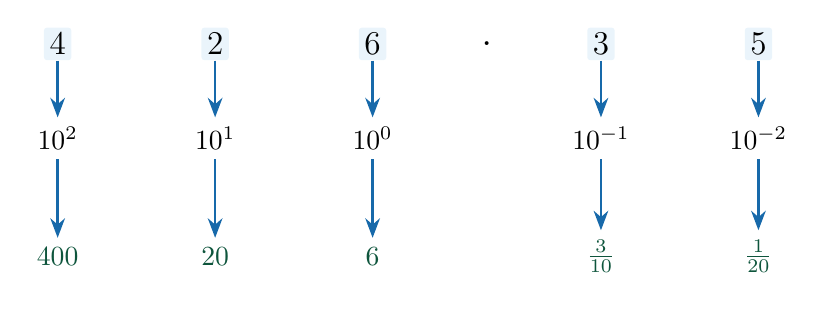
\begin{tikzpicture}[x=1mm,y=1mm]
\node[font=\large,fill=ICTLightBlue,rounded corners=1pt,inner sep=2pt] (d0) at (0,0) {$\mathrm{4}$};
\node (w0) at (0,-12) {$ 10^{2} $};
\node[text=ICTGreen!65!black] (v0) at (0,-27) {$ 400 $};
\draw[-{Stealth},draw=ICTBlue,line width=.9pt] (d0.south)--(w0.north);
\draw[-{Stealth},draw=ICTBlue,line width=.9pt] (w0.south)--(v0.north);
\node[font=\large,fill=ICTLightBlue,rounded corners=1pt,inner sep=2pt] (d1) at (20,0) {$\mathrm{2}$};
\node (w1) at (20,-12) {$ 10^{1} $};
\node[text=ICTGreen!65!black] (v1) at (20,-27) {$ 20 $};
\draw[-{Stealth},draw=ICTBlue,line width=.9pt] (d1.south)--(w1.north);
\draw[-{Stealth},draw=ICTBlue,line width=.9pt] (w1.south)--(v1.north);
\node[font=\large,fill=ICTLightBlue,rounded corners=1pt,inner sep=2pt] (d2) at (40,0) {$\mathrm{6}$};
\node (w2) at (40,-12) {$ 10^{0} $};
\node[text=ICTGreen!65!black] (v2) at (40,-27) {$ 6 $};
\draw[-{Stealth},draw=ICTBlue,line width=.9pt] (d2.south)--(w2.north);
\draw[-{Stealth},draw=ICTBlue,line width=.9pt] (w2.south)--(v2.north);
\node[font=\large,fill=ICTLightBlue,rounded corners=1pt,inner sep=2pt] (d3) at (69,0) {$\mathrm{3}$};
\node (w3) at (69,-12) {$ 10^{-1} $};
\node[text=ICTGreen!65!black] (v3) at (69,-27) {$ \frac{3}{10} $};
\draw[-{Stealth},draw=ICTBlue,line width=.9pt] (d3.south)--(w3.north);
\draw[-{Stealth},draw=ICTBlue,line width=.9pt] (w3.south)--(v3.north);
\node[font=\large,fill=ICTLightBlue,rounded corners=1pt,inner sep=2pt] (d4) at (89,0) {$\mathrm{5}$};
\node (w4) at (89,-12) {$ 10^{-2} $};
\node[text=ICTGreen!65!black] (v4) at (89,-27) {$ \frac{1}{20} $};
\draw[-{Stealth},draw=ICTBlue,line width=.9pt] (d4.south)--(w4.north);
\draw[-{Stealth},draw=ICTBlue,line width=.9pt] (w4.south)--(v4.north);
\node[font=\Large] at (54.5,0) {$.$};
\end{tikzpicture}\end{chThreeDiagram}\end{center}
\[(426.35)_{10}=4\times10^{2}+2\times10^{1}+6\times10^{0}+3\times10^{-1}+5\times10^{-2}=426.35.\]

৪-এর নিজস্ব মান ৪, কিন্তু অবদান ৪০০। পূর্ণাংশের শুরুর শূন্য বা ভগ্নাংশের শেষের শূন্য বাদ দিলে সংখ্যামান বদলায় না: $0426.350=426.35$। মাঝের বা ভগ্নাংশের শুরুর শূন্য বাদ দেওয়ার এই অনুমতি নেই।

\subsection{বাইনারি সংখ্যা পদ্ধতি}
ভিত্তি ২-এর পদ্ধতিতে শুধু 0 ও 1 অঙ্ক ব্যবহৃত হয়। একটি বাইনারি অঙ্ক হলো বিট। এর ওজন পূর্ণাংশে ১, ২, ৪, ৮, ১৬,\ldots; ভগ্নাংশে $1/2,1/4,1/8,\ldots$। গণনার শুরু: $0,1,10,11,100,101,110,111,1000$।
\smallhead{উদাহরণ: বাইনারি সংখ্যার মান}

\begin{center}\begin{chThreeDiagram}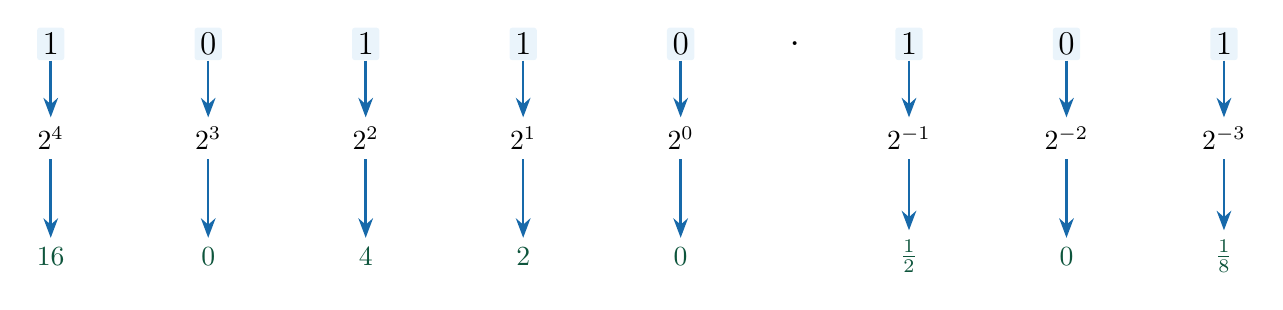
\begin{tikzpicture}[x=1mm,y=1mm]
\node[font=\large,fill=ICTLightBlue,rounded corners=1pt,inner sep=2pt] (d0) at (0,0) {$\mathrm{1}$};
\node (w0) at (0,-12) {$ 2^{4} $};
\node[text=ICTGreen!65!black] (v0) at (0,-27) {$ 16 $};
\draw[-{Stealth},draw=ICTBlue,line width=.9pt] (d0.south)--(w0.north);
\draw[-{Stealth},draw=ICTBlue,line width=.9pt] (w0.south)--(v0.north);
\node[font=\large,fill=ICTLightBlue,rounded corners=1pt,inner sep=2pt] (d1) at (20,0) {$\mathrm{0}$};
\node (w1) at (20,-12) {$ 2^{3} $};
\node[text=ICTGreen!65!black] (v1) at (20,-27) {$ 0 $};
\draw[-{Stealth},draw=ICTBlue,line width=.9pt] (d1.south)--(w1.north);
\draw[-{Stealth},draw=ICTBlue,line width=.9pt] (w1.south)--(v1.north);
\node[font=\large,fill=ICTLightBlue,rounded corners=1pt,inner sep=2pt] (d2) at (40,0) {$\mathrm{1}$};
\node (w2) at (40,-12) {$ 2^{2} $};
\node[text=ICTGreen!65!black] (v2) at (40,-27) {$ 4 $};
\draw[-{Stealth},draw=ICTBlue,line width=.9pt] (d2.south)--(w2.north);
\draw[-{Stealth},draw=ICTBlue,line width=.9pt] (w2.south)--(v2.north);
\node[font=\large,fill=ICTLightBlue,rounded corners=1pt,inner sep=2pt] (d3) at (60,0) {$\mathrm{1}$};
\node (w3) at (60,-12) {$ 2^{1} $};
\node[text=ICTGreen!65!black] (v3) at (60,-27) {$ 2 $};
\draw[-{Stealth},draw=ICTBlue,line width=.9pt] (d3.south)--(w3.north);
\draw[-{Stealth},draw=ICTBlue,line width=.9pt] (w3.south)--(v3.north);
\node[font=\large,fill=ICTLightBlue,rounded corners=1pt,inner sep=2pt] (d4) at (80,0) {$\mathrm{0}$};
\node (w4) at (80,-12) {$ 2^{0} $};
\node[text=ICTGreen!65!black] (v4) at (80,-27) {$ 0 $};
\draw[-{Stealth},draw=ICTBlue,line width=.9pt] (d4.south)--(w4.north);
\draw[-{Stealth},draw=ICTBlue,line width=.9pt] (w4.south)--(v4.north);
\node[font=\large,fill=ICTLightBlue,rounded corners=1pt,inner sep=2pt] (d5) at (109,0) {$\mathrm{1}$};
\node (w5) at (109,-12) {$ 2^{-1} $};
\node[text=ICTGreen!65!black] (v5) at (109,-27) {$ \frac{1}{2} $};
\draw[-{Stealth},draw=ICTBlue,line width=.9pt] (d5.south)--(w5.north);
\draw[-{Stealth},draw=ICTBlue,line width=.9pt] (w5.south)--(v5.north);
\node[font=\large,fill=ICTLightBlue,rounded corners=1pt,inner sep=2pt] (d6) at (129,0) {$\mathrm{0}$};
\node (w6) at (129,-12) {$ 2^{-2} $};
\node[text=ICTGreen!65!black] (v6) at (129,-27) {$ 0 $};
\draw[-{Stealth},draw=ICTBlue,line width=.9pt] (d6.south)--(w6.north);
\draw[-{Stealth},draw=ICTBlue,line width=.9pt] (w6.south)--(v6.north);
\node[font=\large,fill=ICTLightBlue,rounded corners=1pt,inner sep=2pt] (d7) at (149,0) {$\mathrm{1}$};
\node (w7) at (149,-12) {$ 2^{-3} $};
\node[text=ICTGreen!65!black] (v7) at (149,-27) {$ \frac{1}{8} $};
\draw[-{Stealth},draw=ICTBlue,line width=.9pt] (d7.south)--(w7.north);
\draw[-{Stealth},draw=ICTBlue,line width=.9pt] (w7.south)--(v7.north);
\node[font=\Large] at (94.5,0) {$.$};
\end{tikzpicture}\end{chThreeDiagram}\end{center}
\[(10110.101)_{2}=1\times2^{4}+0\times2^{3}+1\times2^{2}+1\times2^{1}+0\times2^{0}+1\times2^{-1}+0\times2^{-2}+1\times2^{-3}=22.625.\]

\smallhead{কম্পিউটারে বাইনারি সুবিধাজনক কেন?}
ডিজিটাল সার্কিটে দুটি পৃথক ভোল্টেজ-পরিসর দিয়ে ০ ও ১ বোঝানো সুবিধাজনক। সামান্য বৈদ্যুতিক পরিবর্তন হলেও নির্ধারিত সীমার মধ্যে থাকলে একই logical state পাওয়া যায়। এই দুটি অবস্থা দিয়ে স্মৃতিতে তথ্য রাখা এবং লজিক গেটের সাহায্যে গণনা করা যায়। বিট ০ মানেই সর্বত্র একেবারে বিদ্যুৎ নেই—এমন অর্থ নয়; ০ ও ১ হলো নির্ধারিত অবস্থার প্রতীক। দীর্ঘ বাইনারি লেখা পড়ার সুবিধায় অক্টাল ও হেক্সাডেসিমাল ব্যবহার করা হয়।

\subsection{অক্টাল সংখ্যা পদ্ধতি}
ভিত্তি ৮-এর পদ্ধতিতে 0–7 অঙ্ক ব্যবহৃত হয়। ৭-এর পরের পূর্ণসংখ্যা $(10)_8$; এখানে ৮ বা ৯ অঙ্ক নেই। $8=2^3$ হওয়ায় প্রতিটি অক্টাল অঙ্ককে ঠিক ৩ বিটে প্রকাশ করা যায়। ফলে বাইনারির দীর্ঘ লেখা সংক্ষিপ্ত হয়। কিছু কম্পিউটার ব্যবস্থায় অনুমতি বা mode প্রকাশেও অক্টাল দেখা যায়।
\smallhead{উদাহরণ: অক্টালের পূর্ণ ও ভগ্নাংশ}

\begin{center}\begin{chThreeDiagram}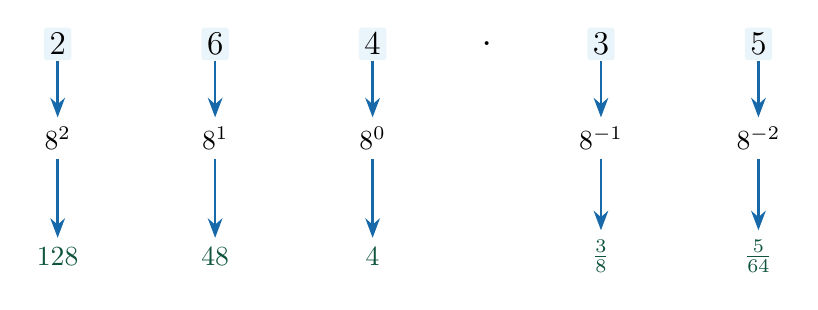
\begin{tikzpicture}[x=1mm,y=1mm]
\node[font=\large,fill=ICTLightBlue,rounded corners=1pt,inner sep=2pt] (d0) at (0,0) {$\mathrm{2}$};
\node (w0) at (0,-12) {$ 8^{2} $};
\node[text=ICTGreen!65!black] (v0) at (0,-27) {$ 128 $};
\draw[-{Stealth},draw=ICTBlue,line width=.9pt] (d0.south)--(w0.north);
\draw[-{Stealth},draw=ICTBlue,line width=.9pt] (w0.south)--(v0.north);
\node[font=\large,fill=ICTLightBlue,rounded corners=1pt,inner sep=2pt] (d1) at (20,0) {$\mathrm{6}$};
\node (w1) at (20,-12) {$ 8^{1} $};
\node[text=ICTGreen!65!black] (v1) at (20,-27) {$ 48 $};
\draw[-{Stealth},draw=ICTBlue,line width=.9pt] (d1.south)--(w1.north);
\draw[-{Stealth},draw=ICTBlue,line width=.9pt] (w1.south)--(v1.north);
\node[font=\large,fill=ICTLightBlue,rounded corners=1pt,inner sep=2pt] (d2) at (40,0) {$\mathrm{4}$};
\node (w2) at (40,-12) {$ 8^{0} $};
\node[text=ICTGreen!65!black] (v2) at (40,-27) {$ 4 $};
\draw[-{Stealth},draw=ICTBlue,line width=.9pt] (d2.south)--(w2.north);
\draw[-{Stealth},draw=ICTBlue,line width=.9pt] (w2.south)--(v2.north);
\node[font=\large,fill=ICTLightBlue,rounded corners=1pt,inner sep=2pt] (d3) at (69,0) {$\mathrm{3}$};
\node (w3) at (69,-12) {$ 8^{-1} $};
\node[text=ICTGreen!65!black] (v3) at (69,-27) {$ \frac{3}{8} $};
\draw[-{Stealth},draw=ICTBlue,line width=.9pt] (d3.south)--(w3.north);
\draw[-{Stealth},draw=ICTBlue,line width=.9pt] (w3.south)--(v3.north);
\node[font=\large,fill=ICTLightBlue,rounded corners=1pt,inner sep=2pt] (d4) at (89,0) {$\mathrm{5}$};
\node (w4) at (89,-12) {$ 8^{-2} $};
\node[text=ICTGreen!65!black] (v4) at (89,-27) {$ \frac{5}{64} $};
\draw[-{Stealth},draw=ICTBlue,line width=.9pt] (d4.south)--(w4.north);
\draw[-{Stealth},draw=ICTBlue,line width=.9pt] (w4.south)--(v4.north);
\node[font=\Large] at (54.5,0) {$.$};
\end{tikzpicture}\end{chThreeDiagram}\end{center}
\[(264.35)_{8}=2\times8^{2}+6\times8^{1}+4\times8^{0}+3\times8^{-1}+5\times8^{-2}=180.453125.\]

বিন্দুর ডানের প্রথম ওজন $1/8$, দ্বিতীয়টি $1/64$। তাই $(0.1)_8$-কে দশমিক ০.১ ধরা যাবে না; এর দশমিক মান ০.১২৫।

\subsection{হেক্সাডেসিমাল সংখ্যা পদ্ধতি}
ভিত্তি ১৬-এর পদ্ধতিতে 0–9 এবং A–F মোট ১৬টি অঙ্ক ব্যবহৃত হয়। এখানে A=10, B=11, C=12, D=13, E=14, F=15। F-এর পরের সংখ্যা $(10)_{16}$। $16=2^4$ হওয়ায় প্রতি অঙ্কে ৪ বিট লাগে। এক বাইটের মান দুইটি হেক্সাডেসিমাল অঙ্কে লেখা যায়।
\Needspace{10\baselineskip}
\smallhead{উদাহরণ: অক্ষর-প্রতীকের সংখ্যামান}

\begin{center}\begin{chThreeDiagram}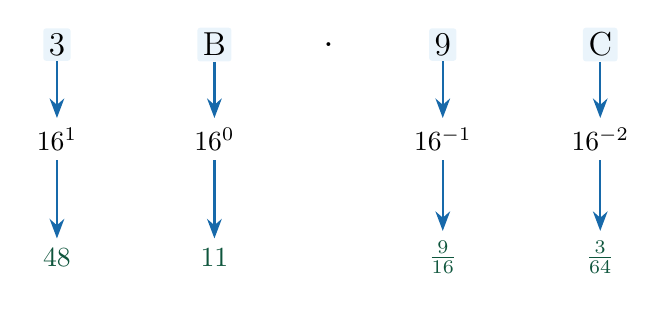
\begin{tikzpicture}[x=1mm,y=1mm]
\node[font=\large,fill=ICTLightBlue,rounded corners=1pt,inner sep=2pt] (d0) at (0,0) {$\mathrm{3}$};
\node (w0) at (0,-12) {$ 16^{1} $};
\node[text=ICTGreen!65!black] (v0) at (0,-27) {$ 48 $};
\draw[-{Stealth},draw=ICTBlue,line width=.9pt] (d0.south)--(w0.north);
\draw[-{Stealth},draw=ICTBlue,line width=.9pt] (w0.south)--(v0.north);
\node[font=\large,fill=ICTLightBlue,rounded corners=1pt,inner sep=2pt] (d1) at (20,0) {$\mathrm{B}$};
\node (w1) at (20,-12) {$ 16^{0} $};
\node[text=ICTGreen!65!black] (v1) at (20,-27) {$ 11 $};
\draw[-{Stealth},draw=ICTBlue,line width=.9pt] (d1.south)--(w1.north);
\draw[-{Stealth},draw=ICTBlue,line width=.9pt] (w1.south)--(v1.north);
\node[font=\large,fill=ICTLightBlue,rounded corners=1pt,inner sep=2pt] (d2) at (49,0) {$\mathrm{9}$};
\node (w2) at (49,-12) {$ 16^{-1} $};
\node[text=ICTGreen!65!black] (v2) at (49,-27) {$ \frac{9}{16} $};
\draw[-{Stealth},draw=ICTBlue,line width=.9pt] (d2.south)--(w2.north);
\draw[-{Stealth},draw=ICTBlue,line width=.9pt] (w2.south)--(v2.north);
\node[font=\large,fill=ICTLightBlue,rounded corners=1pt,inner sep=2pt] (d3) at (69,0) {$\mathrm{C}$};
\node (w3) at (69,-12) {$ 16^{-2} $};
\node[text=ICTGreen!65!black] (v3) at (69,-27) {$ \frac{3}{64} $};
\draw[-{Stealth},draw=ICTBlue,line width=.9pt] (d3.south)--(w3.north);
\draw[-{Stealth},draw=ICTBlue,line width=.9pt] (w3.south)--(v3.north);
\node[font=\Large] at (34.5,0) {$.$};
\end{tikzpicture}\end{chThreeDiagram}\end{center}
\[(3B.9C)_{16}=3\times16^{1}+11\times16^{0}+9\times16^{-1}+12\times16^{-2}=59.609375.\]

এখানে B ও C-এর মান যথাক্রমে ১১ ও ১২। মেমোরি ঠিকানা, মেশিন নির্দেশের byte এবং রঙের মান সংক্ষেপে দেখাতে হেক্সাডেসিমাল সুবিধাজনক। যেমন RGB রঙের তিনটি byte প্রায়ই ছয়টি হেক্সাডেসিমাল অঙ্কে লেখা হয়।

\subsection{চার পদ্ধতির তুলনা ও ধারাবাহিক গণনা}
নিচের প্রতিটি সারি একই পরিমাণের চারটি প্রকাশ। বাইনারির শুরুতে প্রয়োজনমতো শূন্য বসিয়ে চার বিট রাখা হয়েছে, যাতে হেক্সাডেসিমাল অঙ্কের সঙ্গে মিল বোঝা যায়।
\begin{center}\begin{tabular}{|c|c|c|c|}\hline
\rowcolor{ICTLightBlue}দশমিক&বাইনারি&অক্টাল&হেক্সাডেসিমাল\\\hline
0&0000&0&0\\\hline
1&0001&1&1\\\hline
2&0010&2&2\\\hline
3&0011&3&3\\\hline
4&0100&4&4\\\hline
5&0101&5&5\\\hline
6&0110&6&6\\\hline
7&0111&7&7\\\hline
8&1000&10&8\\\hline
9&1001&11&9\\\hline
10&1010&12&A\\\hline
11&1011&13&B\\\hline
12&1100&14&C\\\hline
13&1101&15&D\\\hline
14&1110&16&E\\\hline
15&1111&17&F\\\hline
16&10000&20&10\\\hline
31&11111&37&1F\\\hline
32&100000&40&20\\\hline
63&111111&77&3F\\\hline
64&1000000&100&40\\\hline
\end{tabular}\end{center}
\textbf{একই ১০-এর অর্থ:} যেকোনো ভিত্তি $b$-তে $(10)_b=b$। তাই $(10)_2=2$, $(10)_8=8$ এবং $(10)_{16}=16$ দশমিক মান প্রকাশ করে। শুধু লেখার দৈর্ঘ্য দেখে ভিন্ন ভিত্তির দুটি সংখ্যা তুলনা করা যায় না।

\smallhead{উদাহরণ: আগের ও পরের পূর্ণসংখ্যা}
\begin{center}\begin{tabular}{|c|c|c|}\hline
আগের সংখ্যা&প্রদত্ত সংখ্যা&পরের সংখ্যা\\\hline
$(76)_8$&$(77)_8$&$(100)_8$\\\hline
$(2E)_{16}$&$(2F)_{16}$&$(30)_{16}$\\\hline
$(1110)_2$&$(1111)_2$&$(10000)_2$\\\hline
\end{tabular}\end{center}
সর্বোচ্চ অঙ্কে ১ যোগ হলে ০ রেখে বাম ঘরে ক্যারি যায়। ঠিক আগের সংখ্যা পেতে প্রয়োজন হলে বাম ঘর থেকে ধার নিতে হয়। চার বিটের সীমা বেঁধে দিলে 1111-এর পর অতিরিক্ত ক্যারি বাদ দিয়ে 0000 থাকে; সীমাহীন পূর্ণসংখ্যা গণনায় পরের মান 10000।

\subsection{বিট, নিবল, বাইট ও ওয়ার্ড}
\begin{center}\begin{tabularx}{\linewidth}{|L{.18\linewidth}|L{.22\linewidth}|Y|}\hline
\rowcolor{ICTLightBlue}একক&সম্পর্ক&ব্যাখ্যা\\\hline
বিট&একটি 0 বা 1&দুইটি পৃথক অবস্থা প্রকাশ করে\\\hline
নিবল&4 বিট&একটি হেক্সাডেসিমাল অঙ্কের সমান দৈর্ঘ্য\\\hline
বাইট&8 বিট&দুই নিবল; ২৫৬টি পৃথক bit pattern\\\hline
ওয়ার্ড&স্থাপত্যনির্ভর দৈর্ঘ্য&প্রসেসরের স্বাভাবিক তথ্যপ্রক্রিয়াকরণ একক; সব ক্ষেত্রে এক বাইট নয়\\\hline
\end{tabularx}\end{center}
৩২-বিট ওয়ার্ডে ৪ বাইট, ৬৪-বিট ওয়ার্ডে ৮ বাইট। একটি ক্যারেক্টার সবসময় এক বাইটে থাকে না; কোন encoding ব্যবহৃত হয়েছে তার ওপর দৈর্ঘ্য নির্ভর করে। বড় এককে decimal prefix ও binary prefix আলাদা: $1\,\mathrm{kB}=1000\,\mathrm{B}$, $1\,\mathrm{KiB}=1024\,\mathrm{B}$। একইভাবে $1\,\mathrm{MiB}=2^{20}\,\mathrm{B}$।

\smallhead{অবস্থার সংখ্যা, পরিসর ও প্রয়োজনীয় বিট}
$n$ বিটে $2^n$টি পৃথক pattern পাওয়া যায়। চিহ্নবিহীন পূর্ণসংখ্যা হিসেবে মানের পরিসর $0$ থেকে $2^n-1$। $N$টি আলাদা বস্তু শনাক্ত করতে ক্ষুদ্রতম এমন $n$ নিতে হবে যেন $2^n\ge N$।

\textbf{উদাহরণ ১:} ৫ বিটে ৩২টি অবস্থা; সর্বোচ্চ unsigned মান $31=(11111)_2$। ৩২টি অবস্থা মানে সর্বোচ্চ মান ৩২ নয়, কারণ শূন্যও একটি অবস্থা।\\
\textbf{উদাহরণ ২:} ৭০টি যন্ত্রের আলাদা পরিচয় দিতে ৭ বিট প্রয়োজন: $2^6=64<70\le128=2^7$। ৮০টি পরিচয় হলে একই ৭ বিট যথেষ্ট।\\
\textbf{উদাহরণ ৩:} অক্টালের একটি অঙ্কের জন্য ৩ বিট এবং হেক্সাডেসিমালের জন্য ৪ বিট লাগে। পুরো সংখ্যার দৈর্ঘ্য অঙ্কসংখ্যা ও leading zero রাখার শর্তের ওপর নির্ভর করে।

\subsection{ধারণা থেকে সমাধান}
\smallhead{অজানা ভিত্তি নির্ণয়}
$(12)_b+(15)_b=(30)_b$ হলে $(b+2)+(b+5)=3b$। তাই $b=7$। বৃহত্তম অঙ্ক ৫ ভিত্তির চেয়ে ছোট হওয়ায় ফল গ্রহণযোগ্য। দশমিক যাচাই: $9+12=21$। কেবল সমীকরণ মিললেই হবে না; প্রতিটি অঙ্কও বৈধ হতে হবে।

\smallhead{জ্ঞান ও অনুধাবন}
\textbf{ক. র‍্যাডিক্স পয়েন্ট কী?} স্থানিক সংখ্যার পূর্ণাংশ ও ভগ্নাংশের বিভাজক।\\
\textbf{খ. একই অঙ্কের মান অবস্থানভেদে বদলায় কেন?} অঙ্কের অবদান হয় নিজস্ব মান ও অবস্থানের ওজনের গুণফল; অবস্থান বদলালে ওজন বদলায়।\\
\textbf{খ. হেক্সাডেসিমাল কম্পিউটারের তথ্য দেখাতে সুবিধাজনক কেন?} চারটি বাইনারি বিটকে একটি অঙ্কে দেখানো যায়, ফলে দীর্ঘ bit pattern সংক্ষিপ্ত ও সহজপাঠ্য হয়।

\smallhead{ধারণাভিত্তিক MCQ}
$(65)_b$ বৈধ হলে $b$-এর সর্বনিম্ন মান কত? (ক) ৫, (খ) ৬, (গ) ৭, (ঘ) ৮।\\
\textbf{সমাধান:} (গ) ৭। বৃহত্তম অঙ্ক ৬; ভিত্তি তার চেয়ে বড় হতে হবে। এটি সর্বনিম্ন গ্রহণযোগ্য ভিত্তি, একমাত্র সম্ভাব্য ভিত্তি নয়।

% VISUAL_CONVERSION_V2: generated lessons; original snapshot is in build/chapter03_update/visual_conversion/baseline.
\Needspace{9\baselineskip}
\section{সংখ্যা পদ্ধতির রূপান্তর (\textenglish{Conversion of Number Systems})}
% Reusable styles shared by all generated visual conversion lessons.
\usetikzlibrary{arrows.meta,calc,decorations.pathreplacing}
\definecolor{vcBlue}{HTML}{166A9E}
\definecolor{vcGreen}{HTML}{087563}
\definecolor{vcPad}{HTML}{945000}
\tikzset{vcnum/.style={font=\normalsize,inner sep=.5pt,minimum height=4mm},
vc digit/.style={font=\large,inner sep=1.3pt,minimum height=4mm,text=vcBlue!80!black,fill=vcBlue!7,rounded corners=1pt},
vc result/.style={vc digit,text=vcGreen!80!black,fill=vcGreen!8},
vc bit/.style={font=\normalsize,inner sep=.5pt,minimum height=4mm},
vcnote/.style={font=\small,inner sep=.5pt,align=center},
vc arrow/.style={-{Stealth[length=1.9mm,width=1.3mm]},draw=vcBlue,line width=.9pt,shorten <=.7pt,shorten >=.7pt},
vc line/.style={draw=vcBlue!75!black,line width=.8pt},
vc brace/.style={decorate,decoration={brace,mirror,amplitude=1.2mm},draw=vcBlue,line width=.85pt}}
\newcommand{\convExample}[2]{\par\vspace{2mm}\noindent\textcolor{ICTGreen!65!black}{\textbf{উদাহরণ #1: #2}}\par\vspace{1mm}}

\subsection{রূপান্তরের নিয়ম ও পথ নির্বাচন}
রূপান্তরে সংখ্যার মান অপরিবর্তিত থাকে; অঙ্ক ও ভিত্তি বদলায়। যেমন $(13)_{10}=(1101)_2$। বিন্দুর আগে পূর্ণাংশ এবং পরে ভগ্নাংশ; দুই অংশের নিয়ম আলাদা।
\begin{center}\begin{tabularx}{\linewidth}{|L{.26\linewidth}|Y|L{.23\linewidth}|}\hline
রূপান্তর & করণীয় & পড়ার ক্রম\\\hline
Decimal পূর্ণাংশ & লক্ষ্য ভিত্তি দিয়ে ভাগ; নতুন ভাগফল নিয়ে আবার ভাগ & ভাগশেষ নিচ থেকে ওপরে\\\hline
Decimal ভগ্নাংশ & লক্ষ্য ভিত্তি দিয়ে গুণ; নতুন ভগ্নাংশ নিয়ে আবার গুণ & প্রাপ্ত অঙ্ক ওপর থেকে নিচে\\\hline
Base-$b$ থেকে Decimal & অঙ্ক $\times b^{\text{অবস্থান}}$; সব অবদান যোগ & বিন্দুতে $b^0$ ও $b^{-1}$\\\hline
Binary ও Octal & ৩ বিটে একটি অক্টাল অঙ্ক & বিন্দু থেকে দুই দিকে\\\hline
Binary ও Hexadecimal & ৪ বিটে একটি হেক্সাডেসিমাল অঙ্ক & বিন্দু থেকে দুই দিকে\\\hline
Octal ও Hexadecimal & প্রতিটি অঙ্কের binary; তারপর নতুন grouping & অঙ্ক ও বিটের ক্রম একই\\\hline
Base-$m$ থেকে Base-$n$ & প্রথমে Decimal, তারপর লক্ষ্য ভিত্তি & পূর্ণাংশ ও ভগ্নাংশ পৃথক\\\hline
\end{tabularx}\end{center}
\smallhead{সংক্ষিপ্ত কাজের ধাপ}
\begin{compactenum}
\item source ও target base এবং বৈধ digit যাচাই করো।
\item পূর্ণাংশ ও ভগ্নাংশ আলাদা করো; প্রযোজ্য নিয়মে সব ধাপ দেখাও।
\item প্রতিটি group বা ধাপের digit সঠিক ক্রমে বসিয়ে base লিখো।
\item স্থানমান বা বিপরীত রূপান্তরে মান যাচাই করো।
\end{compactenum}
\smallhead{হেক্সাডেসিমাল অঙ্কের প্রয়োজনীয় মান}
\begin{center}\begin{tabular}{|c|c|c|c|c|c|c|}\hline
দশমিক&10&11&12&13&14&15\\\hline
অঙ্ক&A&B&C&D&E&F\\\hline
\end{tabular}\end{center}
প্রথম প্রাপ্ত ভাগশেষ পূর্ণাংশের LSB, শেষটি MSB; উত্তর লেখা হয় MSB থেকে। ভগ্নাংশে প্রথম অঙ্ক সবচেয়ে গুরুত্বপূর্ণ, তাই পাওয়া ক্রমেই লেখা হয়। নির্দিষ্ট দৈর্ঘ্যে অসীম ভগ্নাংশ থামালে ফলের আগে $\approx$ দিতে হবে।
\smallhead{পূর্ণাংশে ভাগ কেন, ভগ্নাংশে গুণ কেন?}
পূর্ণসংখ্যা $N$-কে ভিত্তি $b$ দিয়ে ভাগ করলে $N=bq+r$, যেখানে $0\le r<b$। তাই $r$ এককের অঙ্ক, আর $q$-তে বাকি অঙ্কগুলো থাকে। ভাগ চালিয়ে শেষ ভাগশেষ থেকে পড়লে উচ্চ ওজনের অঙ্ক আগে পাওয়া যায়। ভগ্নাংশ $f$-এর জন্য $bf=d+f'$; এখানে পূর্ণাংশ $d$ প্রথম ভগ্নাংশ অঙ্ক এবং অবশিষ্ট $f'$ নিয়ে পরের ধাপ হয়। এজন্য গুণে পাওয়া অঙ্ক প্রথম থেকে পড়তে হয়।

\smallhead{গ্রুপিং কোথা থেকে শুরু হবে?}
পূর্ণাংশে বিন্দু থেকে বামে এবং ভগ্নাংশে বিন্দু থেকে ডানে গ্রুপ করো। $8=2^3$ বলে অক্টালে ৩ বিট, $16=2^4$ বলে হেক্সাডেসিমালে ৪ বিট এক অঙ্ক। অসম্পূর্ণ গ্রুপ পূরণে পূর্ণাংশের একেবারে বামে বা ভগ্নাংশের একেবারে ডানে ০ বসে। এই ০ নতুন পরিমাণ যোগ করে না; মাঝখানে বা ভগ্নাংশের শুরুতে বসালে মান বদলাবে।

\textbf{চিত্রের সংকেত:} নীল arrow ধাপের সংযোগ, নীল brace বিটের দল, সবুজ অঙ্ক রূপান্তরের ফল এবং বাদামি টীকা প্রয়োজনীয় zero padding নির্দেশ করে। দাগঘেরা সীমানা থাকায় সাদা-কালো ছাপাতেও padding চেনা যায়।

\smallhead{দশমিক ও বাইনারির পারস্পরিক রূপান্তর}
\subsection{দশমিক থেকে বাইনারি}
পূর্ণাংশে লক্ষ্য ভিত্তি দিয়ে ভাগ করো; ভাগশেষ নিচ থেকে ওপরে পড়ো। ভগ্নাংশে একই ভিত্তি দিয়ে গুণ করে পাওয়া অঙ্ক ওপর থেকে নিচে পড়ো।
\par\noindent\begin{minipage}{\linewidth}
\convExample{১}{পূর্ণসংখ্যা}
$ (45)_{10} $-কে ২ ভিত্তিতে রূপান্তর করো।\par
\par\noindent\begin{minipage}{\linewidth}\centering
\phantomsection\label{VC001}
\begin{chThreeDiagram}\begin{tikzpicture}[x=1mm,y=1mm]
\path[use as bounding box] (-3,9) rectangle (72,-56);
\node[vcnote] at (15,7) {ভাজ্য/ভাগফল};
\node[vcnote] at (44,7) {ভাগশেষ};
\node[vcnum] at (0.0,0) {$ 2 $};
\node[vcnum] at (10.0,0) {$ 45 $};
\draw[vc line] (5.0,3)--(5.0,-3.5)--(50,-3.5);
\node[vcnum] (r0) at (44,-7) {$ 1 $};
\node[vcnum] at (1.5,-7) {$ 2 $};
\node[vcnum] at (11.5,-7) {$ 22 $};
\draw[vc line] (6.5,-4)--(6.5,-10.5)--(50,-10.5);
\node[vcnum] (r1) at (44,-14) {$ 0 $};
\node[vcnum] at (3.0,-14) {$ 2 $};
\node[vcnum] at (13.0,-14) {$ 11 $};
\draw[vc line] (8.0,-11)--(8.0,-17.5)--(50,-17.5);
\node[vcnum] (r2) at (44,-21) {$ 1 $};
\node[vcnum] at (4.5,-21) {$ 2 $};
\node[vcnum] at (14.5,-21) {$ 5 $};
\draw[vc line] (9.5,-18)--(9.5,-24.5)--(50,-24.5);
\node[vcnum] (r3) at (44,-28) {$ 1 $};
\node[vcnum] at (6.0,-28) {$ 2 $};
\node[vcnum] at (16.0,-28) {$ 2 $};
\draw[vc line] (11.0,-25)--(11.0,-31.5)--(50,-31.5);
\node[vcnum] (r4) at (44,-35) {$ 0 $};
\node[vcnum] at (7.5,-35) {$ 2 $};
\node[vcnum] at (17.5,-35) {$ 1 $};
\draw[vc line] (12.5,-32)--(12.5,-38.5)--(50,-38.5);
\node[vcnum] (r5) at (44,-42) {$ 1 $};
\node[vcnum] at (19.0,-42) {$0$};
\node[vcnote] at (61,-3) {LSB};
\node[vcnote] at (61,-47) {MSB};
\draw[vc arrow] (61,-42)--(61,-7);
\node[vcnote] at (31,-54) {নিচ থেকে ওপরে পড়ো};
\end{tikzpicture}\end{chThreeDiagram}
\end{minipage}\par
\[\therefore\ (45)_{10}=(101101)_{2}.\]
\end{minipage}\par
\par\noindent\begin{minipage}{\linewidth}
\convExample{২}{শুধু ভগ্নাংশ}
$ (0.6875)_{10} $-কে ২ ভিত্তিতে রূপান্তর করো।\par
\par\noindent\begin{minipage}{\linewidth}\centering
\phantomsection\label{VC002}
\begin{chThreeDiagram}\begin{tikzpicture}[x=1mm,y=1mm]
\path[use as bounding box] (-9,9) rectangle (76,-63);
\node[vcnote] at (14,7) {প্রাপ্ত অঙ্ক};
\node[vcnote] at (45,7) {ভগ্নাংশ};
\node[vcnum] at (45,0) {$ 0.6875 $};
\draw[vc line] (26,3)--(26,-51);
\node[vcnum] (m0) at (45,-5) {$\times 2$};
\draw[vc line] (7,-8)--(65,-8);
\node[vcnum] at (14,-12) {$ 1 $};
\node[vcnum] (f0) at (45,-12) {$ 0.375 $};
\node[vcnum] (m1) at (45,-17) {$\times 2$};
\draw[vc line] (7,-20)--(65,-20);
\node[vcnum] at (14,-24) {$ 0 $};
\node[vcnum] (f1) at (45,-24) {$ 0.75 $};
\node[vcnum] (m2) at (45,-29) {$\times 2$};
\draw[vc line] (7,-32)--(65,-32);
\node[vcnum] at (14,-36) {$ 1 $};
\node[vcnum] (f2) at (45,-36) {$ 0.5 $};
\node[vcnum] (m3) at (45,-41) {$\times 2$};
\draw[vc line] (7,-44)--(65,-44);
\node[vcnum] at (14,-48) {$ 1 $};
\node[vcnum] (f3) at (45,-48) {$ 0 $};
\draw[vc arrow] (f0.east)--(72,-12)--(72,-17)--(m1.east);
\draw[vc arrow] (f1.east)--(72,-24)--(72,-29)--(m2.east);
\draw[vc arrow] (f2.east)--(72,-36)--(72,-41)--(m3.east);
\node[vcnote] at (0,-8) {MSB};
\node[vcnote] at (0,-53) {LSB};
\draw[vc arrow] (0,-12)--(0,-48);
\node[vcnote] at (34,-60) {ওপর থেকে নিচে পড়ো};
\end{tikzpicture}\end{chThreeDiagram}
\end{minipage}\par
\[\therefore\ (0.6875)_{10}=(0.1011)_{2}.\]
\end{minipage}\par
\par\noindent\begin{minipage}{\linewidth}
\convExample{৩}{মিশ্র সংখ্যা}
$ (77.4375)_{10} $-কে ২ ভিত্তিতে রূপান্তর করো।\par
\begin{minipage}[t]{.48\linewidth}\vspace{0pt}\centering\textbf{পূর্ণাংশ}\par\vspace{1mm}
\par\noindent\begin{minipage}{\linewidth}\centering
\phantomsection\label{VC003}
\begin{chThreeDiagram}\begin{tikzpicture}[x=1mm,y=1mm]
\path[use as bounding box] (-3,9) rectangle (72,-63);
\node[vcnote] at (15,7) {ভাজ্য/ভাগফল};
\node[vcnote] at (44,7) {ভাগশেষ};
\node[vcnum] at (0.0,0) {$ 2 $};
\node[vcnum] at (10.0,0) {$ 77 $};
\draw[vc line] (5.0,3)--(5.0,-3.5)--(50,-3.5);
\node[vcnum] (r0) at (44,-7) {$ 1 $};
\node[vcnum] at (1.5,-7) {$ 2 $};
\node[vcnum] at (11.5,-7) {$ 38 $};
\draw[vc line] (6.5,-4)--(6.5,-10.5)--(50,-10.5);
\node[vcnum] (r1) at (44,-14) {$ 0 $};
\node[vcnum] at (3.0,-14) {$ 2 $};
\node[vcnum] at (13.0,-14) {$ 19 $};
\draw[vc line] (8.0,-11)--(8.0,-17.5)--(50,-17.5);
\node[vcnum] (r2) at (44,-21) {$ 1 $};
\node[vcnum] at (4.5,-21) {$ 2 $};
\node[vcnum] at (14.5,-21) {$ 9 $};
\draw[vc line] (9.5,-18)--(9.5,-24.5)--(50,-24.5);
\node[vcnum] (r3) at (44,-28) {$ 1 $};
\node[vcnum] at (6.0,-28) {$ 2 $};
\node[vcnum] at (16.0,-28) {$ 4 $};
\draw[vc line] (11.0,-25)--(11.0,-31.5)--(50,-31.5);
\node[vcnum] (r4) at (44,-35) {$ 0 $};
\node[vcnum] at (7.5,-35) {$ 2 $};
\node[vcnum] at (17.5,-35) {$ 2 $};
\draw[vc line] (12.5,-32)--(12.5,-38.5)--(50,-38.5);
\node[vcnum] (r5) at (44,-42) {$ 0 $};
\node[vcnum] at (9.0,-42) {$ 2 $};
\node[vcnum] at (19.0,-42) {$ 1 $};
\draw[vc line] (14.0,-39)--(14.0,-45.5)--(50,-45.5);
\node[vcnum] (r6) at (44,-49) {$ 1 $};
\node[vcnum] at (20.5,-49) {$0$};
\node[vcnote] at (61,-3) {LSB};
\node[vcnote] at (61,-54) {MSB};
\draw[vc arrow] (61,-49)--(61,-7);
\node[vcnote] at (31,-61) {নিচ থেকে ওপরে পড়ো};
\end{tikzpicture}\end{chThreeDiagram}
\end{minipage}\par

$ (1001101)_{2} $
\end{minipage}\hfill
\begin{minipage}[t]{.48\linewidth}\vspace{0pt}\centering\textbf{ভগ্নাংশ}\par\vspace{1mm}
\par\noindent\begin{minipage}{\linewidth}\centering
\phantomsection\label{VC004}
\begin{chThreeDiagram}\begin{tikzpicture}[x=1mm,y=1mm]
\path[use as bounding box] (-9,9) rectangle (76,-63);
\node[vcnote] at (14,7) {প্রাপ্ত অঙ্ক};
\node[vcnote] at (45,7) {ভগ্নাংশ};
\node[vcnum] at (45,0) {$ 0.4375 $};
\draw[vc line] (26,3)--(26,-51);
\node[vcnum] (m0) at (45,-5) {$\times 2$};
\draw[vc line] (7,-8)--(65,-8);
\node[vcnum] at (14,-12) {$ 0 $};
\node[vcnum] (f0) at (45,-12) {$ 0.875 $};
\node[vcnum] (m1) at (45,-17) {$\times 2$};
\draw[vc line] (7,-20)--(65,-20);
\node[vcnum] at (14,-24) {$ 1 $};
\node[vcnum] (f1) at (45,-24) {$ 0.75 $};
\node[vcnum] (m2) at (45,-29) {$\times 2$};
\draw[vc line] (7,-32)--(65,-32);
\node[vcnum] at (14,-36) {$ 1 $};
\node[vcnum] (f2) at (45,-36) {$ 0.5 $};
\node[vcnum] (m3) at (45,-41) {$\times 2$};
\draw[vc line] (7,-44)--(65,-44);
\node[vcnum] at (14,-48) {$ 1 $};
\node[vcnum] (f3) at (45,-48) {$ 0 $};
\draw[vc arrow] (f0.east)--(72,-12)--(72,-17)--(m1.east);
\draw[vc arrow] (f1.east)--(72,-24)--(72,-29)--(m2.east);
\draw[vc arrow] (f2.east)--(72,-36)--(72,-41)--(m3.east);
\node[vcnote] at (0,-8) {MSB};
\node[vcnote] at (0,-53) {LSB};
\draw[vc arrow] (0,-12)--(0,-48);
\node[vcnote] at (34,-60) {ওপর থেকে নিচে পড়ো};
\end{tikzpicture}\end{chThreeDiagram}
\end{minipage}\par

$ (0.0111)_{2} $
\end{minipage}\par
\[\therefore\ (77.4375)_{10}=(1001101.0111)_{2}.\]
\end{minipage}\par

\subsection{বাইনারি থেকে দশমিক}
বিন্দুর বামে ওজন $b^0,b^1,\ldots$; ডানে $b^{-1},b^{-2},\ldots$। প্রতিটি অঙ্কের সঙ্গে তার ওজন গুণ করে অবদানগুলো যোগ করো।
\par\noindent\begin{minipage}{\linewidth}
\convExample{১}{পূর্ণসংখ্যা}
$ (101101)_{2} $-কে ১০ ভিত্তিতে রূপান্তর করো।\par
\par\noindent\begin{minipage}{\linewidth}\centering
\phantomsection\label{VC017}
\begin{chThreeDiagram}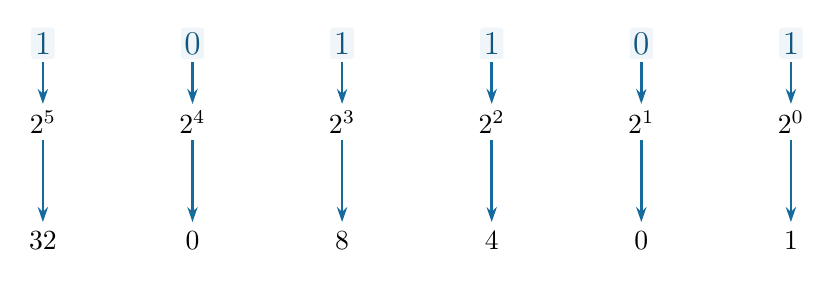
\begin{tikzpicture}[x=1mm,y=1mm]
\node[vc digit] (d0) at (0,0) {$ 1 $};
\node[vcnum] (w0) at (0,-10) {$ 2^{5} $};
\node[vcnum] (v0) at (0,-25) {$ 32 $};
\draw[vc arrow] (d0.south)--(w0.north);
\draw[vc arrow] (w0.south)--(v0.north);
\node[vc digit] (d1) at (19,0) {$ 0 $};
\node[vcnum] (w1) at (19,-10) {$ 2^{4} $};
\node[vcnum] (v1) at (19,-25) {$ 0 $};
\draw[vc arrow] (d1.south)--(w1.north);
\draw[vc arrow] (w1.south)--(v1.north);
\node[vc digit] (d2) at (38,0) {$ 1 $};
\node[vcnum] (w2) at (38,-10) {$ 2^{3} $};
\node[vcnum] (v2) at (38,-25) {$ 8 $};
\draw[vc arrow] (d2.south)--(w2.north);
\draw[vc arrow] (w2.south)--(v2.north);
\node[vc digit] (d3) at (57,0) {$ 1 $};
\node[vcnum] (w3) at (57,-10) {$ 2^{2} $};
\node[vcnum] (v3) at (57,-25) {$ 4 $};
\draw[vc arrow] (d3.south)--(w3.north);
\draw[vc arrow] (w3.south)--(v3.north);
\node[vc digit] (d4) at (76,0) {$ 0 $};
\node[vcnum] (w4) at (76,-10) {$ 2^{1} $};
\node[vcnum] (v4) at (76,-25) {$ 0 $};
\draw[vc arrow] (d4.south)--(w4.north);
\draw[vc arrow] (w4.south)--(v4.north);
\node[vc digit] (d5) at (95,0) {$ 1 $};
\node[vcnum] (w5) at (95,-10) {$ 2^{0} $};
\node[vcnum] (v5) at (95,-25) {$ 1 $};
\draw[vc arrow] (d5.south)--(w5.north);
\draw[vc arrow] (w5.south)--(v5.north);
\end{tikzpicture}\end{chThreeDiagram}
\end{minipage}\par

\[\begin{aligned}V&=1\times 2^{5}+0\times 2^{4}+1\times 2^{3}+1\times 2^{2}+0\times 2^{1}+1\times 2^{0}\\&=32+8+4+1=45.\end{aligned}\]
\[\therefore\ (101101)_{2}=(45)_{10}.\]
\end{minipage}\par
\par\noindent\begin{minipage}{\linewidth}
\convExample{২}{শুধু ভগ্নাংশ}
$ (0.1011)_{2} $-কে ১০ ভিত্তিতে রূপান্তর করো।\par
\par\noindent\begin{minipage}{\linewidth}\centering
\phantomsection\label{VC018}
\begin{chThreeDiagram}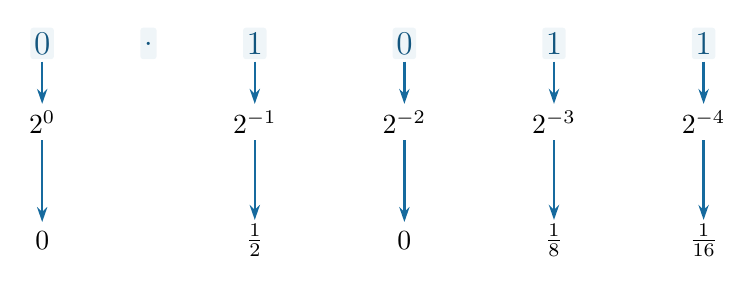
\begin{tikzpicture}[x=1mm,y=1mm]
\node[vc digit] (d0) at (0,0) {$ 0 $};
\node[vcnum] (w0) at (0,-10) {$ 2^{0} $};
\node[vcnum] (v0) at (0,-25) {$ 0 $};
\draw[vc arrow] (d0.south)--(w0.north);
\draw[vc arrow] (w0.south)--(v0.north);
\node[vc digit] (d1) at (27,0) {$ 1 $};
\node[vcnum] (w1) at (27,-10) {$ 2^{-1} $};
\node[vcnum] (v1) at (27,-25) {$ \frac{1}{2} $};
\draw[vc arrow] (d1.south)--(w1.north);
\draw[vc arrow] (w1.south)--(v1.north);
\node[vc digit] (d2) at (46,0) {$ 0 $};
\node[vcnum] (w2) at (46,-10) {$ 2^{-2} $};
\node[vcnum] (v2) at (46,-25) {$ 0 $};
\draw[vc arrow] (d2.south)--(w2.north);
\draw[vc arrow] (w2.south)--(v2.north);
\node[vc digit] (d3) at (65,0) {$ 1 $};
\node[vcnum] (w3) at (65,-10) {$ 2^{-3} $};
\node[vcnum] (v3) at (65,-25) {$ \frac{1}{8} $};
\draw[vc arrow] (d3.south)--(w3.north);
\draw[vc arrow] (w3.south)--(v3.north);
\node[vc digit] (d4) at (84,0) {$ 1 $};
\node[vcnum] (w4) at (84,-10) {$ 2^{-4} $};
\node[vcnum] (v4) at (84,-25) {$ \frac{1}{16} $};
\draw[vc arrow] (d4.south)--(w4.north);
\draw[vc arrow] (w4.south)--(v4.north);
\node[vc digit] at (13.5,0) {$.$};
\end{tikzpicture}\end{chThreeDiagram}
\end{minipage}\par

\[\begin{aligned}V&=0\times 2^{0}+1\times 2^{-1}+0\times 2^{-2}+1\times 2^{-3}+1\times 2^{-4}\\&=\frac{1}{2}+\frac{1}{8}+\frac{1}{16}=0.6875.\end{aligned}\]
\[\therefore\ (0.1011)_{2}=(0.6875)_{10}.\]
\end{minipage}\par
\par\noindent\begin{minipage}{\linewidth}
\convExample{৩}{মিশ্র সংখ্যা}
$ (110101.011)_{2} $-কে ১০ ভিত্তিতে রূপান্তর করো।\par
\par\noindent\begin{minipage}{\linewidth}\centering
\phantomsection\label{VC019}
\begin{chThreeDiagram}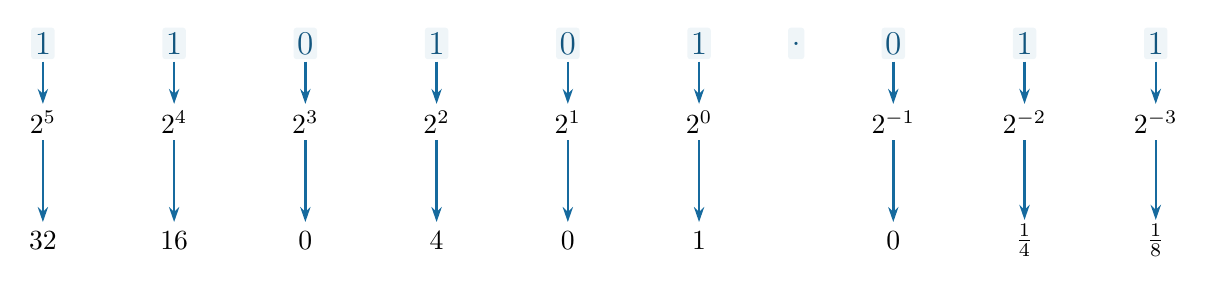
\begin{tikzpicture}[x=1mm,y=1mm]
\node[vc digit] (d0) at (0.0,0) {$ 1 $};
\node[vcnum] (w0) at (0.0,-10) {$ 2^{5} $};
\node[vcnum] (v0) at (0.0,-25) {$ 32 $};
\draw[vc arrow] (d0.south)--(w0.north);
\draw[vc arrow] (w0.south)--(v0.north);
\node[vc digit] (d1) at (16.666666666666668,0) {$ 1 $};
\node[vcnum] (w1) at (16.666666666666668,-10) {$ 2^{4} $};
\node[vcnum] (v1) at (16.666666666666668,-25) {$ 16 $};
\draw[vc arrow] (d1.south)--(w1.north);
\draw[vc arrow] (w1.south)--(v1.north);
\node[vc digit] (d2) at (33.333333333333336,0) {$ 0 $};
\node[vcnum] (w2) at (33.333333333333336,-10) {$ 2^{3} $};
\node[vcnum] (v2) at (33.333333333333336,-25) {$ 0 $};
\draw[vc arrow] (d2.south)--(w2.north);
\draw[vc arrow] (w2.south)--(v2.north);
\node[vc digit] (d3) at (50.0,0) {$ 1 $};
\node[vcnum] (w3) at (50.0,-10) {$ 2^{2} $};
\node[vcnum] (v3) at (50.0,-25) {$ 4 $};
\draw[vc arrow] (d3.south)--(w3.north);
\draw[vc arrow] (w3.south)--(v3.north);
\node[vc digit] (d4) at (66.66666666666667,0) {$ 0 $};
\node[vcnum] (w4) at (66.66666666666667,-10) {$ 2^{1} $};
\node[vcnum] (v4) at (66.66666666666667,-25) {$ 0 $};
\draw[vc arrow] (d4.south)--(w4.north);
\draw[vc arrow] (w4.south)--(v4.north);
\node[vc digit] (d5) at (83.33333333333334,0) {$ 1 $};
\node[vcnum] (w5) at (83.33333333333334,-10) {$ 2^{0} $};
\node[vcnum] (v5) at (83.33333333333334,-25) {$ 1 $};
\draw[vc arrow] (d5.south)--(w5.north);
\draw[vc arrow] (w5.south)--(v5.north);
\node[vc digit] (d6) at (108.0,0) {$ 0 $};
\node[vcnum] (w6) at (108.0,-10) {$ 2^{-1} $};
\node[vcnum] (v6) at (108.0,-25) {$ 0 $};
\draw[vc arrow] (d6.south)--(w6.north);
\draw[vc arrow] (w6.south)--(v6.north);
\node[vc digit] (d7) at (124.66666666666667,0) {$ 1 $};
\node[vcnum] (w7) at (124.66666666666667,-10) {$ 2^{-2} $};
\node[vcnum] (v7) at (124.66666666666667,-25) {$ \frac{1}{4} $};
\draw[vc arrow] (d7.south)--(w7.north);
\draw[vc arrow] (w7.south)--(v7.north);
\node[vc digit] (d8) at (141.33333333333334,0) {$ 1 $};
\node[vcnum] (w8) at (141.33333333333334,-10) {$ 2^{-3} $};
\node[vcnum] (v8) at (141.33333333333334,-25) {$ \frac{1}{8} $};
\draw[vc arrow] (d8.south)--(w8.north);
\draw[vc arrow] (w8.south)--(v8.north);
\node[vc digit] at (95.66666666666667,0) {$.$};
\end{tikzpicture}\end{chThreeDiagram}
\end{minipage}\par

\[\begin{aligned}V&=1\times 2^{5}+1\times 2^{4}+0\times 2^{3}+1\times 2^{2}+0\times 2^{1}+1\times 2^{0}+0\times 2^{-1}+1\times 2^{-2}+1\times 2^{-3}\\&=32+16+4+1+\frac{1}{4}+\frac{1}{8}=53.375.\end{aligned}\]
\[\therefore\ (110101.011)_{2}=(53.375)_{10}.\]
\end{minipage}\par


\smallhead{অক্টালের সঙ্গে দশমিক ও বাইনারি}
\subsection{দশমিক থেকে অক্টাল}
পূর্ণাংশে লক্ষ্য ভিত্তি দিয়ে ভাগ করো; ভাগশেষ নিচ থেকে ওপরে পড়ো। ভগ্নাংশে একই ভিত্তি দিয়ে গুণ করে পাওয়া অঙ্ক ওপর থেকে নিচে পড়ো।
\par\noindent\begin{minipage}{\linewidth}
\convExample{১}{পূর্ণসংখ্যা}
$ (173)_{10} $-কে ৮ ভিত্তিতে রূপান্তর করো।\par
\par\noindent\begin{minipage}{\linewidth}\centering
\phantomsection\label{VC005}
\begin{chThreeDiagram}\begin{tikzpicture}[x=1mm,y=1mm]
\path[use as bounding box] (-3,9) rectangle (72,-35);
\node[vcnote] at (15,7) {ভাজ্য/ভাগফল};
\node[vcnote] at (44,7) {ভাগশেষ};
\node[vcnum] at (0.0,0) {$ 8 $};
\node[vcnum] at (10.0,0) {$ 173 $};
\draw[vc line] (5.0,3)--(5.0,-3.5)--(50,-3.5);
\node[vcnum] (r0) at (44,-7) {$ 5 $};
\node[vcnum] at (1.5,-7) {$ 8 $};
\node[vcnum] at (11.5,-7) {$ 21 $};
\draw[vc line] (6.5,-4)--(6.5,-10.5)--(50,-10.5);
\node[vcnum] (r1) at (44,-14) {$ 5 $};
\node[vcnum] at (3.0,-14) {$ 8 $};
\node[vcnum] at (13.0,-14) {$ 2 $};
\draw[vc line] (8.0,-11)--(8.0,-17.5)--(50,-17.5);
\node[vcnum] (r2) at (44,-21) {$ 2 $};
\node[vcnum] at (14.5,-21) {$0$};
\node[vcnote] at (61,-3) {LSB};
\node[vcnote] at (61,-26) {MSB};
\draw[vc arrow] (61,-21)--(61,-7);
\node[vcnote] at (31,-33) {নিচ থেকে ওপরে পড়ো};
\end{tikzpicture}\end{chThreeDiagram}
\end{minipage}\par
\[\therefore\ (173)_{10}=(255)_{8}.\]
\end{minipage}\par
\par\noindent\begin{minipage}{\linewidth}
\convExample{২}{শুধু ভগ্নাংশ}
$ (0.046875)_{10} $-কে ৮ ভিত্তিতে রূপান্তর করো।\par
\par\noindent\begin{minipage}{\linewidth}\centering
\phantomsection\label{VC006}
\begin{chThreeDiagram}\begin{tikzpicture}[x=1mm,y=1mm]
\path[use as bounding box] (-9,9) rectangle (76,-39);
\node[vcnote] at (14,7) {প্রাপ্ত অঙ্ক};
\node[vcnote] at (45,7) {ভগ্নাংশ};
\node[vcnum] at (45,0) {$ 0.046875 $};
\draw[vc line] (26,3)--(26,-27);
\node[vcnum] (m0) at (45,-5) {$\times 8$};
\draw[vc line] (7,-8)--(65,-8);
\node[vcnum] at (14,-12) {$ 0 $};
\node[vcnum] (f0) at (45,-12) {$ 0.375 $};
\node[vcnum] (m1) at (45,-17) {$\times 8$};
\draw[vc line] (7,-20)--(65,-20);
\node[vcnum] at (14,-24) {$ 3 $};
\node[vcnum] (f1) at (45,-24) {$ 0 $};
\draw[vc arrow] (f0.east)--(72,-12)--(72,-17)--(m1.east);
\node[vcnote] at (0,-8) {MSB};
\node[vcnote] at (0,-29) {LSB};
\draw[vc arrow] (0,-12)--(0,-24);
\node[vcnote] at (34,-36) {ওপর থেকে নিচে পড়ো};
\end{tikzpicture}\end{chThreeDiagram}
\end{minipage}\par
\[\therefore\ (0.046875)_{10}=(0.03)_{8}.\]
\end{minipage}\par
\par\noindent\begin{minipage}{\linewidth}
\convExample{৩}{মিশ্র সংখ্যা}
$ (218.625)_{10} $-কে ৮ ভিত্তিতে রূপান্তর করো।\par
\begin{minipage}[t]{.48\linewidth}\vspace{0pt}\centering\textbf{পূর্ণাংশ}\par\vspace{1mm}
\par\noindent\begin{minipage}{\linewidth}\centering
\phantomsection\label{VC007}
\begin{chThreeDiagram}\begin{tikzpicture}[x=1mm,y=1mm]
\path[use as bounding box] (-3,9) rectangle (72,-35);
\node[vcnote] at (15,7) {ভাজ্য/ভাগফল};
\node[vcnote] at (44,7) {ভাগশেষ};
\node[vcnum] at (0.0,0) {$ 8 $};
\node[vcnum] at (10.0,0) {$ 218 $};
\draw[vc line] (5.0,3)--(5.0,-3.5)--(50,-3.5);
\node[vcnum] (r0) at (44,-7) {$ 2 $};
\node[vcnum] at (1.5,-7) {$ 8 $};
\node[vcnum] at (11.5,-7) {$ 27 $};
\draw[vc line] (6.5,-4)--(6.5,-10.5)--(50,-10.5);
\node[vcnum] (r1) at (44,-14) {$ 3 $};
\node[vcnum] at (3.0,-14) {$ 8 $};
\node[vcnum] at (13.0,-14) {$ 3 $};
\draw[vc line] (8.0,-11)--(8.0,-17.5)--(50,-17.5);
\node[vcnum] (r2) at (44,-21) {$ 3 $};
\node[vcnum] at (14.5,-21) {$0$};
\node[vcnote] at (61,-3) {LSB};
\node[vcnote] at (61,-26) {MSB};
\draw[vc arrow] (61,-21)--(61,-7);
\node[vcnote] at (31,-33) {নিচ থেকে ওপরে পড়ো};
\end{tikzpicture}\end{chThreeDiagram}
\end{minipage}\par

$ (332)_{8} $
\end{minipage}\hfill
\begin{minipage}[t]{.48\linewidth}\vspace{0pt}\centering\textbf{ভগ্নাংশ}\par\vspace{1mm}
\par\noindent\begin{minipage}{\linewidth}\centering
\phantomsection\label{VC008}
\begin{chThreeDiagram}\begin{tikzpicture}[x=1mm,y=1mm]
\path[use as bounding box] (-9,9) rectangle (76,-27);
\node[vcnote] at (14,7) {প্রাপ্ত অঙ্ক};
\node[vcnote] at (45,7) {ভগ্নাংশ};
\node[vcnum] at (45,0) {$ 0.625 $};
\draw[vc line] (26,3)--(26,-15);
\node[vcnum] (m0) at (45,-5) {$\times 8$};
\draw[vc line] (7,-8)--(65,-8);
\node[vcnum] at (14,-12) {$ 5 $};
\node[vcnum] (f0) at (45,-12) {$ 0 $};
\node[vcnote] at (0,-10) {MSB=LSB};
\draw[vc arrow] (0,-14)--(0,-20);
\node[vcnote] at (34,-24) {ওপর থেকে নিচে পড়ো};
\end{tikzpicture}\end{chThreeDiagram}
\end{minipage}\par

$ (0.5)_{8} $
\end{minipage}\par
\[\therefore\ (218.625)_{10}=(332.5)_{8}.\]
\end{minipage}\par

\subsection{অক্টাল থেকে দশমিক}
বিন্দুর বামে ওজন $b^0,b^1,\ldots$; ডানে $b^{-1},b^{-2},\ldots$। প্রতিটি অঙ্কের সঙ্গে তার ওজন গুণ করে অবদানগুলো যোগ করো।
\par\noindent\begin{minipage}{\linewidth}
\convExample{১}{পূর্ণসংখ্যা}
$ (275)_{8} $-কে ১০ ভিত্তিতে রূপান্তর করো।\par
\par\noindent\begin{minipage}{\linewidth}\centering
\phantomsection\label{VC033}
\begin{chThreeDiagram}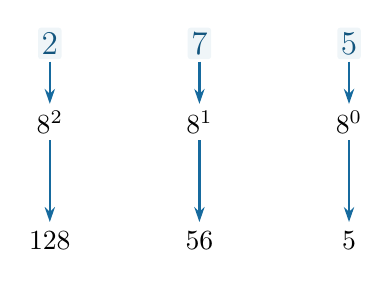
\begin{tikzpicture}[x=1mm,y=1mm]
\node[vc digit] (d0) at (0,0) {$ 2 $};
\node[vcnum] (w0) at (0,-10) {$ 8^{2} $};
\node[vcnum] (v0) at (0,-25) {$ 128 $};
\draw[vc arrow] (d0.south)--(w0.north);
\draw[vc arrow] (w0.south)--(v0.north);
\node[vc digit] (d1) at (19,0) {$ 7 $};
\node[vcnum] (w1) at (19,-10) {$ 8^{1} $};
\node[vcnum] (v1) at (19,-25) {$ 56 $};
\draw[vc arrow] (d1.south)--(w1.north);
\draw[vc arrow] (w1.south)--(v1.north);
\node[vc digit] (d2) at (38,0) {$ 5 $};
\node[vcnum] (w2) at (38,-10) {$ 8^{0} $};
\node[vcnum] (v2) at (38,-25) {$ 5 $};
\draw[vc arrow] (d2.south)--(w2.north);
\draw[vc arrow] (w2.south)--(v2.north);
\end{tikzpicture}\end{chThreeDiagram}
\end{minipage}\par

\[\begin{aligned}V&=2\times 8^{2}+7\times 8^{1}+5\times 8^{0}\\&=128+56+5=189.\end{aligned}\]
\[\therefore\ (275)_{8}=(189)_{10}.\]
\end{minipage}\par
\par\noindent\begin{minipage}{\linewidth}
\convExample{২}{শুধু ভগ্নাংশ}
$ (0.47)_{8} $-কে ১০ ভিত্তিতে রূপান্তর করো।\par
\par\noindent\begin{minipage}{\linewidth}\centering
\phantomsection\label{VC034}
\begin{chThreeDiagram}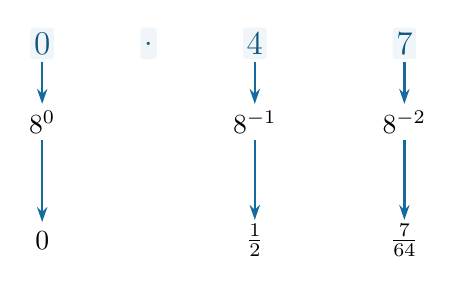
\begin{tikzpicture}[x=1mm,y=1mm]
\node[vc digit] (d0) at (0,0) {$ 0 $};
\node[vcnum] (w0) at (0,-10) {$ 8^{0} $};
\node[vcnum] (v0) at (0,-25) {$ 0 $};
\draw[vc arrow] (d0.south)--(w0.north);
\draw[vc arrow] (w0.south)--(v0.north);
\node[vc digit] (d1) at (27,0) {$ 4 $};
\node[vcnum] (w1) at (27,-10) {$ 8^{-1} $};
\node[vcnum] (v1) at (27,-25) {$ \frac{1}{2} $};
\draw[vc arrow] (d1.south)--(w1.north);
\draw[vc arrow] (w1.south)--(v1.north);
\node[vc digit] (d2) at (46,0) {$ 7 $};
\node[vcnum] (w2) at (46,-10) {$ 8^{-2} $};
\node[vcnum] (v2) at (46,-25) {$ \frac{7}{64} $};
\draw[vc arrow] (d2.south)--(w2.north);
\draw[vc arrow] (w2.south)--(v2.north);
\node[vc digit] at (13.5,0) {$.$};
\end{tikzpicture}\end{chThreeDiagram}
\end{minipage}\par

\[\begin{aligned}V&=0\times 8^{0}+4\times 8^{-1}+7\times 8^{-2}\\&=\frac{1}{2}+\frac{7}{64}=0.609375.\end{aligned}\]
\[\therefore\ (0.47)_{8}=(0.609375)_{10}.\]
\end{minipage}\par
\par\noindent\begin{minipage}{\linewidth}
\convExample{৩}{মিশ্র সংখ্যা}
$ (356.24)_{8} $-কে ১০ ভিত্তিতে রূপান্তর করো।\par
\par\noindent\begin{minipage}{\linewidth}\centering
\phantomsection\label{VC035}
\begin{chThreeDiagram}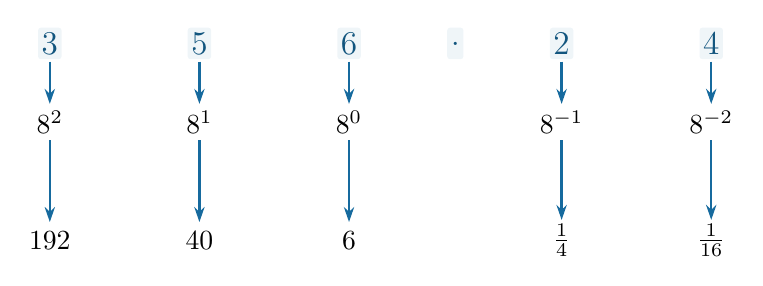
\begin{tikzpicture}[x=1mm,y=1mm]
\node[vc digit] (d0) at (0,0) {$ 3 $};
\node[vcnum] (w0) at (0,-10) {$ 8^{2} $};
\node[vcnum] (v0) at (0,-25) {$ 192 $};
\draw[vc arrow] (d0.south)--(w0.north);
\draw[vc arrow] (w0.south)--(v0.north);
\node[vc digit] (d1) at (19,0) {$ 5 $};
\node[vcnum] (w1) at (19,-10) {$ 8^{1} $};
\node[vcnum] (v1) at (19,-25) {$ 40 $};
\draw[vc arrow] (d1.south)--(w1.north);
\draw[vc arrow] (w1.south)--(v1.north);
\node[vc digit] (d2) at (38,0) {$ 6 $};
\node[vcnum] (w2) at (38,-10) {$ 8^{0} $};
\node[vcnum] (v2) at (38,-25) {$ 6 $};
\draw[vc arrow] (d2.south)--(w2.north);
\draw[vc arrow] (w2.south)--(v2.north);
\node[vc digit] (d3) at (65,0) {$ 2 $};
\node[vcnum] (w3) at (65,-10) {$ 8^{-1} $};
\node[vcnum] (v3) at (65,-25) {$ \frac{1}{4} $};
\draw[vc arrow] (d3.south)--(w3.north);
\draw[vc arrow] (w3.south)--(v3.north);
\node[vc digit] (d4) at (84,0) {$ 4 $};
\node[vcnum] (w4) at (84,-10) {$ 8^{-2} $};
\node[vcnum] (v4) at (84,-25) {$ \frac{1}{16} $};
\draw[vc arrow] (d4.south)--(w4.north);
\draw[vc arrow] (w4.south)--(v4.north);
\node[vc digit] at (51.5,0) {$.$};
\end{tikzpicture}\end{chThreeDiagram}
\end{minipage}\par

\[\begin{aligned}V&=3\times 8^{2}+5\times 8^{1}+6\times 8^{0}+2\times 8^{-1}+4\times 8^{-2}\\&=192+40+6+\frac{1}{4}+\frac{1}{16}=238.3125.\end{aligned}\]
\[\therefore\ (356.24)_{8}=(238.3125)_{10}.\]
\end{minipage}\par

\subsection{অক্টাল থেকে বাইনারি}
প্রতি অক্টাল অঙ্কে ৩ বিট, প্রতি হেক্সাডেসিমাল অঙ্কে ৪ বিট। প্রতিটি অঙ্কের বিটগুলো একই ক্রমে একত্র করো; ভগ্নাংশের শুরুর শূন্য বাদ দিও না।
\par\noindent\begin{minipage}{\linewidth}
\convExample{১}{পূর্ণসংখ্যা}
$ (265)_{8} $-কে ২ ভিত্তিতে রূপান্তর করো।\par
\par\noindent\begin{minipage}{\linewidth}\centering
\phantomsection\label{VC036}
\begin{chThreeDiagram}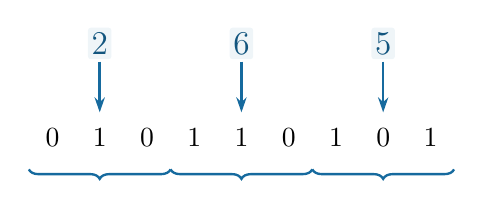
\begin{tikzpicture}[x=1mm,y=1mm]
\node[vc digit] (s0) at (6.0,0) {$ 2 $};
\draw[vc arrow] (s0.south)--(6.0,-9);
\node[vc digit] (s1) at (24.0,0) {$ 6 $};
\draw[vc arrow] (s1.south)--(24.0,-9);
\node[vc digit] (s2) at (42.0,0) {$ 5 $};
\draw[vc arrow] (s2.south)--(42.0,-9);
\node[vc bit] (raw0) at (0,-12) {$ 0 $};
\node[vc bit] (raw1) at (6,-12) {$ 1 $};
\node[vc bit] (raw2) at (12,-12) {$ 0 $};
\node[vc bit] (raw3) at (18,-12) {$ 1 $};
\node[vc bit] (raw4) at (24,-12) {$ 1 $};
\node[vc bit] (raw5) at (30,-12) {$ 0 $};
\node[vc bit] (raw6) at (36,-12) {$ 1 $};
\node[vc bit] (raw7) at (42,-12) {$ 0 $};
\node[vc bit] (raw8) at (48,-12) {$ 1 $};
\draw[vc brace] (-3.0,-16)--(15.0,-16);
\draw[vc brace] (15.0,-16)--(33.0,-16);
\draw[vc brace] (33.0,-16)--(51.0,-16);
\end{tikzpicture}\end{chThreeDiagram}
\end{minipage}\par
\[\therefore\ (265)_{8}=(10110101)_{2}.\]
পূর্ণাংশের শুরুর বা ভগ্নাংশের শেষের অপ্রয়োজনীয় ০ বাদ দিয়ে ফল লেখা হয়েছে; ভগ্নাংশের শুরুর ০ বাদ যায় না।\par
\end{minipage}\par
\par\noindent\begin{minipage}{\linewidth}
\convExample{২}{শুধু ভগ্নাংশ}
$ (0.47)_{8} $-কে ২ ভিত্তিতে রূপান্তর করো।\par
\par\noindent\begin{minipage}{\linewidth}\centering
\phantomsection\label{VC037}
\begin{chThreeDiagram}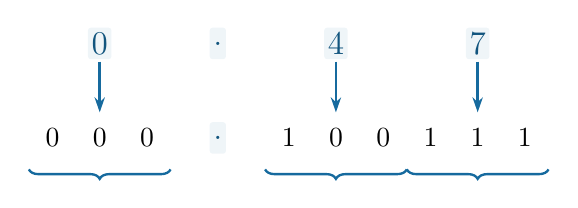
\begin{tikzpicture}[x=1mm,y=1mm]
\node[vc digit] (s0) at (6.0,0) {$ 0 $};
\draw[vc arrow] (s0.south)--(6.0,-9);
\node[vc digit] (s1) at (36.0,0) {$ 4 $};
\draw[vc arrow] (s1.south)--(36.0,-9);
\node[vc digit] (s2) at (54.0,0) {$ 7 $};
\draw[vc arrow] (s2.south)--(54.0,-9);
\node[vc digit] at (21.0,0) {$.$};
\node[vc bit] (raw0) at (0,-12) {$ 0 $};
\node[vc bit] (raw1) at (6,-12) {$ 0 $};
\node[vc bit] (raw2) at (12,-12) {$ 0 $};
\node[vc bit] (raw3) at (30.0,-12) {$ 1 $};
\node[vc bit] (raw4) at (36.0,-12) {$ 0 $};
\node[vc bit] (raw5) at (42.0,-12) {$ 0 $};
\node[vc bit] (raw6) at (48.0,-12) {$ 1 $};
\node[vc bit] (raw7) at (54.0,-12) {$ 1 $};
\node[vc bit] (raw8) at (60.0,-12) {$ 1 $};
\node[vc digit] at (21.0,-12) {$.$};
\draw[vc brace] (-3.0,-16)--(15.0,-16);
\draw[vc brace] (27.0,-16)--(45.0,-16);
\draw[vc brace] (45.0,-16)--(63.0,-16);
\end{tikzpicture}\end{chThreeDiagram}
\end{minipage}\par
\[\therefore\ (0.47)_{8}=(0.100111)_{2}.\]
পূর্ণাংশের শুরুর বা ভগ্নাংশের শেষের অপ্রয়োজনীয় ০ বাদ দিয়ে ফল লেখা হয়েছে; ভগ্নাংশের শুরুর ০ বাদ যায় না।\par
\end{minipage}\par
\par\noindent\begin{minipage}{\linewidth}
\convExample{৩}{মিশ্র সংখ্যা}
$ (143.52)_{8} $-কে ২ ভিত্তিতে রূপান্তর করো।\par
\par\noindent\begin{minipage}{\linewidth}\centering
\phantomsection\label{VC038}
\begin{chThreeDiagram}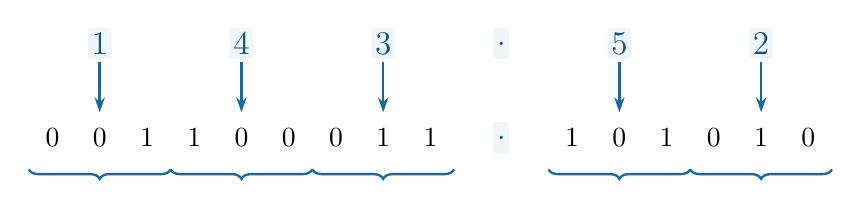
\begin{tikzpicture}[x=1mm,y=1mm]
\node[vc digit] (s0) at (6.0,0) {$ 1 $};
\draw[vc arrow] (s0.south)--(6.0,-9);
\node[vc digit] (s1) at (24.0,0) {$ 4 $};
\draw[vc arrow] (s1.south)--(24.0,-9);
\node[vc digit] (s2) at (42.0,0) {$ 3 $};
\draw[vc arrow] (s2.south)--(42.0,-9);
\node[vc digit] (s3) at (72.0,0) {$ 5 $};
\draw[vc arrow] (s3.south)--(72.0,-9);
\node[vc digit] (s4) at (90.0,0) {$ 2 $};
\draw[vc arrow] (s4.south)--(90.0,-9);
\node[vc digit] at (57.0,0) {$.$};
\node[vc bit] (raw0) at (0,-12) {$ 0 $};
\node[vc bit] (raw1) at (6,-12) {$ 0 $};
\node[vc bit] (raw2) at (12,-12) {$ 1 $};
\node[vc bit] (raw3) at (18,-12) {$ 1 $};
\node[vc bit] (raw4) at (24,-12) {$ 0 $};
\node[vc bit] (raw5) at (30,-12) {$ 0 $};
\node[vc bit] (raw6) at (36,-12) {$ 0 $};
\node[vc bit] (raw7) at (42,-12) {$ 1 $};
\node[vc bit] (raw8) at (48,-12) {$ 1 $};
\node[vc bit] (raw9) at (66.0,-12) {$ 1 $};
\node[vc bit] (raw10) at (72.0,-12) {$ 0 $};
\node[vc bit] (raw11) at (78.0,-12) {$ 1 $};
\node[vc bit] (raw12) at (84.0,-12) {$ 0 $};
\node[vc bit] (raw13) at (90.0,-12) {$ 1 $};
\node[vc bit] (raw14) at (96.0,-12) {$ 0 $};
\node[vc digit] at (57.0,-12) {$.$};
\draw[vc brace] (-3.0,-16)--(15.0,-16);
\draw[vc brace] (15.0,-16)--(33.0,-16);
\draw[vc brace] (33.0,-16)--(51.0,-16);
\draw[vc brace] (63.0,-16)--(81.0,-16);
\draw[vc brace] (81.0,-16)--(99.0,-16);
\end{tikzpicture}\end{chThreeDiagram}
\end{minipage}\par
\[\therefore\ (143.52)_{8}=(1100011.10101)_{2}.\]
পূর্ণাংশের শুরুর বা ভগ্নাংশের শেষের অপ্রয়োজনীয় ০ বাদ দিয়ে ফল লেখা হয়েছে; ভগ্নাংশের শুরুর ০ বাদ যায় না।\par
\end{minipage}\par

\subsection{বাইনারি থেকে অক্টাল}
বিন্দুর দুই পাশ আলাদা করে ৩ বিটের গ্রুপ করো। প্রয়োজনের শূন্য পূর্ণাংশের বামে ও ভগ্নাংশের ডানে বসে।
\par\noindent\begin{minipage}{\linewidth}
\convExample{১}{পূর্ণসংখ্যা}
$ (1101101)_{2} $-কে ৮ ভিত্তিতে রূপান্তর করো।\par
\par\noindent\begin{minipage}{\linewidth}\centering
\phantomsection\label{VC020}
\begin{chThreeDiagram}\begin{tikzpicture}[x=1mm,y=1mm]
\node[vc bit] (raw0) at (12,0) {$ 1 $};
\node[vc bit] (raw1) at (18,0) {$ 1 $};
\node[vc bit] (raw2) at (24,0) {$ 0 $};
\node[vc bit] (raw3) at (30,0) {$ 1 $};
\node[vc bit] (raw4) at (36,0) {$ 1 $};
\node[vc bit] (raw5) at (42,0) {$ 0 $};
\node[vc bit] (raw6) at (48,0) {$ 1 $};
\node[vc bit] (new0) at (0,-20) {$ 0 $};
\node[vc bit] (new1) at (6,-20) {$ 0 $};
\node[vc bit] (new2) at (12,-20) {$ 1 $};
\node[vc bit] (new3) at (18,-20) {$ 1 $};
\node[vc bit] (new4) at (24,-20) {$ 0 $};
\node[vc bit] (new5) at (30,-20) {$ 1 $};
\node[vc bit] (new6) at (36,-20) {$ 1 $};
\node[vc bit] (new7) at (42,-20) {$ 0 $};
\node[vc bit] (new8) at (48,-20) {$ 1 $};
\draw[vc arrow,draw=vcBlue!65] (raw0.south)--(12,-17);
\draw[vc arrow,draw=vcBlue!65] (raw1.south)--(18,-17);
\draw[vc arrow,draw=vcBlue!65] (raw2.south)--(24,-17);
\draw[vc arrow,draw=vcBlue!65] (raw3.south)--(30,-17);
\draw[vc arrow,draw=vcBlue!65] (raw4.south)--(36,-17);
\draw[vc arrow,draw=vcBlue!65] (raw5.south)--(42,-17);
\draw[vc arrow,draw=vcBlue!65] (raw6.south)--(48,-17);
\draw[dashed,draw=vcPad,line width=.85pt] (-2.5,-22.8) rectangle (8.5,-17.2);
\node[vcnote,text=vcPad,fill=vcPad!8,inner sep=1.5pt] (pad-left) at (-13.5,-9) {বামে ২টি ০};
\draw[vc arrow,draw=vcPad] (pad-left.south)--(3.0,-17);
\draw[vc brace] (-3.0,-24)--(15.0,-24);
\node[vc result] (g0) at (6.0,-37) {$ 1 $};
\draw[vc arrow] (6.0,-27)--(g0.north);
\draw[vc brace] (15.0,-24)--(33.0,-24);
\node[vc result] (g1) at (24.0,-37) {$ 5 $};
\draw[vc arrow] (24.0,-27)--(g1.north);
\draw[vc brace] (33.0,-24)--(51.0,-24);
\node[vc result] (g2) at (42.0,-37) {$ 5 $};
\draw[vc arrow] (42.0,-27)--(g2.north);
\end{tikzpicture}\end{chThreeDiagram}
\end{minipage}\par
\[\therefore\ (1101101)_{2}=(155)_{8}.\]
দাগঘেরা বিটগুলো গ্রুপ পূরণের জন্য যোগ করা শূন্য; এগুলো মান বদলায়নি।\par
\end{minipage}\par
\par\noindent\begin{minipage}{\linewidth}
\convExample{২}{শুধু ভগ্নাংশ}
$ (0.10111)_{2} $-কে ৮ ভিত্তিতে রূপান্তর করো।\par
\par\noindent\begin{minipage}{\linewidth}\centering
\phantomsection\label{VC021}
\begin{chThreeDiagram}\begin{tikzpicture}[x=1mm,y=1mm]
\node[vc digit] at (21.0,0) {$.$};
\node[vc bit] (raw0) at (12,0) {$ 0 $};
\node[vc bit] (raw1) at (30.0,0) {$ 1 $};
\node[vc bit] (raw2) at (36.0,0) {$ 0 $};
\node[vc bit] (raw3) at (42.0,0) {$ 1 $};
\node[vc bit] (raw4) at (48.0,0) {$ 1 $};
\node[vc bit] (raw5) at (54.0,0) {$ 1 $};
\node[vc bit] (new0) at (0,-20) {$ 0 $};
\node[vc bit] (new1) at (6,-20) {$ 0 $};
\node[vc bit] (new2) at (12,-20) {$ 0 $};
\node[vc bit] (new3) at (30.0,-20) {$ 1 $};
\node[vc bit] (new4) at (36.0,-20) {$ 0 $};
\node[vc bit] (new5) at (42.0,-20) {$ 1 $};
\node[vc bit] (new6) at (48.0,-20) {$ 1 $};
\node[vc bit] (new7) at (54.0,-20) {$ 1 $};
\node[vc bit] (new8) at (60.0,-20) {$ 0 $};
\draw[vc arrow,draw=vcBlue!65] (raw0.south)--(12,-17);
\draw[vc arrow,draw=vcBlue!65] (raw1.south)--(30.0,-17);
\draw[vc arrow,draw=vcBlue!65] (raw2.south)--(36.0,-17);
\draw[vc arrow,draw=vcBlue!65] (raw3.south)--(42.0,-17);
\draw[vc arrow,draw=vcBlue!65] (raw4.south)--(48.0,-17);
\draw[vc arrow,draw=vcBlue!65] (raw5.south)--(54.0,-17);
\node[vc digit] at (21.0,-20) {$.$};
\draw[dashed,draw=vcPad,line width=.85pt] (-2.5,-22.8) rectangle (8.5,-17.2);
\node[vcnote,text=vcPad,fill=vcPad!8,inner sep=1.5pt] (pad-left) at (-13.5,-9) {বামে ২টি ০};
\draw[vc arrow,draw=vcPad] (pad-left.south)--(3.0,-17);
\draw[dashed,draw=vcPad,line width=.85pt] (57.5,-22.8) rectangle (62.5,-17.2);
\node[vcnote,text=vcPad,fill=vcPad!8,inner sep=1.5pt] (pad-right) at (73.5,-9) {ডানে ১টি ০};
\draw[vc arrow,draw=vcPad] (pad-right.south)--(60.0,-17);
\draw[vc brace] (-3.0,-24)--(15.0,-24);
\node[vc result] (g0) at (6.0,-37) {$ 0 $};
\draw[vc arrow] (6.0,-27)--(g0.north);
\draw[vc brace] (27.0,-24)--(45.0,-24);
\node[vc result] (g1) at (36.0,-37) {$ 5 $};
\draw[vc arrow] (36.0,-27)--(g1.north);
\draw[vc brace] (45.0,-24)--(63.0,-24);
\node[vc result] (g2) at (54.0,-37) {$ 6 $};
\draw[vc arrow] (54.0,-27)--(g2.north);
\node[vc digit] at (21.0,-37) {$.$};
\end{tikzpicture}\end{chThreeDiagram}
\end{minipage}\par
\[\therefore\ (0.10111)_{2}=(0.56)_{8}.\]
দাগঘেরা বিটগুলো গ্রুপ পূরণের জন্য যোগ করা শূন্য; এগুলো মান বদলায়নি।\par
\end{minipage}\par
\par\noindent\begin{minipage}{\linewidth}
\convExample{৩}{মিশ্র সংখ্যা}
$ (101101.1101)_{2} $-কে ৮ ভিত্তিতে রূপান্তর করো।\par
\par\noindent\begin{minipage}{\linewidth}\centering
\phantomsection\label{VC022}
\begin{chThreeDiagram}\begin{tikzpicture}[x=1mm,y=1mm]
\node[vc digit] at (39.0,0) {$.$};
\node[vc bit] (raw0) at (0,0) {$ 1 $};
\node[vc bit] (raw1) at (6,0) {$ 0 $};
\node[vc bit] (raw2) at (12,0) {$ 1 $};
\node[vc bit] (raw3) at (18,0) {$ 1 $};
\node[vc bit] (raw4) at (24,0) {$ 0 $};
\node[vc bit] (raw5) at (30,0) {$ 1 $};
\node[vc bit] (raw6) at (48.0,0) {$ 1 $};
\node[vc bit] (raw7) at (54.0,0) {$ 1 $};
\node[vc bit] (raw8) at (60.0,0) {$ 0 $};
\node[vc bit] (raw9) at (66.0,0) {$ 1 $};
\node[vc bit] (new0) at (0,-20) {$ 1 $};
\node[vc bit] (new1) at (6,-20) {$ 0 $};
\node[vc bit] (new2) at (12,-20) {$ 1 $};
\node[vc bit] (new3) at (18,-20) {$ 1 $};
\node[vc bit] (new4) at (24,-20) {$ 0 $};
\node[vc bit] (new5) at (30,-20) {$ 1 $};
\node[vc bit] (new6) at (48.0,-20) {$ 1 $};
\node[vc bit] (new7) at (54.0,-20) {$ 1 $};
\node[vc bit] (new8) at (60.0,-20) {$ 0 $};
\node[vc bit] (new9) at (66.0,-20) {$ 1 $};
\node[vc bit] (new10) at (72.0,-20) {$ 0 $};
\node[vc bit] (new11) at (78.0,-20) {$ 0 $};
\draw[vc arrow,draw=vcBlue!65] (raw0.south)--(0,-17);
\draw[vc arrow,draw=vcBlue!65] (raw1.south)--(6,-17);
\draw[vc arrow,draw=vcBlue!65] (raw2.south)--(12,-17);
\draw[vc arrow,draw=vcBlue!65] (raw3.south)--(18,-17);
\draw[vc arrow,draw=vcBlue!65] (raw4.south)--(24,-17);
\draw[vc arrow,draw=vcBlue!65] (raw5.south)--(30,-17);
\draw[vc arrow,draw=vcBlue!65] (raw6.south)--(48.0,-17);
\draw[vc arrow,draw=vcBlue!65] (raw7.south)--(54.0,-17);
\draw[vc arrow,draw=vcBlue!65] (raw8.south)--(60.0,-17);
\draw[vc arrow,draw=vcBlue!65] (raw9.south)--(66.0,-17);
\node[vc digit] at (39.0,-20) {$.$};
\draw[dashed,draw=vcPad,line width=.85pt] (69.5,-22.8) rectangle (80.5,-17.2);
\node[vcnote,text=vcPad,fill=vcPad!8,inner sep=1.5pt] (pad-right) at (91.5,-9) {ডানে ২টি ০};
\draw[vc arrow,draw=vcPad] (pad-right.south)--(75.0,-17);
\draw[vc brace] (-3.0,-24)--(15.0,-24);
\node[vc result] (g0) at (6.0,-37) {$ 5 $};
\draw[vc arrow] (6.0,-27)--(g0.north);
\draw[vc brace] (15.0,-24)--(33.0,-24);
\node[vc result] (g1) at (24.0,-37) {$ 5 $};
\draw[vc arrow] (24.0,-27)--(g1.north);
\draw[vc brace] (45.0,-24)--(63.0,-24);
\node[vc result] (g2) at (54.0,-37) {$ 6 $};
\draw[vc arrow] (54.0,-27)--(g2.north);
\draw[vc brace] (63.0,-24)--(81.0,-24);
\node[vc result] (g3) at (72.0,-37) {$ 4 $};
\draw[vc arrow] (72.0,-27)--(g3.north);
\node[vc digit] at (39.0,-37) {$.$};
\end{tikzpicture}\end{chThreeDiagram}
\end{minipage}\par
\[\therefore\ (101101.1101)_{2}=(55.64)_{8}.\]
দাগঘেরা বিটগুলো গ্রুপ পূরণের জন্য যোগ করা শূন্য; এগুলো মান বদলায়নি।\par
\end{minipage}\par


\smallhead{হেক্সাডেসিমালের সঙ্গে দশমিক ও বাইনারি}
\subsection{হেক্সাডেসিমাল থেকে দশমিক}
বিন্দুর বামে ওজন $b^0,b^1,\ldots$; ডানে $b^{-1},b^{-2},\ldots$। প্রতিটি অঙ্কের সঙ্গে তার ওজন গুণ করে অবদানগুলো যোগ করো।
\par\noindent\begin{minipage}{\linewidth}
\convExample{১}{পূর্ণসংখ্যা}
$ (6DF)_{16} $-কে ১০ ভিত্তিতে রূপান্তর করো।\par
\par\noindent\begin{minipage}{\linewidth}\centering
\phantomsection\label{VC049}
\begin{chThreeDiagram}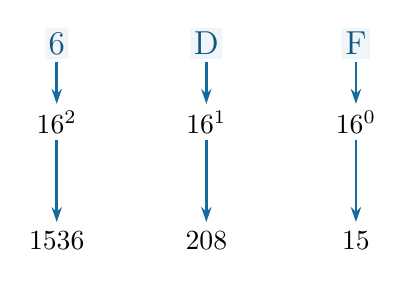
\begin{tikzpicture}[x=1mm,y=1mm]
\node[vc digit] (d0) at (0,0) {$ 6 $};
\node[vcnum] (w0) at (0,-10) {$ 16^{2} $};
\node[vcnum] (v0) at (0,-25) {$ 1536 $};
\draw[vc arrow] (d0.south)--(w0.north);
\draw[vc arrow] (w0.south)--(v0.north);
\node[vc digit] (d1) at (19,0) {$ \mathrm{D} $};
\node[vcnum] (w1) at (19,-10) {$ 16^{1} $};
\node[vcnum] (v1) at (19,-25) {$ 208 $};
\draw[vc arrow] (d1.south)--(w1.north);
\draw[vc arrow] (w1.south)--(v1.north);
\node[vc digit] (d2) at (38,0) {$ \mathrm{F} $};
\node[vcnum] (w2) at (38,-10) {$ 16^{0} $};
\node[vcnum] (v2) at (38,-25) {$ 15 $};
\draw[vc arrow] (d2.south)--(w2.north);
\draw[vc arrow] (w2.south)--(v2.north);
\end{tikzpicture}\end{chThreeDiagram}
\end{minipage}\par

\[\begin{aligned}V&=6\times 16^{2}+\mathrm{D}\times 16^{1}+\mathrm{F}\times 16^{0}\\&=1536+208+15=1759.\end{aligned}\]
\[\therefore\ (6DF)_{16}=(1759)_{10}.\]
\end{minipage}\par
\par\noindent\begin{minipage}{\linewidth}
\convExample{২}{শুধু ভগ্নাংশ}
$ (0.A6)_{16} $-কে ১০ ভিত্তিতে রূপান্তর করো।\par
\par\noindent\begin{minipage}{\linewidth}\centering
\phantomsection\label{VC050}
\begin{chThreeDiagram}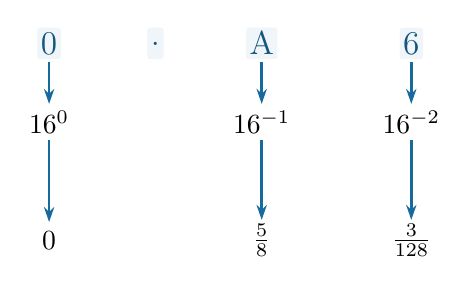
\begin{tikzpicture}[x=1mm,y=1mm]
\node[vc digit] (d0) at (0,0) {$ 0 $};
\node[vcnum] (w0) at (0,-10) {$ 16^{0} $};
\node[vcnum] (v0) at (0,-25) {$ 0 $};
\draw[vc arrow] (d0.south)--(w0.north);
\draw[vc arrow] (w0.south)--(v0.north);
\node[vc digit] (d1) at (27,0) {$ \mathrm{A} $};
\node[vcnum] (w1) at (27,-10) {$ 16^{-1} $};
\node[vcnum] (v1) at (27,-25) {$ \frac{5}{8} $};
\draw[vc arrow] (d1.south)--(w1.north);
\draw[vc arrow] (w1.south)--(v1.north);
\node[vc digit] (d2) at (46,0) {$ 6 $};
\node[vcnum] (w2) at (46,-10) {$ 16^{-2} $};
\node[vcnum] (v2) at (46,-25) {$ \frac{3}{128} $};
\draw[vc arrow] (d2.south)--(w2.north);
\draw[vc arrow] (w2.south)--(v2.north);
\node[vc digit] at (13.5,0) {$.$};
\end{tikzpicture}\end{chThreeDiagram}
\end{minipage}\par

\[\begin{aligned}V&=0\times 16^{0}+\mathrm{A}\times 16^{-1}+6\times 16^{-2}\\&=\frac{5}{8}+\frac{3}{128}=0.6484375.\end{aligned}\]
\[\therefore\ (0.A6)_{16}=(0.6484375)_{10}.\]
\end{minipage}\par
\par\noindent\begin{minipage}{\linewidth}
\convExample{৩}{মিশ্র সংখ্যা}
$ (3B.9C)_{16} $-কে ১০ ভিত্তিতে রূপান্তর করো।\par
\par\noindent\begin{minipage}{\linewidth}\centering
\phantomsection\label{VC051}
\begin{chThreeDiagram}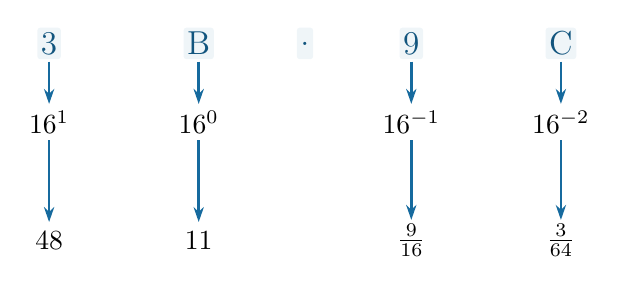
\begin{tikzpicture}[x=1mm,y=1mm]
\node[vc digit] (d0) at (0,0) {$ 3 $};
\node[vcnum] (w0) at (0,-10) {$ 16^{1} $};
\node[vcnum] (v0) at (0,-25) {$ 48 $};
\draw[vc arrow] (d0.south)--(w0.north);
\draw[vc arrow] (w0.south)--(v0.north);
\node[vc digit] (d1) at (19,0) {$ \mathrm{B} $};
\node[vcnum] (w1) at (19,-10) {$ 16^{0} $};
\node[vcnum] (v1) at (19,-25) {$ 11 $};
\draw[vc arrow] (d1.south)--(w1.north);
\draw[vc arrow] (w1.south)--(v1.north);
\node[vc digit] (d2) at (46,0) {$ 9 $};
\node[vcnum] (w2) at (46,-10) {$ 16^{-1} $};
\node[vcnum] (v2) at (46,-25) {$ \frac{9}{16} $};
\draw[vc arrow] (d2.south)--(w2.north);
\draw[vc arrow] (w2.south)--(v2.north);
\node[vc digit] (d3) at (65,0) {$ \mathrm{C} $};
\node[vcnum] (w3) at (65,-10) {$ 16^{-2} $};
\node[vcnum] (v3) at (65,-25) {$ \frac{3}{64} $};
\draw[vc arrow] (d3.south)--(w3.north);
\draw[vc arrow] (w3.south)--(v3.north);
\node[vc digit] at (32.5,0) {$.$};
\end{tikzpicture}\end{chThreeDiagram}
\end{minipage}\par

\[\begin{aligned}V&=3\times 16^{1}+\mathrm{B}\times 16^{0}+9\times 16^{-1}+\mathrm{C}\times 16^{-2}\\&=48+11+\frac{9}{16}+\frac{3}{64}=59.609375.\end{aligned}\]
\[\therefore\ (3B.9C)_{16}=(59.609375)_{10}.\]
\end{minipage}\par

\subsection{দশমিক থেকে হেক্সাডেসিমাল}
পূর্ণাংশে লক্ষ্য ভিত্তি দিয়ে ভাগ করো; ভাগশেষ নিচ থেকে ওপরে পড়ো। ভগ্নাংশে একই ভিত্তি দিয়ে গুণ করে পাওয়া অঙ্ক ওপর থেকে নিচে পড়ো।
হেক্সাডেসিমালে দশমিক ১০–১৫-এর অঙ্ক যথাক্রমে A–F; আগের mapping table দেখো।
\par\noindent\begin{minipage}{\linewidth}
\convExample{১}{পূর্ণসংখ্যা}
$ (345)_{10} $-কে ১৬ ভিত্তিতে রূপান্তর করো।\par
\par\noindent\begin{minipage}{\linewidth}\centering
\phantomsection\label{VC009}
\begin{chThreeDiagram}\begin{tikzpicture}[x=1mm,y=1mm]
\path[use as bounding box] (-3,9) rectangle (72,-35);
\node[vcnote] at (15,7) {ভাজ্য/ভাগফল};
\node[vcnote] at (44,7) {ভাগশেষ};
\node[vcnum] at (0.0,0) {$ 16 $};
\node[vcnum] at (10.0,0) {$ 345 $};
\draw[vc line] (5.0,3)--(5.0,-3.5)--(50,-3.5);
\node[vcnum] (r0) at (44,-7) {$ 9 $};
\node[vcnum] at (1.5,-7) {$ 16 $};
\node[vcnum] at (11.5,-7) {$ 21 $};
\draw[vc line] (6.5,-4)--(6.5,-10.5)--(50,-10.5);
\node[vcnum] (r1) at (44,-14) {$ 5 $};
\node[vcnum] at (3.0,-14) {$ 16 $};
\node[vcnum] at (13.0,-14) {$ 1 $};
\draw[vc line] (8.0,-11)--(8.0,-17.5)--(50,-17.5);
\node[vcnum] (r2) at (44,-21) {$ 1 $};
\node[vcnum] at (14.5,-21) {$0$};
\node[vcnote] at (61,-3) {LSB};
\node[vcnote] at (61,-26) {MSB};
\draw[vc arrow] (61,-21)--(61,-7);
\node[vcnote] at (31,-33) {নিচ থেকে ওপরে পড়ো};
\end{tikzpicture}\end{chThreeDiagram}
\end{minipage}\par
\[\therefore\ (345)_{10}=(159)_{16}.\]
\end{minipage}\par
\par\noindent\begin{minipage}{\linewidth}
\convExample{২}{শুধু ভগ্নাংশ}
$ (0.703125)_{10} $-কে ১৬ ভিত্তিতে রূপান্তর করো।\par
\par\noindent\begin{minipage}{\linewidth}\centering
\phantomsection\label{VC010}
\begin{chThreeDiagram}\begin{tikzpicture}[x=1mm,y=1mm]
\path[use as bounding box] (-9,9) rectangle (76,-39);
\node[vcnote] at (14,7) {প্রাপ্ত অঙ্ক};
\node[vcnote] at (45,7) {ভগ্নাংশ};
\node[vcnum] at (45,0) {$ 0.703125 $};
\draw[vc line] (26,3)--(26,-27);
\node[vcnum] (m0) at (45,-5) {$\times 16$};
\draw[vc line] (7,-8)--(65,-8);
\node[vcnum] at (14,-12) {$ \mathrm{B}\,( 11 ) $};
\node[vcnum] (f0) at (45,-12) {$ 0.25 $};
\node[vcnum] (m1) at (45,-17) {$\times 16$};
\draw[vc line] (7,-20)--(65,-20);
\node[vcnum] at (14,-24) {$ 4 $};
\node[vcnum] (f1) at (45,-24) {$ 0 $};
\draw[vc arrow] (f0.east)--(72,-12)--(72,-17)--(m1.east);
\node[vcnote] at (0,-8) {MSB};
\node[vcnote] at (0,-29) {LSB};
\draw[vc arrow] (0,-12)--(0,-24);
\node[vcnote] at (34,-36) {ওপর থেকে নিচে পড়ো};
\end{tikzpicture}\end{chThreeDiagram}
\end{minipage}\par
\[\therefore\ (0.703125)_{10}=(0.B4)_{16}.\]
\end{minipage}\par
\par\noindent\begin{minipage}{\linewidth}
\convExample{৩}{মিশ্র সংখ্যা}
$ (107.5703125)_{10} $-কে ১৬ ভিত্তিতে রূপান্তর করো।\par
\begin{minipage}[t]{.48\linewidth}\vspace{0pt}\centering\textbf{পূর্ণাংশ}\par\vspace{1mm}
\par\noindent\begin{minipage}{\linewidth}\centering
\phantomsection\label{VC011}
\begin{chThreeDiagram}\begin{tikzpicture}[x=1mm,y=1mm]
\path[use as bounding box] (-3,9) rectangle (72,-28);
\node[vcnote] at (15,7) {ভাজ্য/ভাগফল};
\node[vcnote] at (44,7) {ভাগশেষ};
\node[vcnum] at (0.0,0) {$ 16 $};
\node[vcnum] at (10.0,0) {$ 107 $};
\draw[vc line] (5.0,3)--(5.0,-3.5)--(50,-3.5);
\node[vcnum] (r0) at (44,-7) {$ \mathrm{B} $};
\node[vcnum] at (1.5,-7) {$ 16 $};
\node[vcnum] at (11.5,-7) {$ 6 $};
\draw[vc line] (6.5,-4)--(6.5,-10.5)--(50,-10.5);
\node[vcnum] (r1) at (44,-14) {$ 6 $};
\node[vcnum] at (13.0,-14) {$0$};
\node[vcnote] at (61,-3) {LSB};
\node[vcnote] at (61,-19) {MSB};
\draw[vc arrow] (61,-14)--(61,-7);
\node[vcnote] at (31,-26) {নিচ থেকে ওপরে পড়ো};
\end{tikzpicture}\end{chThreeDiagram}
\end{minipage}\par

$ (6B)_{16} $
\end{minipage}\hfill
\begin{minipage}[t]{.48\linewidth}\vspace{0pt}\centering\textbf{ভগ্নাংশ}\par\vspace{1mm}
\par\noindent\begin{minipage}{\linewidth}\centering
\phantomsection\label{VC012}
\begin{chThreeDiagram}\begin{tikzpicture}[x=1mm,y=1mm]
\path[use as bounding box] (-9,9) rectangle (76,-39);
\node[vcnote] at (14,7) {প্রাপ্ত অঙ্ক};
\node[vcnote] at (45,7) {ভগ্নাংশ};
\node[vcnum] at (45,0) {$ 0.5703125 $};
\draw[vc line] (26,3)--(26,-27);
\node[vcnum] (m0) at (45,-5) {$\times 16$};
\draw[vc line] (7,-8)--(65,-8);
\node[vcnum] at (14,-12) {$ 9 $};
\node[vcnum] (f0) at (45,-12) {$ 0.125 $};
\node[vcnum] (m1) at (45,-17) {$\times 16$};
\draw[vc line] (7,-20)--(65,-20);
\node[vcnum] at (14,-24) {$ 2 $};
\node[vcnum] (f1) at (45,-24) {$ 0 $};
\draw[vc arrow] (f0.east)--(72,-12)--(72,-17)--(m1.east);
\node[vcnote] at (0,-8) {MSB};
\node[vcnote] at (0,-29) {LSB};
\draw[vc arrow] (0,-12)--(0,-24);
\node[vcnote] at (34,-36) {ওপর থেকে নিচে পড়ো};
\end{tikzpicture}\end{chThreeDiagram}
\end{minipage}\par

$ (0.92)_{16} $
\end{minipage}\par
\[\therefore\ (107.5703125)_{10}=(6B.92)_{16}.\]
\end{minipage}\par

\subsection{হেক্সাডেসিমাল থেকে বাইনারি}
প্রতি অক্টাল অঙ্কে ৩ বিট, প্রতি হেক্সাডেসিমাল অঙ্কে ৪ বিট। প্রতিটি অঙ্কের বিটগুলো একই ক্রমে একত্র করো; ভগ্নাংশের শুরুর শূন্য বাদ দিও না।
\par\noindent\begin{minipage}{\linewidth}
\convExample{১}{পূর্ণসংখ্যা}
$ (A7)_{16} $-কে ২ ভিত্তিতে রূপান্তর করো।\par
\par\noindent\begin{minipage}{\linewidth}\centering
\phantomsection\label{VC052}
\begin{chThreeDiagram}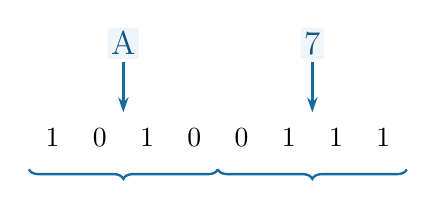
\begin{tikzpicture}[x=1mm,y=1mm]
\node[vc digit] (s0) at (9.0,0) {$ \mathrm{A} $};
\draw[vc arrow] (s0.south)--(9.0,-9);
\node[vc digit] (s1) at (33.0,0) {$ 7 $};
\draw[vc arrow] (s1.south)--(33.0,-9);
\node[vc bit] (raw0) at (0,-12) {$ 1 $};
\node[vc bit] (raw1) at (6,-12) {$ 0 $};
\node[vc bit] (raw2) at (12,-12) {$ 1 $};
\node[vc bit] (raw3) at (18,-12) {$ 0 $};
\node[vc bit] (raw4) at (24,-12) {$ 0 $};
\node[vc bit] (raw5) at (30,-12) {$ 1 $};
\node[vc bit] (raw6) at (36,-12) {$ 1 $};
\node[vc bit] (raw7) at (42,-12) {$ 1 $};
\draw[vc brace] (-3.0,-16)--(21.0,-16);
\draw[vc brace] (21.0,-16)--(45.0,-16);
\end{tikzpicture}\end{chThreeDiagram}
\end{minipage}\par
\[\therefore\ (A7)_{16}=(10100111)_{2}.\]
\end{minipage}\par
\par\noindent\begin{minipage}{\linewidth}
\convExample{২}{শুধু ভগ্নাংশ}
$ (0.6D)_{16} $-কে ২ ভিত্তিতে রূপান্তর করো।\par
\par\noindent\begin{minipage}{\linewidth}\centering
\phantomsection\label{VC053}
\begin{chThreeDiagram}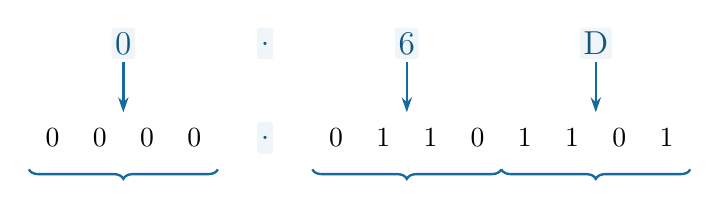
\begin{tikzpicture}[x=1mm,y=1mm]
\node[vc digit] (s0) at (9.0,0) {$ 0 $};
\draw[vc arrow] (s0.south)--(9.0,-9);
\node[vc digit] (s1) at (45.0,0) {$ 6 $};
\draw[vc arrow] (s1.south)--(45.0,-9);
\node[vc digit] (s2) at (69.0,0) {$ \mathrm{D} $};
\draw[vc arrow] (s2.south)--(69.0,-9);
\node[vc digit] at (27.0,0) {$.$};
\node[vc bit] (raw0) at (0,-12) {$ 0 $};
\node[vc bit] (raw1) at (6,-12) {$ 0 $};
\node[vc bit] (raw2) at (12,-12) {$ 0 $};
\node[vc bit] (raw3) at (18,-12) {$ 0 $};
\node[vc bit] (raw4) at (36.0,-12) {$ 0 $};
\node[vc bit] (raw5) at (42.0,-12) {$ 1 $};
\node[vc bit] (raw6) at (48.0,-12) {$ 1 $};
\node[vc bit] (raw7) at (54.0,-12) {$ 0 $};
\node[vc bit] (raw8) at (60.0,-12) {$ 1 $};
\node[vc bit] (raw9) at (66.0,-12) {$ 1 $};
\node[vc bit] (raw10) at (72.0,-12) {$ 0 $};
\node[vc bit] (raw11) at (78.0,-12) {$ 1 $};
\node[vc digit] at (27.0,-12) {$.$};
\draw[vc brace] (-3.0,-16)--(21.0,-16);
\draw[vc brace] (33.0,-16)--(57.0,-16);
\draw[vc brace] (57.0,-16)--(81.0,-16);
\end{tikzpicture}\end{chThreeDiagram}
\end{minipage}\par
\[\therefore\ (0.6D)_{16}=(0.01101101)_{2}.\]
পূর্ণাংশের শুরুর বা ভগ্নাংশের শেষের অপ্রয়োজনীয় ০ বাদ দিয়ে ফল লেখা হয়েছে; ভগ্নাংশের শুরুর ০ বাদ যায় না।\par
\end{minipage}\par
\par\noindent\begin{minipage}{\linewidth}
\convExample{৩}{মিশ্র সংখ্যা}
$ (4D.B8)_{16} $-কে ২ ভিত্তিতে রূপান্তর করো।\par
\par\noindent\begin{minipage}{\linewidth}\centering
\phantomsection\label{VC054}
\begin{chThreeDiagram}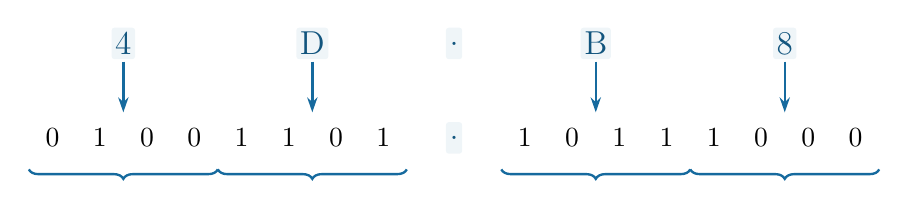
\begin{tikzpicture}[x=1mm,y=1mm]
\node[vc digit] (s0) at (9.0,0) {$ 4 $};
\draw[vc arrow] (s0.south)--(9.0,-9);
\node[vc digit] (s1) at (33.0,0) {$ \mathrm{D} $};
\draw[vc arrow] (s1.south)--(33.0,-9);
\node[vc digit] (s2) at (69.0,0) {$ \mathrm{B} $};
\draw[vc arrow] (s2.south)--(69.0,-9);
\node[vc digit] (s3) at (93.0,0) {$ 8 $};
\draw[vc arrow] (s3.south)--(93.0,-9);
\node[vc digit] at (51.0,0) {$.$};
\node[vc bit] (raw0) at (0,-12) {$ 0 $};
\node[vc bit] (raw1) at (6,-12) {$ 1 $};
\node[vc bit] (raw2) at (12,-12) {$ 0 $};
\node[vc bit] (raw3) at (18,-12) {$ 0 $};
\node[vc bit] (raw4) at (24,-12) {$ 1 $};
\node[vc bit] (raw5) at (30,-12) {$ 1 $};
\node[vc bit] (raw6) at (36,-12) {$ 0 $};
\node[vc bit] (raw7) at (42,-12) {$ 1 $};
\node[vc bit] (raw8) at (60.0,-12) {$ 1 $};
\node[vc bit] (raw9) at (66.0,-12) {$ 0 $};
\node[vc bit] (raw10) at (72.0,-12) {$ 1 $};
\node[vc bit] (raw11) at (78.0,-12) {$ 1 $};
\node[vc bit] (raw12) at (84.0,-12) {$ 1 $};
\node[vc bit] (raw13) at (90.0,-12) {$ 0 $};
\node[vc bit] (raw14) at (96.0,-12) {$ 0 $};
\node[vc bit] (raw15) at (102.0,-12) {$ 0 $};
\node[vc digit] at (51.0,-12) {$.$};
\draw[vc brace] (-3.0,-16)--(21.0,-16);
\draw[vc brace] (21.0,-16)--(45.0,-16);
\draw[vc brace] (57.0,-16)--(81.0,-16);
\draw[vc brace] (81.0,-16)--(105.0,-16);
\end{tikzpicture}\end{chThreeDiagram}
\end{minipage}\par
\[\therefore\ (4D.B8)_{16}=(1001101.10111)_{2}.\]
পূর্ণাংশের শুরুর বা ভগ্নাংশের শেষের অপ্রয়োজনীয় ০ বাদ দিয়ে ফল লেখা হয়েছে; ভগ্নাংশের শুরুর ০ বাদ যায় না।\par
\end{minipage}\par

\subsection{বাইনারি থেকে হেক্সাডেসিমাল}
বিন্দুর দুই পাশ আলাদা করে ৪ বিটের গ্রুপ করো। প্রয়োজনের শূন্য পূর্ণাংশের বামে ও ভগ্নাংশের ডানে বসে।
\par\noindent\begin{minipage}{\linewidth}
\convExample{১}{পূর্ণসংখ্যা}
$ (10101101)_{2} $-কে ১৬ ভিত্তিতে রূপান্তর করো।\par
\par\noindent\begin{minipage}{\linewidth}\centering
\phantomsection\label{VC023}
\begin{chThreeDiagram}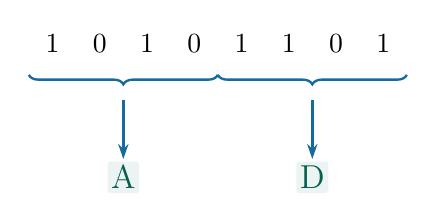
\begin{tikzpicture}[x=1mm,y=1mm]
\node[vc bit] (raw0) at (0,0) {$ 1 $};
\node[vc bit] (raw1) at (6,0) {$ 0 $};
\node[vc bit] (raw2) at (12,0) {$ 1 $};
\node[vc bit] (raw3) at (18,0) {$ 0 $};
\node[vc bit] (raw4) at (24,0) {$ 1 $};
\node[vc bit] (raw5) at (30,0) {$ 1 $};
\node[vc bit] (raw6) at (36,0) {$ 0 $};
\node[vc bit] (raw7) at (42,0) {$ 1 $};
\draw[vc brace] (-3.0,-4)--(21.0,-4);
\node[vc result] (g0) at (9.0,-17) {$ \mathrm{A} $};
\draw[vc arrow] (9.0,-7)--(g0.north);
\draw[vc brace] (21.0,-4)--(45.0,-4);
\node[vc result] (g1) at (33.0,-17) {$ \mathrm{D} $};
\draw[vc arrow] (33.0,-7)--(g1.north);
\end{tikzpicture}\end{chThreeDiagram}
\end{minipage}\par
\[\therefore\ (10101101)_{2}=(AD)_{16}.\]
\end{minipage}\par
\par\noindent\begin{minipage}{\linewidth}
\convExample{২}{শুধু ভগ্নাংশ}
$ (0.10111)_{2} $-কে ১৬ ভিত্তিতে রূপান্তর করো।\par
\par\noindent\begin{minipage}{\linewidth}\centering
\phantomsection\label{VC024}
\begin{chThreeDiagram}\begin{tikzpicture}[x=1mm,y=1mm]
\node[vc digit] at (27.0,0) {$.$};
\node[vc bit] (raw0) at (18,0) {$ 0 $};
\node[vc bit] (raw1) at (36.0,0) {$ 1 $};
\node[vc bit] (raw2) at (42.0,0) {$ 0 $};
\node[vc bit] (raw3) at (48.0,0) {$ 1 $};
\node[vc bit] (raw4) at (54.0,0) {$ 1 $};
\node[vc bit] (raw5) at (60.0,0) {$ 1 $};
\node[vc bit] (new0) at (0,-20) {$ 0 $};
\node[vc bit] (new1) at (6,-20) {$ 0 $};
\node[vc bit] (new2) at (12,-20) {$ 0 $};
\node[vc bit] (new3) at (18,-20) {$ 0 $};
\node[vc bit] (new4) at (36.0,-20) {$ 1 $};
\node[vc bit] (new5) at (42.0,-20) {$ 0 $};
\node[vc bit] (new6) at (48.0,-20) {$ 1 $};
\node[vc bit] (new7) at (54.0,-20) {$ 1 $};
\node[vc bit] (new8) at (60.0,-20) {$ 1 $};
\node[vc bit] (new9) at (66.0,-20) {$ 0 $};
\node[vc bit] (new10) at (72.0,-20) {$ 0 $};
\node[vc bit] (new11) at (78.0,-20) {$ 0 $};
\draw[vc arrow,draw=vcBlue!65] (raw0.south)--(18,-17);
\draw[vc arrow,draw=vcBlue!65] (raw1.south)--(36.0,-17);
\draw[vc arrow,draw=vcBlue!65] (raw2.south)--(42.0,-17);
\draw[vc arrow,draw=vcBlue!65] (raw3.south)--(48.0,-17);
\draw[vc arrow,draw=vcBlue!65] (raw4.south)--(54.0,-17);
\draw[vc arrow,draw=vcBlue!65] (raw5.south)--(60.0,-17);
\node[vc digit] at (27.0,-20) {$.$};
\draw[dashed,draw=vcPad,line width=.85pt] (-2.5,-22.8) rectangle (14.5,-17.2);
\node[vcnote,text=vcPad,fill=vcPad!8,inner sep=1.5pt] (pad-left) at (-13.5,-9) {বামে ৩টি ০};
\draw[vc arrow,draw=vcPad] (pad-left.south)--(6.0,-17);
\draw[dashed,draw=vcPad,line width=.85pt] (63.5,-22.8) rectangle (80.5,-17.2);
\node[vcnote,text=vcPad,fill=vcPad!8,inner sep=1.5pt] (pad-right) at (91.5,-9) {ডানে ৩টি ০};
\draw[vc arrow,draw=vcPad] (pad-right.south)--(72.0,-17);
\draw[vc brace] (-3.0,-24)--(21.0,-24);
\node[vc result] (g0) at (9.0,-37) {$ 0 $};
\draw[vc arrow] (9.0,-27)--(g0.north);
\draw[vc brace] (33.0,-24)--(57.0,-24);
\node[vc result] (g1) at (45.0,-37) {$ \mathrm{B} $};
\draw[vc arrow] (45.0,-27)--(g1.north);
\draw[vc brace] (57.0,-24)--(81.0,-24);
\node[vc result] (g2) at (69.0,-37) {$ 8 $};
\draw[vc arrow] (69.0,-27)--(g2.north);
\node[vc digit] at (27.0,-37) {$.$};
\end{tikzpicture}\end{chThreeDiagram}
\end{minipage}\par
\[\therefore\ (0.10111)_{2}=(0.B8)_{16}.\]
দাগঘেরা বিটগুলো গ্রুপ পূরণের জন্য যোগ করা শূন্য; এগুলো মান বদলায়নি।\par
\end{minipage}\par
\par\noindent\begin{minipage}{\linewidth}
\convExample{৩}{মিশ্র সংখ্যা}
$ (1101101.101)_{2} $-কে ১৬ ভিত্তিতে রূপান্তর করো।\par
\par\noindent\begin{minipage}{\linewidth}\centering
\phantomsection\label{VC025}
\begin{chThreeDiagram}\begin{tikzpicture}[x=1mm,y=1mm]
\node[vc digit] at (51.0,0) {$.$};
\node[vc bit] (raw0) at (6,0) {$ 1 $};
\node[vc bit] (raw1) at (12,0) {$ 1 $};
\node[vc bit] (raw2) at (18,0) {$ 0 $};
\node[vc bit] (raw3) at (24,0) {$ 1 $};
\node[vc bit] (raw4) at (30,0) {$ 1 $};
\node[vc bit] (raw5) at (36,0) {$ 0 $};
\node[vc bit] (raw6) at (42,0) {$ 1 $};
\node[vc bit] (raw7) at (60.0,0) {$ 1 $};
\node[vc bit] (raw8) at (66.0,0) {$ 0 $};
\node[vc bit] (raw9) at (72.0,0) {$ 1 $};
\node[vc bit] (new0) at (0,-20) {$ 0 $};
\node[vc bit] (new1) at (6,-20) {$ 1 $};
\node[vc bit] (new2) at (12,-20) {$ 1 $};
\node[vc bit] (new3) at (18,-20) {$ 0 $};
\node[vc bit] (new4) at (24,-20) {$ 1 $};
\node[vc bit] (new5) at (30,-20) {$ 1 $};
\node[vc bit] (new6) at (36,-20) {$ 0 $};
\node[vc bit] (new7) at (42,-20) {$ 1 $};
\node[vc bit] (new8) at (60.0,-20) {$ 1 $};
\node[vc bit] (new9) at (66.0,-20) {$ 0 $};
\node[vc bit] (new10) at (72.0,-20) {$ 1 $};
\node[vc bit] (new11) at (78.0,-20) {$ 0 $};
\draw[vc arrow,draw=vcBlue!65] (raw0.south)--(6,-17);
\draw[vc arrow,draw=vcBlue!65] (raw1.south)--(12,-17);
\draw[vc arrow,draw=vcBlue!65] (raw2.south)--(18,-17);
\draw[vc arrow,draw=vcBlue!65] (raw3.south)--(24,-17);
\draw[vc arrow,draw=vcBlue!65] (raw4.south)--(30,-17);
\draw[vc arrow,draw=vcBlue!65] (raw5.south)--(36,-17);
\draw[vc arrow,draw=vcBlue!65] (raw6.south)--(42,-17);
\draw[vc arrow,draw=vcBlue!65] (raw7.south)--(60.0,-17);
\draw[vc arrow,draw=vcBlue!65] (raw8.south)--(66.0,-17);
\draw[vc arrow,draw=vcBlue!65] (raw9.south)--(72.0,-17);
\node[vc digit] at (51.0,-20) {$.$};
\draw[dashed,draw=vcPad,line width=.85pt] (-2.5,-22.8) rectangle (2.5,-17.2);
\node[vcnote,text=vcPad,fill=vcPad!8,inner sep=1.5pt] (pad-left) at (-13.5,-9) {বামে ১টি ০};
\draw[vc arrow,draw=vcPad] (pad-left.south)--(0.0,-17);
\draw[dashed,draw=vcPad,line width=.85pt] (75.5,-22.8) rectangle (80.5,-17.2);
\node[vcnote,text=vcPad,fill=vcPad!8,inner sep=1.5pt] (pad-right) at (91.5,-9) {ডানে ১টি ০};
\draw[vc arrow,draw=vcPad] (pad-right.south)--(78.0,-17);
\draw[vc brace] (-3.0,-24)--(21.0,-24);
\node[vc result] (g0) at (9.0,-37) {$ 6 $};
\draw[vc arrow] (9.0,-27)--(g0.north);
\draw[vc brace] (21.0,-24)--(45.0,-24);
\node[vc result] (g1) at (33.0,-37) {$ \mathrm{D} $};
\draw[vc arrow] (33.0,-27)--(g1.north);
\draw[vc brace] (57.0,-24)--(81.0,-24);
\node[vc result] (g2) at (69.0,-37) {$ \mathrm{A} $};
\draw[vc arrow] (69.0,-27)--(g2.north);
\node[vc digit] at (51.0,-37) {$.$};
\end{tikzpicture}\end{chThreeDiagram}
\end{minipage}\par
\[\therefore\ (1101101.101)_{2}=(6D.A)_{16}.\]
দাগঘেরা বিটগুলো গ্রুপ পূরণের জন্য যোগ করা শূন্য; এগুলো মান বদলায়নি।\par
\end{minipage}\par


\smallhead{অক্টাল ও হেক্সাডেসিমালের পারস্পরিক রূপান্তর}
\subsection{অক্টাল থেকে হেক্সাডেসিমাল}
প্রতি অক্টাল অঙ্কে ৩ বিট, প্রতি হেক্সাডেসিমাল অঙ্কে ৪ বিট। বিন্দুর দুই পাশ আলাদা করে ৪ বিটের গ্রুপ করো। প্রয়োজনের শূন্য পূর্ণাংশের বামে ও ভগ্নাংশের ডানে বসে।
\par\noindent\begin{minipage}{\linewidth}
\convExample{১}{পূর্ণসংখ্যা}
$ (527)_{8} $-কে ১৬ ভিত্তিতে রূপান্তর করো।\par
\par\noindent\begin{minipage}{\linewidth}\centering
\phantomsection\label{VC039}
\begin{chThreeDiagram}\begin{tikzpicture}[x=1mm,y=1mm]
\node[vc digit] (s0) at (24.0,0) {$ 5 $};
\draw[vc arrow] (s0.south)--(24.0,-9);
\node[vc digit] (s1) at (42.0,0) {$ 2 $};
\draw[vc arrow] (s1.south)--(42.0,-9);
\node[vc digit] (s2) at (60.0,0) {$ 7 $};
\draw[vc arrow] (s2.south)--(60.0,-9);
\node[vc bit] (raw0) at (18,-12) {$ 1 $};
\node[vc bit] (raw1) at (24,-12) {$ 0 $};
\node[vc bit] (raw2) at (30,-12) {$ 1 $};
\node[vc bit] (raw3) at (36,-12) {$ 0 $};
\node[vc bit] (raw4) at (42,-12) {$ 1 $};
\node[vc bit] (raw5) at (48,-12) {$ 0 $};
\node[vc bit] (raw6) at (54,-12) {$ 1 $};
\node[vc bit] (raw7) at (60,-12) {$ 1 $};
\node[vc bit] (raw8) at (66,-12) {$ 1 $};
\draw[vc brace] (15.0,-16)--(33.0,-16);
\draw[vc brace] (33.0,-16)--(51.0,-16);
\draw[vc brace] (51.0,-16)--(69.0,-16);
\node[vc bit] (new0) at (0,-32) {$ 0 $};
\node[vc bit] (new1) at (6,-32) {$ 0 $};
\node[vc bit] (new2) at (12,-32) {$ 0 $};
\node[vc bit] (new3) at (18,-32) {$ 1 $};
\node[vc bit] (new4) at (24,-32) {$ 0 $};
\node[vc bit] (new5) at (30,-32) {$ 1 $};
\node[vc bit] (new6) at (36,-32) {$ 0 $};
\node[vc bit] (new7) at (42,-32) {$ 1 $};
\node[vc bit] (new8) at (48,-32) {$ 0 $};
\node[vc bit] (new9) at (54,-32) {$ 1 $};
\node[vc bit] (new10) at (60,-32) {$ 1 $};
\node[vc bit] (new11) at (66,-32) {$ 1 $};
\draw[vc arrow,draw=vcBlue!65] (18,-21)--(18,-29);
\draw[vc arrow,draw=vcBlue!65] (24,-21)--(24,-29);
\draw[vc arrow,draw=vcBlue!65] (30,-21)--(30,-29);
\draw[vc arrow,draw=vcBlue!65] (36,-21)--(36,-29);
\draw[vc arrow,draw=vcBlue!65] (42,-21)--(42,-29);
\draw[vc arrow,draw=vcBlue!65] (48,-21)--(48,-29);
\draw[vc arrow,draw=vcBlue!65] (54,-21)--(54,-29);
\draw[vc arrow,draw=vcBlue!65] (60,-21)--(60,-29);
\draw[vc arrow,draw=vcBlue!65] (66,-21)--(66,-29);
\draw[dashed,draw=vcPad,line width=.85pt] (-2.5,-34.8) rectangle (14.5,-29.2);
\node[vcnote,text=vcPad,fill=vcPad!8,inner sep=1.5pt] (pad-left) at (-13.5,-21) {বামে ৩টি ০};
\draw[vc arrow,draw=vcPad] (pad-left.south)--(6.0,-29);
\draw[vc brace] (-3.0,-36)--(21.0,-36);
\node[vc result] (g0) at (9.0,-49) {$ 1 $};
\draw[vc arrow] (9.0,-39)--(g0.north);
\draw[vc brace] (21.0,-36)--(45.0,-36);
\node[vc result] (g1) at (33.0,-49) {$ 5 $};
\draw[vc arrow] (33.0,-39)--(g1.north);
\draw[vc brace] (45.0,-36)--(69.0,-36);
\node[vc result] (g2) at (57.0,-49) {$ 7 $};
\draw[vc arrow] (57.0,-39)--(g2.north);
\end{tikzpicture}\end{chThreeDiagram}
\end{minipage}\par
\[\therefore\ (527)_{8}=(157)_{16}.\]
দাগঘেরা বিটগুলো গ্রুপ পূরণের জন্য যোগ করা শূন্য; এগুলো মান বদলায়নি।\par
\end{minipage}\par
\par\noindent\begin{minipage}{\linewidth}
\convExample{২}{শুধু ভগ্নাংশ}
$ (0.56)_{8} $-কে ১৬ ভিত্তিতে রূপান্তর করো।\par
\par\noindent\begin{minipage}{\linewidth}\centering
\phantomsection\label{VC040}
\begin{chThreeDiagram}\begin{tikzpicture}[x=1mm,y=1mm]
\node[vc digit] (s0) at (12.0,0) {$ 0 $};
\draw[vc arrow] (s0.south)--(12.0,-9);
\node[vc digit] (s1) at (42.0,0) {$ 5 $};
\draw[vc arrow] (s1.south)--(42.0,-9);
\node[vc digit] (s2) at (60.0,0) {$ 6 $};
\draw[vc arrow] (s2.south)--(60.0,-9);
\node[vc digit] at (27.0,0) {$.$};
\node[vc bit] (raw0) at (6,-12) {$ 0 $};
\node[vc bit] (raw1) at (12,-12) {$ 0 $};
\node[vc bit] (raw2) at (18,-12) {$ 0 $};
\node[vc bit] (raw3) at (36.0,-12) {$ 1 $};
\node[vc bit] (raw4) at (42.0,-12) {$ 0 $};
\node[vc bit] (raw5) at (48.0,-12) {$ 1 $};
\node[vc bit] (raw6) at (54.0,-12) {$ 1 $};
\node[vc bit] (raw7) at (60.0,-12) {$ 1 $};
\node[vc bit] (raw8) at (66.0,-12) {$ 0 $};
\node[vc digit] at (27.0,-12) {$.$};
\draw[vc brace] (3.0,-16)--(21.0,-16);
\draw[vc brace] (33.0,-16)--(51.0,-16);
\draw[vc brace] (51.0,-16)--(69.0,-16);
\node[vc bit] (new0) at (0,-32) {$ 0 $};
\node[vc bit] (new1) at (6,-32) {$ 0 $};
\node[vc bit] (new2) at (12,-32) {$ 0 $};
\node[vc bit] (new3) at (18,-32) {$ 0 $};
\node[vc bit] (new4) at (36.0,-32) {$ 1 $};
\node[vc bit] (new5) at (42.0,-32) {$ 0 $};
\node[vc bit] (new6) at (48.0,-32) {$ 1 $};
\node[vc bit] (new7) at (54.0,-32) {$ 1 $};
\node[vc bit] (new8) at (60.0,-32) {$ 1 $};
\node[vc bit] (new9) at (66.0,-32) {$ 0 $};
\node[vc bit] (new10) at (72.0,-32) {$ 0 $};
\node[vc bit] (new11) at (78.0,-32) {$ 0 $};
\draw[vc arrow,draw=vcBlue!65] (6,-21)--(6,-29);
\draw[vc arrow,draw=vcBlue!65] (12,-21)--(12,-29);
\draw[vc arrow,draw=vcBlue!65] (18,-21)--(18,-29);
\draw[vc arrow,draw=vcBlue!65] (36.0,-21)--(36.0,-29);
\draw[vc arrow,draw=vcBlue!65] (42.0,-21)--(42.0,-29);
\draw[vc arrow,draw=vcBlue!65] (48.0,-21)--(48.0,-29);
\draw[vc arrow,draw=vcBlue!65] (54.0,-21)--(54.0,-29);
\draw[vc arrow,draw=vcBlue!65] (60.0,-21)--(60.0,-29);
\draw[vc arrow,draw=vcBlue!65] (66.0,-21)--(66.0,-29);
\node[vc digit] at (27.0,-32) {$.$};
\draw[dashed,draw=vcPad,line width=.85pt] (-2.5,-34.8) rectangle (2.5,-29.2);
\node[vcnote,text=vcPad,fill=vcPad!8,inner sep=1.5pt] (pad-left) at (-13.5,-21) {বামে ১টি ০};
\draw[vc arrow,draw=vcPad] (pad-left.south)--(0.0,-29);
\draw[dashed,draw=vcPad,line width=.85pt] (69.5,-34.8) rectangle (80.5,-29.2);
\node[vcnote,text=vcPad,fill=vcPad!8,inner sep=1.5pt] (pad-right) at (91.5,-21) {ডানে ২টি ০};
\draw[vc arrow,draw=vcPad] (pad-right.south)--(75.0,-29);
\draw[vc brace] (-3.0,-36)--(21.0,-36);
\node[vc result] (g0) at (9.0,-49) {$ 0 $};
\draw[vc arrow] (9.0,-39)--(g0.north);
\draw[vc brace] (33.0,-36)--(57.0,-36);
\node[vc result] (g1) at (45.0,-49) {$ \mathrm{B} $};
\draw[vc arrow] (45.0,-39)--(g1.north);
\draw[vc brace] (57.0,-36)--(81.0,-36);
\node[vc result] (g2) at (69.0,-49) {$ 8 $};
\draw[vc arrow] (69.0,-39)--(g2.north);
\node[vc digit] at (27.0,-49) {$.$};
\end{tikzpicture}\end{chThreeDiagram}
\end{minipage}\par
\[\therefore\ (0.56)_{8}=(0.B8)_{16}.\]
দাগঘেরা বিটগুলো গ্রুপ পূরণের জন্য যোগ করা শূন্য; এগুলো মান বদলায়নি।\par
\end{minipage}\par
\par\noindent\begin{minipage}{\linewidth}
\convExample{৩}{মিশ্র সংখ্যা}
$ (264.35)_{8} $-কে ১৬ ভিত্তিতে রূপান্তর করো।\par
\par\noindent\begin{minipage}{\linewidth}\centering
\phantomsection\label{VC041}
\begin{chThreeDiagram}\begin{tikzpicture}[x=1mm,y=1mm]
\node[vc digit] (s0) at (24.0,0) {$ 2 $};
\draw[vc arrow] (s0.south)--(24.0,-9);
\node[vc digit] (s1) at (42.0,0) {$ 6 $};
\draw[vc arrow] (s1.south)--(42.0,-9);
\node[vc digit] (s2) at (60.0,0) {$ 4 $};
\draw[vc arrow] (s2.south)--(60.0,-9);
\node[vc digit] (s3) at (90.0,0) {$ 3 $};
\draw[vc arrow] (s3.south)--(90.0,-9);
\node[vc digit] (s4) at (108.0,0) {$ 5 $};
\draw[vc arrow] (s4.south)--(108.0,-9);
\node[vc digit] at (75.0,0) {$.$};
\node[vc bit] (raw0) at (18,-12) {$ 0 $};
\node[vc bit] (raw1) at (24,-12) {$ 1 $};
\node[vc bit] (raw2) at (30,-12) {$ 0 $};
\node[vc bit] (raw3) at (36,-12) {$ 1 $};
\node[vc bit] (raw4) at (42,-12) {$ 1 $};
\node[vc bit] (raw5) at (48,-12) {$ 0 $};
\node[vc bit] (raw6) at (54,-12) {$ 1 $};
\node[vc bit] (raw7) at (60,-12) {$ 0 $};
\node[vc bit] (raw8) at (66,-12) {$ 0 $};
\node[vc bit] (raw9) at (84.0,-12) {$ 0 $};
\node[vc bit] (raw10) at (90.0,-12) {$ 1 $};
\node[vc bit] (raw11) at (96.0,-12) {$ 1 $};
\node[vc bit] (raw12) at (102.0,-12) {$ 1 $};
\node[vc bit] (raw13) at (108.0,-12) {$ 0 $};
\node[vc bit] (raw14) at (114.0,-12) {$ 1 $};
\node[vc digit] at (75.0,-12) {$.$};
\draw[vc brace] (15.0,-16)--(33.0,-16);
\draw[vc brace] (33.0,-16)--(51.0,-16);
\draw[vc brace] (51.0,-16)--(69.0,-16);
\draw[vc brace] (81.0,-16)--(99.0,-16);
\draw[vc brace] (99.0,-16)--(117.0,-16);
\node[vc bit] (new0) at (0,-32) {$ 0 $};
\node[vc bit] (new1) at (6,-32) {$ 0 $};
\node[vc bit] (new2) at (12,-32) {$ 0 $};
\node[vc bit] (new3) at (18,-32) {$ 0 $};
\node[vc bit] (new4) at (24,-32) {$ 1 $};
\node[vc bit] (new5) at (30,-32) {$ 0 $};
\node[vc bit] (new6) at (36,-32) {$ 1 $};
\node[vc bit] (new7) at (42,-32) {$ 1 $};
\node[vc bit] (new8) at (48,-32) {$ 0 $};
\node[vc bit] (new9) at (54,-32) {$ 1 $};
\node[vc bit] (new10) at (60,-32) {$ 0 $};
\node[vc bit] (new11) at (66,-32) {$ 0 $};
\node[vc bit] (new12) at (84.0,-32) {$ 0 $};
\node[vc bit] (new13) at (90.0,-32) {$ 1 $};
\node[vc bit] (new14) at (96.0,-32) {$ 1 $};
\node[vc bit] (new15) at (102.0,-32) {$ 1 $};
\node[vc bit] (new16) at (108.0,-32) {$ 0 $};
\node[vc bit] (new17) at (114.0,-32) {$ 1 $};
\node[vc bit] (new18) at (120.0,-32) {$ 0 $};
\node[vc bit] (new19) at (126.0,-32) {$ 0 $};
\draw[vc arrow,draw=vcBlue!65] (18,-21)--(18,-29);
\draw[vc arrow,draw=vcBlue!65] (24,-21)--(24,-29);
\draw[vc arrow,draw=vcBlue!65] (30,-21)--(30,-29);
\draw[vc arrow,draw=vcBlue!65] (36,-21)--(36,-29);
\draw[vc arrow,draw=vcBlue!65] (42,-21)--(42,-29);
\draw[vc arrow,draw=vcBlue!65] (48,-21)--(48,-29);
\draw[vc arrow,draw=vcBlue!65] (54,-21)--(54,-29);
\draw[vc arrow,draw=vcBlue!65] (60,-21)--(60,-29);
\draw[vc arrow,draw=vcBlue!65] (66,-21)--(66,-29);
\draw[vc arrow,draw=vcBlue!65] (84.0,-21)--(84.0,-29);
\draw[vc arrow,draw=vcBlue!65] (90.0,-21)--(90.0,-29);
\draw[vc arrow,draw=vcBlue!65] (96.0,-21)--(96.0,-29);
\draw[vc arrow,draw=vcBlue!65] (102.0,-21)--(102.0,-29);
\draw[vc arrow,draw=vcBlue!65] (108.0,-21)--(108.0,-29);
\draw[vc arrow,draw=vcBlue!65] (114.0,-21)--(114.0,-29);
\node[vc digit] at (75.0,-32) {$.$};
\draw[dashed,draw=vcPad,line width=.85pt] (-2.5,-34.8) rectangle (14.5,-29.2);
\node[vcnote,text=vcPad,fill=vcPad!8,inner sep=1.5pt] (pad-left) at (-13.5,-21) {বামে ৩টি ০};
\draw[vc arrow,draw=vcPad] (pad-left.south)--(6.0,-29);
\draw[dashed,draw=vcPad,line width=.85pt] (117.5,-34.8) rectangle (128.5,-29.2);
\node[vcnote,text=vcPad,fill=vcPad!8,inner sep=1.5pt] (pad-right) at (139.5,-21) {ডানে ২টি ০};
\draw[vc arrow,draw=vcPad] (pad-right.south)--(123.0,-29);
\draw[vc brace] (-3.0,-36)--(21.0,-36);
\node[vc result] (g0) at (9.0,-49) {$ 0 $};
\draw[vc arrow] (9.0,-39)--(g0.north);
\draw[vc brace] (21.0,-36)--(45.0,-36);
\node[vc result] (g1) at (33.0,-49) {$ \mathrm{B} $};
\draw[vc arrow] (33.0,-39)--(g1.north);
\draw[vc brace] (45.0,-36)--(69.0,-36);
\node[vc result] (g2) at (57.0,-49) {$ 4 $};
\draw[vc arrow] (57.0,-39)--(g2.north);
\draw[vc brace] (81.0,-36)--(105.0,-36);
\node[vc result] (g3) at (93.0,-49) {$ 7 $};
\draw[vc arrow] (93.0,-39)--(g3.north);
\draw[vc brace] (105.0,-36)--(129.0,-36);
\node[vc result] (g4) at (117.0,-49) {$ 4 $};
\draw[vc arrow] (117.0,-39)--(g4.north);
\node[vc digit] at (75.0,-49) {$.$};
\end{tikzpicture}\end{chThreeDiagram}
\end{minipage}\par
\[\therefore\ (264.35)_{8}=(B4.74)_{16}.\]
দাগঘেরা বিটগুলো গ্রুপ পূরণের জন্য যোগ করা শূন্য; এগুলো মান বদলায়নি।\par
পূর্ণাংশের শুরুর বা ভগ্নাংশের শেষের অপ্রয়োজনীয় ০ বাদ দিয়ে ফল লেখা হয়েছে; ভগ্নাংশের শুরুর ০ বাদ যায় না।\par
\end{minipage}\par

\subsection{হেক্সাডেসিমাল থেকে অক্টাল}
প্রতি অক্টাল অঙ্কে ৩ বিট, প্রতি হেক্সাডেসিমাল অঙ্কে ৪ বিট। বিন্দুর দুই পাশ আলাদা করে ৩ বিটের গ্রুপ করো। প্রয়োজনের শূন্য পূর্ণাংশের বামে ও ভগ্নাংশের ডানে বসে।
\par\noindent\begin{minipage}{\linewidth}
\convExample{১}{পূর্ণসংখ্যা}
$ (2B9)_{16} $-কে ৮ ভিত্তিতে রূপান্তর করো।\par
\par\noindent\begin{minipage}{\linewidth}\centering
\phantomsection\label{VC055}
\begin{chThreeDiagram}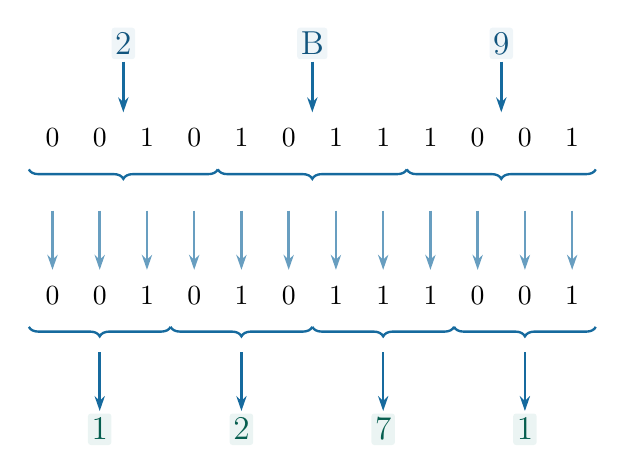
\begin{tikzpicture}[x=1mm,y=1mm]
\node[vc digit] (s0) at (9.0,0) {$ 2 $};
\draw[vc arrow] (s0.south)--(9.0,-9);
\node[vc digit] (s1) at (33.0,0) {$ \mathrm{B} $};
\draw[vc arrow] (s1.south)--(33.0,-9);
\node[vc digit] (s2) at (57.0,0) {$ 9 $};
\draw[vc arrow] (s2.south)--(57.0,-9);
\node[vc bit] (raw0) at (0,-12) {$ 0 $};
\node[vc bit] (raw1) at (6,-12) {$ 0 $};
\node[vc bit] (raw2) at (12,-12) {$ 1 $};
\node[vc bit] (raw3) at (18,-12) {$ 0 $};
\node[vc bit] (raw4) at (24,-12) {$ 1 $};
\node[vc bit] (raw5) at (30,-12) {$ 0 $};
\node[vc bit] (raw6) at (36,-12) {$ 1 $};
\node[vc bit] (raw7) at (42,-12) {$ 1 $};
\node[vc bit] (raw8) at (48,-12) {$ 1 $};
\node[vc bit] (raw9) at (54,-12) {$ 0 $};
\node[vc bit] (raw10) at (60,-12) {$ 0 $};
\node[vc bit] (raw11) at (66,-12) {$ 1 $};
\draw[vc brace] (-3.0,-16)--(21.0,-16);
\draw[vc brace] (21.0,-16)--(45.0,-16);
\draw[vc brace] (45.0,-16)--(69.0,-16);
\node[vc bit] (new0) at (0,-32) {$ 0 $};
\node[vc bit] (new1) at (6,-32) {$ 0 $};
\node[vc bit] (new2) at (12,-32) {$ 1 $};
\node[vc bit] (new3) at (18,-32) {$ 0 $};
\node[vc bit] (new4) at (24,-32) {$ 1 $};
\node[vc bit] (new5) at (30,-32) {$ 0 $};
\node[vc bit] (new6) at (36,-32) {$ 1 $};
\node[vc bit] (new7) at (42,-32) {$ 1 $};
\node[vc bit] (new8) at (48,-32) {$ 1 $};
\node[vc bit] (new9) at (54,-32) {$ 0 $};
\node[vc bit] (new10) at (60,-32) {$ 0 $};
\node[vc bit] (new11) at (66,-32) {$ 1 $};
\draw[vc arrow,draw=vcBlue!65] (0,-21)--(0,-29);
\draw[vc arrow,draw=vcBlue!65] (6,-21)--(6,-29);
\draw[vc arrow,draw=vcBlue!65] (12,-21)--(12,-29);
\draw[vc arrow,draw=vcBlue!65] (18,-21)--(18,-29);
\draw[vc arrow,draw=vcBlue!65] (24,-21)--(24,-29);
\draw[vc arrow,draw=vcBlue!65] (30,-21)--(30,-29);
\draw[vc arrow,draw=vcBlue!65] (36,-21)--(36,-29);
\draw[vc arrow,draw=vcBlue!65] (42,-21)--(42,-29);
\draw[vc arrow,draw=vcBlue!65] (48,-21)--(48,-29);
\draw[vc arrow,draw=vcBlue!65] (54,-21)--(54,-29);
\draw[vc arrow,draw=vcBlue!65] (60,-21)--(60,-29);
\draw[vc arrow,draw=vcBlue!65] (66,-21)--(66,-29);
\draw[vc brace] (-3.0,-36)--(15.0,-36);
\node[vc result] (g0) at (6.0,-49) {$ 1 $};
\draw[vc arrow] (6.0,-39)--(g0.north);
\draw[vc brace] (15.0,-36)--(33.0,-36);
\node[vc result] (g1) at (24.0,-49) {$ 2 $};
\draw[vc arrow] (24.0,-39)--(g1.north);
\draw[vc brace] (33.0,-36)--(51.0,-36);
\node[vc result] (g2) at (42.0,-49) {$ 7 $};
\draw[vc arrow] (42.0,-39)--(g2.north);
\draw[vc brace] (51.0,-36)--(69.0,-36);
\node[vc result] (g3) at (60.0,-49) {$ 1 $};
\draw[vc arrow] (60.0,-39)--(g3.north);
\end{tikzpicture}\end{chThreeDiagram}
\end{minipage}\par
\[\therefore\ (2B9)_{16}=(1271)_{8}.\]
\end{minipage}\par
\par\noindent\begin{minipage}{\linewidth}
\convExample{২}{শুধু ভগ্নাংশ}
$ (0.9A)_{16} $-কে ৮ ভিত্তিতে রূপান্তর করো।\par
\par\noindent\begin{minipage}{\linewidth}\centering
\phantomsection\label{VC056}
\begin{chThreeDiagram}\begin{tikzpicture}[x=1mm,y=1mm]
\node[vc digit] (s0) at (21.0,0) {$ 0 $};
\draw[vc arrow] (s0.south)--(21.0,-9);
\node[vc digit] (s1) at (57.0,0) {$ 9 $};
\draw[vc arrow] (s1.south)--(57.0,-9);
\node[vc digit] (s2) at (81.0,0) {$ \mathrm{A} $};
\draw[vc arrow] (s2.south)--(81.0,-9);
\node[vc digit] at (39.0,0) {$.$};
\node[vc bit] (raw0) at (12,-12) {$ 0 $};
\node[vc bit] (raw1) at (18,-12) {$ 0 $};
\node[vc bit] (raw2) at (24,-12) {$ 0 $};
\node[vc bit] (raw3) at (30,-12) {$ 0 $};
\node[vc bit] (raw4) at (48.0,-12) {$ 1 $};
\node[vc bit] (raw5) at (54.0,-12) {$ 0 $};
\node[vc bit] (raw6) at (60.0,-12) {$ 0 $};
\node[vc bit] (raw7) at (66.0,-12) {$ 1 $};
\node[vc bit] (raw8) at (72.0,-12) {$ 1 $};
\node[vc bit] (raw9) at (78.0,-12) {$ 0 $};
\node[vc bit] (raw10) at (84.0,-12) {$ 1 $};
\node[vc bit] (raw11) at (90.0,-12) {$ 0 $};
\node[vc digit] at (39.0,-12) {$.$};
\draw[vc brace] (9.0,-16)--(33.0,-16);
\draw[vc brace] (45.0,-16)--(69.0,-16);
\draw[vc brace] (69.0,-16)--(93.0,-16);
\node[vc bit] (new0) at (0,-32) {$ 0 $};
\node[vc bit] (new1) at (6,-32) {$ 0 $};
\node[vc bit] (new2) at (12,-32) {$ 0 $};
\node[vc bit] (new3) at (18,-32) {$ 0 $};
\node[vc bit] (new4) at (24,-32) {$ 0 $};
\node[vc bit] (new5) at (30,-32) {$ 0 $};
\node[vc bit] (new6) at (48.0,-32) {$ 1 $};
\node[vc bit] (new7) at (54.0,-32) {$ 0 $};
\node[vc bit] (new8) at (60.0,-32) {$ 0 $};
\node[vc bit] (new9) at (66.0,-32) {$ 1 $};
\node[vc bit] (new10) at (72.0,-32) {$ 1 $};
\node[vc bit] (new11) at (78.0,-32) {$ 0 $};
\node[vc bit] (new12) at (84.0,-32) {$ 1 $};
\node[vc bit] (new13) at (90.0,-32) {$ 0 $};
\node[vc bit] (new14) at (96.0,-32) {$ 0 $};
\draw[vc arrow,draw=vcBlue!65] (12,-21)--(12,-29);
\draw[vc arrow,draw=vcBlue!65] (18,-21)--(18,-29);
\draw[vc arrow,draw=vcBlue!65] (24,-21)--(24,-29);
\draw[vc arrow,draw=vcBlue!65] (30,-21)--(30,-29);
\draw[vc arrow,draw=vcBlue!65] (48.0,-21)--(48.0,-29);
\draw[vc arrow,draw=vcBlue!65] (54.0,-21)--(54.0,-29);
\draw[vc arrow,draw=vcBlue!65] (60.0,-21)--(60.0,-29);
\draw[vc arrow,draw=vcBlue!65] (66.0,-21)--(66.0,-29);
\draw[vc arrow,draw=vcBlue!65] (72.0,-21)--(72.0,-29);
\draw[vc arrow,draw=vcBlue!65] (78.0,-21)--(78.0,-29);
\draw[vc arrow,draw=vcBlue!65] (84.0,-21)--(84.0,-29);
\draw[vc arrow,draw=vcBlue!65] (90.0,-21)--(90.0,-29);
\node[vc digit] at (39.0,-32) {$.$};
\draw[dashed,draw=vcPad,line width=.85pt] (-2.5,-34.8) rectangle (8.5,-29.2);
\node[vcnote,text=vcPad,fill=vcPad!8,inner sep=1.5pt] (pad-left) at (-13.5,-21) {বামে ২টি ০};
\draw[vc arrow,draw=vcPad] (pad-left.south)--(3.0,-29);
\draw[dashed,draw=vcPad,line width=.85pt] (93.5,-34.8) rectangle (98.5,-29.2);
\node[vcnote,text=vcPad,fill=vcPad!8,inner sep=1.5pt] (pad-right) at (109.5,-21) {ডানে ১টি ০};
\draw[vc arrow,draw=vcPad] (pad-right.south)--(96.0,-29);
\draw[vc brace] (-3.0,-36)--(15.0,-36);
\node[vc result] (g0) at (6.0,-49) {$ 0 $};
\draw[vc arrow] (6.0,-39)--(g0.north);
\draw[vc brace] (15.0,-36)--(33.0,-36);
\node[vc result] (g1) at (24.0,-49) {$ 0 $};
\draw[vc arrow] (24.0,-39)--(g1.north);
\draw[vc brace] (45.0,-36)--(63.0,-36);
\node[vc result] (g2) at (54.0,-49) {$ 4 $};
\draw[vc arrow] (54.0,-39)--(g2.north);
\draw[vc brace] (63.0,-36)--(81.0,-36);
\node[vc result] (g3) at (72.0,-49) {$ 6 $};
\draw[vc arrow] (72.0,-39)--(g3.north);
\draw[vc brace] (81.0,-36)--(99.0,-36);
\node[vc result] (g4) at (90.0,-49) {$ 4 $};
\draw[vc arrow] (90.0,-39)--(g4.north);
\node[vc digit] at (39.0,-49) {$.$};
\end{tikzpicture}\end{chThreeDiagram}
\end{minipage}\par
\[\therefore\ (0.9A)_{16}=(0.464)_{8}.\]
দাগঘেরা বিটগুলো গ্রুপ পূরণের জন্য যোগ করা শূন্য; এগুলো মান বদলায়নি।\par
পূর্ণাংশের শুরুর বা ভগ্নাংশের শেষের অপ্রয়োজনীয় ০ বাদ দিয়ে ফল লেখা হয়েছে; ভগ্নাংশের শুরুর ০ বাদ যায় না।\par
\end{minipage}\par
\par\noindent\begin{minipage}{\linewidth}
\convExample{৩}{মিশ্র সংখ্যা}
$ (6B.92)_{16} $-কে ৮ ভিত্তিতে রূপান্তর করো।\par
\par\noindent\begin{minipage}{\linewidth}\centering
\phantomsection\label{VC057}
\begin{chThreeDiagram}\begin{tikzpicture}[x=1mm,y=1mm]
\node[vc digit] (s0) at (15.0,0) {$ 6 $};
\draw[vc arrow] (s0.south)--(15.0,-9);
\node[vc digit] (s1) at (39.0,0) {$ \mathrm{B} $};
\draw[vc arrow] (s1.south)--(39.0,-9);
\node[vc digit] (s2) at (75.0,0) {$ 9 $};
\draw[vc arrow] (s2.south)--(75.0,-9);
\node[vc digit] (s3) at (99.0,0) {$ 2 $};
\draw[vc arrow] (s3.south)--(99.0,-9);
\node[vc digit] at (57.0,0) {$.$};
\node[vc bit] (raw0) at (6,-12) {$ 0 $};
\node[vc bit] (raw1) at (12,-12) {$ 1 $};
\node[vc bit] (raw2) at (18,-12) {$ 1 $};
\node[vc bit] (raw3) at (24,-12) {$ 0 $};
\node[vc bit] (raw4) at (30,-12) {$ 1 $};
\node[vc bit] (raw5) at (36,-12) {$ 0 $};
\node[vc bit] (raw6) at (42,-12) {$ 1 $};
\node[vc bit] (raw7) at (48,-12) {$ 1 $};
\node[vc bit] (raw8) at (66.0,-12) {$ 1 $};
\node[vc bit] (raw9) at (72.0,-12) {$ 0 $};
\node[vc bit] (raw10) at (78.0,-12) {$ 0 $};
\node[vc bit] (raw11) at (84.0,-12) {$ 1 $};
\node[vc bit] (raw12) at (90.0,-12) {$ 0 $};
\node[vc bit] (raw13) at (96.0,-12) {$ 0 $};
\node[vc bit] (raw14) at (102.0,-12) {$ 1 $};
\node[vc bit] (raw15) at (108.0,-12) {$ 0 $};
\node[vc digit] at (57.0,-12) {$.$};
\draw[vc brace] (3.0,-16)--(27.0,-16);
\draw[vc brace] (27.0,-16)--(51.0,-16);
\draw[vc brace] (63.0,-16)--(87.0,-16);
\draw[vc brace] (87.0,-16)--(111.0,-16);
\node[vc bit] (new0) at (0,-32) {$ 0 $};
\node[vc bit] (new1) at (6,-32) {$ 0 $};
\node[vc bit] (new2) at (12,-32) {$ 1 $};
\node[vc bit] (new3) at (18,-32) {$ 1 $};
\node[vc bit] (new4) at (24,-32) {$ 0 $};
\node[vc bit] (new5) at (30,-32) {$ 1 $};
\node[vc bit] (new6) at (36,-32) {$ 0 $};
\node[vc bit] (new7) at (42,-32) {$ 1 $};
\node[vc bit] (new8) at (48,-32) {$ 1 $};
\node[vc bit] (new9) at (66.0,-32) {$ 1 $};
\node[vc bit] (new10) at (72.0,-32) {$ 0 $};
\node[vc bit] (new11) at (78.0,-32) {$ 0 $};
\node[vc bit] (new12) at (84.0,-32) {$ 1 $};
\node[vc bit] (new13) at (90.0,-32) {$ 0 $};
\node[vc bit] (new14) at (96.0,-32) {$ 0 $};
\node[vc bit] (new15) at (102.0,-32) {$ 1 $};
\node[vc bit] (new16) at (108.0,-32) {$ 0 $};
\node[vc bit] (new17) at (114.0,-32) {$ 0 $};
\draw[vc arrow,draw=vcBlue!65] (6,-21)--(6,-29);
\draw[vc arrow,draw=vcBlue!65] (12,-21)--(12,-29);
\draw[vc arrow,draw=vcBlue!65] (18,-21)--(18,-29);
\draw[vc arrow,draw=vcBlue!65] (24,-21)--(24,-29);
\draw[vc arrow,draw=vcBlue!65] (30,-21)--(30,-29);
\draw[vc arrow,draw=vcBlue!65] (36,-21)--(36,-29);
\draw[vc arrow,draw=vcBlue!65] (42,-21)--(42,-29);
\draw[vc arrow,draw=vcBlue!65] (48,-21)--(48,-29);
\draw[vc arrow,draw=vcBlue!65] (66.0,-21)--(66.0,-29);
\draw[vc arrow,draw=vcBlue!65] (72.0,-21)--(72.0,-29);
\draw[vc arrow,draw=vcBlue!65] (78.0,-21)--(78.0,-29);
\draw[vc arrow,draw=vcBlue!65] (84.0,-21)--(84.0,-29);
\draw[vc arrow,draw=vcBlue!65] (90.0,-21)--(90.0,-29);
\draw[vc arrow,draw=vcBlue!65] (96.0,-21)--(96.0,-29);
\draw[vc arrow,draw=vcBlue!65] (102.0,-21)--(102.0,-29);
\draw[vc arrow,draw=vcBlue!65] (108.0,-21)--(108.0,-29);
\node[vc digit] at (57.0,-32) {$.$};
\draw[dashed,draw=vcPad,line width=.85pt] (-2.5,-34.8) rectangle (2.5,-29.2);
\node[vcnote,text=vcPad,fill=vcPad!8,inner sep=1.5pt] (pad-left) at (-13.5,-21) {বামে ১টি ০};
\draw[vc arrow,draw=vcPad] (pad-left.south)--(0.0,-29);
\draw[dashed,draw=vcPad,line width=.85pt] (111.5,-34.8) rectangle (116.5,-29.2);
\node[vcnote,text=vcPad,fill=vcPad!8,inner sep=1.5pt] (pad-right) at (127.5,-21) {ডানে ১টি ০};
\draw[vc arrow,draw=vcPad] (pad-right.south)--(114.0,-29);
\draw[vc brace] (-3.0,-36)--(15.0,-36);
\node[vc result] (g0) at (6.0,-49) {$ 1 $};
\draw[vc arrow] (6.0,-39)--(g0.north);
\draw[vc brace] (15.0,-36)--(33.0,-36);
\node[vc result] (g1) at (24.0,-49) {$ 5 $};
\draw[vc arrow] (24.0,-39)--(g1.north);
\draw[vc brace] (33.0,-36)--(51.0,-36);
\node[vc result] (g2) at (42.0,-49) {$ 3 $};
\draw[vc arrow] (42.0,-39)--(g2.north);
\draw[vc brace] (63.0,-36)--(81.0,-36);
\node[vc result] (g3) at (72.0,-49) {$ 4 $};
\draw[vc arrow] (72.0,-39)--(g3.north);
\draw[vc brace] (81.0,-36)--(99.0,-36);
\node[vc result] (g4) at (90.0,-49) {$ 4 $};
\draw[vc arrow] (90.0,-39)--(g4.north);
\draw[vc brace] (99.0,-36)--(117.0,-36);
\node[vc result] (g5) at (108.0,-49) {$ 4 $};
\draw[vc arrow] (108.0,-39)--(g5.north);
\node[vc digit] at (57.0,-49) {$.$};
\end{tikzpicture}\end{chThreeDiagram}
\end{minipage}\par
\[\therefore\ (6B.92)_{16}=(153.444)_{8}.\]
দাগঘেরা বিটগুলো গ্রুপ পূরণের জন্য যোগ করা শূন্য; এগুলো মান বদলায়নি।\par
\end{minipage}\par


\smallhead{সাধারণ ভিত্তি ও দুই ধাপের রূপান্তর}
\subsection{\texorpdfstring{দশমিক থেকে $n$ ভিত্তি}{দশমিক থেকে n ভিত্তি}}
পূর্ণাংশে লক্ষ্য ভিত্তি দিয়ে ভাগ করো; ভাগশেষ নিচ থেকে ওপরে পড়ো। ভগ্নাংশে একই ভিত্তি দিয়ে গুণ করে পাওয়া অঙ্ক ওপর থেকে নিচে পড়ো।
\par\noindent\begin{minipage}{\linewidth}
\convExample{১}{পূর্ণসংখ্যা}
$ (83)_{10} $-কে ৫ ভিত্তিতে রূপান্তর করো।\par
\par\noindent\begin{minipage}{\linewidth}\centering
\phantomsection\label{VC013}
\begin{chThreeDiagram}\begin{tikzpicture}[x=1mm,y=1mm]
\path[use as bounding box] (-3,9) rectangle (72,-35);
\node[vcnote] at (15,7) {ভাজ্য/ভাগফল};
\node[vcnote] at (44,7) {ভাগশেষ};
\node[vcnum] at (0.0,0) {$ 5 $};
\node[vcnum] at (10.0,0) {$ 83 $};
\draw[vc line] (5.0,3)--(5.0,-3.5)--(50,-3.5);
\node[vcnum] (r0) at (44,-7) {$ 3 $};
\node[vcnum] at (1.5,-7) {$ 5 $};
\node[vcnum] at (11.5,-7) {$ 16 $};
\draw[vc line] (6.5,-4)--(6.5,-10.5)--(50,-10.5);
\node[vcnum] (r1) at (44,-14) {$ 1 $};
\node[vcnum] at (3.0,-14) {$ 5 $};
\node[vcnum] at (13.0,-14) {$ 3 $};
\draw[vc line] (8.0,-11)--(8.0,-17.5)--(50,-17.5);
\node[vcnum] (r2) at (44,-21) {$ 3 $};
\node[vcnum] at (14.5,-21) {$0$};
\node[vcnote] at (61,-3) {LSB};
\node[vcnote] at (61,-26) {MSB};
\draw[vc arrow] (61,-21)--(61,-7);
\node[vcnote] at (31,-33) {নিচ থেকে ওপরে পড়ো};
\end{tikzpicture}\end{chThreeDiagram}
\end{minipage}\par
\[\therefore\ (83)_{10}=(313)_{5}.\]
\end{minipage}\par
\par\noindent\begin{minipage}{\linewidth}
\convExample{২}{শুধু ভগ্নাংশ}
$ (0.84)_{10} $-কে ৫ ভিত্তিতে রূপান্তর করো।\par
\par\noindent\begin{minipage}{\linewidth}\centering
\phantomsection\label{VC014}
\begin{chThreeDiagram}\begin{tikzpicture}[x=1mm,y=1mm]
\path[use as bounding box] (-9,9) rectangle (76,-39);
\node[vcnote] at (14,7) {প্রাপ্ত অঙ্ক};
\node[vcnote] at (45,7) {ভগ্নাংশ};
\node[vcnum] at (45,0) {$ 0.84 $};
\draw[vc line] (26,3)--(26,-27);
\node[vcnum] (m0) at (45,-5) {$\times 5$};
\draw[vc line] (7,-8)--(65,-8);
\node[vcnum] at (14,-12) {$ 4 $};
\node[vcnum] (f0) at (45,-12) {$ 0.2 $};
\node[vcnum] (m1) at (45,-17) {$\times 5$};
\draw[vc line] (7,-20)--(65,-20);
\node[vcnum] at (14,-24) {$ 1 $};
\node[vcnum] (f1) at (45,-24) {$ 0 $};
\draw[vc arrow] (f0.east)--(72,-12)--(72,-17)--(m1.east);
\node[vcnote] at (0,-8) {MSB};
\node[vcnote] at (0,-29) {LSB};
\draw[vc arrow] (0,-12)--(0,-24);
\node[vcnote] at (34,-36) {ওপর থেকে নিচে পড়ো};
\end{tikzpicture}\end{chThreeDiagram}
\end{minipage}\par
\[\therefore\ (0.84)_{10}=(0.41)_{5}.\]
\end{minipage}\par
\par\noindent\begin{minipage}{\linewidth}
\convExample{৩}{মিশ্র সংখ্যা}
$ (129.6)_{10} $-কে ৫ ভিত্তিতে রূপান্তর করো।\par
\begin{minipage}[t]{.48\linewidth}\vspace{0pt}\centering\textbf{পূর্ণাংশ}\par\vspace{1mm}
\par\noindent\begin{minipage}{\linewidth}\centering
\phantomsection\label{VC015}
\begin{chThreeDiagram}\begin{tikzpicture}[x=1mm,y=1mm]
\path[use as bounding box] (-3,9) rectangle (72,-42);
\node[vcnote] at (15,7) {ভাজ্য/ভাগফল};
\node[vcnote] at (44,7) {ভাগশেষ};
\node[vcnum] at (0.0,0) {$ 5 $};
\node[vcnum] at (10.0,0) {$ 129 $};
\draw[vc line] (5.0,3)--(5.0,-3.5)--(50,-3.5);
\node[vcnum] (r0) at (44,-7) {$ 4 $};
\node[vcnum] at (1.5,-7) {$ 5 $};
\node[vcnum] at (11.5,-7) {$ 25 $};
\draw[vc line] (6.5,-4)--(6.5,-10.5)--(50,-10.5);
\node[vcnum] (r1) at (44,-14) {$ 0 $};
\node[vcnum] at (3.0,-14) {$ 5 $};
\node[vcnum] at (13.0,-14) {$ 5 $};
\draw[vc line] (8.0,-11)--(8.0,-17.5)--(50,-17.5);
\node[vcnum] (r2) at (44,-21) {$ 0 $};
\node[vcnum] at (4.5,-21) {$ 5 $};
\node[vcnum] at (14.5,-21) {$ 1 $};
\draw[vc line] (9.5,-18)--(9.5,-24.5)--(50,-24.5);
\node[vcnum] (r3) at (44,-28) {$ 1 $};
\node[vcnum] at (16.0,-28) {$0$};
\node[vcnote] at (61,-3) {LSB};
\node[vcnote] at (61,-33) {MSB};
\draw[vc arrow] (61,-28)--(61,-7);
\node[vcnote] at (31,-40) {নিচ থেকে ওপরে পড়ো};
\end{tikzpicture}\end{chThreeDiagram}
\end{minipage}\par

$ (1004)_{5} $
\end{minipage}\hfill
\begin{minipage}[t]{.48\linewidth}\vspace{0pt}\centering\textbf{ভগ্নাংশ}\par\vspace{1mm}
\par\noindent\begin{minipage}{\linewidth}\centering
\phantomsection\label{VC016}
\begin{chThreeDiagram}\begin{tikzpicture}[x=1mm,y=1mm]
\path[use as bounding box] (-9,9) rectangle (76,-27);
\node[vcnote] at (14,7) {প্রাপ্ত অঙ্ক};
\node[vcnote] at (45,7) {ভগ্নাংশ};
\node[vcnum] at (45,0) {$ 0.6 $};
\draw[vc line] (26,3)--(26,-15);
\node[vcnum] (m0) at (45,-5) {$\times 5$};
\draw[vc line] (7,-8)--(65,-8);
\node[vcnum] at (14,-12) {$ 3 $};
\node[vcnum] (f0) at (45,-12) {$ 0 $};
\node[vcnote] at (0,-10) {MSB=LSB};
\draw[vc arrow] (0,-14)--(0,-20);
\node[vcnote] at (34,-24) {ওপর থেকে নিচে পড়ো};
\end{tikzpicture}\end{chThreeDiagram}
\end{minipage}\par

$ (0.3)_{5} $
\end{minipage}\par
\[\therefore\ (129.6)_{10}=(1004.3)_{5}.\]
\end{minipage}\par

\subsection{\texorpdfstring{বাইনারি থেকে $n$ ভিত্তি}{বাইনারি থেকে n ভিত্তি}}
প্রথমে স্থানমান ব্যবহার করে দশমিকে আনো; তারপর লক্ষ্য ভিত্তিতে ভাগ ও গুণ করো। দুই ধাপের পূর্ণাংশ ও ভগ্নাংশ আলাদাভাবে মিলিয়ে নাও।
\par\noindent\begin{minipage}{\linewidth}
\convExample{১}{পূর্ণসংখ্যা}
$ (11010)_{2} $-কে ৬ ভিত্তিতে রূপান্তর করো।\par
\textbf{প্রথম ধাপ: দশমিক মান}\par
\par\noindent\begin{minipage}{\linewidth}\centering
\phantomsection\label{VC026}
\begin{chThreeDiagram}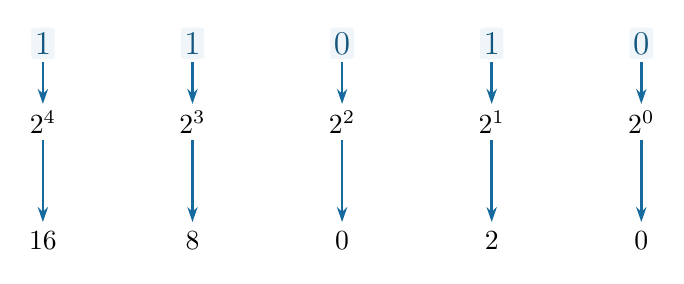
\begin{tikzpicture}[x=1mm,y=1mm]
\node[vc digit] (d0) at (0,0) {$ 1 $};
\node[vcnum] (w0) at (0,-10) {$ 2^{4} $};
\node[vcnum] (v0) at (0,-25) {$ 16 $};
\draw[vc arrow] (d0.south)--(w0.north);
\draw[vc arrow] (w0.south)--(v0.north);
\node[vc digit] (d1) at (19,0) {$ 1 $};
\node[vcnum] (w1) at (19,-10) {$ 2^{3} $};
\node[vcnum] (v1) at (19,-25) {$ 8 $};
\draw[vc arrow] (d1.south)--(w1.north);
\draw[vc arrow] (w1.south)--(v1.north);
\node[vc digit] (d2) at (38,0) {$ 0 $};
\node[vcnum] (w2) at (38,-10) {$ 2^{2} $};
\node[vcnum] (v2) at (38,-25) {$ 0 $};
\draw[vc arrow] (d2.south)--(w2.north);
\draw[vc arrow] (w2.south)--(v2.north);
\node[vc digit] (d3) at (57,0) {$ 1 $};
\node[vcnum] (w3) at (57,-10) {$ 2^{1} $};
\node[vcnum] (v3) at (57,-25) {$ 2 $};
\draw[vc arrow] (d3.south)--(w3.north);
\draw[vc arrow] (w3.south)--(v3.north);
\node[vc digit] (d4) at (76,0) {$ 0 $};
\node[vcnum] (w4) at (76,-10) {$ 2^{0} $};
\node[vcnum] (v4) at (76,-25) {$ 0 $};
\draw[vc arrow] (d4.south)--(w4.north);
\draw[vc arrow] (w4.south)--(v4.north);
\end{tikzpicture}\end{chThreeDiagram}
\end{minipage}\par

\[\begin{aligned}V&=1\times 2^{4}+1\times 2^{3}+0\times 2^{2}+1\times 2^{1}+0\times 2^{0}\\&=16+8+2=26.\end{aligned}\]
\textbf{দ্বিতীয় ধাপ: লক্ষ্য ভিত্তি}\par
\par\noindent\begin{minipage}{\linewidth}\centering
\phantomsection\label{VC027}
\begin{chThreeDiagram}\begin{tikzpicture}[x=1mm,y=1mm]
\path[use as bounding box] (-3,9) rectangle (72,-28);
\node[vcnote] at (15,7) {ভাজ্য/ভাগফল};
\node[vcnote] at (44,7) {ভাগশেষ};
\node[vcnum] at (0.0,0) {$ 6 $};
\node[vcnum] at (10.0,0) {$ 26 $};
\draw[vc line] (5.0,3)--(5.0,-3.5)--(50,-3.5);
\node[vcnum] (r0) at (44,-7) {$ 2 $};
\node[vcnum] at (1.5,-7) {$ 6 $};
\node[vcnum] at (11.5,-7) {$ 4 $};
\draw[vc line] (6.5,-4)--(6.5,-10.5)--(50,-10.5);
\node[vcnum] (r1) at (44,-14) {$ 4 $};
\node[vcnum] at (13.0,-14) {$0$};
\node[vcnote] at (61,-3) {LSB};
\node[vcnote] at (61,-19) {MSB};
\draw[vc arrow] (61,-14)--(61,-7);
\node[vcnote] at (31,-26) {নিচ থেকে ওপরে পড়ো};
\end{tikzpicture}\end{chThreeDiagram}
\end{minipage}\par
\[\therefore\ (11010)_{2}=(42)_{6}.\]
\end{minipage}\par
\par\noindent\begin{minipage}{\linewidth}
\convExample{২}{শুধু ভগ্নাংশ}
$ (0.11)_{2} $-কে ৬ ভিত্তিতে রূপান্তর করো।\par
\textbf{প্রথম ধাপ: দশমিক মান}\par
\par\noindent\begin{minipage}{\linewidth}\centering
\phantomsection\label{VC028}
\begin{chThreeDiagram}\begin{tikzpicture}[x=1mm,y=1mm]
\node[vc digit] (d0) at (0,0) {$ 0 $};
\node[vcnum] (w0) at (0,-10) {$ 2^{0} $};
\node[vcnum] (v0) at (0,-25) {$ 0 $};
\draw[vc arrow] (d0.south)--(w0.north);
\draw[vc arrow] (w0.south)--(v0.north);
\node[vc digit] (d1) at (27,0) {$ 1 $};
\node[vcnum] (w1) at (27,-10) {$ 2^{-1} $};
\node[vcnum] (v1) at (27,-25) {$ \frac{1}{2} $};
\draw[vc arrow] (d1.south)--(w1.north);
\draw[vc arrow] (w1.south)--(v1.north);
\node[vc digit] (d2) at (46,0) {$ 1 $};
\node[vcnum] (w2) at (46,-10) {$ 2^{-2} $};
\node[vcnum] (v2) at (46,-25) {$ \frac{1}{4} $};
\draw[vc arrow] (d2.south)--(w2.north);
\draw[vc arrow] (w2.south)--(v2.north);
\node[vc digit] at (13.5,0) {$.$};
\end{tikzpicture}\end{chThreeDiagram}
\end{minipage}\par

\[\begin{aligned}V&=0\times 2^{0}+1\times 2^{-1}+1\times 2^{-2}\\&=\frac{1}{2}+\frac{1}{4}=0.75.\end{aligned}\]
\textbf{দ্বিতীয় ধাপ: লক্ষ্য ভিত্তি}\par
\par\noindent\begin{minipage}{\linewidth}\centering
\phantomsection\label{VC029}
\begin{chThreeDiagram}\begin{tikzpicture}[x=1mm,y=1mm]
\path[use as bounding box] (-9,9) rectangle (76,-39);
\node[vcnote] at (14,7) {প্রাপ্ত অঙ্ক};
\node[vcnote] at (45,7) {ভগ্নাংশ};
\node[vcnum] at (45,0) {$ 0.75 $};
\draw[vc line] (26,3)--(26,-27);
\node[vcnum] (m0) at (45,-5) {$\times 6$};
\draw[vc line] (7,-8)--(65,-8);
\node[vcnum] at (14,-12) {$ 4 $};
\node[vcnum] (f0) at (45,-12) {$ 0.5 $};
\node[vcnum] (m1) at (45,-17) {$\times 6$};
\draw[vc line] (7,-20)--(65,-20);
\node[vcnum] at (14,-24) {$ 3 $};
\node[vcnum] (f1) at (45,-24) {$ 0 $};
\draw[vc arrow] (f0.east)--(72,-12)--(72,-17)--(m1.east);
\node[vcnote] at (0,-8) {MSB};
\node[vcnote] at (0,-29) {LSB};
\draw[vc arrow] (0,-12)--(0,-24);
\node[vcnote] at (34,-36) {ওপর থেকে নিচে পড়ো};
\end{tikzpicture}\end{chThreeDiagram}
\end{minipage}\par
\[\therefore\ (0.11)_{2}=(0.43)_{6}.\]
\end{minipage}\par
\par\noindent\begin{minipage}{\linewidth}
\convExample{৩}{মিশ্র সংখ্যা}
$ (101101.1)_{2} $-কে ৬ ভিত্তিতে রূপান্তর করো।\par
\textbf{প্রথম ধাপ: দশমিক মান}\par
\par\noindent\begin{minipage}{\linewidth}\centering
\phantomsection\label{VC030}
\begin{chThreeDiagram}\begin{tikzpicture}[x=1mm,y=1mm]
\node[vc digit] (d0) at (0,0) {$ 1 $};
\node[vcnum] (w0) at (0,-10) {$ 2^{5} $};
\node[vcnum] (v0) at (0,-25) {$ 32 $};
\draw[vc arrow] (d0.south)--(w0.north);
\draw[vc arrow] (w0.south)--(v0.north);
\node[vc digit] (d1) at (19,0) {$ 0 $};
\node[vcnum] (w1) at (19,-10) {$ 2^{4} $};
\node[vcnum] (v1) at (19,-25) {$ 0 $};
\draw[vc arrow] (d1.south)--(w1.north);
\draw[vc arrow] (w1.south)--(v1.north);
\node[vc digit] (d2) at (38,0) {$ 1 $};
\node[vcnum] (w2) at (38,-10) {$ 2^{3} $};
\node[vcnum] (v2) at (38,-25) {$ 8 $};
\draw[vc arrow] (d2.south)--(w2.north);
\draw[vc arrow] (w2.south)--(v2.north);
\node[vc digit] (d3) at (57,0) {$ 1 $};
\node[vcnum] (w3) at (57,-10) {$ 2^{2} $};
\node[vcnum] (v3) at (57,-25) {$ 4 $};
\draw[vc arrow] (d3.south)--(w3.north);
\draw[vc arrow] (w3.south)--(v3.north);
\node[vc digit] (d4) at (76,0) {$ 0 $};
\node[vcnum] (w4) at (76,-10) {$ 2^{1} $};
\node[vcnum] (v4) at (76,-25) {$ 0 $};
\draw[vc arrow] (d4.south)--(w4.north);
\draw[vc arrow] (w4.south)--(v4.north);
\node[vc digit] (d5) at (95,0) {$ 1 $};
\node[vcnum] (w5) at (95,-10) {$ 2^{0} $};
\node[vcnum] (v5) at (95,-25) {$ 1 $};
\draw[vc arrow] (d5.south)--(w5.north);
\draw[vc arrow] (w5.south)--(v5.north);
\node[vc digit] (d6) at (122,0) {$ 1 $};
\node[vcnum] (w6) at (122,-10) {$ 2^{-1} $};
\node[vcnum] (v6) at (122,-25) {$ \frac{1}{2} $};
\draw[vc arrow] (d6.south)--(w6.north);
\draw[vc arrow] (w6.south)--(v6.north);
\node[vc digit] at (108.5,0) {$.$};
\end{tikzpicture}\end{chThreeDiagram}
\end{minipage}\par

\[\begin{aligned}V&=1\times 2^{5}+0\times 2^{4}+1\times 2^{3}+1\times 2^{2}+0\times 2^{1}+1\times 2^{0}+1\times 2^{-1}\\&=32+8+4+1+\frac{1}{2}=45.5.\end{aligned}\]
\textbf{দ্বিতীয় ধাপ: লক্ষ্য ভিত্তি}\par
\begin{minipage}[t]{.48\linewidth}\vspace{0pt}\centering\textbf{পূর্ণাংশ}\par\vspace{1mm}
\par\noindent\begin{minipage}{\linewidth}\centering
\phantomsection\label{VC031}
\begin{chThreeDiagram}\begin{tikzpicture}[x=1mm,y=1mm]
\path[use as bounding box] (-3,9) rectangle (72,-35);
\node[vcnote] at (15,7) {ভাজ্য/ভাগফল};
\node[vcnote] at (44,7) {ভাগশেষ};
\node[vcnum] at (0.0,0) {$ 6 $};
\node[vcnum] at (10.0,0) {$ 45 $};
\draw[vc line] (5.0,3)--(5.0,-3.5)--(50,-3.5);
\node[vcnum] (r0) at (44,-7) {$ 3 $};
\node[vcnum] at (1.5,-7) {$ 6 $};
\node[vcnum] at (11.5,-7) {$ 7 $};
\draw[vc line] (6.5,-4)--(6.5,-10.5)--(50,-10.5);
\node[vcnum] (r1) at (44,-14) {$ 1 $};
\node[vcnum] at (3.0,-14) {$ 6 $};
\node[vcnum] at (13.0,-14) {$ 1 $};
\draw[vc line] (8.0,-11)--(8.0,-17.5)--(50,-17.5);
\node[vcnum] (r2) at (44,-21) {$ 1 $};
\node[vcnum] at (14.5,-21) {$0$};
\node[vcnote] at (61,-3) {LSB};
\node[vcnote] at (61,-26) {MSB};
\draw[vc arrow] (61,-21)--(61,-7);
\node[vcnote] at (31,-33) {নিচ থেকে ওপরে পড়ো};
\end{tikzpicture}\end{chThreeDiagram}
\end{minipage}\par

$ (113)_{6} $
\end{minipage}\hfill
\begin{minipage}[t]{.48\linewidth}\vspace{0pt}\centering\textbf{ভগ্নাংশ}\par\vspace{1mm}
\par\noindent\begin{minipage}{\linewidth}\centering
\phantomsection\label{VC032}
\begin{chThreeDiagram}\begin{tikzpicture}[x=1mm,y=1mm]
\path[use as bounding box] (-9,9) rectangle (76,-27);
\node[vcnote] at (14,7) {প্রাপ্ত অঙ্ক};
\node[vcnote] at (45,7) {ভগ্নাংশ};
\node[vcnum] at (45,0) {$ 0.5 $};
\draw[vc line] (26,3)--(26,-15);
\node[vcnum] (m0) at (45,-5) {$\times 6$};
\draw[vc line] (7,-8)--(65,-8);
\node[vcnum] at (14,-12) {$ 3 $};
\node[vcnum] (f0) at (45,-12) {$ 0 $};
\node[vcnote] at (0,-10) {MSB=LSB};
\draw[vc arrow] (0,-14)--(0,-20);
\node[vcnote] at (34,-24) {ওপর থেকে নিচে পড়ো};
\end{tikzpicture}\end{chThreeDiagram}
\end{minipage}\par

$ (0.3)_{6} $
\end{minipage}\par
\[\therefore\ (101101.1)_{2}=(113.3)_{6}.\]
\end{minipage}\par

\subsection{\texorpdfstring{অক্টাল থেকে $n$ ভিত্তি}{অক্টাল থেকে n ভিত্তি}}
প্রথমে স্থানমান ব্যবহার করে দশমিকে আনো; তারপর লক্ষ্য ভিত্তিতে ভাগ ও গুণ করো। দুই ধাপের পূর্ণাংশ ও ভগ্নাংশ আলাদাভাবে মিলিয়ে নাও।
\par\noindent\begin{minipage}{\linewidth}
\convExample{১}{পূর্ণসংখ্যা}
$ (73)_{8} $-কে ৬ ভিত্তিতে রূপান্তর করো।\par
\textbf{প্রথম ধাপ: দশমিক মান}\par
\par\noindent\begin{minipage}{\linewidth}\centering
\phantomsection\label{VC042}
\begin{chThreeDiagram}\begin{tikzpicture}[x=1mm,y=1mm]
\node[vc digit] (d0) at (0,0) {$ 7 $};
\node[vcnum] (w0) at (0,-10) {$ 8^{1} $};
\node[vcnum] (v0) at (0,-25) {$ 56 $};
\draw[vc arrow] (d0.south)--(w0.north);
\draw[vc arrow] (w0.south)--(v0.north);
\node[vc digit] (d1) at (19,0) {$ 3 $};
\node[vcnum] (w1) at (19,-10) {$ 8^{0} $};
\node[vcnum] (v1) at (19,-25) {$ 3 $};
\draw[vc arrow] (d1.south)--(w1.north);
\draw[vc arrow] (w1.south)--(v1.north);
\end{tikzpicture}\end{chThreeDiagram}
\end{minipage}\par

\[\begin{aligned}V&=7\times 8^{1}+3\times 8^{0}\\&=56+3=59.\end{aligned}\]
\textbf{দ্বিতীয় ধাপ: লক্ষ্য ভিত্তি}\par
\par\noindent\begin{minipage}{\linewidth}\centering
\phantomsection\label{VC043}
\begin{chThreeDiagram}\begin{tikzpicture}[x=1mm,y=1mm]
\path[use as bounding box] (-3,9) rectangle (72,-35);
\node[vcnote] at (15,7) {ভাজ্য/ভাগফল};
\node[vcnote] at (44,7) {ভাগশেষ};
\node[vcnum] at (0.0,0) {$ 6 $};
\node[vcnum] at (10.0,0) {$ 59 $};
\draw[vc line] (5.0,3)--(5.0,-3.5)--(50,-3.5);
\node[vcnum] (r0) at (44,-7) {$ 5 $};
\node[vcnum] at (1.5,-7) {$ 6 $};
\node[vcnum] at (11.5,-7) {$ 9 $};
\draw[vc line] (6.5,-4)--(6.5,-10.5)--(50,-10.5);
\node[vcnum] (r1) at (44,-14) {$ 3 $};
\node[vcnum] at (3.0,-14) {$ 6 $};
\node[vcnum] at (13.0,-14) {$ 1 $};
\draw[vc line] (8.0,-11)--(8.0,-17.5)--(50,-17.5);
\node[vcnum] (r2) at (44,-21) {$ 1 $};
\node[vcnum] at (14.5,-21) {$0$};
\node[vcnote] at (61,-3) {LSB};
\node[vcnote] at (61,-26) {MSB};
\draw[vc arrow] (61,-21)--(61,-7);
\node[vcnote] at (31,-33) {নিচ থেকে ওপরে পড়ো};
\end{tikzpicture}\end{chThreeDiagram}
\end{minipage}\par
\[\therefore\ (73)_{8}=(135)_{6}.\]
\end{minipage}\par
\par\noindent\begin{minipage}{\linewidth}
\convExample{২}{শুধু ভগ্নাংশ}
$ (0.4)_{8} $-কে ৬ ভিত্তিতে রূপান্তর করো।\par
\textbf{প্রথম ধাপ: দশমিক মান}\par
\par\noindent\begin{minipage}{\linewidth}\centering
\phantomsection\label{VC044}
\begin{chThreeDiagram}\begin{tikzpicture}[x=1mm,y=1mm]
\node[vc digit] (d0) at (0,0) {$ 0 $};
\node[vcnum] (w0) at (0,-10) {$ 8^{0} $};
\node[vcnum] (v0) at (0,-25) {$ 0 $};
\draw[vc arrow] (d0.south)--(w0.north);
\draw[vc arrow] (w0.south)--(v0.north);
\node[vc digit] (d1) at (27,0) {$ 4 $};
\node[vcnum] (w1) at (27,-10) {$ 8^{-1} $};
\node[vcnum] (v1) at (27,-25) {$ \frac{1}{2} $};
\draw[vc arrow] (d1.south)--(w1.north);
\draw[vc arrow] (w1.south)--(v1.north);
\node[vc digit] at (13.5,0) {$.$};
\end{tikzpicture}\end{chThreeDiagram}
\end{minipage}\par

\[\begin{aligned}V&=0\times 8^{0}+4\times 8^{-1}\\&=\frac{1}{2}=0.5.\end{aligned}\]
\textbf{দ্বিতীয় ধাপ: লক্ষ্য ভিত্তি}\par
\par\noindent\begin{minipage}{\linewidth}\centering
\phantomsection\label{VC045}
\begin{chThreeDiagram}\begin{tikzpicture}[x=1mm,y=1mm]
\path[use as bounding box] (-9,9) rectangle (76,-27);
\node[vcnote] at (14,7) {প্রাপ্ত অঙ্ক};
\node[vcnote] at (45,7) {ভগ্নাংশ};
\node[vcnum] at (45,0) {$ 0.5 $};
\draw[vc line] (26,3)--(26,-15);
\node[vcnum] (m0) at (45,-5) {$\times 6$};
\draw[vc line] (7,-8)--(65,-8);
\node[vcnum] at (14,-12) {$ 3 $};
\node[vcnum] (f0) at (45,-12) {$ 0 $};
\node[vcnote] at (0,-10) {MSB=LSB};
\draw[vc arrow] (0,-14)--(0,-20);
\node[vcnote] at (34,-24) {ওপর থেকে নিচে পড়ো};
\end{tikzpicture}\end{chThreeDiagram}
\end{minipage}\par
\[\therefore\ (0.4)_{8}=(0.3)_{6}.\]
\end{minipage}\par
\par\noindent\begin{minipage}{\linewidth}
\convExample{৩}{মিশ্র সংখ্যা}
$ (125.6)_{8} $-কে ৬ ভিত্তিতে রূপান্তর করো।\par
\textbf{প্রথম ধাপ: দশমিক মান}\par
\par\noindent\begin{minipage}{\linewidth}\centering
\phantomsection\label{VC046}
\begin{chThreeDiagram}\begin{tikzpicture}[x=1mm,y=1mm]
\node[vc digit] (d0) at (0,0) {$ 1 $};
\node[vcnum] (w0) at (0,-10) {$ 8^{2} $};
\node[vcnum] (v0) at (0,-25) {$ 64 $};
\draw[vc arrow] (d0.south)--(w0.north);
\draw[vc arrow] (w0.south)--(v0.north);
\node[vc digit] (d1) at (19,0) {$ 2 $};
\node[vcnum] (w1) at (19,-10) {$ 8^{1} $};
\node[vcnum] (v1) at (19,-25) {$ 16 $};
\draw[vc arrow] (d1.south)--(w1.north);
\draw[vc arrow] (w1.south)--(v1.north);
\node[vc digit] (d2) at (38,0) {$ 5 $};
\node[vcnum] (w2) at (38,-10) {$ 8^{0} $};
\node[vcnum] (v2) at (38,-25) {$ 5 $};
\draw[vc arrow] (d2.south)--(w2.north);
\draw[vc arrow] (w2.south)--(v2.north);
\node[vc digit] (d3) at (65,0) {$ 6 $};
\node[vcnum] (w3) at (65,-10) {$ 8^{-1} $};
\node[vcnum] (v3) at (65,-25) {$ \frac{3}{4} $};
\draw[vc arrow] (d3.south)--(w3.north);
\draw[vc arrow] (w3.south)--(v3.north);
\node[vc digit] at (51.5,0) {$.$};
\end{tikzpicture}\end{chThreeDiagram}
\end{minipage}\par

\[\begin{aligned}V&=1\times 8^{2}+2\times 8^{1}+5\times 8^{0}+6\times 8^{-1}\\&=64+16+5+\frac{3}{4}=85.75.\end{aligned}\]
\textbf{দ্বিতীয় ধাপ: লক্ষ্য ভিত্তি}\par
\begin{minipage}[t]{.48\linewidth}\vspace{0pt}\centering\textbf{পূর্ণাংশ}\par\vspace{1mm}
\par\noindent\begin{minipage}{\linewidth}\centering
\phantomsection\label{VC047}
\begin{chThreeDiagram}\begin{tikzpicture}[x=1mm,y=1mm]
\path[use as bounding box] (-3,9) rectangle (72,-35);
\node[vcnote] at (15,7) {ভাজ্য/ভাগফল};
\node[vcnote] at (44,7) {ভাগশেষ};
\node[vcnum] at (0.0,0) {$ 6 $};
\node[vcnum] at (10.0,0) {$ 85 $};
\draw[vc line] (5.0,3)--(5.0,-3.5)--(50,-3.5);
\node[vcnum] (r0) at (44,-7) {$ 1 $};
\node[vcnum] at (1.5,-7) {$ 6 $};
\node[vcnum] at (11.5,-7) {$ 14 $};
\draw[vc line] (6.5,-4)--(6.5,-10.5)--(50,-10.5);
\node[vcnum] (r1) at (44,-14) {$ 2 $};
\node[vcnum] at (3.0,-14) {$ 6 $};
\node[vcnum] at (13.0,-14) {$ 2 $};
\draw[vc line] (8.0,-11)--(8.0,-17.5)--(50,-17.5);
\node[vcnum] (r2) at (44,-21) {$ 2 $};
\node[vcnum] at (14.5,-21) {$0$};
\node[vcnote] at (61,-3) {LSB};
\node[vcnote] at (61,-26) {MSB};
\draw[vc arrow] (61,-21)--(61,-7);
\node[vcnote] at (31,-33) {নিচ থেকে ওপরে পড়ো};
\end{tikzpicture}\end{chThreeDiagram}
\end{minipage}\par

$ (221)_{6} $
\end{minipage}\hfill
\begin{minipage}[t]{.48\linewidth}\vspace{0pt}\centering\textbf{ভগ্নাংশ}\par\vspace{1mm}
\par\noindent\begin{minipage}{\linewidth}\centering
\phantomsection\label{VC048}
\begin{chThreeDiagram}\begin{tikzpicture}[x=1mm,y=1mm]
\path[use as bounding box] (-9,9) rectangle (76,-39);
\node[vcnote] at (14,7) {প্রাপ্ত অঙ্ক};
\node[vcnote] at (45,7) {ভগ্নাংশ};
\node[vcnum] at (45,0) {$ 0.75 $};
\draw[vc line] (26,3)--(26,-27);
\node[vcnum] (m0) at (45,-5) {$\times 6$};
\draw[vc line] (7,-8)--(65,-8);
\node[vcnum] at (14,-12) {$ 4 $};
\node[vcnum] (f0) at (45,-12) {$ 0.5 $};
\node[vcnum] (m1) at (45,-17) {$\times 6$};
\draw[vc line] (7,-20)--(65,-20);
\node[vcnum] at (14,-24) {$ 3 $};
\node[vcnum] (f1) at (45,-24) {$ 0 $};
\draw[vc arrow] (f0.east)--(72,-12)--(72,-17)--(m1.east);
\node[vcnote] at (0,-8) {MSB};
\node[vcnote] at (0,-29) {LSB};
\draw[vc arrow] (0,-12)--(0,-24);
\node[vcnote] at (34,-36) {ওপর থেকে নিচে পড়ো};
\end{tikzpicture}\end{chThreeDiagram}
\end{minipage}\par

$ (0.43)_{6} $
\end{minipage}\par
\[\therefore\ (125.6)_{8}=(221.43)_{6}.\]
\end{minipage}\par

\subsection{\texorpdfstring{হেক্সাডেসিমাল থেকে $n$ ভিত্তি}{হেক্সাডেসিমাল থেকে n ভিত্তি}}
প্রথমে স্থানমান ব্যবহার করে দশমিকে আনো; তারপর লক্ষ্য ভিত্তিতে ভাগ ও গুণ করো। দুই ধাপের পূর্ণাংশ ও ভগ্নাংশ আলাদাভাবে মিলিয়ে নাও।
\par\noindent\begin{minipage}{\linewidth}
\convExample{১}{পূর্ণসংখ্যা}
$ (D3)_{16} $-কে ৪ ভিত্তিতে রূপান্তর করো।\par
\textbf{প্রথম ধাপ: দশমিক মান}\par
\par\noindent\begin{minipage}{\linewidth}\centering
\phantomsection\label{VC058}
\begin{chThreeDiagram}\begin{tikzpicture}[x=1mm,y=1mm]
\node[vc digit] (d0) at (0,0) {$ \mathrm{D} $};
\node[vcnum] (w0) at (0,-10) {$ 16^{1} $};
\node[vcnum] (v0) at (0,-25) {$ 208 $};
\draw[vc arrow] (d0.south)--(w0.north);
\draw[vc arrow] (w0.south)--(v0.north);
\node[vc digit] (d1) at (19,0) {$ 3 $};
\node[vcnum] (w1) at (19,-10) {$ 16^{0} $};
\node[vcnum] (v1) at (19,-25) {$ 3 $};
\draw[vc arrow] (d1.south)--(w1.north);
\draw[vc arrow] (w1.south)--(v1.north);
\end{tikzpicture}\end{chThreeDiagram}
\end{minipage}\par

\[\begin{aligned}V&=\mathrm{D}\times 16^{1}+3\times 16^{0}\\&=208+3=211.\end{aligned}\]
\textbf{দ্বিতীয় ধাপ: লক্ষ্য ভিত্তি}\par
\par\noindent\begin{minipage}{\linewidth}\centering
\phantomsection\label{VC059}
\begin{chThreeDiagram}\begin{tikzpicture}[x=1mm,y=1mm]
\path[use as bounding box] (-3,9) rectangle (72,-42);
\node[vcnote] at (15,7) {ভাজ্য/ভাগফল};
\node[vcnote] at (44,7) {ভাগশেষ};
\node[vcnum] at (0.0,0) {$ 4 $};
\node[vcnum] at (10.0,0) {$ 211 $};
\draw[vc line] (5.0,3)--(5.0,-3.5)--(50,-3.5);
\node[vcnum] (r0) at (44,-7) {$ 3 $};
\node[vcnum] at (1.5,-7) {$ 4 $};
\node[vcnum] at (11.5,-7) {$ 52 $};
\draw[vc line] (6.5,-4)--(6.5,-10.5)--(50,-10.5);
\node[vcnum] (r1) at (44,-14) {$ 0 $};
\node[vcnum] at (3.0,-14) {$ 4 $};
\node[vcnum] at (13.0,-14) {$ 13 $};
\draw[vc line] (8.0,-11)--(8.0,-17.5)--(50,-17.5);
\node[vcnum] (r2) at (44,-21) {$ 1 $};
\node[vcnum] at (4.5,-21) {$ 4 $};
\node[vcnum] at (14.5,-21) {$ 3 $};
\draw[vc line] (9.5,-18)--(9.5,-24.5)--(50,-24.5);
\node[vcnum] (r3) at (44,-28) {$ 3 $};
\node[vcnum] at (16.0,-28) {$0$};
\node[vcnote] at (61,-3) {LSB};
\node[vcnote] at (61,-33) {MSB};
\draw[vc arrow] (61,-28)--(61,-7);
\node[vcnote] at (31,-40) {নিচ থেকে ওপরে পড়ো};
\end{tikzpicture}\end{chThreeDiagram}
\end{minipage}\par
\[\therefore\ (D3)_{16}=(3103)_{4}.\]
\end{minipage}\par
\par\noindent\begin{minipage}{\linewidth}
\convExample{২}{শুধু ভগ্নাংশ}
$ (0.A4)_{16} $-কে ৪ ভিত্তিতে রূপান্তর করো।\par
\textbf{প্রথম ধাপ: দশমিক মান}\par
\par\noindent\begin{minipage}{\linewidth}\centering
\phantomsection\label{VC060}
\begin{chThreeDiagram}\begin{tikzpicture}[x=1mm,y=1mm]
\node[vc digit] (d0) at (0,0) {$ 0 $};
\node[vcnum] (w0) at (0,-10) {$ 16^{0} $};
\node[vcnum] (v0) at (0,-25) {$ 0 $};
\draw[vc arrow] (d0.south)--(w0.north);
\draw[vc arrow] (w0.south)--(v0.north);
\node[vc digit] (d1) at (27,0) {$ \mathrm{A} $};
\node[vcnum] (w1) at (27,-10) {$ 16^{-1} $};
\node[vcnum] (v1) at (27,-25) {$ \frac{5}{8} $};
\draw[vc arrow] (d1.south)--(w1.north);
\draw[vc arrow] (w1.south)--(v1.north);
\node[vc digit] (d2) at (46,0) {$ 4 $};
\node[vcnum] (w2) at (46,-10) {$ 16^{-2} $};
\node[vcnum] (v2) at (46,-25) {$ \frac{1}{64} $};
\draw[vc arrow] (d2.south)--(w2.north);
\draw[vc arrow] (w2.south)--(v2.north);
\node[vc digit] at (13.5,0) {$.$};
\end{tikzpicture}\end{chThreeDiagram}
\end{minipage}\par

\[\begin{aligned}V&=0\times 16^{0}+\mathrm{A}\times 16^{-1}+4\times 16^{-2}\\&=\frac{5}{8}+\frac{1}{64}=0.640625.\end{aligned}\]
\textbf{দ্বিতীয় ধাপ: লক্ষ্য ভিত্তি}\par
\par\noindent\begin{minipage}{\linewidth}\centering
\phantomsection\label{VC061}
\begin{chThreeDiagram}\begin{tikzpicture}[x=1mm,y=1mm]
\path[use as bounding box] (-9,9) rectangle (76,-51);
\node[vcnote] at (14,7) {প্রাপ্ত অঙ্ক};
\node[vcnote] at (45,7) {ভগ্নাংশ};
\node[vcnum] at (45,0) {$ 0.640625 $};
\draw[vc line] (26,3)--(26,-39);
\node[vcnum] (m0) at (45,-5) {$\times 4$};
\draw[vc line] (7,-8)--(65,-8);
\node[vcnum] at (14,-12) {$ 2 $};
\node[vcnum] (f0) at (45,-12) {$ 0.5625 $};
\node[vcnum] (m1) at (45,-17) {$\times 4$};
\draw[vc line] (7,-20)--(65,-20);
\node[vcnum] at (14,-24) {$ 2 $};
\node[vcnum] (f1) at (45,-24) {$ 0.25 $};
\node[vcnum] (m2) at (45,-29) {$\times 4$};
\draw[vc line] (7,-32)--(65,-32);
\node[vcnum] at (14,-36) {$ 1 $};
\node[vcnum] (f2) at (45,-36) {$ 0 $};
\draw[vc arrow] (f0.east)--(72,-12)--(72,-17)--(m1.east);
\draw[vc arrow] (f1.east)--(72,-24)--(72,-29)--(m2.east);
\node[vcnote] at (0,-8) {MSB};
\node[vcnote] at (0,-41) {LSB};
\draw[vc arrow] (0,-12)--(0,-36);
\node[vcnote] at (34,-48) {ওপর থেকে নিচে পড়ো};
\end{tikzpicture}\end{chThreeDiagram}
\end{minipage}\par
\[\therefore\ (0.A4)_{16}=(0.221)_{4}.\]
\end{minipage}\par
\par\noindent\begin{minipage}{\linewidth}
\convExample{৩}{মিশ্র সংখ্যা}
$ (2F.8)_{16} $-কে ৪ ভিত্তিতে রূপান্তর করো।\par
\textbf{প্রথম ধাপ: দশমিক মান}\par
\par\noindent\begin{minipage}{\linewidth}\centering
\phantomsection\label{VC062}
\begin{chThreeDiagram}\begin{tikzpicture}[x=1mm,y=1mm]
\node[vc digit] (d0) at (0,0) {$ 2 $};
\node[vcnum] (w0) at (0,-10) {$ 16^{1} $};
\node[vcnum] (v0) at (0,-25) {$ 32 $};
\draw[vc arrow] (d0.south)--(w0.north);
\draw[vc arrow] (w0.south)--(v0.north);
\node[vc digit] (d1) at (19,0) {$ \mathrm{F} $};
\node[vcnum] (w1) at (19,-10) {$ 16^{0} $};
\node[vcnum] (v1) at (19,-25) {$ 15 $};
\draw[vc arrow] (d1.south)--(w1.north);
\draw[vc arrow] (w1.south)--(v1.north);
\node[vc digit] (d2) at (46,0) {$ 8 $};
\node[vcnum] (w2) at (46,-10) {$ 16^{-1} $};
\node[vcnum] (v2) at (46,-25) {$ \frac{1}{2} $};
\draw[vc arrow] (d2.south)--(w2.north);
\draw[vc arrow] (w2.south)--(v2.north);
\node[vc digit] at (32.5,0) {$.$};
\end{tikzpicture}\end{chThreeDiagram}
\end{minipage}\par

\[\begin{aligned}V&=2\times 16^{1}+\mathrm{F}\times 16^{0}+8\times 16^{-1}\\&=32+15+\frac{1}{2}=47.5.\end{aligned}\]
\textbf{দ্বিতীয় ধাপ: লক্ষ্য ভিত্তি}\par
\begin{minipage}[t]{.48\linewidth}\vspace{0pt}\centering\textbf{পূর্ণাংশ}\par\vspace{1mm}
\par\noindent\begin{minipage}{\linewidth}\centering
\phantomsection\label{VC063}
\begin{chThreeDiagram}\begin{tikzpicture}[x=1mm,y=1mm]
\path[use as bounding box] (-3,9) rectangle (72,-35);
\node[vcnote] at (15,7) {ভাজ্য/ভাগফল};
\node[vcnote] at (44,7) {ভাগশেষ};
\node[vcnum] at (0.0,0) {$ 4 $};
\node[vcnum] at (10.0,0) {$ 47 $};
\draw[vc line] (5.0,3)--(5.0,-3.5)--(50,-3.5);
\node[vcnum] (r0) at (44,-7) {$ 3 $};
\node[vcnum] at (1.5,-7) {$ 4 $};
\node[vcnum] at (11.5,-7) {$ 11 $};
\draw[vc line] (6.5,-4)--(6.5,-10.5)--(50,-10.5);
\node[vcnum] (r1) at (44,-14) {$ 3 $};
\node[vcnum] at (3.0,-14) {$ 4 $};
\node[vcnum] at (13.0,-14) {$ 2 $};
\draw[vc line] (8.0,-11)--(8.0,-17.5)--(50,-17.5);
\node[vcnum] (r2) at (44,-21) {$ 2 $};
\node[vcnum] at (14.5,-21) {$0$};
\node[vcnote] at (61,-3) {LSB};
\node[vcnote] at (61,-26) {MSB};
\draw[vc arrow] (61,-21)--(61,-7);
\node[vcnote] at (31,-33) {নিচ থেকে ওপরে পড়ো};
\end{tikzpicture}\end{chThreeDiagram}
\end{minipage}\par

$ (233)_{4} $
\end{minipage}\hfill
\begin{minipage}[t]{.48\linewidth}\vspace{0pt}\centering\textbf{ভগ্নাংশ}\par\vspace{1mm}
\par\noindent\begin{minipage}{\linewidth}\centering
\phantomsection\label{VC064}
\begin{chThreeDiagram}\begin{tikzpicture}[x=1mm,y=1mm]
\path[use as bounding box] (-9,9) rectangle (76,-27);
\node[vcnote] at (14,7) {প্রাপ্ত অঙ্ক};
\node[vcnote] at (45,7) {ভগ্নাংশ};
\node[vcnum] at (45,0) {$ 0.5 $};
\draw[vc line] (26,3)--(26,-15);
\node[vcnum] (m0) at (45,-5) {$\times 4$};
\draw[vc line] (7,-8)--(65,-8);
\node[vcnum] at (14,-12) {$ 2 $};
\node[vcnum] (f0) at (45,-12) {$ 0 $};
\node[vcnote] at (0,-10) {MSB=LSB};
\draw[vc arrow] (0,-14)--(0,-20);
\node[vcnote] at (34,-24) {ওপর থেকে নিচে পড়ো};
\end{tikzpicture}\end{chThreeDiagram}
\end{minipage}\par

$ (0.2)_{4} $
\end{minipage}\par
\[\therefore\ (2F.8)_{16}=(233.2)_{4}.\]
\end{minipage}\par

\subsection{\texorpdfstring{$m$ ভিত্তি থেকে দশমিক}{m ভিত্তি থেকে দশমিক}}
বিন্দুর বামে ওজন $b^0,b^1,\ldots$; ডানে $b^{-1},b^{-2},\ldots$। প্রতিটি অঙ্কের সঙ্গে তার ওজন গুণ করে অবদানগুলো যোগ করো।
\par\noindent\begin{minipage}{\linewidth}
\convExample{১}{পূর্ণসংখ্যা}
$ (231)_{5} $-কে ১০ ভিত্তিতে রূপান্তর করো।\par
\par\noindent\begin{minipage}{\linewidth}\centering
\phantomsection\label{VC065}
\begin{chThreeDiagram}\begin{tikzpicture}[x=1mm,y=1mm]
\node[vc digit] (d0) at (0,0) {$ 2 $};
\node[vcnum] (w0) at (0,-10) {$ 5^{2} $};
\node[vcnum] (v0) at (0,-25) {$ 50 $};
\draw[vc arrow] (d0.south)--(w0.north);
\draw[vc arrow] (w0.south)--(v0.north);
\node[vc digit] (d1) at (19,0) {$ 3 $};
\node[vcnum] (w1) at (19,-10) {$ 5^{1} $};
\node[vcnum] (v1) at (19,-25) {$ 15 $};
\draw[vc arrow] (d1.south)--(w1.north);
\draw[vc arrow] (w1.south)--(v1.north);
\node[vc digit] (d2) at (38,0) {$ 1 $};
\node[vcnum] (w2) at (38,-10) {$ 5^{0} $};
\node[vcnum] (v2) at (38,-25) {$ 1 $};
\draw[vc arrow] (d2.south)--(w2.north);
\draw[vc arrow] (w2.south)--(v2.north);
\end{tikzpicture}\end{chThreeDiagram}
\end{minipage}\par

\[\begin{aligned}V&=2\times 5^{2}+3\times 5^{1}+1\times 5^{0}\\&=50+15+1=66.\end{aligned}\]
\[\therefore\ (231)_{5}=(66)_{10}.\]
\end{minipage}\par
\par\noindent\begin{minipage}{\linewidth}
\convExample{২}{শুধু ভগ্নাংশ}
$ (0.23)_{4} $-কে ১০ ভিত্তিতে রূপান্তর করো।\par
\par\noindent\begin{minipage}{\linewidth}\centering
\phantomsection\label{VC066}
\begin{chThreeDiagram}\begin{tikzpicture}[x=1mm,y=1mm]
\node[vc digit] (d0) at (0,0) {$ 0 $};
\node[vcnum] (w0) at (0,-10) {$ 4^{0} $};
\node[vcnum] (v0) at (0,-25) {$ 0 $};
\draw[vc arrow] (d0.south)--(w0.north);
\draw[vc arrow] (w0.south)--(v0.north);
\node[vc digit] (d1) at (27,0) {$ 2 $};
\node[vcnum] (w1) at (27,-10) {$ 4^{-1} $};
\node[vcnum] (v1) at (27,-25) {$ \frac{1}{2} $};
\draw[vc arrow] (d1.south)--(w1.north);
\draw[vc arrow] (w1.south)--(v1.north);
\node[vc digit] (d2) at (46,0) {$ 3 $};
\node[vcnum] (w2) at (46,-10) {$ 4^{-2} $};
\node[vcnum] (v2) at (46,-25) {$ \frac{3}{16} $};
\draw[vc arrow] (d2.south)--(w2.north);
\draw[vc arrow] (w2.south)--(v2.north);
\node[vc digit] at (13.5,0) {$.$};
\end{tikzpicture}\end{chThreeDiagram}
\end{minipage}\par

\[\begin{aligned}V&=0\times 4^{0}+2\times 4^{-1}+3\times 4^{-2}\\&=\frac{1}{2}+\frac{3}{16}=0.6875.\end{aligned}\]
\[\therefore\ (0.23)_{4}=(0.6875)_{10}.\]
\end{minipage}\par
\par\noindent\begin{minipage}{\linewidth}
\convExample{৩}{মিশ্র সংখ্যা}
$ (143.2)_{5} $-কে ১০ ভিত্তিতে রূপান্তর করো।\par
\par\noindent\begin{minipage}{\linewidth}\centering
\phantomsection\label{VC067}
\begin{chThreeDiagram}\begin{tikzpicture}[x=1mm,y=1mm]
\node[vc digit] (d0) at (0,0) {$ 1 $};
\node[vcnum] (w0) at (0,-10) {$ 5^{2} $};
\node[vcnum] (v0) at (0,-25) {$ 25 $};
\draw[vc arrow] (d0.south)--(w0.north);
\draw[vc arrow] (w0.south)--(v0.north);
\node[vc digit] (d1) at (19,0) {$ 4 $};
\node[vcnum] (w1) at (19,-10) {$ 5^{1} $};
\node[vcnum] (v1) at (19,-25) {$ 20 $};
\draw[vc arrow] (d1.south)--(w1.north);
\draw[vc arrow] (w1.south)--(v1.north);
\node[vc digit] (d2) at (38,0) {$ 3 $};
\node[vcnum] (w2) at (38,-10) {$ 5^{0} $};
\node[vcnum] (v2) at (38,-25) {$ 3 $};
\draw[vc arrow] (d2.south)--(w2.north);
\draw[vc arrow] (w2.south)--(v2.north);
\node[vc digit] (d3) at (65,0) {$ 2 $};
\node[vcnum] (w3) at (65,-10) {$ 5^{-1} $};
\node[vcnum] (v3) at (65,-25) {$ \frac{2}{5} $};
\draw[vc arrow] (d3.south)--(w3.north);
\draw[vc arrow] (w3.south)--(v3.north);
\node[vc digit] at (51.5,0) {$.$};
\end{tikzpicture}\end{chThreeDiagram}
\end{minipage}\par

\[\begin{aligned}V&=1\times 5^{2}+4\times 5^{1}+3\times 5^{0}+2\times 5^{-1}\\&=25+20+3+\frac{2}{5}=48.4.\end{aligned}\]
\[\therefore\ (143.2)_{5}=(48.4)_{10}.\]
\end{minipage}\par

\subsection{\texorpdfstring{দশমিক থেকে সাধারণ $n$ ভিত্তি}{দশমিক থেকে সাধারণ n ভিত্তি}}
পূর্ণাংশে লক্ষ্য ভিত্তি দিয়ে ভাগ করো; ভাগশেষ নিচ থেকে ওপরে পড়ো। ভগ্নাংশে একই ভিত্তি দিয়ে গুণ করে পাওয়া অঙ্ক ওপর থেকে নিচে পড়ো।
\par\noindent\begin{minipage}{\linewidth}
\convExample{১}{পূর্ণসংখ্যা}
$ (37)_{10} $-কে ৩ ভিত্তিতে রূপান্তর করো।\par
\par\noindent\begin{minipage}{\linewidth}\centering
\phantomsection\label{VC068}
\begin{chThreeDiagram}\begin{tikzpicture}[x=1mm,y=1mm]
\path[use as bounding box] (-3,9) rectangle (72,-42);
\node[vcnote] at (15,7) {ভাজ্য/ভাগফল};
\node[vcnote] at (44,7) {ভাগশেষ};
\node[vcnum] at (0.0,0) {$ 3 $};
\node[vcnum] at (10.0,0) {$ 37 $};
\draw[vc line] (5.0,3)--(5.0,-3.5)--(50,-3.5);
\node[vcnum] (r0) at (44,-7) {$ 1 $};
\node[vcnum] at (1.5,-7) {$ 3 $};
\node[vcnum] at (11.5,-7) {$ 12 $};
\draw[vc line] (6.5,-4)--(6.5,-10.5)--(50,-10.5);
\node[vcnum] (r1) at (44,-14) {$ 0 $};
\node[vcnum] at (3.0,-14) {$ 3 $};
\node[vcnum] at (13.0,-14) {$ 4 $};
\draw[vc line] (8.0,-11)--(8.0,-17.5)--(50,-17.5);
\node[vcnum] (r2) at (44,-21) {$ 1 $};
\node[vcnum] at (4.5,-21) {$ 3 $};
\node[vcnum] at (14.5,-21) {$ 1 $};
\draw[vc line] (9.5,-18)--(9.5,-24.5)--(50,-24.5);
\node[vcnum] (r3) at (44,-28) {$ 1 $};
\node[vcnum] at (16.0,-28) {$0$};
\node[vcnote] at (61,-3) {LSB};
\node[vcnote] at (61,-33) {MSB};
\draw[vc arrow] (61,-28)--(61,-7);
\node[vcnote] at (31,-40) {নিচ থেকে ওপরে পড়ো};
\end{tikzpicture}\end{chThreeDiagram}
\end{minipage}\par
\[\therefore\ (37)_{10}=(1101)_{3}.\]
\end{minipage}\par
\par\noindent\begin{minipage}{\linewidth}
\convExample{২}{শুধু ভগ্নাংশ}
$ (0.875)_{10} $-কে ৪ ভিত্তিতে রূপান্তর করো।\par
\par\noindent\begin{minipage}{\linewidth}\centering
\phantomsection\label{VC069}
\begin{chThreeDiagram}\begin{tikzpicture}[x=1mm,y=1mm]
\path[use as bounding box] (-9,9) rectangle (76,-39);
\node[vcnote] at (14,7) {প্রাপ্ত অঙ্ক};
\node[vcnote] at (45,7) {ভগ্নাংশ};
\node[vcnum] at (45,0) {$ 0.875 $};
\draw[vc line] (26,3)--(26,-27);
\node[vcnum] (m0) at (45,-5) {$\times 4$};
\draw[vc line] (7,-8)--(65,-8);
\node[vcnum] at (14,-12) {$ 3 $};
\node[vcnum] (f0) at (45,-12) {$ 0.5 $};
\node[vcnum] (m1) at (45,-17) {$\times 4$};
\draw[vc line] (7,-20)--(65,-20);
\node[vcnum] at (14,-24) {$ 2 $};
\node[vcnum] (f1) at (45,-24) {$ 0 $};
\draw[vc arrow] (f0.east)--(72,-12)--(72,-17)--(m1.east);
\node[vcnote] at (0,-8) {MSB};
\node[vcnote] at (0,-29) {LSB};
\draw[vc arrow] (0,-12)--(0,-24);
\node[vcnote] at (34,-36) {ওপর থেকে নিচে পড়ো};
\end{tikzpicture}\end{chThreeDiagram}
\end{minipage}\par
\[\therefore\ (0.875)_{10}=(0.32)_{4}.\]
\end{minipage}\par
\par\noindent\begin{minipage}{\linewidth}
\convExample{৩}{মিশ্র সংখ্যা}
$ (42.6)_{10} $-কে ৫ ভিত্তিতে রূপান্তর করো।\par
\begin{minipage}[t]{.48\linewidth}\vspace{0pt}\centering\textbf{পূর্ণাংশ}\par\vspace{1mm}
\par\noindent\begin{minipage}{\linewidth}\centering
\phantomsection\label{VC070}
\begin{chThreeDiagram}\begin{tikzpicture}[x=1mm,y=1mm]
\path[use as bounding box] (-3,9) rectangle (72,-35);
\node[vcnote] at (15,7) {ভাজ্য/ভাগফল};
\node[vcnote] at (44,7) {ভাগশেষ};
\node[vcnum] at (0.0,0) {$ 5 $};
\node[vcnum] at (10.0,0) {$ 42 $};
\draw[vc line] (5.0,3)--(5.0,-3.5)--(50,-3.5);
\node[vcnum] (r0) at (44,-7) {$ 2 $};
\node[vcnum] at (1.5,-7) {$ 5 $};
\node[vcnum] at (11.5,-7) {$ 8 $};
\draw[vc line] (6.5,-4)--(6.5,-10.5)--(50,-10.5);
\node[vcnum] (r1) at (44,-14) {$ 3 $};
\node[vcnum] at (3.0,-14) {$ 5 $};
\node[vcnum] at (13.0,-14) {$ 1 $};
\draw[vc line] (8.0,-11)--(8.0,-17.5)--(50,-17.5);
\node[vcnum] (r2) at (44,-21) {$ 1 $};
\node[vcnum] at (14.5,-21) {$0$};
\node[vcnote] at (61,-3) {LSB};
\node[vcnote] at (61,-26) {MSB};
\draw[vc arrow] (61,-21)--(61,-7);
\node[vcnote] at (31,-33) {নিচ থেকে ওপরে পড়ো};
\end{tikzpicture}\end{chThreeDiagram}
\end{minipage}\par

$ (132)_{5} $
\end{minipage}\hfill
\begin{minipage}[t]{.48\linewidth}\vspace{0pt}\centering\textbf{ভগ্নাংশ}\par\vspace{1mm}
\par\noindent\begin{minipage}{\linewidth}\centering
\phantomsection\label{VC071}
\begin{chThreeDiagram}\begin{tikzpicture}[x=1mm,y=1mm]
\path[use as bounding box] (-9,9) rectangle (76,-27);
\node[vcnote] at (14,7) {প্রাপ্ত অঙ্ক};
\node[vcnote] at (45,7) {ভগ্নাংশ};
\node[vcnum] at (45,0) {$ 0.6 $};
\draw[vc line] (26,3)--(26,-15);
\node[vcnum] (m0) at (45,-5) {$\times 5$};
\draw[vc line] (7,-8)--(65,-8);
\node[vcnum] at (14,-12) {$ 3 $};
\node[vcnum] (f0) at (45,-12) {$ 0 $};
\node[vcnote] at (0,-10) {MSB=LSB};
\draw[vc arrow] (0,-14)--(0,-20);
\node[vcnote] at (34,-24) {ওপর থেকে নিচে পড়ো};
\end{tikzpicture}\end{chThreeDiagram}
\end{minipage}\par

$ (0.3)_{5} $
\end{minipage}\par
\[\therefore\ (42.6)_{10}=(132.3)_{5}.\]
\end{minipage}\par

\subsection{\texorpdfstring{$m$ ভিত্তি থেকে $n$ ভিত্তি}{m ভিত্তি থেকে n ভিত্তি}}
প্রথমে স্থানমান ব্যবহার করে দশমিকে আনো; তারপর লক্ষ্য ভিত্তিতে ভাগ ও গুণ করো। দুই ধাপের পূর্ণাংশ ও ভগ্নাংশ আলাদাভাবে মিলিয়ে নাও।
\par\noindent\begin{minipage}{\linewidth}
\convExample{১}{পূর্ণসংখ্যা}
$ (1021)_{3} $-কে ৫ ভিত্তিতে রূপান্তর করো।\par
\textbf{প্রথম ধাপ: দশমিক মান}\par
\par\noindent\begin{minipage}{\linewidth}\centering
\phantomsection\label{VC072}
\begin{chThreeDiagram}\begin{tikzpicture}[x=1mm,y=1mm]
\node[vc digit] (d0) at (0,0) {$ 1 $};
\node[vcnum] (w0) at (0,-10) {$ 3^{3} $};
\node[vcnum] (v0) at (0,-25) {$ 27 $};
\draw[vc arrow] (d0.south)--(w0.north);
\draw[vc arrow] (w0.south)--(v0.north);
\node[vc digit] (d1) at (19,0) {$ 0 $};
\node[vcnum] (w1) at (19,-10) {$ 3^{2} $};
\node[vcnum] (v1) at (19,-25) {$ 0 $};
\draw[vc arrow] (d1.south)--(w1.north);
\draw[vc arrow] (w1.south)--(v1.north);
\node[vc digit] (d2) at (38,0) {$ 2 $};
\node[vcnum] (w2) at (38,-10) {$ 3^{1} $};
\node[vcnum] (v2) at (38,-25) {$ 6 $};
\draw[vc arrow] (d2.south)--(w2.north);
\draw[vc arrow] (w2.south)--(v2.north);
\node[vc digit] (d3) at (57,0) {$ 1 $};
\node[vcnum] (w3) at (57,-10) {$ 3^{0} $};
\node[vcnum] (v3) at (57,-25) {$ 1 $};
\draw[vc arrow] (d3.south)--(w3.north);
\draw[vc arrow] (w3.south)--(v3.north);
\end{tikzpicture}\end{chThreeDiagram}
\end{minipage}\par

\[\begin{aligned}V&=1\times 3^{3}+0\times 3^{2}+2\times 3^{1}+1\times 3^{0}\\&=27+6+1=34.\end{aligned}\]
\textbf{দ্বিতীয় ধাপ: লক্ষ্য ভিত্তি}\par
\par\noindent\begin{minipage}{\linewidth}\centering
\phantomsection\label{VC073}
\begin{chThreeDiagram}\begin{tikzpicture}[x=1mm,y=1mm]
\path[use as bounding box] (-3,9) rectangle (72,-35);
\node[vcnote] at (15,7) {ভাজ্য/ভাগফল};
\node[vcnote] at (44,7) {ভাগশেষ};
\node[vcnum] at (0.0,0) {$ 5 $};
\node[vcnum] at (10.0,0) {$ 34 $};
\draw[vc line] (5.0,3)--(5.0,-3.5)--(50,-3.5);
\node[vcnum] (r0) at (44,-7) {$ 4 $};
\node[vcnum] at (1.5,-7) {$ 5 $};
\node[vcnum] at (11.5,-7) {$ 6 $};
\draw[vc line] (6.5,-4)--(6.5,-10.5)--(50,-10.5);
\node[vcnum] (r1) at (44,-14) {$ 1 $};
\node[vcnum] at (3.0,-14) {$ 5 $};
\node[vcnum] at (13.0,-14) {$ 1 $};
\draw[vc line] (8.0,-11)--(8.0,-17.5)--(50,-17.5);
\node[vcnum] (r2) at (44,-21) {$ 1 $};
\node[vcnum] at (14.5,-21) {$0$};
\node[vcnote] at (61,-3) {LSB};
\node[vcnote] at (61,-26) {MSB};
\draw[vc arrow] (61,-21)--(61,-7);
\node[vcnote] at (31,-33) {নিচ থেকে ওপরে পড়ো};
\end{tikzpicture}\end{chThreeDiagram}
\end{minipage}\par
\[\therefore\ (1021)_{3}=(114)_{5}.\]
\end{minipage}\par
\par\noindent\begin{minipage}{\linewidth}
\convExample{২}{শুধু ভগ্নাংশ}
$ (0.23)_{4} $-কে ৮ ভিত্তিতে রূপান্তর করো।\par
\textbf{প্রথম ধাপ: দশমিক মান}\par
\par\noindent\begin{minipage}{\linewidth}\centering
\phantomsection\label{VC074}
\begin{chThreeDiagram}\begin{tikzpicture}[x=1mm,y=1mm]
\node[vc digit] (d0) at (0,0) {$ 0 $};
\node[vcnum] (w0) at (0,-10) {$ 4^{0} $};
\node[vcnum] (v0) at (0,-25) {$ 0 $};
\draw[vc arrow] (d0.south)--(w0.north);
\draw[vc arrow] (w0.south)--(v0.north);
\node[vc digit] (d1) at (27,0) {$ 2 $};
\node[vcnum] (w1) at (27,-10) {$ 4^{-1} $};
\node[vcnum] (v1) at (27,-25) {$ \frac{1}{2} $};
\draw[vc arrow] (d1.south)--(w1.north);
\draw[vc arrow] (w1.south)--(v1.north);
\node[vc digit] (d2) at (46,0) {$ 3 $};
\node[vcnum] (w2) at (46,-10) {$ 4^{-2} $};
\node[vcnum] (v2) at (46,-25) {$ \frac{3}{16} $};
\draw[vc arrow] (d2.south)--(w2.north);
\draw[vc arrow] (w2.south)--(v2.north);
\node[vc digit] at (13.5,0) {$.$};
\end{tikzpicture}\end{chThreeDiagram}
\end{minipage}\par

\[\begin{aligned}V&=0\times 4^{0}+2\times 4^{-1}+3\times 4^{-2}\\&=\frac{1}{2}+\frac{3}{16}=0.6875.\end{aligned}\]
\textbf{দ্বিতীয় ধাপ: লক্ষ্য ভিত্তি}\par
\par\noindent\begin{minipage}{\linewidth}\centering
\phantomsection\label{VC075}
\begin{chThreeDiagram}\begin{tikzpicture}[x=1mm,y=1mm]
\path[use as bounding box] (-9,9) rectangle (76,-39);
\node[vcnote] at (14,7) {প্রাপ্ত অঙ্ক};
\node[vcnote] at (45,7) {ভগ্নাংশ};
\node[vcnum] at (45,0) {$ 0.6875 $};
\draw[vc line] (26,3)--(26,-27);
\node[vcnum] (m0) at (45,-5) {$\times 8$};
\draw[vc line] (7,-8)--(65,-8);
\node[vcnum] at (14,-12) {$ 5 $};
\node[vcnum] (f0) at (45,-12) {$ 0.5 $};
\node[vcnum] (m1) at (45,-17) {$\times 8$};
\draw[vc line] (7,-20)--(65,-20);
\node[vcnum] at (14,-24) {$ 4 $};
\node[vcnum] (f1) at (45,-24) {$ 0 $};
\draw[vc arrow] (f0.east)--(72,-12)--(72,-17)--(m1.east);
\node[vcnote] at (0,-8) {MSB};
\node[vcnote] at (0,-29) {LSB};
\draw[vc arrow] (0,-12)--(0,-24);
\node[vcnote] at (34,-36) {ওপর থেকে নিচে পড়ো};
\end{tikzpicture}\end{chThreeDiagram}
\end{minipage}\par
\[\therefore\ (0.23)_{4}=(0.54)_{8}.\]
\end{minipage}\par
\par\noindent\begin{minipage}{\linewidth}
\convExample{৩}{মিশ্র সংখ্যা}
$ (231.2)_{4} $-কে ৬ ভিত্তিতে রূপান্তর করো।\par
\textbf{প্রথম ধাপ: দশমিক মান}\par
\par\noindent\begin{minipage}{\linewidth}\centering
\phantomsection\label{VC076}
\begin{chThreeDiagram}\begin{tikzpicture}[x=1mm,y=1mm]
\node[vc digit] (d0) at (0,0) {$ 2 $};
\node[vcnum] (w0) at (0,-10) {$ 4^{2} $};
\node[vcnum] (v0) at (0,-25) {$ 32 $};
\draw[vc arrow] (d0.south)--(w0.north);
\draw[vc arrow] (w0.south)--(v0.north);
\node[vc digit] (d1) at (19,0) {$ 3 $};
\node[vcnum] (w1) at (19,-10) {$ 4^{1} $};
\node[vcnum] (v1) at (19,-25) {$ 12 $};
\draw[vc arrow] (d1.south)--(w1.north);
\draw[vc arrow] (w1.south)--(v1.north);
\node[vc digit] (d2) at (38,0) {$ 1 $};
\node[vcnum] (w2) at (38,-10) {$ 4^{0} $};
\node[vcnum] (v2) at (38,-25) {$ 1 $};
\draw[vc arrow] (d2.south)--(w2.north);
\draw[vc arrow] (w2.south)--(v2.north);
\node[vc digit] (d3) at (65,0) {$ 2 $};
\node[vcnum] (w3) at (65,-10) {$ 4^{-1} $};
\node[vcnum] (v3) at (65,-25) {$ \frac{1}{2} $};
\draw[vc arrow] (d3.south)--(w3.north);
\draw[vc arrow] (w3.south)--(v3.north);
\node[vc digit] at (51.5,0) {$.$};
\end{tikzpicture}\end{chThreeDiagram}
\end{minipage}\par

\[\begin{aligned}V&=2\times 4^{2}+3\times 4^{1}+1\times 4^{0}+2\times 4^{-1}\\&=32+12+1+\frac{1}{2}=45.5.\end{aligned}\]
\textbf{দ্বিতীয় ধাপ: লক্ষ্য ভিত্তি}\par
\begin{minipage}[t]{.48\linewidth}\vspace{0pt}\centering\textbf{পূর্ণাংশ}\par\vspace{1mm}
\par\noindent\begin{minipage}{\linewidth}\centering
\phantomsection\label{VC077}
\begin{chThreeDiagram}\begin{tikzpicture}[x=1mm,y=1mm]
\path[use as bounding box] (-3,9) rectangle (72,-35);
\node[vcnote] at (15,7) {ভাজ্য/ভাগফল};
\node[vcnote] at (44,7) {ভাগশেষ};
\node[vcnum] at (0.0,0) {$ 6 $};
\node[vcnum] at (10.0,0) {$ 45 $};
\draw[vc line] (5.0,3)--(5.0,-3.5)--(50,-3.5);
\node[vcnum] (r0) at (44,-7) {$ 3 $};
\node[vcnum] at (1.5,-7) {$ 6 $};
\node[vcnum] at (11.5,-7) {$ 7 $};
\draw[vc line] (6.5,-4)--(6.5,-10.5)--(50,-10.5);
\node[vcnum] (r1) at (44,-14) {$ 1 $};
\node[vcnum] at (3.0,-14) {$ 6 $};
\node[vcnum] at (13.0,-14) {$ 1 $};
\draw[vc line] (8.0,-11)--(8.0,-17.5)--(50,-17.5);
\node[vcnum] (r2) at (44,-21) {$ 1 $};
\node[vcnum] at (14.5,-21) {$0$};
\node[vcnote] at (61,-3) {LSB};
\node[vcnote] at (61,-26) {MSB};
\draw[vc arrow] (61,-21)--(61,-7);
\node[vcnote] at (31,-33) {নিচ থেকে ওপরে পড়ো};
\end{tikzpicture}\end{chThreeDiagram}
\end{minipage}\par

$ (113)_{6} $
\end{minipage}\hfill
\begin{minipage}[t]{.48\linewidth}\vspace{0pt}\centering\textbf{ভগ্নাংশ}\par\vspace{1mm}
\par\noindent\begin{minipage}{\linewidth}\centering
\phantomsection\label{VC078}
\begin{chThreeDiagram}\begin{tikzpicture}[x=1mm,y=1mm]
\path[use as bounding box] (-9,9) rectangle (76,-27);
\node[vcnote] at (14,7) {প্রাপ্ত অঙ্ক};
\node[vcnote] at (45,7) {ভগ্নাংশ};
\node[vcnum] at (45,0) {$ 0.5 $};
\draw[vc line] (26,3)--(26,-15);
\node[vcnum] (m0) at (45,-5) {$\times 6$};
\draw[vc line] (7,-8)--(65,-8);
\node[vcnum] at (14,-12) {$ 3 $};
\node[vcnum] (f0) at (45,-12) {$ 0 $};
\node[vcnote] at (0,-10) {MSB=LSB};
\draw[vc arrow] (0,-14)--(0,-20);
\node[vcnote] at (34,-24) {ওপর থেকে নিচে পড়ো};
\end{tikzpicture}\end{chThreeDiagram}
\end{minipage}\par

$ (0.3)_{6} $
\end{minipage}\par
\[\therefore\ (231.2)_{4}=(113.3)_{6}.\]
\end{minipage}\par

\subsection{সীমা, দ্রুত রূপান্তর ও পরীক্ষার প্রয়োগ}
\par\noindent\begin{minipage}{\linewidth}
\convExample{১}{অসসীম ভগ্নাংশ ও আনুমানিক ফল}
$(0.1)_{10}$-কে বাইনারিতে লেখো। একই অবশিষ্ট ভগ্নাংশ আবার এলে পরের অঙ্কগুলো পুনরাবৃত্ত হবে।\par
\par\noindent\begin{minipage}{\linewidth}\centering
\phantomsection\label{VC079}
\begin{chThreeDiagram}\begin{tikzpicture}[x=1mm,y=1mm]
\path[use as bounding box] (-9,9) rectangle (76,-75);
\node[vcnote] at (14,7) {প্রাপ্ত অঙ্ক};
\node[vcnote] at (45,7) {ভগ্নাংশ};
\node[vcnum] at (45,0) {$ 0.1 $};
\draw[vc line] (26,3)--(26,-63);
\node[vcnum] (m0) at (45,-5) {$\times 2$};
\draw[vc line] (7,-8)--(65,-8);
\node[vcnum] at (14,-12) {$ 0 $};
\node[vcnum] (f0) at (45,-12) {$ 0.2 $};
\node[vcnum] (m1) at (45,-17) {$\times 2$};
\draw[vc line] (7,-20)--(65,-20);
\node[vcnum] at (14,-24) {$ 0 $};
\node[vcnum] (f1) at (45,-24) {$ 0.4 $};
\node[vcnum] (m2) at (45,-29) {$\times 2$};
\draw[vc line] (7,-32)--(65,-32);
\node[vcnum] at (14,-36) {$ 0 $};
\node[vcnum] (f2) at (45,-36) {$ 0.8 $};
\node[vcnum] (m3) at (45,-41) {$\times 2$};
\draw[vc line] (7,-44)--(65,-44);
\node[vcnum] at (14,-48) {$ 1 $};
\node[vcnum] (f3) at (45,-48) {$ 0.6 $};
\node[vcnum] (m4) at (45,-53) {$\times 2$};
\draw[vc line] (7,-56)--(65,-56);
\node[vcnum] at (14,-60) {$ 1 $};
\node[vcnum] (f4) at (45,-60) {$ 0.2 $};
\draw[vc arrow] (f0.east)--(72,-12)--(72,-17)--(m1.east);
\draw[vc arrow] (f1.east)--(72,-24)--(72,-29)--(m2.east);
\draw[vc arrow] (f2.east)--(72,-36)--(72,-41)--(m3.east);
\draw[vc arrow] (f3.east)--(72,-48)--(72,-53)--(m4.east);
\node[vcnote] at (0,-8) {MSB};
\node[vcnote] at (0,-65) {$\vdots$};
\draw[vc arrow] (0,-12)--(0,-60);
\node[vcnote] at (34,-72) {ওপর থেকে নিচে পড়ো};
\end{tikzpicture}\end{chThreeDiagram}
\end{minipage}\par
শেষে আবার ০.২ এসেছে। তাই $(0.1)_{10}=(0.000110011\ldots)_2$। প্রথম আট বিটে কাটলে $\approx(0.00011001)_2=25/256=0.09765625$; তা ঠিক ০.১ নয়।
সরলতম ভগ্নাংশের হরের মৌলিক গুণনীয়কগুলো লক্ষ্য ভিত্তিতেও থাকলে প্রকাশ সসীম হয়; বাইনারির ভিত্তিতে ৫ নেই।
\end{minipage}\par
\par\noindent\begin{minipage}{\linewidth}
\convExample{২}{অজানা ভিত্তি নির্ণয়}
$(132)_b=(56)_{10}$ হলে ভিত্তি কত?\par
\par\noindent\begin{minipage}{\linewidth}\centering
\phantomsection\label{VC080}
\begin{chThreeDiagram}\begin{tikzpicture}[x=1mm,y=1mm]
\node[vc digit] (d0) at (0,0) {$ 1 $};
\node[vcnum] (w0) at (0,-12) {$ 1\times b^{2} $};
\draw[vc arrow] (d0.south)--(w0.north);
\node[vc digit] (d1) at (30,0) {$ 3 $};
\node[vcnum] (w1) at (30,-12) {$ 3\times b^{1} $};
\draw[vc arrow] (d1.south)--(w1.north);
\node[vc digit] (d2) at (60,0) {$ 2 $};
\node[vcnum] (w2) at (60,-12) {$ 2\times b^{0} $};
\draw[vc arrow] (d2.south)--(w2.north);
\end{tikzpicture}\end{chThreeDiagram}
\end{minipage}\par
\[b^2+3b+2=56\quad\Longrightarrow\quad(b+9)(b-6)=0.\]
ভিত্তি $b=6$; ঋণাত্মক মান গ্রহণযোগ্য নয়। যাচাই $36+18+2=56$।
\end{minipage}\par
\convExample{৩}{নম্বর তুলনা ও গড়}
তিন বিষয়ে নম্বর $(4C)_{16}$, $(115)_8$ এবং $(1001000)_2$। সর্বোচ্চ নম্বর ও গড় নির্ণয় করো।\par
\textbf{$ (4C)_{16} $}\par
\par\noindent\begin{minipage}{\linewidth}\centering
\phantomsection\label{VC081}
\begin{chThreeDiagram}\begin{tikzpicture}[x=1mm,y=1mm]
\node[vc digit] (d0) at (0,0) {$ 4 $};
\node[vcnum] (w0) at (0,-10) {$ 16^{1} $};
\node[vcnum] (v0) at (0,-25) {$ 64 $};
\draw[vc arrow] (d0.south)--(w0.north);
\draw[vc arrow] (w0.south)--(v0.north);
\node[vc digit] (d1) at (19,0) {$ \mathrm{C} $};
\node[vcnum] (w1) at (19,-10) {$ 16^{0} $};
\node[vcnum] (v1) at (19,-25) {$ 12 $};
\draw[vc arrow] (d1.south)--(w1.north);
\draw[vc arrow] (w1.south)--(v1.north);
\end{tikzpicture}\end{chThreeDiagram}
\end{minipage}\par

\[\begin{aligned}V&=4\times 16^{1}+\mathrm{C}\times 16^{0}\\&=64+12=76.\end{aligned}\]
\textbf{$ (115)_{8} $}\par
\par\noindent\begin{minipage}{\linewidth}\centering
\phantomsection\label{VC082}
\begin{chThreeDiagram}\begin{tikzpicture}[x=1mm,y=1mm]
\node[vc digit] (d0) at (0,0) {$ 1 $};
\node[vcnum] (w0) at (0,-10) {$ 8^{2} $};
\node[vcnum] (v0) at (0,-25) {$ 64 $};
\draw[vc arrow] (d0.south)--(w0.north);
\draw[vc arrow] (w0.south)--(v0.north);
\node[vc digit] (d1) at (19,0) {$ 1 $};
\node[vcnum] (w1) at (19,-10) {$ 8^{1} $};
\node[vcnum] (v1) at (19,-25) {$ 8 $};
\draw[vc arrow] (d1.south)--(w1.north);
\draw[vc arrow] (w1.south)--(v1.north);
\node[vc digit] (d2) at (38,0) {$ 5 $};
\node[vcnum] (w2) at (38,-10) {$ 8^{0} $};
\node[vcnum] (v2) at (38,-25) {$ 5 $};
\draw[vc arrow] (d2.south)--(w2.north);
\draw[vc arrow] (w2.south)--(v2.north);
\end{tikzpicture}\end{chThreeDiagram}
\end{minipage}\par

\[\begin{aligned}V&=1\times 8^{2}+1\times 8^{1}+5\times 8^{0}\\&=64+8+5=77.\end{aligned}\]
\textbf{$ (1001000)_{2} $}\par
\par\noindent\begin{minipage}{\linewidth}\centering
\phantomsection\label{VC083}
\begin{chThreeDiagram}\begin{tikzpicture}[x=1mm,y=1mm]
\node[vc digit] (d0) at (0,0) {$ 1 $};
\node[vcnum] (w0) at (0,-10) {$ 2^{6} $};
\node[vcnum] (v0) at (0,-25) {$ 64 $};
\draw[vc arrow] (d0.south)--(w0.north);
\draw[vc arrow] (w0.south)--(v0.north);
\node[vc digit] (d1) at (19,0) {$ 0 $};
\node[vcnum] (w1) at (19,-10) {$ 2^{5} $};
\node[vcnum] (v1) at (19,-25) {$ 0 $};
\draw[vc arrow] (d1.south)--(w1.north);
\draw[vc arrow] (w1.south)--(v1.north);
\node[vc digit] (d2) at (38,0) {$ 0 $};
\node[vcnum] (w2) at (38,-10) {$ 2^{4} $};
\node[vcnum] (v2) at (38,-25) {$ 0 $};
\draw[vc arrow] (d2.south)--(w2.north);
\draw[vc arrow] (w2.south)--(v2.north);
\node[vc digit] (d3) at (57,0) {$ 1 $};
\node[vcnum] (w3) at (57,-10) {$ 2^{3} $};
\node[vcnum] (v3) at (57,-25) {$ 8 $};
\draw[vc arrow] (d3.south)--(w3.north);
\draw[vc arrow] (w3.south)--(v3.north);
\node[vc digit] (d4) at (76,0) {$ 0 $};
\node[vcnum] (w4) at (76,-10) {$ 2^{2} $};
\node[vcnum] (v4) at (76,-25) {$ 0 $};
\draw[vc arrow] (d4.south)--(w4.north);
\draw[vc arrow] (w4.south)--(v4.north);
\node[vc digit] (d5) at (95,0) {$ 0 $};
\node[vcnum] (w5) at (95,-10) {$ 2^{1} $};
\node[vcnum] (v5) at (95,-25) {$ 0 $};
\draw[vc arrow] (d5.south)--(w5.north);
\draw[vc arrow] (w5.south)--(v5.north);
\node[vc digit] (d6) at (114,0) {$ 0 $};
\node[vcnum] (w6) at (114,-10) {$ 2^{0} $};
\node[vcnum] (v6) at (114,-25) {$ 0 $};
\draw[vc arrow] (d6.south)--(w6.north);
\draw[vc arrow] (w6.south)--(v6.north);
\end{tikzpicture}\end{chThreeDiagram}
\end{minipage}\par

\[\begin{aligned}V&=1\times 2^{6}+0\times 2^{5}+0\times 2^{4}+1\times 2^{3}+0\times 2^{2}+0\times 2^{1}+0\times 2^{0}\\&=64+8=72.\end{aligned}\]
সর্বোচ্চ ৭৭; গড় $(76+77+72)/3=75$। গড়কে বাইনারিতে প্রকাশের ধাপ:
\par\noindent\begin{minipage}{\linewidth}\centering
\phantomsection\label{VC084}
\begin{chThreeDiagram}\begin{tikzpicture}[x=1mm,y=1mm]
\path[use as bounding box] (-3,9) rectangle (72,-63);
\node[vcnote] at (15,7) {ভাজ্য/ভাগফল};
\node[vcnote] at (44,7) {ভাগশেষ};
\node[vcnum] at (0.0,0) {$ 2 $};
\node[vcnum] at (10.0,0) {$ 75 $};
\draw[vc line] (5.0,3)--(5.0,-3.5)--(50,-3.5);
\node[vcnum] (r0) at (44,-7) {$ 1 $};
\node[vcnum] at (1.5,-7) {$ 2 $};
\node[vcnum] at (11.5,-7) {$ 37 $};
\draw[vc line] (6.5,-4)--(6.5,-10.5)--(50,-10.5);
\node[vcnum] (r1) at (44,-14) {$ 1 $};
\node[vcnum] at (3.0,-14) {$ 2 $};
\node[vcnum] at (13.0,-14) {$ 18 $};
\draw[vc line] (8.0,-11)--(8.0,-17.5)--(50,-17.5);
\node[vcnum] (r2) at (44,-21) {$ 0 $};
\node[vcnum] at (4.5,-21) {$ 2 $};
\node[vcnum] at (14.5,-21) {$ 9 $};
\draw[vc line] (9.5,-18)--(9.5,-24.5)--(50,-24.5);
\node[vcnum] (r3) at (44,-28) {$ 1 $};
\node[vcnum] at (6.0,-28) {$ 2 $};
\node[vcnum] at (16.0,-28) {$ 4 $};
\draw[vc line] (11.0,-25)--(11.0,-31.5)--(50,-31.5);
\node[vcnum] (r4) at (44,-35) {$ 0 $};
\node[vcnum] at (7.5,-35) {$ 2 $};
\node[vcnum] at (17.5,-35) {$ 2 $};
\draw[vc line] (12.5,-32)--(12.5,-38.5)--(50,-38.5);
\node[vcnum] (r5) at (44,-42) {$ 0 $};
\node[vcnum] at (9.0,-42) {$ 2 $};
\node[vcnum] at (19.0,-42) {$ 1 $};
\draw[vc line] (14.0,-39)--(14.0,-45.5)--(50,-45.5);
\node[vcnum] (r6) at (44,-49) {$ 1 $};
\node[vcnum] at (20.5,-49) {$0$};
\node[vcnote] at (61,-3) {LSB};
\node[vcnote] at (61,-54) {MSB};
\draw[vc arrow] (61,-49)--(61,-7);
\node[vcnote] at (31,-61) {নিচ থেকে ওপরে পড়ো};
\end{tikzpicture}\end{chThreeDiagram}
\end{minipage}\par
\[(75)_{10}=(1001011)_2.\]

\par\noindent\begin{minipage}{\linewidth}
\convExample{৪}{স্থানমান বেছে দ্রুত রূপান্তর}
ভাগ না করে $(173)_{10}$-কে বাইনারিতে লেখো।\par
\par\noindent\begin{minipage}{\linewidth}\centering
\phantomsection\label{VC085}
\begin{chThreeDiagram}\begin{tikzpicture}[x=1mm,y=1mm]
\node[vcnum] (w0) at (0,0) {$ 128 $};
\node[vc digit] (b0) at (0,-13) {$ 1 $};
\draw[vc arrow] (w0.south)--(b0.north);
\node[vcnum] (w1) at (16,0) {$ 64 $};
\node[vc digit] (b1) at (16,-13) {$ 0 $};
\draw[vc arrow] (w1.south)--(b1.north);
\node[vcnum] (w2) at (32,0) {$ 32 $};
\node[vc digit] (b2) at (32,-13) {$ 1 $};
\draw[vc arrow] (w2.south)--(b2.north);
\node[vcnum] (w3) at (48,0) {$ 16 $};
\node[vc digit] (b3) at (48,-13) {$ 0 $};
\draw[vc arrow] (w3.south)--(b3.north);
\node[vcnum] (w4) at (64,0) {$ 8 $};
\node[vc digit] (b4) at (64,-13) {$ 1 $};
\draw[vc arrow] (w4.south)--(b4.north);
\node[vcnum] (w5) at (80,0) {$ 4 $};
\node[vc digit] (b5) at (80,-13) {$ 1 $};
\draw[vc arrow] (w5.south)--(b5.north);
\node[vcnum] (w6) at (96,0) {$ 2 $};
\node[vc digit] (b6) at (96,-13) {$ 0 $};
\draw[vc arrow] (w6.south)--(b6.north);
\node[vcnum] (w7) at (112,0) {$ 1 $};
\node[vc digit] (b7) at (112,-13) {$ 1 $};
\draw[vc arrow] (w7.south)--(b7.north);
\end{tikzpicture}\end{chThreeDiagram}
\end{minipage}\par
$173=128+32+8+4+1$; নির্বাচিত ওজনে ১ এবং অন্যগুলোতে ০। তাই $(173)_{10}=(10101101)_2$। অক্টাল/হেক্সাডেসিমাল প্রকাশ পেতে একই বিটকে regroup করো।
\end{minipage}\par
\par\noindent\begin{minipage}{\linewidth}
\convExample{৫}{ধারণাভিত্তিক MCQ: padding কোথায়?}
$(101.11)_2$-এর hexadecimal কোনটি? (ক) 5.3, (খ) 5.C, (গ) A.3, (ঘ) A.C।\par
\par\noindent\begin{minipage}{\linewidth}\centering
\phantomsection\label{VC086}
\begin{chThreeDiagram}\begin{tikzpicture}[x=1mm,y=1mm]
\node[vc digit] at (27.0,0) {$.$};
\node[vc bit] (raw0) at (6,0) {$ 1 $};
\node[vc bit] (raw1) at (12,0) {$ 0 $};
\node[vc bit] (raw2) at (18,0) {$ 1 $};
\node[vc bit] (raw3) at (36.0,0) {$ 1 $};
\node[vc bit] (raw4) at (42.0,0) {$ 1 $};
\node[vc bit] (new0) at (0,-20) {$ 0 $};
\node[vc bit] (new1) at (6,-20) {$ 1 $};
\node[vc bit] (new2) at (12,-20) {$ 0 $};
\node[vc bit] (new3) at (18,-20) {$ 1 $};
\node[vc bit] (new4) at (36.0,-20) {$ 1 $};
\node[vc bit] (new5) at (42.0,-20) {$ 1 $};
\node[vc bit] (new6) at (48.0,-20) {$ 0 $};
\node[vc bit] (new7) at (54.0,-20) {$ 0 $};
\draw[vc arrow,draw=vcBlue!65] (raw0.south)--(6,-17);
\draw[vc arrow,draw=vcBlue!65] (raw1.south)--(12,-17);
\draw[vc arrow,draw=vcBlue!65] (raw2.south)--(18,-17);
\draw[vc arrow,draw=vcBlue!65] (raw3.south)--(36.0,-17);
\draw[vc arrow,draw=vcBlue!65] (raw4.south)--(42.0,-17);
\node[vc digit] at (27.0,-20) {$.$};
\draw[dashed,draw=vcPad,line width=.85pt] (-2.5,-22.8) rectangle (2.5,-17.2);
\node[vcnote,text=vcPad,fill=vcPad!8,inner sep=1.5pt] (pad-left) at (-13.5,-9) {বামে ১টি ০};
\draw[vc arrow,draw=vcPad] (pad-left.south)--(0.0,-17);
\draw[dashed,draw=vcPad,line width=.85pt] (45.5,-22.8) rectangle (56.5,-17.2);
\node[vcnote,text=vcPad,fill=vcPad!8,inner sep=1.5pt] (pad-right) at (67.5,-9) {ডানে ২টি ০};
\draw[vc arrow,draw=vcPad] (pad-right.south)--(51.0,-17);
\draw[vc brace] (-3.0,-24)--(21.0,-24);
\node[vc result] (g0) at (9.0,-37) {$ 5 $};
\draw[vc arrow] (9.0,-27)--(g0.north);
\draw[vc brace] (33.0,-24)--(57.0,-24);
\node[vc result] (g1) at (45.0,-37) {$ \mathrm{C} $};
\draw[vc arrow] (45.0,-27)--(g1.north);
\node[vc digit] at (27.0,-37) {$.$};
\end{tikzpicture}\end{chThreeDiagram}
\end{minipage}\par
উত্তর (খ): $(5.C)_{16}$। পূর্ণাংশের বামে এবং ভগ্নাংশের ডানে শূন্য বসে; ভগ্নাংশের শুরুতে বসালে মান বদলায়।
\end{minipage}\par
\par\noindent\begin{minipage}{\linewidth}
\convExample{৬}{সিগন্যাল থেকে সংখ্যামান}
আটটি সময়খণ্ডে প্রথম বিট MSB; উচ্চ=১ ও নিম্ন=০। নিচের signal-এর মান হেক্সাডেসিমালে লেখো।\par
\par\noindent\begin{minipage}{\linewidth}\centering
\phantomsection\label{VC087}
\begin{chThreeDiagram}\begin{tikzpicture}[x=1mm,y=1mm]
\draw[black!40] (0,0)--(80,0);
\draw[vc line] (0,7)--(10,7);
\node[vc bit] (bit0) at (5,-14) {$ 1 $};
\draw[vc arrow] (5,-3)--(bit0.north);
\draw[vc line] (10,0)--(20,0);
\draw[vc line] (10,0)--(10,7);
\node[vc bit] (bit1) at (15,-14) {$ 0 $};
\draw[vc arrow] (15,-3)--(bit1.north);
\draw[vc line] (20,7)--(30,7);
\draw[vc line] (20,0)--(20,7);
\node[vc bit] (bit2) at (25,-14) {$ 1 $};
\draw[vc arrow] (25,-3)--(bit2.north);
\draw[vc line] (30,7)--(40,7);
\node[vc bit] (bit3) at (35,-14) {$ 1 $};
\draw[vc arrow] (35,-3)--(bit3.north);
\draw[vc line] (40,0)--(50,0);
\draw[vc line] (40,0)--(40,7);
\node[vc bit] (bit4) at (45,-14) {$ 0 $};
\draw[vc arrow] (45,-3)--(bit4.north);
\draw[vc line] (50,0)--(60,0);
\node[vc bit] (bit5) at (55,-14) {$ 0 $};
\draw[vc arrow] (55,-3)--(bit5.north);
\draw[vc line] (60,7)--(70,7);
\draw[vc line] (60,0)--(60,7);
\node[vc bit] (bit6) at (65,-14) {$ 1 $};
\draw[vc arrow] (65,-3)--(bit6.north);
\draw[vc line] (70,0)--(80,0);
\draw[vc line] (70,0)--(70,7);
\node[vc bit] (bit7) at (75,-14) {$ 0 $};
\draw[vc arrow] (75,-3)--(bit7.north);
\node[vcnote,anchor=east] at (-3,7) {উচ্চ};
\node[vcnote,anchor=east] at (-3,0) {নিম্ন};
\end{tikzpicture}\end{chThreeDiagram}
\end{minipage}\par
\par\noindent\begin{minipage}{\linewidth}\centering
\phantomsection\label{VC088}
\begin{chThreeDiagram}\begin{tikzpicture}[x=1mm,y=1mm]
\node[vc bit] (raw0) at (0,0) {$ 1 $};
\node[vc bit] (raw1) at (6,0) {$ 0 $};
\node[vc bit] (raw2) at (12,0) {$ 1 $};
\node[vc bit] (raw3) at (18,0) {$ 1 $};
\node[vc bit] (raw4) at (24,0) {$ 0 $};
\node[vc bit] (raw5) at (30,0) {$ 0 $};
\node[vc bit] (raw6) at (36,0) {$ 1 $};
\node[vc bit] (raw7) at (42,0) {$ 0 $};
\draw[vc brace] (-3.0,-4)--(21.0,-4);
\node[vc result] (g0) at (9.0,-17) {$ \mathrm{B} $};
\draw[vc arrow] (9.0,-7)--(g0.north);
\draw[vc brace] (21.0,-4)--(45.0,-4);
\node[vc result] (g1) at (33.0,-17) {$ 2 $};
\draw[vc arrow] (33.0,-7)--(g1.north);
\end{tikzpicture}\end{chThreeDiagram}
\end{minipage}\par
\[(10110010)_2=(B2)_{16}=178_{10}.\]
সময়ক্রমে প্রথম বিট LSB হলে উল্টো ক্রমে পড়তে হবে; তখন মান বদলাবে।
\end{minipage}\par
\par\noindent\begin{minipage}{\linewidth}
\convExample{৭}{স্থানমান বেছে অক্টাল ও হেক্সাডেসিমাল}
ভাগ ছাড়াই $(345)_{10}$-কে দুই ভিত্তিতে লেখো।\par
\par\noindent\begin{minipage}{\linewidth}\centering
\phantomsection\label{VC089}
\begin{chThreeDiagram}\begin{tikzpicture}[x=1mm,y=1mm]
\node[vcnum] (w0) at (0,0) {$ 64 $};
\node[vc digit] (d0) at (0,-12) {$ 5 $};
\draw[vc arrow] (w0.south)--(d0.north);
\node[vcnum] (w1) at (25,0) {$ 8 $};
\node[vc digit] (d1) at (25,-12) {$ 3 $};
\draw[vc arrow] (w1.south)--(d1.north);
\node[vcnum] (w2) at (50,0) {$ 1 $};
\node[vc digit] (d2) at (50,-12) {$ 1 $};
\draw[vc arrow] (w2.south)--(d2.north);
\end{tikzpicture}\end{chThreeDiagram}
\end{minipage}\par
\par\noindent\begin{minipage}{\linewidth}\centering
\phantomsection\label{VC090}
\begin{chThreeDiagram}\begin{tikzpicture}[x=1mm,y=1mm]
\node[vcnum] (w0) at (0,0) {$ 256 $};
\node[vc digit] (d0) at (0,-12) {$ 1 $};
\draw[vc arrow] (w0.south)--(d0.north);
\node[vcnum] (w1) at (25,0) {$ 16 $};
\node[vc digit] (d1) at (25,-12) {$ 5 $};
\draw[vc arrow] (w1.south)--(d1.north);
\node[vcnum] (w2) at (50,0) {$ 1 $};
\node[vc digit] (d2) at (50,-12) {$ 9 $};
\draw[vc arrow] (w2.south)--(d2.north);
\end{tikzpicture}\end{chThreeDiagram}
\end{minipage}\par
\[345=5\times64+3\times8+1=(531)_8,\qquad345=1\times256+5\times16+9=(159)_{16}.\]
ওজনের গুণকই সংশ্লিষ্ট অঙ্ক; প্রতিটি অঙ্ক লক্ষ্য ভিত্তির চেয়ে ছোট থাকবে।
\end{minipage}\par


% =========================================================
% Topic 3.4
% সংখ্যা পদ্ধতিতে যোগ ও বিয়োগ
% Addition and Subtraction in Number Systems
% =========================================================

\section{সংখ্যা পদ্ধতিতে যোগ ও বিয়োগ
(\textenglish{Addition and Subtraction in Number Systems})}

যোগ-বিয়োগে প্রথমে সংখ্যাগুলোকে একই ভিত্তিতে আনতে হয়। তারপর র‍্যাডিক্স পয়েন্টের নিচে র‍্যাডিক্স পয়েন্ট এবং একই ওজনের অঙ্ক একই কলামে বসাও। প্রয়োজন হলে পূর্ণাংশের বামে ও ভগ্নাংশের ডানে ০ দিয়ে দৈর্ঘ্য মিলিয়ে নাও।

\smallhead{ক্যারি ও ধার: সব ভিত্তির সাধারণ নিয়ম}
ভিত্তি $b$-তে একটি কলামের অঙ্ক ও আগের ক্যারি মিলে মোট $s$ হলে সেখানে $s\bmod b$ লিখে বামে $\lfloor s/b\rfloor$ ক্যারি দাও। বিয়োগে ওপরের অঙ্ক ছোট হলে বামের পরের স্থান থেকে ১ ধার নাও; বর্তমান স্থানে সেটির মান $b$। তাই বাইনারিতে এক ধার মানে ২, অক্টালে ৮, হেক্সাডেসিমালে ১৬।

\textbf{উদাহরণ:} বাইনারিতে $1+1+1=3_{10}=11_2$; নিচে ১, বামে ক্যারি ১। অক্টালে $6+7+1=14_{10}=16_8$; নিচে ৬, ক্যারি ১। হেক্সাডেসিমালে $A+9=19_{10}=13_{16}$; নিচে ৩, ক্যারি ১। বিয়োগে $(10)_2-1=1$, $(10)_8-1=7$ এবং $(10)_{16}-1=F$।

ক্যারি বা ধার সংখ্যার পূর্ণাংশ ও ভগ্নাংশের সীমানা পার হতে পারে। যেমন ভগ্নাংশের শেষ কলাম থেকে শুরু করে বামে হিসাব করলে ভগ্নাংশের ক্যারি এককের ঘরে পৌঁছায়। সাধারণ পূর্ণসংখ্যার হিসাবে প্রয়োজনীয় অতিরিক্ত ঘর রাখা হয়; নির্দিষ্ট বিটের রেজিস্টারে তার বাইরে ক্যারি থাকলে সেটি আলাদাভাবে বিবেচ্য।

% =========================================================
% 3.4.1 Binary Addition
% =========================================================

\subsection{বাইনারি যোগ
(\textenglish{Binary Addition})}

বাইনারি সংখ্যা পদ্ধতিতে মাত্র দুটি অঙ্ক ব্যবহৃত হয়—
\textbf{০ এবং ১}।
তাই যোগ করার সময় ২ বা তার বেশি হলে
\textenglish{carry} তৈরি হয়।

\subsubsection*{বাইনারি যোগের মৌলিক নিয়ম}

\begin{center}
\begin{tabular}{|c|c|}
\hline
\rowcolor{ICTLightBlue}
\textbf{যোগ} & \textbf{ফলাফল} \\
\hline
$0+0$ & $0$ \\
\hline
$0+1$ & $1$ \\
\hline
$1+0$ & $1$ \\
\hline
$1+1$ & $10$ \\
\hline
\end{tabular}
\end{center}

অর্থাৎ,

\[
1+1=10_2
\]

এখানে ০ লেখা হয় এবং ১
\textenglish{carry} যায়।

\textenglish{Carry} থাকলে—

\[
1+1+1=11_2
\]

\par\begingroup

\textbf{বাইনারি যোগের ধাপ}

\begin{enumerate}
    \item সংখ্যাগুলোকে ডান দিক থেকে একই অবস্থানে সাজাতে হবে।
    \item ডান দিকের অঙ্ক থেকে যোগ শুরু করতে হবে।
    \item $1+1$ হলে ০ লিখে ১ \textenglish{carry} দিতে হবে।
    \item পরবর্তী ঘরে \textenglish{carry} যোগ করতে হবে।
    \item এভাবে বাম দিকে যেতে হবে।
\end{enumerate}
\par\endgroup


\subsubsection*{উদাহরণ--১}

\[
\begin{array}{r}
1011\\
+1101\\
\hline
11000
\end{array}
\]

অতএব,

\[
\boxed{1011_2+1101_2=11000_2}
\]

\subsubsection*{উদাহরণ--২}

\[
\begin{array}{r}
10101\\
+01111\\
\hline
100100
\end{array}
\]

অতএব,

\[
\boxed{10101_2+01111_2=100100_2}
\]

\subsubsection*{উদাহরণ--৩}

\[
\begin{array}{r}
110101\\
+101011\\
\hline
1100000
\end{array}
\]

অতএব,

\[
\boxed{110101_2+101011_2=1100000_2}
\]

\subsubsection*{উদাহরণ--৪}

\[
\begin{array}{r}
1011011\\
+1101101\\
\hline
11001000
\end{array}
\]

অতএব,

\[
\boxed{1011011_2+1101101_2=11001000_2}
\]

% =========================================================
% 3.4.2 Binary Subtraction
% =========================================================

\subsection{বাইনারি বিয়োগ
(\textenglish{Binary Subtraction})}

\subsubsection*{বাইনারি বিয়োগের মৌলিক নিয়ম}

\begin{center}
\begin{tabular}{|c|c|}
\hline
\rowcolor{ICTLightBlue}
\textbf{বিয়োগ} & \textbf{ফলাফল} \\
\hline
$0-0$ & $0$ \\
\hline
$1-0$ & $1$ \\
\hline
$1-1$ & $0$ \\
\hline
$10-1$ & $1$ \\
\hline
\end{tabular}
\end{center}

একই ঘরে ০ থেকে ১ বিয়োগ করতে ধার নিতে হয়।
তাই বাম পাশের পরবর্তী অঙ্ক থেকে
\textenglish{borrow} নিতে হয়।

\par\begingroup

\textbf{বাইনারি বিয়োগের ধাপ}

\begin{enumerate}
    \item সংখ্যাগুলোকে ডান দিক বরাবর সাজাতে হবে।
    \item ডান দিক থেকে বিয়োগ শুরু করতে হবে।
    \item উপরের অঙ্ক বড় বা সমান হলে সরাসরি বিয়োগ করতে হবে।
    \item $0-1$ হলে বাম পাশ থেকে ১ \textenglish{borrow} নিতে হবে।
    \item বাইনারিতে \textenglish{borrow} নেওয়ার পর বর্তমান ঘরের
    ০-এর মান হয় $10_2$।
    \item এভাবে বাম দিকে বিয়োগ চালিয়ে যেতে হবে।
\end{enumerate}
\par\endgroup


\subsubsection*{উদাহরণ--১}

\[
\begin{array}{r}
1011\\
-0110\\
\hline
0101
\end{array}
\]

অতএব,

\[
\boxed{1011_2-0110_2=0101_2}
\]

\subsubsection*{উদাহরণ--২}

\[
\begin{array}{r}
11010\\
-01011\\
\hline
01111
\end{array}
\]

অতএব,

\[
\boxed{11010_2-01011_2=01111_2}
\]

\subsubsection*{উদাহরণ--৩}

\[
\begin{array}{r}
101101\\
-011011\\
\hline
010010
\end{array}
\]

অতএব,

\[
\boxed{101101_2-011011_2=010010_2}
\]

\subsubsection*{উদাহরণ--৪}

\[
\begin{array}{r}
1101100\\
-1010111\\
\hline
0010101
\end{array}
\]

অতএব,

\[
\boxed{1101100_2-1010111_2=0010101_2}
\]

% =========================================================
% 3.4.3 Octal Addition
% =========================================================

\subsection{অক্টাল যোগ
(\textenglish{Octal Addition})}

অক্টাল সংখ্যা পদ্ধতির
\textenglish{Base} হলো ৮।
তাই কোনো ঘরের যোগফল
\textbf{৮ বা তার বেশি হলে}
\textenglish{carry} হবে।

\par\begingroup

\textbf{অক্টাল যোগের ধাপ}

\begin{enumerate}
    \item সংখ্যাগুলোকে ডান দিক বরাবর সাজাতে হবে।
    \item ডান দিক থেকে যোগ করতে হবে।
    \item যোগফল ৮-এর কম হলে সরাসরি লিখতে হবে।
    \item যোগফল ৮ বা তার বেশি হলে ৮ দিয়ে ভাগ করে
    ভাগশেষ লিখতে হবে।
    \item ভাগফল পরবর্তী ঘরে
    \textenglish{carry} হিসেবে যোগ করতে হবে।
\end{enumerate}
\par\endgroup


\subsubsection*{উদাহরণ--১}

\[
\begin{array}{r}
25_8\\
+32_8\\
\hline
57_8
\end{array}
\]

\[
\boxed{25_8+32_8=57_8}
\]

\subsubsection*{উদাহরণ--২}

\[
\begin{array}{r}
57_8\\
+26_8\\
\hline
105_8
\end{array}
\]

কারণ,

\[
7+6=13_{10}=15_8
\]

অর্থাৎ ৫ লিখে ১
\textenglish{carry} হবে।

তাই,

\[
\boxed{57_8+26_8=105_8}
\]

\subsubsection*{উদাহরণ--৩}

\[
\begin{array}{r}
345_8\\
+267_8\\
\hline
634_8
\end{array}
\]

অতএব,

\[
\boxed{345_8+267_8=634_8}
\]

\subsubsection*{উদাহরণ--৪}

\[
\begin{array}{r}
756_8\\
+367_8\\
\hline
1345_8
\end{array}
\]

অতএব,

\[
\boxed{756_8+367_8=1345_8}
\]

% =========================================================
% 3.4.4 Octal Subtraction
% =========================================================

\subsection{অক্টাল বিয়োগ
(\textenglish{Octal Subtraction})}

অক্টাল পদ্ধতিতে কোনো ঘরে উপরের অঙ্ক ছোট হলে
বাম পাশের ঘর থেকে ১
\textenglish{borrow} নিতে হয়।

অক্টালে ১
\textenglish{borrow}-এর মান—

\[
8_{10}
\]

অর্থাৎ বর্তমান ঘরের অঙ্কের সঙ্গে ৮ যোগ হবে।

\par\begingroup

\textbf{অক্টাল বিয়োগের ধাপ}

\begin{enumerate}
    \item ডান দিক থেকে বিয়োগ শুরু করতে হবে।
    \item উপরের অঙ্ক বড় বা সমান হলে সরাসরি বিয়োগ করতে হবে।
    \item উপরের অঙ্ক ছোট হলে বাম পাশের ঘর থেকে
    ১ \textenglish{borrow} নিতে হবে।
    \item \textenglish{Borrow} নেওয়ার ফলে বর্তমান ঘরের
    অঙ্কের সঙ্গে ৮ যোগ হবে।
    \item এরপর বিয়োগ করতে হবে।
\end{enumerate}
\par\endgroup


\subsubsection*{উদাহরণ--১}

\[
\begin{array}{r}
57_8\\
-24_8\\
\hline
33_8
\end{array}
\]

\[
\boxed{57_8-24_8=33_8}
\]

\subsubsection*{উদাহরণ--২}

\[
\begin{array}{r}
102_8\\
-047_8\\
\hline
033_8
\end{array}
\]

অতএব,

\[
\boxed{102_8-47_8=33_8}
\]

\subsubsection*{উদাহরণ--৩}

\[
\begin{array}{r}
625_8\\
-347_8\\
\hline
256_8
\end{array}
\]

অতএব,

\[
\boxed{625_8-347_8=256_8}
\]

\subsubsection*{উদাহরণ--৪}

\[
\begin{array}{r}
1000_8\\
-0357_8\\
\hline
0421_8
\end{array}
\]

অতএব,

\[
\boxed{1000_8-357_8=421_8}
\]

% =========================================================
% 3.4.5 Hexadecimal Addition
% =========================================================

\subsection{হেক্সাডেসিমাল যোগ
(\textenglish{Hexadecimal Addition})}

হেক্সাডেসিমাল সংখ্যা পদ্ধতির
\textenglish{Base} হলো ১৬।

এখানে ব্যবহৃত প্রতীকগুলো হলো—

\[
0,1,2,\ldots,9,
\text{\textenglish{A}},
\text{\textenglish{B}},
\text{\textenglish{C}},
\text{\textenglish{D}},
\text{\textenglish{E}},
\text{\textenglish{F}}
\]

যেখানে,

\[
\text{\textenglish{A}}=10,\quad
\text{\textenglish{B}}=11,\quad
\text{\textenglish{C}}=12,\quad
\text{\textenglish{D}}=13,\quad
\text{\textenglish{E}}=14,\quad
\text{\textenglish{F}}=15
\]

\par\begingroup

\textbf{হেক্সাডেসিমাল যোগের ধাপ}

\begin{enumerate}
    \item সংখ্যাগুলোকে ডান দিক বরাবর সাজাতে হবে।
    \item ডান দিক থেকে যোগ করতে হবে।
    \item যোগফল ১৬-এর কম হলে সরাসরি সংশ্লিষ্ট
    \textenglish{Hexadecimal digit} লিখতে হবে।
    \item যোগফল ১৬ বা তার বেশি হলে ১৬ দিয়ে ভাগ করে
    ভাগশেষ লিখতে হবে।
    \item ভাগফল পরবর্তী ঘরে
    \textenglish{carry} হিসেবে যোগ হবে।
\end{enumerate}
\par\endgroup


\subsubsection*{উদাহরণ--১}

\[
\begin{array}{r}
25_{16}\\
+13_{16}\\
\hline
38_{16}
\end{array}
\]

\[
\boxed{25_{16}+13_{16}=38_{16}}
\]

\subsubsection*{উদাহরণ--২}

\[
\begin{array}{r}
2\text{\textenglish{A}}_{16}\\
+15_{16}\\
\hline
3\text{\textenglish{F}}_{16}
\end{array}
\]

কারণ,

\[
\text{\textenglish{A}}+5
=
10+5
=
15
=
\text{\textenglish{F}}
\]

তাই,

\[
\boxed{
2\text{\textenglish{A}}_{16}
+
15_{16}
=
3\text{\textenglish{F}}_{16}
}
\]

\subsubsection*{উদাহরণ--৩}

\[
\begin{array}{r}
57_{16}\\
+2\text{\textenglish{D}}_{16}\\
\hline
84_{16}
\end{array}
\]

কারণ,

\[
7+\text{\textenglish{D}}
=
7+13
=
20
\]

\[
20=16+4
\]

তাই ৪ লিখে ১
\textenglish{carry} হবে।

অতএব,

\[
\boxed{
57_{16}
+
2\text{\textenglish{D}}_{16}
=
84_{16}
}
\]

\subsubsection*{উদাহরণ--৪}

\[
\begin{array}{r}
3\text{\textenglish{A}}7_{16}\\
+2\text{\textenglish{BF}}_{16}\\
\hline
666_{16}
\end{array}
\]

অতএব,

\[
\boxed{
3\text{\textenglish{A}}7_{16}
+
2\text{\textenglish{BF}}_{16}
=
666_{16}
}
\]

% =========================================================
% 3.4.6 Hexadecimal Subtraction
% =========================================================

\subsection{হেক্সাডেসিমাল বিয়োগ
(\textenglish{Hexadecimal Subtraction})}

হেক্সাডেসিমালে কোনো ঘরে বিয়োগ করার সময়
উপরের অঙ্ক ছোট হলে বাম পাশ থেকে
১ \textenglish{borrow} নিতে হয়।

একটি হেক্সাডেসিমাল
\textenglish{borrow}-এর মান—

\[
16_{10}
\]

\par\begingroup

\textbf{হেক্সাডেসিমাল বিয়োগের ধাপ}

\begin{enumerate}
    \item ডান দিক থেকে বিয়োগ শুরু করতে হবে।
    \item উপরের অঙ্ক বড় বা সমান হলে সরাসরি বিয়োগ করতে হবে।
    \item উপরের অঙ্ক ছোট হলে বাম পাশ থেকে
    ১ \textenglish{borrow} নিতে হবে।
    \item \textenglish{Borrow} নেওয়ার ফলে বর্তমান ঘরের
    মানের সঙ্গে ১৬ যোগ হবে।
    \item এরপর বিয়োগ করতে হবে।
\end{enumerate}
\par\endgroup


\subsubsection*{উদাহরণ--১}

\[
\begin{array}{r}
5\text{\textenglish{A}}_{16}\\
-24_{16}\\
\hline
36_{16}
\end{array}
\]

\[
\boxed{
5\text{\textenglish{A}}_{16}
-
24_{16}
=
36_{16}
}
\]

\subsubsection*{উদাহরণ--২}

\[
\begin{array}{r}
8\text{\textenglish{F}}_{16}\\
-2\text{\textenglish{A}}_{16}\\
\hline
65_{16}
\end{array}
\]

কারণ,

\[
\text{\textenglish{F}}
-
\text{\textenglish{A}}
=
15-10
=
5
\]

এবং,

\[
8-2=6
\]

তাই,

\[
\boxed{
8\text{\textenglish{F}}_{16}
-
2\text{\textenglish{A}}_{16}
=
65_{16}
}
\]

\subsubsection*{উদাহরণ--৩}

\[
\begin{array}{r}
\text{\textenglish{A}}3_{16}\\
-4\text{\textenglish{F}}_{16}\\
\hline
54_{16}
\end{array}
\]

এখানে এককের ঘরে

\[
3<\text{\textenglish{F}}
\]

তাই \textenglish{borrow} নিতে হবে।

\[
3+16=19
\]

\[
19-\text{\textenglish{F}}(15)=4
\]

তারপর,

\[
\text{\textenglish{A}}-1-4
=
10-1-4
=
5
\]

অতএব,

\[
\boxed{
\text{\textenglish{A}}3_{16}
-
4\text{\textenglish{F}}_{16}
=
54_{16}
}
\]

\subsubsection*{উদাহরণ--৪}

\[
\begin{array}{r}
5\text{\textenglish{C}}2_{16}\\
-2\text{\textenglish{D}}7_{16}\\
\hline
2\text{\textenglish{EB}}_{16}
\end{array}
\]

অতএব,

\[
\boxed{
5\text{\textenglish{C}}2_{16}
-
2\text{\textenglish{D}}7_{16}
=
2\text{\textenglish{EB}}_{16}
}
\]

% =========================================================
% Summary Table
% =========================================================

\subsection{তিনটি সংখ্যা পদ্ধতির যোগ-বিয়োগ একসঙ্গে}

\begin{center}
\begin{tabularx}{\textwidth}{|Y|C{0.13\textwidth}|Y|Y|}
\hline
\rowcolor{ICTLightBlue}
\textbf{সংখ্যা পদ্ধতি} &
\textbf{\textenglish{Base}} &
\textbf{যোগে \textenglish{Carry}} &
\textbf{বিয়োগে \textenglish{Borrow}} \\
\hline

\textenglish{Binary} &
2 &
২ হলে &
২ \\
\hline

\textenglish{Octal} &
8 &
৮ হলে &
৮ \\
\hline

\textenglish{Hexadecimal} &
16 &
১৬ হলে &
১৬ \\
\hline

\end{tabularx}
\end{center}

% =========================================================
% Final Remember Box
% =========================================================

\par\begingroup

\textbf{মনে রাখার সহজ নিয়ম}

\textbf{\textenglish{Binary}:}
২ হলেই \textenglish{Carry},
\textenglish{Borrow} করলে ২।

\textbf{\textenglish{Octal}:}
৮ হলেই \textenglish{Carry},
\textenglish{Borrow} করলে ৮।

\textbf{\textenglish{Hexadecimal}:}
১৬ হলেই \textenglish{Carry},
\textenglish{Borrow} করলে ১৬।
\par\endgroup


\par\begingroup

\textbf{নোট:}

উদাহরণগুলোতে প্রতিটি ফলাফল একই
\textenglish{Base}-এর মধ্যে রাখা হয়েছে।
তাই আগে \textenglish{Decimal}-এ রূপান্তর না করেও
সরাসরি যোগ-বিয়োগ করা যায়।
\par\endgroup

\subsection{ভগ্নাংশ, মিশ্র ভিত্তি ও ধারসহ উদাহরণ}
ভগ্নাংশ থাকলে সংখ্যাগুলো \textbf{র‍্যাডিক্স পয়েন্ট বরাবর} সাজাতে হয়। প্রয়োজনীয় শূন্য পূর্ণাংশের বামে বা ভগ্নাংশের শেষে বসানো যায়।

\chThreeExample{১}{ভগ্নাংশের যোগ ও বিয়োগ}
\chThreeAnswer
\[\begin{array}{r}1011.101\\+0110.011\\\hline10010.000\end{array}
\qquad
\begin{array}{r}1011.101\\-0110.011\\\hline0101.010\end{array}\]
যাচাই: $11.625+6.375=18$ এবং $11.625-6.375=5.25$। ভগ্নাংশের যোগে পাওয়া ক্যারি পূর্ণাংশে যায়; বিয়োগেও বিন্দুর দুই পাশে ধার চলতে পারে।

\chThreeExample{২}{একাধিক শূন্য অতিক্রম করে ধার}
$(10000)_2-(1)_2$।
\chThreeAnswer পাঁচ বিটে $10000-00001=01111$। বাম প্রান্তের ১ থেকে ধার আসার সময় মাঝের শূন্যগুলো ধার দিয়ে ১ হয়ে থাকে; ডানের ঘরে $10_2-1=1$ হয়। দশমিকে $16-1=15$।

\chThreeExample{৩}{বই ও কলমের মূল্য}
একটি বইয়ের মূল্য $(A6)_{16}$ টাকা, কলমের মূল্য $(35)_8$ টাকা। মোট মূল্য অক্টালে লেখো।
\chThreeAnswer $A6=166$, $(35)_8=29$। মোট $195$ টাকা।
\[195\div8=24\;R3,\quad24\div8=3\;R0,\quad3\div8=0\;R3.\]
অতএব মোট $(303)_8$ টাকা। সরাসরি যোগ করতে চাইলে প্রথমে $(A6)_{16}=(246)_8$, তারপর $(246)_8+(35)_8=(303)_8$।

\chThreeExample{৪}{অক্টাল ও হেক্সাডেসিমাল ভগ্নাংশ}
\chThreeAnswer
\[(17.6)_8+(2.3)_8=(22.1)_8,\qquad (2A.8)_{16}-(B.C)_{16}=(1E.C)_{16}.\]
প্রথমটিতে $6+3=9_{10}=11_8$, তাই ভগ্নাংশে ১ রেখে পূর্ণাংশে ক্যারি ১। দ্বিতীয়টিতে $8-C$ করতে পূর্ণাংশ থেকে ধার নিয়ে $8+16-12=12=C$ হয়; পূর্ণাংশে অবশিষ্ট $29_{16}-B_{16}=1E_{16}$।

\chThreeExample{৫}{ভিন্ন ভিত্তির ভগ্নাংশ বাইনারিতে যোগ}
$(2B.4)_{16}$ ও $(15.6)_8$ বাইনারিতে যোগ করে ফল হেক্সাডেসিমালে প্রকাশ করো।
\chThreeAnswer
\[(2B.4)_{16}=(101011.01)_2,\quad (15.6)_8=(1101.11)_2.\]
\[\begin{array}{r}101011.01\\+001101.11\\\hline111001.00\end{array}\]
অতএব ফল $(39)_{16}$; যাচাই $43.25+13.75=57=3\times16+9$।

\smallhead{সম্পূরক অনুশীলন: বাইনারি গুণ ও ভাগ}
যোগ-বিয়োগ বোঝার পরে শিফটের প্রয়োগ হিসেবে নিচের ছোট উদাহরণগুলো দেখা যায়। গুণে গুণকের বিট ১ হলে গুণ্য লেখো, ০ হলে শূন্য; পরের বিটের আংশিক গুণফল এক ঘর বামে সরাও।
\[(1011)_2(101)_2=(1011)_2+(101100)_2=(110111)_2.\]
দশমিকে $11\times5=55$। ভগ্নাংশে আগে বিন্দু সরিয়ে পূর্ণসংখ্যার মতো গুণ করো; শেষে দুই সংখ্যার মোট ভগ্নাংশ বিট অনুযায়ী বিন্দু বসাও।
\[(1.1)_2(10.1)_2=(11)_2(101)_2\div2^2=(1111)_2\div4=(11.11)_2.\]
যাচাই $1.5\times2.5=3.75$। ভাগে দীর্ঘ ভাগের নিয়ম ব্যবহার হয়: $(11001)_2\div(101)_2=(101)_2$, কারণ $25\div5=5$। ভাজক শূন্য হতে পারে না।

% Mahbub teaching-type follow-up, 2026-10-14
\chThreeExample{৬}{ভিন্ন ভিত্তির ভগ্নাংশ বিয়োগ}
$(3C.8)_{16}$ থেকে $(26.75)_{10}$ বিয়োগ করে ফল বাইনারিতে লেখো।
\chThreeAnswer $(3C.8)_{16}=60.5=(111100.10)_2$ এবং $26.75=(11010.11)_2$।
\[\begin{array}{r}111100.10\\-011010.11\\\hline100001.11\end{array}\]
ফল $33.75=(100001.11)_2=(21.C)_{16}$। বিন্দুর পর ০ থেকে ১ বিয়োগ করতে ধার পূর্ণাংশ পর্যন্ত যায়। দশমিক যাচাই $60.5-26.75=33.75$।

\chThreeExample{৭}{তিনটি ভিন্ন ভিত্তির পরিমাণের মোট ও তুলনা}
তিন শিক্ষার্থী একটি প্রকল্পে যথাক্রমে $(101101)_2$, $(36)_8$ ও $(2A)_{16}$ টাকা দিয়েছে। মোট কত এবং কে সবচেয়ে বেশি দিয়েছে?
\chThreeAnswer পরিমাণগুলো দশমিকে ৪৫, ৩০ ও ৪২। বাইনারিতে যোগ:
\[\begin{array}{r}0101101\\0011110\\+0101010\\\hline1110101\end{array}\]
মোট $117=(1110101)_2=(165)_8=(75)_{16}$ টাকা। প্রথম শিক্ষার্থী সর্বাধিক দিয়েছে; তৃতীয়জনের চেয়ে $45-42=3$ টাকা বেশি। তুলনায় অঙ্কের দৈর্ঘ্য নয়, একই ভিত্তিতে প্রকাশিত মান বিবেচ্য।

\chThreeExample{৮}{মিশ্র ভিত্তির যোগে অজানা সংখ্যা}
$(3C)_{16}+(x)_8=(91)_{16}$ হলে $(x)_8$ নির্ণয় করো।
\chThreeAnswer $91_{16}=145$ এবং $3C_{16}=60$। তাই $x$-এর মান $145-60=85$। $85\div8=10\;R5$, $10\div8=1\;R2$, $1\div8=0\;R1$; অতএব $(x)_8=(125)_8$। যাচাই: $60+(64+16+5)=145$। এখানে অজানা সংখ্যার অঙ্কগুলো বের করা হয়েছে; কোনো ভিত্তি অজানা ছিল না।


% =========================================================
% Topic 3.5
% Signed Number
% =========================================================

\section{চিহ্নযুক্ত সংখ্যা
(\textenglish{Signed Number Representation})}

একই bit pattern চিহ্নবিহীন সংখ্যা, চিহ্নযুক্ত সংখ্যা বা কোনো code হিসেবে ভিন্ন অর্থ দিতে পারে। তাই signed হিসাব শুরু করার আগে \textbf{কত বিট} এবং \textbf{কোন প্রকাশপদ্ধতি} ব্যবহার হবে তা নির্দিষ্ট করতে হয়। আট বিট বলা হলে সেই আট বিটের মধ্যেই চিহ্নের তথ্য থাকে; তার বাইরে আরেকটি বিট স্বয়ংক্রিয়ভাবে যোগ হয় না।

চিহ্নযুক্ত প্রকাশের তিনটি প্রচলিত ধারণা হলো সাইন-ম্যাগনিটিউড, ১-এর পরিপূরক এবং ২-এর পরিপূরক। নিচের আলোচনায় যেখানে আলাদা করে বলা নেই সেখানে ৮ বিট ব্যবহার করা হয়েছে। আগে মানের পরিসর মিলিয়ে নাও, তারপর বিটে লেখো ও হিসাব করো।
\begin{center}\begin{tabularx}{\linewidth}{|L{.25\linewidth}|Y|c|}\hline
\rowcolor{ICTLightBlue}প্রকাশপদ্ধতি&$n$ বিটে পূর্ণসংখ্যার পরিসর&৮ বিটে\\\hline
চিহ্নবিহীন&$0$ থেকে $2^n-1$&0 থেকে 255\\\hline
সাইন-ম্যাগনিটিউড&$-(2^{n-1}-1)$ থেকে $+(2^{n-1}-1)$&$-127$ থেকে $+127$\\\hline
১-এর পরিপূরক&$-(2^{n-1}-1)$ থেকে $+(2^{n-1}-1)$&$-127$ থেকে $+127$\\\hline
২-এর পরিপূরক&$-2^{n-1}$ থেকে $2^{n-1}-1$&$-128$ থেকে $+127$\\\hline
\end{tabularx}\end{center}
প্রথম দুই signed পদ্ধতিতে শূন্যের দুইটি bit pattern থাকে। ২-এর পরিপূরকে শূন্য একবার প্রকাশিত হয়; এজন্য ঋণাত্মক দিকে আরও একটি মান পাওয়া যায়।

% =========================================================
% 3.5.1 Sign-Magnitude Representation
% =========================================================

\subsection{\textenglish{Sign-Magnitude Representation}}

\par\begingroup

\textbf{সংজ্ঞা:}

যে পদ্ধতিতে একটি বাইনারি সংখ্যার সর্ববামের বিটটি
\textenglish{Sign bit} হিসেবে এবং বাকি বিটগুলো সংখ্যার মান বা
\textenglish{Magnitude} প্রকাশের জন্য ব্যবহৃত হয়,
তাকে \textenglish{Sign-Magnitude Representation} বলে।
\par\endgroup


\subsubsection*{\textenglish{Sign Bit}}

\begin{center}
\begin{tabular}{|c|c|}
\hline
\rowcolor{ICTLightBlue}
\textbf{\textenglish{Sign Bit}} & \textbf{অর্থ} \\
\hline
0 & ধনাত্মক $(+)$ \\
\hline
1 & ঋণাত্মক $(-)$ \\
\hline
\end{tabular}
\end{center}

ধরা যাক, ৮-বিট ব্যবহার করা হবে।

\[
+13=(1101)_2
\]

৮-বিটে লিখলে—

\[
00001101
\]

তাই \textenglish{Sign-Magnitude}-এ,

\[
\boxed{+13=00001101}
\]

ঋণাত্মক হলে \textenglish{Sign bit}=1 হবে—

\[
\boxed{-13=10001101}
\]

এখানে সর্ববামের ১ শুধুমাত্র ঋণাত্মক চিহ্ন নির্দেশ করছে।

\subsubsection*{সুবিধা}

\begin{itemize}[label={{\bulletfont\textbullet}}, leftmargin=*, nosep]
    \item ধনাত্মক ও ঋণাত্মক সংখ্যার চিহ্ন সহজে বোঝা যায়।
    \item পদ্ধতিটি বোঝা সহজ।
    \item সংখ্যার \textenglish{Magnitude} আলাদাভাবে দেখা যায়।
\end{itemize}

\subsubsection*{সীমাবদ্ধতা}

\begin{itemize}[label={{\bulletfont\textbullet}}, leftmargin=*, nosep]
    \item $+0$ এবং $-0$—দুটি শূন্যের \textenglish{representation} পাওয়া যায়।
    \item যোগ ও বিয়োগের সময় \textenglish{Sign} এবং
    \textenglish{Magnitude} আলাদাভাবে বিবেচনা করতে হয়।
    \item \textenglish{Arithmetic operation} তুলনামূলক জটিল।
    \item কম্পিউটারের \textenglish{Arithmetic Logic Unit (ALU)}-এ
    সরাসরি ব্যবহার তুলনামূলক কম সুবিধাজনক।
\end{itemize}

% =========================================================
% 3.5.2 Sign-Magnitude Addition/Subtraction
% =========================================================

\subsection{\textenglish{Sign-Magnitude}-এ যোগ ও বিয়োগ}

\par\begingroup

\textbf{ধাপসমূহ}

\begin{enumerate}
    \item দুটি সংখ্যার \textenglish{Sign bit} পরীক্ষা করো।
    \item \textenglish{Sign} একই হলে
    \textenglish{Magnitude} যোগ করো এবং একই \textenglish{Sign} রাখো।
    \item \textenglish{Sign} ভিন্ন হলে বড়
    \textenglish{Magnitude} থেকে ছোট \textenglish{Magnitude} বিয়োগ করো।
    \item যে সংখ্যার \textenglish{Magnitude} বড়,
    ফলাফলের \textenglish{Sign} সেটির মতো হবে।
\end{enumerate}
\par\endgroup


\subsubsection*{উদাহরণ--১: একই \textenglish{Sign}-এর যোগ}

৮-বিট \textenglish{Sign-Magnitude}-এ—

\[
+5=00000101
\]

\[
+3=00000011
\]

দুটিই ধনাত্মক, তাই \textenglish{Magnitude} যোগ করি—

\[
5+3=8
\]

অতএব,

\[
\boxed{+5+(+3)=+8}
\]

এবং ৮-বিট \textenglish{Sign-Magnitude} ফলাফল—

\[
\boxed{00001000}
\]

\subsubsection*{উদাহরণ--২: ভিন্ন \textenglish{Sign}}

\[
+7+(-3)
\]

\textenglish{Magnitude} দুটির পার্থক্য—

\[
7-3=4
\]

বড় \textenglish{Magnitude} 7-এর \textenglish{Sign} ধনাত্মক।

তাই,

\[
\boxed{+7+(-3)=+4}
\]

\subsubsection*{উদাহরণ--৩}

\[
-9+(+4)
\]

\[
9-4=5
\]

বড় \textenglish{Magnitude} 9-এর \textenglish{Sign} ঋণাত্মক।

তাই,

\[
\boxed{-9+(+4)=-5}
\]

% =========================================================
% 3.5.3 1's Complement
% =========================================================

\subsection{\textenglish{1's Complement}}

\par\begingroup

\textbf{সংজ্ঞা:}

কোনো বাইনারি সংখ্যার প্রতিটি ০-কে ১ এবং ১-কে ০ দ্বারা পরিবর্তন করলে
যে সংখ্যা পাওয়া যায় তাকে ঐ সংখ্যার
\textenglish{1's Complement} বলে।
\par\endgroup


অর্থাৎ,

\[
0\rightarrow1
\]

এবং

\[
1\rightarrow0
\]

\textbf{\textcolor{ICTOrange}{উদাহরণ:}}

\[
10110010
\]

এর \textenglish{1's Complement}—

\[
\boxed{01001101}
\]

\subsubsection*{\textenglish{1's Complement} বের করার নিয়ম}

\par\begingroup

\begin{enumerate}
    \item সংখ্যাটিকে নির্দিষ্ট \textenglish{bit-width}-এ লিখো।
    \item প্রতিটি ০-এর জায়গায় ১ বসাও।
    \item প্রতিটি ১-এর জায়গায় ০ বসাও।
    \item পাওয়া সংখ্যাটিই \textenglish{1's Complement}।
\end{enumerate}
\par\endgroup


\textbf{\textcolor{ICTOrange}{উদাহরণ:}}

\[
00101100
\]

সব \textenglish{bit} উল্টালে—

\[
11010011
\]

অতএব,

\[
\boxed{
\text{\textenglish{1's Complement}}=11010011
}
\]

\par\begingroup

\textbf{সহজ নিয়ম:}

\textenglish{1's Complement} বের করতে
\textbf{সব \textenglish{bit} উল্টে দাও}।

অর্থাৎ, $0\rightarrow1$ এবং $1\rightarrow0$।
\par\endgroup


% =========================================================
% 3.5.4 Negative Number in 1's Complement
% =========================================================

\subsection{\textenglish{1's Complement} দিয়ে ঋণাত্মক সংখ্যা প্রকাশ}

\textenglish{1's Complement} পদ্ধতিতে কোনো ধনাত্মক সংখ্যার
ঋণাত্মক \textenglish{representation} পেতে
ধনাত্মক সংখ্যাটির সব \textenglish{bit} উল্টাতে হয়।

ধরা যাক, ৮-বিটে $-13$ প্রকাশ করতে হবে।

\[
+13=00001101
\]

সব \textenglish{bit} উল্টালে—

\[
11110010
\]

অতএব,

\[
\boxed{-13=11110010}
\]

% =========================================================
% 3.5.5 Advantages/Limitations of 1's Complement
% =========================================================

\subsection{\textenglish{1's Complement}-এর সুবিধা ও সীমাবদ্ধতা}

\subsubsection*{সুবিধা}

\begin{itemize}[label={{\bulletfont\textbullet}}, leftmargin=*, nosep]
    \item \textenglish{Sign-Magnitude}-এর তুলনায়
    \textenglish{arithmetic operation} সহজ।
    \item বাইনারি \textenglish{complement} ব্যবহার করে বিয়োগ করা যায়।
    \item ঋণাত্মক সংখ্যা সহজে প্রকাশ করা যায়।
\end{itemize}

\subsubsection*{সীমাবদ্ধতা}

\begin{itemize}[label={{\bulletfont\textbullet}}, leftmargin=*, nosep]
    \item এখানে দুটি শূন্য রয়েছে।
\end{itemize}

\[
+0=00000000
\]

\[
-0=11111111
\]

\begin{itemize}[label={{\bulletfont\textbullet}}, leftmargin=*, nosep]
    \item যোগের সময় \textenglish{End-around Carry} সামলাতে হয়।
    \item \textenglish{2's Complement}-এর তুলনায়
    \textenglish{arithmetic circuit} বাস্তবায়ন কম সুবিধাজনক।
\end{itemize}

% =========================================================
% 3.5.6 Addition Using 1's Complement
% =========================================================

\subsection{\textenglish{1's Complement} দিয়ে যোগ}

\par\begingroup

\textbf{ধাপসমূহ}

\begin{enumerate}
    \item সংখ্যাগুলোকে একই \textenglish{bit-width}-এ লিখো।
    \item ঋণাত্মক সংখ্যা থাকলে তার
    \textenglish{1's Complement representation} তৈরি করো।
    \item সরাসরি বাইনারি যোগ করো।
    \item সর্ববাম দিক থেকে \textenglish{carry} বের হলে
    সেটিকে \textenglish{End-around Carry} বলা হয়।
    \item সেই \textenglish{carry} আবার ফলাফলের
    সর্বডান \textenglish{bit}-এর সঙ্গে যোগ করো।
\end{enumerate}
\par\endgroup


\subsubsection*{উদাহরণ--১}

\[
+5=00000101
\]

\[
+3=00000011
\]

যোগ—

\[
\begin{array}{r}
00000101\\
+00000011\\
\hline
00001000
\end{array}
\]

অতএব,

\[
\boxed{5+3=8}
\]

\subsubsection*{উদাহরণ--২}

\[
-5+7
\]

প্রথমে,

\[
+5=00000101
\]

এর \textenglish{1's Complement}—

\[
-5=11111010
\]

এবং,

\[
+7=00000111
\]

যোগ করলে—

\[
\begin{array}{r}
11111010\\
+00000111\\
\hline
1\,00000001
\end{array}
\]

এখানে একটি \textenglish{End-around Carry} হয়েছে।

তাই,

\[
00000001+1=00000010
\]

অতএব,

\[
\boxed{-5+7=+2}
\]

\subsubsection*{উদাহরণ--৩}

\[
+9+(-4)
\]

\[
+9=00001001
\]

\[
+4=00000100
\]

$+4$-এর \textenglish{1's Complement}—

\[
-4=11111011
\]

এখন,

\[
\begin{array}{r}
00001001\\
+11111011\\
\hline
1\,00000100
\end{array}
\]

\textenglish{End-around Carry} যোগ করলে—

\[
00000100+1=00000101
\]

অতএব,

\[
\boxed{+9+(-4)=+5}
\]

% =========================================================
% 3.5.7 2's Complement
% =========================================================

\subsection{\textenglish{2's Complement}}

\par\begingroup

\textbf{সংজ্ঞা:}

কোনো বাইনারি সংখ্যার
\textenglish{1's Complement}-এর সঙ্গে ১ যোগ করলে
যে সংখ্যা পাওয়া যায় তাকে ঐ সংখ্যার
\textenglish{2's Complement} বলে।
\par\endgroup


অর্থাৎ,

\[
\boxed{
\text{\textenglish{2's Complement}}
=
\text{\textenglish{1's Complement}}+1
}
\]

\textbf{\textcolor{ICTOrange}{উদাহরণ:}}

\[
10110010
\]

প্রথমে \textenglish{1's Complement}—

\[
01001101
\]

এর সঙ্গে ১ যোগ—

\[
01001101+1=01001110
\]

অতএব,

\[
\boxed{
\text{\textenglish{2's Complement}}
=
01001110
}
\]

% =========================================================
% 3.5.8 Methods / Shortcut of 2's Complement
% =========================================================

\smallhead{নির্দিষ্ট বিটদৈর্ঘ্যের শর্ত}
$n$ বিটে কোনো pattern-এর ২-এর পরিপূরক $(2^n-N)\bmod2^n$। তাই সব শূন্যের পরিপূরকও শূন্য; যোগে $n$ বিটের বাইরে ক্যারি থাকলে নির্ধারিত ফলের বাইরে থাকে। একটি ধনাত্মক সংখ্যার ঋণাত্মক মান লিখতে আগে নিশ্চিত হতে হবে যে মানটি নির্বাচিত signed পরিসরে আছে। সর্বনিম্ন ঋণাত্মক মানটির বিপরীত ধনাত্মক মান একই বিটদৈর্ঘ্যে নাও থাকতে পারে।

\subsection{\textenglish{2's Complement} বের করার নিয়ম ও শর্টকাট}

\subsubsection*{পদ্ধতি--১:
\textenglish{1's Complement + 1}}

\par\begingroup

\begin{enumerate}
    \item সংখ্যাটির সব ০ ও ১ উল্টাও।
    \item পাওয়া \textenglish{1's Complement}-এর সঙ্গে ১ যোগ করো।
    \item প্রাপ্ত ফলাফলই \textenglish{2's Complement}।
\end{enumerate}
\par\endgroup


\textbf{\textcolor{ICTOrange}{উদাহরণ:}}

\[
00110100
\]

\textenglish{1's Complement}—

\[
11001011
\]

১ যোগ করলে—

\[
11001011+1=11001100
\]

সুতরাং,

\[
\boxed{
\text{\textenglish{2's Complement}}
=
11001100
}
\]

\subsubsection*{\textenglish{2's Complement}-এর শর্টকাট}

\par\begingroup

\textbf{শর্টকাট:}

ডান দিক থেকে প্রথম ১ পর্যন্ত সব \textenglish{bit}
\textbf{অপরিবর্তিত রাখো}।

এরপর সেই প্রথম ১-এর বাম পাশের সব
\textenglish{bit} \textbf{উল্টে দাও}।
\par\endgroup


\textbf{\textcolor{ICTOrange}{উদাহরণ--১:}}

\[
00101100
\]

ডান দিক থেকে প্রথম ১ এবং তার ডান পাশ অপরিবর্তিত রেখে
বাম পাশের \textenglish{bit} উল্টালে—

\[
\boxed{11010100}
\]

অতএব,

\[
\boxed{
\text{\textenglish{2's Complement}}(00101100)=11010100
}
\]

\textbf{\textcolor{ICTOrange}{উদাহরণ--২:}}

\[
10110000
\]

শর্টকাট প্রয়োগ করলে—

\[
\boxed{01010000}
\]

অতএব,

\[
\boxed{
\text{\textenglish{2's Complement}}(10110000)=01010000
}
\]

% =========================================================
% 3.5.9 Negative Number in 2's Complement
% =========================================================

\subsection{\textenglish{2's Complement}-এ ঋণাত্মক সংখ্যা}

কোনো ধনাত্মক সংখ্যার ঋণাত্মক
\textenglish{representation} পেতে
তার \textenglish{2's Complement} নিতে হয়।

\textbf{\textcolor{ICTOrange}{উদাহরণ:}}

৮-বিটে $-13$—

\[
+13=00001101
\]

\textenglish{1's Complement}—

\[
11110010
\]

এর সঙ্গে ১ যোগ—

\[
11110010+1=11110011
\]

অতএব,

\[
\boxed{-13=11110011}
\]

% =========================================================
% 3.5.10 Advantages of 2's Complement
% =========================================================

\subsection{\textenglish{2's Complement}-এর সুবিধা ও সীমাবদ্ধতা}

\textenglish{2's Complement} বর্তমানে
\textenglish{signed binary arithmetic}-এ সবচেয়ে বেশি ব্যবহৃত
পদ্ধতিগুলোর একটি।

\subsubsection*{সুবিধা}

\begin{itemize}[label={{\bulletfont\textbullet}}, leftmargin=*, nosep]
    \item মাত্র একটি শূন্যের \textenglish{representation} আছে।
    \item যোগ ও বিয়োগ একই ধরনের বাইনারি
    \textenglish{adder circuit} দিয়ে করা যায়।
    \item \textenglish{End-around Carry}-এর প্রয়োজন নেই।
    \item \textenglish{Arithmetic circuit} তুলনামূলক সহজ।
    \item ঋণাত্মক সংখ্যার গাণিতিক কাজ সহজ।
    \item কম্পিউটার সিস্টেমে ব্যাপকভাবে ব্যবহৃত হয়।
\end{itemize}

\subsubsection*{সীমাবদ্ধতা}

\begin{itemize}[label={{\bulletfont\textbullet}}, leftmargin=*, nosep]
    \item \textenglish{MSB} দেখে চিহ্ন বোঝার নিয়মটি
    নতুন শিক্ষার্থীর কাছে শুরুতে কিছুটা কঠিন হতে পারে।
    \item নির্দিষ্ট \textenglish{bit-width}-এর সীমার বাইরে
    ফলাফল গেলে \textenglish{overflow} হতে পারে।
    \item একই সংখ্যার \textenglish{representation}
    \textenglish{bit-width}-এর ওপর নির্ভর করে।
\end{itemize}

% =========================================================
% 3.5.11 Addition Using 2's Complement
% =========================================================

\subsection{\textenglish{2's Complement} দিয়ে যোগ}

\par\begingroup

\textbf{ধাপসমূহ}

\begin{enumerate}
    \item সব সংখ্যাকে একই \textenglish{bit-width}-এ লিখো।
    \item ঋণাত্মক সংখ্যা থাকলে তার
    \textenglish{2's Complement representation} তৈরি করো।
    \item সব বাইনারি সংখ্যা যোগ করো।
    \item সর্ববাম দিক থেকে অতিরিক্ত
    \textenglish{carry} বের হলে সেটি বাদ দাও।
    \item অবশিষ্ট \textenglish{bit}-গুলোই ফলাফল।
\end{enumerate}
\par\endgroup


\subsubsection*{উদাহরণ--১: $5+3$}

\[
5=00000101
\]

\[
3=00000011
\]

যোগ—

\[
\begin{array}{r}
00000101\\
+00000011\\
\hline
00001000
\end{array}
\]

অতএব,

\[
\boxed{5+3=8}
\]

\subsubsection*{উদাহরণ--২: $7+(-3)$}

\[
7=00000111
\]

\[
3=00000011
\]

$3$-এর \textenglish{1's Complement}—

\[
11111100
\]

১ যোগ করলে—

\[
-3=11111101
\]

এখন,

\[
\begin{array}{r}
00000111\\
+11111101\\
\hline
1\,00000100
\end{array}
\]

অতিরিক্ত \textenglish{carry} বাদ দিলে—

\[
00000100
\]

অতএব,

\[
\boxed{7+(-3)=4}
\]

\subsubsection*{উদাহরণ--৩: $(-5)+3$}

\[
5=00000101
\]

এর \textenglish{2's Complement}—

\[
11111011
\]

অর্থাৎ,

\[
-5=11111011
\]

এখন,

\[
\begin{array}{r}
11111011\\
+00000011\\
\hline
11111110
\end{array}
\]

$11111110$ হলো $-2$-এর
\textenglish{2's Complement representation}।

সুতরাং,

\[
\boxed{-5+3=-2}
\]

% =========================================================
% 3.5.12 Subtraction Using 2's Complement
% =========================================================

\subsection{\textenglish{2's Complement} দিয়ে বিয়োগ}

\textenglish{2's Complement}-এর সবচেয়ে বড় সুবিধাগুলোর একটি হলো
বিয়োগকে যোগে রূপান্তর করা যায়।

\[
\boxed{
A-B
=
A+
\text{\textenglish{2's Complement of }}B
}
\]

\par\begingroup

\textbf{ধাপসমূহ}

\begin{enumerate}
    \item প্রথম সংখ্যাটি নির্দিষ্ট \textenglish{bit-width}-এ লিখো।
    \item দ্বিতীয় সংখ্যার \textenglish{2's Complement} বের করো।
    \item প্রথম সংখ্যার সঙ্গে সেটি যোগ করো।
    \item অতিরিক্ত \textenglish{carry} বের হলে বাদ দাও।
    \item \textenglish{MSB} দেখে ফলাফল ধনাত্মক না ঋণাত্মক নির্ণয় করো।
    \item ফলাফল ঋণাত্মক হলে তার মান বের করতে আবার
    \textenglish{2's Complement} নাও।
\end{enumerate}
\par\endgroup


\subsubsection*{উদাহরণ--১: $9-5$}

৮-বিটে,

\[
9=00001001
\]

\[
5=00000101
\]

$5$-এর \textenglish{1's Complement}—

\[
11111010
\]

১ যোগ করলে—

\[
\text{\textenglish{2's Complement}}=11111011
\]

এখন,

\[
\begin{array}{r}
00001001\\
+11111011\\
\hline
1\,00000100
\end{array}
\]

অতিরিক্ত \textenglish{carry} বাদ দিলে—

\[
00000100
\]

অতএব,

\[
\boxed{9-5=4}
\]

\subsubsection*{উদাহরণ--২: $5-9$}

\[
5=00000101
\]

\[
9=00001001
\]

$9$-এর \textenglish{1's Complement}—

\[
11110110
\]

১ যোগ করলে—

\[
\text{\textenglish{2's Complement}}=11110111
\]

এখন,

\[
\begin{array}{r}
00000101\\
+11110111\\
\hline
11111100
\end{array}
\]

এখানে \textenglish{MSB}=1, তাই ফলাফল ঋণাত্মক।

ফলাফলের মান বের করতে $11111100$-এর
\textenglish{2's Complement} নিই—

\[
\text{\textenglish{1's Complement}}=00000011
\]

\[
00000011+1=00000100
\]

অতএব,

\[
\boxed{5-9=-4}
\]

% =========================================================
% 3.5.13 Comparison
% =========================================================

\subsection{তিনটি পদ্ধতির তুলনা}

\begin{center}
\begin{tabularx}{\textwidth}{|L{0.18\textwidth}|Y|Y|Y|}
\hline
\rowcolor{ICTLightBlue}
\textbf{বিষয়} &
\textbf{\textenglish{Sign-Magnitude}} &
\textbf{\textenglish{1's Complement}} &
\textbf{\textenglish{2's Complement}} \\
\hline

\textenglish{Sign bit} &
আলাদা থাকে &
\textenglish{MSB} চিহ্ন নির্দেশ করে &
\textenglish{MSB} চিহ্ন নির্দেশ করে \\
\hline

ঋণাত্মক সংখ্যা &
\textenglish{Sign bit}=1 &
সব \textenglish{bit} উল্টানো হয় &
\textenglish{1's Complement}+1 \\
\hline

শূন্য &
দুটি &
দুটি &
একটি \\
\hline

যোগ &
তুলনামূলক জটিল &
\textenglish{End-around Carry} লাগে &
তুলনামূলক সহজ \\
\hline

বিয়োগ &
আলাদা নিয়ম প্রয়োজন &
\textenglish{Complement} ব্যবহার করা যায় &
যোগের মাধ্যমে করা যায় \\
\hline

\textenglish{Circuit Implementation} &
কম সুবিধাজনক &
তুলনামূলক জটিল &
সবচেয়ে সুবিধাজনক \\
\hline

\textenglish{Overflow} &
বিবেচনা প্রয়োজন &
বিবেচনা প্রয়োজন &
বিবেচনা প্রয়োজন \\
\hline

ব্যবহার &
ধারণাগত বা বিশেষ ক্ষেত্রে &
ঐতিহাসিক বা বিশেষ ক্ষেত্রে &
আধুনিক কম্পিউটারে ব্যাপক \\
\hline
\end{tabularx}
\end{center}

% =========================================================
% Final Exam Notes
% =========================================================

\par\begingroup

\textbf{পরীক্ষায় মনে রাখবে}

\[
\boxed{
\text{\textenglish{1's Complement}}
=
\text{সব \textenglish{bit} উল্টাও}
}
\]

\[
\boxed{
\text{\textenglish{2's Complement}}
=
\text{\textenglish{1's Complement}}+1
}
\]

\textbf{\textenglish{2's Complement}-এর শর্টকাট:}

ডান দিক থেকে প্রথম ১ পর্যন্ত অপরিবর্তিত রাখো;
তার বাম পাশের সব \textenglish{bit} উল্টে দাও।
\par\endgroup

\subsection{বিটের দৈর্ঘ্য, পরিসর ও ফল ব্যাখ্যা}
চিহ্নবিহীন এবং চিহ্নযুক্ত সংখ্যা একই বিটের pattern ব্যবহার করলেও তাদের মান ভিন্ন হতে পারে। $n$ বিটে চিহ্নবিহীন মান $0$ থেকে $2^n-1$। সাইন-ম্যাগনিটিউড ও ১-এর পরিপূরকে পরিসর $-(2^{n-1}-1)$ থেকে $+(2^{n-1}-1)$; দুটিতে শূন্যের দুটি প্রকাশ আছে। ২-এর পরিপূরকে পরিসর $-2^{n-1}$ থেকে $2^{n-1}-1$ এবং শূন্য একটিই।

২-এর পরিপূরকে সর্ববামের বিটের ওজন ঋণাত্মক:
\[V=-d_{n-1}2^{n-1}+\sum_{i=0}^{n-2}d_i2^i.\]
তাই সর্ববামের বিটকে সরিয়ে বাকি বিটের সাধারণ মান পড়লেই ঋণাত্মক সংখ্যার মান পাওয়া যায় না।

\chThreeExample{১}{একই pattern-এর চারটি অর্থ}
আট বিটের $11110110$ pattern-এর মান নির্ণয় করো।
\chThreeAnswer চিহ্নবিহীন হিসেবে ২৪৬; সাইন-ম্যাগনিটিউডে $-118$; ১-এর পরিপূরকে উল্টালে $00001001$, তাই $-9$; ২-এর পরিপূরকে $-128+64+32+16+4+2=-10$। প্রশ্নে প্রকাশপদ্ধতি উল্লেখ থাকা প্রয়োজন।

\chThreeExample{২}{ধনাত্মক থেকে ঋণাত্মক, তারপর যোগ}
আট বিটে $18+(-27)$ নির্ণয় করো।
\chThreeAnswer $18=00010010$, $27=00011011$। $-27=11100101$।
\[00010010+11100101=11110111.\]
ফল ঋণাত্মক; এর ২-এর পরিপূরক $00001001=9$। অতএব ফল $-9$।

\chThreeExample{৩}{দুটি ঋণাত্মক সংখ্যার যোগে বেশি বিট}
$(-86)+(-57)$-এর সঠিক ফল পেতে ১৬ বিট ব্যবহার করো।
\chThreeAnswer $86=0000000001010110$, তাই $-86=1111111110101010$। $57=0000000000111001$, তাই $-57=1111111111000111$।
\[\begin{array}{r}1111111110101010\\+1111111111000111\\\hline1\;1111111101110001\end{array}\]
অতিরিক্ত ক্যারি বাদ দিলে $1111111101110001$। এর পূরক নিয়ে মান $143$ পাওয়া যায়, তাই ফল $-143$। আট বিটের signed পরিসরে $-143$ নেই; এজন্য বেশি বিট নেওয়া হয়েছে।

\chThreeExample{৪}{ঋণাত্মক সংখ্যা থেকে ঋণাত্মক সংখ্যা বিয়োগ}
$(-14)-(-23)$।
\chThreeAnswer $-14=11110010$ এবং $+23=00010111$। কারণ $A-(-B)=A+B$।
\[11110010+00010111=1\;00001001\Rightarrow +9.\]

\chThreeExample{৫}{সাইন এক্সটেনশন}
চার বিটে $-3=1101$। আট বিটে একই মান রাখতে বামে সাইন বিট ১ পুনরাবৃত্ত করতে হয়: $11111101$। $00001101$ করলে মান $+13$ হয়ে যায়। ধনাত্মক সংখ্যায় বামে ০ বসে।

\chThreeExample{৬}{ক্যারি এবং signed overflow পৃথক}
চার বিটে $7+3$: $0111+0011=1010$। বাইরে ক্যারি নেই, কিন্তু signed ফল $-6$; প্রকৃত যোগফল ১০ চার বিটের signed পরিসরে নেই। তাই overflow হয়েছে। আবার $(-1)+1$: $1111+0001=1\;0000$; ক্যারি আছে, কিন্তু ফল ০ সঠিক এবং overflow নেই। একই চিহ্নের দুটি সংখ্যা যোগ করে বিপরীত চিহ্নের ফল পেলে signed overflow শনাক্ত হয়।

\smallhead{২-এর পরিপূরক কেন সার্কিট সহজ করে?}
বিয়োগ $A-B$-কে $A+\overline B+1$ হিসেবে করা যায়। একই অ্যাডারে $B$-এর বিটগুলো প্রয়োজনমতো উল্টে এবং প্রথম ক্যারি ইনপুটে ১ দিয়ে বিয়োগ সম্ভব। আলাদা যোগ ও বিয়োগের পুরো সার্কিট দরকার হয় না। এই যুক্তিই পরিপূরক পদ্ধতির প্রধান শিক্ষণীয় সুবিধা।

% Mahbub teaching-type follow-up, 2026-10-14
\chThreeExample{৭}{ঋণাত্মক সংখ্যার দুই ধরনের বিয়োগ}
আট বিটের ২-এর পরিপূরকে $(-31)-(+18)$ এবং $(-31)-(-18)$ নির্ণয় করো।
\chThreeAnswer $-31=11100001$, $+18=00010010$, $-18=11101110$।
\[\begin{aligned}
(-31)-(+18)&:\quad11100001+11101110=1\;11001111,\\
(-31)-(-18)&:\quad11100001+00010010=11110011.
\end{aligned}\]
প্রথম ফলে অতিরিক্ত carry বাদ দিয়ে 11001111-এর পরিপূরকের মান ৪৯; ফল $-49$। দ্বিতীয়টিতে 11110011-এর পরিপূরকের মান ১৩; ফল $-13$। দুটি ঋণাত্মক সংখ্যার বিয়োগের ফল সবসময় ধনাত্মক হয় না; তাদের মানের তুলনা প্রয়োজন।

\chThreeExample{৮}{সমান সংখ্যার বিয়োগে শূন্য}
আট বিটে পরিপূরক যোগের সাহায্যে $46-46$ দেখাও।
\chThreeAnswer $46=00101110$; এর ২-এর পরিপূরক $11010010$।
\[00101110+11010010=1\;00000000.\]
বাইরের carry বাদ দিলে ফল ০। শূন্য ফলকে ঋণাত্মক বলার প্রয়োজন নেই; ২-এর পরিপূরকে শূন্যের একটিমাত্র প্রকাশ।


\section{সংখ্যা ও অক্ষরের কোড}
মানুষ একই ``৫'' প্রতীককে পরিমাণ, ফোন নম্বরের অঙ্ক বা লেখার ক্যারেক্টার হিসেবে ব্যবহার করে। কম্পিউটারে এই অর্থগুলো নির্দিষ্ট bit pattern দিয়ে প্রকাশ করতে হয়। তথ্য ও সংকেতের মধ্যে সম্মত সম্পর্ক তৈরির নিয়মকে \textbf{কোড (Code)} বলে। কোডটির নিয়ম জানা থাকলেই সংরক্ষিত সংকেত থেকে অর্থ উদ্ধার করা যায়।

\subsection{সংখ্যা পদ্ধতি ও কোডের সম্পর্ক}
সংখ্যা পদ্ধতিতে অঙ্ক, ভিত্তি ও অবস্থান দিয়ে একটি সংখ্যার মান নির্ণয় হয়। কোডে প্রতীক বা তথ্যের জন্য নির্ধারিত pattern ব্যবহার হয়। তাই bit pattern দেখেই সেটিকে সাধারণ বাইনারি সংখ্যা ধরে নেওয়া ঠিক নয়।
\begin{center}\begin{tabularx}{\linewidth}{|L{.23\linewidth}|Y|Y|}\hline
\rowcolor{ICTLightBlue}ধরন&কী প্রকাশ করে&উদাহরণ\\\hline
সংখ্যাভিত্তিক কোড&দশমিক অঙ্ক বা সংখ্যাসংক্রান্ত অবস্থা&8421 BCD, অন্যান্য weighted code, Excess-3, Gray\\\hline
আলফানিউমেরিক কোড&অক্ষর, অঙ্কের লেখা, বিরামচিহ্ন ও নিয়ন্ত্রণ চিহ্ন&ASCII, EBCDIC, Unicode\\\hline
সংকেতভিত্তিক কোড&দৈর্ঘ্য বা বিন্যাসের সংকেত দিয়ে প্রতীক&মর্স কোড\\\hline
\end{tabularx}\end{center}
সংখ্যাভিত্তিক কোডে প্রতিটি বিটের নির্দিষ্ট ওজন থাকলে তাকে \textbf{weighted code} বলে। 8421-এ ওজন ৮, ৪, ২, ১। Excess-3 ও Gray-তে সাধারণ স্থানমান যোগ করে তথ্য উদ্ধার করা যায় না; সেগুলো \textbf{non-weighted code}।

\subsection{BCD এবং 8421 পদ্ধতি}
BCD-এর পূর্ণরূপ \textenglish{Binary Coded Decimal}। এখানে দশমিক সংখ্যার প্রতিটি অঙ্ক আলাদা কোডে লেখা হয়। বহুল ব্যবহৃত \textbf{8421 BCD}-তে প্রতিটি দশমিক অঙ্কের জন্য ৪ বিট থাকে; বিটগুলোর ওজন ৮, ৪, ২, ১। কোনো অঙ্কের কোডে শুরুর শূন্য বাদ দিলে চার বিটের সীমানা নষ্ট হবে।
\begin{center}\begin{tabular}{|c|c|c|c|c|c|c|c|c|c|c|}\hline
অঙ্ক&0&1&2&3&4&5&6&7&8&9\\\hline
8421&0000&0001&0010&0011&0100&0101&0110&0111&1000&1001\\\hline
\end{tabular}\end{center}
চার বিটে ১৬টি pattern থাকলেও এখানে ১০টি দশমিক অঙ্কের কোড লাগে। $1010$ থেকে $1111$ পর্যন্ত ছয়টি pattern কোনো বৈধ 8421 BCD অঙ্ক নয়। দশমিক display ও decimal digit ধরে কাজ করতে BCD সুবিধাজনক; তবে সাধারণ বাইনারির তুলনায় অনেক সংখ্যায় বেশি বিট লাগে।

\smallhead{উদাহরণ: অঙ্ক থেকে কোড}
$(583)_{10}$-এর প্রতিটি অঙ্ককে আলাদা করে চার বিটে লেখো।
\begin{center}\begin{chThreeDiagram}\begin{tikzpicture}[x=1mm,y=1mm]
\foreach \x/\d/\bits in {0/5/0101,35/8/1000,70/3/0011}{
\node[vc digit] (s\d) at (\x,0) {$\d$};
\node[vc result] (t\d) at (\x,-15) {$\bits$};
\draw[vc arrow] (s\d.south)--(t\d.north);}
\end{tikzpicture}\end{chThreeDiagram}\end{center}
অতএব কোড $0101\;1000\;0011$। বিপরীতভাবে প্রতিটি চার বিটের group-এর মান পড়লে ৫, ৮ ও ৩ পাওয়া যায়। পুরো ১২ বিটকে একসঙ্গে সাধারণ বাইনারি সংখ্যা ধরে পড়া BCD decoding নয়।

\smallhead{BCD, সাধারণ বাইনারি ও অঙ্কের লেখা}
\begin{center}\begin{tabularx}{\linewidth}{|L{.24\linewidth}|Y|Y|}\hline
\rowcolor{ICTLightBlue}বিষয়&8421 BCD&সাধারণ বাইনারি\\\hline
প্রকাশের একক&প্রতিটি দশমিক অঙ্ক&সম্পূর্ণ সংখ্যামান\\\hline
দশমিক 39&$0011\;1001$&$100111$\\\hline
বিটের দৈর্ঘ্য&দুই দশমিক অঙ্কে ৮ বিট&এই মানে ন্যূনতম ৬ বিট\\\hline
শুরুর শূন্য&প্রতি group-এ ৪ বিট রাখে&মানের আগে অপ্রয়োজনীয় ০ বাদ যায়\\\hline
\end{tabularx}\end{center}
তিনটি দশমিক অঙ্ককে BCD-তে দেখাতে $3\times4=12$ বিট লাগে। কিন্তু ওই দশমিক সংখ্যার সাধারণ বাইনারি দৈর্ঘ্য সংখ্যামানের ওপর নির্ভর করে।

\subsection{আলফানিউমেরিক কোড ও EBCDIC}
অক্ষর, অঙ্কের লেখা এবং বিশেষ চিহ্ন প্রকাশের কোডকে আলফানিউমেরিক বা character code বলে। এর মধ্যে নিয়ন্ত্রণের কাজের কোডও থাকতে পারে; সব কোড পর্দায় দৃশ্যমান অক্ষর নয়।

EBCDIC-এর পূর্ণরূপ \textenglish{Extended Binary Coded Decimal Interchange Code}। এটি IBM ব্যবস্থায় ব্যবহৃত ৮-বিট character code পরিবার। আট বিটে ২৫৬টি সম্ভাব্য মান থাকলেও কোন মানে কোন ক্যারেক্টার হবে তা code page অনুযায়ী নির্ধারিত হয়। নামের মধ্যে BCD থাকলেও EBCDIC-কে প্রতি দশমিক অঙ্কের সাধারণ ৪-বিট BCD হিসেবে পড়া যাবে না।

\textbf{উদাহরণ:} IBM-037 code page-এ A-এর byte $(C1)_{16}=11000001_2$। ASCII-তে একই A-এর মান $(41)_{16}$। তাই শুধু byte জানলেই যথেষ্ট নয়; কোন character encoding ব্যবহৃত হয়েছে তাও জানা প্রয়োজন।

\subsection{ASCII}
ASCII-এর পূর্ণরূপ \textenglish{American Standard Code for Information Interchange}। মূল ASCII ৭-বিট হওয়ায় $2^7=128$টি মান প্রকাশ করে। আট বিটের byte-এ সংরক্ষণ করলে এর শুরুতে ০ বসানো যায়। অঙ্কের ক্যারেক্টার, বড়/ছোট হাতের বর্ণ ও নিয়ন্ত্রণ কোডের আলাদা মান থাকে।
\begin{center}\begin{tabularx}{\linewidth}{|L{.24\linewidth}|c|Y|}\hline
\rowcolor{ICTLightBlue}ক্যারেক্টার/পরিসর&দশমিক মান&উদাহরণ\\\hline
নিয়ন্ত্রণ কোড&0–31, 127&লাইন পরিবর্তনের LF=10; DEL=127\\\hline
Space&32&শব্দের মধ্যের ফাঁকের কোড\\\hline
0–9 লেখা&48–57&5-এর মান 53\\\hline
A–Z&65–90&A=65, B=66\\\hline
a–z&97–122&a=97, b=98\\\hline
\end{tabularx}\end{center}
বাকি printable মানে বিরামচিহ্ন ও অন্যান্য প্রতীক আছে। ``Extended ASCII'' নামে পরিচিত বিভিন্ন ৮-বিট code page-এ ২৫৬টি সম্ভাব্য byte মান থাকে; সব code page-এর উপরের ১২৮টি অবস্থানের অর্থ একই নয়।

\smallhead{উদাহরণ: B5 লেখাটি সংরক্ষণ ও উদ্ধার}
B-এর ASCII মান $66=(01000010)_2$ এবং 5 ক্যারেক্টারের মান $53=(00110101)_2$। তাই B5 লেখাটির byte হলো $01000010\;00110101$। বিপরীতভাবে byte দুইটি আলাদা মান হিসেবে পড়লে B এবং 5 পাওয়া যায়। সংখ্যামান ৫-এর সাধারণ বাইনারি 101; লেখার ক্যারেক্টার 5-এর ASCII 00110101।

\begin{center}\begin{tabularx}{\linewidth}{|L{.23\linewidth}|Y|Y|}\hline
\rowcolor{ICTLightBlue}দশমিক 39 নিয়ে প্রশ্ন&BCD&ASCII-তে ``39'' লেখা\\\hline
কীকে কোড করছে?&দশমিক অঙ্ক ৩ ও ৯&ক্যারেক্টার 3 ও 9\\\hline
বিটের প্রকাশ&$0011\;1001$&$00110011\;00111001$\\\hline
অঙ্কপ্রতি দৈর্ঘ্য&4 বিট&মূল কোড 7 বিট; এখানে 8-বিট byte-এ দেখানো\\\hline
\end{tabularx}\end{center}

\subsection{Unicode ও সংরক্ষণের রূপ}
বিভিন্ন ভাষার ক্যারেক্টারকে একটি সমন্বিত code space-এ পরিচয় দেওয়ার মানদণ্ড হলো \textbf{Unicode}। প্রতিটি encoded character-এর পরিচয় \textbf{code point} দিয়ে লেখা হয়। যেমন A-এর U+0041, বাংলা অ-এর U+0985। কোড পয়েন্টের পরিচয় এবং সেটি সংরক্ষণের byte এক জিনিস নয়।

UTF-8, UTF-16 ও UTF-32 দিয়ে Unicode code point সংরক্ষণ করা যায়। UTF-8-এ ১–৪ byte, UTF-16-এ ১ বা ২টি ১৬-বিট code unit এবং UTF-32-এ একটি ৩২-বিট code unit লাগে। বাংলা একটি দৃশ্যমান যুক্তাক্ষর একাধিক code point দিয়েও গঠিত হতে পারে। তাই একটি দৃশ্যমান অক্ষর মানেই একটি byte বা একটি code point—এমন নিয়ম নেই।
\begin{center}\begin{tabularx}{\linewidth}{|L{.24\linewidth}|Y|Y|}\hline
\rowcolor{ICTLightBlue}বিষয়&মূল ASCII&Unicode\\\hline
পরিসর&৭-বিটের ১২৮টি মান&বহু ভাষার জন্য সমন্বিত code space\\\hline
বাংলা লেখা&নিজস্ব বাংলা ক্যারেক্টার নেই&বাংলার code point আছে\\\hline
সংরক্ষণ&প্রায়ই ৮-বিট byte-এ রাখা হয়&UTF encoding অনুযায়ী byte সংখ্যা বদলায়\\\hline
উদাহরণ&A-এর মান 65&A-এর U+0041; অ-এর U+0985\\\hline
\end{tabularx}\end{center}
\textbf{উদাহরণ:} অ-এর UTF-8 byte হলো \textenglish{E0 A6 85}, অর্থাৎ ৩ byte। UTF-16-এ এর জন্য ২ byte এবং UTF-32-এ ৪ byte লাগে। Unicode-এর প্রাথমিক ১৬-বিট ধারণায় $2^{16}=65536$টি অবস্থান বলা হতো; বর্তমান Unicode-কে সবসময় ১৬ বিটের কোড বলা সঠিক নয়। বহুভাষিক তথ্য বিনিময়ে অভিন্ন code point ব্যবহারের সুবিধাই এখানে মুখ্য।

\subsection{মর্স কোড}
মর্স কোডে ছোট সংকেত (dot), দীর্ঘ সংকেত (dash) এবং বিরতির বিন্যাস দিয়ে ক্যারেক্টার বোঝানো হয়। প্রতিটি ক্যারেক্টারে সমানসংখ্যক সংকেত থাকে না। যেমন E-এর সংকেত একটি dot, T-এর একটি dash এবং A-এর dot–dash।
\begin{center}\begin{tabular}{|c|c|c|c|c|c|}\hline
ক্যারেক্টার&E&T&A&S&O\\\hline
সংকেত&$\cdot$&$-$&$\cdot\,-$&$\cdot\,\cdot\,\cdot$&$-\,-\,-$\\\hline
\end{tabular}\end{center}
কোডটি সংকেতের দৈর্ঘ্য ও বিরতির নিয়ম মেনে পাঠাতে হয়। এটিকে ASCII-এর মতো নির্দিষ্ট ৭-বিট code word ভাবা যাবে না।

\subsection{সম্পূরক সংখ্যাভিত্তিক কোড}
দশমিক অঙ্ককে প্রকাশের জন্য একাধিক weighted code তৈরি করা যায়। নিচের সারণিগুলো নির্দিষ্ট নির্বাচিত mapping। শুধু ওজনের যোগফল মিলে গেলেই অন্য যেকোনো bit pattern-কে ওই কোডের নির্ধারিত অঙ্ক বলা যাবে না; প্রদত্ত mapping-ও মানতে হবে।
\subsubsection*{\textenglish{7421 Code}}

\textenglish{7421 Code} একটি
\textenglish{Weighted Code}।

বিটগুলোর ওজন—

\[
\boxed{7,\;4,\;2,\;1}
\]

\begin{center}
\begin{tabular}{|c|c|}
\hline
\rowcolor{ICTLightBlue}
\textbf{\textenglish{Decimal}} &
\textbf{\textenglish{7421}} \\
\hline
0 & 0000 \\ \hline
1 & 0001 \\ \hline
2 & 0010 \\ \hline
3 & 0011 \\ \hline
4 & 0100 \\ \hline
5 & 0101 \\ \hline
6 & 0110 \\ \hline
7 & 1000 \\ \hline
8 & 1001 \\ \hline
9 & 1010 \\ \hline
\end{tabular}
\end{center}

\textbf{\textcolor{ICTOrange}{উদাহরণ:}}

\[
(395)_{10}
\]

\[
3=0011,\qquad
9=1010,\qquad
5=0101
\]

অতএব,

\[
\boxed{
(395)_{10}
=
(0011\;1010\;0101)_{7421}
}
\]

% =========================================================
% 3.6.7 5421 Code
% =========================================================

\subsubsection*{\textenglish{5421 Code}}

\textenglish{5421 Code} একটি
\textenglish{Weighted Code}।

চারটি বিটের ওজন—

\[
\boxed{5,\;4,\;2,\;1}
\]

\begin{center}
\begin{tabular}{|c|c|}
\hline
\rowcolor{ICTLightBlue}
\textbf{\textenglish{Decimal}} &
\textbf{\textenglish{5421}} \\
\hline
0 & 0000 \\ \hline
1 & 0001 \\ \hline
2 & 0010 \\ \hline
3 & 0011 \\ \hline
4 & 0100 \\ \hline
5 & 1000 \\ \hline
6 & 1001 \\ \hline
7 & 1010 \\ \hline
8 & 1011 \\ \hline
9 & 1100 \\ \hline
\end{tabular}
\end{center}

\textbf{\textcolor{ICTOrange}{উদাহরণ:}}

\[
(386)_{10}
\]

\[
3=0011,\qquad
8=1011,\qquad
6=1001
\]

অতএব,

\[
\boxed{
(386)_{10}
=
(0011\;1011\;1001)_{5421}
}
\]

% =========================================================
% 3.6.8 2421 Code
% =========================================================

\subsubsection*{\textenglish{2421 Code}}

\textenglish{2421 Code} একটি
\textenglish{Weighted Code}।

বিটগুলোর ওজন—

\[
\boxed{2,\;4,\;2,\;1}
\]

এটি একটি গুরুত্বপূর্ণ
\textenglish{Self-complementing Code}।

\begin{center}
\begin{tabular}{|c|c|}
\hline
\rowcolor{ICTLightBlue}
\textbf{\textenglish{Decimal}} &
\textbf{\textenglish{2421}} \\
\hline
0 & 0000 \\ \hline
1 & 0001 \\ \hline
2 & 0010 \\ \hline
3 & 0011 \\ \hline
4 & 0100 \\ \hline
5 & 1011 \\ \hline
6 & 1100 \\ \hline
7 & 1101 \\ \hline
8 & 1110 \\ \hline
9 & 1111 \\ \hline
\end{tabular}
\end{center}

\textbf{\textcolor{ICTOrange}{উদাহরণ:}}

\[
(469)_{10}
\]

\[
4=0100,\qquad
6=1100,\qquad
9=1111
\]

অতএব,

\[
\boxed{
(469)_{10}
=
(0100\;1100\;1111)_{2421}
}
\]

% =========================================================
% 3.6.9 Excess-3
% =========================================================

\subsubsection*{\textenglish{Excess-3 Code}}

\textenglish{Excess-3 (XS-3)} একটি
\textenglish{Non-weighted Code}।

\par\begingroup

\textbf{সংজ্ঞা:}

প্রতিটি দশমিক অঙ্কের সঙ্গে ৩ যোগ করে প্রাপ্ত সংখ্যাকে
৪-বিট বাইনারিতে প্রকাশ করলে যে কোড পাওয়া যায়,
তাকে \textenglish{Excess-3 Code} বলে।
\par\endgroup


\[
\boxed{
\text{\textenglish{Excess-3}}
=
\text{\textenglish{Decimal Digit}}+3
}
\]

\subsubsection*{রূপান্তরের ধাপ}

\par\begingroup

\begin{enumerate}
    \item প্রতিটি দশমিক অঙ্ক আলাদা করো।
    \item প্রতিটি অঙ্কের সঙ্গে ৩ যোগ করো।
    \item প্রাপ্ত সংখ্যাকে ৪-বিট বাইনারিতে প্রকাশ করো।
    \item সব \textenglish{group} পাশাপাশি বসাও।
\end{enumerate}
\par\endgroup


\textbf{\textcolor{ICTOrange}{উদাহরণ:}}

\[
(729)_{10}
\]

\[
7+3=10=(1010)_2
\]

\[
2+3=5=(0101)_2
\]

\[
9+3=12=(1100)_2
\]

সুতরাং,

\[
\boxed{
729
=
(1010\;0101\;1100)_{\text{\textenglish{XS-3}}}
}
\]

\subsubsection*{বৈশিষ্ট্য}

\begin{itemize}[label={{\bulletfont\textbullet}}, leftmargin=*, nosep]
    \item এটি \textenglish{Non-weighted Code}।
    \item প্রতিটি দশমিক অঙ্ক আলাদাভাবে
    \textenglish{encode} করা হয়।
    \item এটি \textenglish{Self-complementing Code}।
\end{itemize}

% =========================================================
% 3.6.10 Gray Code
% =========================================================

\subsubsection*{Gray Code}
পরপর দুইটি অবস্থার code word-এ মাত্র একটি বিট পরিবর্তিত হয়—এই বৈশিষ্ট্যযুক্ত একটি non-weighted code হলো Gray code। এখানে binary-reflected Gray code দেখানো হচ্ছে। একসঙ্গে একাধিক বিট পরিবর্তনের অস্পষ্টতা কমাতে অবস্থান শনাক্তকারী encoder-এ এ ধরনের কোড ব্যবহৃত হয়। কোডটি নিজে সব transmission error সংশোধন করে—এমন দাবি করা যাবে না।

\textbf{বাইনারি থেকে Gray:} প্রথম বিট অপরিবর্তিত রাখো। এরপর মূল বাইনারির পাশাপাশি দুই বিট XOR করে পরের Gray বিট লেখো। একই বিটে XOR ফল ০; ভিন্ন বিটে ১।
\begin{center}\begin{tabular}{|c|c|c|c|c|}\hline
মূল বাইনারি&1&0&1&1\\\hline
হিসাব&প্রথম বিট&$1\oplus0$&$0\oplus1$&$1\oplus1$\\\hline
Gray&1&1&1&0\\\hline
\end{tabular}\end{center}
অতএব বাইনারি 1011-এর Gray code 1110। এখানে প্রতিবার পাশাপাশি \emph{মূল বাইনারি} বিট ব্যবহার হয়েছে।

\textbf{Gray থেকে বাইনারি:} প্রথম বিট অপরিবর্তিত। পরের প্রতিটি বাইনারি বিট হবে আগে পাওয়া বাইনারি বিট এবং বর্তমান Gray বিটের XOR। যেমন Gray 1101 থেকে যথাক্রমে $1$, $1\oplus1=0$, $0\oplus0=0$, $0\oplus1=1$; ফলে বাইনারি 1001।

\textbf{পরিবর্তনের উদাহরণ:} ৭ থেকে ৮-এ বাইনারি $0111\to1000$-তে চার বিট বদলায়। একই অবস্থার reflected Gray $0100\to1100$-তে কেবল এক বিট বদলায়। এই ক্রমের বৈশিষ্ট্য কোডের উদ্দেশ্য বোঝায়; সাধারণ বাইনারির ওজন দিয়ে Gray-এর মান সরাসরি যোগ করা যাবে না।

\subsection{কোড নির্বাচনে প্রয়োজনীয় পার্থক্য}
\begin{center}\begin{tabularx}{\linewidth}{|L{.19\linewidth}|L{.22\linewidth}|Y|}\hline
\rowcolor{ICTLightBlue}কোড&কাজের একক&সতর্কতা\\\hline
8421 BCD&দশমিক অঙ্ক&প্রতি অঙ্কে ৪ বিট; 1010–1111 অবৈধ\\\hline
7421/5421/2421&দশমিক অঙ্ক&বিটের ওজনের সঙ্গে নির্বাচিত mapping-ও মানতে হয়\\\hline
Excess-3&দশমিক অঙ্ক&প্রতি অঙ্কে ৩ যোগ করে encode; decode-এ ৩ বাদ\\\hline
Gray&সংখ্যাগত অবস্থার ক্রম&পরপর code word-এ এক বিট বদলায়; সরাসরি binary weight নয়\\\hline
ASCII/EBCDIC&ক্যারেক্টার&সঠিক code page ও encoding জানতে হয়\\\hline
Unicode&ক্যারেক্টারের code point&সংরক্ষণের byte নির্ধারণ করে UTF encoding\\\hline
Morse&ক্যারেক্টারের সংকেত&dot/dash-এর সঙ্গে বিরতির নিয়মও জরুরি\\\hline
\end{tabularx}\end{center}
\subsection{কোড থেকে তথ্য উদ্ধার ও ধারণাভিত্তিক উদাহরণ}
সংখ্যা পদ্ধতি সংখ্যার মান প্রকাশ করে; কোড কোনো নির্ধারিত তথ্যের প্রতিনিধিত্ব করে। একই বিটগুলো কোন নিয়মে লেখা হয়েছে তা না জানলে সঠিক অর্থ উদ্ধার করা যায় না।

\chThreeExample{১}{BCD থেকে দশমিক এবং ভুল group}
$(0101\;1000\;0011)_{\mathrm{BCD}}$-এর দশমিক মান কত?
\chThreeAnswer চার বিট করে পড়লে অঙ্ক ৫, ৮, ৩; ফল $(583)_{10}$। পুরো ১২ বিটকে একটি সাধারণ বাইনারি সংখ্যা ধরে পড়া যাবে না। $1010$ থেকে $1111$ পর্যন্ত ছয়টি group 8421 BCD-তে কোনো দশমিক অঙ্কের বৈধ কোড নয়। তাই $0101\;1010$-কে বৈধ দুই অঙ্কের BCD বলা যাবে না।

\chThreeExample{২}{তিন রকম প্রকাশে একই ৩৯}
\chThreeAnswer
\[(39)_{10}=(100111)_2,\quad(39)_{\mathrm{BCD}}=0011\;1001.\]
BCD-তে ৮ বিট লাগে; বাইনারির সর্বনিম্ন দৈর্ঘ্য ৬ বিট। ASCII-তে দুই ক্যারেক্টার \textenglish{3} ও \textenglish{9}-এর কোড যথাক্রমে ৫১ ও ৫৭, আট বিটে $00110011\;00111001$। লেখা \textenglish{39}, সংখ্যামান ৩৯ এবং BCD প্রকাশ একই জিনিস নয়।

\chThreeExample{৩}{Excess-3 থেকে দশমিক}
$1000\;0111$-এর XS-3 মান উদ্ধার করো।
\chThreeAnswer group-এর বাইনারি মান ৮ ও ৭। প্রতিটি থেকে ৩ বাদ দিলে ৫ ও ৪; ফল ৫৪। পুরো সংখ্যার মান থেকে একবার ৩ বিয়োগ করা যাবে না।

\chThreeExample{৪}{Gray থেকে বাইনারি}
Gray কোড $1101$-এর বাইনারি মান বের করো।
\chThreeAnswer প্রথম বাইনারি বিট Gray-এর প্রথম বিট, ১। এরপর আগের পাওয়া \emph{বাইনারি} বিটের সঙ্গে পরের Gray বিট XOR করতে হয়।
\[b_3=1,\quad b_2=1\oplus1=0,\quad b_1=0\oplus0=0,\quad b_0=0\oplus1=1.\]
অতএব বাইনারি $1001$। ৭ থেকে ৮-এ সাধারণ বাইনারিতে $0111\to1000$-এ চার বিট বদলায়; reflected Gray-তে $0100\to1100$-এ এক বিট বদলায়। অবস্থান শনাক্তের সময় একাধিক বিট একসঙ্গে বদলানোর অস্পষ্টতা কমাতে এ বৈশিষ্ট্য কাজে লাগে।

\smallhead{ASCII, EBCDIC ও Unicode: প্রয়োজনীয় পার্থক্য}
মূল ASCII একটি ৭-বিট মানদণ্ড; ১২৮টি কোডে নিয়ন্ত্রণ চিহ্নও অন্তর্ভুক্ত। ৮-বিটের বিভিন্ন code page-কে সাধারণভাবে extended ASCII বলা হয়; এগুলো সব একই আন্তর্জাতিক সারণি নয়। EBCDIC-এর code page-ও ভিন্ন হতে পারে। \textenglish{Python}-এর \textenglish{cp037} EBCDIC code page-এ \textenglish{A} হলো হেক্সাডেসিমাল C1, আর ASCII-তে 41; কোডপদ্ধতি না জানলে অক্ষর ভুল পড়া যায়।

Unicode প্রতিটি ক্যারেক্টারের জন্য \textbf{কোড পয়েন্ট} নির্ধারণ করে। বাংলা অ-এর কোড পয়েন্ট \textenglish{U+0985}। এটি সংরক্ষণের জন্য UTF-8, UTF-16 বা UTF-32 ব্যবহার করা যায়। সব Unicode ক্যারেক্টার সবসময় ১৬ বিটে সংরক্ষিত হয়—এ দাবি সঠিক নয়। প্রাথমিক ১৬-বিট ধারণা অনুযায়ী $2^{16}=65536$টি মান বলা হয়; বর্তমান সম্পূর্ণ Unicode-কে ওই সীমায় বেঁধে বলা যাবে না।

\chThreeExample{৫}{বাংলা অ সংরক্ষণে কত বাইট?}
\chThreeAnswer UTF-8-এ অ-এর bytes হলো হেক্সাডেসিমাল \textenglish{E0 A6 85}, অর্থাৎ ৩ বাইট। UTF-16-এ এর জন্য একটি ১৬-বিট code unit, অর্থাৎ ২ বাইট লাগে। UTF-32-এ ৪ বাইট। কোড পয়েন্ট ও সংরক্ষণের বিটসংখ্যা পৃথক ধারণা।

\chThreeExample{৬}{ধারণাভিত্তিক MCQ}
তিন অঙ্কের দশমিক সংখ্যার 8421 BCD প্রকাশে কত বিট লাগে? (ক) ৩, (খ) ৮, (গ) ১০, (ঘ) ১২।
\chThreeAnswer (ঘ) ১২; প্রতিটি অঙ্কে ৪ বিট। তিন অঙ্কের সাধারণ বাইনারি প্রকাশের বিটসংখ্যা মানের ওপর নির্ভর করে।

% Mahbub teaching-type follow-up, 2026-10-14
\chThreeExample{৭}{ASCII-তে অক্ষর ও অঙ্কের লেখা}
\textenglish{B5} লেখাটির ASCII bytes লেখো। $01000010\;00110101$ bytes থেকে লেখাটি উদ্ধার করো।
\chThreeAnswer ASCII-তে B-এর মান ৬৬ এবং 5 ক্যারেক্টারের মান ৫৩। আট বিটে যথাক্রমে 01000010 ও 00110101, hexadecimal-এ 42 ও 35। বিপরীতভাবে প্রতিটি byte আলাদা ASCII মান হিসেবে পড়লে B5 পাওয়া যায়। সংখ্যামান ৫-এর binary 101; ক্যারেক্টার 5-এর ASCII 00110101।

\chThreeExample{৮}{BCD-তে শুরুতে শূন্য এবং সাধারণ বাইনারিতে রূপান্তর}
$0000\;0100\;0110$-কে 8421 BCD ধরে দশমিক ও সাধারণ বাইনারিতে লেখো।
\chThreeAnswer অঙ্কগুলো ০, ৪, ৬; লেখা 046, সংখ্যামান ৪৬। তাই সাধারণ বাইনারি $101110$। তিন অঙ্কের লেখা রাখতে BCD-তে ১২ বিট লাগে, কিন্তু সংখ্যামানের সর্বনিম্ন binary দৈর্ঘ্য ৬ বিট। একই ১২ বিটকে সরাসরি binary ধরে পড়লে $(046)_{16}=70$ হবে; তা BCD decoding নয়।


% =========================================================
% Topic 3.7
% ডিজিটাল ডিভাইসের পরিচিতি
% Introduction to Digital Device
% =========================================================

\section{ডিজিটাল ডিভাইসের পরিচিতি
(\textenglish{Introduction to Digital Device})}

বর্তমান যুগে আমাদের দৈনন্দিন জীবন, শিক্ষা, চিকিৎসা, ব্যাংকিং,
যোগাযোগ, শিল্পকারখানা ও বিনোদনের প্রায় প্রতিটি ক্ষেত্রেই
ডিজিটাল প্রযুক্তির ব্যবহার রয়েছে।

মোবাইল ফোন, কম্পিউটার, ল্যাপটপ, ডিজিটাল ঘড়ি,
\textenglish{ATM}, ডিজিটাল ক্যামেরা, প্রিন্টার,
টেলিভিশন, বিভিন্ন চিকিৎসা-যন্ত্র এবং স্বয়ংক্রিয় নিয়ন্ত্রণব্যবস্থা—
এসবই ডিজিটাল প্রযুক্তিনির্ভর যন্ত্রের উদাহরণ।

ডিজিটাল ব্যবস্থায় তথ্যকে সাধারণত বিচ্ছিন্ন অবস্থার মাধ্যমে প্রকাশ করা হয়।
কম্পিউটার ও অধিকাংশ ডিজিটাল ইলেকট্রনিক সার্কিটে
এই অবস্থাগুলোকে প্রধানত \textbf{০ এবং ১} দ্বারা প্রকাশ করা হয়।

সাধারণভাবে—

\[
0 \rightarrow \text{\textenglish{OFF/Low}}
\]

\[
1 \rightarrow \text{\textenglish{ON/High}}
\]

অর্থাৎ ডিজিটাল সার্কিটে দুটি পৃথক বৈদ্যুতিক অবস্থার মাধ্যমে
তথ্য প্রকাশ ও প্রক্রিয়াকরণ করা হয়।

% =========================================================
% What is Digital Device
% =========================================================

\subsection{ডিজিটাল ডিভাইস কী?
(\textenglish{What is a Digital Device?})}

\par\begingroup

\textbf{সংজ্ঞা:}

যে ইলেকট্রনিক যন্ত্র বা সার্কিট ডিজিটাল সংকেত ব্যবহার করে
তথ্য গ্রহণ, প্রক্রিয়াকরণ, সংরক্ষণ অথবা ফলাফল প্রদান করে,
তাকে \textbf{ডিজিটাল ডিভাইস
(\textenglish{Digital Device})} বলে।
\par\endgroup


\textbf{\textcolor{ICTOrange}{উদাহরণ:}}

মোবাইল ফোন, কম্পিউটার, ক্যালকুলেটর, ডিজিটাল ঘড়ি,
\textenglish{ATM}, ডিজিটাল ক্যামেরা ইত্যাদি।

% =========================================================
% Main Working Flow
% =========================================================

\subsection{ডিজিটাল ডিভাইসের কাজের মূল ধারা}

একটি ডিজিটাল ডিভাইস সাধারণভাবে তিনটি ধাপে কাজ করে—

\[
\boxed{
\text{\textenglish{Input}}
\rightarrow
\text{\textenglish{Processing}}
\rightarrow
\text{\textenglish{Output}}
}
\]

\subsubsection*{উদাহরণ: ক্যালকুলেটরে $7+4$}

ক্যালকুলেটরে $7+4$ ইনপুট দিলে ডিভাইসটি সংখ্যাগুলোকে
অভ্যন্তরীণভাবে বাইনারি সংকেতে প্রকাশ করে।

\[
7_{10}=0111_2
\]

\[
4_{10}=0100_2
\]

এখন যোগ করলে—

\[
0111_2+0100_2=1011_2
\]

এবং,

\[
1011_2=11_{10}
\]

তাই ক্যালকুলেটরের ডিসপ্লেতে ফলাফল হিসেবে
\textbf{11} দেখা যায়।

% =========================================================
% Why 0 and 1
% =========================================================

\subsection{কেন ০ ও ১ ব্যবহার করা হয়?}

ইলেকট্রনিক সার্কিটে দুটি পৃথক বৈদ্যুতিক অবস্থা
তৈরি ও শনাক্ত করা তুলনামূলক সহজ।

যেমন—
\begin{itemize}[label={{\bulletfont\textbullet}}, leftmargin=*, nosep]
    \item বিদ্যুৎ প্রবাহ নেই বা কম $\rightarrow 0$
    \item বিদ্যুৎ প্রবাহ আছে বা বেশি $\rightarrow 1$
\end{itemize}

এই কারণে বাইনারি পদ্ধতি ডিজিটাল ইলেকট্রনিক্সে
অত্যন্ত উপযোগী।

\par\begingroup

\textbf{মনে রাখবে:}

\[
\boxed{0,\;1}
\]

ডিজিটাল ইলেকট্রনিক্সে বহুল ব্যবহৃত দুটি যৌক্তিক অবস্থা।
\par\endgroup


% =========================================================
% Components
% =========================================================

\subsection{ডিজিটাল ডিভাইসের অভ্যন্তরে গুরুত্বপূর্ণ উপাদান}

একটি ডিজিটাল ডিভাইসের ভেতরে বিভিন্ন ইলেকট্রনিক উপাদান
ও সার্কিট থাকে। গুরুত্বপূর্ণ কয়েকটি হলো—

\begin{enumerate}
    \item \textenglish{Transistor}
    \item \textenglish{Logic Gate}
    \item \textenglish{Integrated Circuit (IC)}
    \item \textenglish{Encoder}
    \item \textenglish{Decoder}
    \item \textenglish{Adder}
    \item \textenglish{Register}
    \item \textenglish{Counter}
\end{enumerate}

এগুলো একসঙ্গে কাজ করে বিভিন্ন ধরনের ডিজিটাল ব্যবস্থা তৈরি করে।

% =========================================================
% Transistor
% =========================================================

\subsection{ট্রানজিস্টর
(\textenglish{Transistor})}

ডিজিটাল ইলেকট্রনিক্সের অন্যতম মৌলিক উপাদান হলো
\textenglish{Transistor}।

এটি বিভিন্ন কাজে ব্যবহৃত হলেও ডিজিটাল সার্কিটে
ট্রানজিস্টরকে অনেক সময় একটি ইলেকট্রনিক
\textenglish{Switch} হিসেবে ব্যবহার করা হয়।

ট্রানজিস্টরের দুটি অবস্থা ধরা যায়—

\[
\text{\textenglish{OFF}}\rightarrow0
\]

\[
\text{\textenglish{ON}}\rightarrow1
\]

অর্থাৎ ট্রানজিস্টরের \textenglish{ON/OFF} অবস্থার সাহায্যে
বাইনারি ০ ও ১ প্রকাশ করা যায়।

\par\begingroup

\textbf{সহজ ধারণা:}

অনেকগুলো \textenglish{Transistor} নির্দিষ্ট নিয়মে সংযুক্ত করে
\textenglish{Logic Gate} এবং আরও জটিল ডিজিটাল সার্কিট তৈরি করা যায়।
\par\endgroup


\[
\boxed{
\text{\textenglish{Transistor}}
\rightarrow
\text{\textenglish{Logic Gate}}
\rightarrow
\text{\textenglish{Digital Circuit}}
}
\]

% =========================================================
% Logic Gate
% =========================================================

\subsection{লজিক গেট
(\textenglish{Logic Gate})}

\par\begingroup

\textbf{সংজ্ঞা:}

যে ইলেকট্রনিক সার্কিট এক বা একাধিক বাইনারি ইনপুট গ্রহণ করে
নির্দিষ্ট যৌক্তিক নিয়ম অনুযায়ী একটি বাইনারি আউটপুট প্রদান করে,
তাকে \textbf{\textenglish{Logic Gate}} বলে।
\par\endgroup


\textenglish{Logic Gate}-কে ডিজিটাল সার্কিটের মৌলিক
\textenglish{Building Block} বলা হয়।

প্রধান \textenglish{Logic Gate} হলো—

\begin{itemize}[label={{\bulletfont\textbullet}}, leftmargin=*, nosep]
    \item \textenglish{AND}
    \item \textenglish{OR}
    \item \textenglish{NOT}
    \item \textenglish{NAND}
    \item \textenglish{NOR}
    \item \textenglish{XOR}
    \item \textenglish{XNOR}
\end{itemize}

\textbf{\textcolor{ICTOrange}{উদাহরণ:}}

\textenglish{AND Gate}-এ সব ইনপুট ১ হলে আউটপুট ১ হয়।

\[
1\cdot1=1
\]

অন্যথায় আউটপুট ০ হয়।

\par\begingroup

\textenglish{Logic Gate} নিয়ে পরবর্তী অংশে বিস্তারিত আলোচনা করা হবে।
\par\endgroup


% =========================================================
% IC
% =========================================================

\subsection{\textenglish{Integrated Circuit (IC)}}

\par\begingroup

\textbf{সংজ্ঞা:}

একটি ছোট \textenglish{Semiconductor Chip}-এর মধ্যে
বহু ইলেকট্রনিক উপাদান ও সার্কিট একত্রে তৈরি করা হলে
তাকে \textbf{\textenglish{Integrated Circuit (IC)}} বলে।
\par\endgroup


একটি \textenglish{IC}-এর মধ্যে অনেক
\textenglish{Transistor}, \textenglish{Logic Gate}
এবং অন্যান্য ইলেকট্রনিক উপাদান থাকতে পারে।

বর্তমানের \textenglish{Processor}, \textenglish{Memory},
\textenglish{Controller} এবং বিভিন্ন
\textenglish{Digital System} তৈরিতে
\textenglish{IC} অত্যন্ত গুরুত্বপূর্ণ।

\textbf{\textcolor{ICTOrange}{উদাহরণ:}}

কম্পিউটার, মোবাইল ফোন, ক্যালকুলেটর ও অন্যান্য
ডিজিটাল যন্ত্রে বিভিন্ন ধরনের \textenglish{IC} ব্যবহৃত হয়।

% =========================================================
% Relation
% =========================================================

\subsection{ট্রানজিস্টর, লজিক গেট ও \textenglish{IC}-এর সম্পর্ক}

ডিজিটাল ইলেকট্রনিক্সের গঠনকে সহজভাবে এভাবে দেখানো যায়—

\[
\boxed{
\text{\textenglish{Transistor}}
\rightarrow
\text{\textenglish{Logic Gate}}
\rightarrow
\text{\textenglish{IC/Digital Circuit}}
\rightarrow
\text{\textenglish{Digital Device}}
}
\]

অর্থাৎ \textenglish{Transistor} থেকে
\textenglish{Logic Gate},
\textenglish{Logic Gate} থেকে জটিল
\textenglish{Digital Circuit}
এবং এসব সার্কিট ব্যবহার করে বিভিন্ন
\textenglish{Digital Device} তৈরি করা হয়।

% =========================================================
% Everyday Use
% =========================================================

\subsection{দৈনন্দিন জীবনে ডিজিটাল ডিভাইসের ব্যবহার}

ডিজিটাল ডিভাইসের ব্যবহার বর্তমানে অত্যন্ত ব্যাপক।

যেমন—

\begin{itemize}[label={{\bulletfont\textbullet}}, leftmargin=*, nosep]
    \item মোবাইল ফোন
    \item কম্পিউটার ও ল্যাপটপ
    \item ডিজিটাল ঘড়ি
    \item \textenglish{ATM}
    \item ডিজিটাল ক্যামেরা
    \item প্রিন্টার
    \item স্মার্ট টেলিভিশন
    \item ক্যালকুলেটর
    \item বিভিন্ন চিকিৎসা-যন্ত্র
    \item শিল্পকারখানার স্বয়ংক্রিয় নিয়ন্ত্রণব্যবস্থা
\end{itemize}

% =========================================================
% Digital Device and Boolean Algebra
% =========================================================

\subsection{ডিজিটাল ডিভাইস ও
\textenglish{Boolean Algebra}}

ডিজিটাল সার্কিটে ০ ও ১-এর ওপর বিভিন্ন যৌক্তিক কাজ করা হয়।
এই যৌক্তিক কাজগুলো বিশ্লেষণ ও প্রকাশের জন্য
\textenglish{Boolean Algebra} ব্যবহার করা হয়।

অন্যদিকে \textenglish{Boolean Algebra}-এর বিভিন্ন যৌক্তিক
\textenglish{Operation}-কে বাস্তবে ইলেকট্রনিক সার্কিটের মাধ্যমে
বাস্তবায়ন করে \textenglish{Logic Gate}।

তাই \textenglish{Digital Device} বুঝতে হলে
পরবর্তী ধাপে \textenglish{Boolean Algebra} ও
\textenglish{Logic Gate} সম্পর্কে জানা প্রয়োজন।

\[
\boxed{
\text{\textenglish{Boolean Algebra}}
\rightarrow
\text{\textenglish{Logic Gate}}
\rightarrow
\text{\textenglish{Digital Circuit}}
}
\]

% =========================================================
% Summary
% =========================================================

\subsection{এক নজরে}

\begin{center}
\begin{tabularx}{\textwidth}{|L{0.28\textwidth}|Y|}
\hline
\rowcolor{ICTLightBlue}
\textbf{বিষয়} &
\textbf{মূল ধারণা} \\
\hline

\textenglish{Digital Device} &
ডিজিটাল সংকেত ব্যবহারকারী ইলেকট্রনিক যন্ত্র \\
\hline

\textenglish{Binary State} &
০ ও ১ \\
\hline

\textenglish{Transistor} &
\textenglish{Electronic Switch} হিসেবে কাজ করতে পারে \\
\hline

\textenglish{Logic Gate} &
বাইনারি ইনপুটের ওপর যৌক্তিক কাজ করে \\
\hline

\textenglish{IC} &
ছোট \textenglish{Chip}-এ বহু ইলেকট্রনিক উপাদান ও সার্কিট \\
\hline

মূল ধারা &
\textenglish{Input}
$\rightarrow$
\textenglish{Processing}
$\rightarrow$
\textenglish{Output} \\
\hline

\end{tabularx}
\end{center}

% =========================================================
% Final Remember Box
% =========================================================

\par\begingroup

\textbf{মনে রাখবে}

\[
\boxed{
\text{\textenglish{Input}}
\rightarrow
\text{\textenglish{Processing}}
\rightarrow
\text{\textenglish{Output}}
}
\]

\[
\boxed{
0\leftrightarrow\text{\textenglish{OFF}},
\qquad
1\leftrightarrow\text{\textenglish{ON}}
}
\]

\[
\boxed{
\text{\textenglish{Transistor}}
\rightarrow
\text{\textenglish{Logic Gate}}
\rightarrow
\text{\textenglish{Digital Circuit}}
}
\]
\par\endgroup


% =========================================================
% Exam-ready Definition
% =========================================================

\par\begingroup
\smallhead{\textbf{পরীক্ষার জন্য সংজ্ঞা}}


ডিজিটাল সংকেত ব্যবহার করে তথ্য গ্রহণ, প্রক্রিয়াকরণ,
সংরক্ষণ অথবা ফলাফল প্রদানকারী ইলেকট্রনিক যন্ত্র বা সার্কিটকে
\textbf{ডিজিটাল ডিভাইস
(\textenglish{Digital Device})} বলে।

\par\endgroup

\subsection{অ্যানালগ থেকে ডিজিটাল এবং সার্কিটের উপাদান}
অ্যানালগ সংকেতে মান ধারাবাহিকভাবে বদলাতে পারে; ডিজিটাল সংকেতে নির্দিষ্ট বিচ্ছিন্ন মান ব্যবহার হয়। বাস্তব শব্দ বা তাপমাত্রা নিজে বাইনারি বিট নয়। সেন্সর থেকে পাওয়া অ্যানালগ সংকেতকে প্রয়োজনমতো sampling ও মানের ধাপ নির্ধারণের পরে digital code-এ প্রকাশ করা হয়। এই রূপান্তরের সার্কিট হলো ADC; বিপরীত কাজের সার্কিট DAC।

\begin{center}\begin{tabularx}{\linewidth}{|L{.2\linewidth}|Y|Y|}\hline
বিষয় & অ্যানালগ & ডিজিটাল\\\hline
মান & নির্দিষ্ট সীমায় ধারাবাহিক & নির্ধারিত বিচ্ছিন্ন মান\\\hline
উদাহরণ & মাইক্রোফোনের voltage & digitized audio samples\\\hline
প্রক্রিয়াকরণ & অ্যানালগ সার্কিটে & logic gate/processor-এ\\\hline
সীমা & noise ও যন্ত্রের নির্ভুলতা & noise margin, sampling ও bit resolution\\\hline
\end{tabularx}\end{center}

\smallhead{ট্রানজিস্টর, switch ও IC}
\textbf{ট্রানজিস্টর} একটি semiconductor উপাদান; নিয়ন্ত্রণ সংকেত দিয়ে বিদ্যুৎ প্রবাহ চালু বা বন্ধ করার switch হিসেবে ব্যবহার করা যায়। কয়েকটি ট্রানজিস্টরের উপযুক্ত সংযোগে logic gate তৈরি হয়। বহু উপাদান ও সংযোগ একটি ছোট semiconductor chip-এ তৈরি হলে তাকে \textbf{সমন্বিত বর্তনী (Integrated Circuit, IC)} বলে। একটি IC-তে gate, flip-flop বা আরও জটিল circuit থাকতে পারে; IC একটি নির্দিষ্ট gate-এর নাম নয়।

Logic ০ মানে সবসময় শূন্য volt বা বিদ্যুৎ নেই, এবং logic ১ মানে সব যন্ত্রে একই নির্দিষ্ট voltage—এমন নয়। গেটের নির্ধারিত LOW/HIGH voltage range এবং polarity অনুযায়ী binary অর্থ নির্ধারিত হয়।

\chThreeExample{১}{ডিজিটাল থার্মোমিটারে তথ্যের পথ}
\chThreeAnswer সেন্সর তাপমাত্রা অনুযায়ী একটি বৈদ্যুতিক সংকেত দেয়। ADC সেটি digital মানে বদলায়; প্রসেসিং circuit মান গণনা করে; register সাময়িকভাবে রাখে; display circuit সংখ্যা দেখায়। ডিসপ্লেতে সংখ্যা দেখা গেলেই ভেতরের সেন্সর সরাসরি binary তথ্য দিচ্ছে—এ সিদ্ধান্ত ঠিক নয়।


% =========================================================
% 3.8 Boolean Algebra
% File: topics/10_boolean_algebra/topic.tex
% =========================================================

\section{বুলিয়ান অ্যালজেবরা
(\textenglish{Boolean Algebra})}

সাধারণ বীজগণিতে একটি চলক বিভিন্ন সংখ্যামান গ্রহণ করতে পারে।
কিন্তু \textbf{বুলিয়ান অ্যালজেবরায় কোনো চলকের মান কেবল ০ অথবা ১}
হতে পারে। এখানে সাধারণভাবে ০ দ্বারা
\textenglish{False} এবং ১ দ্বারা
\textenglish{True} অবস্থা প্রকাশ করা হয়।

বুলিয়ান অ্যালজেবরার ধারণার প্রবর্তক ছিলেন ইংরেজ গণিতবিদ
\textbf{\textenglish{George Boole}}।
তিনি ১৮৪৭ সালে
\textit{\textenglish{The Mathematical Analysis of Logic}}
এবং ১৮৫৪ সালে
\textit{\textenglish{An Investigation of the Laws of Thought}}
গ্রন্থে যুক্তি ও গণিতের সম্পর্ক নিয়ে আলোচনা করেন।

পরবর্তীতে বুলিয়ান অ্যালজেবরার ধারণা ডিজিটাল ইলেকট্রনিক্স
ও কম্পিউটার সার্কিট বিশ্লেষণের অন্যতম ভিত্তি হিসেবে ব্যবহৃত হতে থাকে।

\par\begingroup

\textbf{সংজ্ঞা:}

যে বীজগাণিতিক পদ্ধতিতে চলকের মান কেবল ০ ও ১ হতে পারে
এবং \textenglish{AND}, \textenglish{OR} ও
\textenglish{NOT}-এর মতো যৌক্তিক ক্রিয়ার মাধ্যমে
বিভিন্ন যৌক্তিক রাশি প্রকাশ ও বিশ্লেষণ করা হয়,
তাকে \textbf{বুলিয়ান অ্যালজেবরা
(\textenglish{Boolean Algebra})} বলে।
\par\endgroup


% =========================================================
% Characteristics
% =========================================================

\subsubsection*{বুলিয়ান অ্যালজেবরার বৈশিষ্ট্য}

\begin{enumerate}[leftmargin=*,itemsep=2pt]
    \item প্রতিটি বুলিয়ান চলকের মান কেবল \textbf{০ অথবা ১} হতে পারে।

    \item প্রধান মৌলিক ক্রিয়া হলো
    \textenglish{OR} \((+)\),
    \textenglish{AND} \((\cdot)\) এবং
    \textenglish{NOT}।

    \item চলকের মানের ক্ষেত্র ০ ও ১-এর মধ্যে সীমাবদ্ধ।

    \item ডিজিটাল সার্কিটের ইনপুট ও আউটপুট বিশ্লেষণে
    এটি ব্যবহৃত হয়।

    \item জটিল বুলিয়ান রাশি ও লজিক সার্কিট সরল করা যায়।

    \item রাশি সরল করলে প্রয়োজনীয়
    \textenglish{Logic Gate}-এর সংখ্যা কমানো সম্ভব হতে পারে।
\end{enumerate}

% =========================================================
% 3.8.1 Boolean Constant and Variable
% =========================================================

\subsection{বুলিয়ান ধ্রুবক ও চলক
(\textenglish{Boolean Constant and Variable})}

\subsubsection*{বুলিয়ান ধ্রুবক (\textenglish{Boolean Constant})}

\par\begingroup

বুলিয়ান অ্যালজেবরায় \textbf{০ ও ১}—এই দুটি নির্দিষ্ট মানকে
\textbf{বুলিয়ান ধ্রুবক
(\textenglish{Boolean Constant})} বলে।
\par\endgroup


অর্থাৎ বুলিয়ান ধ্রুবক দুটি হলো—

\[
0,\qquad 1
\]

\subsubsection*{বুলিয়ান চলক (\textenglish{Boolean Variable})}

\par\begingroup

যে চলক ০ অথবা ১—এই দুই মানের যেকোনো একটি গ্রহণ করতে পারে,
তাকে \textbf{বুলিয়ান চলক
(\textenglish{Boolean Variable})} বলে।
\par\endgroup


উদাহরণ—

\[
A\in\{0,1\}
\]

অর্থাৎ \(A\)-এর মান ০ অথবা ১ হতে পারে।

% =========================================================
% 3.8.2 Boolean vs Ordinary Algebra
% =========================================================

\subsection{বুলিয়ান অ্যালজেবরা ও সাধারণ বীজগণিতের পার্থক্য}

\begin{center}
\begin{tabularx}{\textwidth}{|L{0.22\textwidth}|Y|Y|}
\hline
\rowcolor{ICTLightBlue}
\textbf{বিষয়} &
\textbf{বুলিয়ান অ্যালজেবরা} &
\textbf{সাধারণ বীজগণিত} \\
\hline

চলকের মান &
কেবল ০ বা ১ &
বিভিন্ন সংখ্যামান হতে পারে \\
\hline

প্রধান ক্রিয়া &
\textenglish{AND}, \textenglish{OR}, \textenglish{NOT} &
যোগ, বিয়োগ, গুণ, ভাগ ইত্যাদি \\
\hline

\(1+1\) &
\(1\) &
\(2\) \\
\hline

\(A+A\) &
\(A\) &
\(2A\) \\
\hline

\(A\cdot A\) &
\(A\) &
\(A^2\) \\
\hline

পূরক &
\(A+\overline{A}=1\) &
এ ধরনের নিয়ম প্রযোজ্য নয় \\
\hline

ব্যবহার &
লজিক সার্কিট ও ডিজিটাল সিস্টেম &
সাধারণ গাণিতিক হিসাব \\
\hline
\end{tabularx}
\end{center}

% =========================================================
% 3.8.3 Fundamental Operations
% =========================================================

\subsection{বুলিয়ান অ্যালজেবরার মৌলিক ক্রিয়া}

বুলিয়ান অ্যালজেবরায় তিনটি মৌলিক যৌক্তিক ক্রিয়া হলো—

\begin{enumerate}[leftmargin=*,itemsep=1pt]
    \item \textbf{\textenglish{OR}} — বুলিয়ান যোগ
    \item \textbf{\textenglish{AND}} — বুলিয়ান গুণ
    \item \textbf{\textenglish{NOT}} — বুলিয়ান পূরক
\end{enumerate}

% ---------------------------------------------------------
% OR
% ---------------------------------------------------------

\subsubsection*{বুলিয়ান যোগ বা \textenglish{OR Operation}}

\textenglish{OR} ক্রিয়াকে সাধারণত \(+\) চিহ্ন দ্বারা প্রকাশ করা হয়।

দুটি ইনপুটের \textbf{যেকোনো একটি ১ হলেই ফলাফল ১} হয়।
কেবল উভয় ইনপুট ০ হলে ফলাফল ০ হয়।

\begin{center}
\begin{tabular}{|c|c|c|}
\hline
\rowcolor{ICTLightBlue}
\(A\) & \(B\) & \(A+B\) \\
\hline
0 & 0 & 0 \\
\hline
0 & 1 & 1 \\
\hline
1 & 0 & 1 \\
\hline
1 & 1 & 1 \\
\hline
\end{tabular}
\end{center}

\textbf{\textcolor{ICTOrange}{উদাহরণ:}}

\[
0+0=0,\qquad
0+1=1,\qquad
1+0=1,\qquad
1+1=1
\]

\par\begingroup

\textbf{মনে রাখবে:}

বুলিয়ান যোগ ও বাইনারি গাণিতিক যোগ এক নয়।

\[
\text{\textenglish{Boolean:}}\quad 1+1=1
\]

কিন্তু,

\[
\text{\textenglish{Binary:}}\quad 1+1=10
\]
\par\endgroup


% ---------------------------------------------------------
% AND
% ---------------------------------------------------------

\subsubsection*{বুলিয়ান গুণ বা \textenglish{AND Operation}}

\textenglish{AND} ক্রিয়াকে সাধারণত \(\cdot\) দ্বারা প্রকাশ করা হয়।

\textbf{সব ইনপুট ১ হলেই কেবল ফলাফল ১} হয়।
অন্য যেকোনো ক্ষেত্রে ফলাফল ০।

\begin{center}
\begin{tabular}{|c|c|c|}
\hline
\rowcolor{ICTLightBlue}
\(A\) & \(B\) & \(A\cdot B\) \\
\hline
0 & 0 & 0 \\
\hline
0 & 1 & 0 \\
\hline
1 & 0 & 0 \\
\hline
1 & 1 & 1 \\
\hline
\end{tabular}
\end{center}

\textbf{\textcolor{ICTOrange}{উদাহরণ:}}

\[
0\cdot0=0,\qquad
0\cdot1=0,\qquad
1\cdot0=0,\qquad
1\cdot1=1
\]

% ---------------------------------------------------------
% NOT
% ---------------------------------------------------------

\subsubsection*{বুলিয়ান পূরক বা \textenglish{NOT Operation}}

কোনো বুলিয়ান চলকের মানকে বিপরীত মানে পরিবর্তন করার ক্রিয়াকে
\textbf{\textenglish{NOT Operation}} বা
\textbf{বুলিয়ান পূরক} বলে।

\(A\)-এর পূরক সাধারণত—

\[
\overline{A}
\]

অথবা,

\[
A'
\]

দ্বারা প্রকাশ করা হয়।

অর্থাৎ,

\[
\overline{0}=1
\]

এবং,

\[
\overline{1}=0
\]

\begin{center}
\begin{tabular}{|c|c|}
\hline
\rowcolor{ICTLightBlue}
\(A\) & \(\overline{A}\) \\
\hline
0 & 1 \\
\hline
1 & 0 \\
\hline
\end{tabular}
\end{center}

পূরকের দুটি গুরুত্বপূর্ণ সূত্র হলো—

\[
A+\overline{A}=1
\]

এবং,

\[
A\cdot\overline{A}=0
\]

% =========================================================
% 3.8.4 Precedence
% =========================================================

\subsection{বুলিয়ান ক্রিয়ার অগ্রাধিকার}

একটি বুলিয়ান রাশিতে একাধিক ক্রিয়া থাকলে সাধারণভাবে
নিচের অগ্রাধিকার অনুসরণ করা হয়—

\par\begingroup

\[
\boxed{
\text{\textenglish{Bracket}}
\rightarrow
\text{\textenglish{NOT}}
\rightarrow
\text{\textenglish{AND}}
\rightarrow
\text{\textenglish{OR}}
}
\]
\par\endgroup


\textbf{\textcolor{ICTOrange}{উদাহরণ:}}

\[
A+\overline{B}\cdot C
\]

এখানে প্রথমে \(B\)-এর \textenglish{NOT},
এরপর \textenglish{AND} এবং সবশেষে
\textenglish{OR} ক্রিয়া সম্পন্ন হবে।

% =========================================================
% 3.8.5 Duality
% =========================================================

\subsection{বুলিয়ান দ্বৈতনীতি
(\textenglish{Principle of Duality})}

\par\begingroup

কোনো বৈধ বুলিয়ান রাশিতে \(+\)-এর পরিবর্তে \(\cdot\),
\(\cdot\)-এর পরিবর্তে \(+\), ০-এর পরিবর্তে ১ এবং
১-এর পরিবর্তে ০ বসালে যে নতুন বৈধ বুলিয়ান রাশি পাওয়া যায়,
তাকে মূল রাশির \textbf{দ্বৈত রূপ
(\textenglish{Dual})} বলে।
\par\endgroup


অর্থাৎ—

\[
+\leftrightarrow\cdot
\]

এবং,

\[
0\leftrightarrow1
\]

\textbf{\textcolor{ICTOrange}{উদাহরণ:}}

মূল সূত্র—

\[
A+0=A
\]

এর দ্বৈত রূপ—

\[
A\cdot1=A
\]

আবার,

\[
A+1=1
\]

এর দ্বৈত রূপ—

\[
A\cdot0=0
\]

% =========================================================
% 3.8.6 Boolean Laws
% =========================================================

\subsection{বুলিয়ান সূত্র বা উপপাদ্য}

বুলিয়ান রাশি সরল ও বিশ্লেষণ করার জন্য বিভিন্ন সূত্র ব্যবহৃত হয়।
গুরুত্বপূর্ণ সূত্রগুলো নিচের সারণিতে দেওয়া হলো।

\begin{center}
\small
\begin{tabularx}{\textwidth}{|L{0.27\textwidth}|Y|Y|}
\hline
\rowcolor{ICTLightBlue}
\textbf{সূত্রের নাম} &
\textbf{\textenglish{OR} রূপ} &
\textbf{\textenglish{AND} রূপ} \\
\hline

পরিচিতি সূত্র &
\(A+0=A\) &
\(A\cdot1=A\) \\
\hline

আধিপত্য সূত্র &
\(A+1=1\) &
\(A\cdot0=0\) \\
\hline

অভেদ/পুনরাবৃত্তি সূত্র &
\(A+A=A\) &
\(A\cdot A=A\) \\
\hline

পূরক সূত্র &
\(A+\overline{A}=1\) &
\(A\cdot\overline{A}=0\) \\
\hline

বিনিময় সূত্র &
\(A+B=B+A\) &
\(AB=BA\) \\
\hline

সংযোজন সূত্র &
\(A+(B+C)=(A+B)+C\) &
\(A(BC)=(AB)C\) \\
\hline

বণ্টন সূত্র &
\(A+BC=(A+B)(A+C)\) &
\(A(B+C)=AB+AC\) \\
\hline

শোষণ সূত্র &
\(A+AB=A\) &
\(A(A+B)=A\) \\
\hline

দ্বৈত পূরক সূত্র &
\(\overline{\overline{A}}=A\) &
--- \\
\hline
\end{tabularx}
\end{center}

\subsubsection*{শোষণ সূত্রের উদাহরণ}

প্রমাণ করতে হবে—

\[
A+AB=A
\]

সমাধান—

\[
A+AB=A(1+B)
\]

যেহেতু,

\[
1+B=1
\]

সুতরাং,

\[
A(1+B)=A\cdot1=A
\]

অতএব,

\[
\boxed{A+AB=A}
\]

একইভাবে,

\[
\boxed{A(A+B)=A}
\]

% =========================================================
% 3.8.7 Boolean Addition vs Binary Addition
% =========================================================

\subsection{বুলিয়ান যোগ ও বাইনারি যোগের পার্থক্য}

বুলিয়ান অ্যালজেবরায় \(+\) চিহ্ন দ্বারা
\textenglish{OR Operation} বোঝানো হয়।
কিন্তু বাইনারি গাণিতিক যোগে \(+\) চিহ্ন দ্বারা
গাণিতিক যোগ বোঝানো হয়।

\begin{center}
\begin{tabularx}{\textwidth}{|L{0.25\textwidth}|Y|Y|}
\hline
\rowcolor{ICTLightBlue}
\textbf{বিষয়} &
\textbf{বুলিয়ান যোগ} &
\textbf{বাইনারি যোগ} \\
\hline

\(+\)-এর অর্থ &
\textenglish{OR Operation} &
গাণিতিক যোগ \\
\hline

\(1+1\) &
\(1\) &
\(10\) \\
\hline

\textenglish{Carry} &
হয় না &
হতে পারে \\
\hline

ব্যবহার &
যৌক্তিক ক্রিয়া &
বাইনারি গাণিতিক হিসাব \\
\hline
\end{tabularx}
\end{center}

\par\begingroup

\textbf{ভুল করো না:}

\[
\boxed{
\text{\textenglish{Boolean:}}\quad 1+1=1
}
\]

কিন্তু,

\[
\boxed{
\text{\textenglish{Binary:}}\quad 1+1=10
}
\]
\par\endgroup


% =========================================================
% 3.8.8 Truth Table
% =========================================================

\subsection{সত্যক সারণি
(\textenglish{Truth Table})}

\par\begingroup

কোনো বুলিয়ান রাশি বা লজিক সার্কিটের সম্ভাব্য সকল
ইনপুট সমন্বয়ের বিপরীতে সংশ্লিষ্ট আউটপুটের মান
সারণির মাধ্যমে প্রকাশ করাকে
\textbf{সত্যক সারণি
(\textenglish{Truth Table})} বলে।
\par\endgroup


সত্যক সারণির সাহায্যে—

\begin{enumerate}[leftmargin=*,itemsep=2pt]
    \item লজিক সার্কিটের আউটপুট নির্ণয় করা যায়।
    \item বুলিয়ান সূত্র যাচাই করা যায়।
    \item দুটি বুলিয়ান রাশির সমতুল্যতা যাচাই করা যায়।
    \item সার্কিটের কার্যপ্রণালি বোঝা যায়।
    \item সরলীকৃত রাশির ফল যাচাই করা যায়।
\end{enumerate}

\subsubsection*{সত্যক সারণিতে সারির সংখ্যা}

যদি কোনো বুলিয়ান রাশিতে \(n\)টি ইনপুট চলক থাকে,
তবে সম্ভাব্য ইনপুট সমন্বয়ের সংখ্যা—

\[
\boxed{2^n}
\]

\textbf{\textcolor{ICTOrange}{উদাহরণ:}}

দুটি চলক \(A,B\) থাকলে—

\[
2^2=4
\]

টি সম্ভাব্য ইনপুট সমন্বয় হবে।

\begin{center}
\begin{tabular}{|c|c|}
\hline
\rowcolor{ICTLightBlue}
\(A\) & \(B\) \\
\hline
0 & 0 \\
\hline
0 & 1 \\
\hline
1 & 0 \\
\hline
1 & 1 \\
\hline
\end{tabular}
\end{center}

আবার তিনটি চলক থাকলে—

\[
2^3=8
\]

টি সম্ভাব্য ইনপুট সমন্বয় হবে।

% =========================================================
% 3.8.9 De Morgan's Theorem
% =========================================================

\subsection{ডি-মরগ্যানের উপপাদ্য
(\textenglish{De Morgan's Theorem})}

গণিতবিদ \textbf{\textenglish{Augustus De Morgan}}-এর নামে পরিচিত
দুটি গুরুত্বপূর্ণ উপপাদ্য বুলিয়ান রাশি ও
লজিক সার্কিট সরলীকরণে ব্যাপকভাবে ব্যবহৃত হয়।

ডি-মরগ্যানের উপপাদ্য দুটি হলো—

\[
\boxed{
\overline{A+B}
=
\overline{A}\cdot\overline{B}
}
\]

এবং,

\[
\boxed{
\overline{AB}
=
\overline{A}+\overline{B}
}
\]

% =========================================================
% First Theorem
% =========================================================

\subsubsection*{প্রথম উপপাদ্য}

\par\begingroup

দুই বা ততোধিক চলকের
\textenglish{OR}-এর পূরক তাদের পৃথক পূরকের
\textenglish{AND}-এর সমান।
\par\endgroup


দুটি চলকের ক্ষেত্রে—

\[
\boxed{
\overline{A+B}
=
\overline{A}\cdot\overline{B}
}
\]

\subsubsection*{সত্যক সারণির সাহায্যে প্রথম উপপাদ্য যাচাই}

\begin{center}
\scriptsize
\resizebox{\textwidth}{!}{%
\begin{tabular}{|c|c|c|c|c|c|c|}
\hline
\rowcolor{ICTLightBlue}
\(A\) &
\(B\) &
\(A+B\) &
\(\overline{A+B}\) &
\(\overline{A}\) &
\(\overline{B}\) &
\(\overline{A}\cdot\overline{B}\) \\
\hline
0 & 0 & 0 & 1 & 1 & 1 & 1 \\
\hline
0 & 1 & 1 & 0 & 1 & 0 & 0 \\
\hline
1 & 0 & 1 & 0 & 0 & 1 & 0 \\
\hline
1 & 1 & 1 & 0 & 0 & 0 & 0 \\
\hline
\end{tabular}%
}
\end{center}

সারণিতে প্রতিটি ইনপুট সমন্বয়ের জন্য
\(\overline{A+B}\) এবং
\(\overline{A}\cdot\overline{B}\)-এর মান সমান।

অতএব,

\[
\boxed{
\overline{A+B}
=
\overline{A}\cdot\overline{B}
}
\]

যাচাই হলো।

% =========================================================
% Second Theorem
% =========================================================

\subsubsection*{দ্বিতীয় উপপাদ্য}

\par\begingroup

দুই বা ততোধিক চলকের
\textenglish{AND}-এর পূরক তাদের পৃথক পূরকের
\textenglish{OR}-এর সমান।
\par\endgroup


দুটি চলকের ক্ষেত্রে—

\[
\boxed{
\overline{AB}
=
\overline{A}+\overline{B}
}
\]

\subsubsection*{সত্যক সারণির সাহায্যে দ্বিতীয় উপপাদ্য যাচাই}

\begin{center}
\scriptsize
\resizebox{\textwidth}{!}{%
\begin{tabular}{|c|c|c|c|c|c|c|}
\hline
\rowcolor{ICTLightBlue}
\(A\) &
\(B\) &
\(AB\) &
\(\overline{AB}\) &
\(\overline{A}\) &
\(\overline{B}\) &
\(\overline{A}+\overline{B}\) \\
\hline
0 & 0 & 0 & 1 & 1 & 1 & 1 \\
\hline
0 & 1 & 0 & 1 & 1 & 0 & 1 \\
\hline
1 & 0 & 0 & 1 & 0 & 1 & 1 \\
\hline
1 & 1 & 1 & 0 & 0 & 0 & 0 \\
\hline
\end{tabular}%
}
\end{center}

সারণিতে প্রতিটি ইনপুট সমন্বয়ের জন্য
\(\overline{AB}\) এবং
\(\overline{A}+\overline{B}\)-এর মান সমান।

অতএব,

\[
\boxed{
\overline{AB}
=
\overline{A}+\overline{B}
}
\]

যাচাই হলো।

% =========================================================
% Three-variable De Morgan
% =========================================================

\subsubsection*{তিনটি চলকের ক্ষেত্রে ডি-মরগ্যানের উপপাদ্য}

ডি-মরগ্যানের উপপাদ্য শুধু দুটি চলকের জন্য নয়;
তিন বা ততোধিক চলকের ক্ষেত্রেও একই নিয়ম প্রযোজ্য।

তিনটি চলক \(A,B,C\) হলে প্রথম উপপাদ্য—

\[
\boxed{
\overline{A+B+C}
=
\overline{A}\cdot
\overline{B}\cdot
\overline{C}
}
\]

এবং দ্বিতীয় উপপাদ্য—

\[
\boxed{
\overline{ABC}
=
\overline{A}+
\overline{B}+
\overline{C}
}
\]

তিনটি ইনপুট চলক থাকায় সম্ভাব্য ইনপুট সমন্বয়ের সংখ্যা—

\[
2^3=8
\]

টি।

% =========================================================
% Three-variable First Theorem Truth Table
% =========================================================

\subsubsection*{তিন চলকের প্রথম উপপাদ্য যাচাই}

প্রমাণ করতে হবে—

\[
\overline{A+B+C}
=
\overline{A}\cdot
\overline{B}\cdot
\overline{C}
\]

\begin{center}
\scriptsize
\resizebox{\textwidth}{!}{%
\begin{tabular}{|c|c|c|c|c|c|}
\hline
\rowcolor{ICTLightBlue}
\(A\) &
\(B\) &
\(C\) &
\(A+B+C\) &
\(\overline{A+B+C}\) &
\(\overline{A}\cdot\overline{B}\cdot\overline{C}\) \\
\hline
0 & 0 & 0 & 0 & 1 & 1 \\
\hline
0 & 0 & 1 & 1 & 0 & 0 \\
\hline
0 & 1 & 0 & 1 & 0 & 0 \\
\hline
0 & 1 & 1 & 1 & 0 & 0 \\
\hline
1 & 0 & 0 & 1 & 0 & 0 \\
\hline
1 & 0 & 1 & 1 & 0 & 0 \\
\hline
1 & 1 & 0 & 1 & 0 & 0 \\
\hline
1 & 1 & 1 & 1 & 0 & 0 \\
\hline
\end{tabular}%
}
\end{center}

শেষের দুটি কলামের মান প্রতিটি সারিতে সমান।

সুতরাং,

\[
\boxed{
\overline{A+B+C}
=
\overline{A}\cdot
\overline{B}\cdot
\overline{C}
}
\]

যাচাই হলো।

% =========================================================
% Three-variable Second Theorem Truth Table
% =========================================================

\subsubsection*{তিন চলকের দ্বিতীয় উপপাদ্য যাচাই}

প্রমাণ করতে হবে—

\[
\overline{ABC}
=
\overline{A}+
\overline{B}+
\overline{C}
\]

\begin{center}
\scriptsize
\resizebox{\textwidth}{!}{%
\begin{tabular}{|c|c|c|c|c|c|}
\hline
\rowcolor{ICTLightBlue}
\(A\) &
\(B\) &
\(C\) &
\(ABC\) &
\(\overline{ABC}\) &
\(\overline{A}+\overline{B}+\overline{C}\) \\
\hline
0 & 0 & 0 & 0 & 1 & 1 \\
\hline
0 & 0 & 1 & 0 & 1 & 1 \\
\hline
0 & 1 & 0 & 0 & 1 & 1 \\
\hline
0 & 1 & 1 & 0 & 1 & 1 \\
\hline
1 & 0 & 0 & 0 & 1 & 1 \\
\hline
1 & 0 & 1 & 0 & 1 & 1 \\
\hline
1 & 1 & 0 & 0 & 1 & 1 \\
\hline
1 & 1 & 1 & 1 & 0 & 0 \\
\hline
\end{tabular}%
}
\end{center}

এখানেও শেষের দুটি কলামের মান প্রতিটি সারিতে সমান।

অতএব,

\[
\boxed{
\overline{ABC}
=
\overline{A}+
\overline{B}+
\overline{C}
}
\]

যাচাই হলো।

% =========================================================
% General n-variable Formula
% =========================================================

\subsubsection*{\(n\) সংখ্যক চলকের জন্য সাধারণ সূত্র}

ডি-মরগ্যানের উপপাদ্য যেকোনো সংখ্যক বুলিয়ান চলকের
ক্ষেত্রেই প্রযোজ্য।

\textbf{\textcolor{ICTOrange}{প্রথম উপপাদ্যের সাধারণ রূপ:}}

\[
\boxed{
\overline{
A_1+A_2+A_3+\cdots+A_n
}
=
\overline{A_1}\cdot
\overline{A_2}\cdot
\overline{A_3}\cdots
\overline{A_n}
}
\]

অর্থাৎ,
\textbf{\textenglish{OR}-এর পূরক =
প্রত্যেক চলকের পূরকের \textenglish{AND}}।

\textbf{\textcolor{ICTOrange}{দ্বিতীয় উপপাদ্যের সাধারণ রূপ:}}

\[
\boxed{
\overline{
A_1A_2A_3\cdots A_n
}
=
\overline{A_1}
+
\overline{A_2}
+
\overline{A_3}
+\cdots+
\overline{A_n}
}
\]

অর্থাৎ,
\textbf{\textenglish{AND}-এর পূরক =
প্রত্যেক চলকের পূরকের \textenglish{OR}}।

% =========================================================
% De Morgan Shortcut
% =========================================================

\par\begingroup

\textbf{ডি-মরগ্যানের সূত্র মনে রাখার সহজ কৌশল:}

কোনো রাশির বাইরের \textenglish{Complement}
ভেতরে প্রবেশ করলে—

\begin{enumerate}[leftmargin=*,itemsep=1pt]
    \item প্রতিটি চলকের ওপর \textenglish{Complement} বসবে।
    \item \textenglish{OR} \((+)\) পরিবর্তিত হয়ে
    \textenglish{AND} \((\cdot)\) হবে।
    \item \textenglish{AND} \((\cdot)\) পরিবর্তিত হয়ে
    \textenglish{OR} \((+)\) হবে।
\end{enumerate}

যেমন—

\[
\overline{A+B+C}
\;\Rightarrow\;
\overline{A}\cdot
\overline{B}\cdot
\overline{C}
\]

এবং,

\[
\overline{ABC}
\;\Rightarrow\;
\overline{A}+
\overline{B}+
\overline{C}
\]

\textbf{মনে রাখবে:}
ডি-মরগ্যানের উপপাদ্য শুধু দুইটি চলকের জন্য নয়;
দুই, তিন বা যেকোনো \(n\) সংখ্যক চলকের ক্ষেত্রেই প্রযোজ্য।
\par\endgroup


% =========================================================
% 3.8.10 Importance of Boolean Algebra
% =========================================================

\subsection{বুলিয়ান অ্যালজেবরার প্রয়োজনীয়তা}

ডিজিটাল সার্কিটে বিভিন্ন ইনপুটের ভিত্তিতে নির্দিষ্ট আউটপুট
পাওয়ার জন্য লজিক গেট ব্যবহৃত হয়।
এসব গেটের কার্যপ্রণালি বুলিয়ান অ্যালজেবরার সাহায্যে
প্রকাশ ও বিশ্লেষণ করা যায়।

বুলিয়ান রাশি সরল করলে—

\begin{enumerate}[leftmargin=*,itemsep=2pt]
    \item লজিক সার্কিটের গঠন সহজ হয়।
    \item প্রয়োজনীয় লজিক গেটের সংখ্যা কমানো যায়।
    \item সার্কিটের আকার ও বাস্তবায়ন ব্যয় কমতে পারে।
    \item সার্কিট বিশ্লেষণ, নকশা ও বাস্তবায়ন সহজ হয়।
\end{enumerate}

\par\begingroup

\textbf{এক নজরে:}

বুলিয়ান চলকের মান—

\[
A\in\{0,1\}
\]

মৌলিক ক্রিয়া—

\[
\boxed{
\text{\textenglish{OR,\ AND,\ NOT}}
}
\]

\(n\)টি ইনপুট চলক থাকলে সম্ভাব্য ইনপুট সমন্বয়ের সংখ্যা—

\[
\boxed{2^n}
\]

বুলিয়ান সূত্র ব্যবহার করে জটিল রাশি সরল করলে
প্রয়োজনীয় \textenglish{Logic Gate}-এর সংখ্যা কমানো যায়।
\par\endgroup

\subsection{দ্বৈত রূপ, পূরক ও সরলীকরণের যুক্তি}
দ্বৈত রূপ বের করতে অপারেশন ও ধ্রুবক বদলায়, চলকের ওপর নিজের থেকে পূরক বসে না। রাশির পূরক নির্ণয়ে সম্পূর্ণ রাশির মান ০ থেকে ১ বা ১ থেকে ০ হয়। এই দুই প্রক্রিয়া পৃথক।

\chThreeExample{১}{দ্বৈত রূপ এবং পূরক}
$F=A+BC$-এর দ্বৈত রূপ ও পূরক বের করো।
\chThreeAnswer দ্বৈত রূপ $A(B+C)$। ডি-মরগ্যান প্রয়োগে পূরক $\overline F=\overline A(\overline B+\overline C)$। দ্বৈত রূপ এবং মূল রাশির মান সব ইনপুটে একই হবে—এমন দাবি নেই; বৈধ \emph{সূত্রের} দ্বৈত সূত্রও বৈধ।

\smallhead{প্রয়োজনীয় সরলীকরণ সূত্রের কারণ}
\[\begin{aligned}
A+\overline AB&=(A+\overline A)(A+B)=A+B,\\
(A+B)(A+\overline B)&=A+B\overline B=A.
\end{aligned}\]
এখানে প্রথম লাইনে $A+BC=(A+B)(A+C)$, দ্বিতীয় লাইনে তার বিপরীত ব্যবহার হয়েছে। সাধারণ বীজগণিতের মতো $1+1=2$ ধরে হিসাব করলে ভুল হবে।

\smallhead{Consensus সূত্র}
\[AB+\overline AC+BC=AB+\overline AC.\]
কারণ $BC=BC(A+\overline A)=ABC+\overline ABC$। প্রথম নতুন পদ $AB$-এর এবং দ্বিতীয়টি $\overline AC$-এর মধ্যে আগেই অন্তর্ভুক্ত। ফলে $BC$ নতুন কোনো ইনপুটে আউটপুট ১ করছে না। দ্বৈত সূত্র $(A+B)(\overline A+C)(B+C)=(A+B)(\overline A+C)$।

\chThreeExample{২}{সরলীকরণে বাস্তব সিদ্ধান্ত অপরিবর্তিত}
এক যন্ত্র চালু হয় যদি প্রধান সুইচ $A$ চালু থাকে, অথবা $A$ ও অনুমতি সুইচ $B$ দুটোই চালু থাকে।
\chThreeAnswer $F=A+AB=A(1+B)=A$। দ্বিতীয় শর্ত প্রথমটির মধ্যেই অন্তর্ভুক্ত; $B$-এর জন্য আলাদা গেট দরকার নেই। সরলীকরণে শর্তের ফল বদলায়নি।

\chThreeExample{৩}{ডি-মরগ্যানে পূরকের সীমা}
$F=\overline{A+\overline{BC}}$ সরল করো।
\chThreeAnswer $F=\overline A\,\overline{\overline{BC}}=\overline ABC$। ভেতরের পুরো $BC$-এর দ্বৈত পূরক উঠে যায়; শুধু B-এর পূরক তোলা যাবে না।

\chThreeExample{৪}{ধারণাভিত্তিক MCQ}
বুলিয়ান বণ্টন সূত্র কোনটি? (ক) $A+BC=(A+B)(A+C)$, (খ) $A+A=2A$, (গ) $A+1=A$, (ঘ) $A\overline A=1$।
\chThreeAnswer (ক)। (খ), (গ), (ঘ)-তে যথাক্রমে $A$, $1$ ও $0$ সঠিক ফল।


\providecommand{\chLogicExample}[3]{\chThreeExample{#2}{#3}\label{ex:#1}}
\subsection{ধরন অনুযায়ী বুলিয়ান রাশির সমাধান}
প্রথমে রাশির পূরকের সীমা এবং বন্ধনী দেখো। তারপর কোন সূত্রে পদ কমবে তা নির্বাচন করো। নিচে প্রতিটি ধরনের দুইটি সমাধান রয়েছে; সমাধানের পরে সূত্রের কারণ বলা হয়েছে। বুলিয়ানে $+$ হলো OR, পাশাপাশি লেখা চলক বা $\cdot$ হলো AND।
\Needspace{12\baselineskip}
\subsubsection*{ধরন ১: অপারেশনের ক্রম ও মান বসানো}
আগে বন্ধনী ও পূরক, তারপর AND, সবশেষে OR করো। সাধারণ যোগের carry এখানে নেই।
\par\smallskip\noindent\begin{minipage}{\linewidth}
\chLogicExample{BA01.1}{১.১}{একই ১-এর দুই রকম যোগ}
$A=B=1,C=0$ হলে $F=A+B\overline C$ এবং বাইনারি যোগ $A+B$-এর ফল তুলনা করো.
\chThreeAnswer $\overline C=1$, তাই $B\overline C=1$ এবং বুলিয়ান $F=1+1=1$। কিন্তু বাইনারি গাণিতিক যোগে $1_2+1_2=10_2$। অপারেশন বোঝার আগে সংখ্যার চিহ্ন দেখে যোগ করা যাবে না।

\end{minipage}\par\smallskip
\par\smallskip\noindent\begin{minipage}{\linewidth}
\chLogicExample{BA01.2}{১.২}{আংশিক পূরকের মান}
$A=0,B=1,C=1$ হলে $F=(A+\overline B)C+\overline{AC}$ নির্ণয় করো.
\chThreeAnswer $\overline B=0$, $(A+\overline B)C=0$ এবং $AC=0$ থেকে $\overline{AC}=1$। তাই $F=0+1=1$। শেষ পূরকটি পুরো $AC$-এর।

\end{minipage}\par\smallskip
\Needspace{12\baselineskip}
\subsubsection*{ধরন ২: দ্বৈত রূপ নির্ণয়}
AND ও OR পরস্পর বদলাও; ০ ও ১ বদলাও। চলক এবং চলকের পূরক যেমন আছে তেমন থাকবে। দ্বৈত রূপকে মূল রাশির পূরক ভাববে না।
\par\smallskip\noindent\begin{minipage}{\linewidth}
\chLogicExample{BA02.1}{২.১}{বন্ধনীসহ দ্বৈত রূপ}
$F=(A+\overline B)(C+0)$-এর দ্বৈত রূপ লেখো.
\chThreeAnswer $F^d=A\overline B+C\cdot1=A\overline B+C$। $\overline B$ একই থাকে। মূল রাশিটি $C(A+\overline B)$, তাই দ্বৈত রূপের সঙ্গে সব input-এ সমান হওয়ার প্রয়োজন নেই।

\end{minipage}\par\smallskip
\par\smallskip\noindent\begin{minipage}{\linewidth}
\chLogicExample{BA02.2}{২.২}{ধ্রুবকসহ সূত্রের দ্বৈত}
$A\cdot1+AB=A$ সূত্রের দ্বৈত লিখে যাচাই করো.
\chThreeAnswer দ্বৈত হলো $(A+0)(A+B)=A$। বামপক্ষ $A(A+B)=A+AB=A$। একটি সত্য সূত্রের দ্বৈতও সত্য; চলকের নাম বদলানোর প্রয়োজন নেই।

\end{minipage}\par\smallskip
\Needspace{12\baselineskip}
\subsubsection*{ধরন ৩: সম্পূর্ণ রাশির পূরক}
ডি-মরগ্যানে OR-এর পূরক AND হয়, AND-এর পূরক OR হয়। প্রতিটি পদের পূরক নিতে হবে; দ্বৈত পূরক উঠে যায়।
\par\smallskip\noindent\begin{minipage}{\linewidth}
\chLogicExample{BA03.1}{৩.১}{যোগফলের পূরক}
$Y=\overline AB+BC$ হলে $\overline Y$ নির্ণয় করো.
\chThreeAnswer $\overline Y=\overline{\overline AB}\,\overline{BC}=(A+\overline B)(\overline B+\overline C)$। একই চলক বারবার থাকলেও প্রতিটি পদের পূরক আলাদাভাবে নেওয়া হয়েছে।

\end{minipage}\par\smallskip
\par\smallskip\noindent\begin{minipage}{\linewidth}
\chLogicExample{BA03.2}{৩.২}{গুণফলের পূরক}
$Y=(A+\overline C)(\overline B+D)$ হলে $\overline Y$ বের করো.
\chThreeAnswer $\overline Y=\overline{A+\overline C}+\overline{\overline B+D}=\overline AC+B\overline D$। এখানে বাইরের AND বদলে OR হয়েছে।

\end{minipage}\par\smallskip
\Needspace{12\baselineskip}
\subsubsection*{ধরন ৪: সাধারণ গুণক নিয়ে পূরক জোড়া করা}
একই গুণক বের করো। অবশিষ্ট অংশে $X+\overline X=1$ বা $X\overline X=0$ থাকলে তা ব্যবহার করো।
\par\smallskip\noindent\begin{minipage}{\linewidth}
\chLogicExample{BA04.1}{৪.১}{এক চলক বাদ পড়া}
$F=\overline AB\overline C+\overline ABC+AD$ সরল করো.
\chThreeAnswer প্রথম দুই পদের $\overline AB$ এক; C শুধু দুটি সম্ভাবনাই প্রকাশ করছে।
\[\begin{aligned}F&=\overline AB\overline C+\overline ABC+AD\\
&=\overline AB(\overline C+C)+AD\\
&=\overline AB+AD\end{aligned}\]

\end{minipage}\par\smallskip
\par\smallskip\noindent\begin{minipage}{\linewidth}
\chLogicExample{BA04.2}{৪.২}{একাধিক পূরক জোড়া}
$F=A\overline B\overline C+A\overline BC+AB\overline C+ABC$ সরল করো.
\chThreeAnswer সব পদের A এক। B ও C-এর সব সম্ভাবনা থাকায় তাদের মান output নির্ধারণ করে না।
\[\begin{aligned}F&=A\overline B\overline C+A\overline BC+AB\overline C+ABC\\
&=A\overline B(\overline C+C)+AB(\overline C+C)\\
&=A(\overline B+B)\\
&=A\end{aligned}\]

\end{minipage}\par\smallskip
\Needspace{12\baselineskip}
\subsubsection*{ধরন ৫: বড় শর্তের মধ্যে ছোট শর্ত শোষিত হওয়া}
$X+XY=X$ এবং $X(X+Y)=X$। X একটি যৌগিক পদও হতে পারে।
\par\smallskip\noindent\begin{minipage}{\linewidth}
\chLogicExample{BA05.1}{৫.১}{যৌগিক পদের absorption}
$F=AC+ABC+ACD$ সরল করো.
\chThreeAnswer $1+B+D=1$। তাই বাড়তি অনুমতি B,D ফল বদলায় না।
\[\begin{aligned}F&=AC+ABC+ACD\\
&=AC(1+B+D)\\
&=AC\end{aligned}\]

\end{minipage}\par\smallskip
\par\smallskip\noindent\begin{minipage}{\linewidth}
\chLogicExample{BA05.2}{৫.২}{POS-এ absorption}
$F=(A+D)(A+D+B)(A+D+C)$ সরল করো.
\chThreeAnswer $X=A+D$ ধরলে $X(X+B)(X+C)=X$।
\[\begin{aligned}F&=(A+D)(A+D+B)(A+D+C)\\
&=(A+D)\end{aligned}\]

\end{minipage}\par\smallskip
\Needspace{12\baselineskip}
\subsubsection*{ধরন ৬: পূরকসহ elimination}
$X+\overline XY=X+Y$ এবং $X(\overline X+Y)=XY$। সরাসরি absorption-এর সঙ্গে এই সূত্রের পার্থক্য আছে।
\par\smallskip\noindent\begin{minipage}{\linewidth}
\chLogicExample{BA06.1}{৬.১}{যৌগিক Y নিয়ে elimination}
$F=\overline D+DAB$ সরল করো.
\chThreeAnswer $X=\overline D$, $Y=AB$। বণ্টন সূত্রে প্রথম গুণক ১ হয়।
\[\begin{aligned}F&=\overline D+DAB\\
&=(\overline D+D)(\overline D+AB)\\
&=\overline D+AB\end{aligned}\]

\end{minipage}\par\smallskip
\par\smallskip\noindent\begin{minipage}{\linewidth}
\chLogicExample{BA06.2}{৬.২}{AND শর্তে বিপরীত চলক}
$F=(A+C)(\overline A\,\overline C+B)$ সরল করো.
\chThreeAnswer $\overline{A+C}=\overline A\,\overline C$। X ও তার পূরকের গুণফল শূন্য।
\[\begin{aligned}F&=(A+C)(\overline A\,\overline C+B)\\
&=(A+C)\overline A\,\overline C+(A+C)B\\
&=B(A+C)\end{aligned}\]

\end{minipage}\par\smallskip
\Needspace{12\baselineskip}
\subsubsection*{ধরন ৭: POS প্রসারণ ও SOP-তে factor করা}
$X+YZ=(X+Y)(X+Z)$ এবং $(X+Y)(X+Z)=X+YZ$। সাধারণ বীজগণিতে প্রথম সূত্রটি একইভাবে চলে না।
\par\smallskip\noindent\begin{minipage}{\linewidth}
\chLogicExample{BA07.1}{৭.১}{সাধারণ OR পদ}
$F=(\overline A+B)(\overline A+C)$-কে SOP করো.
\chThreeAnswer $\overline A\,\overline A=\overline A$; তার সঙ্গে থাকা B,C পদ absorption-এ বাদ পড়ে।
\[\begin{aligned}F&=(\overline A+B)(\overline A+C)\\
&=\overline A+\overline AC+\overline AB+BC\\
&=\overline A+BC\end{aligned}\]

\end{minipage}\par\smallskip
\par\smallskip\noindent\begin{minipage}{\linewidth}
\chLogicExample{BA07.2}{৭.২}{একাধিক গুণকের factor}
$F=AB+CD$-কে POS-এ লেখো.
\chThreeAnswer দুইবার বণ্টন সূত্র প্রয়োগ করো। এই রূপের সব গুণক রাখতে হবে।
\[\begin{aligned}F&=AB+CD\\
&=(AB+C)(AB+D)\\
&=(A+C)(B+C)(A+D)(B+D)\end{aligned}\]

\end{minipage}\par\smallskip
\Needspace{12\baselineskip}
\subsubsection*{ধরন ৮: একাধিক স্তরের পূরক}
সবচেয়ে বাইরের পূরক খুলে এক স্তর করে এগোও। প্রতিটি overbar কোন পদের ওপর আছে তা চিহ্নিত করো।
\par\smallskip\noindent\begin{minipage}{\linewidth}
\chLogicExample{BA08.1}{৮.১}{ভেতরের পূরক উঠে যাওয়া}
$F=\overline{\overline{AB}+C}$ সরল করো.
\chThreeAnswer ভেতরের AB দ্বৈত পূরক হয়ে ফিরে আসে।
\[\begin{aligned}F&=\overline{\overline{AB}+C}\\
&=\overline{\overline{AB}}\,\overline C\\
&=AB\overline C\end{aligned}\]

\end{minipage}\par\smallskip
\par\smallskip\noindent\begin{minipage}{\linewidth}
\chLogicExample{BA08.2}{৮.২}{বন্ধনীর ওপর দ্বিতীয় পূরক}
$F=\overline{(A+\overline B)\overline{C+D}}$ সরল করো.
\chThreeAnswer বাইরের AND-এর পূরক OR; দ্বিতীয় পদের দ্বৈত পূরক উঠে যায়।
\[\begin{aligned}F&=\overline{(A+\overline B)\overline{C+D}}\\
&=\overline{A+\overline B}+\overline{\overline{C+D}}\\
&=\overline AB+C+D\end{aligned}\]

\end{minipage}\par\smallskip
\Needspace{12\baselineskip}
\subsubsection*{ধরন ৯: ধ্রুবক ০ বা ১ পাওয়া}
পরস্পরবিরোধী প্রয়োজন একসঙ্গে AND হলে output ০। সব সম্ভাবনাকে OR করলে output ১।
\par\smallskip\noindent\begin{minipage}{\linewidth}
\chLogicExample{BA09.1}{৯.১}{দুটি বিপরীত শর্ত}
$F=(A+C)\overline A\,\overline C$ সরল করো.
\chThreeAnswer একই সঙ্গে A অথবা C-কে ১ এবং দুটিকেই ০ চাওয়া হয়েছে।
\[\begin{aligned}F&=(A+C)\overline A\,\overline C\\
&=A\overline A\,\overline C+C\overline A\,\overline C\\
&=0\end{aligned}\]

\end{minipage}\par\smallskip
\par\smallskip\noindent\begin{minipage}{\linewidth}
\chLogicExample{BA09.2}{৯.২}{সব সম্ভাবনায় output ১}
$F=AB+A\overline B+\overline AC+\overline A\,\overline C$ সরল করো.
\chThreeAnswer A=১ ও A=০—দুটির জন্যই অন্য চলকের সব সম্ভাবনা রাখা হয়েছে।
\[\begin{aligned}F&=AB+A\overline B+\overline AC+\overline A\,\overline C\\
&=A(B+\overline B)+\overline A(C+\overline C)\\
&=A+\overline A\\
&=1\end{aligned}\]

\end{minipage}\par\smallskip
\Needspace{12\baselineskip}
\subsubsection*{ধরন ১০: Consensus-এ অপ্রয়োজনীয় পদ বাদ দেওয়া}
এক চলক বিপরীত অবস্থায় দুই পদে থাকলে তাদের অন্য অংশের গুণফল অনেক সময় আগেই অন্তর্ভুক্ত থাকে। পদ বাদ দেওয়ার আগে সূত্রের তিন অংশ মেলাও।
\par\smallskip\noindent\begin{minipage}{\linewidth}
\chLogicExample{BA10.1}{১০.১}{SOP consensus}
$F=AC+\overline A D+CD$ সরল করো.
\chThreeAnswer $CD=CD(A+\overline A)=ACD+\overline ACD$; নতুন পদদুটি প্রথম দুই পদের মধ্যে আছে।
\[\begin{aligned}F&=AC+\overline A D+CD\\
&=AC+\overline A D+ACD+\overline ACD\\
&=AC+\overline A D\end{aligned}\]

\end{minipage}\par\smallskip
\par\smallskip\noindent\begin{minipage}{\linewidth}
\chLogicExample{BA10.2}{১০.২}{POS consensus}
$F=(A+C)(\overline A+D)(C+D)$ সরল করো.
\chThreeAnswer প্রথম দুই বন্ধনী ১ হলে তৃতীয়টিও ১: A=০ হলে C=১ লাগবে; A=১ হলে D=১ লাগবে।
\[\begin{aligned}F&=(A+C)(\overline A+D)(C+D)\\
&=(A+C)(\overline A+D)\end{aligned}\]

\end{minipage}\par\smallskip
\Needspace{12\baselineskip}
\subsubsection*{ধরন ১১: রাশিতে XOR বা XNOR চেনা}
দুই চলকের বিপরীত মানের পদদুটি XOR; একই মানের পদদুটি XNOR। Gate-এর bubble থাকলে শেষ পূরকটিও দেখো।
\par\smallskip\noindent\begin{minipage}{\linewidth}
\chLogicExample{BA11.1}{১১.১}{POS থেকে XOR}
$F=(A+D)(\overline A+\overline D)$ সরল করে gate চিহ্নিত করো.
\chThreeAnswer $A\overline D+\overline AD=A\oplus D$।
\[\begin{aligned}F&=(A+D)(\overline A+\overline D)\\
&=A\overline A+A\overline D+D\overline A+D\overline D\\
&=A\overline D+\overline AD\end{aligned}\]

\end{minipage}\par\smallskip
\par\smallskip\noindent\begin{minipage}{\linewidth}
\chLogicExample{BA11.2}{১১.২}{XOR-এর পূরকে সমতা}
$F=\overline{B\overline C+\overline BC}$ সরল করো.
\chThreeAnswer এটি $\overline{B\oplus C}$ বা XNOR।
\[\begin{aligned}F&=\overline{B\overline C+\overline BC}\\
&=(\overline B+C)(B+\overline C)\\
&=\overline B\,\overline C+BC\end{aligned}\]

\end{minipage}\par\smallskip
\Needspace{12\baselineskip}
\subsubsection*{ধরন ১২: সূত্র প্রমাণ ও ভুল সমতা খণ্ডন}
সমতুল্যতা প্রমাণে সব input-এ output মিলতে হবে। একটি বিপরীত ফল পেলেই দাবিটি ভুল প্রমাণিত হয়।
\par\smallskip\noindent\begin{minipage}{\linewidth}
\chLogicExample{BA12.1}{১২.১}{সত্যক সারণিতে যৌগিক সূত্র}
$AB+A\overline B=A$ সত্যক সারণিতে দেখাও.
\chThreeAnswer প্রতিটি সারিতে শেষ দুই column সমান।
\begin{center}\begin{tabular}{|c|c|c|c|c|c|}\hline
$A$ & $B$ & $AB$ & $A\overline B$ & $AB+A\overline B$ & $A$\\\hline
0 & 0 & 0 & 0 & 0 & 0\\\hline
0 & 1 & 0 & 0 & 0 & 0\\\hline
1 & 0 & 0 & 1 & 1 & 1\\\hline
1 & 1 & 1 & 0 & 1 & 1\\\hline
\end{tabular}\end{center}

\end{minipage}\par\smallskip
\par\smallskip\noindent\begin{minipage}{\linewidth}
\chLogicExample{BA12.2}{১২.২}{একটি input দিয়ে ভুল ধরা}
এক শিক্ষার্থী লিখেছে $\overline{A+B}=\overline A+\overline B$। দাবিটি পরীক্ষা করো.
\chThreeAnswer $A=0,B=1$-এ বামপক্ষ ০, ডানপক্ষ $1+0=1$। তাই সমতা ভুল। সঠিক সূত্র $\overline{A+B}=\overline A\,\overline B$। শুধু 00 input পরীক্ষা করলে ভুলটি ধরা পড়ত না।

\end{minipage}\par\smallskip
\smallhead{ক--খ প্রশ্নের ধারণা}
বুলিয়ান $1+1=1$ কারণ অন্তত একটি সত্য শর্তে OR সত্য হয়। ডি-মরগ্যানের সূত্র দিয়ে বড় পূরক ভেঙে পৃথক input-এর পূরক এবং AND/OR দিয়ে সমতুল্য রাশি পাওয়া যায়। সরলীকরণে সত্যক সারণি অপরিবর্তিত রেখে প্রয়োজনীয় gate ও সংযোগ কমতে পারে। দ্বৈত রূপ এবং পূরক পৃথক প্রক্রিয়া।


% =========================================================
% 3.8.11 Boolean Function Simplification
% Two-column clean layout
% 64 Worked Examples
% =========================================================

\subsection{বুলিয়ান রাশি সরলীকরণ অনুশীলন
(\textenglish{Boolean Function Simplification})}

বুলিয়ান সূত্র ও উপপাদ্য ব্যবহার করে নিচের রাশিগুলো
ধাপে ধাপে সরল করা হয়েছে। প্রতিটি গুরুত্বপূর্ণ ধাপ দেখানো হয়েছে,
যাতে শিক্ষার্থী সমাধানের পদ্ধতি সহজে বুঝতে পারে।

\setlength{\columnsep}{14pt}
\setlength{\columnseprule}{0pt}

\begin{multicols}{2}
\small

% =========================================================
% 1
% =========================================================

\textbf{১.}

\[
\begin{aligned}
F
&=AB+A\overline B+\overline AB\\
&=A(B+\overline B)+\overline AB\\
&=A\cdot1+\overline AB\\
&=A+\overline AB\\
&=A+B
\end{aligned}
\]

{\footnotesize
এখানে \(B+\overline B=1\) এবং
\(A+\overline AB=A+B\) সূত্র ব্যবহার করা হয়েছে।
}

\[
\boxed{F=A+B}
\]

\medskip

% =========================================================
% 2
% =========================================================

\textbf{২.}

\[
\begin{aligned}
F
&=(A+B)(A+C)(\overline A+B)\\
&=(A+B)(\overline A+B)(A+C)\\
&=B(A+C)\\
&=AB+BC
\end{aligned}
\]

{\footnotesize
কারণ,
\[
(X+Y)(\overline X+Y)=Y
\]
}

\[
\boxed{F=AB+BC}
\]

\medskip

% =========================================================
% 3
% =========================================================

\textbf{৩.}

\[
F=(A+B+C)(A+B+\overline C)
\]

ধরি,

\[
X=A+B
\]

তাহলে,

\[
\begin{aligned}
F
&=(X+C)(X+\overline C)\\
&=X+C\overline C\\
&=X+0\\
&=X\\
&=A+B
\end{aligned}
\]

\[
\boxed{F=A+B}
\]

\medskip

% =========================================================
% 4
% =========================================================

\textbf{৪.}

\[
\begin{aligned}
F
&=(A+B)(A+\overline B+C)\\
&=A+B(\overline B+C)\\
&=A+B\overline B+BC\\
&=A+0+BC\\
&=A+BC
\end{aligned}
\]

{\footnotesize
এখানে
\[
(X+Y)(X+Z)=X+YZ
\]
সূত্র ব্যবহার করা হয়েছে।
}

\[
\boxed{F=A+BC}
\]

\medskip

% =========================================================
% 5
% =========================================================

\textbf{৫.}

\[
\begin{aligned}
F
&=AB+A\overline BC+\overline ABC\\
&=A(B+\overline BC)+\overline ABC
\end{aligned}
\]

যেহেতু,

\[
B+\overline BC=B+C
\]

তাই,

\[
\begin{aligned}
F
&=AB+AC+\overline ABC\\
&=AB+AC+BC
\end{aligned}
\]

{\footnotesize
এখানে \(AB+\overline ABC=AB+BC\) ব্যবহার করা হয়েছে।
}

\[
\boxed{F=AB+AC+BC}
\]

\medskip

% =========================================================
% 6
% =========================================================

\textbf{৬.}

\[
\begin{aligned}
F
&=AB+AC+\overline AB\\
&=B(A+\overline A)+AC\\
&=B\cdot1+AC\\
&=B+AC
\end{aligned}
\]

\[
\boxed{F=B+AC}
\]

\medskip

% =========================================================
% 7
% =========================================================

\textbf{৭.}

\[
\begin{aligned}
F
&=AB+A\overline B+AC+\overline AC\\
&=A(B+\overline B)
+C(A+\overline A)\\
&=A\cdot1+C\cdot1\\
&=A+C
\end{aligned}
\]

\[
\boxed{F=A+C}
\]

\medskip

% =========================================================
% 8
% =========================================================

\textbf{৮.}

\[
\begin{aligned}
F
={}&(A+B)(\overline A+C)\\
&\times(B+C)
\end{aligned}
\]

\textenglish{Consensus}-এর দ্বৈত সূত্র অনুযায়ী,

\[
\begin{aligned}
F
&=(A+B)(\overline A+C)\\
&=A\overline A+AC+\overline AB+BC\\
&=AC+\overline AB+BC\\
&=AC+\overline AB
\end{aligned}
\]

\[
\boxed{F=AC+\overline AB}
\]

\medskip

% =========================================================
% 9
% =========================================================

\textbf{৯.}

\[
\begin{aligned}
F
={}&(A+B)(\overline A+B)\\
&\times(A+C)\\
&=B(A+C)\\
&=AB+BC
\end{aligned}
\]

\[
\boxed{F=AB+BC}
\]

\medskip

% =========================================================
% 10
% =========================================================

\textbf{১০.}

\[
\begin{aligned}
F
&=ABC+AB\overline C+A\overline BC\\
&=AB(C+\overline C)+A\overline BC\\
&=AB+A\overline BC\\
&=A(B+\overline BC)\\
&=A(B+C)\\
&=AB+AC
\end{aligned}
\]

\[
\boxed{F=AB+AC}
\]

\medskip

% =========================================================
% 11
% =========================================================

\textbf{১১.}

\[
\begin{aligned}
F
={}&ABC+AB\overline C\\
&+\overline ABC+\overline AB\overline C\\
&=AB(C+\overline C)\\
&\quad+\overline AB(C+\overline C)\\
&=AB+\overline AB\\
&=B(A+\overline A)\\
&=B
\end{aligned}
\]

\[
\boxed{F=B}
\]

\medskip

% =========================================================
% 12
% =========================================================

\textbf{১২.}

\[
\begin{aligned}
F
={}&(A+B+C)(A+B+\overline C)\\
&\times(A+\overline B+C)
\end{aligned}
\]

প্রথম দুইটি গুণনীয়ক থেকে,

\[
(A+B+C)(A+B+\overline C)=A+B
\]

তাই,

\[
\begin{aligned}
F
&=(A+B)(A+\overline B+C)\\
&=A+B(\overline B+C)\\
&=A+BC
\end{aligned}
\]

\[
\boxed{F=A+BC}
\]

\medskip

% =========================================================
% 13
% =========================================================

\textbf{১৩.}

\[
\begin{aligned}
F
&=(A+B)(A+C)(A+D)\\
&=(A+BC)(A+D)\\
&=A+BCD
\end{aligned}
\]

{\footnotesize
এখানে দুইবার
\[
(X+Y)(X+Z)=X+YZ
\]
সূত্র প্রয়োগ করা হয়েছে।
}

\[
\boxed{F=A+BCD}
\]

\medskip

% =========================================================
% 14
% =========================================================

\textbf{১৪.}

\[
\begin{aligned}
F
&=AB+\overline AB+BC+BD\\
&=B(A+\overline A)+BC+BD\\
&=B+BC+BD\\
&=B
\end{aligned}
\]

{\footnotesize
কারণ \(B+BC=B\) এবং \(B+BD=B\)।
}

\[
\boxed{F=B}
\]

\medskip

% =========================================================
% 15
% =========================================================

\textbf{১৫.}

\[
F=AB+\overline AC+BC+AD
\]

এখানে \(BC\) হলো \(AB\) ও \(\overline AC\)-এর
\textenglish{Consensus} পদ।

তাই,

\[
\begin{aligned}
F
&=AB+\overline AC+AD
\end{aligned}
\]

\[
\boxed{F=AB+\overline AC+AD}
\]

\medskip

% =========================================================
% 16
% =========================================================

\textbf{১৬.}

\[
\begin{aligned}
F
={}&(A+B)(\overline A+C)\\
&\times(B+C)(A+D)
\end{aligned}
\]

প্রথম তিনটি গুণনীয়কে
\textenglish{Consensus}-এর দ্বৈত সূত্র প্রয়োগ করে,

\[
\begin{aligned}
F
&=(A+B)(\overline A+C)(A+D)\\
&=(AC+\overline AB)(A+D)\\
&=AC+\overline ABD
\end{aligned}
\]

\[
\boxed{F=AC+\overline ABD}
\]

\medskip

% =========================================================
% 17
% =========================================================

\textbf{১৭.}

\[
\begin{aligned}
F
={}&(A+B)(A+\overline B)\\
&\times(\overline A+C)\\
&=A(\overline A+C)\\
&=A\overline A+AC\\
&=AC
\end{aligned}
\]

\[
\boxed{F=AC}
\]

\medskip

% =========================================================
% 18
% =========================================================

\textbf{১৮.}

\[
\begin{aligned}
F
&=AB+\overline ABC+A\overline C\\
&=B(A+\overline AC)+A\overline C\\
&=B(A+C)+A\overline C\\
&=AB+BC+A\overline C
\end{aligned}
\]

এখানে \(AB\) হলো \(BC\) ও \(A\overline C\)-এর
\textenglish{Consensus} পদ।

তাই,

\[
F=BC+A\overline C
\]

\[
\boxed{F=BC+A\overline C}
\]

\medskip

% =========================================================
% 19
% =========================================================

\textbf{১৯.}

\[
\begin{aligned}
F
={}&(A+B+C)(A+\overline B+C)\\
&\times(\overline A+B+C)
\end{aligned}
\]

প্রথম দুইটি গুণনীয়কের জন্য ধরি,

\[
X=A+C
\]

তাহলে,

\[
(X+B)(X+\overline B)=X
\]

তাই,

\[
\begin{aligned}
F
&=(A+C)(\overline A+B+C)\\
&=C+AB
\end{aligned}
\]

\[
\boxed{F=C+AB}
\]

\medskip

% =========================================================
% 20
% =========================================================

\textbf{২০.}

\[
\begin{aligned}
F
&=A+\overline AB+\overline A\overline BC\\
&=A+B+\overline A\overline BC\\
&=A+B+\overline BC\\
&=A+B+C
\end{aligned}
\]

{\footnotesize
প্রথমে \(A+\overline AB=A+B\),
পরে \(B+\overline BC=B+C\) ব্যবহার করা হয়েছে।
}

\[
\boxed{F=A+B+C}
\]

\medskip

% =========================================================
% 21
% =========================================================

\textbf{২১.}

\[
\begin{aligned}
F
&=(A+B)(\overline A+B)(B+C)\\
&=B(B+C)\\
&=B
\end{aligned}
\]

\[
\boxed{F=B}
\]

\medskip

% =========================================================
% 22
% =========================================================

\textbf{২২.}

\[
\begin{aligned}
F
&=AB+\overline AC+BC+\overline ACD\\
&=AB+\overline AC+BC
\end{aligned}
\]

কারণ,

\[
\overline AC+\overline ACD=\overline AC
\]

এখন \(BC\) হলো \textenglish{Consensus} পদ।

তাই,

\[
F=AB+\overline AC
\]

\[
\boxed{F=AB+\overline AC}
\]

\medskip

% =========================================================
% 23
% =========================================================

\textbf{২৩.}

\[
\begin{aligned}
F
={}&ABC+AB\overline C\\
&+A\overline BC+A\overline B\overline C\\
&=AB(C+\overline C)\\
&\quad+A\overline B(C+\overline C)\\
&=AB+A\overline B\\
&=A(B+\overline B)\\
&=A
\end{aligned}
\]

\[
\boxed{F=A}
\]

\medskip

% =========================================================
% 24
% =========================================================

\textbf{২৪.}

\[
\begin{aligned}
F
={}&(A+B+C)(A+\overline B+C)\\
&\times(\overline A+B+C)\\
&\times(\overline A+\overline B+C)
\end{aligned}
\]

প্রথম দুইটি গুণনীয়ক থেকে,

\[
A+C
\]

এবং শেষ দুইটি থেকে,

\[
\overline A+C
\]

তাই,

\[
\begin{aligned}
F
&=(A+C)(\overline A+C)\\
&=C
\end{aligned}
\]

\[
\boxed{F=C}
\]

\medskip

% =========================================================
% 25
% =========================================================

\textbf{২৫.}

\[
\begin{aligned}
F
&=AB+\overline AB+AC+\overline AD\\
&=B(A+\overline A)+AC+\overline AD\\
&=B+AC+\overline AD
\end{aligned}
\]

\[
\boxed{F=B+AC+\overline AD}
\]

\medskip

% =========================================================
% 26
% =========================================================

\textbf{২৬.}

\[
\begin{aligned}
F
={}&(A+B)(A+\overline B+C)\\
&\times(\overline A+C)\\
&=(A+BC)(\overline A+C)\\
&=AC+\overline ABC+BC\\
&=AC+BC\\
&=C(A+B)
\end{aligned}
\]

\[
\boxed{F=C(A+B)}
\]

\medskip

% =========================================================
% 27
% =========================================================

\textbf{২৭.}

\[
\begin{aligned}
F
={}&AB+\overline ABC\\
&+A\overline BC+\overline A\overline BC
\end{aligned}
\]

\(C\)-যুক্ত পদগুলো একত্র করলে,

\[
\begin{aligned}
F
&=AB+C(\overline AB+A\overline B
+\overline A\overline B)\\
&=AB+C(\overline A+\overline B)
\end{aligned}
\]

এখন,

\[
AB+\overline A+\overline B=1
\]

তাই,

\[
F=AB+C
\]

\[
\boxed{F=AB+C}
\]

\medskip

% =========================================================
% 28
% =========================================================

\textbf{২৮.}

\[
\begin{aligned}
F
={}&(A+B+C)(A+B+\overline C)\\
&\times(A+\overline B+C)\\
&\times(A+\overline B+\overline C)
\end{aligned}
\]

প্রথম দুইটি গুণনীয়ক থেকে,

\[
A+B
\]

শেষ দুইটি থেকে,

\[
A+\overline B
\]

তাই,

\[
\begin{aligned}
F
&=(A+B)(A+\overline B)\\
&=A
\end{aligned}
\]

\[
\boxed{F=A}
\]

\medskip

% =========================================================
% 29
% =========================================================

\textbf{২৯.}

\[
F=AB+\overline AC+BC+\overline AD
\]

এখানে \(BC\) হলো \(AB\) ও \(\overline AC\)-এর
\textenglish{Consensus} পদ।

তাই,

\[
F=AB+\overline AC+\overline AD
\]

\[
\boxed{F=AB+\overline AC+\overline AD}
\]

\medskip

% =========================================================
% 30
% =========================================================

\textbf{৩০.}

\[
\begin{aligned}
F
={}&(A+B)(\overline A+C)(B+C)\\
&\times(A+D)(C+D)
\end{aligned}
\]

প্রথম তিনটি গুণনীয়কে
\textenglish{Consensus}-এর দ্বৈত সূত্র প্রয়োগ করে,

\[
\begin{aligned}
F
&=(A+B)(\overline A+C)(A+D)(C+D)\\
&=(AC+\overline AB)(A+D)(C+D)\\
&=AC+\overline ABD
\end{aligned}
\]

\[
\boxed{F=AC+\overline ABD}
\]

\medskip

% =========================================================
% 31
% =========================================================

\textbf{৩১.}

\[
\begin{aligned}
F
={}&AB+\overline ABC+A\overline BC\\
&+\overline A\overline BC+AD
\end{aligned}
\]

প্রথম চারটি পদ সরল করলে,

\[
AB+\overline ABC
+A\overline BC+\overline A\overline BC
=
AB+C
\]

তাই,

\[
F=AB+C+AD
\]

\[
\boxed{F=C+AB+AD}
\]

\medskip

% =========================================================
% 32
% =========================================================

\textbf{৩২.}

\[
\begin{aligned}
F
={}&ABCD+ABC\overline D\\
&+A\overline BCD+A\overline BC\overline D\\
&=ABC(D+\overline D)\\
&\quad+A\overline BC(D+\overline D)\\
&=ABC+A\overline BC\\
&=AC(B+\overline B)\\
&=AC
\end{aligned}
\]

\[
\boxed{F=AC}
\]

\medskip

% =========================================================
% 33
% =========================================================

\textbf{৩৩.}

\[
\begin{aligned}
F
={}&ABCD+AB\overline CD\\
&+A\overline BCD+\overline ABCD\\
&=D(ABC+AB\overline C\\
&\qquad+A\overline BC+\overline ABC)
\end{aligned}
\]

ভেতরের রাশি সরল করলে,

\[
ABC+AB\overline C
+A\overline BC+\overline ABC
=
AB+AC+BC
\]

তাই,

\[
\boxed{F=ABD+ACD+BCD}
\]

\medskip

% =========================================================
% 34
% =========================================================

\textbf{৩৪.}

\[
\begin{aligned}
F
={}&(A+B+C+D)\\
&\times(A+B+C+\overline D)\\
&\times(A+B+\overline C+D)\\
&\times(A+\overline B+C+D)
\end{aligned}
\]

প্রথম দুইটি গুণনীয়ক থেকে,

\[
A+B+C
\]

এরপর ধাপে ধাপে সরল করলে,

\[
F=A+BC+BD+CD
\]

\[
\boxed{F=A+BC+BD+CD}
\]

\medskip

% =========================================================
% 35
% =========================================================

\textbf{৩৫.}

\[
F=AB+\overline AC+BC+\overline AD+CD
\]

এখানে \(BC\) হলো \(AB\) ও \(\overline AC\)-এর
\textenglish{Consensus} পদ।

তাই,

\[
F=AB+\overline AC+\overline AD+CD
\]

\[
\boxed{F=AB+\overline AC+\overline AD+CD}
\]

\medskip

% =========================================================
% 36
% =========================================================

\textbf{৩৬.}

\[
\begin{aligned}
F
={}&(A+B)(\overline A+C)(B+C)\\
&\times(\overline B+D)(C+D)
\end{aligned}
\]

প্রথম তিনটি গুণনীয়ক থেকে,

\[
(A+B)(\overline A+C)
\]

তাই,

\[
\begin{aligned}
F
={}&(AC+\overline AB)\\
&\times(\overline B+D)(C+D)
\end{aligned}
\]

বণ্টন ও শোষণ সূত্র প্রয়োগ করলে,

\[
\boxed{F=BCD+A\overline BC+\overline ABD}
\]

\medskip

% =========================================================
% 37
% =========================================================

\textbf{৩৭.}

\[
\begin{aligned}
F
={}&ABC+AB\overline C\\
&+\overline ABC+\overline A\overline BD\\
&=AB(C+\overline C)\\
&\quad+\overline ABC+\overline A\overline BD\\
&=AB+\overline ABC+\overline A\overline BD\\
&=AB+BC+\overline A\overline BD
\end{aligned}
\]

\[
\boxed{F=AB+BC+\overline A\overline BD}
\]

\medskip

% =========================================================
% 38
% =========================================================

\textbf{৩৮.}

\[
\begin{aligned}
F
={}&(A+B+C)(A+\overline B+C)\\
&\times(\overline A+B+D)\\
&\times(\overline A+\overline B+D)
\end{aligned}
\]

প্রথম দুইটি গুণনীয়ক থেকে,

\[
A+C
\]

শেষ দুইটি থেকে,

\[
\overline A+D
\]

তাই,

\[
\begin{aligned}
F
&=(A+C)(\overline A+D)\\
&=AD+\overline AC+CD\\
&=AD+\overline AC
\end{aligned}
\]

এখানে \(CD\) হলো \textenglish{Consensus} পদ।

\[
\boxed{F=AD+\overline AC}
\]

\medskip

% =========================================================
% 39
% =========================================================

\textbf{৩৯.}

\[
\begin{aligned}
F
={}&AB+A\overline BC\\
&+\overline ABC+\overline A\overline BD
\end{aligned}
\]

প্রথম তিনটি পদ সরল করলে,

\[
AB+A\overline BC+\overline ABC
=
AB+AC+BC
\]

তাই,

\[
\boxed{F=AB+AC+BC+\overline A\overline BD}
\]

\medskip

% =========================================================
% 40
% =========================================================

\textbf{৪০.}

\[
\begin{aligned}
F
&=\overline{A+B}+AB\\
&=\overline A\,\overline B+AB
\end{aligned}
\]

দুইটি পদ পরস্পরকে শোষণ করে না।

তাই এটিই সরল রূপ।

\[
\boxed{F=\overline A\,\overline B+AB}
\]

\medskip

% =========================================================
% 41
% =========================================================

\textbf{৪১.}

\[
\begin{aligned}
F
&=\overline{AB}+\overline AB\\
&=(\overline A+\overline B)+\overline AB\\
&=\overline A+\overline B
\end{aligned}
\]

{\footnotesize
কারণ,
\[
\overline A+\overline AB=\overline A
\]
}

\[
\boxed{F=\overline A+\overline B}
\]

\medskip

% =========================================================
% 42
% =========================================================

\textbf{৪২.}

\[
\begin{aligned}
F
&=\overline{A+B}+\overline AB+A\overline B\\
&=\overline A\,\overline B+\overline AB
+A\overline B\\
&=\overline A(\overline B+B)+A\overline B\\
&=\overline A+A\overline B\\
&=\overline A+\overline B
\end{aligned}
\]

\[
\boxed{F=\overline A+\overline B}
\]

\medskip

% =========================================================
% 43
% =========================================================

\textbf{৪৩.}

\[
F=\overline{AB}+AB
\]

ধরি,

\[
X=AB
\]

তাহলে,

\[
\begin{aligned}
F
&=\overline X+X\\
&=1
\end{aligned}
\]

\[
\boxed{F=1}
\]

\medskip

% =========================================================
% 44
% =========================================================

\textbf{৪৪.}

\[
\begin{aligned}
F
&=\overline{A+B+C}
+\overline A\,\overline BC\\
&=\overline A\,\overline B\,\overline C
+\overline A\,\overline BC\\
&=\overline A\,\overline B(\overline C+C)\\
&=\overline A\,\overline B
\end{aligned}
\]

\[
\boxed{F=\overline A\,\overline B}
\]

\medskip

% =========================================================
% 45
% =========================================================

\textbf{৪৫.}

\[
\begin{aligned}
F
&=\overline{A+\overline{(B+C)}}\\
&=\overline A\,
\overline{\overline{(B+C)}}\\
&=\overline A(B+C)
\end{aligned}
\]

{\footnotesize
এখানে \textenglish{De Morgan's Theorem}
এবং দ্বৈত পূরক সূত্র ব্যবহার করা হয়েছে।
}

\[
\boxed{F=\overline A(B+C)}
\]

\medskip

% =========================================================
% 46
% =========================================================

\textbf{৪৬.}

\[
\begin{aligned}
F
&=\overline{\overline{(A+B)}+C}\\
&=\overline{\overline{(A+B)}}\,\overline C\\
&=(A+B)\overline C
\end{aligned}
\]

{\footnotesize
এখানে \textenglish{De Morgan's Theorem}
এবং \(\overline{\overline X}=X\) ব্যবহার করা হয়েছে।
}

\[
\boxed{F=(A+B)\overline C}
\]

\medskip

% =========================================================
% 47
% =========================================================

\textbf{৪৭.}

\[
\begin{aligned}
F
&=\overline{(A+B)(A+C)}\\
&=\overline{A+B}+\overline{A+C}\\
&=\overline A\,\overline B
+\overline A\,\overline C\\
&=\overline A(\overline B+\overline C)
\end{aligned}
\]

\[
\boxed{F=\overline A(\overline B+\overline C)}
\]

\medskip

% =========================================================
% 48
% =========================================================

\textbf{৪৮.}

\[
\begin{aligned}
F
&=\overline{AB+\overline AC}\\
&=\overline{AB}\,
\overline{\overline AC}\\
&=(\overline A+\overline B)(A+\overline C)
\end{aligned}
\]

বণ্টন করলে,

\[
\begin{aligned}
F
&=\overline A\,\overline C
+A\overline B
+\overline B\,\overline C
\end{aligned}
\]

এখানে \(\overline B\,\overline C\) হলো
\textenglish{Consensus} পদ।

তাই,

\[
\boxed{F=\overline A\,\overline C+A\overline B}
\]

\medskip

% =========================================================
% 49
% =========================================================

\textbf{৪৯.}

\[
\begin{aligned}
F
&=\overline{(A+B)(\overline A+C)}\\
&=\overline{A+B}
+\overline{\overline A+C}\\
&=\overline A\,\overline B+A\overline C
\end{aligned}
\]

\[
\boxed{F=\overline A\,\overline B+A\overline C}
\]

\medskip

% =========================================================
% 50
% =========================================================

\textbf{৫০.}

\[
\begin{aligned}
F
&=\overline{A+B\overline C}\\
&=\overline A\,\overline{B\overline C}\\
&=\overline A(\overline B+C)
\end{aligned}
\]

\[
\boxed{F=\overline A(\overline B+C)}
\]

\medskip

% =========================================================
% 51
% =========================================================

\textbf{৫১.}

\[
F=\overline{AB+\overline AC+BC}
\]

ভেতরের \(BC\) হলো \textenglish{Consensus} পদ।

তাই,

\[
\begin{aligned}
F
&=\overline{AB+\overline AC}\\
&=(\overline A+\overline B)(A+\overline C)\\
&=\overline A\,\overline C+A\overline B
\end{aligned}
\]

\[
\boxed{F=\overline A\,\overline C+A\overline B}
\]

\medskip

% =========================================================
% 52
% =========================================================

\textbf{৫২.}

\[
F=
\overline{(A+B+C)(A+B+\overline C)}
\]

কারণ,

\[
(A+B+C)(A+B+\overline C)=A+B
\]

তাই,

\[
\begin{aligned}
F
&=\overline{A+B}\\
&=\overline A\,\overline B
\end{aligned}
\]

\[
\boxed{F=\overline A\,\overline B}
\]

\medskip

% =========================================================
% 53
% =========================================================

\textbf{৫৩.}

\[
F=
\overline{(A+B)(A+\overline B+C)}
\]

ভেতরের রাশি,

\[
(A+B)(A+\overline B+C)=A+BC
\]

তাই,

\[
\begin{aligned}
F
&=\overline{A+BC}\\
&=\overline A\,\overline{BC}\\
&=\overline A(\overline B+\overline C)
\end{aligned}
\]

\[
\boxed{F=\overline A(\overline B+\overline C)}
\]

\medskip

% =========================================================
% 54
% =========================================================

\textbf{৫৪.}

\[
\begin{aligned}
F
&=\overline{AB+\overline AB}\\
&=\overline{B(A+\overline A)}\\
&=\overline{B\cdot1}\\
&=\overline B
\end{aligned}
\]

\[
\boxed{F=\overline B}
\]

\medskip

% =========================================================
% 55
% =========================================================

\textbf{৫৫.}

\[
\begin{aligned}
F
={}&\overline{
ABC+A\overline BC
+\overline ABC
+\overline A\overline BC
}
\end{aligned}
\]

ভেতরে \(C\) সাধারণ গুণনীয়ক নিলে,

\[
\begin{aligned}
F
&=\overline{
C(AB+A\overline B
+\overline AB+\overline A\overline B)
}\\
&=\overline{C\cdot1}\\
&=\overline C
\end{aligned}
\]

\[
\boxed{F=\overline C}
\]

\medskip

% =========================================================
% 56
% =========================================================

\textbf{৫৬.}

\[
F=\overline{(A+B)(\overline A+B)}
\]

কারণ,

\[
(A+B)(\overline A+B)=B
\]

তাই,

\[
F=\overline B
\]

\[
\boxed{F=\overline B}
\]

\medskip

% =========================================================
% 57
% =========================================================

\textbf{৫৭.}

ধরি,
\[\begin{aligned}
P={}&(A+B+C)(A+B+\overline C)\\
&\times(A+\overline B+C)(A+\overline B+\overline C)
\end{aligned}\]
তাহলে প্রদত্ত রাশি \(F=\overline P\)।

ভেতরের প্রথম দুইটি গুণনীয়ক থেকে,

\[
A+B
\]

এবং শেষ দুইটি থেকে,

\[
A+\overline B
\]

তাই,

\[
\begin{aligned}
F
&=\overline{(A+B)(A+\overline B)}\\
&=\overline A
\end{aligned}
\]

\[
\boxed{F=\overline A}
\]

\medskip

% =========================================================
% 58
% =========================================================

\textbf{৫৮.}

\[
\begin{aligned}
F
&=\overline{A\overline B+\overline AB}\\
&=\overline{A\overline B}\,
\overline{\overline AB}\\
&=(\overline A+B)(A+\overline B)
\end{aligned}
\]

বণ্টন করলে,

\[
\begin{aligned}
F
&=AB+\overline A\,\overline B
\end{aligned}
\]

\[
\boxed{F=AB+\overline A\,\overline B}
\]

\medskip

% =========================================================
% 59
% =========================================================

\textbf{৫৯.}

\[
F=
\overline{(A+B)(\overline A+C)(B+C)}
\]

\textenglish{Consensus}-এর দ্বৈত সূত্র অনুযায়ী,

\[
(A+B)(\overline A+C)(B+C)
=
(A+B)(\overline A+C)
\]

তাই,

\[
\begin{aligned}
F
&=\overline{(A+B)(\overline A+C)}\\
&=\overline{AC+\overline AB}\\
&=(\overline A+\overline C)(A+\overline B)\\
&=\overline A\,\overline B+A\overline C
\end{aligned}
\]

\[
\boxed{F=\overline A\,\overline B+A\overline C}
\]

\medskip

% =========================================================
% 60
% =========================================================

\textbf{৬০.}

\[
\begin{aligned}
F
&=\overline{A+\overline AB}\\
&=\overline{A+B}\\
&=\overline A\,\overline B
\end{aligned}
\]

{\footnotesize
প্রথমে \(A+\overline AB=A+B\),
এরপর \textenglish{De Morgan's Theorem} প্রয়োগ করা হয়েছে।
}

\[
\boxed{F=\overline A\,\overline B}
\]

\medskip

% =========================================================
% 61
% =========================================================

\textbf{৬১.}

\[
\begin{aligned}
F
&=\overline{A(\overline A+B)}\\
&=\overline{A\overline A+AB}\\
&=\overline{0+AB}\\
&=\overline{AB}\\
&=\overline A+\overline B
\end{aligned}
\]

\[
\boxed{F=\overline A+\overline B}
\]

\medskip

% =========================================================
% 62
% =========================================================

\textbf{৬২.}

\[
F=\overline{(A+B)(A+C)(A+D)}
\]

ভেতরের রাশি,

\[
(A+B)(A+C)(A+D)=A+BCD
\]

তাই,

\[
\begin{aligned}
F
&=\overline{A+BCD}\\
&=\overline A\,\overline{BCD}\\
&=\overline A
(\overline B+\overline C+\overline D)
\end{aligned}
\]

\[
\boxed{
F=\overline A
(\overline B+\overline C+\overline D)
}
\]

\medskip

% =========================================================
% 63
% =========================================================

\textbf{৬৩.}

\[
F=
\overline{AB+\overline AC+BC+AD}
\]

ভেতরের \(BC\) হলো \(AB\) ও \(\overline AC\)-এর
\textenglish{Consensus} পদ।

তাই,

\[
F=\overline{AB+\overline AC+AD}
\]

এখন \textenglish{De Morgan's Theorem} প্রয়োগ করে,

\[
\begin{aligned}
F
={}&(\overline A+\overline B)\\
&\times(A+\overline C)
(\overline A+\overline D)
\end{aligned}
\]

অতএব,

\[
\boxed{
\begin{aligned}
F
={}&(\overline A+\overline B)
(A+\overline C)\\
&\times(\overline A+\overline D)
\end{aligned}
}
\]

\medskip

% =========================================================
% 64
% =========================================================

\textbf{৬৪.}

ধরি,
\[\begin{aligned}
P={}&(A+B+C)\\
&\times(A+B+\overline C)(A+\overline B+C)
\end{aligned}\]
তাহলে প্রদত্ত রাশি \(F=\overline P\)।

প্রথম দুইটি গুণনীয়ক থেকে,

\[
(A+B+C)(A+B+\overline C)=A+B
\]

তাই ভেতরের রাশি,

\[
\begin{aligned}
&(A+B)(A+\overline B+C)\\
&=A+B(\overline B+C)\\
&=A+BC
\end{aligned}
\]

অতএব,

\[
\begin{aligned}
F
&=\overline{A+BC}\\
&=\overline A\,\overline{BC}\\
&=\overline A(\overline B+\overline C)
\end{aligned}
\]

\[
\boxed{
F=\overline A(\overline B+\overline C)
}
\]

\end{multicols}

% Restore column rule after this section if needed
\setlength{\columnseprule}{0pt}
% =========================================================
% Logic Gate Topic with Image-based Gate Boxes
% Assumed image folder: resources/images/
% Images:
% and.png, or.png, not.png, buffer.png,
% nand.png, nor.png, xor.png, xnor.png,
% all gates.png
% =========================================================

% যদি আগে graphicx load না করা থাকে, preamble-এ দাও:
% \usepackage{graphicx}

% ---------------------------------------------------------
% Helper command
% ---------------------------------------------------------
\newcommand{\gateimage}[2]{%
\begin{center}
    \includegraphics[width=0.94\linewidth]{\detokenize{chapters/Chapter03/resources/images/#1}}
    
    \smallskip
    {\small \textbf{চিত্র:} #2}
\end{center}
}

% =========================================================
% 3.7 Logic Gate
% =========================================================

\section{লজিক গেট}

\subsection{লজিক গেট কী?}

যে ইলেকট্রনিক সার্কিট এক বা একাধিক বাইনারি ইনপুট গ্রহণ করে বুলিয়ান অ্যালজেবরার নিয়ম অনুযায়ী একটি নির্দিষ্ট বাইনারি আউটপুট প্রদান করে, তাকে \textenglish{Logic Gate} বলে।

লজিক গেট হলো ডিজিটাল ইলেকট্রনিক সার্কিটের মৌলিক উপাদান। কম্পিউটার ও অন্যান্য ডিজিটাল ডিভাইসে গাণিতিক ও যৌক্তিক কাজ সম্পাদনের জন্য বিভিন্ন ধরনের লজিক গেট ব্যবহার করা হয়।

\textbf{লজিক গেটের ইনপুট ও আউটপুটের মান} সাধারণত দুই ধরনের হয়—
\begin{itemize}[label={{\bulletfont\textbullet}}, leftmargin=*, nosep]
    \item \(0\) : \textenglish{LOW} বা নিম্ন লজিক স্তর
    \item \(1\) : \textenglish{HIGH} বা উচ্চ লজিক স্তর
\end{itemize}

যদি দুটি ইনপুট \(A\) ও \(B\) এবং একটি আউটপুট \(Y\) থাকে, তবে গেটের কাজকে সাধারণভাবে
\[
Y=f(A,B)
\]
দ্বারা প্রকাশ করা যায়।

\subsection{লজিক গেটের প্রকারভেদ}

লজিক গেটকে সাধারণভাবে তিন ভাগে আলোচনা করা যায়—

\begin{enumerate}
    \item মৌলিক গেট (\textenglish{Basic Gates})
    \item সার্বজনীন গেট (\textenglish{Universal Gates})
    \item বিশেষ/যৌগিক গেট (\textenglish{Special or Derived Gates})
\end{enumerate}

\textbf{মৌলিক গেট:} \textenglish{AND, OR, NOT}

\textbf{সার্বজনীন গেট:} \textenglish{NAND, NOR}

\textbf{বিশেষ/যৌগিক গেট:} \textenglish{XOR, XNOR, Buffer}

% =========================================================
% Basic Gates
% =========================================================

\subsection{মৌলিক গেট (\textenglish{Basic Gates})}

যেসব গেটের সাহায্যে অন্যান্য লজিক সার্কিটের কার্যপ্রণালি ব্যাখ্যা করা যায়, সেগুলোকে মৌলিক গেট বলে। মৌলিক গেট তিনটি—

\begin{enumerate}
    \item \textenglish{AND} গেট
    \item \textenglish{OR} গেট
    \item \textenglish{NOT} গেট
\end{enumerate}

% ---------------------------------------------------------
% AND Gate
% ---------------------------------------------------------
\paragraph{(ক) \textenglish{AND} গেট}

\textbf{সংজ্ঞা:}
যে লজিক গেটে সবগুলো ইনপুট \(1\) হলে তবেই আউটপুট \(1\) হয় এবং অন্য সব ক্ষেত্রে আউটপুট \(0\) হয়, তাকে \textenglish{AND Gate} বলে।

\textbf{বুলিয়ান রাশি:}
\[
Y=A\cdot B
\]

\textbf{বাস্তব ব্যবহার:}
\begin{itemize}[label={{\bulletfont\textbullet}}, leftmargin=*, nosep]
    \item কোনো কাজ একাধিক শর্ত একসঙ্গে সত্য হলে সম্পন্ন করতে
    \item নিরাপত্তা সার্কিটে দ্বৈত শর্ত যাচাই করতে
    \item শিল্প-নিয়ন্ত্রণ সার্কিটে একাধিক সেন্সরের যৌথ সিদ্ধান্ত নিতে
\end{itemize}

\gateimage{and.png}{\textenglish{AND} গেটের প্রতীকী চিহ্ন, \textenglish{switching circuit}, সত্যক সারণি ও লজিক ডায়াগ্রাম}

% ---------------------------------------------------------
% OR Gate
% ---------------------------------------------------------
\paragraph{(খ) \textenglish{OR} গেট}

\textbf{সংজ্ঞা:}
যে লজিক গেটে যেকোনো একটি ইনপুট \(1\) হলেই আউটপুট \(1\) হয় এবং সব ইনপুট \(0\) হলে কেবল আউটপুট \(0\) হয়, তাকে \textenglish{OR Gate} বলে।

\textbf{বুলিয়ান রাশি:}
\[
Y=A+B
\]

\textbf{বাস্তব ব্যবহার:}
\begin{itemize}[label={{\bulletfont\textbullet}}, leftmargin=*, nosep]
    \item একাধিক বিকল্পের মধ্যে যেকোনো একটি সত্য হলেই কাজ সম্পন্ন করতে
    \item অ্যালার্ম সার্কিটে যেকোনো একটি সেন্সর সক্রিয় হলেই সংকেত দিতে
    \item কন্ট্রোল সার্কিটে বিকল্প ইনপুট গ্রহণ করতে
\end{itemize}

\gateimage{or.png}{\textenglish{OR} গেটের প্রতীকী চিহ্ন, \textenglish{switching circuit}, সত্যক সারণি ও লজিক ডায়াগ্রাম}

% ---------------------------------------------------------
% NOT Gate
% ---------------------------------------------------------
\paragraph{(গ) \textenglish{NOT} গেট}

\textbf{সংজ্ঞা:}
যে লজিক গেট একটি ইনপুট গ্রহণ করে তার বিপরীত মান আউটপুট হিসেবে প্রদান করে, তাকে \textenglish{NOT Gate} বলে। একে \textenglish{Inverter}ও বলা হয়।

\textbf{বুলিয়ান রাশি:}
\[
Y=\overline A
\]

অর্থাৎ, \(A=0\) হলে \(Y=1\) এবং \(A=1\) হলে \(Y=0\)।

\textbf{বাস্তব ব্যবহার:}
\begin{itemize}[label={{\bulletfont\textbullet}}, leftmargin=*, nosep]
    \item কোনো সংকেতের বিপরীত মান তৈরি করতে
    \item অ্যাকটিভ-\textenglish{LOW} ও অ্যাকটিভ-\textenglish{HIGH} কন্ট্রোল সার্কিটে
    \item বিভিন্ন যৌগিক লজিক সার্কিট তৈরিতে
\end{itemize}

\gateimage{not.png}{\textenglish{NOT} গেটের প্রতীকী চিহ্ন, \textenglish{switching circuit}, সত্যক সারণি ও লজিক ডায়াগ্রাম}

% ---------------------------------------------------------
% Buffer Gate
% ---------------------------------------------------------
\paragraph{(ঘ) \textenglish{Buffer} গেট}

\textbf{সংজ্ঞা:}
যে গেট ইনপুটকে অপরিবর্তিত অবস্থায় আউটপুটে প্রদান করে, তাকে \textenglish{Buffer Gate} বলে।

\textbf{বুলিয়ান রাশি:}
\[
Y=A
\]

\textbf{বিশেষত্ব:}
\textenglish{Buffer Gate} ইনপুটের মান পরিবর্তন করে না; বরং সংকেতকে শক্তিশালী করা, বিচ্ছিন্নভাবে সরবরাহ করা বা ড্রাইভিং ক্ষমতা বাড়ানোর কাজে ব্যবহৃত হয়।

\textbf{বাস্তব ব্যবহার:}
\begin{itemize}[label={{\bulletfont\textbullet}}, leftmargin=*, nosep]
    \item সংকেতকে শক্তিশালীভাবে পরবর্তী সার্কিটে পাঠাতে
    \item এক উৎস থেকে একাধিক লোড চালাতে
    \item ডেটা বাস ও কন্ট্রোল লাইনে সংকেত \textenglish{buffering} করতে
\end{itemize}

\gateimage{buffer.png}{\textenglish{Buffer} গেটের প্রতীকী চিহ্ন, \textenglish{signal flow} ও সত্যক সারণি}

% =========================================================
% Universal Gates
% =========================================================

\subsection{সার্বজনীন গেট (\textenglish{Universal Gates})}

যে লজিক গেটের সাহায্যে অন্য কোনো মৌলিক গেটের সহায়তা ছাড়াই \textenglish{AND, OR, NOT}-সহ যেকোনো বুলিয়ান ফাংশন বাস্তবায়ন করা যায়, তাকে সার্বজনীন গেট বলে।

সার্বজনীন গেট দুটি—
\begin{enumerate}
    \item \textenglish{NAND} গেট
    \item \textenglish{NOR} গেট
\end{enumerate}

% ---------------------------------------------------------
% NAND Gate
% ---------------------------------------------------------
\paragraph{(ক) \textenglish{NAND} গেট}

\textbf{সংজ্ঞা:}
\textenglish{AND Gate}-এর আউটপুটকে \textenglish{NOT} করলে যে গেট পাওয়া যায়, তাকে \textenglish{NAND Gate} বলে।

\textbf{বুলিয়ান রাশি:}
\[
Y=\overline{A\cdot B}
\]

\textbf{বাস্তব ব্যবহার:}
\begin{itemize}[label={{\bulletfont\textbullet}}, leftmargin=*, nosep]
    \item সার্বজনীন গেট হিসেবে বিভিন্ন লজিক সার্কিট তৈরিতে
    \item মেমোরি সার্কিটের প্রাথমিক অংশ, যেমন \textenglish{latch} তৈরিতে
    \item ডিজিটাল কন্ট্রোল সার্কিটে যৌক্তিক সিদ্ধান্তে
\end{itemize}

\gateimage{nand.png}{\textenglish{NAND} গেটের প্রতীকী চিহ্ন, \textenglish{switching circuit}, সত্যক সারণি ও লজিক ডায়াগ্রাম}

% ---------------------------------------------------------
% NOR Gate
% ---------------------------------------------------------
\paragraph{(খ) \textenglish{NOR} গেট}

\textbf{সংজ্ঞা:}
\textenglish{OR Gate}-এর আউটপুটকে \textenglish{NOT} করলে যে গেট পাওয়া যায়, তাকে \textenglish{NOR Gate} বলে।

\textbf{বুলিয়ান রাশি:}
\[
Y=\overline{A+B}
\]

\textbf{বাস্তব ব্যবহার:}
\begin{itemize}[label={{\bulletfont\textbullet}}, leftmargin=*, nosep]
    \item সার্বজনীন গেট হিসেবে বিভিন্ন লজিক সার্কিট বাস্তবায়নে
    \item \textenglish{SR latch} এবং স্মৃতি-ধারণকারী সার্কিট তৈরিতে
    \item কন্ট্রোল ও টাইমিং সার্কিটে
\end{itemize}

\gateimage{nor.png}{\textenglish{NOR} গেটের প্রতীকী চিহ্ন, \textenglish{switching circuit}, সত্যক সারণি ও লজিক ডায়াগ্রাম}

% =========================================================
% Difference Table
% =========================================================

\subsection{মৌলিক ও সার্বজনীন গেটের পার্থক্য}

\begin{center}
\renewcommand{\arraystretch}{1.35}
\begin{tabular}{|L{0.19\linewidth}|L{0.33\linewidth}|L{0.33\linewidth}|}
\hline
\textbf{বিষয়} & \textbf{মৌলিক গেট} & \textbf{সার্বজনীন গেট} \\
\hline
গেটের নাম & \textenglish{AND, OR, NOT} & \textenglish{NAND, NOR} \\
\hline
প্রধান কাজ & মৌলিক যৌক্তিক ক্রিয়া সম্পাদন & অন্যান্য গেট ও বুলিয়ান ফাংশন বাস্তবায়ন \\
\hline
অন্য গেট তৈরির ক্ষমতা & এককভাবে সব ধরনের ফাংশন বাস্তবায়ন করতে পারে না & যেকোনো একটি গেট দিয়েই \textenglish{AND, OR, NOT} তৈরি করা যায় \\
\hline
ব্যবহার & সাধারণ লজিক অপারেশন ও সার্কিট বোঝাতে & সম্পূর্ণ ডিজিটাল সার্কিট বাস্তবায়ন ও সরলীকরণে \\
\hline
\end{tabular}
\end{center}

% =========================================================
% XOR and XNOR
% =========================================================

\subsection{বিশেষ/যৌগিক গেট (\textenglish{XOR} ও \textenglish{XNOR})}

% ---------------------------------------------------------
% XOR
% ---------------------------------------------------------
\paragraph{(ক) \textenglish{XOR} গেট}

\textbf{সংজ্ঞা:}
যে গেটে ইনপুট দুটি ভিন্ন হলে আউটপুট \(1\) হয় এবং একই হলে আউটপুট \(0\) হয়, তাকে \textenglish{XOR Gate} বলে। \textenglish{XOR} এর পূর্ণরূপ \textenglish{Exclusive OR}।

\textbf{বুলিয়ান রাশি:}
\[
Y=A\oplus B=\overline AB+A\overline B
\]

\textbf{বাস্তব ব্যবহার:}
\begin{itemize}[label={{\bulletfont\textbullet}}, leftmargin=*, nosep]
    \item বাইনারি যোগে \textenglish{sum} নির্ণয়ে (\textenglish{Half Adder})
    \item সমতা/অসমতা যাচাই করতে
    \item ত্রুটি সনাক্তকরণ সার্কিটে
\end{itemize}

\gateimage{xor.png}{\textenglish{XOR} গেটের সংজ্ঞা, প্রতীকী চিহ্ন, \textenglish{switching circuit}, সত্যক সারণি ও মৌলিক গেট দিয়ে বাস্তবায়ন}

% ---------------------------------------------------------
% XNOR
% ---------------------------------------------------------
\paragraph{(খ) \textenglish{XNOR} গেট}

\textbf{সংজ্ঞা:}
যে গেটে ইনপুট দুটি সমান হলে আউটপুট \(1\) হয় এবং ভিন্ন হলে আউটপুট \(0\) হয়, তাকে \textenglish{XNOR Gate} বলে। এটি \textenglish{XOR Gate}-এর পরিপূরক।

\textbf{বুলিয়ান রাশি:}
\[
Y=\overline{A\oplus B}=AB+\overline A\,\overline B
\]

\textbf{বাস্তব ব্যবহার:}
\begin{itemize}[label={{\bulletfont\textbullet}}, leftmargin=*, nosep]
    \item দুই বিট সমান কি না তা যাচাই করতে
    \item \textenglish{equality checker} বা তুলনামূলক সার্কিটে
    \item ডিজিটাল যাচাইকরণ ও নিয়ন্ত্রণ ব্যবস্থায়
\end{itemize}

\gateimage{xnor.png}{\textenglish{XNOR} গেটের সংজ্ঞা, প্রতীকী চিহ্ন, \textenglish{switching circuit}, সত্যক সারণি ও মৌলিক গেট দিয়ে বাস্তবায়ন}

% =========================================================
% Important Notes
% =========================================================

\subsection{পরীক্ষার জন্য মনে রাখবে}

\begin{itemize}[label={{\bulletfont\textbullet}}, leftmargin=*, nosep]
    \item \textenglish{AND}: সব ইনপুট \(1\) হলে আউটপুট \(1\)
    \item \textenglish{OR}: অন্তত একটি ইনপুট \(1\) হলে আউটপুট \(1\)
    \item \textenglish{NOT}: ইনপুটের বিপরীত আউটপুট
    \item \textenglish{Buffer}: ইনপুট অপরিবর্তিত রেখে আউটপুট দেয়
    \item \textenglish{NAND}: \textenglish{AND}-এর বিপরীত
    \item \textenglish{NOR}: \textenglish{OR}-এর বিপরীত
    \item \textenglish{XOR}: ইনপুট ভিন্ন হলে আউটপুট \(1\)
    \item \textenglish{XNOR}: ইনপুট সমান হলে আউটপুট \(1\)
    \item সার্বজনীন গেট হলো \textenglish{NAND} ও \textenglish{NOR}
\end{itemize}

% =========================================================
% All Gates at the End
% =========================================================

\subsection{সব গেট একসাথে}

নিচের চিত্রে আলোচিত সব গেট একসাথে দেখানো হলো, যাতে তাদের প্রতীক, কাজ ও সম্পর্ক এক নজরে বোঝা যায়।

\gateimage{all_gates.png}{আলোচিত সব লজিক গেটের সমন্বিত চিত্র}

\subsection{শর্ত থেকে গেট নির্বাচন ও সমতা পরীক্ষা}
\chThreeExample{১}{দুটি অনুমতি ছাড়া যন্ত্র চলবে না}
নিরাপত্তা ঢাকনা বন্ধ হলে $A=1$ এবং চালু বোতাম চাপলে $B=1$। দুই শর্ত একসঙ্গে পূরণ হলে মোটর চলবে।
\chThreeAnswer $Y=AB$, তাই AND। যেকোনো একটি শর্ত পূরণ হলেই চালু করতে OR বসালে নিরাপত্তার শর্ত ভঙ্গ হবে। ধারাবাহিকভাবে যুক্ত দুটি আদর্শ সুইচ এই AND আচরণের মডেল।

\chThreeExample{২}{যেকোনো বিপদে অ্যালার্ম}
ধোঁয়া শনাক্তে $S=1$ বা অতিরিক্ত তাপে $T=1$ হলে সংকেত প্রয়োজন।
\chThreeAnswer $Y=S+T$; OR। সমান্তরাল দুটি আদর্শ সুইচে যেকোনো একটি বন্ধ হলে বাতি জ্বলে। প্রকৃত সেন্সর ও মোটর চালানোর জন্য প্রয়োজনীয় বৈদ্যুতিক driver আলাদা অংশ।

\chThreeExample{৩}{চার বিটের দুটি সংখ্যা সমান কি না}
$A=1010$, $B=1000$।
\chThreeAnswer সংশ্লিষ্ট বিটে XNOR করলে ফল $1,1,0,1$। চারটি ফল AND করলে $1\cdot1\cdot0\cdot1=0$; তাই অসমান। শুধু একটি বিট মিললেই পুরো সংখ্যা সমান বলা যাবে না।

\chThreeExample{৪}{তিন-ইনপুট XOR-এর শর্ত}
$1\oplus1\oplus1=1$; তিনটি ইনপুট সমান হলেও XOR আউটপুট ১। দুই-ইনপুট XOR-এর ``ইনপুট ভিন্ন'' নিয়মটি বহু ইনপুটে সরাসরি চলে না। ধারাবাহিক XOR-এ মোট ১-এর সংখ্যা বিজোড় হলে ফল ১; জোড় হলে ০।

\chThreeExample{৫}{ধারণাভিত্তিক MCQ}
দুই ইনপুটে কেবল 00-তে আউটপুট ১ দেয় কোন গেট? (ক) NAND, (খ) NOR, (গ) XOR, (ঘ) AND।
\chThreeAnswer (খ) NOR। OR-এর 00 সারির ০-কে NOT করলে ১ হয়। NAND কেবল 11-তে শূন্য দেয়।

% Mahbub teaching-type follow-up, 2026-10-14
\chThreeExample{৬}{দুই জায়গা থেকে একটি বাতির অবস্থা বদলানো}
একটি আদর্শ control system-এ দুটি switch-এর অবস্থান $A,B$; অবস্থান ভিন্ন হলে বাতি জ্বলে। যেকোনো একটি switch-এর অবস্থান বদলালে বাতির অবস্থা কী হবে?
\chThreeAnswer $Y=A\oplus B$। 00, 01, 10, 11-এ ফল ০, ১, ১, ০। 00 থেকে শুধু B বদলালে 01: বাতি জ্বলে; 01 থেকে শুধু A বদলালে 11: বাতি নেভে। তাই দুই স্থান থেকেই অবস্থা বদলানো যায়। এখানে ০/১ switch-এর \emph{দুটি অবস্থান}; দুটিকে স্বাধীন চালু/বন্ধ অনুমতি ধরে AND-এর নিয়ম বসানো যাবে না।

\chThreeExample{৭}{সুইচের সংযোগ বদলে শর্ত বদলানো}
দুটি আদর্শ switch প্রথমে series-এ আছে: দুটিই বন্ধ হলে বাতি জ্বলে। যেকোনো একটি বন্ধ হলেই জ্বালাতে কী পরিবর্তন করবে?
\chThreeAnswer বন্ধ=১ ধরে প্রথম শর্ত $Y=AB$। parallel সংযোগে $Y=A+B$ হয়। আগে 01 ও 10-এ output ছিল ০, পরে ১; 00 ও 11 অপরিবর্তিত। তাই শুধু 11 input দিয়ে পরীক্ষা করলে পরিবর্তনটি ধরা পড়বে না; সম্পূর্ণ সত্যক সারণি তুলনা করতে হবে।

\chThreeExample{৮}{দুই-input গেট দিয়ে তিন-input কাজ}
শুধু দুই-input গেট দিয়ে $Y=A+B+C$ এবং $Z=ABC$ গঠন করো।
\chThreeAnswer প্রথম OR-এ $P=A+B$; দ্বিতীয় OR-এ $Y=P+C$। প্রথম AND-এ $Q=AB$; দ্বিতীয় AND-এ $Z=QC$। উভয় ক্ষেত্রে দুটি গেট লাগে। $A=1,B=0,C=1$-এ $P=1,Y=1,Q=0,Z=0$। এভাবে associative law ব্যবহার করে বেশি input-এর OR/AND কাজ ছোট গেটে করা যায়। কিন্তু NAND-এর ক্ষেত্রে একইভাবে সরাসরি cascade করলে পূরকের কারণে অন্য রাশি হয়: $\overline{\overline{AB}C}$ সাধারণত $\overline{ABC}$ নয়।


\providecommand{\chLogicExample}[3]{\chThreeExample{#2}{#3}\label{ex:#1}}
\subsection{ধরন অনুযায়ী লজিক গেটের প্রয়োগ}
গেটের নাম মুখস্থ করার সঙ্গে কোন input-এ output বদলায় তা বোঝা প্রয়োজন। নিচের উদাহরণে ০ ও ১ একটি নির্দিষ্ট logical state; বাস্তব বৈদ্যুতিক switch-এর সংযোগে আগে state-এর অর্থ ঠিক করো।
\Needspace{12\baselineskip}
\subsubsection*{ধরন ১: output pattern থেকে gate শনাক্ত}
দুই input-এর ক্রম 00, 01, 10, 11 হলে চার output একই ক্রমে পড়ো। শুধু একটি সারি দিয়ে gate চেনা যায় না।
\par\smallskip\noindent\begin{minipage}{\linewidth}
\chLogicExample{GT01.1}{১.১}{শেষে শুধু একবার ০}
এক অজানা দুই-input gate-এর output 1110। নাম ও সমীকরণ লেখো.
\chThreeAnswer কেবল 11-তে output ০, তাই NAND: $Y=\overline{AB}$। AND হলে 0001 হতো।

\end{minipage}\par\smallskip
\par\smallskip\noindent\begin{minipage}{\linewidth}
\chLogicExample{GT01.2}{১.২}{মাঝের দুই সারিতে ০}
এক gate-এর output 1001। আরেকটির 0110। তাদের সম্পর্ক কী?
\chThreeAnswer প্রথমটি XNOR: $AB+\overline A\,\overline B$; দ্বিতীয়টি XOR: $A\overline B+\overline AB$। প্রতিটি সারিতে তারা পরস্পরের পূরক। সমতা পরীক্ষায় XNOR এবং অসমতায় XOR কাজে লাগে।

\end{minipage}\par\smallskip
\Needspace{12\baselineskip}
\subsubsection*{ধরন ২: এক input স্থির ও একই signal দুই input-এ}
স্থির input-এ ০/১ বসাও। দুই pin-এ একই input দেওয়া এবং একটি pin-এ constant দেওয়া পৃথক সংযোগ।
\par\smallskip\noindent\begin{minipage}{\linewidth}
\chLogicExample{GT02.1}{২.১}{একটি enable input}
$Y=A\oplus E$; E=০ ও E=১ হলে output-এর কাজ কী?
\chThreeAnswer E=০ হলে $Y=A$; E=১ হলে $Y=\overline A$। তাই E দিয়ে signal অপরিবর্তিত রাখা বা উল্টানো যায়।
\begin{center}\begin{tabular}{|c|c|c|}\hline
$A$ & $E$ & $Y$\\\hline
0 & 0 & 0\\\hline
0 & 1 & 1\\\hline
1 & 0 & 1\\\hline
1 & 1 & 0\\\hline
\end{tabular}\end{center}

\end{minipage}\par\smallskip
\par\smallskip\noindent\begin{minipage}{\linewidth}
\chLogicExample{GT02.2}{২.২}{tied-input-এ কোনটি inverter}
একই A দুই input-এ দিলে NAND, NOR, XOR ও XNOR-এর output লেখো.
\chThreeAnswer $\overline{AA}=\overline A$, $\overline{A+A}=\overline A$, $A\oplus A=0$, $\overline{A\oplus A}=1$। তাই tied NAND/NOR inverter; tied XOR/XNOR constant output দেয়।
\begin{center}\begin{minipage}{\linewidth}\centering
\begin{chThreeDiagram}\begin{tikzpicture}[>=Stealth,line width=.85pt,draw=ICTBlue,font=\small]
\node[nand gate US,draw,fill=ICTLightBlue,logic gate inputs=nn,minimum size=10mm] (P) at (0,1) {};
\node[nor gate US,draw,fill=ICTLightBlue,logic gate inputs=nn,minimum size=10mm] (Q) at (0,-1) {};
\draw (P.input 1)--++(-.6,0) coordinate (join_P) node[left,text=black] {$A$};
\draw (P.input 2)--(join_P |- P.input 2)--(join_P);
\fill[ICTBlue] (join_P) circle (1.2pt);
\draw (Q.input 1)--++(-.6,0) coordinate (join_Q) node[left,text=black] {$A$};
\draw (Q.input 2)--(join_Q |- Q.input 2)--(join_Q);
\fill[ICTBlue] (join_Q) circle (1.2pt);
\draw[->] (P.output)--++(.85,0) node[right,text=black] {$P$};
\draw[->] (Q.output)--++(.85,0) node[right,text=black] {$Q$};
\end{tikzpicture}\end{chThreeDiagram}
\captionof{figure}{একই input দুই pin-এ দিয়ে NAND ও NOR inverter।}\label{LG001}
\end{minipage}\end{center}

\end{minipage}\par\smallskip
\Needspace{12\baselineskip}
\subsubsection*{ধরন ৩: output জানা থাকলে input-এর শর্ত}
সত্যক সারণিতে চাওয়া output-এর সারিগুলো রাখো। একটি শর্তে একাধিক input combination থাকতে পারে।
\par\smallskip\noindent\begin{minipage}{\linewidth}
\chLogicExample{GT03.1}{৩.১}{XOR-এর হারানো input}
$A=1$ এবং $A\oplus B=1$। B কত? XNOR output ১ চাইলে B কত হবে?
\chThreeAnswer XOR-এ ভিন্ন input চাই, তাই B=০। XNOR-এ একই input চাই, তাই B=১। একই output হলেও gate বদলালে শর্ত বদলায়।

\end{minipage}\par\smallskip
\par\smallskip\noindent\begin{minipage}{\linewidth}
\chLogicExample{GT03.2}{৩.২}{NAND output-এর একাধিক সম্ভাবনা}
$\overline{AB}=1$ থেকে কি A ও B দুটোই ০ বলা যায়?
\chThreeAnswer না। 00, 01 ও 10—তিনটি সম্ভাবনা। কেবল 11 বাদ যায়। আবার A=১ জানা থাকলে B=০ নির্দিষ্ট হয়। output ০ হলে অবশ্য A=B=১।

\end{minipage}\par\smallskip
\Needspace{12\baselineskip}
\subsubsection*{ধরন ৪: বহু input-এর XOR ও parity}
ধারাবাহিক XOR-এ মোট ১-এর সংখ্যা বিজোড় হলে output ১। দুই input-এর নিয়ম “ভিন্ন হলে ১” তিন বা চার input-এ যথেষ্ট নয়।
\par\smallskip\noindent\begin{minipage}{\linewidth}
\chLogicExample{GT04.1}{৪.১}{তিন bit-এ parity}
101 ও 111-এর তিন bit XOR করো.
\chThreeAnswer $1\oplus0\oplus1=0$; দুটি ১। $1\oplus1\oplus1=1$; তিনটি ১। তাই তিনটি input সমান হলেও XOR output ১ হতে পারে।
\begin{center}\begin{minipage}{\linewidth}\centering
\begin{chThreeDiagram}\begin{tikzpicture}[>=Stealth,line width=.85pt,draw=ICTBlue,font=\small]
\node[xor gate US,draw,fill=ICTLightBlue,logic gate inputs=nn,minimum size=10mm] (P) at (0,0.6) {};
\node[xor gate US,draw,fill=ICTLightBlue,logic gate inputs=nn,minimum size=10mm] (Y) at (3,0) {};
\draw (P.input 1)--++(-.7,0) node[left,text=black] {$A$};
\draw (P.input 2)--++(-.7,0) node[left,text=black] {$B$};
\node[above=3pt,text=ICTGreen] at (P.north) {$P$};
\draw (P.output)--(0.85,0.6) |- (Y.input 1);
\draw (Y.input 2)--++(-.7,0) node[left,text=black] {$C$};
\draw[->] (Y.output)--++(.85,0) node[right,text=black] {$Y$};
\end{tikzpicture}\end{chThreeDiagram}
\captionof{figure}{দুইটি XOR দিয়ে তিন-input parity।}\label{LG002}
\end{minipage}\end{center}

\end{minipage}\par\smallskip
\par\smallskip\noindent\begin{minipage}{\linewidth}
\chLogicExample{GT04.2}{৪.২}{even parity bit}
ডেটা 1101 এবং 1010-এর শেষে even-parity bit বসাও.
\chThreeAnswer 1101-এ তিনটি ১, তাই parity bit ১: 11011। 1010-এ দুটি ১, তাই bit ০: 10100। parity bit-সহ সব bit XOR করলে ০। এটি error শনাক্তের উপাদান; নিজে থেকে ভুল bit-এর অবস্থান বলে না।

\end{minipage}\par\smallskip
\Needspace{12\baselineskip}
\subsubsection*{ধরন ৫: কথার শর্ত থেকে gate}
“দুটিই”, “অন্তত একটি”, “কেবল একটি” এবং “কোনোটিই নয়”—এই চারটি শর্ত আলাদা। input=১ কোন ঘটনাকে বোঝায় তা আগে লেখো।
\par\smallskip\noindent\begin{minipage}{\linewidth}
\chLogicExample{GT05.1}{৫.১}{অনুমতি ও বাধা}
অনুমতি P=১ এবং জরুরি stop S=০ হলে যন্ত্র চলবে। সমীকরণ ও circuit দাও.
\chThreeAnswer $Y=P\overline S$। S-এর NOT এবং তার সঙ্গে P-এর AND। stop সক্রিয় হলে অনুমতি থাকলেও Y=০।
\begin{center}\begin{minipage}{\linewidth}\centering
\begin{chThreeDiagram}\begin{tikzpicture}[>=Stealth,line width=.85pt,draw=ICTBlue,font=\small]
\node[not gate US,draw,fill=ICTLightBlue,logic gate inputs=n,minimum size=10mm] (N) at (0,-0.8) {};
\node[and gate US,draw,fill=ICTLightBlue,logic gate inputs=nn,minimum size=10mm] (Y) at (3,0) {};
\draw (N.input)--++(-.7,0) node[left,text=black] {$S$};
\node[above=3pt,text=ICTGreen] at (N.north) {$N$};
\draw (Y.input 1)--++(-.7,0) node[left,text=black] {$P$};
\draw (N.output)--(0.97,-0.8) |- (Y.input 2);
\draw[->] (Y.output)--++(.85,0) node[right,text=black] {$Y$};
\end{tikzpicture}\end{chThreeDiagram}
\captionof{figure}{অনুমতির সঙ্গে stop signal-এর পূরক AND।}\label{LG003}
\end{minipage}\end{center}

\end{minipage}\par\smallskip
\par\smallskip\noindent\begin{minipage}{\linewidth}
\chLogicExample{GT05.2}{৫.২}{কেবল একটি সেন্সর সক্রিয়}
দুটি detector A,B-এর ঠিক একটি সক্রিয় হলে সতর্কবার্তা; দুটোই সক্রিয় হলে নয়। কোন gate?
\chThreeAnswer $Y=\overline AB+A\overline B=A\oplus B$। 00,01,10,11-এ output 0,1,1,0। “অন্তত একটি” হলে OR হতো এবং 11-তেও বার্তা আসত।

\end{minipage}\par\smallskip
\Needspace{12\baselineskip}
\subsubsection*{ধরন ৬: একাধিক bit-এ পৃথক gate প্রয়োগ}
প্রতি অবস্থানের bit-জোড়ায় একই truth rule বসাও। এটি দুই সংখ্যার গাণিতিক যোগ বা গুণ নয়।
\par\smallskip\noindent\begin{minipage}{\linewidth}
\chLogicExample{GT06.1}{৬.১}{চার bit-এ NAND ও XOR}
$A=1100$, $B=1010$ হলে bitwise AND, NAND ও XOR লেখো.
\chThreeAnswer AND=1000; NAND=0111; XOR=0110। প্রথমে AND করে তার চার bit উল্টালে NAND পাওয়া যায়। বিটসীমা চারটি বলে output-ও চারটি bit।

\end{minipage}\par\smallskip
\par\smallskip\noindent\begin{minipage}{\linewidth}
\chLogicExample{GT06.2}{৬.২}{সব bit মিলিয়ে সমতা}
$A=0110$, $B=0110$ এবং $C=0100$। XNOR দিয়ে A=B ও A=C পরীক্ষা করো.
\chThreeAnswer A,B-এর XNOR=1111; সব bit AND করলে ১, তাই সমান। A,C-এর XNOR=1101; সব bit AND করলে ০, তাই অসমান। শুধু শেষ bit বা একটি bit মিললে যথেষ্ট নয়।

\end{minipage}\par\smallskip
\Needspace{12\baselineskip}
\subsubsection*{ধরন ৭: এক gate-এর output পরের gate-এ}
প্রথম gate-এর output P লেখো। তারপর দ্বিতীয় সমীকরণে P বসাও। inverted gate-এর সরাসরি cascade সাধারণ AND/OR cascade-এর মতো নয়।
\par\smallskip\noindent\begin{minipage}{\linewidth}
\chLogicExample{GT07.1}{৭.১}{দুই NAND তিন-input NAND কি না}
$P=\overline{AB}$, $Y=\overline{PC}$। $Y=\overline{ABC}$ কি?
\chThreeAnswer $Y=AB+\overline C$। A=B=C=১ হলে Y=১; কিন্তু $\overline{ABC}=0$। তাই সমান নয়।
\begin{center}\begin{minipage}{\linewidth}\centering
\begin{chThreeDiagram}\begin{tikzpicture}[>=Stealth,line width=.85pt,draw=ICTBlue,font=\small]
\node[nand gate US,draw,fill=ICTLightBlue,logic gate inputs=nn,minimum size=10mm] (P) at (0,0.6) {};
\node[nand gate US,draw,fill=ICTLightBlue,logic gate inputs=nn,minimum size=10mm] (Y) at (3,0) {};
\draw (P.input 1)--++(-.7,0) node[left,text=black] {$A$};
\draw (P.input 2)--++(-.7,0) node[left,text=black] {$B$};
\node[above=3pt,text=ICTGreen] at (P.north) {$P$};
\draw (P.output)--(0.85,0.6) |- (Y.input 1);
\draw (Y.input 2)--++(-.7,0) node[left,text=black] {$C$};
\draw[->] (Y.output)--++(.85,0) node[right,text=black] {$Y$};
\end{tikzpicture}\end{chThreeDiagram}
\captionof{figure}{প্রথম NAND-এর পূরকসহ signal দ্বিতীয় NAND-এ যায়।}\label{LG004}
\end{minipage}\end{center}

\end{minipage}\par\smallskip
\par\smallskip\noindent\begin{minipage}{\linewidth}
\chLogicExample{GT07.2}{৭.২}{দুই NOR-এর প্রকৃত রাশি}
$P=\overline{A+B}$, $Y=\overline{P+C}$ সরল করো.
\chThreeAnswer $Y=(A+B)\overline C$। A=১,B=০,C=০-এ Y=১; তিন-input NOR হলে ০। তাই প্রথম stage-এর পূরক বাদ দিয়ে $\overline{A+B+C}$ লেখা ভুল।
\begin{center}\begin{minipage}{\linewidth}\centering
\begin{chThreeDiagram}\begin{tikzpicture}[>=Stealth,line width=.85pt,draw=ICTBlue,font=\small]
\node[nor gate US,draw,fill=ICTLightBlue,logic gate inputs=nn,minimum size=10mm] (P) at (0,0.6) {};
\node[nor gate US,draw,fill=ICTLightBlue,logic gate inputs=nn,minimum size=10mm] (Y) at (3,0) {};
\draw (P.input 1)--++(-.7,0) node[left,text=black] {$A$};
\draw (P.input 2)--++(-.7,0) node[left,text=black] {$B$};
\node[above=3pt,text=ICTGreen] at (P.north) {$P$};
\draw (P.output)--(0.85,0.6) |- (Y.input 1);
\draw (Y.input 2)--++(-.7,0) node[left,text=black] {$C$};
\draw[->] (Y.output)--++(.85,0) node[right,text=black] {$Y$};
\end{tikzpicture}\end{chThreeDiagram}
\captionof{figure}{দুই NOR cascade-এ intermediate পূরক বিবেচনা।}\label{LG005}
\end{minipage}\end{center}

\end{minipage}\par\smallskip
\smallhead{ক--খ প্রশ্নের ধারণা}
AND-এ সব প্রয়োজনীয় input সত্য; OR-এ অন্তত একটি সত্য; NOT input-এর পূরক দেয়। NAND ও NOR দিয়ে NOT, AND ও OR সব কাজ তৈরি করা যায় বলে তারা সার্বজনীন। XOR-এর দুই-input শর্ত অসমতা এবং XNOR-এর শর্ত সমতা। একটি সারিতে সমান output পাওয়া circuit-এর সমতুল্যতার প্রমাণ নয়।


% =========================================================
% 3.10 Universal Gate
% A-style: Equation above + Circuit below
% =========================================================

\section{সার্বজনীন গেট দিয়ে মৌলিক গেট বাস্তবায়ন
(\textenglish{Implementation of Basic Gates Using Universal Gates})}

% =========================================================
% Definition
% =========================================================

\par\begingroup

\textbf{সংজ্ঞা:}

যে একটি মাত্র ধরনের লজিক গেট ব্যবহার করে
\textenglish{AND}, \textenglish{OR} ও \textenglish{NOT} গেটসহ
যেকোনো বুলিয়ান ফাংশন বাস্তবায়ন করা যায়,
তাকে \textbf{সার্বজনীন গেট
(\textenglish{Universal Gate})} বলে।

\textenglish{NAND} ও \textenglish{NOR} হলো সার্বজনীন গেট।
\par\endgroup


% =========================================================
% Why NAND and NOR are Universal Gates
% =========================================================

\par\begingroup
\smallhead{
        \textbf{
        কেন \textenglish{NAND} ও \textenglish{NOR}-কে
        সার্বজনীন গেট বলা হয়?
        }
    }


ডিজিটাল সার্কিটের মৌলিক গেট হলো
\textenglish{AND}, \textenglish{OR} ও \textenglish{NOT}।

শুধু \textenglish{NAND Gate} ব্যবহার করেই—

\[
\text{\textenglish{NOT}},
\qquad
\text{\textenglish{AND}},
\qquad
\text{\textenglish{OR}}
\]

তৈরি করা যায়।

একইভাবে শুধু \textenglish{NOR Gate} ব্যবহার করেও—

\[
\text{\textenglish{NOT}},
\qquad
\text{\textenglish{OR}},
\qquad
\text{\textenglish{AND}}
\]

তৈরি করা যায়।

অর্থাৎ, শুধু \textenglish{NAND} অথবা শুধু
\textenglish{NOR Gate} ব্যবহার করেই মৌলিক গেটগুলো তৈরি করা যায়।
আর মৌলিক গেটগুলোর সাহায্যে যেকোনো বুলিয়ান ফাংশন বাস্তবায়ন সম্ভব।

তাই—

\[
\boxed{
\text{\textenglish{NAND} এবং \textenglish{NOR} হলো \textenglish{Universal Gate}}
}
\]

\par\endgroup


% =========================================================
% 3.10.1 NAND Gate Implementation
% =========================================================

\subsection{\textenglish{NAND Gate} দিয়ে
মৌলিক গেট বাস্তবায়ন}

\textenglish{NAND Gate}-এর সাহায্যে
\textenglish{NOT}, \textenglish{AND} ও
\textenglish{OR Gate} বাস্তবায়ন করা যায়।


% =========================================================
% NAND -> NOT
% =========================================================

\par\begingroup
\smallhead{
        \textbf{
        \textenglish{NAND Gate} দিয়ে
        \textenglish{NOT Gate} বাস্তবায়ন
        }
    }


একটি \textenglish{NAND Gate}-এর দুইটি
\textenglish{input}-এ একই \(A\) প্রয়োগ করলে—

\[
\begin{aligned}
Y
&=\overline{A\cdot A}\\
&=\overline A
\end{aligned}
\]

কারণ,

\[
A\cdot A=A
\]

\begin{center}
\begin{chThreeDiagram}
\begin{tikzpicture}[line width=0.8pt]

\node[
    nand gate US,
    draw,
    logic gate inputs=nn,
    scale=1.0
] (g) at (0,0) {};

\coordinate (p) at ($(g.west)+(-1.4,0)$);

\draw
(p)
node[left] {\(A\)}
-- ++(0.55,0)
coordinate (x);

\draw (x) |- (g.input 1);
\draw (x) |- (g.input 2);

\draw
(g.output)
-- ++(1.0,0)
node[right] {\(Y=\overline A\)};

\end{tikzpicture}
\end{chThreeDiagram}
\end{center}

\[
\boxed{Y=\overline A}
\]

অতএব, একটি \textenglish{NAND Gate} দিয়ে
একটি \textenglish{NOT Gate} বাস্তবায়ন করা যায়।

\par\endgroup


% =========================================================
% NAND -> AND
% =========================================================

\par\begingroup
\smallhead{
        \textbf{
        \textenglish{NAND Gate} দিয়ে
        \textenglish{AND Gate} বাস্তবায়ন
        }
    }


প্রথম \textenglish{NAND Gate}-এ
\(A\) ও \(B\) প্রয়োগ করলে—

\[
X=\overline{AB}
\]

এখন \(X\)-কে দ্বিতীয় \textenglish{NAND Gate}-এর
দুইটি \textenglish{input}-এ প্রয়োগ করলে—

\[
\begin{aligned}
Y
&=\overline{X\cdot X}\\
&=\overline X\\
&=\overline{\overline{AB}}\\
&=AB
\end{aligned}
\]

\begin{center}
\begin{chThreeDiagram}
\begin{tikzpicture}[line width=0.8pt]

\node[
    nand gate US,
    draw,
    logic gate inputs=nn,
    scale=0.9
] (g1) at (0,0) {};

\node[
    nand gate US,
    draw,
    logic gate inputs=nn,
    scale=0.9
] (g2) at (4.0,0) {};

\draw
(g1.input 1)
-- ++(-1.0,0)
node[left] {\(A\)};

\draw
(g1.input 2)
-- ++(-1.0,0)
node[left] {\(B\)};

\draw
(g1.output)
-- ++(0.8,0)
coordinate (x);

\node[above] at (x)
{\(X=\overline{AB}\)};

\draw (x) |- (g2.input 1);
\draw (x) |- (g2.input 2);

\draw
(g2.output)
-- ++(1.0,0)
node[right] {\(Y=AB\)};

\end{tikzpicture}
\end{chThreeDiagram}
\end{center}

\[
\boxed{Y=AB}
\]

অতএব, দুইটি \textenglish{NAND Gate} দিয়ে
একটি \textenglish{AND Gate} বাস্তবায়ন করা যায়।

\par\endgroup


% =========================================================
% NAND -> OR
% =========================================================

\par\begingroup
\smallhead{
        \textbf{
        \textenglish{NAND Gate} দিয়ে
        \textenglish{OR Gate} বাস্তবায়ন
        }
    }


প্রথমে দুইটি \textenglish{NAND Gate}-কে
\textenglish{NOT Gate} হিসেবে ব্যবহার করে—

\[
\overline A=\overline{A\cdot A}
\]

এবং,

\[
\overline B=\overline{B\cdot B}
\]

পাওয়া যায়।

এরপর \(\overline A\) ও \(\overline B\)-কে
তৃতীয় \textenglish{NAND Gate}-এ প্রয়োগ করলে—

\[
\begin{aligned}
Y
&=\overline{\overline A\cdot\overline B}\\
&=A+B
\end{aligned}
\]

শেষ ধাপে \textenglish{De Morgan's Theorem} ব্যবহার করা হয়েছে।

\begin{center}
\begin{chThreeDiagram}
\begin{tikzpicture}[line width=0.8pt]

% NAND as NOT for A
\node[
    nand gate US,
    draw,
    logic gate inputs=nn,
    scale=0.82
] (na) at (0,1.0) {};

% NAND as NOT for B
\node[
    nand gate US,
    draw,
    logic gate inputs=nn,
    scale=0.82
] (nb) at (0,-1.0) {};

% Final NAND
\node[
    nand gate US,
    draw,
    logic gate inputs=nn,
    scale=0.9
] (out) at (4.1,0) {};

% A connection
\coordinate (pa) at ($(na.west)+(-1.25,0)$);

\draw
(pa)
node[left] {\(A\)}
-- ++(0.45,0)
coordinate (xa);

\draw (xa) |- (na.input 1);
\draw (xa) |- (na.input 2);

% B connection
\coordinate (pb) at ($(nb.west)+(-1.25,0)$);

\draw
(pb)
node[left] {\(B\)}
-- ++(0.45,0)
coordinate (xb);

\draw (xb) |- (nb.input 1);
\draw (xb) |- (nb.input 2);

% Output connections
\draw
(na.output)
-- ++(0.55,0)
|- (out.input 1);

\draw
(nb.output)
-- ++(0.55,0)
|- (out.input 2);

\node[above] at ($(na.output)+(0.55,0)$)
{\(\overline A\)};

\node[below] at ($(nb.output)+(0.55,0)$)
{\(\overline B\)};

\draw
(out.output)
-- ++(1.0,0)
node[right] {\(Y=A+B\)};

\end{tikzpicture}
\end{chThreeDiagram}
\end{center}

\[
\boxed{Y=A+B}
\]

অতএব, তিনটি \textenglish{NAND Gate} দিয়ে
একটি \textenglish{OR Gate} বাস্তবায়ন করা যায়।

\par\endgroup


% =========================================================
% 3.10.2 NOR Gate Implementation
% =========================================================

\subsection{\textenglish{NOR Gate} দিয়ে
মৌলিক গেট বাস্তবায়ন}

\textenglish{NOR Gate}-এর সাহায্যে
\textenglish{NOT}, \textenglish{OR} ও
\textenglish{AND Gate} বাস্তবায়ন করা যায়।


% =========================================================
% NOR -> NOT
% =========================================================

\par\begingroup
\smallhead{
        \textbf{
        \textenglish{NOR Gate} দিয়ে
        \textenglish{NOT Gate} বাস্তবায়ন
        }
    }


একটি \textenglish{NOR Gate}-এর দুইটি
\textenglish{input}-এ একই \(A\) প্রয়োগ করলে—

\[
\begin{aligned}
Y
&=\overline{A+A}\\
&=\overline A
\end{aligned}
\]

কারণ,

\[
A+A=A
\]

\begin{center}
\begin{chThreeDiagram}
\begin{tikzpicture}[line width=0.8pt]

\node[
    nor gate US,
    draw,
    logic gate inputs=nn,
    scale=1.0
] (g) at (0,0) {};

\coordinate (p) at ($(g.west)+(-1.4,0)$);

\draw
(p)
node[left] {\(A\)}
-- ++(0.55,0)
coordinate (x);

\draw (x) |- (g.input 1);
\draw (x) |- (g.input 2);

\draw
(g.output)
-- ++(1.0,0)
node[right] {\(Y=\overline A\)};

\end{tikzpicture}
\end{chThreeDiagram}
\end{center}

\[
\boxed{Y=\overline A}
\]

অতএব, একটি \textenglish{NOR Gate} দিয়ে
একটি \textenglish{NOT Gate} বাস্তবায়ন করা যায়।

\par\endgroup


% =========================================================
% NOR -> OR
% =========================================================

\par\begingroup
\smallhead{
        \textbf{
        \textenglish{NOR Gate} দিয়ে
        \textenglish{OR Gate} বাস্তবায়ন
        }
    }


প্রথম \textenglish{NOR Gate}-এ \(A\) ও \(B\) প্রয়োগ করলে—

\[
X=\overline{A+B}
\]

এখন \(X\)-কে দ্বিতীয় \textenglish{NOR Gate}-এর
দুইটি \textenglish{input}-এ প্রয়োগ করলে—

\[
\begin{aligned}
Y
&=\overline{X+X}\\
&=\overline X\\
&=\overline{\overline{A+B}}\\
&=A+B
\end{aligned}
\]

\begin{center}
\begin{chThreeDiagram}
\begin{tikzpicture}[line width=0.8pt]

\node[
    nor gate US,
    draw,
    logic gate inputs=nn,
    scale=0.9
] (g1) at (0,0) {};

\node[
    nor gate US,
    draw,
    logic gate inputs=nn,
    scale=0.9
] (g2) at (4.0,0) {};

\draw
(g1.input 1)
-- ++(-1.0,0)
node[left] {\(A\)};

\draw
(g1.input 2)
-- ++(-1.0,0)
node[left] {\(B\)};

\draw
(g1.output)
-- ++(0.8,0)
coordinate (x);

\node[above] at (x)
{\(X=\overline{A+B}\)};

\draw (x) |- (g2.input 1);
\draw (x) |- (g2.input 2);

\draw
(g2.output)
-- ++(1.0,0)
node[right] {\(Y=A+B\)};

\end{tikzpicture}
\end{chThreeDiagram}
\end{center}

\[
\boxed{Y=A+B}
\]

অতএব, দুইটি \textenglish{NOR Gate} দিয়ে
একটি \textenglish{OR Gate} বাস্তবায়ন করা যায়।

\par\endgroup


% =========================================================
% NOR -> AND
% =========================================================

\par\begingroup
\smallhead{
        \textbf{
        \textenglish{NOR Gate} দিয়ে
        \textenglish{AND Gate} বাস্তবায়ন
        }
    }


প্রথমে দুইটি \textenglish{NOR Gate}-কে
\textenglish{NOT Gate} হিসেবে ব্যবহার করে—

\[
\overline A=\overline{A+A}
\]

এবং,

\[
\overline B=\overline{B+B}
\]

পাওয়া যায়।

এরপর \(\overline A\) ও \(\overline B\)-কে
তৃতীয় \textenglish{NOR Gate}-এ প্রয়োগ করলে—

\[
\begin{aligned}
Y
&=\overline{\overline A+\overline B}\\
&=AB
\end{aligned}
\]

শেষ ধাপে \textenglish{De Morgan's Theorem} ব্যবহার করা হয়েছে।

\begin{center}
\begin{chThreeDiagram}
\begin{tikzpicture}[line width=0.8pt]

% NOR as NOT for A
\node[
    nor gate US,
    draw,
    logic gate inputs=nn,
    scale=0.82
] (na) at (0,1.0) {};

% NOR as NOT for B
\node[
    nor gate US,
    draw,
    logic gate inputs=nn,
    scale=0.82
] (nb) at (0,-1.0) {};

% Final NOR
\node[
    nor gate US,
    draw,
    logic gate inputs=nn,
    scale=0.9
] (out) at (4.1,0) {};

% A
\coordinate (pa) at ($(na.west)+(-1.25,0)$);

\draw
(pa)
node[left] {\(A\)}
-- ++(0.45,0)
coordinate (xa);

\draw (xa) |- (na.input 1);
\draw (xa) |- (na.input 2);

% B
\coordinate (pb) at ($(nb.west)+(-1.25,0)$);

\draw
(pb)
node[left] {\(B\)}
-- ++(0.45,0)
coordinate (xb);

\draw (xb) |- (nb.input 1);
\draw (xb) |- (nb.input 2);

% Output connections
\draw
(na.output)
-- ++(0.55,0)
|- (out.input 1);

\draw
(nb.output)
-- ++(0.55,0)
|- (out.input 2);

\node[above] at ($(na.output)+(0.55,0)$)
{\(\overline A\)};

\node[below] at ($(nb.output)+(0.55,0)$)
{\(\overline B\)};

\draw
(out.output)
-- ++(1.0,0)
node[right] {\(Y=AB\)};

\end{tikzpicture}
\end{chThreeDiagram}
\end{center}

\[
\boxed{Y=AB}
\]

অতএব, তিনটি \textenglish{NOR Gate} দিয়ে
একটি \textenglish{AND Gate} বাস্তবায়ন করা যায়।

\par\endgroup


% =========================================================
% 3.10.3 Summary
% =========================================================

\subsection{এক নজরে সার্বজনীন গেটের বাস্তবায়ন}

\begin{center}

\begin{tabularx}{\textwidth}
{|L{0.28\textwidth}|C{0.28\textwidth}|Y|}
\hline

\rowcolor{ICTLightBlue}
\textbf{বাস্তবায়িত গেট} &
\textbf{\textenglish{NAND Gate}-এর সংখ্যা} &
\textbf{\textenglish{NOR Gate}-এর সংখ্যা}
\\
\hline

\textenglish{NOT} &
১ &
১
\\
\hline

\textenglish{AND} &
২ &
৩
\\
\hline

\textenglish{OR} &
৩ &
২
\\
\hline

\end{tabularx}
\end{center}


% =========================================================
% Exam Reminder
% =========================================================

\par\begingroup

\textbf{পরীক্ষার জন্য মনে রাখবে:}

\begin{itemize}[label={{\bulletfont\bfseries *}}, leftmargin=*, nosep]

    \item \textenglish{NAND} দিয়ে \textenglish{NOT}
    তৈরি করতে \(1\)টি \textenglish{NAND Gate} লাগে।

    \item \textenglish{NAND} দিয়ে \textenglish{AND}
    তৈরি করতে \(2\)টি \textenglish{NAND Gate} লাগে।

    \item \textenglish{NAND} দিয়ে \textenglish{OR}
    তৈরি করতে \(3\)টি \textenglish{NAND Gate} লাগে।

    \item \textenglish{NOR} দিয়ে \textenglish{NOT}
    তৈরি করতে \(1\)টি \textenglish{NOR Gate} লাগে।

    \item \textenglish{NOR} দিয়ে \textenglish{OR}
    তৈরি করতে \(2\)টি \textenglish{NOR Gate} লাগে।

    \item \textenglish{NOR} দিয়ে \textenglish{AND}
    তৈরি করতে \(3\)টি \textenglish{NOR Gate} লাগে।

    \item \textenglish{NAND} দিয়ে \textenglish{OR}
    এবং \textenglish{NOR} দিয়ে \textenglish{AND}
    বাস্তবায়নে \textenglish{De Morgan's Theorem} ব্যবহৃত হয়।

\end{itemize}

\par\endgroup

\subsection{একই ধরনের গেট দিয়ে সম্পূর্ণ রাশি}
\chThreeExample{১}{NAND দিয়ে $Y=AB+CD$}
\chThreeAnswer প্রথম দুটি NAND-এর আউটপুট $P=\overline{AB}$ ও $Q=\overline{CD}$। তৃতীয় NAND-এ:
\[Y=\overline{PQ}=\overline{\overline{AB}\cdot\overline{CD}}=AB+CD.\]
দুটি স্তরে তিনটি দুই-ইনপুট NAND লাগে। শেষ গেটে OR বসালে আর ``শুধু NAND'' বাস্তবায়ন থাকবে না।

\chThreeExample{২}{NOR দিয়ে $Y=(A+B)(C+D)$}
\chThreeAnswer $P=\overline{A+B}$, $Q=\overline{C+D}$। শেষ NOR-এ $Y=\overline{P+Q}=(A+B)(C+D)$। তিনটি দুই-ইনপুট NOR যথেষ্ট।

\chThreeExample{৩}{চার NAND দিয়ে XOR}
\chThreeAnswer
\[P=\overline{AB},\quad Q=\overline{AP},\quad R=\overline{BP},\quad Y=\overline{QR}.\]
00, 01, 10, 11 ইনপুটে শেষ ফল যথাক্রমে ০, ১, ১, ০। তাই $Y=A\oplus B$। একই সংযোগে NAND-এর জায়গায় NOR বসালে XNOR পাওয়া যায়; গেটের নাম বদলালেই একই function থাকে না।

% Mahbub teaching-type follow-up, 2026-10-14
\chThreeExample{৪}{শুধু NAND দিয়ে XNOR এবং শুধু NOR দিয়ে XOR}
আগের চার-NAND XOR-এর output-এ একটি tied-input NAND দাও। একইভাবে চার-NOR XNOR-এর output-এ tied-input NOR দিলে কী হয়?
\chThreeAnswer NAND-এ $N(X,X)=\overline X$ এবং NOR-এ $R(X,X)=\overline X$। তাই চার NAND-এর পরে পঞ্চম NAND দিলে $\overline{A\oplus B}$ বা XNOR। চার NOR-এর পরে পঞ্চম NOR দিলে XOR।
\begin{center}\begin{tabular}{|c|c|c|}\hline
চাওয়া কাজ & শুধু NAND & শুধু NOR\\\hline
XOR & ৪টি & এই নির্মাণে ৫টি\\\hline
XNOR & এই নির্মাণে ৫টি & ৪টি\\\hline
\end{tabular}\end{center}
NOR-এর চার গেটের ধাপ $P=\overline{A+B}$, $Q=\overline{A+P}$, $R=\overline{B+P}$, $X=\overline{Q+R}$। 00, 01, 10, 11-এ $X$ হলো ১, ০, ০, ১; শেষ inverter-এ XOR পাওয়া যায়। গণনা এখানে উল্লিখিত দুই-ইনপুট নির্মাণের জন্য।

\chThreeExample{৫}{পূরক চলকসহ SOP-কে NAND ও NOR-এ বাস্তবায়ন}
$Y=A\overline B+BC$-কে শুধু NAND এবং শুধু NOR দিয়ে প্রকাশ করো।
\chThreeAnswer NAND নির্মাণে $N_B=\overline{BB}=\overline B$, $P=\overline{AN_B}$, $Q=\overline{BC}$, $Y=\overline{PQ}$; চারটি NAND।

NOR নির্মাণের জন্য আগে POS করি:
\[(A+B)(\overline B+C)=A\overline B+AC+BC=A\overline B+BC.\]
শেষ ধাপে consensus theorem-এ AC অপ্রয়োজনীয়। এখন $N_B=\overline{B+B}$, $P=\overline{A+B}$, $Q=\overline{N_B+C}$, $Y=\overline{P+Q}$; চারটি NOR। উভয় নির্মাণে $A=1,B=0,C=0$-এ output ১; সব আট input-এ একই ফল হতে হবে।

\chThreeExample{৬}{POS-কে শুধু NAND-এ এবং SOP-কে শুধু NOR-এ}
$Y=(A+B)(C+D)$ NAND-এ এবং $Z=AB+CD$ NOR-এ গঠন করো; প্রথমে সরলীকরণ না করেও ধাপ দেখাও।
\chThreeAnswer NAND-এ tied-input দিয়ে $\overline A,\overline B,\overline C,\overline D$ তৈরি করো। তাদের জোড়ায় NAND করলে $P=A+B$, $Q=C+D$। এরপর $R=\overline{PQ}$, $Y=\overline{RR}=PQ$; আটটি NAND।

NOR-এ একইভাবে চার input-এর পূরক তৈরি করো। জোড়ায় NOR করলে $P=AB$, $Q=CD$। এরপর $R=\overline{P+Q}$, $Z=\overline{R+R}=P+Q$; আটটি NOR। এই সরাসরি নির্মাণ বোঝায় উভয় universal gate দিয়ে SOP/POS দুটোই সম্ভব। আগে রাশি বদলে বা shared intermediate ব্যবহার করলে কখনো গেটের সংখ্যা কমানো যায়; এই সংখ্যা সর্বক্ষেত্রে সর্বনিম্নের দাবি নয়।


\providecommand{\chLogicExample}[3]{\chThreeExample{#2}{#3}\label{ex:#1}}
\subsection{ধরন অনুযায়ী NAND ও NOR সার্কিট নির্মাণ}
সার্বজনীন gate-এর circuit-এ প্রতিটি gate একই ধরনের হতে হবে। প্রথমে রাশি সরল করো, তারপর intermediate signal-গুলোর সমীকরণ লেখো। নিচের গণনা দেখানো নির্মাণে দুই-input gate ধরে; এক signal-এর inverter একবার তৈরি করে প্রয়োজনমতো ব্যবহার করা যায়।
\Needspace{12\baselineskip}
\subsubsection*{ধরন ১: SOP-কে NAND--NAND-এ নেওয়া}
প্রত্যেক AND পদের পূরক প্রথম NAND-এ তৈরি হয়; তাদের শেষ NAND-এ দিলে মূল পদগুলোর OR পাওয়া যায়। প্রয়োজনীয় input-এর পূরক tied-input NAND-এ নাও।
\par\smallskip\noindent\begin{minipage}{\linewidth}
\chLogicExample{UN01.1}{১.১}{দুটি complemented product}
$Y=\overline AC+B\overline D$ শুধু NAND-এ গঠন করো.
\chThreeAnswer $N_A=\overline A$, $N_D=\overline D$ tied NAND থেকে। $P=\overline{N_AC}$, $Q=\overline{BN_D}$; $Y=\overline{PQ}=\overline AC+B\overline D$। পাঁচটি NAND।
\begin{center}\begin{minipage}{\linewidth}\centering
\begin{chThreeDiagram}\begin{tikzpicture}[>=Stealth,line width=.85pt,draw=ICTBlue,font=\small]
\node[nand gate US,draw,fill=ICTLightBlue,logic gate inputs=nn,minimum size=10mm] (NA) at (0,1.2) {};
\node[nand gate US,draw,fill=ICTLightBlue,logic gate inputs=nn,minimum size=10mm] (ND) at (0,-1.2) {};
\node[nand gate US,draw,fill=ICTLightBlue,logic gate inputs=nn,minimum size=10mm] (P) at (3,1.2) {};
\node[nand gate US,draw,fill=ICTLightBlue,logic gate inputs=nn,minimum size=10mm] (Q) at (3,-1.2) {};
\node[nand gate US,draw,fill=ICTLightBlue,logic gate inputs=nn,minimum size=10mm] (Y) at (6,0) {};
\draw (NA.input 1)--++(-.6,0) coordinate (join_NA) node[left,text=black] {$A$};
\draw (NA.input 2)--(join_NA |- NA.input 2)--(join_NA);
\fill[ICTBlue] (join_NA) circle (1.2pt);
\node[above=3pt,text=ICTGreen] at (NA.north) {$N_A$};
\draw (ND.input 1)--++(-.6,0) coordinate (join_ND) node[left,text=black] {$D$};
\draw (ND.input 2)--(join_ND |- ND.input 2)--(join_ND);
\fill[ICTBlue] (join_ND) circle (1.2pt);
\node[above=3pt,text=ICTGreen] at (ND.north) {$N_D$};
\draw (NA.output)--(0.85,1.2) |- (P.input 1);
\draw (P.input 2)--++(-.7,0) node[left,text=black] {$C$};
\node[above=3pt,text=ICTGreen] at (P.north) {$P$};
\draw (Q.input 1)--++(-.7,0) node[left,text=black] {$B$};
\draw (ND.output)--(0.97,-1.2) |- (Q.input 2);
\node[above=3pt,text=ICTGreen] at (Q.north) {$Q$};
\draw (P.output)--(3.85,1.2) |- (Y.input 1);
\draw (Q.output)--(3.97,-1.2) |- (Y.input 2);
\draw[->] (Y.output)--++(.85,0) node[right,text=black] {$Y$};
\end{tikzpicture}\end{chThreeDiagram}
\captionof{figure}{Input-এর পূরকসহ SOP-এর পাঁচ-NAND নির্মাণ।}\label{LG006}
\end{minipage}\end{center}

\end{minipage}\par\smallskip
\par\smallskip\noindent\begin{minipage}{\linewidth}
\chLogicExample{UN01.2}{১.২}{এক shared inverter}
$Y=A\overline C+B\overline C$ সরল করে NAND-এ বানাও.
\chThreeAnswer $Y=(A+B)\overline C$; SOP রাখলেও $N_C=\overline C$ একবার তৈরি করলেই চলে। $P=\overline{AN_C}$, $Q=\overline{BN_C}$, $Y=\overline{PQ}$। চারটি NAND; C-এর জন্য দুই inverter লাগে না।
\begin{center}\begin{minipage}{\linewidth}\centering
\begin{chThreeDiagram}\begin{tikzpicture}[>=Stealth,line width=.85pt,draw=ICTBlue,font=\small]
\node[nand gate US,draw,fill=ICTLightBlue,logic gate inputs=nn,minimum size=10mm] (NC) at (0,0) {};
\node[nand gate US,draw,fill=ICTLightBlue,logic gate inputs=nn,minimum size=10mm] (P) at (3,1.1) {};
\node[nand gate US,draw,fill=ICTLightBlue,logic gate inputs=nn,minimum size=10mm] (Q) at (3,-1.1) {};
\node[nand gate US,draw,fill=ICTLightBlue,logic gate inputs=nn,minimum size=10mm] (Y) at (6,0) {};
\draw (NC.input 1)--++(-.6,0) coordinate (join_NC) node[left,text=black] {$C$};
\draw (NC.input 2)--(join_NC |- NC.input 2)--(join_NC);
\fill[ICTBlue] (join_NC) circle (1.2pt);
\node[above=3pt,text=ICTGreen] at (NC.north) {$N_C$};
\fill[ICTBlue] (0.85,0) circle (1.2pt);
\draw (P.input 1)--++(-.7,0) node[left,text=black] {$A$};
\draw (NC.output)--(0.97,0) |- (P.input 2);
\node[above=3pt,text=ICTGreen] at (P.north) {$P$};
\draw (Q.input 1)--++(-.7,0) node[left,text=black] {$B$};
\draw (NC.output)--(0.97,0) |- (Q.input 2);
\node[above=3pt,text=ICTGreen] at (Q.north) {$Q$};
\draw (P.output)--(3.85,1.1) |- (Y.input 1);
\draw (Q.output)--(3.97,-1.1) |- (Y.input 2);
\draw[->] (Y.output)--++(.85,0) node[right,text=black] {$Y$};
\end{tikzpicture}\end{chThreeDiagram}
\captionof{figure}{একটি পূরক signal দুই product term-এ ব্যবহার।}\label{LG007}
\end{minipage}\end{center}

\end{minipage}\par\smallskip
\Needspace{12\baselineskip}
\subsubsection*{ধরন ২: POS-কে NOR--NOR-এ নেওয়া}
প্রত্যেক OR পদের পূরক প্রথম NOR-এ; শেষ NOR দিয়ে পূরক যোগের পূরক নিলে মূল OR পদগুলোর AND পাওয়া যায়।
\par\smallskip\noindent\begin{minipage}{\linewidth}
\chLogicExample{UN02.1}{২.১}{দুই পূরক input-সহ POS}
$Y=(A+\overline B)(\overline C+D)$ শুধু NOR-এ গঠন করো.
\chThreeAnswer $N_B=\overline B$, $N_C=\overline C$; $P=\overline{A+N_B}$, $Q=\overline{N_C+D}$; $Y=\overline{P+Q}$। পাঁচটি NOR।
\begin{center}\begin{minipage}{\linewidth}\centering
\begin{chThreeDiagram}\begin{tikzpicture}[>=Stealth,line width=.85pt,draw=ICTBlue,font=\small]
\node[nor gate US,draw,fill=ICTLightBlue,logic gate inputs=nn,minimum size=10mm] (NB) at (0,1.2) {};
\node[nor gate US,draw,fill=ICTLightBlue,logic gate inputs=nn,minimum size=10mm] (NC) at (0,-1.2) {};
\node[nor gate US,draw,fill=ICTLightBlue,logic gate inputs=nn,minimum size=10mm] (P) at (3,1.2) {};
\node[nor gate US,draw,fill=ICTLightBlue,logic gate inputs=nn,minimum size=10mm] (Q) at (3,-1.2) {};
\node[nor gate US,draw,fill=ICTLightBlue,logic gate inputs=nn,minimum size=10mm] (Y) at (6,0) {};
\draw (NB.input 1)--++(-.6,0) coordinate (join_NB) node[left,text=black] {$B$};
\draw (NB.input 2)--(join_NB |- NB.input 2)--(join_NB);
\fill[ICTBlue] (join_NB) circle (1.2pt);
\node[above=3pt,text=ICTGreen] at (NB.north) {$N_B$};
\draw (NC.input 1)--++(-.6,0) coordinate (join_NC) node[left,text=black] {$C$};
\draw (NC.input 2)--(join_NC |- NC.input 2)--(join_NC);
\fill[ICTBlue] (join_NC) circle (1.2pt);
\node[above=3pt,text=ICTGreen] at (NC.north) {$N_C$};
\draw (P.input 1)--++(-.7,0) node[left,text=black] {$A$};
\draw (NB.output)--(0.97,1.2) |- (P.input 2);
\node[above=3pt,text=ICTGreen] at (P.north) {$P$};
\draw (NC.output)--(0.85,-1.2) |- (Q.input 1);
\draw (Q.input 2)--++(-.7,0) node[left,text=black] {$D$};
\node[above=3pt,text=ICTGreen] at (Q.north) {$Q$};
\draw (P.output)--(3.85,1.2) |- (Y.input 1);
\draw (Q.output)--(3.97,-1.2) |- (Y.input 2);
\draw[->] (Y.output)--++(.85,0) node[right,text=black] {$Y$};
\end{tikzpicture}\end{chThreeDiagram}
\captionof{figure}{Complemented input-সহ পাঁচ-NOR POS নির্মাণ।}\label{LG008}
\end{minipage}\end{center}

\end{minipage}\par\smallskip
\par\smallskip\noindent\begin{minipage}{\linewidth}
\chLogicExample{UN02.2}{২.২}{সরলীকরণে কম gate}
$Y=(A+B)(A+\overline B)$ শুধু NOR-এ বানাতে হলে আগে কী করবে?
\chThreeAnswer $Y=A+B\overline B=A$। তাই শুধু output=A নেওয়া যথেষ্ট। প্রশ্নে gate ব্যবহার করে buffer চাইলে tied NOR দুইবার দাও: $P=\overline A$, $Y=\overline P=A$। নিচের নির্মাণে দুইটি NOR; কাঁচা POS-এর gate গুনে একে সর্বনিম্ন বলা যাবে না।
\begin{center}\begin{minipage}{\linewidth}\centering
\begin{chThreeDiagram}\begin{tikzpicture}[>=Stealth,line width=.85pt,draw=ICTBlue,font=\small]
\node[nor gate US,draw,fill=ICTLightBlue,logic gate inputs=nn,minimum size=10mm] (P) at (0,0) {};
\node[nor gate US,draw,fill=ICTLightBlue,logic gate inputs=nn,minimum size=10mm] (Y) at (3,0) {};
\draw (P.input 1)--++(-.6,0) coordinate (join_P) node[left,text=black] {$A$};
\draw (P.input 2)--(join_P |- P.input 2)--(join_P);
\fill[ICTBlue] (join_P) circle (1.2pt);
\node[above=3pt,text=ICTGreen] at (P.north) {$P$};
\fill[ICTBlue] (0.85,0) circle (1.2pt);
\draw (P.output)--(0.85,0) |- (Y.input 1);
\draw (P.output)--(0.97,0) |- (Y.input 2);
\draw[->] (Y.output)--++(.85,0) node[right,text=black] {$Y$};
\end{tikzpicture}\end{chThreeDiagram}
\captionof{figure}{সরলীকৃত signal-কে দুই NOR দিয়ে buffer করা।}\label{LG009}
\end{minipage}\end{center}

\end{minipage}\par\smallskip
\Needspace{12\baselineskip}
\subsubsection*{ধরন ৩: চাওয়া gate-এর সুবিধাজনক রূপ নির্বাচন}
NAND-এ SOP, NOR-এ POS সুবিধাজনক। আগে রাশির রূপ বদলালে সরাসরি construction-এর চেয়ে gate কমতে পারে।
\par\smallskip\noindent\begin{minipage}{\linewidth}
\chLogicExample{UN03.1}{৩.১}{POS থেকে ছোট NAND circuit}
$Y=(A+B)(A+C)$-কে শুধু NAND-এ গঠন করো.
\chThreeAnswer $Y=A+BC$। $P=\overline A$ tied NAND-এ; $Q=\overline{BC}$। শেষ $Y=\overline{PQ}=A+BC$। তিনটি NAND।
\begin{center}\begin{minipage}{\linewidth}\centering
\begin{chThreeDiagram}\begin{tikzpicture}[>=Stealth,line width=.85pt,draw=ICTBlue,font=\small]
\node[nand gate US,draw,fill=ICTLightBlue,logic gate inputs=nn,minimum size=10mm] (P) at (0,1) {};
\node[nand gate US,draw,fill=ICTLightBlue,logic gate inputs=nn,minimum size=10mm] (Q) at (0,-1) {};
\node[nand gate US,draw,fill=ICTLightBlue,logic gate inputs=nn,minimum size=10mm] (Y) at (3,0) {};
\draw (P.input 1)--++(-.6,0) coordinate (join_P) node[left,text=black] {$A$};
\draw (P.input 2)--(join_P |- P.input 2)--(join_P);
\fill[ICTBlue] (join_P) circle (1.2pt);
\node[above=3pt,text=ICTGreen] at (P.north) {$P$};
\draw (Q.input 1)--++(-.7,0) node[left,text=black] {$B$};
\draw (Q.input 2)--++(-.7,0) node[left,text=black] {$C$};
\node[above=3pt,text=ICTGreen] at (Q.north) {$Q$};
\draw (P.output)--(0.85,1) |- (Y.input 1);
\draw (Q.output)--(0.97,-1) |- (Y.input 2);
\draw[->] (Y.output)--++(.85,0) node[right,text=black] {$Y$};
\end{tikzpicture}\end{chThreeDiagram}
\captionof{figure}{POS সরল করে তিন-NAND নির্মাণ।}\label{LG010}
\end{minipage}\end{center}

\end{minipage}\par\smallskip
\par\smallskip\noindent\begin{minipage}{\linewidth}
\chLogicExample{UN03.2}{৩.২}{SOP থেকে ছোট NOR circuit}
$Y=AB+AC$-কে শুধু NOR-এ গঠন করো.
\chThreeAnswer $Y=A(B+C)$। $P=\overline A$ tied NOR-এ; $Q=\overline{B+C}$। শেষ $Y=\overline{P+Q}=A(B+C)$। তিনটি NOR।
\begin{center}\begin{minipage}{\linewidth}\centering
\begin{chThreeDiagram}\begin{tikzpicture}[>=Stealth,line width=.85pt,draw=ICTBlue,font=\small]
\node[nor gate US,draw,fill=ICTLightBlue,logic gate inputs=nn,minimum size=10mm] (P) at (0,1) {};
\node[nor gate US,draw,fill=ICTLightBlue,logic gate inputs=nn,minimum size=10mm] (Q) at (0,-1) {};
\node[nor gate US,draw,fill=ICTLightBlue,logic gate inputs=nn,minimum size=10mm] (Y) at (3,0) {};
\draw (P.input 1)--++(-.6,0) coordinate (join_P) node[left,text=black] {$A$};
\draw (P.input 2)--(join_P |- P.input 2)--(join_P);
\fill[ICTBlue] (join_P) circle (1.2pt);
\node[above=3pt,text=ICTGreen] at (P.north) {$P$};
\draw (Q.input 1)--++(-.7,0) node[left,text=black] {$B$};
\draw (Q.input 2)--++(-.7,0) node[left,text=black] {$C$};
\node[above=3pt,text=ICTGreen] at (Q.north) {$Q$};
\draw (P.output)--(0.85,1) |- (Y.input 1);
\draw (Q.output)--(0.97,-1) |- (Y.input 2);
\draw[->] (Y.output)--++(.85,0) node[right,text=black] {$Y$};
\end{tikzpicture}\end{chThreeDiagram}
\captionof{figure}{SOP factor করে তিন-NOR নির্মাণ।}\label{LG011}
\end{minipage}\end{center}

\end{minipage}\par\smallskip
\Needspace{12\baselineskip}
\subsubsection*{ধরন ৪: XOR/XNOR-এর shared intermediate}
একই প্রথম signal দুই শাখায় যায়। প্রতিটি শাখার নাম লিখে truth table মিলিয়ে নাও; শেষে inverter যোগ করলে output-এর পূরক পাওয়া যায়।
\par\smallskip\noindent\begin{minipage}{\linewidth}
\chLogicExample{UN04.1}{৪.১}{চার NAND-এর XOR ও পঞ্চম gate}
শুধু NAND-এ XOR দেখাও; XNOR পেতে কী যোগ করবে?
\chThreeAnswer $P=\overline{AB}$, $Q=\overline{AP}$, $R=\overline{BP}$, $Y=\overline{QR}=A\oplus B$। শেষ tied NAND-এ $Z=\overline{YY}=\overline{A\oplus B}$। Y-তে চার ও Z-তে পাঁচটি gate; প্রতিটি input-এ Y,Z বিপরীত।
\begin{center}\begin{minipage}{\linewidth}\centering
\begin{chThreeDiagram}\begin{tikzpicture}[>=Stealth,line width=.85pt,draw=ICTBlue,font=\small]
\node[nand gate US,draw,fill=ICTLightBlue,logic gate inputs=nn,minimum size=10mm] (P) at (0,0) {};
\node[nand gate US,draw,fill=ICTLightBlue,logic gate inputs=nn,minimum size=10mm] (Q) at (3,1.2) {};
\node[nand gate US,draw,fill=ICTLightBlue,logic gate inputs=nn,minimum size=10mm] (R) at (3,-1.2) {};
\node[nand gate US,draw,fill=ICTLightBlue,logic gate inputs=nn,minimum size=10mm] (Y) at (6,0) {};
\node[nand gate US,draw,fill=ICTLightBlue,logic gate inputs=nn,minimum size=10mm] (Z) at (9,0) {};
\draw (P.input 1)--++(-.7,0) node[left,text=black] {$A$};
\draw (P.input 2)--++(-.7,0) node[left,text=black] {$B$};
\node[above=3pt,text=ICTGreen] at (P.north) {$P$};
\fill[ICTBlue] (0.85,0) circle (1.2pt);
\draw (Q.input 1)--++(-.7,0) node[left,text=black] {$A$};
\draw (P.output)--(0.97,0) |- (Q.input 2);
\node[above=3pt,text=ICTGreen] at (Q.north) {$Q$};
\draw (R.input 1)--++(-.7,0) node[left,text=black] {$B$};
\draw (P.output)--(0.97,0) |- (R.input 2);
\node[above=3pt,text=ICTGreen] at (R.north) {$R$};
\draw (Q.output)--(3.85,1.2) |- (Y.input 1);
\draw (R.output)--(3.97,-1.2) |- (Y.input 2);
\node[above=3pt,text=ICTGreen] at (Y.north) {$Y$};
\fill[ICTBlue] (6.85,0) circle (1.2pt);
\draw (Y.output)--(6.85,0) |- (Z.input 1);
\draw (Y.output)--(6.97,0) |- (Z.input 2);
\draw[->] (Z.output)--++(.85,0) node[right,text=black] {$Z$};
\end{tikzpicture}\end{chThreeDiagram}
\captionof{figure}{চার-NAND XOR-এর পরে inverter দিয়ে XNOR।}\label{LG012}
\end{minipage}\end{center}

\end{minipage}\par\smallskip
\par\smallskip\noindent\begin{minipage}{\linewidth}
\chLogicExample{UN04.2}{৪.২}{চার NOR-এর XNOR ও পঞ্চম gate}
শুধু NOR-এ XNOR দেখাও; XOR পেতে কী যোগ করবে?
\chThreeAnswer $P=\overline{A+B}$, $Q=\overline{A+P}$, $R=\overline{B+P}$, $Y=\overline{Q+R}=\overline{A\oplus B}$। শেষ $Z=\overline{Y+Y}=A\oplus B$। Y-তে চার ও Z-তে পাঁচটি NOR।
\begin{center}\begin{minipage}{\linewidth}\centering
\begin{chThreeDiagram}\begin{tikzpicture}[>=Stealth,line width=.85pt,draw=ICTBlue,font=\small]
\node[nor gate US,draw,fill=ICTLightBlue,logic gate inputs=nn,minimum size=10mm] (P) at (0,0) {};
\node[nor gate US,draw,fill=ICTLightBlue,logic gate inputs=nn,minimum size=10mm] (Q) at (3,1.2) {};
\node[nor gate US,draw,fill=ICTLightBlue,logic gate inputs=nn,minimum size=10mm] (R) at (3,-1.2) {};
\node[nor gate US,draw,fill=ICTLightBlue,logic gate inputs=nn,minimum size=10mm] (Y) at (6,0) {};
\node[nor gate US,draw,fill=ICTLightBlue,logic gate inputs=nn,minimum size=10mm] (Z) at (9,0) {};
\draw (P.input 1)--++(-.7,0) node[left,text=black] {$A$};
\draw (P.input 2)--++(-.7,0) node[left,text=black] {$B$};
\node[above=3pt,text=ICTGreen] at (P.north) {$P$};
\fill[ICTBlue] (0.85,0) circle (1.2pt);
\draw (Q.input 1)--++(-.7,0) node[left,text=black] {$A$};
\draw (P.output)--(0.97,0) |- (Q.input 2);
\node[above=3pt,text=ICTGreen] at (Q.north) {$Q$};
\draw (R.input 1)--++(-.7,0) node[left,text=black] {$B$};
\draw (P.output)--(0.97,0) |- (R.input 2);
\node[above=3pt,text=ICTGreen] at (R.north) {$R$};
\draw (Q.output)--(3.85,1.2) |- (Y.input 1);
\draw (R.output)--(3.97,-1.2) |- (Y.input 2);
\node[above=3pt,text=ICTGreen] at (Y.north) {$Y$};
\fill[ICTBlue] (6.85,0) circle (1.2pt);
\draw (Y.output)--(6.85,0) |- (Z.input 1);
\draw (Y.output)--(6.97,0) |- (Z.input 2);
\draw[->] (Z.output)--++(.85,0) node[right,text=black] {$Z$};
\end{tikzpicture}\end{chThreeDiagram}
\captionof{figure}{চার-NOR XNOR-এর পরে inverter দিয়ে XOR।}\label{LG013}
\end{minipage}\end{center}

\end{minipage}\par\smallskip
\begin{center}\begin{tabular}{|c|c|c|c|}\hline
$A$ & $B$ & NAND circuit-এর $Y$ & NOR circuit-এর $Y$\\\hline
0 & 0 & 0 & 1\\\hline
0 & 1 & 1 & 0\\\hline
1 & 0 & 1 & 0\\\hline
1 & 1 & 0 & 1\\\hline
\end{tabular}\end{center}


\section{সত্যক সারণি, সমীকরণ ও সার্কিট}
একই যৌক্তিক কাজকে কথায়, সত্যক সারণিতে, বুলিয়ান সমীকরণে এবং সার্কিটে প্রকাশ করা যায়। কথার শর্তকে আগে ইনপুটের ০ ও ১ দিয়ে নির্দিষ্ট করলে পরের ধাপগুলো সহজ হয়।

\subsection{সারণি থেকে সমীকরণ: SOP ও POS}
যে সারিতে আউটপুট ১, সেই সারির জন্য প্রতিটি চলক নিয়ে একটি AND পদ তৈরি করো। ইনপুট ১ হলে সরাসরি চলক, ০ হলে পূরক। পদগুলো OR করলে \textbf{গুণফলের যোগফল} বা SOP পাওয়া যায়। সব চলক থাকা এমন একটি পদকে \textbf{মিনটার্ম} বলে।

যে সারিতে আউটপুট ০, তার জন্য একটি OR পদ তৈরি করো। এবার ইনপুট ০ হলে সরাসরি চলক, ১ হলে পূরক। OR পদগুলো AND করলে \textbf{যোগফলের গুণফল} বা POS পাওয়া যায়। সব চলক থাকা এমন একটি পদ হলো \textbf{ম্যাক্সটার্ম}।

\chThreeExample{১}{দুটি শর্ত একসঙ্গে আলাদা হলে সংকেত}
দুটি সুইচের মান ভিন্ন হলে একটি বাতি জ্বলবে। $A,B$ সুইচ বন্ধে ০, খোলায় ১; বাতি জ্বললে $Y=1$।
\begin{center}\begin{tabular}{|c|c|c|}\hline
$A$ & $B$ & $Y$\\\hline
0&0&0\\\hline0&1&1\\\hline1&0&1\\\hline1&1&0\\\hline
\end{tabular}\end{center}
\chThreeAnswer আউটপুট ১-এর সারি 01 ও 10, তাই $Y=\overline AB+A\overline B$। শূন্যের সারি 00 ও 11 থেকে $Y=(A+B)(\overline A+\overline B)$। এটি XOR। প্রথম AND-এ $\overline A,B$, দ্বিতীয় AND-এ $A,\overline B$, পরে দুই আউটপুট OR করলেই মূল গেট দিয়ে একই কাজ হয়।

\chThreeExample{২}{তিন সেন্সরের মধ্যে অন্তত দুটি সক্রিয়}
তিন সেন্সর $A,B,C$-এর অন্তত দুটি সক্রিয় হলে সতর্কসংকেত $Y$ দিতে হবে।
\begin{center}\begin{tabular}{|c|c|c|c|}\hline
$A$&$B$&$C$&$Y$\\\hline
0&0&0&0\\\hline0&0&1&0\\\hline0&1&0&0\\\hline0&1&1&1\\\hline
1&0&0&0\\\hline1&0&1&1\\\hline1&1&0&1\\\hline1&1&1&1\\\hline
\end{tabular}\end{center}
\chThreeAnswer $Y=\overline ABC+A\overline BC+AB\overline C+ABC$। $ABC$ পুনরায় লেখা যায়, কারণ বুলিয়ানে $X+X=X$। জোড়া করলে $Y=BC+AC+AB$। তিনটি AND ও একটি তিন-ইনপুট OR দিয়ে বাস্তবায়ন:
\begin{center}
\begin{minipage}{\linewidth}\centering\begin{chThreeDiagram}\begin{tikzpicture}[>=Stealth,line width=.7pt]
\node[and gate US,chgate] (g1) at (1,1.5) {};
\node[and gate US,chgate] (g2) at (1,0) {};
\node[and gate US,chgate] (g3) at (1,-1.5) {};
\node[or gate US,draw,logic gate inputs=nnn,minimum size=13mm] (o) at (4,0) {};
\foreach \g/\x/\y in {g1/A/B,g2/A/C,g3/B/C}{\draw (\g.input 1)--++(-.8,0) node[left] {$\x$};\draw (\g.input 2)--++(-.8,0) node[left] {$\y$};}
\draw (g1.output)--++(.7,0)|-(o.input 1);
\draw (g2.output)--(o.input 2);
\draw (g3.output)--++(.7,0)|-(o.input 3);
\draw (o.output)--++(1,0) node[right] {$Y$};
\end{tikzpicture}\end{chThreeDiagram}
\captionof{figure}{জোড়ায় সক্রিয় সেন্সরের সংকেত OR করে সতর্কসংকেত তৈরি।}

\end{minipage}
\end{center}
১১১ সারিতেও আউটপুট ১; এখানে XOR বসালে তিন ইনপুটের parity হবে, একই শর্ত হবে না।

\chThreeExample{৩}{সার্কিট থেকে সমীকরণ ও নির্দিষ্ট আউটপুট}
এক সার্কিটে B প্রথমে NOT হয়ে C-এর সঙ্গে AND হয়। সেই ফল A-এর সঙ্গে OR হয়; শেষ আউটপুট NOT হয়।
\chThreeAnswer মধ্যবর্তী মান $P=\overline B$, $Q=PC$, $R=A+Q$; তাই $Y=\overline{A+\overline BC}=\overline A(B+\overline C)$। $A=0,B=0,C=1$-এ $P=1,Q=1,R=1,Y=0$। একটি সারি দেখে সমীকরণদ্বয়ের সমতুল্যতা প্রমাণ হয় না; সব আট ইনপুটে মান মিলতে হবে।

\chThreeExample{৪}{সমীকরণ থেকে সার্কিট}
$Y=(A+B)\overline C$-এর সার্কিট গঠন করো।
\chThreeAnswer A ও B একটি OR-এ যাবে; C একটি NOT-এ যাবে; দুই আউটপুট AND হবে।
\begin{center}
\begin{minipage}{\linewidth}\centering\begin{chThreeDiagram}\begin{tikzpicture}[>=Stealth,line width=.7pt]
\node[or gate US,chgate] (o) at (1,1) {};
\node[not gate US,draw,minimum size=10mm] (n) at (1,-.8) {};
\node[and gate US,chgate] (a) at (4,.2) {};
\draw (o.input 1)--++(-.8,0) node[left] {$A$};\draw (o.input 2)--++(-.8,0) node[left] {$B$};
\draw (n.input)--++(-.8,0) node[left] {$C$};
\draw (o.output)--++(.8,0)|-(a.input 1);\draw (n.output)--++(.8,0)|-(a.input 2);
\draw (a.output)--++(1,0) node[right] {$Y$};
\end{tikzpicture}\end{chThreeDiagram}
\captionof{figure}{OR ও NOT-এর আউটপুট AND করে $(A+B)\overline C$ বাস্তবায়ন।}

\end{minipage}
\end{center}

\chThreeExample{৫}{ধারণাভিত্তিক MCQ}
চার চলকের সত্যক সারণিতে শিরোনাম ছাড়া কত সারি? (ক) ৪, (খ) ৮, (গ) ১৬, (ঘ) ৩২।
\chThreeAnswer (গ) ১৬; $2^4$। ব্যবহৃত গেটের সংখ্যা দিয়ে সারণির সারিসংখ্যা নির্ধারিত হয় না।

\subsection{সময়ের সঙ্গে পরিবর্তিত ইনপুট থেকে আউটপুট}
\chThreeExample{৬}{Timing diagram থেকে XOR ও NAND}
আটটি সমান সময়খণ্ডে $A=00110011$, $B=01010101$। প্রতি খণ্ডে input স্থির আছে এবং আদর্শ গেটের delay উপেক্ষা করো।
\chThreeAnswer
\begin{center}\begin{tabular}{|l|c|c|c|c|c|c|c|c|}\hline
সময়খণ্ড & ১&২&৩&৪&৫&৬&৭&৮\\\hline
$A$&0&0&1&1&0&0&1&1\\\hline
$B$&0&1&0&1&0&1&0&1\\\hline
$A\oplus B$&0&1&1&0&0&1&1&0\\\hline
$\overline{AB}$&1&1&1&0&1&1&1&0\\\hline
\end{tabular}\end{center}
\begin{center}
\begin{minipage}{\linewidth}\centering\begin{chThreeDiagram}\begin{tikzpicture}[x=8mm,y=6mm,line width=.7pt]
\foreach \x in {0,...,8}{\draw[gray!35] (\x,-.4)--(\x,5.8);}
\node[left] at (0,4.5) {$A$};\node[left] at (0,2.5) {$B$};\node[left] at (0,.5) {$A\oplus B$};
\draw[blue!65!black] (0,4)--(2,4)--(2,5)--(4,5)--(4,4)--(6,4)--(6,5)--(8,5);
\draw[blue!65!black] (0,2)--(1,2)--(1,3)--(2,3)--(2,2)--(3,2)--(3,3)--(4,3)--(4,2)--(5,2)--(5,3)--(6,3)--(6,2)--(7,2)--(7,3)--(8,3);
\draw[green!40!black] (0,0)--(1,0)--(1,1)--(3,1)--(3,0)--(5,0)--(5,1)--(7,1)--(7,0)--(8,0);
\foreach \x in {1,...,8}{\node[below,font=\small] at (\x-.5,-.4) {\x};}
\end{tikzpicture}\end{chThreeDiagram}
\captionof{figure}{প্রতি সময়খণ্ডের ইনপুটে XOR-এর উচ্চ ও নিম্ন output level।}

\end{minipage}
\end{center}
প্রথমে সময়খণ্ডের সীমা নির্ধারণ করে প্রতিটি খণ্ডে সত্যক সারণির নিয়ম বসাও। এই diagram-এ input propagation delay দেখানো হয়নি; বাস্তব গেটে কিছু delay থাকে।

% Mahbub teaching-type follow-up, 2026-10-14
\subsection{একাধিক আউটপুট, সমতুল্য সার্কিট ও পরিবর্তিত গেট}
\chThreeExample{৭}{একই ইনপুট থেকে দুটি output}
তিনটি ইনপুটে $P=AB$, $Y=P+C$ এবং $Z=\overline{P+C}$। সার্কিট ও দুই output-এর সত্যক সারণি দেখাও।
\chThreeAnswer প্রথম AND-এর output P একটি OR-এ C-এর সঙ্গে যায়। OR-এর output সরাসরি Y; ওই output NOT করলে Z।
\begin{center}\begin{minipage}{\linewidth}\centering
\begin{chThreeDiagram}\begin{tikzpicture}[>=Stealth,line width=.7pt]
\node[and gate US,chgate] (a) at (1,1) {};
\node[or gate US,chgate] (o) at (4,.5) {};
\node[not gate US,draw,minimum size=10mm] (n) at (7,-.5) {};
\draw (a.input 1)--++(-.8,0) node[left] {$A$};\draw (a.input 2)--++(-.8,0) node[left] {$B$};
\draw (a.output)--++(.7,0)|-(o.input 1);\draw (o.input 2)--++(-1,0) node[left] {$C$};
\draw[->] (o.output)--(6,.5)--(8,.5) node[right] {$Y$};\fill (6,.5) circle(1.4pt);
\draw (6,.5)|-(n.input);\draw[->] (n.output)--++(.8,0) node[right] {$Z$};
\end{tikzpicture}\end{chThreeDiagram}
\captionof{figure}{একটি intermediate signal থেকে স্বাভাবিক ও পূরক দুই output।}
\end{minipage}\end{center}
\begin{center}\begin{tabular}{|c|c|c|c|c|c|}\hline
$A$&$B$&$C$&$P=AB$&$Y$&$Z$\\\hline
0&0&0&0&0&1\\\hline0&0&1&0&1&0\\\hline0&1&0&0&0&1\\\hline0&1&1&0&1&0\\\hline
1&0&0&0&0&1\\\hline1&0&1&0&1&0\\\hline1&1&0&1&1&0\\\hline1&1&1&1&1&0\\\hline
\end{tabular}\end{center}
সারণিতে input combination একবারই লেখা হয়েছে; আলাদা output-এর জন্য আলাদা column। এখানে প্রতিটি সারিতে $Z=\overline Y$।

\chThreeExample{৮}{সার্কিট সরল করে গেট কমানো}
একটি AND থেকে $P=AB$ পাওয়া যায়; P এবং C দ্বিতীয় AND-এ $Q=PC$ তৈরি করে। শেষ OR-এ P ও Q যায়। সমতুল্য ছোট সার্কিট কী?
\chThreeAnswer $Y=P+Q=AB+ABC=AB(1+C)=AB$। দুটি AND ও একটি OR-এর বদলে একটি AND যথেষ্ট। C আর output নির্ধারণ করে না।
\begin{center}\begin{minipage}{\linewidth}\centering
\begin{chThreeDiagram}\begin{tikzpicture}[>=Stealth,line width=.7pt]
\node[and gate US,chgate] (a) at (0,1) {};
\node[and gate US,chgate] (b) at (2,-.6) {};
\node[or gate US,chgate] (o) at (4,.6) {};
\draw (a.input 1)--++(-.6,0) node[left] {$A$};\draw (a.input 2)--++(-.6,0) node[left] {$B$};
\draw (a.output)--(1,1)--(3,1)|-(o.input 1);\fill (1,1) circle(1.4pt);
\draw (1,1)|-(b.input 1);\draw (b.input 2)--++(-.6,0) node[left] {$C$};\draw (b.output)--++(.4,0)|-(o.input 2);
\draw (o.output)--++(.5,0) node[right] {$Y$};
\node at (6,.6) {$\equiv$};\node[and gate US,chgate] (s) at (8,.6) {};
\draw (s.input 1)--++(-.7,0) node[left] {$A$};\draw (s.input 2)--++(-.7,0) node[left] {$B$};\draw (s.output)--++(.6,0) node[right] {$Y$};
\end{tikzpicture}\end{chThreeDiagram}
\captionof{figure}{অপ্রয়োজনীয় branch বাদ দিয়ে একই কাজের ছোট সার্কিট।}
\end{minipage}\end{center}
দুটি সমীকরণ সমান হলেই তাদের আদর্শ সত্যক সারণি সমান। বাস্তব delay বা বিদ্যুৎ খরচ সমান হওয়ার দাবি এতে করা হয় না।

\chThreeExample{৯}{শেষ গেট বদলালে কোন input-এ ফল বদলায়?}
আগের সার্কিটের শেষ OR-কে AND করো। নতুন output এবং পুরোনোটির সঙ্গে পার্থক্য নির্ণয় করো।
\chThreeAnswer নতুন $Y_1=PQ=(AB)(ABC)=ABC$; পুরোনো $Y=AB$। $A=B=1,C=0$-এ পুরোনো output ১, নতুন output ০। C=১ হলে দুই রাশি সমান; A বা B শূন্য হলেও দুইটিই শূন্য। তাই একমাত্র 110 সারিতে পার্থক্য। একটি নির্দিষ্ট input-এ output মিলে গেলে দুটি circuit-কে সমতুল্য বলা যায় না।

\chThreeExample{১০}{তিন ইনপুটের timing থেকে output}
আট সময়খণ্ডে $A=00001111$, $B=00110011$, $C=01010101$। $Y=(A+B)\overline C$-এর output sequence নির্ণয় করো।
\chThreeAnswer
\begin{center}\begin{tabular}{|l|c|c|c|c|c|c|c|c|}\hline
সময়খণ্ড&১&২&৩&৪&৫&৬&৭&৮\\\hline
$A$&0&0&0&0&1&1&1&1\\\hline
$B$&0&0&1&1&0&0&1&1\\\hline
$C$&0&1&0&1&0&1&0&1\\\hline
$A+B$&0&0&1&1&1&1&1&1\\\hline
$Y$&0&0&1&0&1&0&1&0\\\hline
\end{tabular}\end{center}
ফল 00101010। তৃতীয় খণ্ডে OR-এর মান ১ ও C-এর পূরক ১, তাই Y=১; চতুর্থ খণ্ডে C=১, তাই Y=০। প্রতিটি খণ্ডে intermediate output গণনা করলে বহু গেটের waveform-ও একইভাবে পাওয়া যায়। সময়ক্রমকে এখানে সংখ্যামান হিসেবে পড়ার প্রয়োজন নেই।

\providecommand{\chLogicExample}[3]{\chThreeExample{#2}{#3}\label{ex:#1}}
\subsection{ধরন অনুযায়ী সত্যক সারণি ও circuit বিশ্লেষণ}
প্রতিটি স্বাধীন input-এর combination আগে লেখো। এরপর signal যে ক্রমে gate পেরোয় সেই ক্রমে P,Q ইত্যাদির column পূরণ করো। সারণি থেকে সমীকরণে output ১-এর সারি SOP এবং ০-এর সারি POS-এর জন্য ব্যবহার করা হয়।
\Needspace{12\baselineskip}
\subsubsection*{ধরন ১: সমীকরণ থেকে মধ্যবর্তী column-সহ সত্যক সারণি}
একাধিক operation থাকলে প্রতিটি stage-এর জন্য আলাদা column রাখো। এতে কোথায় পূরক বা AND/OR হয়েছে তা বোঝা যায়।
\par\smallskip\noindent\begin{minipage}{\linewidth}
\chLogicExample{CT01.1}{১.১}{SOP-এর দুই product}
$Y=\overline AB+AC$-এর সত্যক সারণি দাও.
\chThreeAnswer $P=\overline AB$, $Q=AC$; শেষে $Y=P+Q$। A=০ হলে Y=B; A=১ হলে Y=C।
\begin{center}\begin{tabular}{|c|c|c|c|c|c|}\hline
$A$ & $B$ & $C$ & $P$ & $Q$ & $Y$\\\hline
0 & 0 & 0 & 0 & 0 & 0\\\hline
0 & 0 & 1 & 0 & 0 & 0\\\hline
0 & 1 & 0 & 1 & 0 & 1\\\hline
0 & 1 & 1 & 1 & 0 & 1\\\hline
1 & 0 & 0 & 0 & 0 & 0\\\hline
1 & 0 & 1 & 0 & 1 & 1\\\hline
1 & 1 & 0 & 0 & 0 & 0\\\hline
1 & 1 & 1 & 0 & 1 & 1\\\hline
\end{tabular}\end{center}

\end{minipage}\par\smallskip
\par\smallskip\noindent\begin{minipage}{\linewidth}
\chLogicExample{CT01.2}{১.২}{POS-এর দুই sum}
$Y=(A+B)(\overline B+C)$-এর সারণি দাও.
\chThreeAnswer $P=A+B$, $Q=\overline B+C$; Y=PQ। B=০ হলে Y=A; B=১ হলে Y=C।
\begin{center}\begin{tabular}{|c|c|c|c|c|c|}\hline
$A$ & $B$ & $C$ & $P$ & $Q$ & $Y$\\\hline
0 & 0 & 0 & 0 & 1 & 0\\\hline
0 & 0 & 1 & 0 & 1 & 0\\\hline
0 & 1 & 0 & 1 & 0 & 0\\\hline
0 & 1 & 1 & 1 & 1 & 1\\\hline
1 & 0 & 0 & 1 & 1 & 1\\\hline
1 & 0 & 1 & 1 & 1 & 1\\\hline
1 & 1 & 0 & 1 & 0 & 0\\\hline
1 & 1 & 1 & 1 & 1 & 1\\\hline
\end{tabular}\end{center}

\end{minipage}\par\smallskip
\Needspace{12\baselineskip}
\subsubsection*{ধরন ২: সত্যক সারণি থেকে SOP ও POS}
১-এর সারিতে input ০ হলে চলকের পূরক দিয়ে AND পদ বানাও। ০-এর সারিতে input ১ হলে পূরক দিয়ে OR পদ বানাও। সব চলক না থাকলে পদটি canonical minterm/maxterm নয়।
\par\smallskip\noindent\begin{minipage}{\linewidth}
\chLogicExample{CT02.1}{২.১}{দুই চলকের নির্দিষ্ট দুই সারি}
00,01,10,11 ক্রমে Y=0101। SOP এবং POS নির্ণয় করো.
\chThreeAnswer ১-এর সারি 01,11: $Y=\overline AB+AB=B$। ০-এর সারি 00,10: $Y=(A+B)(\overline A+B)=B$। A ফল নির্ধারণ করে না।
\begin{center}\begin{tabular}{|c|c|c|}\hline
$A$ & $B$ & $Y$\\\hline
0 & 0 & 0\\\hline
0 & 1 & 1\\\hline
1 & 0 & 0\\\hline
1 & 1 & 1\\\hline
\end{tabular}\end{center}

\end{minipage}\par\smallskip
\par\smallskip\noindent\begin{minipage}{\linewidth}
\chLogicExample{CT02.2}{২.২}{চার চলকের ১৬ সারি}
A,B,C,D ক্রমে শুধু 0011,0111,1011,1111-তে Y=১। সমীকরণ নির্ণয় করো.
\chThreeAnswer $Y=\overline A\,\overline BCD+\overline ABCD+A\overline BCD+ABCD=CD(\overline A+A)(\overline B+B)=CD$। চার independent input থাকায় সারণিতে ১৬ সারি, output রাশিতে পরে দুই চলক থাকলেও।
\begin{center}\begin{tabular}{|c|c|c|c|c|}\hline
$A$ & $B$ & $C$ & $D$ & $Y$\\\hline
0 & 0 & 0 & 0 & 0\\\hline
0 & 0 & 0 & 1 & 0\\\hline
0 & 0 & 1 & 0 & 0\\\hline
0 & 0 & 1 & 1 & 1\\\hline
0 & 1 & 0 & 0 & 0\\\hline
0 & 1 & 0 & 1 & 0\\\hline
0 & 1 & 1 & 0 & 0\\\hline
0 & 1 & 1 & 1 & 1\\\hline
1 & 0 & 0 & 0 & 0\\\hline
1 & 0 & 0 & 1 & 0\\\hline
1 & 0 & 1 & 0 & 0\\\hline
1 & 0 & 1 & 1 & 1\\\hline
1 & 1 & 0 & 0 & 0\\\hline
1 & 1 & 0 & 1 & 0\\\hline
1 & 1 & 1 & 0 & 0\\\hline
1 & 1 & 1 & 1 & 1\\\hline
\end{tabular}\end{center}

\end{minipage}\par\smallskip
\Needspace{12\baselineskip}
\subsubsection*{ধরন ৩: diagram থেকে equation ও নির্দিষ্ট output}
প্রথম gate থেকে শেষ gate পর্যন্ত P,Q,R লিখে এগোও। output bubble থাকলে পুরো gate-এর ফলের পূরক নাও।
\par\smallskip\noindent\begin{minipage}{\linewidth}
\chLogicExample{CT03.1}{৩.১}{NAND ও NOR-এর যৌগিক circuit}
চিত্রের Y-এর সমীকরণ লেখো এবং A=১,B=০,C=১-এ output বের করো.
\chThreeAnswer $P=\overline{AB}$, $Q=\overline{P+C}$, $Y=\overline Q$। তাই $Y=P+C=\overline{AB}+C$। দেওয়া input-এ P=১,Q=০,Y=১।
\begin{center}\begin{minipage}{\linewidth}\centering
\begin{chThreeDiagram}\begin{tikzpicture}[>=Stealth,line width=.85pt,draw=ICTBlue,font=\small]
\node[nand gate US,draw,fill=ICTLightBlue,logic gate inputs=nn,minimum size=10mm] (P) at (0,0.6) {};
\node[nor gate US,draw,fill=ICTLightBlue,logic gate inputs=nn,minimum size=10mm] (Q) at (3,0) {};
\node[not gate US,draw,fill=ICTLightBlue,logic gate inputs=n,minimum size=10mm] (Y) at (6,0) {};
\draw (P.input 1)--++(-.7,0) node[left,text=black] {$A$};
\draw (P.input 2)--++(-.7,0) node[left,text=black] {$B$};
\node[above=3pt,text=ICTGreen] at (P.north) {$P$};
\draw (P.output)--(0.85,0.6) |- (Q.input 1);
\draw (Q.input 2)--++(-.7,0) node[left,text=black] {$C$};
\node[above=3pt,text=ICTGreen] at (Q.north) {$Q$};
\draw (Q.output)--(3.85,0) |- (Y.input);
\draw[->] (Y.output)--++(.85,0) node[right,text=black] {$Y$};
\end{tikzpicture}\end{chThreeDiagram}
\captionof{figure}{তিন stage-এর output ও পূরকের সীমা।}\label{LG014}
\end{minipage}\end{center}

\end{minipage}\par\smallskip
\par\smallskip\noindent\begin{minipage}{\linewidth}
\chLogicExample{CT03.2}{৩.২}{দুটি output-এর পৃথক পথ}
চিত্রে $P=A\oplus B$, $Y=PC$, $Z=\overline{P+C}$। A=১,B=০,C=১-এ Y,Z কত?
\chThreeAnswer P=১, তাই Y=১ ও Z=০। Y-তে AND, Z-তে NOR; একই P থেকে বেরোলেও output দুটির নিয়ম আলাদা।
\begin{center}\begin{minipage}{\linewidth}\centering
\begin{chThreeDiagram}\begin{tikzpicture}[>=Stealth,line width=.85pt,draw=ICTBlue,font=\small]
\node[xor gate US,draw,fill=ICTLightBlue,logic gate inputs=nn,minimum size=10mm] (P) at (0,0) {};
\node[and gate US,draw,fill=ICTLightBlue,logic gate inputs=nn,minimum size=10mm] (Y) at (3,1.2) {};
\node[nor gate US,draw,fill=ICTLightBlue,logic gate inputs=nn,minimum size=10mm] (Z) at (3,-1.2) {};
\draw (P.input 1)--++(-.7,0) node[left,text=black] {$A$};
\draw (P.input 2)--++(-.7,0) node[left,text=black] {$B$};
\node[above=3pt,text=ICTGreen] at (P.north) {$P$};
\fill[ICTBlue] (0.85,0) circle (1.2pt);
\draw (P.output)--(0.85,0) |- (Y.input 1);
\draw (Y.input 2)--++(-.7,0) node[left,text=black] {$C$};
\draw (P.output)--(0.85,0) |- (Z.input 1);
\draw (Z.input 2)--++(-.7,0) node[left,text=black] {$C$};
\draw[->] (Y.output)--++(.85,0) node[right,text=black] {$Y$};
\draw[->] (Z.output)--++(.85,0) node[right,text=black] {$Z$};
\end{tikzpicture}\end{chThreeDiagram}
\captionof{figure}{এক intermediate থেকে দুই পৃথক output branch।}\label{LG015}
\end{minipage}\end{center}

\end{minipage}\par\smallskip
\Needspace{12\baselineskip}
\subsubsection*{ধরন ৪: রাশি থেকে মৌলিক gate-এর circuit}
NOT দিয়ে প্রয়োজনীয় পূরক তৈরি করো। AND/OR-এর বন্ধনী এবং gate-এর input সংখ্যা মেলাও; circuit-এর output equation দিয়ে আবার পরীক্ষা করো।
\par\smallskip\noindent\begin{minipage}{\linewidth}
\chLogicExample{CT04.1}{৪.১}{দুটি AND পরে OR}
$Y=A\overline B+C\overline D$-এর মৌলিক gate circuit আঁকো.
\chThreeAnswer $N_B=\overline B$, $N_D=\overline D$; $P=AN_B$, $Q=CN_D$; $Y=P+Q$। দুই NOT, দুই AND ও এক OR।
\begin{center}\begin{minipage}{\linewidth}\centering
\begin{chThreeDiagram}\begin{tikzpicture}[>=Stealth,line width=.85pt,draw=ICTBlue,font=\small]
\node[not gate US,draw,fill=ICTLightBlue,logic gate inputs=n,minimum size=10mm] (NB) at (0,1.2) {};
\node[not gate US,draw,fill=ICTLightBlue,logic gate inputs=n,minimum size=10mm] (ND) at (0,-1.2) {};
\node[and gate US,draw,fill=ICTLightBlue,logic gate inputs=nn,minimum size=10mm] (P) at (3,1.2) {};
\node[and gate US,draw,fill=ICTLightBlue,logic gate inputs=nn,minimum size=10mm] (Q) at (3,-1.2) {};
\node[or gate US,draw,fill=ICTLightBlue,logic gate inputs=nn,minimum size=10mm] (Y) at (6,0) {};
\draw (NB.input)--++(-.7,0) node[left,text=black] {$B$};
\node[above=3pt,text=ICTGreen] at (NB.north) {$N_B$};
\draw (ND.input)--++(-.7,0) node[left,text=black] {$D$};
\node[above=3pt,text=ICTGreen] at (ND.north) {$N_D$};
\draw (P.input 1)--++(-.7,0) node[left,text=black] {$A$};
\draw (NB.output)--(0.97,1.2) |- (P.input 2);
\node[above=3pt,text=ICTGreen] at (P.north) {$P$};
\draw (Q.input 1)--++(-.7,0) node[left,text=black] {$C$};
\draw (ND.output)--(0.97,-1.2) |- (Q.input 2);
\node[above=3pt,text=ICTGreen] at (Q.north) {$Q$};
\draw (P.output)--(3.85,1.2) |- (Y.input 1);
\draw (Q.output)--(3.97,-1.2) |- (Y.input 2);
\draw[->] (Y.output)--++(.85,0) node[right,text=black] {$Y$};
\end{tikzpicture}\end{chThreeDiagram}
\captionof{figure}{মৌলিক gate-এ চার-input SOP।}\label{LG016}
\end{minipage}\end{center}

\end{minipage}\par\smallskip
\par\smallskip\noindent\begin{minipage}{\linewidth}
\chLogicExample{CT04.2}{৪.২}{দুটি OR পরে AND}
$Y=(A+\overline C)(B+D)$-এর circuit আঁকো.
\chThreeAnswer $N_C=\overline C$, $P=A+N_C$, $Q=B+D$, $Y=PQ$। এক NOT, দুই OR ও এক AND।
\begin{center}\begin{minipage}{\linewidth}\centering
\begin{chThreeDiagram}\begin{tikzpicture}[>=Stealth,line width=.85pt,draw=ICTBlue,font=\small]
\node[not gate US,draw,fill=ICTLightBlue,logic gate inputs=n,minimum size=10mm] (NC) at (0,1.2) {};
\node[or gate US,draw,fill=ICTLightBlue,logic gate inputs=nn,minimum size=10mm] (P) at (3,1.2) {};
\node[or gate US,draw,fill=ICTLightBlue,logic gate inputs=nn,minimum size=10mm] (Q) at (3,-1.2) {};
\node[and gate US,draw,fill=ICTLightBlue,logic gate inputs=nn,minimum size=10mm] (Y) at (6,0) {};
\draw (NC.input)--++(-.7,0) node[left,text=black] {$C$};
\node[above=3pt,text=ICTGreen] at (NC.north) {$N_C$};
\draw (P.input 1)--++(-.7,0) node[left,text=black] {$A$};
\draw (NC.output)--(0.97,1.2) |- (P.input 2);
\node[above=3pt,text=ICTGreen] at (P.north) {$P$};
\draw (Q.input 1)--++(-.7,0) node[left,text=black] {$B$};
\draw (Q.input 2)--++(-.7,0) node[left,text=black] {$D$};
\node[above=3pt,text=ICTGreen] at (Q.north) {$Q$};
\draw (P.output)--(3.85,1.2) |- (Y.input 1);
\draw (Q.output)--(3.97,-1.2) |- (Y.input 2);
\draw[->] (Y.output)--++(.85,0) node[right,text=black] {$Y$};
\end{tikzpicture}\end{chThreeDiagram}
\captionof{figure}{মৌলিক gate-এ চার-input POS।}\label{LG017}
\end{minipage}\end{center}

\end{minipage}\par\smallskip
\Needspace{12\baselineskip}
\subsubsection*{ধরন ৫: সরলীকরণ ও gate পরিবর্তনের তুলনা}
আগের ও পরের সমীকরণ পাশাপাশি লিখে সত্যক সারণিতে তুলনা করো। gate কমানো এবং gate-এর ধরন বদলানো সবসময় একই ফল দেয় না।
\par\smallskip\noindent\begin{minipage}{\linewidth}
\chLogicExample{CT05.1}{৫.১}{অপ্রয়োজনীয় branch বাদ}
$P=AC$, $Q=PB$, $Y=P+Q$। ছোট circuit দাও.
\chThreeAnswer $Y=AC+ABC=AC$। আগে দুই AND ও এক OR; পরে এক AND। B বাদ পড়ে। A=C=১ হলেই Y=১।
\begin{center}\begin{minipage}{\linewidth}\centering
\begin{chThreeDiagram}\begin{tikzpicture}[>=Stealth,line width=.85pt,draw=ICTBlue,font=\small]
\node[and gate US,draw,fill=ICTLightBlue,logic gate inputs=nn,minimum size=10mm] (Y) at (0,0) {};
\draw (Y.input 1)--++(-.7,0) node[left,text=black] {$A$};
\draw (Y.input 2)--++(-.7,0) node[left,text=black] {$C$};
\draw[->] (Y.output)--++(.85,0) node[right,text=black] {$Y$};
\end{tikzpicture}\end{chThreeDiagram}
\captionof{figure}{Absorption-এর পরে এক AND-এর সমতুল্য circuit।}\label{LG018}
\end{minipage}\end{center}

\end{minipage}\par\smallskip
\par\smallskip\noindent\begin{minipage}{\linewidth}
\chLogicExample{CT05.2}{৫.২}{শেষ gate OR থেকে XOR}
$P=AB$, $Q=AC$। পুরোনো Y=P+Q; নতুন Z=P\oplus Q। কখন ফল বদলাবে?
\chThreeAnswer P=Q=১ হলে OR দেয় ১, XOR দেয় ০। অর্থাৎ A=B=C=১-এ পার্থক্য। অন্য সাত সারিতে একই ফল। শেষ gate বদলানোর আগে 111 সারিও পরীক্ষা করতে হবে।
\begin{center}\begin{tabular}{|c|c|c|c|c|c|c|}\hline
$A$ & $B$ & $C$ & $P$ & $Q$ & $Y$ & $Z$\\\hline
0 & 0 & 0 & 0 & 0 & 0 & 0\\\hline
0 & 0 & 1 & 0 & 0 & 0 & 0\\\hline
0 & 1 & 0 & 0 & 0 & 0 & 0\\\hline
0 & 1 & 1 & 0 & 0 & 0 & 0\\\hline
1 & 0 & 0 & 0 & 0 & 0 & 0\\\hline
1 & 0 & 1 & 0 & 1 & 1 & 1\\\hline
1 & 1 & 0 & 1 & 0 & 1 & 1\\\hline
1 & 1 & 1 & 1 & 1 & 1 & 0\\\hline
\end{tabular}\end{center}

\end{minipage}\par\smallskip
\Needspace{12\baselineskip}
\subsubsection*{ধরন ৬: timing diagram থেকে output sequence}
সময়ের প্রতিটি খণ্ডে input স্থির ধরে gate-এর নিয়ম বসাও। এখানে ideal gate; propagation delay উপেক্ষা করা হয়েছে। waveform একটি সময়ক্রম, সবসময় সংখ্যামান নয়।
\par\smallskip\noindent\begin{minipage}{\linewidth}
\chLogicExample{CT06.1}{৬.১}{দুই gate-এর waveform}
আট সময়খণ্ডে A=01011010, B=00110101। XOR ও NOR-এর waveform আঁকো।
\chThreeAnswer XOR-এর P=01101111; NOR-এর Y=10000000। প্রতি column-এ ভিন্ন input হলে P=১ এবং দুই input-ই ০ হলে Y=১।
\begin{center}\begin{tabular}{|c|c|c|c|c|c|c|c|c|}\hline
সময়খণ্ড & ১ & ২ & ৩ & ৪ & ৫ & ৬ & ৭ & ৮\\\hline
$A$ & 0 & 1 & 0 & 1 & 1 & 0 & 1 & 0\\\hline
$B$ & 0 & 0 & 1 & 1 & 0 & 1 & 0 & 1\\\hline
$P=A\oplus B$ & 0 & 1 & 1 & 0 & 1 & 1 & 1 & 1\\\hline
$Y=\overline{A+B}$ & 1 & 0 & 0 & 0 & 0 & 0 & 0 & 0\\\hline
\end{tabular}\end{center}
\begin{center}\begin{minipage}{\linewidth}\centering\begin{chThreeDiagram}\begin{tikzpicture}[x=9mm,y=5mm,line width=.85pt]
\draw[gray!25] (0,-.7)--(0,11.5);
\draw[gray!25] (1,-.7)--(1,11.5);
\draw[gray!25] (2,-.7)--(2,11.5);
\draw[gray!25] (3,-.7)--(3,11.5);
\draw[gray!25] (4,-.7)--(4,11.5);
\draw[gray!25] (5,-.7)--(5,11.5);
\draw[gray!25] (6,-.7)--(6,11.5);
\draw[gray!25] (7,-.7)--(7,11.5);
\draw[gray!25] (8,-.7)--(8,11.5);
\node[left] at (0,9.5) {$A$};
\draw[ICTBlue] (0,9)--(1,9)--(1,10)--(2,10)--(2,9)--(3,9)--(3,10)--(4,10)--(4,10)--(5,10)--(5,9)--(6,9)--(6,10)--(7,10)--(7,9)--(8,9);
\node[left] at (0,6.5) {$B$};
\draw[ICTBlue] (0,6)--(1,6)--(1,6)--(2,6)--(2,7)--(3,7)--(3,7)--(4,7)--(4,6)--(5,6)--(5,7)--(6,7)--(6,6)--(7,6)--(7,7)--(8,7);
\node[left] at (0,3.5) {$P$};
\draw[ICTBlue] (0,3)--(1,3)--(1,4)--(2,4)--(2,4)--(3,4)--(3,3)--(4,3)--(4,4)--(5,4)--(5,4)--(6,4)--(6,4)--(7,4)--(7,4)--(8,4);
\node[left] at (0,0.5) {$Y$};
\draw[ICTBlue] (0,1)--(1,1)--(1,0)--(2,0)--(2,0)--(3,0)--(3,0)--(4,0)--(4,0)--(5,0)--(5,0)--(6,0)--(6,0)--(7,0)--(7,0)--(8,0);
\node[below] at (0.5,-.6) {১};
\node[below] at (1.5,-.6) {২};
\node[below] at (2.5,-.6) {৩};
\node[below] at (3.5,-.6) {৪};
\node[below] at (4.5,-.6) {৫};
\node[below] at (5.5,-.6) {৬};
\node[below] at (6.5,-.6) {৭};
\node[below] at (7.5,-.6) {৮};
\end{tikzpicture}\end{chThreeDiagram}
\captionof{figure}{XOR ও NOR-এর আট সময়খণ্ডের output।}\label{LG019}
\end{minipage}\end{center}
\end{minipage}\par\smallskip
\par\smallskip\noindent\begin{minipage}{\linewidth}
\chLogicExample{CT06.2}{৬.২}{দুই gate-এর waveform}
আট সময়খণ্ডে A=11100010, B=01010110। XOR ও NOR-এর waveform আঁকো।
\chThreeAnswer XOR-এর P=10110100; NOR-এর Y=00001001। প্রতি column-এ ভিন্ন input হলে P=১ এবং দুই input-ই ০ হলে Y=১।
\begin{center}\begin{tabular}{|c|c|c|c|c|c|c|c|c|}\hline
সময়খণ্ড & ১ & ২ & ৩ & ৪ & ৫ & ৬ & ৭ & ৮\\\hline
$A$ & 1 & 1 & 1 & 0 & 0 & 0 & 1 & 0\\\hline
$B$ & 0 & 1 & 0 & 1 & 0 & 1 & 1 & 0\\\hline
$P=A\oplus B$ & 1 & 0 & 1 & 1 & 0 & 1 & 0 & 0\\\hline
$Y=\overline{A+B}$ & 0 & 0 & 0 & 0 & 1 & 0 & 0 & 1\\\hline
\end{tabular}\end{center}
\begin{center}\begin{minipage}{\linewidth}\centering\begin{chThreeDiagram}\begin{tikzpicture}[x=9mm,y=5mm,line width=.85pt]
\draw[gray!25] (0,-.7)--(0,11.5);
\draw[gray!25] (1,-.7)--(1,11.5);
\draw[gray!25] (2,-.7)--(2,11.5);
\draw[gray!25] (3,-.7)--(3,11.5);
\draw[gray!25] (4,-.7)--(4,11.5);
\draw[gray!25] (5,-.7)--(5,11.5);
\draw[gray!25] (6,-.7)--(6,11.5);
\draw[gray!25] (7,-.7)--(7,11.5);
\draw[gray!25] (8,-.7)--(8,11.5);
\node[left] at (0,9.5) {$A$};
\draw[ICTBlue] (0,10)--(1,10)--(1,10)--(2,10)--(2,10)--(3,10)--(3,9)--(4,9)--(4,9)--(5,9)--(5,9)--(6,9)--(6,10)--(7,10)--(7,9)--(8,9);
\node[left] at (0,6.5) {$B$};
\draw[ICTBlue] (0,6)--(1,6)--(1,7)--(2,7)--(2,6)--(3,6)--(3,7)--(4,7)--(4,6)--(5,6)--(5,7)--(6,7)--(6,7)--(7,7)--(7,6)--(8,6);
\node[left] at (0,3.5) {$P$};
\draw[ICTBlue] (0,4)--(1,4)--(1,3)--(2,3)--(2,4)--(3,4)--(3,4)--(4,4)--(4,3)--(5,3)--(5,4)--(6,4)--(6,3)--(7,3)--(7,3)--(8,3);
\node[left] at (0,0.5) {$Y$};
\draw[ICTBlue] (0,0)--(1,0)--(1,0)--(2,0)--(2,0)--(3,0)--(3,0)--(4,0)--(4,1)--(5,1)--(5,0)--(6,0)--(6,0)--(7,0)--(7,1)--(8,1);
\node[below] at (0.5,-.6) {১};
\node[below] at (1.5,-.6) {২};
\node[below] at (2.5,-.6) {৩};
\node[below] at (3.5,-.6) {৪};
\node[below] at (4.5,-.6) {৫};
\node[below] at (5.5,-.6) {৬};
\node[below] at (6.5,-.6) {৭};
\node[below] at (7.5,-.6) {৮};
\end{tikzpicture}\end{chThreeDiagram}
\captionof{figure}{XOR ও NOR-এর আট সময়খণ্ডের output।}\label{LG020}
\end{minipage}\end{center}
\end{minipage}\par\smallskip


% =========================================================
% 3.11 Encoder
% Full Replacement Code
% =========================================================

\section{এনকোডার
(\textenglish{Encoder})}

% =========================================================
% 3.11.1 Concept of Encoder
% =========================================================

\subsection{এনকোডারের ধারণা
(\textenglish{Concept of Encoder})}

আমরা যখন কিবোর্ডে কোনো অক্ষর, সংখ্যা বা চিহ্ন লিখি,
তখন কম্পিউটার সেটিকে মানুষের মতো সরাসরি বুঝতে পারে না।
কম্পিউটার মূলত \(0\) ও \(1\)-এর মাধ্যমে তথ্য প্রক্রিয়াকরণ করে।

তাই বিভিন্ন \textenglish{input signal}-কে নির্দিষ্ট
\textenglish{code}-এ রূপান্তর করার প্রয়োজন হয়।
কোনো তথ্য বা \textenglish{input}-কে নির্দিষ্ট
\textenglish{code}-এ রূপান্তর করার প্রক্রিয়াকে
\textbf{এনকোডিং (\textenglish{Encoding})} বলে।

আর এ কাজের জন্য ব্যবহৃত ডিজিটাল সার্কিটকে
\textbf{এনকোডার (\textenglish{Encoder})} বলে।

\begin{center}
\begin{chThreeDiagram}
\begin{tikzpicture}[
    >=Stealth,
    line width=0.8pt
]

\node[
    draw,
    rounded corners=2pt,
    fill=ICTLightBlue,
    minimum width=3.2cm,
    minimum height=1.0cm
] (in)
{\textenglish{Input Signal}};

\node[
    draw,
    rounded corners=2pt,
    fill=ICTLightGreen,
    minimum width=3.0cm,
    minimum height=1.0cm,
    right=1.5cm of in
] (enc)
{\textbf{\textenglish{Encoder}}};

\node[
    draw,
    rounded corners=2pt,
    fill=ICTLightOrange,
    minimum width=3.4cm,
    minimum height=1.0cm,
    right=1.5cm of enc
] (out)
{\textenglish{Coded Output}};

\draw[->] (in) -- (enc);
\draw[->] (enc) -- (out);

\end{tikzpicture}
\end{chThreeDiagram}
\end{center}

\par\begingroup

কিবোর্ডের অক্ষর ও চিহ্নকে বাইনারি কোডে প্রকাশ করতে
\textenglish{ASCII}, \textenglish{Unicode} ইত্যাদি
\textenglish{character code} ব্যবহৃত হয়।
তাই কিবোর্ডের সম্পূর্ণ কার্যক্রমকে শুধু একটি সাধারণ
\textenglish{Encoder}-এর কাজ বলা ঠিক নয়।
\par\endgroup



% =========================================================
% 3.11.2 Definition
% =========================================================

\subsection{এনকোডারের সংজ্ঞা
(\textenglish{Definition of Encoder})}

\par\begingroup

যে সমবায় লজিক সার্কিট
(\textenglish{Combinational Logic Circuit})
একাধিক \textenglish{input}-এর মধ্যে সক্রিয়
\textenglish{input}-এর অবস্থান অনুযায়ী নির্দিষ্ট
বাইনারি \textenglish{code output} প্রদান করে,
তাকে \textbf{এনকোডার (\textenglish{Encoder})} বলে।
\par\endgroup


সাধারণভাবে,

\[
\boxed{
2^n\text{টি \textenglish{input}}
\longrightarrow
n\text{টি \textenglish{output}}
}
\]

উদাহরণ—

\begin{itemize}[label={{\bulletfont\textbullet}}, leftmargin=*, nosep]

    \item \textenglish{4-to-2 Encoder}:
    ৪টি \textenglish{input} ও ২টি \textenglish{output}।

    \item \textenglish{8-to-3 Encoder}:
    ৮টি \textenglish{input} ও ৩টি \textenglish{output}।

    \item \textenglish{16-to-4 Encoder}:
    ১৬টি \textenglish{input} ও ৪টি \textenglish{output}।

\end{itemize}


% =========================================================
% 3.11.3 Structure and Working Principle
% =========================================================

\subsection{এনকোডারের গঠন ও কার্যপ্রণালি}

সাধারণ \textenglish{Encoder}-এ একাধিক
\textenglish{input line} এবং কয়েকটি
\textenglish{output line} থাকে।

একই সময়ে সাধারণত একটি \textenglish{input}
সক্রিয় অর্থাৎ \(\text{\textenglish{Logic }}1\) থাকে
এবং অন্য \textenglish{input}-গুলো
\(\text{\textenglish{Logic }}0\) থাকে।

সক্রিয় \textenglish{input}-এর অবস্থান অনুযায়ী
\textenglish{output}-এ তার বাইনারি কোড পাওয়া যায়।

\begin{center}
\begin{chThreeDiagram}
\begin{tikzpicture}[
    >=Stealth,
    line width=0.8pt
]

\node[
    draw,
    rounded corners=2pt,
    fill=ICTLightBlue,
    minimum width=4cm,
    minimum height=2.4cm
] (enc)
{\Large\textbf{\textenglish{Encoder}}};

\draw[->]
($(enc.west)+(-1.6,0.7)$)
--
node[above] {\(D_0\)}
($(enc.west)+(0,0.7)$);

\draw[->]
($(enc.west)+(-1.6,0.2)$)
--
node[above] {\(D_1\)}
($(enc.west)+(0,0.2)$);

\draw[->]
($(enc.west)+(-1.6,-0.25)$)
--
node[above] {\(\vdots\)}
($(enc.west)+(0,-0.25)$);

\draw[->]
($(enc.west)+(-1.6,-0.75)$)
--
node[below] {\(D_{2^n-1}\)}
($(enc.west)+(0,-0.75)$);

\draw[->]
($(enc.east)+(0,0.5)$)
--
++(1.6,0)
node[right] {\(Y_{n-1}\)};

\draw[->]
($(enc.east)+(0,0)$)
--
++(1.6,0)
node[right] {\(\vdots\)};

\draw[->]
($(enc.east)+(0,-0.5)$)
--
++(1.6,0)
node[right] {\(Y_0\)};

\end{tikzpicture}
\end{chThreeDiagram}
\end{center}


% =========================================================
% 3.11.4 Characteristics
% =========================================================

\subsection{এনকোডারের বৈশিষ্ট্য}

\begin{itemize}[label={{\bulletfont\textbullet}}, leftmargin=*, nosep]

    \item এনকোডার একটি সমবায় লজিক সার্কিট
    (\textenglish{Combinational Logic Circuit})।

    \item সাধারণ এনকোডারে \(2^n\)টি
    \textenglish{input}-এর জন্য \(n\)টি
    \textenglish{output} থাকে।

    \item সক্রিয় \textenglish{input}-এর অবস্থান অনুযায়ী
    \textenglish{output}-এ বাইনারি কোড পাওয়া যায়।

    \item সাধারণ এনকোডারে একই সময়ে একাধিক
    \textenglish{input} সক্রিয় হলে
    \textenglish{output} অস্পষ্ট হতে পারে।

    \item একাধিক \textenglish{input} সক্রিয় থাকলে
    অগ্রাধিকার নির্ধারণের জন্য
    \textenglish{Priority Encoder} ব্যবহার করা হয়।

\end{itemize}


% =========================================================
% 3.11.5 4-to-2 Encoder
% =========================================================

\subsection{\textenglish{4-to-2 Encoder}}

একটি \textenglish{4-to-2 Encoder}-এ চারটি
\textenglish{input}—

\[
D_0,\;D_1,\;D_2,\;D_3
\]

এবং দুটি \textenglish{output}—

\[
A,\;B
\]

থাকে।

কারণ,

\[
4=2^2
\]

অর্থাৎ ২-বিট বাইনারি কোড দ্বারা ৪টি
\textenglish{input position} প্রকাশ করা যায়।


% ---------------------------------------------------------
% 4-to-2 Block Diagram
% ---------------------------------------------------------

\begin{center}
\begin{chThreeDiagram}
\begin{tikzpicture}[
    >=Stealth,
    line width=0.8pt
]

\node[
    draw,
    rounded corners=2pt,
    fill=ICTLightBlue,
    minimum width=4cm,
    minimum height=2.7cm,
    align=center
] (enc)
{\textbf{\textenglish{4-to-2}}\\
\textbf{\textenglish{Encoder}}};

\draw[->]
($(enc.west)+(-1.5,0.85)$)
--
node[above] {\(D_0\)}
($(enc.west)+(0,0.85)$);

\draw[->]
($(enc.west)+(-1.5,0.28)$)
--
node[above] {\(D_1\)}
($(enc.west)+(0,0.28)$);

\draw[->]
($(enc.west)+(-1.5,-0.28)$)
--
node[above] {\(D_2\)}
($(enc.west)+(0,-0.28)$);

\draw[->]
($(enc.west)+(-1.5,-0.85)$)
--
node[below] {\(D_3\)}
($(enc.west)+(0,-0.85)$);

\draw[->]
($(enc.east)+(0,0.4)$)
--
++(1.5,0)
node[right] {\(A\)};

\draw[->]
($(enc.east)+(0,-0.4)$)
--
++(1.5,0)
node[right] {\(B\)};

\end{tikzpicture}
\end{chThreeDiagram}
\end{center}


% =========================================================
% 3.11.5.1 Truth Table
% =========================================================

\subsubsection*{সত্যক সারণি
(\textenglish{Truth Table})}

এখানে একই সময়ে একটি মাত্র
\textenglish{input} সক্রিয় বলে ধরা হয়েছে।

\begin{center}
\begin{tabular}{|c|c|c|c|c|c|}
\hline

\rowcolor{ICTLightBlue}
\(\mathbf{D_0}\) &
\(\mathbf{D_1}\) &
\(\mathbf{D_2}\) &
\(\mathbf{D_3}\) &
\(\mathbf{A}\) &
\(\mathbf{B}\)
\\
\hline

1&0&0&0&0&0\\
\hline
0&1&0&0&0&1\\
\hline
0&0&1&0&1&0\\
\hline
0&0&0&1&1&1\\
\hline

\end{tabular}
\end{center}

অর্থাৎ—

\[
D_0=1\Rightarrow AB=00
\]

\[
D_1=1\Rightarrow AB=01
\]

\[
D_2=1\Rightarrow AB=10
\]

\[
D_3=1\Rightarrow AB=11
\]


% =========================================================
% 3.11.5.2 Boolean Equations
% =========================================================

\subsubsection*{বুলিয়ান সমীকরণ
(\textenglish{Boolean Equations})}

সত্যক সারণি থেকে—

\[
\boxed{A=D_2+D_3}
\]

এবং,

\[
\boxed{B=D_1+D_3}
\]

এখানে \(+\) চিহ্নটি
\textenglish{OR operation} বোঝায়।


% =========================================================
% 3.11.5.3 4-to-2 Encoder Logic Circuit
% =========================================================

\subsubsection*{লজিক সার্কিট
(\textenglish{Logic Circuit})}

দুটি বুলিয়ান সমীকরণ অনুযায়ী
দুটি \textenglish{OR Gate} ব্যবহার করে
\textenglish{4-to-2 Encoder} বাস্তবায়ন করা যায়।


\begin{center}
\begin{chThreeDiagram}
\begin{tikzpicture}[
    line width=0.75pt,
    x=0.85cm,
    y=0.85cm
]

% =========================================================
% D0 to D3 vertical input lines
% =========================================================

\foreach \x/\lab in {
    0/{D_0},
    0.65/{D_1},
    1.30/{D_2},
    1.95/{D_3}
}{
    \draw (\x,3.35) -- (\x,-3.35);
    \node[above,font=\small] at (\x,3.35) {\(\lab\)};
}

% =========================================================
% OR Gates
% =========================================================

\node[
    or gate US,
    draw,
    fill=white,
    logic gate inputs=nn,
    logic gate input sep=0.60cm,
    minimum height=1.20cm,
    minimum width=1.95cm
] (orA) at (6.35,1.15) {};

\node[
    or gate US,
    draw,
    fill=white,
    logic gate inputs=nn,
    logic gate input sep=0.60cm,
    minimum height=1.20cm,
    minimum width=1.95cm
] (orB) at (6.35,-1.65) {};

% =========================================================
% A = D2 + D3
% =========================================================

\draw
(1.30,0 |- orA.input 1)
-- (orA.input 1);

\draw
(1.95,0 |- orA.input 2)
-- (orA.input 2);

% =========================================================
% B = D1 + D3
% Input lines shifted downward by 0.5 cm
% =========================================================

\draw
(0.65,0 |- orB.input 1)
-- (orB.input 1);

\draw
(1.95,0 |- orB.input 2)
-- (orB.input 2);

% =========================================================
% Outputs
% =========================================================

\draw
(orA.output)
-- ++(1.45,0)
node[right] {\(A\)};

\draw
(orB.output)
-- ++(1.45,0)
node[right] {\(B\)};

\end{tikzpicture}
\end{chThreeDiagram}
\end{center}

\smallskip

{\small
\textbf{চিত্র:}
\((4\times 2)\) \textenglish{Encoder}-এর লজিক সার্কিট
}

\par\begingroup


\textenglish{4-to-2 Encoder}-এ—

\[
A=D_2+D_3
\qquad\text{এবং}\qquad
B=D_1+D_3
\]

\(D_0\) কোনো \textenglish{OR Gate}-এর সঙ্গে যুক্ত হয় না,
কারণ \(D_0=1\) হলে—

\[
AB=00
\]

\par\endgroup



% =========================================================
% 3.11.6 8-to-3 Encoder
% =========================================================

\subsection{\textenglish{8-to-3 Encoder}}

একটি \textenglish{8-to-3 Encoder}-এ আটটি
\textenglish{input}—

\[
D_0,D_1,D_2,D_3,D_4,D_5,D_6,D_7
\]

এবং তিনটি \textenglish{output}—

\[
A,\;B,\;C
\]

থাকে।

কারণ,

\[
2^3=8
\]

অর্থাৎ ৩-বিট বাইনারি কোড দ্বারা ৮টি ভিন্ন
\textenglish{input position} প্রকাশ করা যায়।


% ---------------------------------------------------------
% 8-to-3 Block Diagram
% ---------------------------------------------------------

\begin{center}
\begin{chThreeDiagram}
\begin{tikzpicture}[
    >=Stealth,
    line width=0.8pt,
    scale=0.95
]

\node[
    draw,
    rounded corners=2pt,
    fill=ICTLightBlue,
    minimum width=4.2cm,
    minimum height=4.3cm,
    align=center
] (enc)
{\textbf{\textenglish{8-to-3}}\\
\textbf{\textenglish{Encoder}}};

\foreach \lab/\y in {
    D_0/1.50,
    D_1/1.07,
    D_2/0.64,
    D_3/0.21,
    D_4/-0.22,
    D_5/-0.65,
    D_6/-1.08,
    D_7/-1.51
}{
    \draw[->]
    ($(enc.west)+(-1.4,\y)$)
    --
    node[above,font=\small] {\(\lab\)}
    ($(enc.west)+(0,\y)$);
}

\draw[->]
($(enc.east)+(0,0.70)$)
--
++(1.5,0)
node[right] {\(A\)};

\draw[->]
($(enc.east)+(0,0)$)
--
++(1.5,0)
node[right] {\(B\)};

\draw[->]
($(enc.east)+(0,-0.70)$)
--
++(1.5,0)
node[right] {\(C\)};

\end{tikzpicture}
\end{chThreeDiagram}
\end{center}


% =========================================================
% 3.11.6.1 Truth Table
% =========================================================

\subsubsection*{সত্যক সারণি
(\textenglish{Truth Table})}

\begin{center}
\begin{tabular}{|c|c|c|c|c|}
\hline

\rowcolor{ICTLightBlue}
\textbf{সক্রিয় \textenglish{Input}} &
\(\mathbf{A}\) &
\(\mathbf{B}\) &
\(\mathbf{C}\) &
\textbf{বাইনারি কোড}
\\
\hline

\(D_0=1\)&0&0&0&000\\
\hline
\(D_1=1\)&0&0&1&001\\
\hline
\(D_2=1\)&0&1&0&010\\
\hline
\(D_3=1\)&0&1&1&011\\
\hline
\(D_4=1\)&1&0&0&100\\
\hline
\(D_5=1\)&1&0&1&101\\
\hline
\(D_6=1\)&1&1&0&110\\
\hline
\(D_7=1\)&1&1&1&111\\
\hline

\end{tabular}
\end{center}


% =========================================================
% 3.11.6.2 Boolean Equations
% =========================================================

\subsubsection*{বুলিয়ান সমীকরণ
(\textenglish{Boolean Equations})}

সত্যক সারণি থেকে পাই—

\[
\boxed{
A=D_4+D_5+D_6+D_7
}
\]

\[
\boxed{
B=D_2+D_3+D_6+D_7
}
\]

\[
\boxed{
C=D_1+D_3+D_5+D_7
}
\]


% =========================================================
% 3.11.6.3 Logic Circuit
% Screenshot-style vertical input lines
% =========================================================

\subsubsection*{লজিক সার্কিট
(\textenglish{Logic Circuit})}

তিনটি বুলিয়ান সমীকরণ অনুযায়ী
তিনটি ৪-\textenglish{input OR Gate} ব্যবহার করে
\textenglish{8-to-3 Encoder} বাস্তবায়ন করা যায়।

\begin{center}
\begin{chThreeDiagram}
\begin{tikzpicture}[
    line width=0.75pt,
    x=0.85cm,
    y=0.85cm
]

% =========================================================
% D0 to D7 vertical input lines
% =========================================================

\foreach \x/\lab in {
    0/{D_0},
    0.65/{D_1},
    1.30/{D_2},
    1.95/{D_3},
    2.60/{D_4},
    3.25/{D_5},
    3.90/{D_6},
    4.55/{D_7}
}{
    \draw (\x,4.2) -- (\x,-4.2);
    \node[above,font=\small] at (\x,4.2) {\(\lab\)};
}

% =========================================================
% OR Gates
% =========================================================

\node[
    or gate US,
    draw,
    logic gate inputs=nnnn,
    scale=1.0
] (orA) at (8.0,2.5) {};

\node[
    or gate US,
    draw,
    logic gate inputs=nnnn,
    scale=1.0
] (orB) at (8.0,0) {};

\node[
    or gate US,
    draw,
    logic gate inputs=nnnn,
    scale=1.0
] (orC) at (8.0,-2.5) {};

% =========================================================
% A = D4 + D5 + D6 + D7
% =========================================================

\draw
(2.60,3.10)
-- (6.20,3.10)
|- (orA.input 1);

\draw
(3.25,2.75)
-- (6.35,2.75)
|- (orA.input 2);

\draw
(3.90,2.40)
-- (6.50,2.40)
|- (orA.input 3);

\draw
(4.55,2.05)
-- (6.65,2.05)
|- (orA.input 4);

% =========================================================
% B = D2 + D3 + D6 + D7
% =========================================================

\draw
(1.30,0.60)
-- (6.20,0.60)
|- (orB.input 1);

\draw
(1.95,0.20)
-- (6.35,0.20)
|- (orB.input 2);

\draw
(3.90,-0.20)
-- (6.50,-0.20)
|- (orB.input 3);

\draw
(4.55,-0.60)
-- (6.65,-0.60)
|- (orB.input 4);

% =========================================================
% C = D1 + D3 + D5 + D7
% =========================================================

\draw
(0.65,-1.90)
-- (6.20,-1.90)
|- (orC.input 1);

\draw
(1.95,-2.30)
-- (6.35,-2.30)
|- (orC.input 2);

\draw
(3.25,-2.70)
-- (6.50,-2.70)
|- (orC.input 3);

\draw
(4.55,-3.10)
-- (6.65,-3.10)
|- (orC.input 4);

% =========================================================
% Outputs
% =========================================================

\draw
(orA.output)
-- ++(1.7,0)
node[right] {\(A\)};

\draw
(orB.output)
-- ++(1.7,0)
node[right] {\(B\)};

\draw
(orC.output)
-- ++(1.7,0)
node[right] {\(C\)};

% Gate labels
\node[
    right=0.12cm of orA,
    yshift=0.55cm
] {\textenglish{OR}};

\node[
    right=0.12cm of orB,
    yshift=0.55cm
] {\textenglish{OR}};

\node[
    right=0.12cm of orC,
    yshift=0.55cm
] {\textenglish{OR}};

\end{tikzpicture}
\end{chThreeDiagram}

\smallskip

{\small
\textbf{চিত্র:}
তিনটি \textenglish{OR Gate}-এর মাধ্যমে
\textenglish{8-to-3 Encoder}-এর আউটপুট তৈরি করা হয়।
সংযোগগুলো \(A\), \(B\) ও \(C\)-এর সমীকরণ অনুযায়ী।
}

\end{center}

\par\begingroup

\textenglish{8-to-3 Encoder}-এ—

\[
A=D_4+D_5+D_6+D_7
\]

\[
B=D_2+D_3+D_6+D_7
\]

\[
C=D_1+D_3+D_5+D_7
\]

\(D_0\) কোনো \textenglish{OR Gate}-এর সঙ্গে যুক্ত হয় না,
কারণ \(D_0=1\) হলে—

\[
ABC=000
\]
\par\endgroup



% =========================================================
% 3.11.6.4 Example
% =========================================================

\subsubsection*{উদাহরণ}

একটি \textenglish{8-to-3 Encoder}-এ
\(D_6=1\) এবং অন্য সব \textenglish{input} \(0\)
হলে আউটপুট নির্ণয় করো।

\textbf{সমাধান:}

\[
\begin{aligned}
A
&=D_4+D_5+D_6+D_7\\
&=0+0+1+0\\
&=1
\end{aligned}
\]

\[
\begin{aligned}
B
&=D_2+D_3+D_6+D_7\\
&=0+0+1+0\\
&=1
\end{aligned}
\]

\[
\begin{aligned}
C
&=D_1+D_3+D_5+D_7\\
&=0+0+0+0\\
&=0
\end{aligned}
\]

অতএব,

\[
\boxed{ABC=110}
\]


% =========================================================
% 3.11.7 Types of Encoder
% =========================================================

\subsection{এনকোডারের প্রকারভেদ
(\textenglish{Types of Encoder})}

এনকোডারের কয়েকটি প্রচলিত ধরন হলো—

\begin{enumerate}[leftmargin=*,itemsep=2pt]

    \item \textbf{\textenglish{4-to-2 Encoder}:}
    ৪টি \textenglish{input} থেকে ২-বিট
    \textenglish{output} প্রদান করে।

    \item \textbf{\textenglish{8-to-3 Encoder}:}
    ৮টি \textenglish{input} থেকে ৩-বিট
    \textenglish{output} প্রদান করে।

    \item \textbf{\textenglish{Decimal-to-BCD Encoder}:}
    দশমিক \textenglish{input}-কে
    \textenglish{BCD code}-এ রূপান্তর করে।

    \item \textbf{\textenglish{Priority Encoder}:}
    একাধিক \textenglish{input} একই সঙ্গে সক্রিয় হলে
    নির্ধারিত অগ্রাধিকারের ভিত্তিতে একটি
    \textenglish{input} নির্বাচন করে
    \textenglish{code output} প্রদান করে।

\end{enumerate}

\par\begingroup

\textbf{\textenglish{Priority Encoder} কেন প্রয়োজন?}

সাধারণ \textenglish{Encoder}-এ একই সময়ে
একটি মাত্র \textenglish{input} সক্রিয় থাকবে বলে ধরা হয়।

একাধিক \textenglish{input} একই সঙ্গে সক্রিয় হলে
সাধারণ \textenglish{Encoder}-এর
\textenglish{output} অস্পষ্ট হতে পারে।

এই সমস্যা সমাধানে
\textenglish{Priority Encoder} নির্ধারিত অগ্রাধিকার অনুযায়ী
সর্বোচ্চ অগ্রাধিকারপ্রাপ্ত সক্রিয়
\textenglish{input}-কে \textenglish{encode} করে।
\par\endgroup



% =========================================================
% 3.11.8 Applications
% =========================================================

\subsection{এনকোডারের ব্যবহার
(\textenglish{Applications of Encoder})}

\begin{itemize}[label={{\bulletfont\textbullet}}, leftmargin=*, nosep]

    \item কিবোর্ড ও বিভিন্ন
    \textenglish{input device}-এ সংকেত কোডিংয়ের কাজে।

    \item ডিজিটাল যোগাযোগ ব্যবস্থায় তথ্যকে
    নির্দিষ্ট কোডে প্রকাশ করতে।

    \item বিভিন্ন \textenglish{input signal}-কে
    বাইনারি কোডে রূপান্তর করতে।

    \item মাইক্রোপ্রসেসরের
    \textenglish{Interrupt Request (IRQ)}
    ব্যবস্থায় অগ্রাধিকার নির্ধারণে।

    \item রোবটিকস ও ডিজিটাল নিয়ন্ত্রণ ব্যবস্থায়
    \textenglish{input signal} শনাক্ত করতে।

    \item কিছু \textenglish{ADC architecture}-এ
    কোড তৈরির পর্যায়ে।

\end{itemize}


% =========================================================
% 3.11.9 Exercise
% =========================================================

\subsection{অনুশীলনী}

\textbf{১. একটি এনকোডারে ৩২টি
\textenglish{input} থাকলে
\textenglish{output line} কয়টি হবে?}

\[
2^n=32=2^5
\]

\[
\boxed{n=5}
\]

\textbf{উত্তর:} ৫টি \textenglish{output line}।

\medskip

\textbf{২. \textenglish{8-to-3 Encoder}-এ
\(D_5=1\) হলে আউটপুট কত?}

\[
\boxed{ABC=101}
\]

\medskip

\textbf{৩. \textenglish{4-to-2 Encoder}-এ
\(D_3=1\) হলে আউটপুট কত?}

\[
\boxed{AB=11}
\]

\medskip

\textbf{৪. Encoder-এর বিপরীত কাজ করে কোন সার্কিট?}

\textbf{উত্তর:}
ডিকোডার (\textenglish{Decoder})।

\medskip

\textbf{৫. \textenglish{8-to-3 Encoder}-এ
কতটি \textenglish{input} ও
\textenglish{output} থাকে?}

\textbf{উত্তর:}
৮টি \textenglish{input} ও ৩টি
\textenglish{output}।

\medskip

\textbf{৬. সাধারণ Encoder-এ একাধিক input
একই সঙ্গে সক্রিয় হলে কী সমস্যা হতে পারে?}

\textbf{উত্তর:}
\textenglish{Output} অস্পষ্ট হতে পারে।
এ সমস্যা সমাধানে
\textenglish{Priority Encoder} ব্যবহার করা হয়।


% =========================================================
% Final Reminder
% =========================================================

\par\begingroup

\textbf{পরীক্ষার জন্য মনে রাখবে:}

\[
\boxed{
2^n\text{টি \textenglish{input}}
\longrightarrow
n\text{টি \textenglish{output}}
}
\]

\textbf{\textenglish{4-to-2 Encoder}:}

\[
\boxed{
A=D_2+D_3,
\qquad
B=D_1+D_3
}
\]

\textbf{\textenglish{8-to-3 Encoder}:}

\[
\boxed{
\begin{aligned}
A&=D_4+D_5+D_6+D_7\\
B&=D_2+D_3+D_6+D_7\\
C&=D_1+D_3+D_5+D_7
\end{aligned}
}
\]

সাধারণ \textenglish{Encoder}-এ একই সময়ে
একটি \textenglish{input} সক্রিয় থাকে বলে ধরা হয়।
একাধিক \textenglish{input} সক্রিয় হলে
\textenglish{Priority Encoder} ব্যবহার করা হয়।

\par\endgroup

\subsection{অবৈধ ইনপুট, validity ও decimal-to-BCD}
\chThreeExample{১}{একাধিক ইনপুটে ভুল পরিচয়}
সাধারণ 4-to-2 এনকোডারে $D_1=D_2=1$।
\chThreeAnswer $A=D_2+D_3=1$, $B=D_1+D_3=1$; আউটপুট 11, যা $D_3$ সক্রিয় থাকার কোড। কিন্তু $D_3$ সক্রিয় নয়। একটিমাত্র ইনপুট সক্রিয় থাকার শর্ত বাদ দিলে ভুল পরিচয় পাওয়া যায়।

\chThreeExample{২}{কোনো ইনপুট নেই, নাকি $D_0$?}
সকল ইনপুট ০ হলে আউটপুট 00; $D_0=1$ হলেও 00।
\chThreeAnswer আলাদা বৈধতা সংকেত $V=D_0+D_1+D_2+D_3$ রাখা যায়। $V=0$ হলে কোনো ইনপুট সক্রিয় নয়; $V=1,AB=00$ হলে একটিমাত্র ইনপুটের শর্তে $D_0$ সক্রিয়।

\chThreeExample{৩}{অগ্রাধিকার নির্বাচন}
8-to-3 priority encoder-এ বড় নম্বরের ইনপুটের অগ্রাধিকার বেশি। $D_2,D_5,D_7$ একসঙ্গে সক্রিয়।
\chThreeAnswer সর্বোচ্চ অগ্রাধিকার $D_7$; আদর্শ active-high কোড 111। বাস্তব IC-তে active-low ইনপুট/আউটপুটও থাকতে পারে; তখন datasheet অনুযায়ী polarity নিতে হয়।

\chThreeExample{৪}{দশমিক অঙ্ক থেকে BCD}
একটি decimal-to-BCD encoder-এ $D_0$ থেকে $D_9$ পর্যন্ত দশটি ইনপুট। $D_9$ একা সক্রিয় হলে আউটপুট $Q_3Q_2Q_1Q_0=1001$।
\chThreeAnswer
\[\begin{aligned}Q_3&=D_8+D_9,\\Q_2&=D_4+D_5+D_6+D_7,\\Q_1&=D_2+D_3+D_6+D_7,\\Q_0&=D_1+D_3+D_5+D_7+D_9.\end{aligned}\]
এখানে চার আউটপুট থাকলেও ১৬ ইনপুট নেই। সাধারণ $2^n$-to-$n$ binary encoder-এর নিয়ম এবং নির্দিষ্ট decimal encoder-এর ব্যবহৃত ইনপুট পৃথক করে বুঝতে হবে।

% Mahbub teaching-type follow-up, 2026-10-14
\chThreeExample{৫}{output দেখে সক্রিয় input ও রেখার সংখ্যা}
একটি সাধারণ binary encoder-এর output তিন বিট এবং কোড 101। input-এ একটিমাত্র রেখা active-high। কয়টি input এবং কোনটি সক্রিয়?
\chThreeAnswer $2^3=8$টি input: $D_0$ থেকে $D_7$। $101_2=5$, তাই $D_5=1$। একই কোডের MSB/LSB উল্টো নাম দিলে পরিচয় বদলাতে পারে; output order প্রশ্নে নির্দিষ্ট করতে হয়। একটিমাত্র active input-এর শর্ত না থাকলে সাধারণ encoder থেকে এই সিদ্ধান্ত নিশ্চিত নয়।


% =========================================================
% 3.12 Decoder
% FINAL VERSION
% Fixed 3-column layout:
% Truth Table | Boolean Equations | Logic Circuit
% =========================================================

\section{ডিকোডার (\textenglish{Decoder})}

% =========================================================
% 3.12.1 Concept
% =========================================================

\subsection{ডিকোডারের ধারণা
(\textenglish{Concept of Decoder})}

কম্পিউটার ও ডিজিটাল সিস্টেমে তথ্য সাধারণত বাইনারি কোডে প্রক্রিয়াকরণ করা হয়।
অনেক ক্ষেত্রে এই বাইনারি কোডের ভিত্তিতে একটি নির্দিষ্ট
\textenglish{output line}, ডিভাইস বা মেমোরি অবস্থান নির্বাচন করতে হয়।

যে প্রক্রিয়ায় বাইনারি কোড অনুযায়ী নির্দিষ্ট
\textenglish{output} নির্বাচন করা হয়, তাকে
\textbf{ডিকোডিং (\textenglish{Decoding})} বলে।
এ কাজের জন্য ব্যবহৃত ডিজিটাল সার্কিটকে
\textbf{ডিকোডার (\textenglish{Decoder})} বলে।

\begin{center}
\begin{chThreeDiagram}
\begin{tikzpicture}[
    >=Stealth,
    line width=0.8pt,
    node distance=1.0cm
]

\node[
    draw,
    rounded corners=2pt,
    fill=ICTLightBlue,
    minimum width=2.8cm,
    minimum height=0.9cm
] (in) {\textenglish{Binary Input}};

\node[
    draw,
    rounded corners=2pt,
    fill=ICTLightGreen,
    minimum width=2.5cm,
    minimum height=0.9cm,
    right=of in
] (dec) {\textbf{\textenglish{Decoder}}};

\node[
    draw,
    rounded corners=2pt,
    fill=ICTLightOrange,
    minimum width=3.0cm,
    minimum height=0.9cm,
    right=of dec
] (out) {\textenglish{Selected Output}};

\draw[->] (in) -- (dec);
\draw[->] (dec) -- (out);

\end{tikzpicture}
\end{chThreeDiagram}
\end{center}

% =========================================================
% 3.12.2 Definition
% =========================================================

\subsection{ডিকোডারের সংজ্ঞা
(\textenglish{Definition of Decoder})}

\par\begingroup

যে সমবায় লজিক সার্কিট
(\textenglish{Combinational Logic Circuit})
\(n\)-বিট বাইনারি \textenglish{input} গ্রহণ করে এবং
\textenglish{input}-এর মান অনুযায়ী সর্বোচ্চ \(2^n\)টি
\textenglish{output}-এর মধ্যে একটি নির্দিষ্ট
\textenglish{output} সক্রিয় করে, তাকে
\textbf{ডিকোডার (\textenglish{Decoder})} বলে।
\par\endgroup


\[
\boxed{
n\text{টি input}
\longrightarrow
2^n\text{টি output}
}
\]

উদাহরণ:

\begin{itemize}[label={{\bulletfont\textbullet}}, leftmargin=*, nosep]
\item
\textenglish{2-to-4 Decoder}:
২টি \textenglish{input}, ৪টি \textenglish{output}।

\item
\textenglish{3-to-8 Decoder}:
৩টি \textenglish{input}, ৮টি \textenglish{output}।

\item
\textenglish{4-to-16 Decoder}:
৪টি \textenglish{input}, ১৬টি \textenglish{output}।

\end{itemize}

% =========================================================
% 3.12.3 Working Principle
% =========================================================

\subsection{ডিকোডারের গঠন ও কার্যপ্রণালি}

ডিকোডারের \textenglish{input}-এ একটি বাইনারি কোড দেওয়া হয়।
কোডটির মান অনুযায়ী \textenglish{output line}-গুলোর মধ্যে
একটি নির্দিষ্ট \textenglish{output} সক্রিয় হয়।

উদাহরণস্বরূপ, \textenglish{2-to-4 Decoder}-এ—

\[
AB=00\Rightarrow Y_0,
\qquad
AB=01\Rightarrow Y_1
\]

\[
AB=10\Rightarrow Y_2,
\qquad
AB=11\Rightarrow Y_3
\]

অর্থাৎ \textenglish{input code} পরিবর্তিত হলে সক্রিয়
\textenglish{output}-ও পরিবর্তিত হয়।

% =========================================================
% 3.12.4 Characteristics
% =========================================================

\subsection{ডিকোডারের বৈশিষ্ট্য
(\textenglish{Characteristics})}

\begin{itemize}[label={{\bulletfont\textbullet}}, leftmargin=*, nosep]

\item
ডিকোডার একটি সমবায় লজিক সার্কিট।

\item
\(n\)টি \textenglish{input}-এর জন্য সর্বোচ্চ
\(2^n\)টি \textenglish{output} থাকতে পারে।

\item
প্রতিটি বাইনারি \textenglish{input combination}-এর জন্য
একটি নির্দিষ্ট \textenglish{output} নির্বাচন করা যায়।

\item
সাধারণ \textenglish{Active-High Decoder}-এ নির্বাচিত
\textenglish{output} \(1\) হয় এবং অন্য
\textenglish{output}-গুলো \(0\) থাকে।

\item
অনেক ডিকোডারে \textenglish{Enable input} থাকে,
যা সার্কিটের কার্যক্রম চালু বা বন্ধ করতে ব্যবহৃত হয়।

\end{itemize}

% =========================================================
% 3.12.5 2-to-4 Decoder
% =========================================================

\subsection{\textenglish{2-to-4 Decoder}}

একটি \textenglish{2-to-4 Decoder}-এ দুটি
\textenglish{input} \(A,B\) এবং চারটি
\textenglish{output} \(Y_0,Y_1,Y_2,Y_3\) থাকে।

\[
2^2=4
\]

অতএব, ২-বিট \textenglish{input}-এর চারটি সম্ভাব্য সমন্বয়ের জন্য
চারটি পৃথক \textenglish{output} থাকে।

% =========================================================
% 2-to-4 Decoder: 3-column compact box
% Truth Table | Boolean Equations | Logic Circuit
% =========================================================

\par\begingroup


\begin{minipage}[t]{0.29\textwidth}
\centering

\textbf{সত্যক সারণি}\\[-1mm]
{\footnotesize \textenglish{Truth Table}}

\vspace{4mm}

{\renewcommand{\arraystretch}{1.24}

\begin{tabular}{|c|c|c|}
\hline
\rowcolor{ICTLightBlue}
\(A\) & \(B\) & \textbf{সক্রিয়} \\
\hline
0 & 0 & \(Y_0\) \\ \hline
0 & 1 & \(Y_1\) \\ \hline
1 & 0 & \(Y_2\) \\ \hline
1 & 1 & \(Y_3\) \\ \hline
\end{tabular}

}

\end{minipage}
\hfill
\begin{minipage}[t]{0.24\textwidth}
\centering

\textbf{বুলিয়ান সমীকরণ}\\[-1mm]
{\footnotesize \textenglish{Boolean Equations}}

\vspace{3mm}

\[
\begin{array}{c}
Y_0=\bar A\bar B\\[2.2mm]
Y_1=\bar A B\\[2.2mm]
Y_2=A\bar B\\[2.2mm]
Y_3=AB
\end{array}
\]

\end{minipage}
\hfill
\begin{minipage}[t]{0.43\textwidth}
\centering

\textbf{লজিক সার্কিট}\\[-1mm]
{\footnotesize \textenglish{Logic Circuit}}

\vspace{1mm}

\begin{chThreeDiagram}
\begin{tikzpicture}[
    line width=0.65pt,
    scale=0.66,
    transform shape
]

\coordinate (A) at (0,0);
\draw (0,4.1) -- (0,-3.8);
\node[above,font=\small] at (0,4.1) {\(A\)};

\node[
    not gate US,
    draw,
    scale=0.85
] (notA) at (0.85,3.6) {};

\draw (0,3.6) -- (notA.input);
\draw (notA.output) -- (1.55,3.6);
\draw (1.55,3.6) -- (1.55,-3.8);

\node[above,font=\small] at (1.55,3.6)
{\(\bar A\)};

\coordinate (Abar) at (1.55,0);

\coordinate (B) at (2.45,0);
\draw (2.45,4.1) -- (2.45,-3.8);
\node[above,font=\small] at (2.45,4.1) {\(B\)};

\node[
    not gate US,
    draw,
    scale=0.85
] (notB) at (3.30,3.6) {};

\draw (2.45,3.6) -- (notB.input);
\draw (notB.output) -- (4.00,3.6);
\draw (4.00,3.6) -- (4.00,-3.8);

\node[above,font=\small] at (4.00,3.6)
{\(\bar B\)};

\coordinate (Bbar) at (4.00,0);

\node[
    and gate US,
    draw,
    minimum width=1.55cm,
    minimum height=1.12cm
] (g0) at (7.3,2.7) {};

\node[
    and gate US,
    draw,
    minimum width=1.55cm,
    minimum height=1.12cm
] (g1) at (7.3,0.9) {};

\node[
    and gate US,
    draw,
    minimum width=1.55cm,
    minimum height=1.12cm
] (g2) at (7.3,-0.9) {};

\node[
    and gate US,
    draw,
    minimum width=1.55cm,
    minimum height=1.12cm
] (g3) at (7.3,-2.7) {};

\foreach \g/\sone/\stwo in {
    g0/Abar/Bbar,
    g1/Abar/B,
    g2/A/Bbar,
    g3/A/B
}{
    \coordinate (\g-up) at
    ($(\g.west)+(0,0.28)$);

    \coordinate (\g-dn) at
    ($(\g.west)+(0,-0.28)$);

    \draw
    (\sone |- \g-up)
    -- (\g-up);

    \draw
    (\stwo |- \g-dn)
    -- (\g-dn);

    \fill
    (\sone |- \g-up)
    circle (1.35pt);

    \fill
    (\stwo |- \g-dn)
    circle (1.35pt);
}

\draw
(g0.output)
-- ++(0.8,0)
node[right] {\(Y_0\)};

\draw
(g1.output)
-- ++(0.8,0)
node[right] {\(Y_1\)};

\draw
(g2.output)
-- ++(0.8,0)
node[right] {\(Y_2\)};

\draw
(g3.output)
-- ++(0.8,0)
node[right] {\(Y_3\)};

\end{tikzpicture}
\end{chThreeDiagram}

\end{minipage}

\par\endgroup

\par\begingroup

\textenglish{2-to-4 Decoder} বাস্তবায়নে সাধারণভাবে
২টি \textenglish{NOT Gate} এবং
৪টি ২-\textenglish{input AND Gate} ব্যবহৃত হয়।
\par\endgroup


% =========================================================
% 2-to-4 Example
% =========================================================

\subsubsection*{উদাহরণ}

একটি \textenglish{2-to-4 Decoder}-এ
\(A=1\) এবং \(B=0\) হলে—

\[
Y_0=\bar A\bar B
=0\cdot1
=0
\]

\[
Y_1=\bar A B
=0\cdot0
=0
\]

\[
Y_2=A\bar B
=1\cdot1
=1
\]

\[
Y_3=AB
=1\cdot0
=0
\]

অতএব,

\[
\boxed{Y_2=1}
\]

এবং অন্য সব \textenglish{output} \(0\)।

% =========================================================
% 3.12.6 3-to-8 Decoder
% =========================================================

\subsection{\textenglish{3-to-8 Decoder}}

একটি \textenglish{3-to-8 Decoder}-এ তিনটি
\textenglish{input} \(A,B,C\) এবং আটটি
\textenglish{output} \(Y_0\) থেকে \(Y_7\) থাকে।

\[
2^3=8
\]

অর্থাৎ ৩-বিট \textenglish{input}-এর আটটি সম্ভাব্য সমন্বয়ের জন্য
আটটি পৃথক \textenglish{output} থাকে।

% =========================================================
% 3-to-8: FIXED THREE-COLUMN BOX
% =========================================================

\par\begingroup


\begin{minipage}[t]{0.25\textwidth}
\centering

\textbf{সত্যক সারণি}\\[-1mm]
{\footnotesize \textenglish{Truth Table}}

\vspace{4mm}

{\renewcommand{\arraystretch}{1.24}

\begin{tabular}{|c|c|c|c|}
\hline
\rowcolor{ICTLightBlue}
\(A\) & \(B\) & \(C\) & \textbf{সক্রিয়} \\
\hline
0 & 0 & 0 & \(Y_0\) \\ \hline
0 & 0 & 1 & \(Y_1\) \\ \hline
0 & 1 & 0 & \(Y_2\) \\ \hline
0 & 1 & 1 & \(Y_3\) \\ \hline
1 & 0 & 0 & \(Y_4\) \\ \hline
1 & 0 & 1 & \(Y_5\) \\ \hline
1 & 1 & 0 & \(Y_6\) \\ \hline
1 & 1 & 1 & \(Y_7\) \\ \hline
\end{tabular}

}

\end{minipage}
\hfill
\begin{minipage}[t]{0.25\textwidth}
\centering

\textbf{বুলিয়ান সমীকরণ}\\[-1mm]
{\footnotesize \textenglish{Boolean Equations}}

\vspace{2mm}

\[
\begin{array}{c}
Y_0=\bar A\bar B\bar C\\[1.5mm]
Y_1=\bar A\bar B C\\[1.5mm]
Y_2=\bar A B\bar C\\[1.5mm]
Y_3=\bar A BC\\[1.5mm]
Y_4=A\bar B\bar C\\[1.5mm]
Y_5=A\bar B C\\[1.5mm]
Y_6=AB\bar C\\[1.5mm]
Y_7=ABC
\end{array}
\]

\end{minipage}
\hfill
\begin{minipage}[t]{0.46\textwidth}
\centering

\textbf{লজিক সার্কিট}\\[-1mm]
{\footnotesize \textenglish{Logic Circuit}}

\vspace{1mm}

\begin{chThreeDiagram}
\begin{tikzpicture}[
    line width=0.58pt,
    scale=0.51,
    transform shape
]

\coordinate (A) at (0,0);
\draw (0,7.9) -- (0,-7.5);
\node[above,font=\small] at (0,7.9) {\(A\)};

\node[
    not gate US,
    draw,
    scale=0.82
] (notA) at (0.8,7.35) {};

\draw (0,7.35) -- (notA.input);
\draw (notA.output) -- (1.45,7.35);
\draw (1.45,7.35) -- (1.45,-7.5);

\node[above,font=\small] at (1.45,7.35)
{\(\bar A\)};

\coordinate (Abar) at (1.45,0);

\coordinate (B) at (2.35,0);
\draw (2.35,7.9) -- (2.35,-7.5);
\node[above,font=\small] at (2.35,7.9) {\(B\)};

\node[
    not gate US,
    draw,
    scale=0.82
] (notB) at (3.15,7.35) {};

\draw (2.35,7.35) -- (notB.input);
\draw (notB.output) -- (3.80,7.35);
\draw (3.80,7.35) -- (3.80,-7.5);

\node[above,font=\small] at (3.80,7.35)
{\(\bar B\)};

\coordinate (Bbar) at (3.80,0);

\coordinate (C) at (4.70,0);
\draw (4.70,7.9) -- (4.70,-7.5);
\node[above,font=\small] at (4.70,7.9) {\(C\)};

\node[
    not gate US,
    draw,
    scale=0.82
] (notC) at (5.50,7.35) {};

\draw (4.70,7.35) -- (notC.input);
\draw (notC.output) -- (6.15,7.35);
\draw (6.15,7.35) -- (6.15,-7.5);

\node[above,font=\small] at (6.15,7.35)
{\(\bar C\)};

\coordinate (Cbar) at (6.15,0);

\node[
    and gate US,
    draw,
    minimum width=1.55cm,
    minimum height=1.12cm
] (g0) at (10.9,6.7) {};

\node[
    and gate US,
    draw,
    minimum width=1.55cm,
    minimum height=1.12cm
] (g1) at (10.9,4.8) {};

\node[
    and gate US,
    draw,
    minimum width=1.55cm,
    minimum height=1.12cm
] (g2) at (10.9,2.9) {};

\node[
    and gate US,
    draw,
    minimum width=1.55cm,
    minimum height=1.12cm
] (g3) at (10.9,1.0) {};

\node[
    and gate US,
    draw,
    minimum width=1.55cm,
    minimum height=1.12cm
] (g4) at (10.9,-1.0) {};

\node[
    and gate US,
    draw,
    minimum width=1.55cm,
    minimum height=1.12cm
] (g5) at (10.9,-2.9) {};

\node[
    and gate US,
    draw,
    minimum width=1.55cm,
    minimum height=1.12cm
] (g6) at (10.9,-4.8) {};

\node[
    and gate US,
    draw,
    minimum width=1.55cm,
    minimum height=1.12cm
] (g7) at (10.9,-6.7) {};

\newcommand{\decoderthreeinputs}[4]{%

    \coordinate (#1-u) at
    ($(#1.west)+(0,0.34)$);

    \coordinate (#1-m) at
    ($(#1.west)+(0,0)$);

    \coordinate (#1-d) at
    ($(#1.west)+(0,-0.34)$);

    \draw
    (#2 |- #1-u)
    -- (#1-u);

    \draw
    (#3 |- #1-m)
    -- (#1-m);

    \draw
    (#4 |- #1-d)
    -- (#1-d);

    \fill
    (#2 |- #1-u)
    circle (1.2pt);

    \fill
    (#3 |- #1-m)
    circle (1.2pt);

    \fill
    (#4 |- #1-d)
    circle (1.2pt);
}

\decoderthreeinputs{g0}{Abar}{Bbar}{Cbar}
\decoderthreeinputs{g1}{Abar}{Bbar}{C}
\decoderthreeinputs{g2}{Abar}{B}{Cbar}
\decoderthreeinputs{g3}{Abar}{B}{C}
\decoderthreeinputs{g4}{A}{Bbar}{Cbar}
\decoderthreeinputs{g5}{A}{Bbar}{C}
\decoderthreeinputs{g6}{A}{B}{Cbar}
\decoderthreeinputs{g7}{A}{B}{C}

\draw
(g0.output)
-- ++(0.75,0)
node[right] {\(Y_0\)};

\draw
(g1.output)
-- ++(0.75,0)
node[right] {\(Y_1\)};

\draw
(g2.output)
-- ++(0.75,0)
node[right] {\(Y_2\)};

\draw
(g3.output)
-- ++(0.75,0)
node[right] {\(Y_3\)};

\draw
(g4.output)
-- ++(0.75,0)
node[right] {\(Y_4\)};

\draw
(g5.output)
-- ++(0.75,0)
node[right] {\(Y_5\)};

\draw
(g6.output)
-- ++(0.75,0)
node[right] {\(Y_6\)};

\draw
(g7.output)
-- ++(0.75,0)
node[right] {\(Y_7\)};

\end{tikzpicture}
\end{chThreeDiagram}

\end{minipage}

\par\endgroup

\par\begingroup

\textenglish{3-to-8 Decoder} বাস্তবায়নে সাধারণভাবে
৩টি \textenglish{NOT Gate} এবং
৮টি ৩-\textenglish{input AND Gate} ব্যবহৃত হয়।
\par\endgroup


% =========================================================
% 3-to-8 Example
% =========================================================

\subsubsection*{উদাহরণ}

যদি

\[
ABC=101
\]

হয়, তবে

\[
(101)_2=(5)_{10}
\]

সুতরাং,

\[
\boxed{Y_5=1}
\]

এবং অন্য সব \textenglish{output} \(0\)।

সমীকরণ থেকেও—

\[
Y_5=A\bar B C
=1\cdot1\cdot1
=1
\]

% =========================================================
% 3.12.7 Applications
% =========================================================

\subsection{ডিকোডারের ব্যবহার
(\textenglish{Applications of Decoder})}
\begin{itemize}[label={{\bulletfont\textbullet}}, leftmargin=*, nosep]

\item
কম্পিউটার মেমোরির নির্দিষ্ট
\textenglish{address} বা অবস্থান নির্বাচন করতে।

\item
বাইনারি কোড অনুযায়ী নির্দিষ্ট
ডিভাইস বা সার্কিট সক্রিয় করতে।

\item
ডিজিটাল নিয়ন্ত্রণ ব্যবস্থায় নির্দিষ্ট
\textenglish{output} নির্বাচন করতে।

\item
প্রসেসর ও ডিজিটাল সিস্টেমে
\textenglish{instruction/address decoding}-এ।

\item
\textenglish{BCD-to-Seven-Segment Decoder}-এর মাধ্যমে
\textenglish{Seven-Segment Display} নিয়ন্ত্রণে।

\end{itemize}

% =========================================================
% 3.12.8 Relationship
% =========================================================

\subsection{এনকোডার ও ডিকোডারের সম্পর্ক
(\textenglish{Relationship between Encoder and Decoder})}

এনকোডার (\textenglish{Encoder}) ও ডিকোডার
(\textenglish{Decoder}) পরস্পর বিপরীতধর্মী কাজ করে।

এনকোডার সক্রিয় \textenglish{input signal}-এর অবস্থানকে
বাইনারি \textenglish{code}-এ রূপান্তর করে।
অন্যদিকে ডিকোডার সেই বাইনারি \textenglish{code}-এর মান অনুযায়ী
একটি নির্দিষ্ট \textenglish{output} নির্বাচন বা সক্রিয় করে।

কম্পিউটার ব্যবস্থায় মানুষের দেওয়া কিছু \textenglish{input}
প্রথমে উপযুক্ত কোডে রূপান্তরিত হয়ে প্রক্রিয়াকৃত হতে পারে।
পরবর্তীতে প্রয়োজন অনুযায়ী সেই কোডের ভিত্তিতে নির্দিষ্ট
\textenglish{output} নির্বাচন বা প্রদর্শনের কাজে
ডিকোডিং ব্যবহৃত হতে পারে।

\begin{center}

\begin{chThreeDiagram}
\begin{tikzpicture}[
    >=Stealth,
    line width=0.8pt,
    node distance=0.65cm
]

\node[
    draw,
    rounded corners=2pt,
    fill=ICTLightBlue,
    minimum width=2.1cm,
    minimum height=0.85cm,
    align=center
] (i) {\textenglish{Input Signal}};

\node[
    draw,
    rounded corners=2pt,
    fill=ICTLightGreen,
    minimum width=1.9cm,
    minimum height=0.85cm,
    right=of i
] (e) {\textenglish{Encoder}};

\node[
    draw,
    rounded corners=2pt,
    fill=ICTLightOrange,
    minimum width=2.1cm,
    minimum height=0.85cm,
    right=of e
] (c) {\textenglish{Binary Code}};

\node[
    draw,
    rounded corners=2pt,
    fill=ICTLightGreen,
    minimum width=1.9cm,
    minimum height=0.85cm,
    right=of c
] (d) {\textenglish{Decoder}};

\node[
    draw,
    rounded corners=2pt,
    fill=ICTLightBlue,
    minimum width=2.4cm,
    minimum height=0.85cm,
    right=of d
] (o) {\textenglish{Selected Output}};

\draw[->] (i) -- (e);
\draw[->] (e) -- (c);
\draw[->] (c) -- (d);
\draw[->] (d) -- (o);

\end{tikzpicture}
\end{chThreeDiagram}

\end{center}

\par\begingroup


\textbf{সহজভাবে মনে রাখবে:}\quad

\textenglish{Encoder: Signal}
\(\rightarrow\)
\textenglish{Code},

\qquad

\textenglish{Decoder: Code}
\(\rightarrow\)
\textenglish{Selected Output}।

ডিকোডারের মূল কাজ হলো
\textenglish{input code} অনুযায়ী
নির্দিষ্ট \textenglish{output} নির্বাচন করা।

\par\endgroup


% =========================================================
% 3.12.9 Comparison
% =========================================================

\subsection{এনকোডার ও ডিকোডারের তুলনামূলক পার্থক্য}

\begin{center}

\footnotesize

\renewcommand{\arraystretch}{1.08}

\begin{tabularx}
{\textwidth}
{|L{0.18\textwidth}|Y|Y|}

\hline

\rowcolor{ICTLightBlue}

\textbf{তুলনার বিষয়}
&
\textbf{এনকোডার (\textenglish{Encoder})}
&
\textbf{ডিকোডার (\textenglish{Decoder})}
\\
\hline

সংজ্ঞা
&
সক্রিয় \textenglish{input}-এর অবস্থানকে
নির্দিষ্ট কোডে রূপান্তর করে।
&
কোডেড \textenglish{input} অনুযায়ী
নির্দিষ্ট \textenglish{output} সক্রিয় করে।
\\
\hline

প্রধান কাজ
&
সংকেতকে কোডে রূপান্তর করা।
&
কোড অনুযায়ী \textenglish{output} নির্বাচন করা।
\\
\hline

\textenglish{Input} সংখ্যা
&
সাধারণত \(2^n\)টি।
&
সাধারণত \(n\)টি।
\\
\hline

\textenglish{Output} সংখ্যা
&
সাধারণত \(n\)টি।
&
সর্বোচ্চ \(2^n\)টি।
\\
\hline

উদাহরণ
&
\textenglish{4-to-2},
\textenglish{8-to-3}
&
\textenglish{2-to-4},
\textenglish{3-to-8}
\\
\hline

কার্যপ্রণালি
&
সক্রিয় \textenglish{input}-এর অবস্থানকে
বাইনারি কোডে প্রকাশ করে।
&
বাইনারি \textenglish{input}-এর মান অনুযায়ী
নির্দিষ্ট \textenglish{output} সক্রিয় করে।
\\
\hline

ব্যবহার
&
\textenglish{Input signal coding}
ও সংকেত শনাক্তকরণে।
&
মেমোরি নির্বাচন, ঠিকানা ডিকোডিং
ও \textenglish{output selection}-এ।
\\
\hline

\end{tabularx}

\end{center}

\par\begingroup


\textbf{মনে রাখার কৌশল:}
এনকোডার কোড তৈরি করে,
আর ডিকোডার সেই কোড অনুযায়ী
নির্দিষ্ট \textenglish{output} নির্বাচন করে।

\par\endgroup

\subsection{Enable, ঠিকানা নির্বাচন ও function তৈরি}
একটি আদর্শ active-high decoder-এ $E=1$ হলে selected output সক্রিয়; $E=0$ হলে সব আউটপুট শূন্য। যেমন 2-to-4 decoder-এ $Y_0=E\overline A\overline B$, $Y_1=E\overline AB$, $Y_2=EA\overline B$, $Y_3=EAB$। E নিয়ন্ত্রণ ইনপুট; এর জন্য address bits-এর সংখ্যা তিন হয়ে যায় না।

\chThreeExample{১}{একটি memory block নির্বাচন}
চারটি memory block-এর নির্বাচক $A,B$। $AB=10,E=1$।
\chThreeAnswer $Y_2=1$, অন্যগুলো ০। $E=0$ করলে $AB=10$ থাকলেও কোনো block সক্রিয় হবে না। বাস্তব active-low decoder-এ selected line শূন্য হতে পারে; এটি ভিন্ন polarity।

\chThreeExample{২}{ডিকোডার দিয়ে XOR}
\chThreeAnswer 2-to-4 decoder-এর $Y_1=\overline AB$ এবং $Y_2=A\overline B$ একটি OR-এ দিলে $F=Y_1+Y_2=A\oplus B$। তাই decoder-এর minterm outputs থেকে বুলিয়ান function গঠন করা যায়।

\chThreeExample{৩}{সাত segment-এ অঙ্ক দেখানো}
চার বিট BCD $0101$ ইনপুট দিলে display-এ ৫ দেখাতে সাতটি segment-এর নির্দিষ্ট কয়েকটি জ্বালাতে হয়।
\chThreeAnswer BCD-to-seven-segment decoder-এর সাতটি segment output $a,b,c,d,e,f,g$ থাকে; ৫-এর জন্য $a,c,d,f,g$ জ্বলে। এটি সাধারণ 4-to-16 line decoder নয়। display-এর common-anode/common-cathode ব্যবস্থা অনুযায়ী active polarity ভিন্ন হতে পারে।

\chThreeExample{৪}{ধারণাভিত্তিক MCQ}
সাধারণ binary decoder-এর পাঁচটি address input থাকলে কয়টি output line? (ক) ১০, (খ) ১৬, (গ) ২৫, (ঘ) ৩২।
\chThreeAnswer (ঘ) ৩২; $2^5$। সব line একসঙ্গে সক্রিয় হয় না।

% Mahbub teaching-type follow-up, 2026-10-14
\chThreeExample{৫}{সক্রিয় output দেখে decoder input উদ্ধার}
তিন-input, আট-output active-high decoder enabled আছে। শুধু $Y_6=1$। input কী এবং তার minterm কী?
\chThreeAnswer $6=(110)_2$, তাই $ABC=110$ এবং $Y_6=AB\overline C$। A=১, B=১, C=০ বসালে $Y_6=1$; অন্য output-গুলোর অন্তত একটি প্রয়োজনীয় factor শূন্য। active-low device-এ নির্বাচিত রেখার level ০ হতে পারে; রেখার পরিচয় ৬ থাকলেও level-এর নিয়ম বদলাবে।


% =========================================================
% 3.13 Adder
% =========================================================

\section{অ্যাডার (\textenglish{Adder})}

কম্পিউটার বিভিন্ন ধরনের গাণিতিক কাজ করলেও তার অভ্যন্তরে সব তথ্য
\(0\) ও \(1\)-এর সমন্বয়ে প্রক্রিয়াকরণ করা হয়। তাই আমরা কম্পিউটার বা
ক্যালকুলেটরে দশমিক সংখ্যা লিখলেও ডিজিটাল সার্কিট সরাসরি দশমিক অঙ্ক নিয়ে
যোগ করে না; সংখ্যাগুলো আগে উপযুক্ত
\textenglish{binary representation}-এ প্রকাশিত হয় এবং এরপর
\textenglish{binary addition} সম্পন্ন হয়।

ধরা যাক, আমরা লিখলাম—

\[
4+7
\]

এখানে,

\[
(4)_{10}=(0100)_2,
\qquad
(7)_{10}=(0111)_2
\]

ডিজিটাল সার্কিটের ভেতরে মূলত যোগ হয়—

\[
\begin{array}{r}
0100\\[-1mm]
+\,0111\\
\hline
1011
\end{array}
\]

এবং,

\[
(1011)_2=(11)_{10}
\]

অতএব ব্যবহারকারী ফলাফল হিসেবে \(11\) দেখে।

\par\begingroup

\textbf{মনে রাখবে:}
\textenglish{Adder} সরাসরি দশমিক অঙ্কের অর্থ বোঝে না।
ডিজিটাল সিস্টেমে সংখ্যা আগে \textenglish{binary/code} আকারে প্রকাশিত হয়;
\textenglish{Adder} সেই বাইনারি বিটগুলোর উপর যোগ সম্পন্ন করে।
\par\endgroup



% =========================================================
% 3.13.1 What is Adder?
% =========================================================

\subsection{অ্যাডার কী?
(\textenglish{What is Adder?})}

\par\begingroup

যে সমবায় লজিক সার্কিট
(\textenglish{Combinational Logic Circuit})
বাইনারি বিটসমূহের যোগ সম্পন্ন করে এবং প্রয়োজন অনুযায়ী
\textenglish{Sum} ও \textenglish{Carry} তৈরি করে, তাকে
\textbf{অ্যাডার (\textenglish{Adder})} বলে।
\par\endgroup


\textenglish{Adder} হলো ডিজিটাল কম্পিউটারের
\textenglish{arithmetic operation}-এর একটি মৌলিক সার্কিট।
\textenglish{Processor}-এর
\textenglish{ALU (Arithmetic Logic Unit)}-তে বাইনারি যোগ সম্পন্ন করার
জন্য \textenglish{Adder} ব্যবহৃত হয়।

\begin{center}
\begin{chThreeDiagram}
\begin{tikzpicture}[
    >=Stealth,
    line width=0.8pt,
    node distance=1.0cm
]

\node[
    draw,
    rounded corners=2pt,
    fill=ICTLightBlue,
    minimum width=3.1cm,
    minimum height=0.9cm
] (in) {\textenglish{Binary Inputs}};

\node[
    draw,
    rounded corners=2pt,
    fill=ICTLightGreen,
    minimum width=2.5cm,
    minimum height=0.9cm,
    right=of in
] (adder) {\textbf{\textenglish{Adder}}};

\node[
    draw,
    rounded corners=2pt,
    fill=ICTLightOrange,
    minimum width=3.0cm,
    minimum height=0.9cm,
    right=of adder
] (out) {\textenglish{Sum + Carry}};

\draw[->] (in) -- (adder);
\draw[->] (adder) -- (out);

\end{tikzpicture}
\end{chThreeDiagram}
\end{center}


% =========================================================
% 3.13.2 Why Adder is Needed
% =========================================================

\subsection{কেন অ্যাডার প্রয়োজন?}

কম্পিউটারের বহু \textenglish{arithmetic operation}-এর সঙ্গে যোগের প্রত্যক্ষ
বা পরোক্ষ সম্পর্ক রয়েছে। তাই \textenglish{Adder} শুধু \(+\) চিহ্নের যোগের
জন্যই নয়, বিভিন্ন \textenglish{digital arithmetic circuit}-এর ভিত্তি
হিসেবেও ব্যবহৃত হয়।

\begin{itemize}[label={{\bulletfont\textbullet}}, leftmargin=*, nosep]

\item দুটি বা একাধিক বাইনারি বিট বা সংখ্যা যোগ করতে।

\item \textenglish{ALU}-তে
\textenglish{arithmetic operation} সম্পন্ন করতে।

\item বহু-বিট \textenglish{binary adder} তৈরিতে।

\item \textenglish{Address calculation} ও বিভিন্ন
\textenglish{digital arithmetic circuit}-এ।

\item উপযুক্ত পদ্ধতিতে \textenglish{subtraction}-সহ অন্যান্য
\textenglish{arithmetic operation} বাস্তবায়নে।

\end{itemize}


% =========================================================
% 3.13.3 Binary Addition and Carry
% =========================================================

\subsection{বাইনারি যোগ ও ক্যারি
(\textenglish{Binary Addition and Carry})}

\textenglish{Adder} বোঝার আগে বাইনারি যোগের চারটি মৌলিক নিয়ম জানা প্রয়োজন।

\begin{center}
\begin{tabular}{|c|c|c|c|}
\hline

\rowcolor{ICTLightBlue}

\(\mathbf A\)
&
\(\mathbf B\)
&
\textbf{\textenglish{Sum}}
&
\textbf{\textenglish{Carry}}
\\

\hline
0&0&0&0\\
\hline

0&1&1&0\\
\hline

1&0&1&0\\
\hline

1&1&0&1\\
\hline

\end{tabular}
\end{center}

প্রথম তিনটি ক্ষেত্রে কোনো \textenglish{Carry} তৈরি হয় না। কিন্তু—

\[
1+1=(10)_2
\]

এখানে ডান পাশের \(0\) হলো \textenglish{Sum}
এবং বাম পাশের \(1\) হলো \textenglish{Carry}।

অর্থাৎ,

\[
S=0,
\qquad
C=1
\]


% =========================================================
% 3.13.4 Types of Adder
% =========================================================

\subsection{অ্যাডারের প্রকারভেদ}

প্রাথমিকভাবে \textenglish{Adder} দুই প্রকার—

\begin{enumerate}[leftmargin=*,itemsep=2pt]

\item
\textbf{অর্ধযোগক (\textenglish{Half Adder})}

\item
\textbf{পূর্ণযোগক (\textenglish{Full Adder})}

\end{enumerate}

\textenglish{Half Adder} দুটি \textenglish{input bit} যোগ করতে পারে,
কিন্তু পূর্ববর্তী ধাপ থেকে আসা \textenglish{Carry} গ্রহণ করতে পারে না।

অন্যদিকে \textenglish{Full Adder} দুটি \textenglish{input bit}-এর সঙ্গে
পূর্ববর্তী ধাপ থেকে আসা \textenglish{Carry-in}-ও যোগ করতে পারে।


% =========================================================
% 3.13.5 Half Adder
% =========================================================

\subsection{অর্ধযোগক
(\textenglish{Half Adder})}

\par\begingroup

যে সমবায় লজিক সার্কিট দুটি ১-বিট বাইনারি
\textenglish{input} যোগ করে একটি \textenglish{Sum}
এবং একটি \textenglish{Carry output} প্রদান করে,
তাকে \textbf{অর্ধযোগক (\textenglish{Half Adder})} বলে।
\par\endgroup


\textenglish{Half Adder}-এর দুটি \textenglish{input} হলো

\[
A,\;B
\]

এবং দুটি \textenglish{output} হলো

\[
S,\;C
\]

যেখানে,

\[
S=\text{\textenglish{Sum}},
\qquad
C=\text{\textenglish{Carry}}
\]


% =========================================================
% Sum Boolean Expression
% =========================================================

\subsubsection*{\textenglish{Sum} \(S\)-এর বুলিয়ান রাশি নির্ণয়}

\textenglish{Truth Table}-এ \(S=1\) হয় যখন—

\[
A=0,\;B=1
\]

অথবা,

\[
A=1,\;B=0
\]

তাই,

\[
S=\bar A B+A\bar B
\]

আবার \textenglish{XOR}-এর সংজ্ঞা অনুযায়ী,

\[
A\oplus B
=
\bar A B+A\bar B
\]

অতএব,

\[
\boxed{S=A\oplus B}
\]


% =========================================================
% Carry Boolean Expression
% =========================================================

\subsubsection*{\textenglish{Carry} \(C\)-এর বুলিয়ান রাশি নির্ণয়}

\textenglish{Truth Table}-এ \(C=1\) হয় শুধু যখন—

\[
A=1,\;B=1
\]

তাই,

\[
C=A\cdot B
\]

অতএব,

\[
\boxed{C=AB}
\]


% =========================================================
% Half Adder Final 3-Column Figure
% =========================================================

\begin{center}

\includegraphics[
    width=0.98\textwidth,
    keepaspectratio
]{half_adder_box.png}

\end{center}

\vspace{-1mm}

\begin{center}
{\small
\textbf{চিত্র:}
\textenglish{Half Adder}-এর সত্যক সারণি এবং
যৌগিক ও মৌলিক গেট দিয়ে বাস্তবায়ন
}
\end{center}


% =========================================================
% Half Adder Limitation
% =========================================================

\par\begingroup


\textbf{হাফ অ্যাডারের সীমাবদ্ধতা:}

\textenglish{Half Adder} পূর্ববর্তী
\textenglish{bit-position} থেকে আসা
\textenglish{Carry-in} গ্রহণ করতে পারে না।

তাই \textenglish{Carry}-সহ তিনটি ১-বিট
\textenglish{input} যোগ করতে
\textenglish{Full Adder} প্রয়োজন।

\par\endgroup

% =========================================================
% 3.10.3 Full Adder
% =========================================================

\subsection{পূর্ণযোগক (\textenglish{Full Adder})}

অর্ধযোগক (\textenglish{Half Adder}) দুটি ১-বিট বাইনারি সংখ্যা যোগ করতে পারে, কিন্তু
পূর্ববর্তী ধাপ থেকে কোনো \textenglish{carry} ইনপুট হিসেবে গ্রহণ করতে পারে না।
বাস্তবে বহু-বিট বাইনারি সংখ্যা যোগ করার সময় আগের ধাপের \textenglish{carry}
পরবর্তী ধাপে যুক্ত করতে হয়। এই সমস্যা সমাধানের জন্য পূর্ণযোগক ব্যবহার করা হয়।

যে সমন্বিত লজিক সার্কিট তিনটি ১-বিট বাইনারি ইনপুট যোগ করে
যোগফল (\textenglish{Sum}) এবং ক্যারি আউট (\textenglish{Carry-out})
নির্ণয় করে, তাকে পূর্ণযোগক (\textenglish{Full Adder}) বলে।

পূর্ণযোগকের তিনটি ইনপুট হলো—
\[
A,\;B,\;C_i
\]
এখানে \(C_i\) হলো পূর্ববর্তী ধাপ থেকে আগত \textenglish{carry-in}।

এটির দুটি আউটপুট হলো—
\[
S \quad \text{এবং} \quad C_o
\]
যেখানে \(S\) হলো \textenglish{Sum} এবং \(C_o\) হলো \textenglish{Carry-out}।

\smallskip

উদাহরণ হিসেবে,
\[
1+1+0=10
\]
এখানে \textenglish{sum} হবে \(0\) এবং \textenglish{carry} হবে \(1\)।

আবার,
\[
1+1+1=11
\]
এখানে \textenglish{sum} হবে \(1\) এবং \textenglish{carry} হবে \(1\)।

\par\begingroup

\textbf{মনে রাখবে:}
অর্ধযোগকে ২টি ইনপুট থাকে, কিন্তু পূর্ণযোগকে ৩টি ইনপুট থাকে।
এই অতিরিক্ত ইনপুটটি হলো \(C_i\), যা পূর্ববর্তী ধাপের \textenglish{carry} বহন করে।
\par\endgroup


% =========================================================
% Full Adder Box Image
% =========================================================

\begin{center}
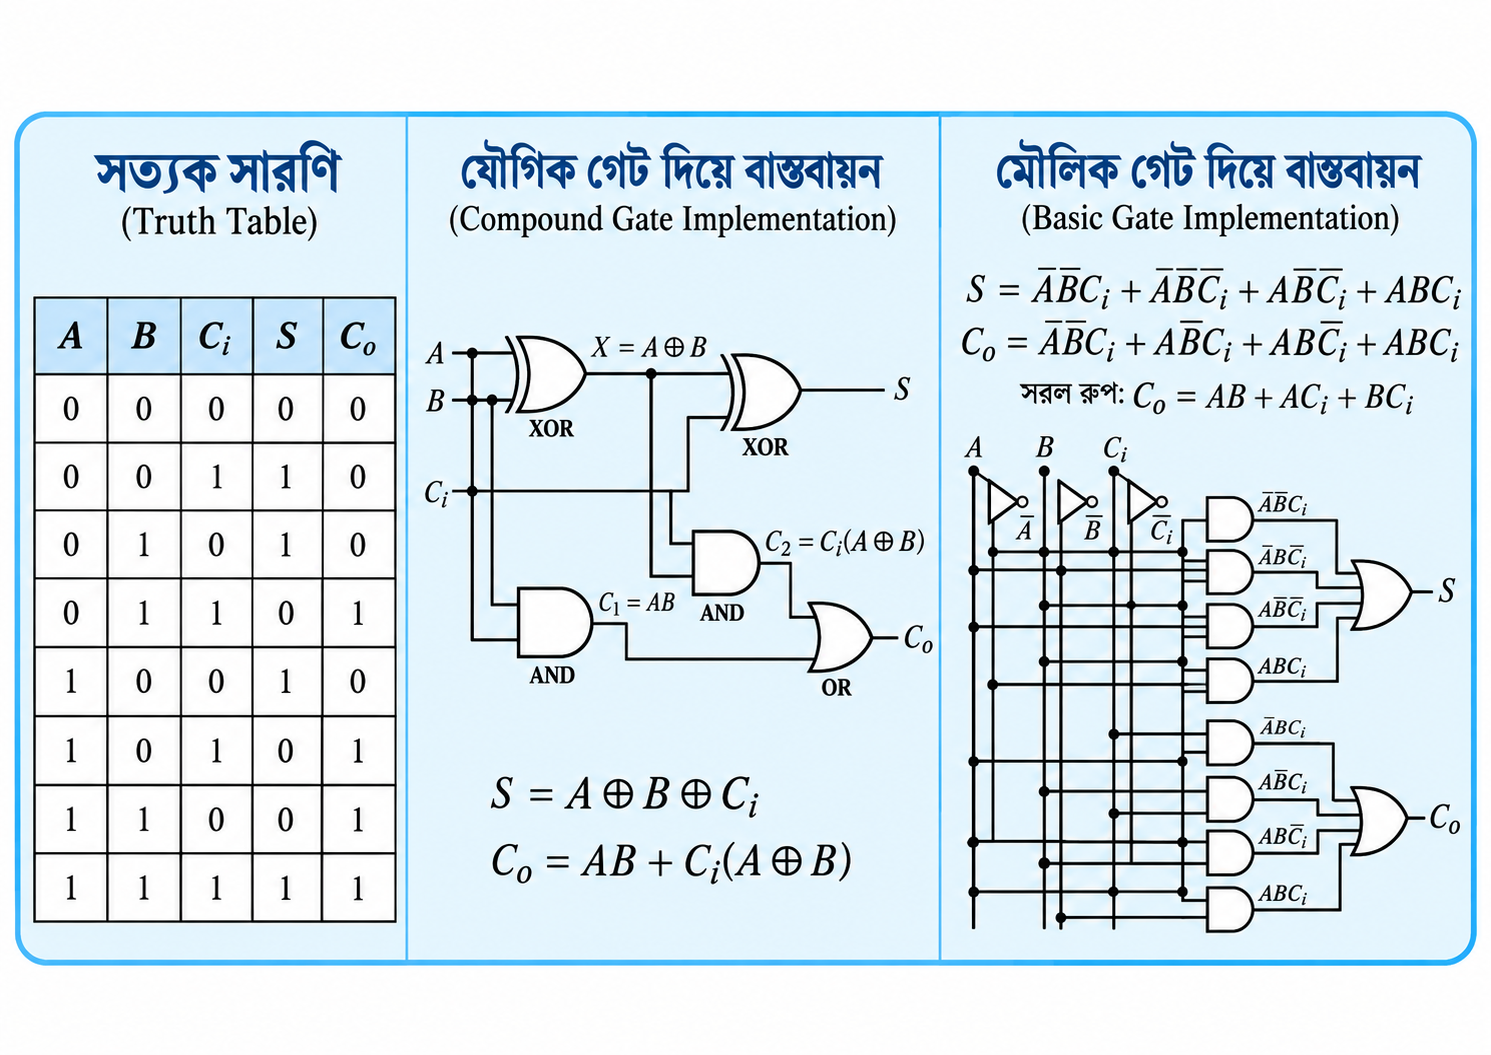
\includegraphics[width=\textwidth]{chapters/Chapter03/resources/images/full_adder_box.png}

\smallskip
{\small \textbf{চিত্র:} পূর্ণযোগকের সত্যক সারণি, যৌগিক গেট দিয়ে বাস্তবায়ন এবং মৌলিক গেট দিয়ে বাস্তবায়ন}
\end{center}

% =========================================================
% Boolean expressions of Full Adder
% =========================================================

\paragraph{যোগফল \(S\)-এর বুলিয়ান রাশি নির্ণয়:}

সত্যক সারণি থেকে দেখা যায়, \(S=1\) হয় নিম্নোক্ত ইনপুটের জন্য:
\[
001,\;010,\;100,\;111
\]

অতএব,
\[
\begin{aligned}
S &=
\overline{A}\,\overline{B}\,C_i
+\overline{A}\,B\,\overline{C_i}
+A\,\overline{B}\,\overline{C_i}
+A\,B\,C_i \\[4pt]
&=
\overline{A}\left(\overline{B}C_i+B\overline{C_i}\right)
+A\left(\overline{B}\,\overline{C_i}+BC_i\right) \\[4pt]
&=
\overline{A}(B\oplus C_i)+A\overline{(B\oplus C_i)} \\[4pt]
&=
A\oplus(B\oplus C_i) \\[4pt]
&=
A\oplus B\oplus C_i
\end{aligned}
\]

সুতরাং,
\[
\boxed{S=A\oplus B\oplus C_i}
\]

\paragraph{ক্যারি \(C_o\)-এর বুলিয়ান রাশি নির্ণয়:}

সত্যক সারণি থেকে দেখা যায়, \(C_o=1\) হয় নিম্নোক্ত ইনপুটের জন্য:
\[
011,\;101,\;110,\;111
\]

অতএব,
\[
\begin{aligned}
C_o &=
\overline{A}BC_i
+A\overline{B}C_i
+AB\overline{C_i}
+ABC_i \\[4pt]
&=
\overline{A}BC_i
+A\overline{B}C_i
+AB(\overline{C_i}+C_i) \\[4pt]
&=
\overline{A}BC_i
+A\overline{B}C_i
+AB \\[4pt]
&=
C_i(\overline{A}B+A\overline{B})+AB \\[4pt]
&=
C_i(A\oplus B)+AB
\end{aligned}
\]

অর্থাৎ,
\[
\boxed{C_o=AB+C_i(A\oplus B)}
\]

এখন এটিকে আরও পরিচিত রূপে লেখা যায়—
\[
\begin{aligned}
C_o &= AB+C_i(A\oplus B) \\[4pt]
&= AB+C_i(\overline{A}B+A\overline{B}) \\[4pt]
&= AB+\overline{A}BC_i+A\overline{B}C_i \\[4pt]
&= AB+BC_i+AC_i
\end{aligned}
\]

সুতরাং,
\[
\boxed{C_o=AB+AC_i+BC_i}
\]

\par\begingroup

\textbf{পূর্ণযোগকের দুটি গুরুত্বপূর্ণ সূত্র:}
\[
S=A\oplus B\oplus C_i
\]
\[
C_o=AB+C_i(A\oplus B)
\]
অথবা,
\[
C_o=AB+AC_i+BC_i
\]
\par\endgroup


% =========================================================
% 3.10.4 Full Adder using two Half Adders
% =========================================================

\subsubsection*{অর্ধযোগক ও পূর্ণযোগকের পার্থক্য}

\begin{center}
\renewcommand{\arraystretch}{1.35}
\begin{tabular}{|p{0.20\linewidth}|p{0.34\linewidth}|p{0.34\linewidth}|}
\hline
\rowcolor{gray!15}
\textbf{বিষয়} & \textbf{অর্ধযোগক (\textenglish{Half Adder})} & \textbf{পূর্ণযোগক (\textenglish{Full Adder})} \\
\hline
ইনপুট সংখ্যা & ২টি & ৩টি \\
\hline
ইনপুট & \(A,B\) & \(A,B,C_i\) \\
\hline
ক্যারি ইনপুট & নেই & আছে \\
\hline
আউটপুট & \(S,C\) & \(S,C_o\) \\
\hline
ব্যবহার & দুটি ১-বিট সংখ্যা যোগ করে & ক্যারিসহ দুটি ১-বিট সংখ্যা যোগ করে \\
\hline
গঠন & \textenglish{XOR} ও \textenglish{AND} গেট & \textenglish{XOR}, \textenglish{AND} ও \textenglish{OR} গেট \\
\hline
\end{tabular}
\end{center}

% =========================================================
% 3.10.6 Applications
% =========================================================

\subsubsection*{অ্যাডারের ব্যবহার}

অ্যাডার ডিজিটাল ইলেকট্রনিক্স ও কম্পিউটার ব্যবস্থায় অত্যন্ত গুরুত্বপূর্ণ।
এর কয়েকটি ব্যবহার হলো—

\begin{enumerate}
    \item \textenglish{ALU} (\textenglish{Arithmetic Logic Unit})-তে বাইনারি যোগের কাজে।
    \item বহু-বিট বাইনারি সংখ্যা যোগ করতে।
    \item কম্পিউটার প্রসেসরের গাণিতিক অংশে।
    \item ডিজিটাল ক্যালকুলেটরে।
    \item বিভিন্ন ডিজিটাল সার্কিটে \textenglish{sum} ও \textenglish{carry} নির্ণয়ে।
\end{enumerate}

\par\begingroup

\textbf{পরীক্ষার জন্য খুব গুরুত্বপূর্ণ:}
\begin{itemize}[label={{\bulletfont\textbullet}}, leftmargin=*, nosep]
    \item \textbf{Half Adder:}
    \[
    S=A\oplus B,\qquad C=AB
    \]

    \item \textbf{Full Adder:}
    \[
    S=A\oplus B\oplus C_i
    \]
    \[
    C_o=AB+C_i(A\oplus B)
    \]
    অথবা,
    \[
    C_o=AB+AC_i+BC_i
    \]
\end{itemize}
\par\endgroup

% =========================================================
% 3.10.4 দুটি অর্ধযোগক দিয়ে পূর্ণযোগক
% =========================================================

\subsection{দুটি অর্ধযোগক দিয়ে পূর্ণযোগক
(\textenglish{Full Adder Using Two Half Adders})}

আমরা জানি, \textenglish{Full Adder}-এ তিনটি ইনপুট থাকে— \(A\), \(B\) এবং \(C_i\)।
এদের যোগফল নির্ণয়ের জন্য দুটি \textenglish{Half Adder} এবং একটি \textenglish{OR Gate}
ব্যবহার করা যায়। এই পদ্ধতিটি খুবই গুরুত্বপূর্ণ, কারণ এর মাধ্যমে বোঝা যায়
কীভাবে একটি তুলনামূলক জটিল সার্কিটকে সহজ সার্কিটের সমন্বয়ে গঠন করা সম্ভব।

\subsubsection*{কার্যপ্রণালি
(\textenglish{Working Principle})}

প্রথম \textenglish{Half Adder}-এ \(A\) ও \(B\) ইনপুট দেওয়া হয়।

তাহলে প্রথম \textenglish{Half Adder} থেকে পাই—

\[
S_1=A\oplus B
\]

এবং,

\[
C_1=AB
\]

এরপর দ্বিতীয় \textenglish{Half Adder}-এ প্রথম \textenglish{Half Adder}-এর
যোগফল \(S_1\) এবং তৃতীয় ইনপুট \(C_i\) দেওয়া হয়।

তাহলে দ্বিতীয় \textenglish{Half Adder} থেকে পাই—

\[
S=S_1\oplus C_i
\]

অতএব,

\[
S=(A\oplus B)\oplus C_i
\]

সুতরাং,

\[
\boxed{S=A\oplus B\oplus C_i}
\]

আবার, দ্বিতীয় \textenglish{Half Adder}-এর ক্যারি হবে—

\[
C_2=S_1C_i
\]

এখন \(S_1=A\oplus B\) বসালে পাই—

\[
C_2=(A\oplus B)C_i
\]

এখন পূর্ণযোগকের চূড়ান্ত ক্যারি আউট হবে প্রথম ও দ্বিতীয়
\textenglish{Half Adder}-এর ক্যারির \textenglish{OR}।

অর্থাৎ,

\[
C_o=C_1+C_2
\]

এখন \(C_1=AB\) এবং \(C_2=(A\oplus B)C_i\) বসালে পাই—

\[
C_o=AB+(A\oplus B)C_i
\]

এখন \((A\oplus B)\)-এর মান বসাই—

\[
A\oplus B=\overline{A}B+A\overline{B}
\]

সুতরাং,

\[
C_o=AB+(\overline{A}B+A\overline{B})C_i
\]

\[
=AB+\overline{A}BC_i+A\overline{B}C_i
\]

এখন \textenglish{Boolean Algebra} ব্যবহার করে পূর্ণযোগকের বহুল ব্যবহৃত রূপ পাওয়া যায়—

\[
\boxed{C_o=AB+AC_i+BC_i}
\]

অতএব, দুটি \textenglish{Half Adder} এবং একটি \textenglish{OR Gate}
ব্যবহার করে \textenglish{Full Adder} বাস্তবায়ন করা যায়।

\subsubsection*{সারসংক্ষেপ
(\textenglish{Summary})}

\[
\boxed{S=A\oplus B\oplus C_i}
\]

\[
\boxed{C_o=AB+(A\oplus B)C_i}
\]

এবং সমতুল্যভাবে,

\[
\boxed{C_o=AB+AC_i+BC_i}
\]

\par\begingroup

\textbf{মনে রাখবে:}
দুটি \textenglish{Half Adder} দিয়ে \textenglish{Full Adder} তৈরি করলে
প্রথম \textenglish{Half Adder} \(A\) ও \(B\) যোগ করে,
দ্বিতীয় \textenglish{Half Adder} \(S_1\) ও \(C_i\) যোগ করে,
এবং দুটি ক্যারি \textenglish{OR} করে চূড়ান্ত \(C_o\) পাওয়া যায়।
\par\endgroup


\begin{figure}[!htbp]
    \centering
    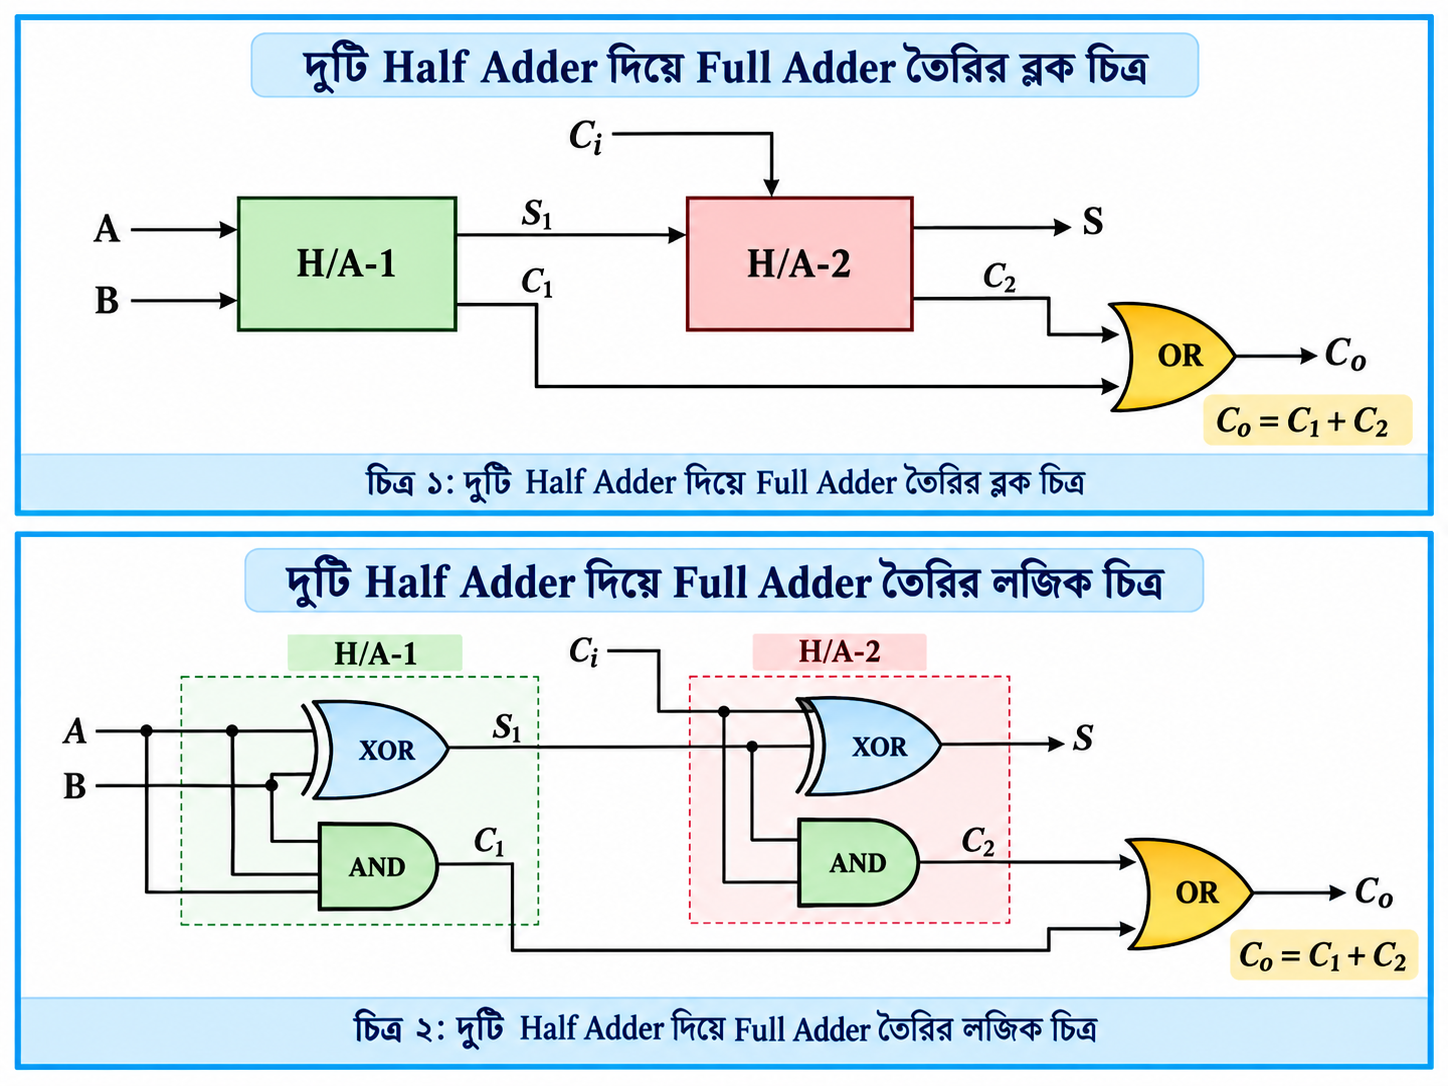
\includegraphics[width=0.92\textwidth]{chapters/Chapter03/resources/images/half_to_full_adder.png}
    \caption*{চিত্র: দুটি \textenglish{Half Adder} এবং একটি \textenglish{OR Gate} ব্যবহার করে \textenglish{Full Adder} বাস্তবায়ন}
\end{figure}


% =========================================================
% 3.10.5 সার্বজনীন গেট দিয়ে পূর্ণযোগক বাস্তবায়ন
% =========================================================

\subsection{সার্বজনীন গেট দিয়ে পূর্ণযোগক বাস্তবায়ন
(\textenglish{Implementation of Full Adder Using Universal Gates})}

আমরা জানি, \textenglish{NAND} ও \textenglish{NOR} গেটকে
সার্বজনীন গেট (\textenglish{Universal Gate}) বলা হয়।
কারণ, এই গেটগুলোর যেকোনো এক ধরনের গেট ব্যবহার করে
যেকোনো \textenglish{Boolean Function} বাস্তবায়ন করা সম্ভব।
সুতরাং \textenglish{Full Adder}-ও শুধু \textenglish{NAND} গেট
অথবা শুধু \textenglish{NOR} গেট ব্যবহার করে তৈরি করা যায়।

\subsubsection*{পূর্ণযোগকের মৌলিক সমীকরণ
(\textenglish{Basic Equations of Full Adder})}

পূর্ণযোগকের তিনটি ইনপুট \(A\), \(B\) ও \(C_i\)-এর জন্য
যোগফল \(S\) এবং ক্যারি আউট \(C_o\) নির্ণয়ের সমীকরণ হলো—

\[
S=A\oplus B\oplus C_i
\]

\[
C_o=AB+AC_i+BC_i
\]

এখন এই সমীকরণগুলোকে এমনভাবে রূপান্তর করা হয়,
যাতে শুধু \textenglish{NAND} বা শুধু \textenglish{NOR} গেট ব্যবহার করে
বাস্তবায়ন করা যায়।

\subsubsection*{\textenglish{NOR} গেট দিয়ে বাস্তবায়নের ধারণা}

\textenglish{NOR} গেট দিয়ে বাস্তবায়নের ক্ষেত্রে
সাধারণত \textenglish{OR} এবং \textenglish{NOT} অপারেশনের উপযোগী রূপে
সমীকরণকে পরিবর্তন করা হয়। \textenglish{De Morgan's Theorem} ব্যবহার করে
বিভিন্ন ধাপে রাশিকে \textenglish{NOR}-উপযোগী আকারে লেখা হয়।
এরপর প্রাপ্ত রাশি অনুযায়ী লজিক সার্কিট আঁকা হয়।

\subsubsection*{\textenglish{NAND} গেট দিয়ে বাস্তবায়নের ধারণা}

\textenglish{NAND} গেট দিয়ে বাস্তবায়নের ক্ষেত্রে
সমীকরণকে এমনভাবে ভেঙে লেখা হয়, যাতে
\textenglish{AND} এবং \textenglish{NOT}-নির্ভর রূপ থেকে
শুধু \textenglish{NAND} গেট ব্যবহার করে আউটপুট তৈরি করা যায়।
এক্ষেত্রেও \textenglish{Boolean Algebra} ও \textenglish{De Morgan's Theorem}
খুব গুরুত্বপূর্ণ ভূমিকা রাখে।

\subsubsection*{কেন এটি গুরুত্বপূর্ণ?}

সার্বজনীন গেট দিয়ে \textenglish{Full Adder} বাস্তবায়ন গুরুত্বপূর্ণ, কারণ—

\begin{enumerate}
    \item একটি নির্দিষ্ট ধরনের গেট ব্যবহার করে সম্পূর্ণ সার্কিট তৈরি করা যায়।
    \item \textenglish{IC} ডিজাইনে একই ধরনের গেট ব্যবহার করলে নকশা সহজ হয়।
    \item সার্কিট বিশ্লেষণ ও বাস্তবায়নের দক্ষতা বাড়ে।
    \item \textenglish{Boolean Algebra} ও \textenglish{Gate Realization}-এর সম্পর্ক স্পষ্ট হয়।
\end{enumerate}

\par\begingroup

\textbf{মনে রাখবে:}
\textenglish{Full Adder} বাস্তবায়নে \textenglish{NAND} ও \textenglish{NOR}—
উভয় ধরনের সার্বজনীন গেটই ব্যবহার করা যায়।
বোর্ড পরীক্ষায় অনেক সময় সমীকরণ এবং সার্কিট—দুটিই চাওয়া হয়।
\par\endgroup


\begin{figure}[!htbp]
    \centering
    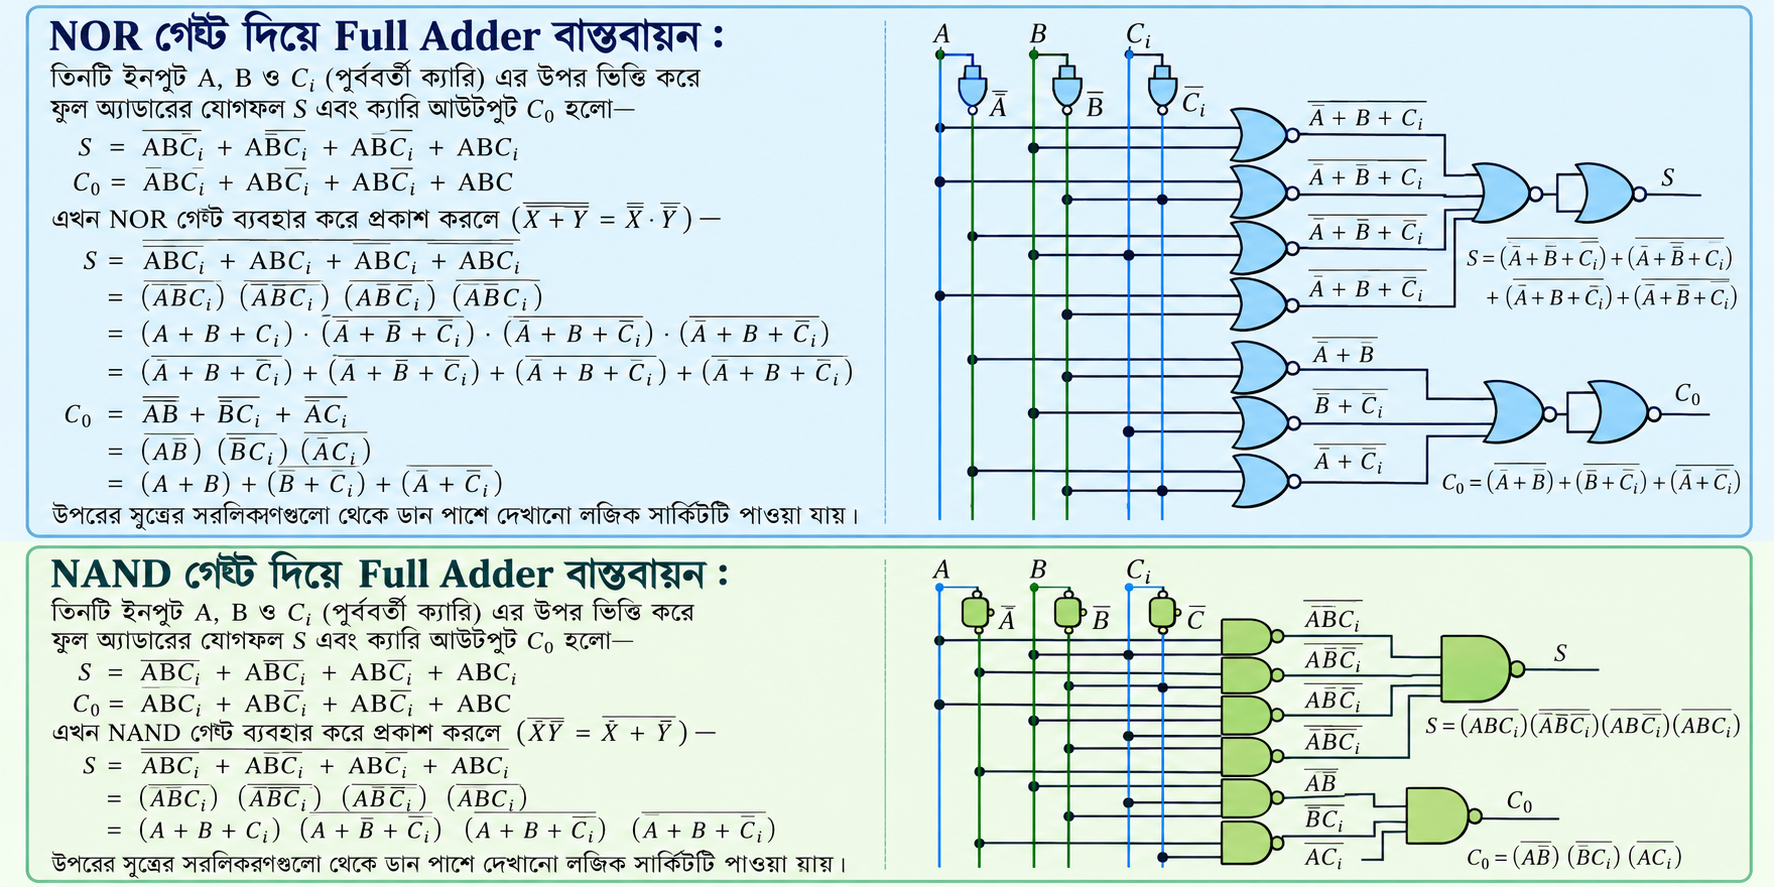
\includegraphics[width=\textwidth]{chapters/Chapter03/resources/images/nand_nor_full_adder.png}
    \caption*{চিত্র: \textenglish{NOR} এবং \textenglish{NAND} গেট ব্যবহার করে \textenglish{Full Adder} বাস্তবায়ন}
\end{figure}

\subsection{নয়টি দুই-ইনপুট গেটে পূর্ণযোগকের ধাপ}
নিচের মধ্যবর্তী সংকেতগুলো অনুসরণ করলে শুধু একই ধরনের গেট দিয়ে যোগফল ও ক্যারি তৈরি করা যায়। $C_i$ ক্যারি ইনপুট এবং $C_o$ ক্যারি আউটপুট।

\smallhead{শুধু NAND}
\[\begin{aligned}
P&=\overline{AB},&Q&=\overline{AP},&R&=\overline{BP},\\
X&=\overline{QR},&U&=\overline{XC_i},&V&=\overline{XU},\\
W&=\overline{C_iU},&S&=\overline{VW},&C_o&=\overline{PU}.
\end{aligned}\]
প্রথম চার গেটে $X=A\oplus B$। পরের চার গেটে $S=X\oplus C_i$। শেষ গেটে $C_o=\overline{\overline{AB}\cdot\overline{XC_i}}=AB+XC_i$। অতএব একই নয় গেটের সংযোগ পূর্ণযোগক।

\smallhead{শুধু NOR}
\[\begin{aligned}
P&=\overline{A+B},&Q&=\overline{A+P},&R&=\overline{B+P},\\
X&=\overline{Q+R},&U&=\overline{X+C_i},&V&=\overline{X+U},\\
W&=\overline{C_i+U},&S&=\overline{V+W},&C_o&=\overline{P+U}.
\end{aligned}\]
প্রথম চার গেটে X হলো A ও B-এর XNOR। পরের চার গেট X ও $C_i$-এর XNOR করলে দুইবার পূরক হয়ে $S=A\oplus B\oplus C_i$ পাওয়া যায়। শেষ NOR-এর ফল $C_o=(A+B)(X+C_i)=AB+AC_i+BC_i$। এখানে X-এর অর্থ NAND নির্মাণের X থেকে আলাদা।

\chThreeExample{১}{দুই half adder-এর মধ্যবর্তী মান}
$A=1,B=0,C_i=1$।
\chThreeAnswer প্রথম half adder-এ $S_1=1,C_1=0$। দ্বিতীয়টিতে $S=S_1\oplus C_i=0,C_2=S_1C_i=1$। শেষ OR-এ $C_o=C_1+C_2=1$। ফল $C_oS=10_2$, যা $1+0+1$-এর সঠিক যোগফল।

\chThreeExample{২}{অ্যাডার দিয়ে বিয়োগ}
চার বিটে $9-5$ নির্ণয় করতে $A=1001$, $B=0101$।
\chThreeAnswer B-এর বিট উল্টে $1010$ এবং প্রথম carry-in ১ দাও।
\[1001+1010+1=1\;0100.\]
অতিরিক্ত ক্যারি বাদ দিলে চার বিটে $0100=4$। এই উদাহরণে A ও B চিহ্নবিহীন মান; চার বিট signed হিসেবে ৯ লেখা যায় না।


% =========================================================
% 3.10.6 Binary Adder
% =========================================================

\subsection{বাইনারি অ্যাডার
(\textenglish{Binary Adder})}

\textenglish{Half Adder} ও \textenglish{Full Adder} মূলত এক-বিট
বাইনারি সংখ্যা যোগ করার মৌলিক সার্কিট। কিন্তু কম্পিউটারে সাধারণত
\(4\)-\textenglish{bit}, \(8\)-\textenglish{bit},
\(16\)-\textenglish{bit}, \(32\)-\textenglish{bit} ইত্যাদি বহু-বিট
সংখ্যা নিয়ে কাজ করতে হয়।

যেমন,

\[
(1011)_2+(0110)_2
\]

যোগ করতে হলে শুধু এক জোড়া \textenglish{bit} যোগ করলেই হবে না।
প্রতিটি \textenglish{bit-position}-এর \textenglish{bit} যোগ করতে হবে
এবং এক ধাপে উৎপন্ন \textenglish{Carry} পরবর্তী ধাপে পাঠাতে হবে।

একাধিক \textenglish{bit}-এর দুটি বাইনারি সংখ্যা যোগ করার জন্য
একাধিক \textenglish{Adder} প্রয়োজনমতো সংযুক্ত করে যে সার্কিট তৈরি করা হয়,
তাকে \textbf{\textenglish{Binary Adder}} বলে।

\subsubsection*{সহজভাবে}

\[
\boxed{
\text{\textenglish{Multi-bit Binary Numbers}}
\rightarrow
\text{\textenglish{Binary Adder}}
\rightarrow
\text{\textenglish{Sum + Final Carry}}
}
\]


% =========================================================
% Types of Binary Adder
% =========================================================

\subsection{বাইনারি অ্যাডারের প্রকারভেদ}

বাইনারি সংখ্যার বিটগুলো কীভাবে অ্যাডারে প্রবেশ করে এবং কীভাবে যোগ
সম্পন্ন হয়, তার ভিত্তিতে \textenglish{Binary Adder} প্রধানত দুই প্রকার—

\begin{enumerate}[leftmargin=*,itemsep=2pt]
    \item \textbf{\textenglish{Serial Binary Adder}}
    \item \textbf{\textenglish{Parallel Binary Adder}}
\end{enumerate}


% =========================================================
% Serial Binary Adder
% =========================================================

\paragraph{\textenglish{Serial Binary Adder}:}

যে বাইনারি অ্যাডারে দুটি বহু-বিট বাইনারি সংখ্যার সংশ্লিষ্ট বিটগুলো
একটির পর একটি ধারাবাহিকভাবে যোগ করা হয়,
তাকে \textenglish{Serial Binary Adder} বলে।

এখানে সাধারণত একটি \textenglish{Full Adder} ব্যবহার করে
প্রতিটি ধাপে এক জোড়া বিট যোগ করা হয়।
এক ধাপে উৎপন্ন \textenglish{Carry} পরবর্তী ধাপের জন্য সংরক্ষণ করা হয়।

ধরা যাক,

\[
A=A_3A_2A_1A_0
\]

এবং,

\[
B=B_3B_2B_1B_0
\]

তাহলে পর্যায়ক্রমে যোগ হবে—

\[
A_0+B_0+C_0
\]

\[
A_1+B_1+C_1
\]

\[
A_2+B_2+C_2
\]

\[
A_3+B_3+C_3
\]

\par\begingroup

\textbf{মনে রাখবে:}
\textenglish{Serial Binary Adder}-এ একই \textenglish{Full Adder}
বারবার ব্যবহার করে একটির পর একটি বিট যোগ করা যায়।
তাই হার্ডওয়্যার কম লাগে, কিন্তু যোগ সম্পন্ন করতে তুলনামূলক বেশি সময় লাগে।
\par\endgroup



% =========================================================
% Parallel Binary Adder
% =========================================================

\paragraph{\textenglish{Parallel Binary Adder}:}

যে বাইনারি অ্যাডারে দুটি বহু-বিট বাইনারি সংখ্যার সংশ্লিষ্ট বিটগুলো
একই সময়ে পৃথক \textenglish{Adder stage}-এ প্রবেশ করে,
তাকে \textenglish{Parallel Binary Adder} বলে।

প্রতিটি \textenglish{bit-position}-এর জন্য আলাদা
\textenglish{Full Adder} ব্যবহার করা হয়।

যেমন, দুটি \(4\)-\textenglish{bit} বাইনারি সংখ্যা যোগ করতে
চারটি \textenglish{Full Adder} ধারাবাহিকভাবে সংযুক্ত করা যায়।


% =========================================================
% 4-bit Parallel Binary Adder
% =========================================================

\subsubsection*{৪-বিট প্যারালাল বাইনারি অ্যাডার
(\textenglish{4-bit Parallel Binary Adder})}

ধরা যাক, দুটি \(4\)-\textenglish{bit} বাইনারি সংখ্যা—

\[
A_3A_2A_1A_0
\]

এবং,

\[
B_3B_2B_1B_0
\]

যোগ করতে হবে।

এক্ষেত্রে চারটি \textenglish{Full Adder} ব্যবহার করা হয়।
সর্বডানের \textenglish{Full Adder} সর্বনিম্ন গুরুত্বপূর্ণ বিট
(\textenglish{LSB}) এবং সর্ববামের \textenglish{Full Adder}
সর্বাধিক গুরুত্বপূর্ণ বিট (\textenglish{MSB}) যোগ করে।

প্রাথমিকভাবে \textenglish{Carry-in} না থাকলে—

\[
C_0=0
\]

ধরা হয়।

প্রতিটি ধাপে—

\[
FA_0:
A_0+B_0+C_0
\longrightarrow
S_0,\;C_1
\]

\[
FA_1:
A_1+B_1+C_1
\longrightarrow
S_1,\;C_2
\]

\[
FA_2:
A_2+B_2+C_2
\longrightarrow
S_2,\;C_3
\]

\[
FA_3:
A_3+B_3+C_3
\longrightarrow
S_3,\;C_4
\]

অতএব সম্পূর্ণ ফলাফল—

\[
\boxed{C_4S_3S_2S_1S_0}
\]


% =========================================================
% 4-bit Parallel Binary Adder Diagram
% =========================================================

\begin{center}

\begin{chThreeDiagram}
\begin{tikzpicture}[
    >=Stealth,
    line width=0.8pt,
    fa/.style={
        draw,
        rounded corners=2pt,
        fill=ICTLightBlue,
        minimum width=2.25cm,
        minimum height=1.15cm,
        align=center
    }
]

\node[fa] (fa3) at (0,0) {\textbf{\(FA_3\)}};
\node[fa] (fa2) at (3.6,0) {\textbf{\(FA_2\)}};
\node[fa] (fa1) at (7.2,0) {\textbf{\(FA_1\)}};
\node[fa] (fa0) at (10.8,0) {\textbf{\(FA_0\)}};

% A3, B3
\draw[->] (-0.55,2.0) -- (-0.55,0.62);
\node[above] at (-0.55,2.0) {\(A_3\)};

\draw[->] (0.55,2.0) -- (0.55,0.62);
\node[above] at (0.55,2.0) {\(B_3\)};

% A2, B2
\draw[->] (3.05,2.0) -- (3.05,0.62);
\node[above] at (3.05,2.0) {\(A_2\)};

\draw[->] (4.15,2.0) -- (4.15,0.62);
\node[above] at (4.15,2.0) {\(B_2\)};

% A1, B1
\draw[->] (6.65,2.0) -- (6.65,0.62);
\node[above] at (6.65,2.0) {\(A_1\)};

\draw[->] (7.75,2.0) -- (7.75,0.62);
\node[above] at (7.75,2.0) {\(B_1\)};

% A0, B0
\draw[->] (10.25,2.0) -- (10.25,0.62);
\node[above] at (10.25,2.0) {\(A_0\)};

\draw[->] (11.35,2.0) -- (11.35,0.62);
\node[above] at (11.35,2.0) {\(B_0\)};

% Carry chain
\draw[<-] (fa3.west) -- ++(-1.25,0);
\node[above] at (-1.75,0.08) {\(C_4\)};

\draw[<-] (fa3.east) -- (fa2.west);
\node[above] at (1.8,0.08) {\(C_3\)};

\draw[<-] (fa2.east) -- (fa1.west);
\node[above] at (5.4,0.08) {\(C_2\)};

\draw[<-] (fa1.east) -- (fa0.west);
\node[above] at (9.0,0.08) {\(C_1\)};

\draw[<-] (fa0.east) -- ++(1.30,0);
\node[above] at (12.55,0.08) {\(C_0=0\)};

% Sum outputs
\draw[->] (fa3.south) -- ++(0,-1.15);
\node[below] at (0,-1.15) {\(S_3\)};

\draw[->] (fa2.south) -- ++(0,-1.15);
\node[below] at (3.6,-1.15) {\(S_2\)};

\draw[->] (fa1.south) -- ++(0,-1.15);
\node[below] at (7.2,-1.15) {\(S_1\)};

\draw[->] (fa0.south) -- ++(0,-1.15);
\node[below] at (10.8,-1.15) {\(S_0\)};

\end{tikzpicture}
\end{chThreeDiagram}

\end{center}

\[
\boxed{
\text{\textenglish{Output}}
=
C_4S_3S_2S_1S_0
}
\]

এখানে \(A_3A_2A_1A_0\) এবং \(B_3B_2B_1B_0\) হলো দুটি
\(4\)-\textenglish{bit} বাইনারি সংখ্যা।
\(S_3S_2S_1S_0\) হলো চারটি \textenglish{Sum bit}
এবং \(C_4\) হলো চূড়ান্ত \textenglish{Carry}।


% =========================================================
% Carry Propagation
% =========================================================

\subsubsection*{ক্যারি প্রবাহ
(\textenglish{Carry Propagation})}

প্রতিটি \textenglish{Full Adder}-এর \textenglish{Carry-out}
পরবর্তী \textenglish{Full Adder}-এর \textenglish{Carry-in}
হিসেবে প্রবেশ করে।

অর্থাৎ,

\[
C_0
\rightarrow
FA_0
\rightarrow
C_1
\rightarrow
FA_1
\rightarrow
C_2
\rightarrow
FA_2
\rightarrow
C_3
\rightarrow
FA_3
\rightarrow
C_4
\]

এইভাবে \textenglish{Carry} এক \textenglish{stage} থেকে
পরবর্তী \textenglish{stage}-এ ক্রমান্বয়ে ছড়িয়ে যায়।

এই কারণে এ ধরনের সাধারণ \textenglish{Parallel Adder}-কে
\textenglish{Ripple Carry Adder}-ও বলা হয়।

\par\begingroup

\textbf{মনে রাখবে:}
\textenglish{Parallel Adder}-এ \textenglish{input bit}গুলো একই সময়ে
সংশ্লিষ্ট \textenglish{Full Adder}-এ প্রবেশ করলেও
\textenglish{Carry} এক \textenglish{stage} থেকে পরবর্তী
\textenglish{stage}-এ ধারাবাহিকভাবে প্রবাহিত হয়।
\par\endgroup



% =========================================================
% Example: 1011 + 1111
% =========================================================

\subsubsection*{উদাহরণ:
\((1011)_2+(1111)_2\)}

ধরা যাক,

\[
A=(1011)_2
\]

এবং,

\[
B=(1111)_2
\]

তাহলে—

\[
A_3A_2A_1A_0=1011
\]

এবং,

\[
B_3B_2B_1B_0=1111
\]

প্রাথমিক \textenglish{Carry}—

\[
C_0=0
\]


% =========================================================
% Example Diagram
% =========================================================

\begin{center}

\begin{chThreeDiagram}
\begin{tikzpicture}[
    >=Stealth,
    line width=0.8pt,
    fa/.style={
        draw,
        rounded corners=2pt,
        fill=ICTLightGreen,
        minimum width=2.25cm,
        minimum height=1.15cm,
        align=center
    }
]

\node[fa] (fa3) at (0,0) {\textbf{\(FA_3\)}};
\node[fa] (fa2) at (3.6,0) {\textbf{\(FA_2\)}};
\node[fa] (fa1) at (7.2,0) {\textbf{\(FA_1\)}};
\node[fa] (fa0) at (10.8,0) {\textbf{\(FA_0\)}};

% FA3
\node[above] at (-0.55,2.0) {\(A_3=1\)};
\node[above] at (0.60,2.0) {\(B_3=1\)};
\draw[->] (-0.55,1.72) -- (-0.55,0.62);
\draw[->] (0.60,1.72) -- (0.60,0.62);

% FA2
\node[above] at (3.05,2.0) {\(A_2=0\)};
\node[above] at (4.20,2.0) {\(B_2=1\)};
\draw[->] (3.05,1.72) -- (3.05,0.62);
\draw[->] (4.20,1.72) -- (4.20,0.62);

% FA1
\node[above] at (6.65,2.0) {\(A_1=1\)};
\node[above] at (7.80,2.0) {\(B_1=1\)};
\draw[->] (6.65,1.72) -- (6.65,0.62);
\draw[->] (7.80,1.72) -- (7.80,0.62);

% FA0
\node[above] at (10.25,2.0) {\(A_0=1\)};
\node[above] at (11.40,2.0) {\(B_0=1\)};
\draw[->] (10.25,1.72) -- (10.25,0.62);
\draw[->] (11.40,1.72) -- (11.40,0.62);

% Carry values
\draw[<-] (fa3.west) -- ++(-1.20,0);
\node[above] at (-1.70,0.08) {\(C_4=1\)};

\draw[<-] (fa3.east) -- (fa2.west);
\node[above] at (1.80,0.08) {\(C_3=1\)};

\draw[<-] (fa2.east) -- (fa1.west);
\node[above] at (5.40,0.08) {\(C_2=1\)};

\draw[<-] (fa1.east) -- (fa0.west);
\node[above] at (9.00,0.08) {\(C_1=1\)};

\draw[<-] (fa0.east) -- ++(1.20,0);
\node[above] at (12.50,0.08) {\(C_0=0\)};

% Sum outputs
\draw[->] (fa3.south) -- ++(0,-1.15);
\node[below] at (0,-1.15) {\(S_3=1\)};

\draw[->] (fa2.south) -- ++(0,-1.15);
\node[below] at (3.6,-1.15) {\(S_2=0\)};

\draw[->] (fa1.south) -- ++(0,-1.15);
\node[below] at (7.2,-1.15) {\(S_1=1\)};

\draw[->] (fa0.south) -- ++(0,-1.15);
\node[below] at (10.8,-1.15) {\(S_0=0\)};

\end{tikzpicture}
\end{chThreeDiagram}

\end{center}


% =========================================================
% Stage-by-stage Calculation
% =========================================================

\par\begingroup


\begin{minipage}[t]{0.235\textwidth}
\centering

\textbf{স্টেজ–০}\\[-1mm]
{\footnotesize \textenglish{LSB}}

\vspace{2mm}

\[
A_0=1,\quad B_0=1
\]

\[
C_0=0
\]

\[
1+1+0=10
\]

\[
\boxed{S_0=0,\;C_1=1}
\]

\end{minipage}
\hfill
\begin{minipage}[t]{0.235\textwidth}
\centering

\textbf{স্টেজ–১}

\vspace{4mm}

\[
A_1=1,\quad B_1=1
\]

\[
C_1=1
\]

\[
1+1+1=11
\]

\[
\boxed{S_1=1,\;C_2=1}
\]

\end{minipage}
\hfill
\begin{minipage}[t]{0.235\textwidth}
\centering

\textbf{স্টেজ–২}

\vspace{4mm}

\[
A_2=0,\quad B_2=1
\]

\[
C_2=1
\]

\[
0+1+1=10
\]

\[
\boxed{S_2=0,\;C_3=1}
\]

\end{minipage}
\hfill
\begin{minipage}[t]{0.235\textwidth}
\centering

\textbf{স্টেজ–৩}\\[-1mm]
{\footnotesize \textenglish{MSB}}

\vspace{2mm}

\[
A_3=1,\quad B_3=1
\]

\[
C_3=1
\]

\[
1+1+1=11
\]

\[
\boxed{S_3=1,\;C_4=1}
\]

\end{minipage}

\par\endgroup

অতএব,

\[
C_4S_3S_2S_1S_0=11010
\]

সুতরাং,

\[
\boxed{
(1011)_2+(1111)_2=(11010)_2
}
\]

দশমিক পদ্ধতিতে যাচাই করলে—

\[
(1011)_2=(11)_{10}
\]

এবং,

\[
(1111)_2=(15)_{10}
\]

তাই,

\[
11+15=26
\]

এবং,

\[
(26)_{10}=(11010)_2
\]

অতএব ফল সঠিক।


% =========================================================
% Serial vs Parallel Comparison
% =========================================================

\subsubsection*{\textenglish{Serial} ও \textenglish{Parallel Binary Adder}-এর পার্থক্য}

\begin{center}

\renewcommand{\arraystretch}{1.25}

\begin{tabularx}
{\textwidth}
{|L{0.20\textwidth}|Y|Y|}

\hline

\rowcolor{ICTLightBlue}

\textbf{বিষয়}
&
\textbf{\textenglish{Serial Binary Adder}}
&
\textbf{\textenglish{Parallel Binary Adder}}
\\
\hline

যোগের পদ্ধতি
&
বিট একটির পর একটি যোগ করা হয়।
&
সংশ্লিষ্ট বিটগুলো একই সময়ে পৃথক
\textenglish{Adder}-এ প্রবেশ করে।
\\
\hline

\textenglish{Adder} সংখ্যা
&
তুলনামূলক কম।
&
তুলনামূলক বেশি।
\\
\hline

৪-বিট যোগে
&
সাধারণত একই \textenglish{Full Adder} বারবার ব্যবহার করা হয়।
&
সাধারণত ৪টি \textenglish{Full Adder} ব্যবহার করা হয়।
\\
\hline

সময়
&
বেশি লাগে।
&
তুলনামূলক কম লাগে।
\\
\hline

\textenglish{Hardware}
&
কম প্রয়োজন।
&
বেশি প্রয়োজন।
\\
\hline

গতি
&
কম।
&
বেশি।
\\
\hline

\end{tabularx}

\end{center}


% =========================================================
% Advantages and Limitations
% =========================================================

\subsubsection*{\textenglish{Parallel Binary Adder}-এর সুবিধা ও সীমাবদ্ধতা}

\textbf{সুবিধা:}

\begin{itemize}[label={{\bulletfont\textbullet}}, leftmargin=*, nosep]

    \item একাধিক বিট একই সময়ে সংশ্লিষ্ট
    \textenglish{Full Adder}-এ প্রবেশ করতে পারে।

    \item \textenglish{Serial Adder}-এর তুলনায় দ্রুত।

    \item বহু-বিট বাইনারি সংখ্যা সহজে যোগ করা যায়।

    \item \textenglish{Processor} ও
    \textenglish{ALU}-তে ব্যবহার করা যায়।

    \item আরও \textenglish{Full Adder} যুক্ত করে বড়
    \textenglish{bit-width}-এর \textenglish{Adder} তৈরি করা যায়।

\end{itemize}

\textbf{সীমাবদ্ধতা:}

একটি \textenglish{Full Adder}-এর \textenglish{Carry}
পরবর্তী \textenglish{Full Adder}-এ পৌঁছাতে কিছু সময় প্রয়োজন হয়।
ফলে \textenglish{stage} সংখ্যা বাড়লে
\textenglish{Carry propagation}-এর কারণে মোট
\textenglish{delay} বাড়ে।

\par\begingroup

\textbf{মনে রাখবে:}
\textenglish{Parallel Adder}-এ ইনপুট বিটগুলো একই সময়ে সংশ্লিষ্ট
\textenglish{Full Adder}-এ প্রবেশ করলেও
\textenglish{Carry} এক \textenglish{stage} থেকে পরবর্তী
\textenglish{stage}-এ ক্রমান্বয়ে যায়।
\par\endgroup



% =========================================================
% Applications
% =========================================================

\subsection{বাইনারি অ্যাডারের ব্যবহার}

\begin{enumerate}[leftmargin=*,itemsep=2pt]

    \item কম্পিউটারের
    \textenglish{ALU (Arithmetic Logic Unit)}-তে।

    \item বহু-বিট বাইনারি সংখ্যা যোগ করতে।

    \item \textenglish{Processor}-এর
    \textenglish{arithmetic operation}-এ।

    \item \textenglish{Digital Calculator}-এ।

    \item \textenglish{Address Calculation}-এ।

    \item বিভিন্ন
    \textenglish{digital arithmetic circuit} তৈরিতে।

\end{enumerate}

\subsection{অ্যাডারের সংখ্যা এবং প্রতিটি ধাপের ফল}
বাহ্যিক carry-in না থাকলে সবচেয়ে ডান বিটে একটি half adder এবং বাকি $n-1$ বিটে full adder দিয়ে $n$-বিট যোগ করা যায়। সব ধাপে full adder ব্যবহার করাও যায়; তখন প্রথমটির carry-in শূন্য। বাহ্যিক carry-in গ্রহণ করতে হলে প্রথম ধাপেও full adder প্রয়োজন।

\chThreeExample{১}{চার বিটের যোগে carry propagation}
$(1101)_2+(0111)_2$ এবং $C_0=0$।
\begin{center}\begin{tabular}{|c|c|c|c|c|c|}\hline
বিট $i$ & $A_i$ & $B_i$ & $C_i$ & $S_i$ & $C_{i+1}$\\\hline
0&1&1&0&0&1\\\hline
1&0&1&1&0&1\\\hline
2&1&1&1&1&1\\\hline
3&1&0&1&0&1\\\hline
\end{tabular}\end{center}
\chThreeAnswer ফল $C_4S_3S_2S_1S_0=10100_2=20_{10}$। চার বিটের sum output শুধু $0100$; $C_4$ আলাদা রাখলে সম্পূর্ণ চিহ্নবিহীন যোগফল পাওয়া যায়।

\chThreeExample{২}{ধারণাভিত্তিক MCQ}
বাহ্যিক carry-in ছাড়া দুটি আট বিট সংখ্যা যোগে half adder-সহ সরল নির্মাণ কোনটি? (ক) ৮ half adder, (খ) ১ half ও ৭ full adder, (গ) ৭ half ও ১ full adder, (ঘ) ১ full adder।
\chThreeAnswer (খ)। পরের বিটগুলোতে আগের carry গ্রহণের জন্য full adder লাগে। আট full adder-ও একটি বিকল্প নির্মাণ, কিন্তু প্রশ্নের নির্দিষ্ট half-adder-সহ নির্মাণটি (খ)।

% Mahbub teaching-type follow-up, 2026-10-14
\chThreeExample{৩}{চার বিটের যোগে Sum ও Carry আলাদা}
একটি চার-বিট adder-এ $A=1101$, $B=1011$, প্রথম carry $C_0=0$। চারটি sum bit ও শেষ carry লেখো।
\chThreeAnswer ডান থেকে $1+1+0=10$, $0+1+1=10$, $1+0+1=10$, $1+1+1=11$। তাই $S_3S_2S_1S_0=1000$, $C_4=1$। পূর্ণ unsigned ফল $C_4S_3S_2S_1S_0=11000_2=24$; শুধু sum port-এ দেখা মান ৮। পাঁচ-বিট যোগফল এবং চার-বিট sum output পৃথক। signed হিসেবে input দুটি $-3$ ও $-5$ হলে চার-বিট sum $1000=-8$ সঠিক; carry থাকার অর্থ signed overflow নয়।

\chThreeExample{৪}{Sum ও Carry থেকে সম্ভাব্য input}
একটি half adder-এ $S=1,C=0$; আর একটি full adder-এ $S=1,C_{out}=1$। সম্ভাব্য input নির্ণয় করো।
\chThreeAnswer half adder-এর যোগফল ১, তাই input জোড়া 01 অথবা 10। শুধু output থেকে কোন রেখাটি ১ ছিল তা নিশ্চিত নয়। full adder-এর পূর্ণ যোগফল $2C_{out}+S=3$; তিনটি এক-বিট input-এর যোগফল ৩ হতে হলে $A=B=C_{in}=1$। বিপরীত সমস্যায় প্রতিটি output combination-এর সঙ্গে কয়টি input মেলে তা সারণি থেকে পরীক্ষা করতে হয়।


% =========================================================
% 3.11 Flip-Flop
% =========================================================

\section{ফ্লিপ-ফ্লপ
(\textenglish{Flip-Flop})}

ডিজিটাল সার্কিটে শুধু তথ্য প্রক্রিয়াকরণ করলেই হয় না; অনেক সময় কোনো
একটি বাইনারি মান কিছু সময়ের জন্য মনে রাখতেও হয়।

যেমন, কোনো সার্কিটে বর্তমানে \(1\) সংরক্ষিত থাকলে নতুন নির্দেশ না
পাওয়া পর্যন্ত সেই \(1\) ধরে রাখতে হবে। আবার প্রয়োজন হলে সেটিকে
\(0\)-তে পরিবর্তন করতে হবে।

এই ধরনের এক-বিট তথ্য সংরক্ষণের মৌলিক সার্কিট হলো
\textbf{\textenglish{Flip-Flop}}।

সহজভাবে—

\[
\boxed{
\text{\textenglish{Input/Control Signal}}
\rightarrow
\text{\textenglish{Flip-Flop}}
\rightarrow
\text{\textenglish{Stored 0 or 1}}
}
\]


% =========================================================
% 3.11.1 What is Flip-Flop?
% =========================================================

\subsection{ফ্লিপ-ফ্লপ কী?}

যে দ্বি-স্থিতিশীল ডিজিটাল লজিক সার্কিট দুটি স্থিতিশীল অবস্থার
যেকোনো একটিতে অবস্থান করে একটি বাইনারি বিট \(0\) অথবা \(1\)
সংরক্ষণ করতে পারে, তাকে \textbf{\textenglish{Flip-Flop}} বলে।

এখানে দ্বি-স্থিতিশীল বা \textenglish{Bistable} অর্থ হলো—
সার্কিটটির দুটি স্থিতিশীল অবস্থা আছে।

\[
Q=0
\]

অথবা,

\[
Q=1
\]

অতএব,

\[
\boxed{
1\text{টি }\text{\textenglish{Flip-Flop}}
=
1\text{ }\text{\textenglish{bit}}\text{ তথ্য সংরক্ষণ}
}
\]

\textenglish{Flip-Flop}-কে তাই ডিজিটাল সার্কিটের একটি মৌলিক
\textenglish{Memory Element} বলা হয়।


% =========================================================
% 3.11.2 Output
% =========================================================

\subsection{ফ্লিপ-ফ্লপের আউটপুট
(\textenglish{Output})}

সাধারণভাবে \textenglish{Flip-Flop}-এর প্রধান আউটপুটকে \(Q\)
দ্বারা প্রকাশ করা হয়।

অনেক \textenglish{Flip-Flop}-এ এর বিপরীত আউটপুটও থাকে—

\[
\overline{Q}
\]

সাধারণ অবস্থায়,

\[
\overline{Q}=\overline{Q}
\]

অর্থাৎ—

\[
Q=1
\Rightarrow
\overline{Q}=0
\]

এবং,

\[
Q=0
\Rightarrow
\overline{Q}=1
\]

\begin{center}
\renewcommand{\arraystretch}{1.2}
\begin{tabular}{|c|c|c|}
\hline
\rowcolor{ICTLightBlue}
\(\boldsymbol{Q}\)
&
\(\boldsymbol{\overline{Q}}\)
&
\textbf{সংরক্ষিত বিট}
\\
\hline
0 & 1 & 0 \\
\hline
1 & 0 & 1 \\
\hline
\end{tabular}
\end{center}

\par\begingroup

\textbf{মনে রাখবে:}
\(Q\) এবং \(\overline{Q}\) সাধারণত পরস্পরের বিপরীত মান প্রকাশ করে।
\par\endgroup



% =========================================================
% 3.11.3 Why Flip-Flop is used
% =========================================================

\subsection{ফ্লিপ-ফ্লপ কেন ব্যবহার করা হয়?}

কম্পিউটার ও অন্যান্য ডিজিটাল ডিভাইসে অনেক কাজের জন্য পূর্ববর্তী তথ্য
বা অবস্থা মনে রাখা প্রয়োজন। \textenglish{Flip-Flop} এই তথ্য বা অবস্থা
সংরক্ষণে ব্যবহৃত হয়।

ফ্লিপ-ফ্লপ ব্যবহারের প্রধান কারণগুলো হলো—

\begin{enumerate}[leftmargin=*,itemsep=2pt]

    \item \textbf{বাইনারি তথ্য সংরক্ষণ:}
    একটি \(0\) অথবা \(1\) ধরে রাখতে।

    \item \textbf{পূর্ববর্তী অবস্থা মনে রাখা:}
    সার্কিটের বর্তমান বা পূর্বের \textenglish{state} সংরক্ষণ করতে।

    \item \textbf{\textenglish{Counter} তৈরি:}
    একাধিক \textenglish{Flip-Flop} ব্যবহার করে
    \textenglish{pulse} বা \textenglish{event} গণনা করতে।

    \item \textbf{\textenglish{Register} তৈরি:}
    একাধিক বিট একসঙ্গে সংরক্ষণ করতে।

    \item \textbf{\textenglish{Shift Register} তৈরি:}
    বিট এক অবস্থান থেকে অন্য অবস্থানে স্থানান্তর করতে।

    \item \textbf{\textenglish{Clock}-এর সঙ্গে কাজ:}
    নির্দিষ্ট সময়ে তথ্য গ্রহণ ও পরিবর্তন করতে।

    \item \textbf{\textenglish{Control Circuit}:}
    বিভিন্ন ডিজিটাল অবস্থা নিয়ন্ত্রণ করতে।

\end{enumerate}


% =========================================================
% 3.11.4 How Flip-Flop stores information
% =========================================================

\subsection{ফ্লিপ-ফ্লপ কীভাবে তথ্য সংরক্ষণ করে?}

\textenglish{Flip-Flop}-এর ভেতরে এমনভাবে
\textenglish{feedback} ব্যবস্থা তৈরি করা হয়, যাতে একবার কোনো অবস্থা
তৈরি হলে নতুন উপযুক্ত ইনপুট না আসা পর্যন্ত সেই অবস্থা ধরে রাখা যায়।

ধরা যাক,

\[
Q=1
\]

অর্থাৎ \textenglish{Flip-Flop}-এ বর্তমানে \(1\) সংরক্ষিত আছে।

নতুন কোনো পরিবর্তনকারী সংকেত না এলে—

\[
Q=1
\]

অবস্থাই বজায় থাকবে।

আবার উপযুক্ত ইনপুট দিলে অবস্থাটি পরিবর্তিত হয়ে—

\[
Q=0
\]

হতে পারে।

অর্থাৎ \textenglish{Flip-Flop} শুধু আউটপুট তৈরি করে না;
এটি আগের আউটপুট বা অবস্থা মনে রাখতে পারে।

\subsubsection*{এক বিট তথ্য সংরক্ষণের ধারণা}

\[
Q=0
\quad\Longrightarrow\quad
0\text{ সংরক্ষিত}
\]

\[
Q=1
\quad\Longrightarrow\quad
1\text{ সংরক্ষিত}
\]

\par\begingroup

\textenglish{Flip-Flop}-এর \textenglish{feedback} ব্যবস্থা
বর্তমান অবস্থা ধরে রাখতে সাহায্য করে। তবে বিদ্যুৎ সরবরাহ বন্ধ হলে
সাধারণ \textenglish{Flip-Flop}-এর সংরক্ষিত তথ্য হারিয়ে যায়।
তাই এটি একটি \textenglish{volatile storage element}।
\par\endgroup



% =========================================================
% 3.11.5 Role of Clock
% =========================================================

\subsection{ক্লকের ভূমিকা
(\textenglish{Role of Clock})}

অনেক \textenglish{Flip-Flop}-এর সঙ্গে একটি
\textenglish{Clock (CLK)} ইনপুট থাকে।

\textenglish{Clock} হলো নির্দিষ্ট সময় পরপর পরিবর্তিত হওয়া একটি
ডিজিটাল সংকেত, যা \textenglish{Flip-Flop}-কে নির্দেশ করে
কখন ইনপুট গ্রহণ বা অবস্থা পরিবর্তন করতে হবে।

\textenglish{Clock signal} সাধারণত—

\[
0\rightarrow1\rightarrow0\rightarrow1\rightarrow\cdots
\]

এভাবে পরিবর্তিত হয়।

কিছু \textenglish{Flip-Flop} ক্লকের—

\[
0\rightarrow1
\]

পরিবর্তনের সময় কাজ করে। একে
\textenglish{Positive Edge} বলা হয়।

আবার কিছু \textenglish{Flip-Flop}—

\[
1\rightarrow0
\]

পরিবর্তনের সময় কাজ করে। একে
\textenglish{Negative Edge} বলা হয়।

সহজভাবে—

\[
\boxed{
\text{\textenglish{Clock}}
=
\text{কখন }\text{\textenglish{state}}
\text{ পরিবর্তন হবে তার সময়-নিয়ন্ত্রণ সংকেত}
}
\]


% =========================================================
% 3.11.6 Characteristics
% =========================================================

\subsection{ফ্লিপ-ফ্লপের বৈশিষ্ট্য}

\begin{enumerate}[leftmargin=*,itemsep=2pt]

    \item একটি \textenglish{Flip-Flop} সাধারণত
    \(1\) \textenglish{bit} তথ্য সংরক্ষণ করে।

    \item এর দুটি স্থিতিশীল অবস্থা—\(0\) ও \(1\)।

    \item পূর্ববর্তী \textenglish{state} ধরে রাখতে পারে।

    \item সাধারণত \(Q\) এবং \(\overline{Q}\)
    আউটপুট ব্যবহৃত হয়।

    \item বিভিন্ন \textenglish{Flip-Flop} ইনপুটের নিয়ম অনুযায়ী
    অবস্থা পরিবর্তন করে।

    \item \textenglish{Clock-controlled digital circuit}-এ
    ব্যাপকভাবে ব্যবহৃত হয়।

    \item বিদ্যুৎ সরবরাহ বন্ধ হলে সাধারণ
    \textenglish{Flip-Flop}-এর সংরক্ষিত অবস্থা হারিয়ে যায়।

\end{enumerate}


% =========================================================
% 3.11.7 History
% =========================================================

\subsection{ফ্লিপ-ফ্লপের সংক্ষিপ্ত ইতিহাস}

ডিজিটাল তথ্য সংরক্ষণের ধারণা বিকাশের সঙ্গে
\textenglish{Flip-Flop}-এর ইতিহাস জড়িত।

১৯১৮ সালে \textenglish{William Eccles} ও
\textenglish{F. W. Jordan} দুটি \textenglish{vacuum tube} ব্যবহার করে
একটি দ্বি-স্থিতিশীল সার্কিট তৈরি করেন।
এটি আধুনিক \textenglish{Flip-Flop}-এর প্রাথমিক রূপগুলোর একটি।

পরবর্তী সময়ে \textenglish{vacuum tube}-এর পরিবর্তে
\textenglish{transistor} এবং পরে
\textenglish{Integrated Circuit (IC)} প্রযুক্তির সাহায্যে
\textenglish{Flip-Flop} আরও ছোট, দ্রুত ও কার্যকর হয়।

বর্তমানে \textenglish{processor}, \textenglish{register},
\textenglish{counter} এবং বিভিন্ন
\textenglish{sequential digital circuit}-এ
বিপুল সংখ্যক \textenglish{Flip-Flop} ব্যবহৃত হয়।


% =========================================================
% 3.11.8 Applications
% =========================================================

\subsection{ফ্লিপ-ফ্লপের ব্যবহার}

\begin{enumerate}[leftmargin=*,itemsep=2pt]

    \item \textbf{\textenglish{Register}:}
    একাধিক বিট সাময়িকভাবে সংরক্ষণ করতে।

    \item \textbf{\textenglish{Counter}:}
    \textenglish{clock pulse} বা
    \textenglish{event} গণনা করতে।

    \item \textbf{\textenglish{Shift Register}:}
    বাইনারি তথ্য এক অবস্থান থেকে অন্য অবস্থানে স্থানান্তর করতে।

    \item \textbf{\textenglish{Memory Circuit}:}
    ডিজিটাল তথ্য সাময়িকভাবে সংরক্ষণ করতে।

    \item \textbf{\textenglish{Frequency Divider}:}
    \textenglish{clock frequency} ভাগ বা কমাতে।

    \item \textbf{\textenglish{Control Circuit}:}
    ডিজিটাল সিস্টেমের বিভিন্ন অবস্থা নিয়ন্ত্রণ করতে।

    \item \textbf{\textenglish{Synchronizing Circuit}:}
    \textenglish{clock}-এর সঙ্গে সংকেত সমন্বয় করতে।

\end{enumerate}


% =========================================================
% 3.11.9 Types
% =========================================================

\subsection{ফ্লিপ-ফ্লপের প্রকারভেদ}

ইনপুট ও অবস্থা পরিবর্তনের পদ্ধতি অনুযায়ী
\textenglish{Flip-Flop} প্রধানত চার প্রকার—

\begin{enumerate}[leftmargin=*,itemsep=3pt]

    \item \textenglish{SR Flip-Flop (Set-Reset)}
    \item \textenglish{JK Flip-Flop}
    \item \textenglish{D Flip-Flop (Data/Delay)}
    \item \textenglish{T Flip-Flop (Toggle)}

\end{enumerate}


% =========================================================
% SR
% =========================================================

\subsubsection*{\textenglish{SR Flip-Flop (Set-Reset)}}

এর প্রধান দুটি ইনপুট—

\[
S=\text{\textenglish{Set}}
\]

এবং,

\[
R=\text{\textenglish{Reset}}
\]

\textenglish{Set} ইনপুটের মাধ্যমে আউটপুটকে \(1\)-এ
এবং \textenglish{Reset} ইনপুটের মাধ্যমে আউটপুটকে \(0\)-তে
নেওয়া যায়।

এটি \textenglish{Flip-Flop}-এর একটি মৌলিক রূপ এবং সাধারণ
অবস্থা সংরক্ষণ ও নিয়ন্ত্রণের কাজে ব্যবহৃত হয়।


% =========================================================
% JK
% =========================================================

\subsubsection*{\textenglish{JK Flip-Flop}}

\textenglish{JK Flip-Flop} হলো
\textenglish{SR Flip-Flop}-এর উন্নত রূপ।

এর বিশেষ বৈশিষ্ট্য হলো—

\[
J=K=1
\]

হলে আউটপুট \textenglish{Toggle} করে।

অর্থাৎ,

\[
0\rightarrow1
\]

অথবা,

\[
1\rightarrow0
\]

হয়।

\textenglish{Counter} এবং বিভিন্ন
\textenglish{toggle circuit}-এ এটি ব্যবহৃত হয়।


% =========================================================
% D
% =========================================================

\subsubsection*{\textenglish{D Flip-Flop (Data/Delay)}}

\textenglish{D Flip-Flop}-এর প্রধান ইনপুট হলো—

\[
D
\]

ক্লকের নির্দিষ্ট সক্রিয় মুহূর্তে \(D\)-এর মান
আউটপুট \(Q\)-তে সংরক্ষিত হয়।

সহজভাবে—

\[
\boxed{
Q_{\text{\textenglish{next}}}=D
}
\]

\textenglish{Register}, \textenglish{data storage} এবং
\textenglish{synchronization}-এর কাজে
\textenglish{D Flip-Flop} ব্যাপকভাবে ব্যবহৃত হয়।


% =========================================================
% T
% =========================================================

\subsubsection*{\textenglish{T Flip-Flop (Toggle)}}

\textenglish{T Flip-Flop}-এর প্রধান ইনপুট—

\[
T
\]

যদি,

\[
T=0
\]

হয়, তাহলে আউটপুট আগের অবস্থায় থাকে।

আর,

\[
T=1
\]

হলে আউটপুট \textenglish{Toggle} করে।

অর্থাৎ,

\[
0\leftrightarrow1
\]

এই কারণে \textenglish{T Flip-Flop}
\textenglish{Counter} ও
\textenglish{Frequency Divider}-এ বিশেষভাবে উপযোগী।


% =========================================================
% Comparison Table
% =========================================================

\subsubsection*{এক নজরে চার ধরনের ফ্লিপ-ফ্লপ}

\begin{center}

\renewcommand{\arraystretch}{1.25}

\begin{tabularx}
{\textwidth}
{|L{0.16\textwidth}|L{0.18\textwidth}|Y|Y|}

\hline

\rowcolor{ICTLightBlue}

\textbf{\textenglish{Flip-Flop}}
&
\textbf{প্রধান ইনপুট}
&
\textbf{মূল কাজ}
&
\textbf{সাধারণ ব্যবহার}
\\
\hline

\textenglish{SR}
&
\(S,R\)
&
\textenglish{Set} ও \textenglish{Reset}
&
\textenglish{State Control}
\\
\hline

\textenglish{JK}
&
\(J,K\)
&
\textenglish{Set, Reset} ও \textenglish{Toggle}
&
\textenglish{Counter}
\\
\hline

\textenglish{D}
&
\(D\)
&
\textenglish{Data} সংরক্ষণ
&
\textenglish{Register, Storage}
\\
\hline

\textenglish{T}
&
\(T\)
&
\textenglish{Toggle}
&
\textenglish{Counter, Frequency Divider}
\\
\hline

\end{tabularx}

\end{center}


% =========================================================
% Memory Trick
% =========================================================

\par\begingroup


\textbf{মনে রাখার কৌশল:}

\[
\boxed{
\text{\textenglish{SR}}
=
\text{\textenglish{Set-Reset}}
}
\]

\[
\boxed{
\text{\textenglish{JK}}
=
\text{\textenglish{Improved SR + Toggle}}
}
\]

\[
\boxed{
\text{\textenglish{D}}
=
\text{\textenglish{Data Store}}
}
\]

\[
\boxed{
\text{\textenglish{T}}
=
\text{\textenglish{Toggle}}
}
\]

\par\endgroup

\subsection{Latch, সক্রিয় ক্লক ও অবস্থা পরিবর্তন}
\textbf{ল্যাচ} নিয়ন্ত্রণের একটি স্তর সক্রিয় থাকা পর্যন্ত ইনপুটের পরিবর্তন গ্রহণ করতে পারে। \textbf{এজ-ট্রিগার্ড ফ্লিপ-ফ্লপ} ক্লকের নির্দিষ্ট ওঠা বা নামার মুহূর্তে নতুন মান গ্রহণ করে। দুইটি cross-coupled NOR গেটের সাধারণ SR latch-এ ক্লক নেই; তাকে ক্লক-নিয়ন্ত্রিত D flip-flop-এর সঙ্গে এক করে দেখানো যাবে না।

\smallhead{NOR দিয়ে active-high SR latch}
\begin{center}
\begin{minipage}{\linewidth}\centering\begin{chThreeDiagram}\begin{tikzpicture}[>=Stealth,line width=.7pt]
\node[nor gate US,chgate] (g1) at (1,1) {};
\node[nor gate US,chgate] (g2) at (1,-1) {};
\draw (g1.input 1)--++(-1,0) node[left] {$R$};
\draw (g2.input 2)--++(-1,0) node[left] {$S$};
\draw (g1.output)--(3,1) node[right] {$Q$};
\draw (g2.output)--(3,-1) node[right] {$\overline Q$};
\draw (2.3,1) to[out=-90,in=0] (2,-.15) --(-.4,-.15)|-(g2.input 1);
\draw (2.6,-1) to[out=90,in=0] (2,.15) --(-.7,.15)|-(g1.input 2);
\fill (2.3,1) circle(1.5pt);\fill (2.6,-1) circle(1.5pt);
\end{tikzpicture}\end{chThreeDiagram}
\captionof{figure}{এক NOR-এর আউটপুট অন্য NOR-এর ইনপুটে ফিরে এসে অবস্থা ধরে রাখে।}

\end{minipage}
\end{center}
$S=1,R=0$-তে Q সেট হয়; $S=0,R=1$-তে রিসেট। $S=R=0$-তে feedback আগের মান ধরে রাখে। $S=R=1$-এ দুই আউটপুটই ০ হয়; এই নিষিদ্ধ অবস্থায় পরস্পরের পূরক থাকার নিয়ম ভেঙে যায়। NAND latch-এ active-low $\overline S,\overline R$ ব্যবহৃত হয় এবং নিষিদ্ধ ইনপুট 00; দুটি সারণি একই নয়।

\smallhead{ক্লক-নিয়ন্ত্রিত ফ্লিপ-ফ্লপের কার্যসারণি}
সারণির $Q$ বর্তমান মান, $Q^+$ পরের মান। SR-তে active-high ইনপুট ধরা হয়েছে; নিচের নিয়মগুলো প্রযোজ্য সক্রিয় ক্লক মুহূর্তে এবং asynchronous preset/clear নিষ্ক্রিয় অবস্থায়।
\begin{center}\begin{tabularx}{\linewidth}{|l|c|c|Y|}\hline
ধরন & ইনপুট & $Q^+$ & কাজ\\\hline
SR & 00 & $Q$ & অপরিবর্তিত\\\hline
SR & 01 & 0 & R সক্রিয়, reset\\\hline
SR & 10 & 1 & S সক্রিয়, set\\\hline
SR & 11 & --- & নিষিদ্ধ\\\hline
JK & 00 & $Q$ & অপরিবর্তিত\\\hline
JK & 01 & 0 & reset\\\hline
JK & 10 & 1 & set\\\hline
JK & 11 & $\overline Q$ & toggle\\\hline
D & 0/1 & $D$ & ইনপুট বিট সংরক্ষণ\\\hline
T & 0 & $Q$ & অপরিবর্তিত\\\hline
T & 1 & $\overline Q$ & toggle\\\hline
\end{tabularx}\end{center}

\chThreeExample{১}{D flip-flop-এ তিন ক্লক}
শুরুতে $Q=0$। সক্রিয় ওঠা প্রান্তে D-এর মান যথাক্রমে ১, ০, ১।
\chThreeAnswer ক্লকের পরে Q যথাক্রমে ১, ০, ১। দুই সক্রিয় প্রান্তের মাঝখানে D বদলালেও Q নিজের থেকে বদলাবে না।

\chThreeExample{২}{JK ও T-তে toggle}
JK-তে $J=K=1$ এবং শুরুতে $Q=0$। চার সক্রিয় ক্লকের পর Q কত?
\chThreeAnswer $0\to1\to0\to1\to0$; Q=০। T=১ করে একই ক্রম পাওয়া যায়। প্রতি দুই ইনপুট ক্লকে একটি পূর্ণ output cycle; আদর্শভাবে $f_Q=f_{CLK}/2$।

\chThreeExample{৩}{এক বিট কেন, দুই বিট নয়?}
Q ও $\overline Q$ দুটি output থাকলেও একটি flip-flop এক বিট রাখে।
\chThreeAnswer দুটি output স্বাধীন নয়; Q-এর মান নির্ধারিত হলেই অন্যটি নির্ধারিত। বৈধ স্থিতিশীল অবস্থা মাত্র দুটি, তাই ধারণক্ষমতা এক বিট।


% =========================================================
% 3.12 Register
% =========================================================

\section{রেজিস্টার
(\textenglish{Register})}

\subsection{রেজিস্টার কী?}

একাধিক \textenglish{Flip-Flop} একত্রে সংযুক্ত করে যে ডিজিটাল সার্কিটে
একাধিক বিটের বাইনারি তথ্য সাময়িকভাবে সংরক্ষণ করা যায়,
তাকে \textbf{\textenglish{Register}} বলে।

প্রতিটি \textenglish{Flip-Flop} সাধারণত একটি বিট তথ্য সংরক্ষণ করতে পারে।
তাই \(n\)-বিট তথ্য সংরক্ষণের জন্য সাধারণত \(n\)টি
\textenglish{Flip-Flop} প্রয়োজন হয়।

অর্থাৎ,

\[
\boxed{
n\text{টি }\text{\textenglish{Flip-Flop}}
\Rightarrow
n\text{-}\text{\textenglish{bit}}\text{ তথ্য সংরক্ষণ}
}
\]

উদাহরণস্বরূপ, একটি \(4\)-\textenglish{bit Register}-এ

\[
1011
\]

সংরক্ষণ করতে চারটি \textenglish{Flip-Flop} ব্যবহার করা যায়।


% =========================================================
% 3.12.2 Construction
% =========================================================

\subsection{রেজিস্টারের গঠন
(\textenglish{Construction of Register})}

রেজিস্টার সাধারণত একাধিক \textenglish{Flip-Flop} দিয়ে তৈরি করা হয়।
ডিজিটাল সিস্টেমে \textenglish{D Flip-Flop} ব্যবহার করে Register তৈরি করা
খুবই প্রচলিত।

একটি \(4\)-\textenglish{bit Register}-এ চারটি
\textenglish{Flip-Flop} ব্যবহার করলে প্রতিটি
\textenglish{Flip-Flop} একটি করে বিট সংরক্ষণ করে।

\[
\boxed{
FF_3+FF_2+FF_1+FF_0
=
4\text{-}\text{\textenglish{bit Register}}
}
\]

রেজিস্টারের প্রধান অংশগুলো হলো—

\begin{enumerate}[leftmargin=*,itemsep=2pt]

    \item \textbf{\textenglish{Flip-Flop}:}
    প্রতিটি বিট সংরক্ষণ করে।

    \item \textbf{\textenglish{Clock Input}:}
    কখন তথ্য গ্রহণ বা পরিবর্তন হবে তা নিয়ন্ত্রণ করে।

    \item \textbf{\textenglish{Data Input/Output}:}
    বাইনারি তথ্য গ্রহণ ও সরবরাহ করে।

    \item \textbf{\textenglish{Control Logic}:}
    প্রয়োজন অনুযায়ী তথ্য লোড, স্থানান্তর বা ধরে রাখার কাজ নিয়ন্ত্রণ করে।

\end{enumerate}


% =========================================================
% 3.12.3 Applications
% =========================================================

\subsection{রেজিস্টারের ব্যবহার}

রেজিস্টার বিভিন্ন ডিজিটাল ডিভাইসে ব্যবহৃত হয়। যেমন—

\begin{enumerate}[leftmargin=*,itemsep=2pt]

    \item \textenglish{CPU}-তে নির্দেশনা, ডেটা ও মধ্যবর্তী ফলাফল
    সাময়িকভাবে সংরক্ষণ করতে।

    \item বাইনারি তথ্য এক স্থান থেকে অন্য স্থানে স্থানান্তর করতে।

    \item \textenglish{Serial} ও \textenglish{Parallel Data}-এর মধ্যে
    রূপান্তর করতে।

    \item ডিজিটাল সার্কিটে তথ্য সাময়িকভাবে ধরে রাখতে।

    \item গাণিতিক ও লজিক্যাল অপারেশনের সময় তথ্য সংরক্ষণ করতে।

\end{enumerate}


% =========================================================
% 3.12.4 Shift Register
% =========================================================

\subsection{শিফট রেজিস্টার
(\textenglish{Shift Register})}

যে রেজিস্টারে \textenglish{Clock Pulse}-এর সাহায্যে সংরক্ষিত বাইনারি তথ্য
এক বিট করে বাম বা ডান দিকে স্থানান্তর করা যায়,
তাকে \textbf{\textenglish{Shift Register}} বলে।

\subsubsection*{গঠন ও কার্যপদ্ধতি}

\textenglish{Shift Register} সাধারণত একাধিক
\textenglish{D Flip-Flop} ধারাবাহিকভাবে সংযুক্ত করে তৈরি করা হয়।

একটি \textenglish{Flip-Flop}-এর \(Q\) আউটপুট পরবর্তী
\textenglish{Flip-Flop}-এর \(D\) ইনপুটের সঙ্গে যুক্ত থাকে।
সবগুলো \textenglish{Flip-Flop} একই \textenglish{Clock} সংকেত গ্রহণ করে।

প্রতিটি \textenglish{Clock Pulse}-এ সংরক্ষিত বিটগুলো এক ধাপ করে
পরবর্তী অবস্থানে স্থানান্তরিত হয়।


% =========================================================
% 4-bit Shift Register Diagram
% =========================================================

\subsubsection*{৪-বিট শিফট রেজিস্টারের গঠন
(\textenglish{4-bit Shift Register})}

\begin{center}
\begin{chThreeDiagram}
\begin{tikzpicture}[
    >=Stealth,
    line width=0.8pt,
    ff/.style={
        draw,
        rounded corners=2pt,
        fill=ICTLightBlue,
        minimum width=2.1cm,
        minimum height=1.55cm,
        align=center
    }
]

% Flip-Flops
\node[ff] (ff3) at (0,0) {
    \textbf{\textenglish{D FF}}\\[1mm]
    \(Q_3\)
};

\node[ff] (ff2) at (3.4,0) {
    \textbf{\textenglish{D FF}}\\[1mm]
    \(Q_2\)
};

\node[ff] (ff1) at (6.8,0) {
    \textbf{\textenglish{D FF}}\\[1mm]
    \(Q_1\)
};

\node[ff] (ff0) at (10.2,0) {
    \textbf{\textenglish{D FF}}\\[1mm]
    \(Q_0\)
};

% Serial input
\draw[->] (-2.0,0) -- (ff3.west);
\node[above] at (-1.15,0.1)
{\textenglish{Serial Input}};

% Data links
\draw[->] (ff3.east) -- (ff2.west);
\draw[->] (ff2.east) -- (ff1.west);
\draw[->] (ff1.east) -- (ff0.west);

% Serial output
\draw[->] (ff0.east) -- ++(1.8,0);
\node[above] at (12.0,0.1)
{\textenglish{Serial Output}};

% Clock line
\draw (-1.4,-2.0) -- (11.0,-2.0);
\node[left] at (-1.4,-2.0) {\textenglish{CLK}};

\foreach \x in {0,3.4,6.8,10.2}
{
    \draw (\x,-2.0) -- (\x,-0.78);
    \fill (\x,-2.0) circle (1.7pt);
}

\end{tikzpicture}
\end{chThreeDiagram}
\end{center}

\par\begingroup

প্রতিটি \textenglish{Clock Pulse}-এ একটি
\textenglish{Flip-Flop}-এর বিট পরবর্তী
\textenglish{Flip-Flop}-এ স্থানান্তরিত হয়।
\par\endgroup



% =========================================================
% Right Shift Example
% =========================================================

\subsubsection*{রাইট শিফটের উদাহরণ
(\textenglish{Right Shift Example})}

ধরা যাক, একটি \(4\)-\textenglish{bit Register}-এ—

\[
Q_3Q_2Q_1Q_0=1011
\]

সংরক্ষিত আছে।

এখন বাম প্রান্ত দিয়ে নতুন বিট \(0\) প্রবেশ করছে এবং
একটি \textenglish{Clock Pulse}-এ তথ্য এক ধাপ ডান দিকে
\textenglish{Shift} হচ্ছে।

\[
1011
\longrightarrow
0101
\]

নিচের চিত্রে বিষয়টি দেখানো হলো—

\begin{center}
\begin{chThreeDiagram}
\begin{tikzpicture}[
    >=Stealth,
    line width=0.8pt,
    bit/.style={
        draw,
        rounded corners=2pt,
        fill=ICTLightGreen,
        minimum width=1.25cm,
        minimum height=0.9cm,
        align=center
    }
]

% Before
\node at (-2.0,1.2) {\textbf{আগে}};

\node[bit] (b3) at (0,1.2) {\Large \(1\)};
\node[bit] (b2) at (1.45,1.2) {\Large \(0\)};
\node[bit] (b1) at (2.90,1.2) {\Large \(1\)};
\node[bit] (b0) at (4.35,1.2) {\Large \(1\)};

\node[above,font=\small] at (0,1.78) {\(Q_3\)};
\node[above,font=\small] at (1.45,1.78) {\(Q_2\)};
\node[above,font=\small] at (2.90,1.78) {\(Q_1\)};
\node[above,font=\small] at (4.35,1.78) {\(Q_0\)};

% New bit
\node at (-1.15,1.2) {\(0\)};
\draw[->] (-0.85,1.2) -- (-0.65,1.2);

\node[above,font=\scriptsize] at (-1.15,1.62)
{\textenglish{New Bit}};

% Clock arrow
\draw[->] (5.15,1.2) -- (6.85,1.2);
\node[above,font=\small] at (6.0,1.35)
{\textenglish{1 Clock Pulse}};

% After
\node at (7.6,1.2) {\textbf{পরে}};

\node[bit] at (8.85,1.2) {\Large \(0\)};
\node[bit] at (10.30,1.2) {\Large \(1\)};
\node[bit] at (11.75,1.2) {\Large \(0\)};
\node[bit] at (13.20,1.2) {\Large \(1\)};

\node[above,font=\small] at (8.85,1.78) {\(Q_3\)};
\node[above,font=\small] at (10.30,1.78) {\(Q_2\)};
\node[above,font=\small] at (11.75,1.78) {\(Q_1\)};
\node[above,font=\small] at (13.20,1.78) {\(Q_0\)};

\end{tikzpicture}
\end{chThreeDiagram}
\end{center}

এখানে—

\[
Q_3\leftarrow0
\]

\[
Q_2\leftarrow Q_3
\]

\[
Q_1\leftarrow Q_2
\]

\[
Q_0\leftarrow Q_1
\]

অতএব,

\[
\boxed{
1011
\xrightarrow{\text{\textenglish{1 Clock Pulse}}}
0101
}
\]

\par\begingroup

\textenglish{Shift}-এর দিক এবং নতুন বিট কোন প্রান্ত দিয়ে প্রবেশ করবে,
তা সার্কিটের সংযোগের ওপর নির্ভর করে।
এখানে \textenglish{Right Shift} দেখানো হয়েছে।
\par\endgroup



% =========================================================
% Types of Shift Register
% =========================================================

\subsection{শিফট রেজিস্টারের প্রকারভেদ}

ডেটা কীভাবে প্রবেশ করে এবং কীভাবে বের হয় তার ভিত্তিতে
\textenglish{Shift Register} প্রধানত চার প্রকার—

\begin{center}
\renewcommand{\arraystretch}{1.25}

\begin{tabularx}
{\textwidth}
{|L{0.14\textwidth}|L{0.29\textwidth}|Y|}

\hline

\rowcolor{ICTLightBlue}

\textbf{প্রকার}
&
\textbf{পূর্ণরূপ}
&
\textbf{কাজ}
\\
\hline

\textenglish{SISO}
&
\textenglish{Serial-In Serial-Out}
&
সিরিয়ালভাবে তথ্য গ্রহণ এবং সিরিয়ালভাবে তথ্য প্রদান করে।
\\
\hline

\textenglish{SIPO}
&
\textenglish{Serial-In Parallel-Out}
&
সিরিয়ালভাবে তথ্য গ্রহণ করে প্যারালাল আউটপুট প্রদান করে।
\\
\hline

\textenglish{PISO}
&
\textenglish{Parallel-In Serial-Out}
&
একসঙ্গে একাধিক বিট গ্রহণ করে সিরিয়ালভাবে আউটপুট দেয়।
\\
\hline

\textenglish{PIPO}
&
\textenglish{Parallel-In Parallel-Out}
&
একসঙ্গে একাধিক বিট গ্রহণ ও প্রদান করে।
\\
\hline

\end{tabularx}
\end{center}


% =========================================================
% Shift Register Applications
% =========================================================

\subsubsection*{শিফট রেজিস্টারের ব্যবহার}

\begin{enumerate}[leftmargin=*,itemsep=2pt]

    \item \textenglish{Serial} ও \textenglish{Parallel Data}-এর মধ্যে
    রূপান্তর করতে।

    \item ডিজিটাল যোগাযোগ ব্যবস্থায় তথ্য স্থানান্তর করতে।

    \item বাইনারি তথ্য সাময়িকভাবে সংরক্ষণ করতে।

    \item নির্দিষ্ট ডিজিটাল সার্কিটে তথ্য বিলম্বিত করতে।

    \item কিছু \textenglish{Counter} ও
    \textenglish{Sequence Generator} তৈরিতে।

\end{enumerate}


% =========================================================
% 3.12.6 Buffer Register
% =========================================================

\subsection{বাফার রেজিস্টার
(\textenglish{Buffer Register})}

যে রেজিস্টার ডেটা এক ডিজিটাল অংশ থেকে অন্য অংশে স্থানান্তরের সময়
সাময়িকভাবে ধরে রাখে, তাকে
\textbf{\textenglish{Buffer Register}} বলে।

এটি মূলত তথ্যের একটি অস্থায়ী সংরক্ষণস্থান হিসেবে কাজ করে।

\subsubsection*{কার্যপদ্ধতি}

ডেটা রেজিস্টারে লোড হওয়ার পর পরবর্তী নির্দেশ বা নিয়ন্ত্রণ সংকেত
না আসা পর্যন্ত সেটি সেখানে ধরে রাখা যায়।

এর ফলে দুটি ডিজিটাল ইউনিটের মধ্যে তথ্য আদান-প্রদানের সময়
ডেটা সাময়িকভাবে সংরক্ষণ করা সম্ভব হয়।

\subsubsection*{বাফার রেজিস্টারের ব্যবহার}

\begin{enumerate}[leftmargin=*,itemsep=2pt]

    \item \textenglish{CPU} ও অন্যান্য ডিজিটাল ইউনিটের মধ্যে
    ডেটা সাময়িকভাবে ধরে রাখতে।

    \item ডেটা স্থানান্তরের সময় দুই সার্কিটের কাজের সময়ের পার্থক্য
    সামলাতে।

    \item ইনপুট বা আউটপুট ডেটা সাময়িকভাবে সংরক্ষণ করতে।

    \item প্রসেসিংয়ের আগে বা পরে ডেটা ধরে রাখতে।

\end{enumerate}


% =========================================================
% 3.12.7 Parallel Load Register
% =========================================================

\subsection{প্যারালাল লোড রেজিস্টার
(\textenglish{Parallel Load Register})}

যে রেজিস্টারে একাধিক বিটের বাইনারি তথ্য একই সময়ে পৃথক ইনপুটের মাধ্যমে
গ্রহণ ও সংরক্ষণ করা যায়, তাকে
\textbf{\textenglish{Parallel Load Register}} বলে।

একটি \(4\)-\textenglish{bit Parallel Load Register}-এ
চারটি \textenglish{Flip-Flop} থাকে এবং প্রতিটি বিটের জন্য
একটি করে আলাদা ডেটা ইনপুট থাকে।

একই সক্রিয় \textenglish{Clock}-এ চারটি ইনপুট বিট
একসঙ্গে সংশ্লিষ্ট \textenglish{Flip-Flop}-এ সংরক্ষিত হয়।


% =========================================================
% Parallel Load Diagram
% =========================================================

\subsubsection*{৪-বিট প্যারালাল লোড রেজিস্টারের গঠন}

\begin{center}
\begin{chThreeDiagram}
\begin{tikzpicture}[
    >=Stealth,
    line width=0.8pt,
    ff/.style={
        draw,
        rounded corners=2pt,
        fill=ICTLightGreen,
        minimum width=2.05cm,
        minimum height=1.55cm,
        align=center
    }
]

% Flip-Flops
\node[ff] (ff3) at (0,0) {
    \textbf{\textenglish{D FF}}\\[1mm]
    \(Q_3\)
};

\node[ff] (ff2) at (3.4,0) {
    \textbf{\textenglish{D FF}}\\[1mm]
    \(Q_2\)
};

\node[ff] (ff1) at (6.8,0) {
    \textbf{\textenglish{D FF}}\\[1mm]
    \(Q_1\)
};

\node[ff] (ff0) at (10.2,0) {
    \textbf{\textenglish{D FF}}\\[1mm]
    \(Q_0\)
};

% Data inputs
\draw[->] (0,2.0) -- (0,0.78);
\node[above] at (0,2.0) {\(D_3\)};

\draw[->] (3.4,2.0) -- (3.4,0.78);
\node[above] at (3.4,2.0) {\(D_2\)};

\draw[->] (6.8,2.0) -- (6.8,0.78);
\node[above] at (6.8,2.0) {\(D_1\)};

\draw[->] (10.2,2.0) -- (10.2,0.78);
\node[above] at (10.2,2.0) {\(D_0\)};

% Outputs
\draw[->] (ff3.south) -- ++(0,-1.1);
\node[below] at (0,-1.1) {\(Q_3\)};

\draw[->] (ff2.south) -- ++(0,-1.1);
\node[below] at (3.4,-1.1) {\(Q_2\)};

\draw[->] (ff1.south) -- ++(0,-1.1);
\node[below] at (6.8,-1.1) {\(Q_1\)};

\draw[->] (ff0.south) -- ++(0,-1.1);
\node[below] at (10.2,-1.1) {\(Q_0\)};

% Common clock
\draw (-1.2,-2.0) -- (11.2,-2.0);
\node[left] at (-1.2,-2.0) {\textenglish{CLK}};

\foreach \x in {0,3.4,6.8,10.2}
{
    \draw (\x,-2.0) -- (\x,-0.78);
    \fill (\x,-2.0) circle (1.7pt);
}

\end{tikzpicture}
\end{chThreeDiagram}
\end{center}

এখানে,

\[
D_3D_2D_1D_0
\]

হলো চারটি প্যারালাল ইনপুট এবং,

\[
Q_3Q_2Q_1Q_0
\]

হলো চারটি সংরক্ষিত বিট।

যদি,

\[
D_3D_2D_1D_0=1101
\]

হয়, তাহলে সক্রিয় \textenglish{Clock}-এর পর—

\[
Q_3Q_2Q_1Q_0=1101
\]

হবে।

অর্থাৎ,

\[
D_3=1\Rightarrow Q_3=1
\]

\[
D_2=1\Rightarrow Q_2=1
\]

\[
D_1=0\Rightarrow Q_1=0
\]

\[
D_0=1\Rightarrow Q_0=1
\]

সুতরাং,

\[
\boxed{
1101
\xrightarrow{\text{\textenglish{Parallel Load}}}
1101
}
\]


% =========================================================
% Buffer vs Parallel Load
% =========================================================

\subsection{বাফার ও প্যারালাল লোড রেজিস্টারের সম্পর্ক}

\begin{center}
\renewcommand{\arraystretch}{1.25}

\begin{tabularx}
{\textwidth}
{|L{0.21\textwidth}|Y|Y|}

\hline

\rowcolor{ICTLightBlue}

\textbf{বিষয়}
&
\textbf{\textenglish{Buffer Register}}
&
\textbf{\textenglish{Parallel Load Register}}
\\
\hline

প্রধান উদ্দেশ্য
&
ডেটা সাময়িকভাবে ধরে রাখা।
&
একাধিক বিট একই সময়ে সংরক্ষণ করা।
\\
\hline

ডেটা গ্রহণ
&
সার্কিটের নকশা অনুযায়ী।
&
একাধিক ইনপুট থেকে একই সময়ে।
\\
\hline

নিয়ন্ত্রণ
&
\textenglish{Load} বা \textenglish{Enable} সংকেত থাকতে পারে।
&
প্যারালাল ডেটা গ্রহণের ব্যবস্থা থাকে।
\\
\hline

ব্যবহার
&
ডেটা স্থানান্তরের মধ্যবর্তী ধাপে।
&
দ্রুত একাধিক বিট সংরক্ষণে।
\\
\hline

\end{tabularx}
\end{center}

\par\begingroup

\textbf{মনে রাখবে:}
\textenglish{Buffer Register} এবং
\textenglish{Parallel Load Register} সম্পূর্ণ আলাদা শ্রেণি নয়।
একটি \textenglish{Buffer Register}-ও প্যারালালভাবে ডেটা লোড করার
সুবিধাসহ তৈরি হতে পারে।
\par\endgroup

% Each drawing represents a complete data path; clock branches are independent.
\newcommand{\chThreeSerialRegister}[1]{%
\begin{center}
\begin{minipage}{\linewidth}\centering\begin{chThreeDiagram}\begin{tikzpicture}[>=Stealth,line width=.7pt]
\foreach \i/\b in {0/3,1/2,2/1,3/0}{
  \node[chff] (f\i) at (2.7*\i,0) {D FF\\$Q_\b$};
  \draw (f\i.south)--++(0,-.8);
  \node[font=\scriptsize] at (2.7*\i,-.35) {$\triangleright$};
  \fill (2.7*\i,-1.6) circle(1.4pt);
  \ifnum#1=1\draw (f\i.east)--++(.25,0)--++(0,1.3) node[above] {$Q_\b$};\fi
}
\draw (-2,0)--(f0.west) node[pos=0,left] {SI};
\foreach \i/\j in {0/1,1/2,2/3}{\draw[->] (f\i.east)--(f\j.west);}
\draw[->] (f3.east)--++(1.5,0) node[right] {SO};
\draw (-1,-1.6)--(8.1,-1.6);\node[left] at (-1,-1.6) {CLK};
\end{tikzpicture}\end{chThreeDiagram}
\ifnum#1=1\captionof{figure}{প্রতিটি Q থেকে আলাদা আউটপুটসহ চার বিটের SIPO।}
\else\captionof{figure}{চার D flip-flop-এর ধারাবাহিক সংযোগে SISO।}\fi

\end{minipage}
\end{center}}

\subsubsection*{SISO: সিরিয়াল ইনপুট, সিরিয়াল আউটপুট}
\chThreeSerialRegister{0}
\noindent\textbf{সার্কিটের ব্যাখ্যা:} চার D flip-flop-এর একটি Q আউটপুট পরের D ইনপুটে যুক্ত। সবগুলো একই সক্রিয় ক্লক পায়। SI থেকে প্রতি ক্লকে একটি বিট ঢোকে; পুরোনো বিটগুলো এক ধাপ ডানে সরে। SO হলো শেষ flip-flop-এর Q। একই ক্লকে সবাই \emph{আগের} Q গ্রহণ করে; একটি বিট একই ক্লকে সব ধাপ পার হয় না।

\chThreeExample{১}{SISO-তে একটি বিটের যাত্রা}
শুরু $Q_3Q_2Q_1Q_0=0000$; SI-তে প্রথমে ১, তারপর তিনবার ০।
\chThreeAnswer $0000\to1000\to0100\to0010\to0001$। চার নম্বর সক্রিয় ক্লকের পর SO=১। SO-কে সর্বশেষ Q হিসেবে পড়া হয়েছে; বেরিয়ে যাওয়া \emph{পুরোনো} বিট পড়ার নিয়ম আলাদা করে উল্লেখ করতে হয়।

\subsubsection*{SIPO: সিরিয়াল ইনপুট, প্যারালাল আউটপুট}
\chThreeSerialRegister{1}
\noindent\textbf{সার্কিটের ব্যাখ্যা:} ইনপুট পথ SISO-এর মতো, কিন্তু প্রতিটি Q থেকে আলাদা output tap নেওয়া হয়েছে। এজন্য সিরিয়ালভাবে ঢোকা চার বিট শেষে একসঙ্গে পড়া যায়। LED-তে একাধিক বিট পাঠানো বা serial data-কে parallel data-য় বদলাতে এটি কাজে লাগে।

\chThreeExample{২}{SIPO-তে ১০১১ লোড}
SI থেকে ক্রমান্বয়ে ১, ১, ০, ১ পাঠাও; শুরুতে 0000।
\chThreeAnswer $0000\to1000\to1100\to0110\to1011$। এই ডান শিফটের সংযোগে কাঙ্ক্ষিত 1011 পেতে সর্বডানের বিট আগে পাঠানো হয়েছে। কোন প্রান্তে ইনপুট ঢোকে তা না জানলে bit order ঠিক করা যায় না।

\subsubsection*{PISO: প্যারালাল ইনপুট, সিরিয়াল আউটপুট}
\begin{center}
\begin{minipage}{\linewidth}\centering\begin{chThreeDiagram}\begin{tikzpicture}[>=Stealth,line width=.7pt]
\foreach \i/\b in {0/3,1/2,2/1,3/0}{
 \node[chff] (f\i) at (3.2*\i,0) {D FF\\$Q_\b$};
 \node[chmux] (m\i) at (3.2*\i,2) {MUX\\$L$};
 \draw[->] (m\i.south)--(f\i.north) node[midway,right,font=\scriptsize] {D};
 \draw[->] (3.2*\i,3.3)--(m\i.north) node[pos=0,above] {$P_\b$};
 \draw (f\i.south)--(3.2*\i,-1.6);
 \fill (3.2*\i,-1.6) circle(1.4pt);
}
\draw[->] (-1.6,2)--(m0.west) node[pos=0,left] {SI};
\foreach \i/\j in {0/1,1/2,2/3}{\draw[->] (f\i.east)--++(.55,0)|-(m\j.west);}
\draw[->] (f3.east)--++(1,0) node[right] {SO};
\draw (-1,-1.6)--(9.6,-1.6) node[pos=0,left] {CLK};
\node[font=\small] at (4.8,4.1) {সব MUX-এ একই $L$: ১=লোড, ০=শিফট};
\end{tikzpicture}\end{chThreeDiagram}
\captionof{figure}{PISO-তে MUX প্যারালাল ডেটা অথবা আগের ধাপের Q নির্বাচন করে।}

\end{minipage}
\end{center}
\noindent\textbf{সার্কিটের ব্যাখ্যা:} প্রতিটি D-এর আগে একটি দুই-পথের selector বা multiplexer আছে। $L=1$ হলে চারটি P ইনপুট পরের সক্রিয় ক্লকে একসঙ্গে লোড হয়। $L=0$ হলে প্রতিটি ধাপ আগের ধাপের Q গ্রহণ করে ডানে শিফট হয়। $D_3=LP_3+\overline L\,SI$ এবং $D_i=LP_i+\overline LQ_{i+1}$, $i=0,1,2$।

\chThreeExample{৩}{PISO থেকে ১১০১ পাঠানো}
লোড ক্লকের পরে Q=1101। SO থেকে বর্তমান $Q_0$ পড়ে তারপর SI=০ দিয়ে শিফট করো।
\chThreeAnswer পাঠানো বিটের ক্রম ১, ০, ১, ১। শিফটের পর state যথাক্রমে 0110, 0011, 0001, 0000। এখানে পড়া হয়েছে শিফটের \emph{আগে}; তাই SISO উদাহরণের ``ক্লকের পরে SO'' নিয়মের সঙ্গে গুলিয়ে ফেলা যাবে না।

\subsubsection*{PIPO: প্যারালাল ইনপুট, প্যারালাল আউটপুট}
\begin{center}
\begin{minipage}{\linewidth}\centering\begin{chThreeDiagram}\begin{tikzpicture}[>=Stealth,line width=.7pt]
\foreach \i/\b in {0/3,1/2,2/1,3/0}{
 \node[chff] (f\i) at (2.8*\i,0) {D FF\\$Q_\b$};
 \draw[->] (2.8*\i,1.7)--(f\i.north) node[pos=0,above] {$P_\b$};
 \draw[->] (f\i.east)--++(.6,0) node[right] {$Q_\b$};
 \draw (f\i.south)--(2.8*\i,-1.6);\fill (2.8*\i,-1.6) circle(1.4pt);
}
\draw (-1,-1.6)--(8.4,-1.6) node[pos=0,left] {CLK};
\end{tikzpicture}\end{chThreeDiagram}
\captionof{figure}{চার পৃথক D ইনপুট একই ক্লকে সংরক্ষিত হয়ে চার Q আউটপুট দেয়।}

\end{minipage}
\end{center}
\noindent\textbf{সার্কিটের ব্যাখ্যা:} প্রতিটি ইনপুট তার নিজস্ব D flip-flop-এ যায়; এক Q থেকে পরের D-তে শিফট সংযোগ নেই। এক সক্রিয় ক্লকে চার বিট লোড হয়, এবং চার আউটপুট একসঙ্গে পাওয়া যায়। এটি প্যারালাল লোড রেজিস্টারের সরল নির্মাণ।

\chThreeExample{৪}{কত flip-flop, কত ক্লক?}
আট বিট সংরক্ষণে আটটি flip-flop লাগে। SIPO-তে আট বিট ভর্তি করতে আট সক্রিয় ক্লক লাগে; PIPO-তে একটি লোড ক্লক যথেষ্ট।
\chThreeAnswer দুটি রেজিস্টারই আট বিট রাখে; ডেটা গ্রহণের পথ আলাদা। আট flip-flop মানে আটটি সংখ্যা নয়, বরং $2^8=256$টি সম্ভাব্য আট-বিট pattern-এর যেকোনো একটি।

% Mahbub teaching-type follow-up, 2026-10-14
\chThreeExample{৫}{প্রাথমিক ডেটা বের হওয়া ও নতুন ডেটা ঢোকা}
উপরের SISO-তে $Q_3Q_2Q_1Q_0=1010$। পরপর SI-তে ০, ১, ১, ০ দাও। প্রতিটি clock-এর আগে SO পড়লে পুরোনো ডেটা কোন ক্রমে বের হবে এবং শেষ state কী?
\chThreeAnswer SO হলো $Q_0$। চার pulse-এ state $1010\to0101\to1010\to1101\to0110$। clock-এর আগে পড়া SO-এর ক্রম ০, ১, ০, ১: পুরোনো শব্দ LSB আগে বের হয়েছে। নতুন input ০, ১, ১, ০ শেষে state-এ বিপরীত অবস্থানক্রমে বসেছে। পুরোনো output-এর sampling এবং clock-এর পরের state একই ধাপের দুই আলাদা পর্যবেক্ষণ।


\subsection{বাফার, দুই দিকে শিফট এবং universal register}
\smallhead{বাফার রেজিস্টারে load ও hold}
শুধু ডেটা লোড করলেই হয় না; পরবর্তী অংশ প্রস্তুত না হওয়া পর্যন্ত সেটি ধরে রাখতে হয়। Load=১-এ নতুন P গ্রহণ এবং Load=০-এ নিজের Q ধরে রাখতে প্রতিটি D-এর আগে selector বসানো যায়।
\begin{center}
\begin{minipage}{\linewidth}\centering\begin{chThreeDiagram}\begin{tikzpicture}[>=Stealth,line width=.7pt]
\node[chmux] (m) at (0,0) {MUX\\$L$};
\node[chff] (f) at (3,0) {D FF\\$Q_i$};
\draw[->] (-1.6,.35)--(-.8,.35)--(m.west) node[pos=0,left] {$P_i$};
\draw[->] (m.east)--(f.west) node[midway,above] {$D_i$};
\draw[->] (f.east)--(5,0) node[right] {$Q_i$};
\draw[->] (4.3,0)--(4.3,1.5)--(-1,1.5)|-(m.north);
\fill (4.3,0) circle(1.5pt);
\draw[->] (3,-1.7)--(f.south) node[pos=0,below] {CLK};
\end{tikzpicture}\end{chThreeDiagram}
\captionof{figure}{বাফার রেজিস্টারের একটি বিটে নতুন ডেটা ও নিজের পুরোনো Q-এর নির্বাচন।}

\end{minipage}
\end{center}
সমীকরণ $D_i=LP_i+\overline LQ_i$। আট বিটে এই অংশ আটবার থাকে এবং ক্লক ও L সাধারণভাবে সরবরাহ করা হয়। বাফার বলা হয়েছে কাজের উদ্দেশ্য অনুযায়ী; এটি PIPO নির্মাণও হতে পারে।

\chThreeExample{৬}{লোড না থাকলে ডেটা ধরে রাখা}
বর্তমান Q=1010, ইনপুট P=0111।
\chThreeAnswer $L=0$-এ ক্লক এলেও Q=1010; $L=1$-এ পরের সক্রিয় ক্লকে Q=0111। ইনপুট বদলানো এবং stored output বদলানো এক ঘটনা নয়।

\smallhead{দুই দিকে শিফট রেজিস্টারের একটি বিট}
\begin{center}
\begin{minipage}{\linewidth}\centering\begin{chThreeDiagram}\begin{tikzpicture}[>=Stealth,line width=.7pt]
\node[chmux] (m) at (0,0) {MUX\\$R$};
\node[chff] (f) at (3,0) {D FF\\$Q_i$};
\draw[->] (-2,.5)--(-.8,.5)--(m.west) node[pos=0,left] {$Q_{i+1}$};
\draw[->] (-2,-.5)--(-.8,-.5)--(m.south) node[pos=0,left] {$Q_{i-1}$};
\draw[->] (m.east)--(f.west) node[midway,above] {$D_i$};
\draw[->] (f.east)--++(1,0) node[right] {$Q_i$};
\draw[->] (3,-1.7)--(f.south) node[pos=0,below] {CLK};
\end{tikzpicture}\end{chThreeDiagram}
\captionof{figure}{দিক নিয়ন্ত্রণ R অনুযায়ী পাশের দুই flip-flop-এর একটি নির্বাচন।}

\end{minipage}
\end{center}
$R=1$-এ ডান শিফট: $D_i=Q_{i+1}$। $R=0$-এ বাম শিফট: $D_i=Q_{i-1}$। দুই প্রান্তে প্রতিবেশীর বদলে যথাক্রমে ডান-শিফট ও বাম-শিফট serial input দেওয়া হয়। তাই সাধারণ মধ্যবর্তী বিটে $D_i=RQ_{i+1}+\overline RQ_{i-1}$।

\chThreeExample{৭}{বাম ও ডান শিফটের মান}
চার বিট 0110-তে প্রান্তিক নতুন বিট ০।
\chThreeAnswer ডান শিফটে 0011, অর্থাৎ $6\to3$; বাম শিফটে 1100, অর্থাৎ $6\to12$। চিহ্নবিহীন সংখ্যায় logical right shift দুই দিয়ে পূর্ণসংখ্যা ভাগের মতো। বাম শিফটে বিট বেরিয়ে গেলে overflow হতে পারে; যেমন $1100\to1000$ প্রকৃত $12\times2$ নয়। signed arithmetic right shift-এ sign bit ধরে রাখার নিয়ম আলাদা।

\smallhead{Universal shift register}
একটি চার-পথের selector দিয়ে প্রতিটি D-তে নিজের Q, ডান পাশের/বাম পাশের প্রতিবেশী এবং parallel input-এর যেকোনো একটি নেওয়া যায়। এতে hold, ডান শিফট, বাম শিফট ও parallel load—চার কাজ হয়।
\begin{center}
\begin{minipage}{\linewidth}\centering\begin{chThreeDiagram}\begin{tikzpicture}[>=Stealth,line width=.7pt]
\node[draw,minimum width=23mm,minimum height=30mm,align=center] (m) at (0,0) {4:1 MUX\\$S_1S_0$};
\node[chff] (f) at (4,0) {D FF\\$Q_i$};
\foreach \y/\label in {1.1/Q_i,.4/Q_{i+1},-.4/Q_{i-1},-1.1/P_i}{\draw[->] (-3,\y)--(-1.15,\y) node[pos=0,left] {$\label$};}
\draw[->] (m.east)--(f.west) node[midway,above] {$D_i$};
\draw[->] (f.east)--++(1,0) node[right] {$Q_i$};
\draw[->] (4,-2.2)--(f.south) node[pos=0,below] {CLK};
\end{tikzpicture}\end{chThreeDiagram}
\captionof{figure}{Universal register-এর প্রতিটি বিটে চারটি ডেটা পথের নির্বাচন।}

\end{minipage}
\end{center}
এই উদাহরণের control mapping: 00=hold, 01=ডান শিফট, 10=বাম শিফট, 11=parallel load। পুরো রেজিস্টারে একাধিক এমন অংশ, সাধারণ ক্লক ও সাধারণ selector bits থাকে। বাস্তব IC-এর mapping তার datasheet অনুযায়ী নিতে হয়।


% =========================================================
% 3.13 Counter
% =========================================================

\section{কাউন্টার
(\textenglish{Counter})}

\subsection{কাউন্টার কী?}

যে সিকুয়েন্সিয়াল লজিক সার্কিট ক্লক পালস গণনা করে এবং
নির্দিষ্ট ক্রমে এক অবস্থা থেকে অন্য অবস্থায় পরিবর্তিত হয়,
তাকে \textbf{\textenglish{Counter}} বলে।

সহজভাবে, কোনো ডিজিটাল সার্কিটে কতটি
\textenglish{Clock Pulse} এসেছে তা গণনা করার জন্য
\textenglish{Counter} ব্যবহার করা হয়।

একটি \(3\)-\textenglish{bit Binary Counter} সাধারণত এভাবে গণনা করতে পারে—

\[
000\rightarrow001\rightarrow010\rightarrow011
\rightarrow100\rightarrow101\rightarrow110\rightarrow111
\rightarrow000
\]

অর্থাৎ \(3\)-বিট কাউন্টার মোট \(8\)টি ভিন্ন অবস্থা ধারণ করতে পারে।


% =========================================================
% 3.13.2 Construction and counting capacity
% =========================================================

\subsection{কাউন্টারের গঠন ও গণনা ক্ষমতা}

কাউন্টার তৈরির প্রধান উপাদান হলো
\textenglish{Flip-Flop}।
প্রতিটি \textenglish{Flip-Flop} একটি বাইনারি বিট সংরক্ষণ করে।

সাধারণভাবে \(n\)টি \textenglish{Flip-Flop} ব্যবহার করলে
সর্বোচ্চ—

\[
\boxed{
N=2^n
}
\]

টি ভিন্ন বাইনারি অবস্থা পাওয়া যায়।

এখানে,

\[
n=\text{ফ্লিপ-ফ্লপের সংখ্যা}
\]

এবং,

\[
N=\text{মোট সম্ভাব্য অবস্থা}
\]

কাউন্টারের প্রধান অংশগুলো হলো—

\begin{enumerate}[leftmargin=*,itemsep=2pt]

    \item \textbf{\textenglish{Flip-Flop}:}
    বাইনারি অবস্থা সংরক্ষণ করে।

    \item \textbf{\textenglish{Clock Input}:}
    কখন কাউন্টার পরবর্তী অবস্থায় যাবে তা নিয়ন্ত্রণ করে।

    \item \textbf{\textenglish{Combinational Logic}:}
    প্রয়োজন অনুযায়ী পরবর্তী অবস্থা নির্ধারণ করে।

    \item \textbf{\textenglish{Reset Circuit}:}
    কাউন্টারকে প্রাথমিক অবস্থায় ফিরিয়ে আনে।

    \item \textbf{\textenglish{Output}:}
    কাউন্টারের বর্তমান বাইনারি অবস্থা প্রকাশ করে।

\end{enumerate}

\subsubsection*{উদাহরণ: ৩-বিট কাউন্টার}

একটি \(3\)-বিট কাউন্টারে—

\[
n=3
\]

তাই,

\[
N=2^3=8
\]

অর্থাৎ এটি \(0\) থেকে \(7\) পর্যন্ত মোট \(8\)টি ভিন্ন অবস্থা প্রকাশ করতে পারে।


% =========================================================
% 3-bit State Flow Diagram
% =========================================================

\subsubsection*{৩-বিট কাউন্টারের অবস্থা পরিবর্তন}

\begin{center}
\begin{chThreeDiagram}
\begin{tikzpicture}[
    >=Stealth,
    node distance=1.55cm,
    state/.style={
        draw,
        rounded corners=2pt,
        fill=ICTLightBlue,
        minimum width=1.35cm,
        minimum height=0.75cm,
        align=center
    }
]

\node[state] (s0) {\(000\)};
\node[state, right=of s0] (s1) {\(001\)};
\node[state, right=of s1] (s2) {\(010\)};
\node[state, right=of s2] (s3) {\(011\)};

\node[state, below=1.3cm of s3] (s4) {\(100\)};
\node[state, left=of s4] (s5) {\(101\)};
\node[state, left=of s5] (s6) {\(110\)};
\node[state, left=of s6] (s7) {\(111\)};

\draw[->] (s0) -- (s1);
\draw[->] (s1) -- (s2);
\draw[->] (s2) -- (s3);

\draw[->] (s3) -- (s4);

\draw[->] (s4) -- (s5);
\draw[->] (s5) -- (s6);
\draw[->] (s6) -- (s7);

\draw[->]
(s7.west)
to[out=180,in=180]
node[left,font=\small]{\textenglish{Repeat}}
(s0.west);

\end{tikzpicture}
\end{chThreeDiagram}
\end{center}

\par\begingroup

একটি \(n\)-বিট বাইনারি কাউন্টার সর্বোচ্চ
\(2^n\)টি অবস্থা গণনা করতে পারে।
\par\endgroup



% =========================================================
% 3.13.3 Working
% =========================================================

\subsection{কাউন্টার কীভাবে কাজ করে?}

প্রতিটি সক্রিয় \textenglish{Clock Pulse}-এ কাউন্টার
নির্ধারিত নিয়ম অনুযায়ী তার বর্তমান অবস্থা পরিবর্তন করে।

একটি \(3\)-বিট \textenglish{Up Counter}-এর গণনা সারণি—

\begin{center}
\renewcommand{\arraystretch}{1.2}

\begin{tabular}{|c|c|c|c|c|}
\hline

\rowcolor{ICTLightBlue}

\textbf{ক্লক পালস}
&
\(\boldsymbol{Q_2}\)
&
\(\boldsymbol{Q_1}\)
&
\(\boldsymbol{Q_0}\)
&
\textbf{দশমিক মান}
\\
\hline

0 & 0 & 0 & 0 & 0 \\
\hline

1 & 0 & 0 & 1 & 1 \\
\hline

2 & 0 & 1 & 0 & 2 \\
\hline

3 & 0 & 1 & 1 & 3 \\
\hline

4 & 1 & 0 & 0 & 4 \\
\hline

5 & 1 & 0 & 1 & 5 \\
\hline

6 & 1 & 1 & 0 & 6 \\
\hline

7 & 1 & 1 & 1 & 7 \\
\hline

8 & 0 & 0 & 0 & 0 \\
\hline

\end{tabular}
\end{center}

অর্থাৎ \(111\) অবস্থার পর পরবর্তী ক্লক পালসে আবার—

\[
000
\]

অবস্থায় ফিরে আসে।

তাই এই কাউন্টারটি—

\[
\boxed{
\text{\textenglish{Modulo-8 Counter}}
}
\]

হিসেবে কাজ করে।


% =========================================================
% 3.13.4 Classification
% =========================================================

\subsection{কাউন্টারের শ্রেণিবিভাগ
(\textenglish{Classification of Counter})}

কাউন্টারকে বিভিন্ন বৈশিষ্ট্যের ভিত্তিতে শ্রেণিবিভাগ করা যায়।

\subsubsection*{ক্লক সরবরাহের পদ্ধতি অনুযায়ী}

\begin{enumerate}[leftmargin=*,itemsep=3pt]

    \item \textenglish{Asynchronous Counter}
    \item \textenglish{Synchronous Counter}

\end{enumerate}


% =========================================================
% Asynchronous Counter
% =========================================================

\paragraph{\textenglish{Asynchronous Counter}:}

যে কাউন্টারে সব \textenglish{Flip-Flop} একই বাহ্যিক
\textenglish{Clock} সংকেত সরাসরি গ্রহণ করে না,
তাকে \textenglish{Asynchronous Counter} বলে।

এখানে প্রথম \textenglish{Flip-Flop} বাহ্যিক ক্লক পায় এবং
পরবর্তী \textenglish{Flip-Flop} সাধারণত পূর্ববর্তী
\textenglish{Flip-Flop}-এর আউটপুট দ্বারা ট্রিগার হয়।

একে \textenglish{Ripple Counter}-ও বলা হয়।

\textbf{বৈশিষ্ট্য:}

\begin{itemize}[label={{\bulletfont\textbullet}}, leftmargin=*, nosep]
    \item গঠন তুলনামূলক সহজ।
    \item অতিরিক্ত লজিক কম লাগে।
    \item \textenglish{Propagation Delay} জমা হয়।
    \item তুলনামূলক কম গতির সার্কিটে উপযোগী।
\end{itemize}


% =========================================================
% Synchronous Counter
% =========================================================

\paragraph{\textenglish{Synchronous Counter}:}

যে কাউন্টারে সব \textenglish{Flip-Flop} একই
\textenglish{Clock} সংকেত গ্রহণ করে,
তাকে \textenglish{Synchronous Counter} বলে।

এতে প্রয়োজনীয় \textenglish{Combinational Logic}
প্রতিটি \textenglish{Flip-Flop}-এর পরবর্তী অবস্থা নির্ধারণ করে।

\textbf{বৈশিষ্ট্য:}

\begin{itemize}[label={{\bulletfont\textbullet}}, leftmargin=*, nosep]
    \item সব \textenglish{Flip-Flop} একই ক্লক গ্রহণ করে।
    \item তুলনামূলক দ্রুত কাজ করে।
    \item \textenglish{Ripple Delay} কম।
    \item অতিরিক্ত লজিক সার্কিট প্রয়োজন হতে পারে।
\end{itemize}


% =========================================================
% Conceptual Diagram
% =========================================================

\subsubsection*{\textenglish{Asynchronous} ও
\textenglish{Synchronous Counter}-এর ধারণাগত পার্থক্য}

\begin{center}
\begin{chThreeDiagram}
\begin{tikzpicture}[
    >=Stealth,
    line width=0.8pt,
    ff/.style={
        draw,
        rounded corners=2pt,
        fill=ICTLightBlue,
        minimum width=1.7cm,
        minimum height=1.05cm,
        align=center
    }
]

% -------------------------
% Asynchronous
% -------------------------

\node[font=\bfseries] at (2.8,2.1)
{\textenglish{Asynchronous Counter}};

\node[ff] (a0) at (0,0) {\textenglish{FF0}};
\node[ff] (a1) at (2.8,0) {\textenglish{FF1}};
\node[ff] (a2) at (5.6,0) {\textenglish{FF2}};

\draw[->] (-1.5,0) -- (a0.west);
\node[above] at (-0.9,0.1) {\textenglish{CLK}};

\draw[->] (a0.east) -- (a1.west);
\draw[->] (a1.east) -- (a2.west);

\node[below,font=\small] at (2.8,-0.9)
{\textenglish{Clock ripples from one stage to next}};

% -------------------------
% Synchronous
% -------------------------

\node[font=\bfseries] at (9.5,2.1)
{\textenglish{Synchronous Counter}};

\node[ff, fill=ICTLightGreen] (s0) at (7.0,0) {\textenglish{FF0}};
\node[ff, fill=ICTLightGreen] (s1) at (9.5,0) {\textenglish{FF1}};
\node[ff, fill=ICTLightGreen] (s2) at (12.0,0) {\textenglish{FF2}};

\draw (6.2,-1.2) -- (12.8,-1.2);
\node[left] at (6.2,-1.2) {\textenglish{CLK}};

\foreach \x in {7.0,9.5,12.0}
{
    \draw[->] (\x,-1.2) -- (\x,-0.55);
    \fill (\x,-1.2) circle (1.6pt);
}

\node[below,font=\small] at (9.5,-1.8)
{\textenglish{Common clock to all stages}};

\end{tikzpicture}
\end{chThreeDiagram}
\end{center}


% =========================================================
% By Counting Direction
% =========================================================

\subsubsection*{গণনার দিক অনুযায়ী}

\paragraph{\textenglish{Up Counter}:}

যে কাউন্টার ক্রমান্বয়ে গণনার মান বৃদ্ধি করে,
তাকে \textenglish{Up Counter} বলে।

উদাহরণ—

\[
000\rightarrow001\rightarrow010\rightarrow011
\rightarrow100\rightarrow\cdots
\]

\paragraph{\textenglish{Down Counter}:}

যে কাউন্টার ক্রমান্বয়ে গণনার মান হ্রাস করে,
তাকে \textenglish{Down Counter} বলে।

উদাহরণ—

\[
111\rightarrow110\rightarrow101\rightarrow100
\rightarrow011\rightarrow\cdots
\]

\paragraph{\textenglish{Up-Down Counter}:}

যে কাউন্টার নিয়ন্ত্রণ সংকেত অনুযায়ী ঊর্ধ্বক্রমে বা নিম্নক্রমে
উভয়ভাবেই গণনা করতে পারে,
তাকে \textenglish{Up-Down Counter} বলে।


% =========================================================
% Modulus Based
% =========================================================

\subsubsection*{মডুলাস বা গণনা-ক্রম অনুযায়ী}

\paragraph{\textenglish{Modulo-N Counter}:}

যে কাউন্টার মোট \(N\)টি অবস্থা অতিক্রম করার পর আবার
প্রাথমিক অবস্থায় ফিরে আসে,
তাকে \textenglish{Modulo-N Counter} বলে।

উদাহরণ—

\[
0\rightarrow1\rightarrow2\rightarrow\cdots
\rightarrow(N-1)\rightarrow0
\]


% =========================================================
% Decade
% =========================================================

\paragraph{\textenglish{Decade Counter}:}

\textenglish{Decade Counter} হলো একটি বিশেষ
\textenglish{Modulo-10 Counter}।

এটি—

\[
0\rightarrow1\rightarrow2\rightarrow\cdots
\rightarrow9\rightarrow0
\]

ক্রমে গণনা করে।

এর জন্য সাধারণত \(4\)টি \textenglish{Flip-Flop} প্রয়োজন, কারণ—

\[
2^3=8<10\leq16=2^4
\]

চারটি \textenglish{Flip-Flop}-এ \(16\)টি সম্ভাব্য অবস্থা থাকলেও
\textenglish{Decade Counter} কেবল \(10\)টি অবস্থা ব্যবহার করে।


% =========================================================
% Ring
% =========================================================

\paragraph{\textenglish{Ring Counter}:}

\textenglish{Ring Counter} একটি
\textenglish{Shift Register}-ভিত্তিক কাউন্টার,
যেখানে শেষ \textenglish{Flip-Flop}-এর আউটপুট
প্রথমটির ইনপুটে ফিরিয়ে দেওয়া হয়।

একটি \(4\)-বিট \textenglish{Ring Counter}-এর উদাহরণ—

\[
1000\rightarrow0100\rightarrow0010
\rightarrow0001\rightarrow1000
\]

এখানে একটি \(1\) ধারাবাহিকভাবে এক অবস্থান থেকে অন্য অবস্থানে যায়।


% =========================================================
% Johnson
% =========================================================

\paragraph{\textenglish{Johnson Counter}:}

\textenglish{Johnson Counter} একটি
\textenglish{Shift Register}-ভিত্তিক কাউন্টার,
যেখানে শেষ \textenglish{Flip-Flop}-এর বিপরীত আউটপুট
প্রথম \textenglish{Flip-Flop}-এর ইনপুটে দেওয়া হয়।

একটি \(n\)-বিট \textenglish{Johnson Counter}-এ সাধারণত—

\[
\boxed{
2n
}
\]

টি ভিন্ন অবস্থা পাওয়া যায়।


% =========================================================
% 3.13.5 Comparison
% =========================================================

\subsection{অ্যাসিঙ্ক্রোনাস ও সিঙ্ক্রোনাস কাউন্টারের পার্থক্য}

\begin{center}
\renewcommand{\arraystretch}{1.25}

\begin{tabularx}
{\textwidth}
{|L{0.21\textwidth}|Y|Y|}

\hline

\rowcolor{ICTLightBlue}

\textbf{বিষয়}
&
\textbf{\textenglish{Asynchronous Counter}}
&
\textbf{\textenglish{Synchronous Counter}}
\\
\hline

ক্লক সংযোগ
&
সব \textenglish{Flip-Flop} একই বাহ্যিক ক্লক সরাসরি পায় না।
&
সব \textenglish{Flip-Flop} একই ক্লক সংকেত পায়।
\\
\hline

ট্রিগার
&
এক ধাপের আউটপুট পরবর্তী ধাপকে ট্রিগার করে।
&
সব ধাপ একই ক্লকে কাজ করে।
\\
\hline

গতি
&
তুলনামূলক কম।
&
তুলনামূলক বেশি।
\\
\hline

বিলম্ব
&
\textenglish{Ripple Delay} বেশি।
&
তুলনামূলক কম।
\\
\hline

সার্কিট
&
তুলনামূলক সহজ।
&
তুলনামূলক জটিল।
\\
\hline

ব্যবহার
&
কম গতির সাধারণ গণনা ও
\textenglish{Frequency Divider}-এ।
&
উচ্চগতির ডিজিটাল সিস্টেমে।
\\
\hline

\end{tabularx}
\end{center}


% =========================================================
% 3.13.6 Applications
% =========================================================

\subsection{কাউন্টারের ব্যবহার
(\textenglish{Applications})}

\begin{enumerate}[leftmargin=*,itemsep=2pt]

    \item \textbf{ডিজিটাল ঘড়ি:}
    সেকেন্ড, মিনিট ও ঘণ্টা গণনা করতে।

    \item \textbf{\textenglish{Frequency Counter}:}
    নির্দিষ্ট সময়ে কতটি পালস এসেছে তা গণনা করতে।

    \item \textbf{\textenglish{Frequency Divider}:}
    ক্লক ফ্রিকোয়েন্সি ভাগ বা কমাতে।

    \item \textbf{\textenglish{Event Counting}:}
    কোনো ঘটনা বা বস্তু কতবার ঘটেছে তা গণনা করতে।

    \item \textbf{\textenglish{Timer} ও \textenglish{Countdown Circuit}:}
    নির্দিষ্ট সময় বা গণনা নিয়ন্ত্রণ করতে।

    \item \textbf{ডিজিটাল পরিমাপক যন্ত্র:}
    পালস-ভিত্তিক পরিমাপে।

    \item \textbf{\textenglish{Processor} ও
    \textenglish{Control Circuit}:}
    টাইমিং ও ধাপভিত্তিক কার্যক্রম নিয়ন্ত্রণ করতে।

\end{enumerate}


% =========================================================
% 3.13.7 Advantages and Limitations
% =========================================================

\subsection{কাউন্টারের সুবিধা ও সীমাবদ্ধতা}

\textbf{সুবিধা:}

\begin{itemize}[label={{\bulletfont\textbullet}}, leftmargin=*, nosep]
    \item স্বয়ংক্রিয়ভাবে \textenglish{Clock Pulse} গণনা করতে পারে।

    \item ডিজিটাল গণনা ও টাইমিং ব্যবস্থা সহজ করে।

    \item প্রয়োজন অনুযায়ী বিভিন্ন গণনা-ক্রম তৈরি করা যায়।

    \item \textenglish{Frequency Division} ও
    \textenglish{Event Counting}-এ ব্যবহার করা যায়।

\end{itemize}

\textbf{সীমাবদ্ধতা:}

\begin{itemize}[label={{\bulletfont\textbullet}}, leftmargin=*, nosep]

    \item \textenglish{Flip-Flop} সংখ্যা বাড়লে সার্কিট জটিল হতে পারে।

    \item \textenglish{Asynchronous Counter}-এ
    \textenglish{Ripple Delay} তৈরি হয়।

    \item নির্দিষ্ট \textenglish{Modulo Counter} তৈরিতে
    অতিরিক্ত লজিক প্রয়োজন হতে পারে।

    \item সঠিক \textenglish{Reset} ও প্রাথমিক অবস্থা নির্ধারণ না করলে
    প্রত্যাশিত গণনা-ক্রম পাওয়া নাও যেতে পারে।

\end{itemize}

\par\begingroup

\textbf{মনে রাখবে:}

\[
\boxed{
n\text{টি }\text{\textenglish{Flip-Flop}}
\Rightarrow
2^n\text{টি সর্বোচ্চ অবস্থা}
}
\]

এবং,

\[
\boxed{
\text{\textenglish{Decade Counter}}
=
\text{\textenglish{Modulo-10 Counter}}
}
\]

\par\endgroup

\subsection{কাউন্টারের সার্কিট ও গণনা বিশ্লেষণ}
কাউন্টারের ক্লক সংযোগ ও পরবর্তী অবস্থা নির্ধারণের logic দেখে তার কাজ বোঝা যায়। একই Mod-10 কাজ synchronous বা asynchronous দুইভাবেই করা সম্ভব; শুধু modulus দেখে ক্লক ব্যবস্থার ধরন বলা যায় না। নিচের সার্কিটগুলো আদর্শ flip-flop ও নির্দিষ্ট প্রাথমিক অবস্থার ভিত্তিতে ব্যাখ্যা করা হয়েছে।

\subsubsection*{অ্যাসিঙ্ক্রোনাস Up ও Down counter}
\begin{center}
\begin{minipage}{\linewidth}\centering\begin{chThreeDiagram}\begin{tikzpicture}[>=Stealth,line width=.7pt]
\foreach \i in {0,1,2}{
 \node[chff,minimum height=21mm] (f\i) at (3.3*\i,0) {T FF\\$T=1$\\$\downarrow CLK$};
 \draw[->] (f\i.north)--++(0,.8) node[above] {$Q_\i$};
 \draw (f\i.south)--(3.3*\i,-1.7);\fill (3.3*\i,-1.7) circle(1.4pt);
}
\draw[->] (-2,0)--(f0.west) node[pos=0,left] {CLK};
\foreach \i/\j in {0/1,1/2}{\draw[->] (f\i.east)--(f\j.west) node[midway,above] {$Q_\i$};}
\draw (-1,-1.7)--(6.6,-1.7) node[pos=0,left] {$\overline{CLR}$};
\end{tikzpicture}\end{chThreeDiagram}
\captionof{figure}{নামা প্রান্তে কাজ করা T flip-flop দিয়ে তিন বিটের ripple up counter।}

\end{minipage}
\end{center}
\textbf{Up-এর ব্যাখ্যা:} প্রতিটি T=১, তাই নিজস্ব সক্রিয় clock edge-এ toggle করে। FF0 সরাসরি বাইরের clock পায়। FF1-এর clock হলো $Q_0$, FF2-এর clock হলো $Q_1$। $Q_0$ যখন ১ থেকে ০ হয়, FF1 toggle করে; $Q_1$ যখন ১ থেকে ০ হয়, FF2 toggle করে। ফলে $Q_2Q_1Q_0$-তে $000,001,010,\ldots,111,000$ ক্রম পাওয়া যায়।

\textbf{Down-এর সংযোগ:} একই falling-edge flip-flop-এ পরের clock-এ Q-এর বদলে $\overline Q$ দাও। তখন $000\to111\to110\to101\to\cdots\to000$ হবে। rising-edge flip-flop নিলে সংযোগের নিয়মও সেই edge অনুযায়ী বদলাতে হবে। Q না $\overline Q$—এটি না বলে যেকোনো ripple সংযোগকে Up বলা ভুল।

\begin{center}
\begin{minipage}{\linewidth}\centering\begin{chThreeDiagram}\begin{tikzpicture}[>=Stealth,line width=.7pt]
\foreach \i in {0,1,2}{\node[chff,minimum height=21mm] (f\i) at (3.3*\i,0) {T FF\\$T=1$\\$\downarrow CLK$};\draw[->] (f\i.north)--++(0,.8) node[above] {$Q_\i$};}
\draw[->] (-2,0)--(f0.west) node[pos=0,left] {CLK};
\foreach \i/\j in {0/1,1/2}{\draw[->] (f\i.east)--(f\j.west) node[midway,above] {$\overline Q_\i$};}
\end{tikzpicture}\end{chThreeDiagram}
\captionof{figure}{নামা প্রান্তের flip-flop-এ পরের clock হিসেবে পূরক Q দিয়ে ripple down counter।}

\end{minipage}
\end{center}

\chThreeExample{১}{রিপল বিলম্ব}
প্রতিটি flip-flop-এর propagation delay ৮ ns। তিন বিটের ripple-এ তিন ধাপ বদলাতে সর্বোচ্চ আনুমানিক $3\times8=24$ ns লাগতে পারে।
\chThreeAnswer 011 থেকে 100-তে বদলানোর মধ্যে অস্থায়ী 010 ও 000 দেখা যেতে পারে। স্থির ফল পড়ার আগে settling time দিতে হয়। এই সংখ্যাটি উদাহরণের নির্ধারিত delay; সব IC-এর স্থায়ী মান নয়।

\subsubsection*{সিঙ্ক্রোনাস তিন বিটের Up counter}
T flip-flop-এ $T_0=1$, $T_1=Q_0$, $T_2=Q_1Q_0$ দাও। সব clock এক সাধারণ লাইনে। JK ব্যবহার করলে প্রতিটি ধাপে $J_i=K_i=T_i$ দিলেও একই কাজ হয়।
\begin{center}
\begin{minipage}{\linewidth}\centering\begin{chThreeDiagram}\begin{tikzpicture}[>=Stealth,line width=.7pt]
\foreach \i in {0,1,2}{
 \node[chff] (f\i) at (3.5*\i,0) {T FF\\$Q_\i$};
 \draw (f\i.south)--(3.5*\i,-1.7);\fill (3.5*\i,-1.7) circle(1.4pt);
 \draw[->] (f\i.east)--++(.7,0) node[right] {$Q_\i$};
}
\draw[->] (0,2.5)--(f0.north) node[pos=0,above] {$T_0=1$};
\draw[->] (1,0)--(1,3.3)--(3.5,3.3)--(f1.north);
\node[above] at (2.6,3.3) {$T_1=Q_0$};
\fill (1,0) circle(1.4pt);
\node[and gate US,chgate] (a) at (5.5,2.2) {};
\draw (1,2.5)--(4,2.5)|-(a.input 1);\fill (1,2.5) circle(1.4pt);
\draw (4.5,0)--(4.5,1.6)|-(a.input 2);\fill (4.5,0) circle(1.4pt);
\draw[->] (a.output)--(7,2.2)--(f2.north) node[midway,right] {$T_2$};
\draw (-1,-1.7)--(7,-1.7) node[pos=0,left] {CLK};
\end{tikzpicture}\end{chThreeDiagram}
\captionof{figure}{একই ক্লকে তিন flip-flop; নিচের বিটগুলো ১ হলে উপরের বিট toggle হয়।}

\end{minipage}
\end{center}
\textbf{ব্যাখ্যা:} প্রতি ক্লকে $Q_0$ বদলায়। $Q_0=1$ থাকলে carry হওয়ার কারণে পরের ক্লকে $Q_1$ বদলায়। $Q_1Q_0=11$ হলে $Q_2$ বদলায়। সিদ্ধান্ত নেওয়া হয় clock-এর \emph{আগের} মান দিয়ে; একটি ধাপের output-কে পরের ধাপের clock করা হয়নি।

\chThreeExample{২}{সিঙ্ক্রোনাস 011 থেকে পরের অবস্থা}
\chThreeAnswer $T_0=1,T_1=1,T_2=1$। পরের ক্লকে তিন বিট toggle হয়ে 100। সব flip-flop একই clock পায়; বাস্তব ছোট propagation delay থাকলেও ripple clock chain নেই।

\subsubsection*{সিঙ্ক্রোনাস Down এবং Up-Down counter}
Down-এ নিচের সব বিট ০ থাকলে ওপরের বিট বদলাবে। তাই $T_0=1$, $T_1=\overline Q_0$, $T_2=\overline Q_1\overline Q_0$। আগের synchronous চিত্রে FF1-এর T-তে $\overline Q_0$ এবং AND-এর দুই ইনপুটে $\overline Q_1,\overline Q_0$ দিলে Down circuit হয়।

\begin{center}\begin{minipage}{\linewidth}\centering\begin{chThreeDiagram}\begin{tikzpicture}[>=Stealth,line width=.7pt]
\foreach \i in {0,1,2}{\node[chff] (f\i) at (3.5*\i,0) {T FF\\$Q_\i$};\draw (f\i.south)--(3.5*\i,-1.6);\fill (3.5*\i,-1.6) circle(1.4pt);\draw[->] (f\i.east)--++(.6,0) node[right] {$Q_\i$};}
\draw[->] (0,2.6)--(f0.north) node[pos=0,above] {$T_0=1$};
\node[not gate US,draw,minimum size=9mm] (n) at (2.2,2.6) {};
\node[nor gate US,chgate] (r) at (5.6,2.6) {};
\draw (n.input)--++(-.65,0) node[left] {$Q_0$};
\draw[->] (n.output)--(3.5,2.6)--(f1.north) node[midway,right] {$T_1$};
\draw (r.input 1)--++(-.65,0) node[left] {$Q_0$};\draw (r.input 2)--++(-.65,0) node[left] {$Q_1$};
\draw[->] (r.output)--(7,2.6)--(f2.north) node[midway,right] {$T_2$};
\draw (-1,-1.6)--(7,-1.6) node[pos=0,left] {CLK};
\end{tikzpicture}\end{chThreeDiagram}
\captionof{figure}{NOT ও NOR দিয়ে নিচের বিট শূন্য থাকার শর্ত তৈরি করে synchronous down counter।}
\end{minipage}\end{center}
চিত্রে $Q_0,Q_1$ নামযুক্ত gate input সংশ্লিষ্ট flip-flop-এর Q আউটপুটের সঙ্গে যুক্ত। NOR-এ $T_2=\overline{Q_0+Q_1}=\overline Q_0\overline Q_1$; একই ক্লকে প্রয়োজনীয় বিটগুলো একসঙ্গে toggle হয়।

Up-Down-এ U=১-এ Up এবং U=০-এ Down। তার পূর্ণ next-state logic:
\[\begin{aligned}
T_0&=1,\\
T_1&=UQ_0+\overline U\,\overline Q_0,\\
T_2&=UQ_1Q_0+\overline U\,\overline Q_1\overline Q_0.
\end{aligned}\]
প্রতিটি T-এর দুই AND পদ OR করে flip-flop-এ দাও; সাধারণ clock অপরিবর্তিত।
\begin{center}
\begin{minipage}{\linewidth}\centering\begin{chThreeDiagram}\begin{tikzpicture}[>=Stealth,line width=.7pt]
\foreach \i in {0,1,2}{\node[chff] (f\i) at (4*\i,0) {T FF\\$Q_\i$};\draw (f\i.south)--(4*\i,-1.6);\fill (4*\i,-1.6) circle(1.4pt);\draw[->] (f\i.east)--++(.6,0) node[right] {$Q_\i$};}
\draw[->] (0,2.3)--(f0.north) node[pos=0,above] {$T_0=1$};
\node[xnor gate US,chgate] (x0) at (1.8,3.5) {};
\node[xnor gate US,chgate] (x1) at (4.8,2.5) {};
\node[and gate US,chgate] (a) at (7,3.2) {};
\draw (x0.input 1)--++(-.7,0) node[left] {$U$};\draw (x0.input 2)--++(-.7,0) node[left] {$Q_0$};
\draw (x1.input 1)--++(-.7,0) node[left] {$U$};\draw (x1.input 2)--++(-.7,0) node[left] {$Q_1$};
\draw (x0.output)--(3.1,3.5)--(6,3.5)|-(a.input 1);
\draw[->] (3.1,3.5)--(3.1,1.3)--(4,1.3)--(f1.north) node[midway,right] {$T_1$};\fill (3.1,3.5) circle(1.4pt);
\draw (x1.output)--(6,2.5)|-(a.input 2);
\draw[->] (a.output)--(8,3.2)--(f2.north) node[midway,right] {$T_2$};
\draw (-1,-1.6)--(8,-1.6) node[pos=0,left] {CLK};
\end{tikzpicture}\end{chThreeDiagram}
\captionof{figure}{দুই XNOR ও একটি AND-এ U অনুযায়ী একই counter-এর Up/Down নির্বাচন।}

\end{minipage}
\end{center}

এখানে $T_1=\overline{U\oplus Q_0}$ ও $T_2=\overline{U\oplus Q_0}\,\overline{U\oplus Q_1}$। U=১-এ দুই XNOR সরাসরি Q-এর মান দেয়; U=০-এ তাদের পূরক দেয়। ফলে উপরের Up/Down সমীকরণই পাওয়া যায়। Q-নামযুক্ত input সংশ্লিষ্ট Q output-এর সঙ্গে যুক্ত।

\chThreeExample{৩}{দিক পরিবর্তন}
বর্তমান Q=101। U=১-এ পরের state 110; U=০-এ পরের state 100।
\chThreeAnswer একই stored value-এর সঙ্গে direction control পরের state ঠিক করছে। U-কে clock edge-এর কাছে অস্থিরভাবে বদলালে বাস্তব সার্কিটে timing সমস্যা হতে পারে।

\subsubsection*{Mod-N ও Decade counter-এর reset circuit}
একটি binary counter-এ প্রয়োজনীয় Nটি state-এর পরে reset যোগ করলে Mod-N পাওয়া যায়। binary state encoding-এ ন্যূনতম flip-flop সংখ্যা এমন ক্ষুদ্রতম n, যাতে $2^n\geq N$। তাই $n=\lceil\log_2N\rceil$।

\begin{center}
\begin{minipage}{\linewidth}\centering\begin{chThreeDiagram}\begin{tikzpicture}[>=Stealth,line width=.7pt]
\node[draw,minimum width=42mm,minimum height=22mm,align=center] (c) at (0,0) {চার বিট counter\\$Q_3Q_2Q_1Q_0$};
\node[nand gate US,chgate] (n) at (5,0) {};
\draw[->] (-3.5,0)--(c.west) node[pos=0,left] {CLK};
\draw (c.east)--++(.8,0)|-(n.input 1) node[pos=.65,above] {$Q_3$};
\draw (c.east)++(0,-.65)--++(1.1,0)|-(n.input 2) node[pos=.55,below] {$Q_1$};
\draw[->] (n.output)--++(1,0)--++(0,-2)--(0,-2)--(c.south) node[pos=.65,below] {$\overline{CLR}$};
\end{tikzpicture}\end{chThreeDiagram}
\captionof{figure}{শূন্য থেকে শুরু করা চার বিট counter-এ 1010 শনাক্ত করে active-low clear।}

\end{minipage}
\end{center}
\textbf{ব্যাখ্যা:} এই asynchronous-clear উদাহরণে NAND-এর আউটপুট $\overline{CLR}=\overline{Q_3Q_1}$। ০ থেকে বাড়ার পথে প্রথম $Q_3=Q_1=1$ হয় 1010-তে, অর্থাৎ দশমিকে ১০। clear সক্রিয় হয়ে 0000-তে ফিরে আসে; স্থির গণনা ০–৯, modulus ১০। 1010 অল্প সময়ের reset-detection অবস্থা, অতিরিক্ত স্থির গণনা নয়। অন্য initial state বা অনিয়মিত sequence-এ শুধু দুই বিট শনাক্তের যুক্তি যথেষ্ট নাও হতে পারে।

সিঙ্ক্রোনাস Mod-10-এ 1001-এর পরবর্তী clock-এ 0000 লোড করার logic দেওয়া যায়। এতে reset হওয়ার মুহূর্ত clock দ্বারা নির্ধারিত হয়। ripple reset-এর ক্ষণস্থায়ী glitch এবং বাস্তব clear pulse-এর minimum duration বিবেচনা করতে হয়; এ চিত্র আদর্শ কার্যনীতি দেখায়।

\chThreeExample{৪}{Mod-12-এর flip-flop সংখ্যা}
\chThreeAnswer $2^3=8<12\leq16=2^4$; চারটি লাগে। full state detect করলে $R=Q_3Q_2\overline Q_1\overline Q_0$ দিয়ে 1100 শনাক্ত করে clear করা যায়। ১২টি প্রয়োজনীয় state এবং ১৬টি সম্ভাব্য bit pattern এক নয়।

\subsubsection*{Ring counter-এর circuit}
\begin{center}
\begin{minipage}{\linewidth}\centering\begin{chThreeDiagram}\begin{tikzpicture}[>=Stealth,line width=.7pt]
\foreach \i/\b in {0/3,1/2,2/1,3/0}{
\node[chff] (f\i) at (2.7*\i,0) {D FF\\$Q_\b$};
\draw (f\i.south)--(2.7*\i,-1.6);\fill (2.7*\i,-1.6) circle(1.4pt);}
\foreach \i/\j in {0/1,1/2,2/3}{\draw[->] (f\i.east)--(f\j.west);}
\draw[->] (f3.east)--++(.8,0)--++(0,2)--(-1.6,2)|-(f0.west);
\node[above] at (3.5,2) {$Q_0$ ফিরে যায় $D_3$-তে};
\draw (-1,-1.6)--(8.1,-1.6) node[pos=0,left] {CLK};
\end{tikzpicture}\end{chThreeDiagram}
\captionof{figure}{শেষ Q-কে প্রথম D-তে ফেরত দিয়ে চার বিটের ring counter।}

\end{minipage}
\end{center}
\textbf{ব্যাখ্যা:} parallel initialization-এ 1000 বসাও। চার flip-flop একই clock-এ শিফট করে, শেষের বিট প্রথমে ফিরে আসে। $1000\to0100\to0010\to0001\to1000$। একটি ১ ঘুরছে বলে চারটি ব্যবহারযোগ্য state। 0000 দিয়ে শুরু করলে ১ সৃষ্টি হবে না; counter 0000-তেই আটকে থাকবে। one-hot n-bit ring-এর modulus n, $2^n$ নয়।

\subsubsection*{Johnson counter-এর circuit}
\begin{center}
\begin{minipage}{\linewidth}\centering\begin{chThreeDiagram}\begin{tikzpicture}[>=Stealth,line width=.7pt]
\foreach \i/\b in {0/3,1/2,2/1,3/0}{
\node[chff] (f\i) at (2.7*\i,0) {D FF\\$Q_\b$};
\draw (f\i.south)--(2.7*\i,-1.6);\fill (2.7*\i,-1.6) circle(1.4pt);}
\foreach \i/\j in {0/1,1/2,2/3}{\draw[->] (f\i.east)--(f\j.west);}
\node[not gate US,draw,minimum size=9mm,rotate=180] (n) at (6.4,2) {};
\draw (f3.east)--++(.9,0)--++(0,2)--(n.input);
\draw[->] (n.output)--(-1.6,2)|-(f0.west);
\node[above] at (2.8,2) {$\overline Q_0$ ফিরে যায় $D_3$-তে};
\draw (-1,-1.6)--(8.1,-1.6) node[pos=0,left] {CLK};
\end{tikzpicture}\end{chThreeDiagram}
\captionof{figure}{Johnson counter-এ শেষ বিটের পূরক প্রথম D-তে ফেরত আসে।}

\end{minipage}
\end{center}
\textbf{ব্যাখ্যা:} শেষ Q NOT গেটে উল্টে প্রথম D-তে ফিরে যায়। শূন্য থেকে শুরু করলে $0000\to1000\to1100\to1110\to1111\to0111\to0011\to0001\to0000$। চার flip-flop-এ আটটি state, অর্থাৎ সঠিক initialization-এ modulus $2n$। অন্য bit pattern দিয়ে শুরু করলে অন্য cycle-এ আটকে যেতে পারে।

\chThreeExample{৫}{একই চার flip-flop, ভিন্ন গণনা}
\chThreeAnswer পূর্ণ binary counter-এ ১৬ state; one-hot ring-এ ৪; valid Johnson cycle-এ ৮; decade-এ ১০। শুধু flip-flop সংখ্যা দিয়ে ব্যবহৃত modulus জানা যায় না; feedback/reset ও initial state-ও জানতে হয়।

\chThreeExample{৬}{অনেক পালসের পরে state}
শূন্য থেকে শুরু করা Mod-8 up counter-এ ১৯ পালস এসেছে।
\chThreeAnswer $19=2\times8+3$; দুই পূর্ণ cycle শেষে state $3=011$। তিন বিটে ১৯-এর পুরো সংখ্যা সংরক্ষিত হয়নি; শুধু cycle-এর বর্তমান অবস্থা আছে।

\chThreeExample{৭}{ফ্রিকোয়েন্সি ভাগ}
একটি free-running চার বিট binary ripple counter-এ clock ১৬ kHz।
\chThreeAnswer $Q_0$-এ ৮ kHz, $Q_1$-এ ৪ kHz, $Q_2$-এ ২ kHz এবং $Q_3$-এ ১ kHz। সাধারণ ভাগ $f_{Q_i}=f_{CLK}/2^{i+1}$। এটি full binary cycle ও toggle সংযোগের জন্য; যেকোনো Mod-N counter-এর প্রতিটি output-এ একই নিয়ম সরাসরি বসানো যাবে না।

\chThreeExample{৮}{সেকেন্ড গণনা ও সময়ের শর্ত}
এক সেকেন্ড পরপর একটি নির্ভরযোগ্য পালস এবং Mod-60 counter দিয়ে ০–৫৯ সেকেন্ড গণনা করা যায়।
\chThreeAnswer ছয় বিট লাগে, কারণ $32<60\leq64$। প্রতি ৬০ পালসে পরের minute counter-এ একটি carry/event signal দিতে হয়। প্রতি clock-কে এক সেকেন্ড ধরা যাবে কেবল clock frequency ১ Hz হলে।

% Mahbub teaching-type follow-up, 2026-10-14
\chThreeExample{৯}{counter-এর output থেকে pulse সংখ্যা}
শূন্য থেকে শুরু করা তিন-বিট Up counter-এর বর্তমান state 101। মোট কয়টি pulse এসেছে?
\chThreeAnswer state-এর মান ৫। প্রথম cycle-এর মধ্যে হলে pulse সংখ্যা ৫; cycle-এর সংখ্যা জানা না থাকলে $N=8k+5$, যেখানে $k=0,1,2,\ldots$। ফলে ৫, ১৩, ২১ ইত্যাদি pulse-এর পর একই state আসে। বর্তমান state দেখে মোট elapsed pulse সবসময় এককভাবে নির্ণয় করা যায় না।


% =========================================================
% ৩.১৪ ডিজিটাল ডিভাইস পরিচিতি
% Image file name: digital_device_porichiti.png
% =========================================================

\section{ডিজিটাল ডিভাইসের সমন্বিত প্রয়োগ
(\textenglish{Integrated Applications of Digital Devices})}

\subsection{ডিজিটাল ডিভাইস কী?}

যে ইলেকট্রনিক যন্ত্র ডিজিটাল সংকেতের সাহায্যে তথ্য গ্রহণ, প্রক্রিয়াকরণ, সংরক্ষণ এবং প্রয়োজন অনুযায়ী ফলাফল প্রদান করে, তাকে \textbf{ডিজিটাল ডিভাইস} (\textenglish{Digital Device}) বলে।

ডিজিটাল ডিভাইস সাধারণত বাইনারি সংখ্যা পদ্ধতি ব্যবহার করে, যেখানে তথ্যকে দুটি লজিক্যাল অবস্থা—\(0\) এবং \(1\)-এর মাধ্যমে প্রকাশ করা হয়। এই দুটি অবস্থাকে বাস্তব সার্কিটে সাধারণত ভোল্টেজের বিভিন্ন স্তর দিয়ে উপস্থাপন করা হয়।

উদাহরণস্বরূপ, কম্পিউটার, ডিজিটাল ক্যালকুলেটর, ডিজিটাল ঘড়ি, স্মার্টফোন ও ডিজিটাল থার্মোমিটার হলো ডিজিটাল ডিভাইসের উদাহরণ।

\subsection{ডিজিটাল ডিভাইসের বৈশিষ্ট্য
(\textenglish{Characteristics})}

ডিজিটাল ডিভাইসের প্রধান বৈশিষ্ট্যগুলো হলো—

\begin{enumerate}
    \item \textbf{বাইনারি সংকেত ব্যবহার:} তথ্য সাধারণত \(0\) ও \(1\)-এর মাধ্যমে প্রকাশ ও প্রক্রিয়াকরণ করা হয়।
    
    \item \textbf{নির্ভুলতা ও পুনরাবৃত্তিযোগ্যতা:} সঠিক নকশা ও নিয়ন্ত্রণের মাধ্যমে একই ইনপুটের জন্য একই ফলাফল পাওয়া যায়। তবে ফলাফলের নির্ভুলতা ইনপুট ও সার্কিটের সীমাবদ্ধতার ওপরও নির্ভরশীল।
    
    \item \textbf{তথ্য সংরক্ষণ:} মেমোরি, রেজিস্টার ও ফ্লিপ-ফ্লপের সাহায্যে তথ্য সংরক্ষণ করা যায়।
    
    \item \textbf{দ্রুত প্রক্রিয়াকরণ:} আধুনিক ডিজিটাল সার্কিট খুব দ্রুত তথ্য প্রক্রিয়াকরণ করতে পারে।
    
    \item \textbf{প্রোগ্রাম দ্বারা নিয়ন্ত্রণ:} কম্পিউটার ও স্মার্টফোনের মতো ডিভাইস প্রোগ্রামের নির্দেশ অনুযায়ী বিভিন্ন কাজ সম্পন্ন করে।
    
    \item \textbf{শব্দ ও বৈদ্যুতিক গোলযোগের প্রভাব তুলনামূলক কম:} নির্দিষ্ট লজিক স্তর ও সীমার মধ্যে সংকেত পরিবর্তিত হলেও সঠিকভাবে নকশা করা ডিজিটাল সার্কিট মূল লজিক মান শনাক্ত করতে পারে।
    
    \item \textbf{সহজে তথ্য স্থানান্তর:} ডিজিটাল তথ্য নেটওয়ার্ক ও যোগাযোগ ব্যবস্থার মাধ্যমে এক ডিভাইস থেকে অন্য ডিভাইসে পাঠানো যায়।
\end{enumerate}

\subsection{ডিজিটাল ডিভাইসের গঠন ও উপাদান
(\textenglish{Construction and Components})}

একটি ডিজিটাল ডিভাইস বিভিন্ন ইলেকট্রনিক উপাদান ও সার্কিটের সমন্বয়ে গঠিত হয়। ডিভাইসের কাজ অনুযায়ী এর গঠন ও উপাদান ভিন্ন হতে পারে।

\begin{enumerate}
    \item \textbf{ইনপুট ইউনিট (\textenglish{Input Unit}):}  
    ইনপুট ইউনিটের মাধ্যমে ডিজিটাল ডিভাইসে তথ্য বা নির্দেশ প্রদান করা হয়।  
    \textbf{উদাহরণ:} কিবোর্ড, মাউস, টাচস্ক্রিন, সুইচ ও সেন্সর।
    
    \item \textbf{লজিক গেট (\textenglish{Logic Gate}):}  
    লজিক গেট ডিজিটাল সার্কিটের মৌলিক উপাদান। এটি এক বা একাধিক বাইনারি ইনপুটের ওপর নির্দিষ্ট লজিক্যাল অপারেশন সম্পন্ন করে আউটপুট প্রদান করে।  
    \textbf{উদাহরণ:} \textenglish{AND, OR, NOT, NAND, NOR, XOR} ও \textenglish{XNOR} গেট।
    
    \item \textbf{সমন্বিত লজিক সার্কিট (\textenglish{Combinational Logic Circuit}):}  
    যে সার্কিটের আউটপুট বর্তমান ইনপুটের ওপর নির্ভর করে, তাকে সমন্বিত লজিক সার্কিট বলে।  
    \textbf{উদাহরণ:} অ্যাডার (\textenglish{Adder}), সাবট্রাক্টর (\textenglish{Subtractor}), এনকোডার (\textenglish{Encoder}), ডিকোডার (\textenglish{Decoder}) ও মাল্টিপ্লেক্সার (\textenglish{Multiplexer})।
    
    \item \textbf{সিকুয়েন্সিয়াল লজিক সার্কিট (\textenglish{Sequential Logic Circuit}):}  
    যে সার্কিটের আউটপুট বর্তমান ইনপুটের পাশাপাশি পূর্ববর্তী অবস্থার ওপরও নির্ভর করে, তাকে সিকুয়েন্সিয়াল লজিক সার্কিট বলে।  
    \textbf{উদাহরণ:} ফ্লিপ-ফ্লপ, রেজিস্টার ও কাউন্টার।
    
    \item \textbf{প্রসেসিং ইউনিট (\textenglish{Processing Unit}):}  
    প্রসেসিং ইউনিট নির্দেশনা অনুযায়ী তথ্যের ওপর গাণিতিক, যৌক্তিক ও নিয়ন্ত্রণমূলক কাজ সম্পন্ন করে। কম্পিউটারে \textenglish{CPU} (\textenglish{Central Processing Unit}) প্রধান প্রসেসিং ইউনিট হিসেবে কাজ করে।
    
    \item \textbf{মেমোরি ইউনিট (\textenglish{Memory Unit}):}  
    মেমোরি ইউনিট ডিজিটাল তথ্য ও নির্দেশনা সংরক্ষণ করে।  
    \textbf{উদাহরণ:} \textenglish{RAM, ROM}, ক্যাশ মেমোরি এবং বিভিন্ন ধরনের রেজিস্টার।
    
    \item \textbf{আউটপুট ইউনিট (\textenglish{Output Unit}):}  
    আউটপুট ইউনিট প্রক্রিয়াকৃত তথ্য ব্যবহারকারীর কাছে উপস্থাপন করে অথবা অন্য সার্কিটে সরবরাহ করে।  
    \textbf{উদাহরণ:} মনিটর, প্রিন্টার, স্পিকার ও \textenglish{LED} ডিসপ্লে।
    
    \item \textbf{পাওয়ার সাপ্লাই (\textenglish{Power Supply}):}  
    পাওয়ার সাপ্লাই ডিভাইসের বিভিন্ন সার্কিটে প্রয়োজনীয় বৈদ্যুতিক শক্তি সরবরাহ করে। অনেক ডিজিটাল ডিভাইসে নির্দিষ্ট ভোল্টেজের \textenglish{DC} সরবরাহ ব্যবহৃত হয়।
\end{enumerate}

\subsection{এ অধ্যায়ের বিষয়গুলোর পারস্পরিক সম্পর্ক}

এই অধ্যায়ে আলোচিত বিষয়গুলোর মধ্যে সম্পর্ক বোঝার জন্য নিচের চিত্রটি গুরুত্বপূর্ণ।

\begin{figure}[!htbp]
    \centering
    \includegraphics[width=0.88\textwidth]{digital_device_porichiti.png}
    \caption{লজিক গেট, সমন্বিত ও সিকুয়েন্সিয়াল সার্কিটের মাধ্যমে ডিজিটাল ডিভাইসের সম্পর্ক}
\end{figure}

\par\begingroup

\textbf{মনে রাখবে:}
ডিজিটাল ডিভাইস হঠাৎ করে তৈরি হয় না। এর ভিত্তি হলো \textenglish{Logic Gate}।  
\textenglish{Logic Gate} থেকে \textenglish{Combinational Circuit} ও \textenglish{Sequential Circuit} তৈরি হয়, আর এসব সার্কিটের সমন্বয়েই একটি পূর্ণাঙ্গ \textenglish{Digital Device} গঠিত হয়।
\par\endgroup


\subsection{ডিজিটাল ডিভাইসের উদাহরণ
(\textenglish{Examples})}

\begin{enumerate}
    \item \textbf{কম্পিউটার (\textenglish{Computer}):}  
    তথ্য গ্রহণ, গাণিতিক ও যৌক্তিক প্রক্রিয়াকরণ, তথ্য সংরক্ষণ এবং ফলাফল প্রদর্শনের কাজে ব্যবহৃত হয়।
    
    \item \textbf{ডিজিটাল ক্যালকুলেটর (\textenglish{Digital Calculator}):}  
    যোগ, বিয়োগ, গুণ, ভাগসহ বিভিন্ন গাণিতিক হিসাব সম্পন্ন করে ফলাফল প্রদর্শন করে।
    
    \item \textbf{ডিজিটাল ঘড়ি (\textenglish{Digital Clock}):}  
    সময় গণনা ও প্রদর্শনের জন্য কাউন্টার, টাইমিং সার্কিট এবং ডিসপ্লে ব্যবহার করে।
    
    \item \textbf{স্মার্টফোন (\textenglish{Smartphone}):}  
    তথ্য প্রক্রিয়াকরণ, যোগাযোগ, ছবি ধারণ, অ্যাপ চালানো এবং ডিজিটাল তথ্য সংরক্ষণে ব্যবহৃত হয়।
    
    \item \textbf{ডিজিটাল থার্মোমিটার (\textenglish{Digital Thermometer}):}  
    তাপমাত্রা শনাক্ত করে সেটিকে ডিজিটাল মানে রূপান্তর করে প্রদর্শন করে।
\end{enumerate}

\subsection{ডিজিটাল ডিভাইসের কার্যপ্রণালি}

একটি সাধারণ ডিজিটাল ডিভাইসের কার্যপ্রণালি নিচের ধাপগুলোতে বোঝানো যায়।

\begin{center}
\begin{chThreeDiagram}
\begin{tikzpicture}[
    node distance=1.7cm,
    every node/.style={font=\small},
    process/.style={
        draw=black,
        rounded corners=3pt,
        thick,
        align=center,
        minimum width=3.1cm,
        minimum height=1.0cm,
        fill=blue!8
    },
    arrow/.style={->, thick}
]

\node[process] (input) {ইনপুট\\(\textenglish{Input})};
\node[process, right=of input] (processing) {প্রক্রিয়াকরণ\\(\textenglish{Processing})};
\node[process, right=of processing] (storage) {সংরক্ষণ\\(\textenglish{Storage})};
\node[process, right=of storage] (output) {আউটপুট\\(\textenglish{Output})};

\draw[arrow] (input) -- (processing);
\draw[arrow] (processing) -- (storage);
\draw[arrow] (storage) -- (output);

\end{tikzpicture}
\end{chThreeDiagram}
\end{center}

\smallskip

উপরের ধাপগুলোকে সংক্ষেপে এভাবে ব্যাখ্যা করা যায়—

\begin{itemize}[label={{\bulletfont\textbullet}}, leftmargin=*, nosep]
    \item \textbf{ইনপুট:} ব্যবহারকারী বা অন্য উৎস থেকে তথ্য বা নির্দেশ গ্রহণ করা।
    \item \textbf{প্রক্রিয়াকরণ:} লজিক সার্কিট, প্রসেসর বা কন্ট্রোল ইউনিটের মাধ্যমে তথ্যের ওপর কাজ করা।
    \item \textbf{সংরক্ষণ:} প্রয়োজন হলে তথ্য মেমোরি বা রেজিস্টারে সাময়িক বা স্থায়ীভাবে রাখা।
    \item \textbf{আউটপুট:} ফলাফল প্রদর্শন করা বা অন্য সার্কিট/ডিভাইসে পাঠানো।
\end{itemize}

\subsection{ডিজিটাল ডিভাইসের গুরুত্ব}

আধুনিক জীবনে ডিজিটাল ডিভাইসের গুরুত্ব অত্যন্ত বেশি। কারণ—

\begin{enumerate}
    \item দ্রুত ও নির্ভরযোগ্যভাবে তথ্য প্রক্রিয়াকরণ করা যায়।
    \item যোগাযোগব্যবস্থা সহজ ও কার্যকর হয়।
    \item গাণিতিক ও বৈজ্ঞানিক হিসাব দ্রুত সম্পন্ন করা যায়।
    \item তথ্য সংরক্ষণ, পুনরুদ্ধার ও আদান-প্রদান সহজ হয়।
    \item স্বয়ংক্রিয় নিয়ন্ত্রণব্যবস্থা ও স্মার্ট প্রযুক্তি বাস্তবায়ন করা যায়।
\end{enumerate}

\subsection{উপসংহার}

ডিজিটাল ডিভাইস আধুনিক ইলেকট্রনিকসের একটি গুরুত্বপূর্ণ অংশ। লজিক গেট, ফ্লিপ-ফ্লপ, রেজিস্টার, কাউন্টার, প্রসেসর ও মেমোরির সমন্বয়ে বিভিন্ন ডিজিটাল ডিভাইস তৈরি করা হয়। তথ্য প্রক্রিয়াকরণ, সংরক্ষণ, গণনা ও যোগাযোগের ক্ষেত্রে এসব ডিভাইস ব্যাপকভাবে ব্যবহৃত হয়।

\par\begingroup

\textbf{সারসংক্ষেপ:}
ডিজিটাল ডিভাইস হলো এমন একটি ইলেকট্রনিক ব্যবস্থা, যা ডিজিটাল সংকেত ব্যবহার করে তথ্য \textbf{গ্রহণ}, \textbf{প্রক্রিয়াকরণ}, \textbf{সংরক্ষণ} এবং \textbf{আউটপুট} প্রদান করে।
\par\endgroup

\section{সমন্বিত সমস্যা ও নিজের দক্ষতা যাচাই}
প্রতিটি প্রশ্নে ভিত্তি, বিটের দৈর্ঘ্য এবং input/output-এর অর্থ আগে নির্ধারণ করো। পরে নিচের সমাধানের সঙ্গে নিজের ধাপ মিলিয়ে দেখো।

\chThreeExample{১}{মূল্য রূপান্তর ও যোগের মাধ্যমে বিয়োগ}
মিলি $(59)_{16}$ টাকা এবং রাফি $(106)_8$ টাকা দিয়ে বই কিনল। কে বেশি খরচ করেছে? আট বিটে ২-এর পরিপূরক দিয়ে ব্যবধান বের করো।
\chThreeAnswer মিলির খরচ $5\times16+9=89$; রাফির $1\times64+6=70$। আট বিটে $89=01011001$, $70=01000110$। ৭০-এর ২-এর পরিপূরক $10111010$।
\[01011001+10111010=1\;00010011.\]
ক্যারি বাদ দিয়ে $00010011=19$; মিলি ১৯ টাকা বেশি খরচ করেছে। দুই সংখ্যা ও ফল আট বিটের signed পরিসরের মধ্যে আছে।

\chThreeExample{২}{মিশ্র ভিত্তি, BCD এবং ক্যারেক্টার}
যন্ত্রে $(2D)_{16}$ দেখানো আছে। সেটিকে decimal, binary এবং BCD-তে লেখো।
\chThreeAnswer $2\times16+13=45$; binary 101101; BCD $0100\;0101$। display-এ লেখা ৪ ও ৫ দুটি ক্যারেক্টার; সংখ্যার binary pattern-এর সঙ্গে তাদের character code এক নয়।

\chThreeExample{৩}{কয়েকটি গেটের সমতুল্য সার্কিট}
$Y=AB+A\overline B+\overline AB$। সরল রাশি বের করে একটি gate-এ বাস্তবায়ন করো।
\chThreeAnswer $Y=A(B+\overline B)+\overline AB=A+\overline AB=A+B$। একটি OR যথেষ্ট। $A=B=0$-তে Y=০ এবং অন্য তিন সারিতে ১; মূল রাশির সঙ্গেও সব সারি মেলে।

\chThreeExample{৪}{কন্ট্রোল সার্কিটের গ অংশের মতো প্রয়োগ}
এক পরীক্ষাগারে মূল অনুমতি A থাকলে কাজ চলবে। অনুমতি না থাকলেও emergency switch B চালু হলে কাজ চলবে।
\chThreeAnswer মূল শর্ত $Y=A+\overline AB$। সরল করলে $Y=A+B$। A ও B-এর OR-এ output নেওয়া যায়। সমীকরণের ``অনুমতি নেই'' অংশটি আলাদা NOT-AND দিয়ে করলে একই সত্যক সারণি পাওয়া যায়, কিন্তু বেশি gate লাগে।

\chThreeExample{৫}{এনকোডার–ডিকোডার দিয়ে নির্বাচিত লাইন}
একটি আদর্শ one-hot 8-to-3 encoder-এ $D_5=1$। আউটপুট একটি enabled active-high 3-to-8 decoder-এ দেওয়া হলো।
\chThreeAnswer encoder-এর কোড 101; decoder-এর $Y_5=1$, অন্য line ০। এটি লাইন নির্বাচনের বিপরীত কাজের উদাহরণ; যেকোনো text/code encoding এবং display decoding একই তিন-bit circuit দিয়ে হয়—এ কথা বোঝায় না।

\chThreeExample{৬}{সময়মতো ডেটা ধরে রাখা}
এক sensor একবারে চার বিট 1011 তৈরি করে; পরের অংশ প্রতি ক্লকে একটি বিট নিতে পারে।
\chThreeAnswer PISO-তে এক ক্লকে 1011 load করে ধারাবাহিক SO পড়ো। ডান শিফটের সংযোগে এবং শিফটের আগে SO পড়লে বিট ১, ১, ০, ১। পরে আবার চার বিট একসঙ্গে দরকার হলে SIPO-তে একই order ও shift direction মেনে লোড করতে হবে।

\subsection{সংক্ষিপ্ত অনুধাবন যাচাই}
\begin{compactenum}
\item \textbf{বাইনারি কেন ডিজিটাল সার্কিটে সুবিধাজনক?} দুইটি পৃথক voltage range শনাক্ত করা সহজ। নির্ধারিত noise margin-এর মধ্যে সামান্য পরিবর্তন হলেও একই logic value শনাক্ত করা যায়; একেবারে noise-মুক্ত নয়।
\item \textbf{BCD কি সংখ্যা পদ্ধতি?} এটি প্রতিটি decimal digit-এর কোড; সাধারণ base-2 positional সংখ্যার পুরো মানের রূপান্তর নয়।
\item \textbf{একটি NOT কি universal gate?} NOT দিয়ে ইনপুট উল্টানো যায়, কিন্তু দুই ইনপুট AND/OR তৈরি করা যায় না। তাই একা universal নয়।
\item \textbf{Half adder-এর সীমা কী?} আগের ঘরের carry গ্রহণের তৃতীয় ইনপুট নেই। বহু বিটের ওপরের ঘরে full adder লাগে।
\item \textbf{Register ও counter কেন sequential?} তাদের বর্তমান stored state এবং নতুন input/control মিলে পরের state নির্ধারণ করে। শুধু বর্তমান input দিয়ে সব output নির্ধারিত হয় না।
\item \textbf{নাম Mod-10 হলেই synchronous কেন নয়?} ১০টি state-এর cycle modulus বোঝায়; synchronous/asynchronous নাম clock সংযোগ বোঝায়। দুটি শ্রেণিবিভাগ আলাদা।
\end{compactenum}

% MCQ Questions for Chapter 03
\section{বহুনির্বাচনি প্রশ্ন (MCQ)}

\subsection*{\textbf{\underline{সংখ্যা পদ্ধতি ও রূপান্তর}}}

\begin{multicols}{2}
\begin{enumerate}

\item দশমিক সংখ্যা পদ্ধতির ভিত্তি কত? \textbf{[ঢাকা-২০২৩]}
\begin{enumerate}[label=\alph*)]
\item ২
\item ৮
\item ১০ \checkmark
\item ১৬
\end{enumerate}

\item বাইনারি সংখ্যা পদ্ধতিতে কয়টি অঙ্ক ব্যবহৃত হয়? \textbf{[চট্টগ্রাম-২০২৩]}
\begin{enumerate}[label=\alph*)]
\item ২টি \checkmark
\item ৮টি
\item ১০টি
\item ১৬টি
\end{enumerate}

\item হেক্সাডেসিমেল সংখ্যা পদ্ধতিতে F এর মান কত? \textbf{[সকল বোর্ড-২০১৮]}
\begin{enumerate}[label=\alph*)]
\item ১০
\item ১৪
\item ১৫ \checkmark
\item ১৬
\end{enumerate}

\item (১০১০)$_২$ এর দশমিক মান কত? \textbf{[বরিশাল-২০২২]}
\begin{enumerate}[label=\alph*)]
\item ৮
\item ১০ \checkmark
\item ১২
\item ১৪
\end{enumerate}

\item (১৭)$_৮$ এর দশমিক মান কত? \textbf{[কুমিল্লা-২০২২]}
\begin{enumerate}[label=\alph*)]
\item ১৩
\item ১৪
\item ১৫ \checkmark
\item ১৬
\end{enumerate}

\item বাইনারি বিয়োগে কোন পদ্ধতিটি সবচেয়ে বেশি ব্যবহৃত হয়? \textbf{[যশোর-২০২২]}
\begin{enumerate}[label=\alph*)]
\item ২-এর পরিপূরক \checkmark
\item ১-এর পরিপূরক
\item সরাসরি বিয়োগ
\item কোনোটিই নয়
\end{enumerate}

\end{enumerate}
\end{multicols}

\subsection*{\textbf{\underline{লজিক গেট ও বুলিয়ান অ্যালজেব্রা}}}

\begin{multicols}{2}
\begin{enumerate}[resume]

\item বুলিয়ান অ্যালজেব্রায় ১ + ১ = কত? \textbf{[ঢাকা-২০২৩]}
\begin{enumerate}[label=\alph*)]
\item ০
\item ১ \checkmark
\item ১০
\item ১১
\end{enumerate}

\item সর্বজনীন (Universal) গেট কোনটি? \textbf{[যশোর-২০২৩]}
\begin{enumerate}[label=\alph*)]
\item NAND ও NOR \checkmark
\item AND ও OR
\item XOR ও XNOR
\item NOT ও AND
\end{enumerate}

\item XOR গেটের আউটপুট কখন ১ হয়? \textbf{[কুমিল্লা-২০২২]}
\begin{enumerate}[label=\alph*)]
\item ইনপুটগুলো ভিন্ন হলে \checkmark
\item ইনপুটগুলো একই হলে
\item সব ইনপুট ০ হলে
\item কোনোটিই নয়
\end{enumerate}

\item ডি মরগানের প্রথম সূত্র কোনটি? \textbf{[ঢাকা-২০২২]}
\begin{enumerate}[label=\alph*)]
\item (A+B)' = A'.B' \checkmark
\item (A.B)' = A'+B'
\item A+B = A.B
\item A.B = A+B
\end{enumerate}

\item ৩ ইনপুটবিশিষ্ট AND গেটের আউটপুট ১ হতে হলে ইনপুটগুলো হবে— \textbf{[চট্টগ্রাম-২০২৩]}
\begin{enumerate}[label=\alph*)]
\item ০, ০, ০
\item ১, ০, ১
\item ১, ১, ০
\item ১, ১, ১ \checkmark
\end{enumerate}

\end{enumerate}
\end{multicols}

\subsection*{\textbf{\underline{অ্যাডার ও ডিজিটাল সার্কিট}}}

\begin{multicols}{2}
\begin{enumerate}[resume]

\item হাফ অ্যাডার (Half Adder) এ আউটপুট কয়টি থাকে? \textbf{[ঢাকা-২০২৩]}
\begin{enumerate}[label=\alph*)]
\item ১টি
\item ২টি \checkmark
\item ৩টি
\item ৪টি
\end{enumerate}

\item এনকোডার (Encoder) এর কাজ কী? \textbf{[সিলেট-২০২৩]}
\begin{enumerate}[label=\alph*)]
\item মানুষের ভাষাকে কম্পিউটারের ভাষায় রূপান্তর \checkmark
\item কম্পিউটারের ভাষাকে মানুষের ভাষায় রূপান্তর
\item ডেটা ডিকোড করা
\item কোনোটিই নয়
\end{enumerate}

\item ডিকোডার (Decoder) এ n সংখ্যক ইনপুটের জন্য আউটপুট সংখ্যা কত? \textbf{[বরিশাল-২০২২]}
\begin{enumerate}[label=\alph*)]
\item $n$
\item $2n$
\item $2^n$ \checkmark
\item $n^2$
\end{enumerate}

\item রেজিস্টার (Register) তৈরিতে কী ব্যবহৃত হয়? \textbf{[দিনাজপুর-২০২৩]}
\begin{enumerate}[label=\alph*)]
\item লজিক গেট
\item ফ্লিপ-ফ্লপ \checkmark
\item এনকোডার
\item ডিকোডার
\end{enumerate}

\item কাউন্টার (Counter) এর প্রধান কাজ কী? \textbf{[কুমিল্লা-২০২২]}
\begin{enumerate}[label=\alph*)]
\item পালস গণনা করা \checkmark
\item ডেটা সংরক্ষণ
\item সিগন্যাল রূপান্তর
\item কোনোটিই নয়
\end{enumerate}

\end{enumerate}
\end{multicols}

\subsection*{\textbf{\underline{বহুপদী সমাপ্তিসূচক ও অভিন্ন তথ্যভিত্তিক প্রশ্ন}}}

\begin{multicols}{2}
\begin{enumerate}[resume]

\item \textbf{নিচের উদ্দীপকটি পড়ো এবং প্রশ্নের উত্তর দাও:}

\textit{রনি একটি ডিজিটাল সার্কিট তৈরি করল যার ৩টি ইনপুট এবং ৮টি আউটপুট লাইন রয়েছে।}

\item রনির তৈরি সার্কিটটি হলো—
\begin{enumerate}[label=\alph*)]
\item এনকোডার
\item ডিকোডার \checkmark
\item হাফ অ্যাডার
\item ফুল অ্যাডার
\end{enumerate}

\item বুলিয়ান অ্যালজেব্রার ক্ষেত্রে সঠিক তথ্য হলো—
\begin{enumerate}[label=\Roman*.]
\item এতে শুধু ০ এবং ১ ব্যবহৃত হয়
\item এটি লজিকের ওপর ভিত্তি করে কাজ করে
\item এতে কোনো জ্যামিতিক ক্যালকুলেশন নেই
\end{enumerate}

নিচের কোনটি সঠিক?
\begin{enumerate}[label=\alph*)]
\item i ও ii
\item i ও iii
\item ii ও iii
\item i, ii ও iii \checkmark
\end{enumerate}

\end{enumerate}
\end{multicols}

\endgroup
